% \includeonly{}

%%% Index and glossary
\makeglossary
\changeglossnum{\thepage}
\changeglossnumformat{|hyperpage}
\makeindex

%%% Version file
\input version

%% speed up compilation by compiling tikz figure separately
%% unless we say not to be defining \OPTnotikzexternal
\ifthenelse{\isundefined{\OPTnotikzexternal}}{%
  \usepackage{tikz-external-hash}
  \usetikzlibrary{external}%
  \tikzset{external/system call={pdflatex -fmt macros \tikzexternalcheckshellescape -halt-on-error -interaction=batchmode -jobname "\image" "\texsource"}}
  \tikzexternalize[prefix=figures/]%
  \AtBeginEnvironment{tikzcd}{\tikzexternaldisable}
  \AtEndEnvironment{tikzcd}{\tikzexternalenable}
}{}

%% If we're published on github do not include labels and WIPs
\ifthenelse{\isundefined{\OPTgithub}}{%
  \usepackage[notref,notcite]{showkeys}
  \renewcommand*{\showkeyslabelformat}[1]{%
    {\rotatebox[origin=cr]{60}{\normalfont\tiny\ttfamily#1}}}
  \newcommand{\wip}[1]{{\color{magenta} #1}}
  \newcommand{\MB}[1]{{\color{red} #1}}
}{%
  \newcommand{\wip}[1]{}
  \newcommand{\MB}[1]{}
}

\begin{document}

\frontmatter
\thetitlepage
\thecopyrightpage

\renewcommand*{\contentsname}{Short contents}
\setcounter{tocdepth}{0} % chapter
\tableofcontents
\clearpage
\renewcommand*{\contentsname}{Contents}
\setcounter{tocdepth}{1} % section
\tableofcontents

%\include{preface}

\mainmatter

%% introduction to the book
\label{ch:intro}

\begin{quote}
  \itshape Poincar\'e sagte gelegentlich,
  dass alle Mathematik eine Gruppengeschichte war.
  Ich erz\"ahlte ihm dann \"uber dein Programm,
  das er nicht kannte.

  \smallskip

  \noindent Poincar\'e said casually
  that all of mathematics was a tale about groups.
  I then told him about your program,
  which he didn't know about.
\end{quote}
\hfill (Letter from Sophus Lie to Felix Klein, October 1882)

\bigskip

%{\em If this book is about group theory, then here we will explain what's interesting about groups and why one would want to study them.}

This book is about symmetry and its many manifestations in mathematics.
There are many kinds of symmetry and many ways of studying it.
Euclidean plane geometry is the study of properties that are invariant under rigid motions of the plane.
Other kinds of geometry arise by considering other notions of transformation.
Univalent mathematics gives a new perspective on symmetries:
Motions of the plane are forms of identifying the plane with itself in possibly non-trivial ways.
It may also be useful to consider different presentations of planes
(for instance as embedded in a common three-dimensional space)
and different identifications between them.
For instance, when drawing images in perspective
we identify planes in the scene with the image plane,
but not in a rigid Euclidean way, but
rather via a perspectivity (see Fig.~?).
This gives rise to projective geometry.

Does that mean that a plane from the point of view of Euclidean
geometry is not the same as a plane from the point of view of
projective or affine geometry?
Yes.
These are of different types,
because they have different notions of identification,
and thus they have different properties.

Here we follow Quine's dictum: No entity without identity!
To know a type of objects is to know what it means to identify representatives of the type.
The collection of self-identifications (self-transformations) of a given object form a \emph{group}.

% TODO : Propositions, sets, and $1$-types (groupoids). (Here?)

Group theory emerge from many different directions in the latter half of the 19'th century.
Lagrange initiated the study of the invariants under permutations
of the roots of a polynomial equation $f(x)=0$,
which culminated in the celebrated work of Abel and Galois.
In number theory, Gauss had made detailed studies of modular arithmetic,
proving for instance that the group of units of $\ZZ/p\ZZ$ is cyclic.
Klein was bringing order to geometry by considering groups of transformation,
while Lie was applying group theory in analysis to the study of differential equations.

Galois was the first to use the word ``group'' in a technical sense,
speaking of collections of permutations closed under composition.
He realized that the existence of resolvent equation is equivalent
to the existence of a normal subgroup of prime index
in the group of the equation.

Groupoids vs groups.
The type of all squares in a euclidean plane form a groupoid.
It is connected,
because between any two there exist identifications between them.
But there is no canonical identification.

When we say ``the symmetry group of the square'',
we can mean two things:
1) the symmetry group of a particular square;
this is indeed a group,
or 2) the connected groupoid of all squares;
this is a ``group up to conjugation''.

Vector spaces. Constructions and fields. Descartes and cartesian geometry.

Klein's EP:
\begin{quote}
  Given a manifold and a transformation group acting on it,
  to investigate those properties of figures on that manifold
  that are invariant under transformations of that group.
\end{quote}
and
\begin{quote}
  Given a manifold, and a transformation group acting on it,
  to study its \emph{invariants}.
\end{quote}
Invariant theory had previously been introduced in algebra
and studied by Clesch and Jordan.

(Mention continuity, differentiability, analyticity and Hilbert's 5th problem?)

Any finite automorphism group of the Riemann sphere is conjugate to a
rotation group (automorphism group of the Euclidean sphere).
[Dependency: diagonalizability] (Any complex representation of a
finite group is conjugate to a unitary representation.)

% Groups up to conjugation: $\Gal(\bar\Q/Q)$?

All of mathematics is a tale, not about groups,
but about $\infty$-groupoids.
However, a lot of the action happens already with groups.

\newpage

\section*{Glossary of coercions}

MOVE TO BETTER PLACE
Throughout this book we will use the following coercions to make the text more readable.
\begin{itemize}[noitemsep]
\item If $X$ is the pointed type $(A,a)$, then $x:X$ means $x:A$.
\item On hold, lacking context: If $p$ and $q$ are paths, then $(p,q)$ means $(p,q)^=$.
\item If $e$ is a pair of a function and a proof, we also use $e$ for the function.
\item If $e$ is an equivalence between types $A$ and $B$, we use $\etop e$ for the
identification of $A$ and $B$ induced by univalence.
\item If $p: A= B$ with $A$ and $B$ types, then we use $\ptoe p$ for the canonical
equivalence from $A$ to $B$ (also only as function).
%\item If $G$ is the group $(A,a,p,q)$, then $g:G$ means $g: a=_A a$. %TODO: El
\item If $X$ is $(A,a,\ldots)$ with $a:A$, then $\pt_X$ and even just $\pt$ mean $a$. 
\end{itemize}

\bigskip

\section*{Acknowledgement.}
The authors acknowledge the support of the Centre for Advanced Study (CAS)
at the Norwegian Academy of Science and Letters
in Oslo, Norway, which funded and hosted the research project Homotopy  
Type Theory and Univalent Foundations during the academic year 2018/19.



%%% Local Variables:
%%% mode: latex
%%% fill-column: 144
%%% TeX-master: "book"
%%% End:

%% this chapter sets up the foundational system, which is Univalent Foundations
\label{ch:univalent-mathematics}

\section{What is a type?}
\label{sec:what-is-a-type}

In some computer programming languages, all variables are introduced along with a declaration of the type of thing they will refer to.  For example,
one may encounter types such as $bool$, $string$, $int$, and $real$, describing Boolean values, character strings, 32 bit integers, and 64 bit
floating point numbers.  The types are used to determine which statements of the programming language are grammatically well-formed.
For example, if $s$ of type $string$ and $x$ is of type $real$, we may write $1/x$, but we may not write $1/s$.

Types occur in mathematics, too, and are used in the same way: all variables are introduced along with a declaration of the type of thing they
will refer to.  For example, one may say ``consider a point $P$ of the plane'', ``consider a line $L$ of the plane'', ``consider a hexagon
$H$'', or ``consider a graph $G$''.  The types are used to determine which mathematical statements are grammatically well-formed.  For example,
one may write ``$P$ lies on $L$'' or ``$L$ passes through $P$'', but not ``$L$ lies on $P$''.

In \emph{univalent mathematics}, types are used to classify all mathematical objects.  Every mathematical object is an element of some (unique)
type.

One expresses the statement that an ``element'' $a$ is of ``type'' $X$ by writing $a:X$.  Using that notation, each variable is introduced along
with a declaration of the type of thing it will refer to, and the declared types of the variables are used to determine which statements of the
theory are grammatically well-formed.

There are enough ways to form new types from old ones to provide everything we need to write mathematics.

If $X$ and $Y$ are types, there will be a type whose elements serve as \emph{functions} from $X$ to $Y$; the notation for it is $X \to Y$.  Thus
when we write $f : X \to Y$, we mean that $f$ is an element of the type $X \to Y$, and we are saying that $f$ is a function from $X$ to $Y$.

Functions behave as one would expect, and one can make new ones in the usual way.

To provide an example of making new functions in the usual way, consider functions $f : X \to Y$ and $g : Y \to Z$.  We define their composite
$g \circ f : X \to Z$ by setting $g \circ f \defeq (a \mapsto g(f(a)))$.  Such definitions are to be regarded as syntactically transparent in
our formal system, in the sense that two formal expressions will be regarded as being \emph{the same by definition} if they yield the same formal
expression after the definitions of all the symbols within them are completely expanded.  Given two expressions that are the same by definition,
we may replace one with the other in any other expression, at will.  Here is an example: consider functions $f : X \to Y$, $g : Y \to Z$, and $h
: Z \to W$.  Then $(h \circ g) \circ f$ and $h \circ (g \circ f)$ are the same by definition, since applying the definitions within expands both
to $a \mapsto h(g(f(a)))$.

One may define the identity function $id_X : X \to X$ by setting $id_X \defeq (a \mapsto a)$.  Application of definitions shows that $f \circ
id_X$ is the same as $a \mapsto f(a)$, which, by convention, is to be regarded as the same as $f$.  A similar computation applies to $id_Y \circ
f$.

In the following sections we will expose various other elementary types and elementary ways to make new types from old ones.

\section{The type of natural numbers}
\label{sec:natural-numbers}

Here are Peano's rules \citep{peano-principia} for constructing the natural numbers in the form that is used in type theory.
\begin{enumerate}
\item[P1:] there is a type called $\NN$ (whose elements will be called natural numbers);
\item[P2:] there is an element of $\NN$ called $0$;
\item[P3:] if $m$ is a natural number, then there is also a natural number $S(m)$, called the \emph{successor} of $m$;
\item[P4:] given a family of types $X(m)$ depending on a parameter
  $m$ of type $\NN$, in order to define a family $f(m) : X(m)$ of elements of each of them it suffices to provide an element $a$ of $X(0)$ and
  to provide, for each $m$, a function $g_m : X(m) \to X(S(m))$.  (The resulting function $f$ may be regarded as having been defined inductively
  by the two declarations $f(0) \defeq a$ and $f(S(m)) \defeq g_m(f(m))$.)
\end{enumerate}
\nopagebreak
You may recognize rule P4 as ``the principle of mathematical induction'' or as ``defining a function by recursion''.  We may also refer to it
simply as ``induction for $\NN$''.  Notice that the two cases in an inductive definition correspond to the two ways of introducing elements of
$\NN$ via the use of rules P2 and P3.

We introduce the following syntactic definitions.
\begin{align*}
 1 & \defeq S(0) \\
 2 & \defeq S(1) \\
 t+1 & \defeq S(t),\text{~for any term $t$ of type $\NN$}
% 3 & \defeq S(2) \\
% 4 & \defeq S(3)
\end{align*}

Here is an example of defining a function by recursion using induction for $\NN$.
Assuming that we already have defined multiplication
(see \cref{sec:more-on-N}), we can define the factorial 
function $\fact : \NN \to \NN$ by defining $X(m)$ to be $\NN$ for all $m$ and 
by setting $\fact(0) \defeq 1$ and setting $\fact(m+1) \defeq (m+1) \cdot \fact(m)$.
The latter definition applies rule P4 with $1$ for $a$,
and the function $n \mapsto (m+1) \cdot n$ for $g_m$, for all $m$. 
Application of definition shows, for example,
that $\fact(2)$ and $2$ are the same by definition,
because they both reduce to $S(S(0))$.

Before we can write an equation such as $\fact(2)=2$, 
we must introduce a formal treatment of equality in type theory.  
We do that in the next section.
We finish this section with an example of iteration,
which is a special case of recursion. 

\begin{definition}\label{def:n-fold-iteration}
Let $X$ be a type and $e$ a function from $X$ to $X$. 
We define by induction the $n$-fold \emph{iteration} of $e$,
denoted $e^n$, and of the same type as $e$,
by setting $e^0 \defeq \id_X$ and $e^{n+1}\defeq e\circ e^n$.
\end{definition}

The reader may wonder how this definition, 
which should be clear enough, relates to rule P4.
We spell this out in full only once, and will take
the more liberal approach from \cref{def:n-fold-iteration}
throughout this book.
Define $X(m)$ to be $X\to X$ for all $m$ in $\NN$.
Apply rule P4 with the identity function $\id_X$ for $a$
and the function $d \mapsto e\circ d$ for each
$g_m : (X\to X)\to(X\to X)$. (Note that $g_m$ does not depend on $m$, 
which is typical for iteration, but not for recursion.) 
By rule P4 this defines a function $f: \NN\to(X\to X)$. 
Now define $e^n \defeq f(n)$ and we get $e^n$ as in
\cref{def:n-fold-iteration}.

%We may use induction to define the sum $n+m$ of two natural numbers, as a natural number.  We handle the two possible cases for the argument $m$
%as follows: we define $n+0 \defeq n$, and we define $n+S(m) \defeq S(n+m)$.  Application of definitions shows, for example, that $2+2$ and $4$
%are the same by definition, because they both reduce to $S(S(S(S(0))))$.

\section{Identity types}
\label{sec:identity-types}

One of the most important types is the \emph{identity type}, which implements the intuitive notion of equality; the reader may be more
comfortable if we call it the \emph{equality type}, at least initially.  Identity (or equality) between two elements may be considered only when
the two elements are of the same type; we shall have no need to compare elements of different types.

Here are the rules for constructing equality types.
\begin{enumerate}
\item[E1:]
  for any type $X$ and for any elements $a$ and $b$ of it, there is a type $a=b$;
\item[E2:] for any type $X$ and for any element $a$ of it, there is an element $\refl a$ of type $a=a$ (the name $\refl{}$ comes from the word
  ``reflexivity'')
\item[E3:] for any type $X$ and for any element $a$ of it, given a family of types $P(b,e)$ depending on parameters $b$ of type $X$ and $e$ of type
  $a=b$, in order to define elements $f(b,e) : P(b,e)$ of all of them it suffices to provide an element $p$ of $P(a,\refl a)$.  The resulting
  function $f$ may be regarded as having been completely defined by the single definition $f(a,\refl a) \defeq p$.
\end{enumerate}

We will refer to an element $i$ of $a=b$ as an {\em identification} of $a$ with $b$, because there may be more than one of them.  When we know
that there can be at most of them, we will refer to $i$ as a {\em proof} that $a$ is equal to $b$.

We see from rule E2 that $\refl{S(S(0))}$ serves as a proof of $\fact(2)=2$, 
as do $\refl{2}$ and $\refl{\fact(2)}$.  A student might wish for a
more detailed proof of that equation, but as a result of our convention above that definitions are syntactically transparent, the application of
definitions, including inductive definitions, is regarded as a trivial operation.

We will refer to rule E3 as ``induction for equality''.  It says that to prove something about (or to construct something from) every proof that
$a$ is equal to something else, it suffices to consider the special case where the proof is the trivial proof that $a$ is equal to itself, i.e.,
where the proof is $\refl a : a=a$.  Notice that the single case in such an induction corresponds to the single way of introducing elements of
equality types via rule E2, and compare that with P4, which dealt with the two ways of introducing elements of $\NN$.
%% ???
Intuitively, the induction principle for equality amounts to saying that the element $\refl a$ ``generates'' the system of types $a=b$, as $b$
ranges over elements of $A$.

We may use induction to prove symmetry of equality.  In accordance with our discussion of implication above, we show how to produce an element
of $b=a$ from an element $p$ of $a=b$, for any $b$ and $p$.  By induction (letting $P(b,e)$ be $b=a$ for any $b$ of type $X$ and for any $e$ of
type $a=b$, for use in rule E3 above), it suffices to produce an element of $a=a$; we choose $\refl a$ to achieve that.

Transitivity of equality is established the same way.  For each $a,b,c:X$ and for each $p:a=b$ and for each $q:b=c$ we want to produce an
element of type $a=c$.  By induction on $q$ we are reduced to the case where $c$ is $b$ and $q$ is $\refl b$, and we are to produce an element
of $a=b$.  The element $p$ serves the purpose.  
%Notice the similarity of this inductive definition with the definition given above 
%of the sum $m+n$. HMM ... (left versus right recursion)

Now we state our symmetry result a little more formally.

\begin{definition}\label{def:eq-symm}
  For any type $X$ and for any $a,b:X$, let $\symm_{a,b} : (a=b) \to (b=a)$ be the function defined by induction by setting
  $\symm_{a,a}(\refl a) \defeq \refl a$.
\end{definition}

Similarly, transitivity is formulated as an inductive definition for a function $\trans_{a,b,c} : (a=b) \to ((b=c) \to (a=c))$.  We may
abbreviate $(\trans_{a,b,c}(p))(q)$ as either $p\ct q$, 
or as $q\cdot p$, $qp$, or $q\circ p$.
(The latter notation will be used when $a,b,c$ are types and
$p$ and $q$ come from equivalences $a\to b$ and $b\to c$, respectively.
MAKE PICTURE)

Associativity of transitivity is formulated and established similarly.  
We leave that as an exercise.

One frequent use of elements of identity types is in \emph{substitution}.  Let $X$ be a type, and let $T(x)$ be a family of types depending on a
parameter $x:X$.  Suppose $x,y:X$ and $e:x=y$.  Then there is a function of type $T(x) \to T(y)$. We define one specific such function by induction, by taking its value to be the identity function on $T(x)$ in the case of $\refl{x}:x=x$.
\begin{definition}\label{def:transport} The function
  \[ 
  \trp_{T,e} : T(x) \to T(y)
  \]
  is defined by induction setting $\trp_{T,\refl{x}} (t) \defeq t$.
\end{definition} 
The function thus defined may be called 
\emph{the transport function in the type family $T$ along the path $e$}, 
 or, less verbosely, \emph{transport}.
 We may also simplify the notation to just $\trp_e$.
The transport functions behave as expected: transport along the composition
$e\cdot e'$ is the composition of the two transport functions (to be
 proved by induction).

When the types $T(x)$ may have more than one element, 
we may regard an element of $T(x)$ as providing additional {\em structure} on $x$. 
In that case, we will refer to the transport function $T(x) \to T(y)$ as 
\emph{transport of structure} from $x$ to $y$. 

Take, for example, $T(x)\defeq (x=x)$. 
Then $\trp_e$ is of type $x=x \to y=y$ and transports the
symmetries of $x$ to the symmetries of $y$.

By contrast, when the types
$T(x)$ have at most one element, we may regard an element of $T(x)$ 
as providing a proof of a property of $x$. In that case, the transport
function $T(x) \to T(y)$ provides a way to establish a claim about $y$ 
from a claim about $x$, so we will refer to it as \emph{substitution}.  In
other words, elements that can be identified have the same properties.



\section{Product types}
\label{sec:product-types}
Our type theory will also contain \emph{products} of types. 
By this we mean if $X$ is a type and $Y(x)$ is a family of types indexed by a
parameter $x$ of type $X$, then there will be a type $\prod_{x:X} Y(x)$ 
whose elements $f$ are functions that provide elements $f(a)$ of type
$Y(a)$, one for each $a:X$. We may refer to $X$ as the 
\emph{index type} of the product.

We have actually seen such functions already, for example,
in P4 in \cref{sec:natural-numbers}, where
we called $f(m):X(m)$ a `family of elements'. We can now
also say $f: \prod_{m:\NN} X(m)$. However, we will continue to use
phrases with `family' and `for all' as well, always referring to functions
of appropriate types.

A function $f : X \to Y$ is essentially the same thing as a function $f$ 
of type $\prod_{x:X} Y$, where the product is formed using a constant family of types.

The basic way of constructing an element of a product type
is by explicit definition, as we have seen before.

Functions preserve equality, a fact that is frequently used.
We make this fully precise now, for once and for all, 
to be used implicitly later on.

\begin{definition}\label{def:apd}
For all types $X$, $Y$, functions $f:X\to Y$ and elements $x,y:X$, the function
$\ap{f} : x = y \to f(x) = f(y)$ is defined by induction by setting 
$\ap{f}(\refl{x})\defeq\refl{f(x)}$. More generally, 
if $Z(x)$ is a type for every element $x:X$, and $f(x):Z(x)$
a dependent function, then we define the dependent function
$\apd{f}$ such that for every $e:x=y$
\[
 \apd{f}(e): (\trp_{Z,e}(f(x))) = f(y);~\apd{f}(\refl{x})\defeq\refl{f(x)}.
\]
This is well-typed since $\trp_{Z,\refl{x}}(f(x)) \jdeq f(x)$. 
\end{definition}

If two functions $f$ and $g$ of type $\prod_{x:X} Y(x)$ are equal, 
then they have equal values, i.e., for every element $x$ of $X$, 
we may conclude that $f(x) = g(x)$.
This can be proven by induction or by substitution.
\begin{xca}\label{happly}
Let $f,g:\prod_{x:X} Y(x)$. Define a function of type 
\[ 
f=g \to \prod_{x:X} f(x)=g(x).
\] 
\end{xca}

Conversely, a basic principle called `function extensionality'
asserts that $f=g$ whenever $f(x) = g(x)$ for every element $x$ of $X$.

\section{Inductive types}
\label{sec:inductive-types}

There are other examples of types that are conveniently presented as 
inductive definitions, in the style we have seen with the natural numbers
and the equality types.  We start by the finite types, and then
present several constructions defining new types from old ones.
For each of these constructions we explain what it means for two 
elements of the newly constructed type to be equal in terms of
equality in the constituent types.

\subsection{Finite types}
\label{sec:finite-types}
Firstly, there is the ``empty'' type, denoted $\bn{0} $, defined inductively, with no way to construct elements provided in the inductive
definition.  The inductive principle for $\bn{0} $ says that to prove something about (or to construct something from) every element of
$\bn{0} $, it suffices to consider no special cases (!).  Hence, every statement about an arbitrary element of $\bn{0} $ can be proven. (This is called the Ex Falso
rule in traditional logic.) As
an example, we may prove that any two elements $x$ and $y$ of $\bn{0} $ are equal by using induction on $x$.

An element of $\bn{0} $ will be called an \emph{absurdity}, and the negation $\neg P$ of a proposition $P$ will be implemented as the function
type $P \to \bn{0} $.  This is sensible, because an element of $\neg P$ could be applied to an element of $P$ to produce an element of
$\bn{0} $, i.e., an absurdity.

Another appropriate name for $\bn{0} $ is $\false$.

We may also construct a function $\false \to X$, for any type $X$, by induction, showing that from an absurdity anything follows.

To encode the property that $X$ has no elements we use the type $X \to \bn{0} $.  To encode the property that elements $a,b:X$ are not equal,
we use the type $(a=b) \to \bn{0} $, and we let $a \ne b$ denote it.

Secondly, there will also be a type called $\true$, defined inductively and provided with a single element $\triv$; (the name $\triv$ comes from the word
  ``trivial'').  Its induction principle
states that, in order to prove something about (or to construct something from) every element of $\true$, it suffices to consider the special
case where the element is $\triv$.  As an example, we may prove, for any element $u : \true$, that $u=\triv$, by using induction to reduce
to proving $\triv=\triv$, a proof of which is provided by $\refl{\triv}$.  One may also prove that any two elements of $\true$ are equal by using induction twice.

There is a function $X \to \true$, for any type $X$, namely: $a \mapsto \triv$.  This corresponds, for propositions, to the statement that an
implication holds if the conclusion is true.

Thirdly, there will be a type called $\bool$, defined by induction and provided with two elements, $\yes$ and $\no$.  One may prove by induction
that any element of $\bool$ is equal to $\yes$ or to $\no$.

We may use substitution to prove $\yes \ne \no$.  To do this, we introduce a family of types $P(b)$ parametrized by a variable $b:\bool$.
Define $P(\yes) \defeq \true$ and define $P(\no) \defeq \false$.  The definition of $P(b)$ is motivated by the expectation that we will be able
to prove that $P(b)$ and $b = \yes$ are equivalent.  If there were an element $e: \yes = \no$, we could substitute $\no$ for $\yes$ in $\triv :
P (\yes)$ to get an element of $P(\no)$, which is absurd.  Since $e$ was arbitrary, we have defined a function $(\yes=\no) \to \bn{0} $,
establishing the claim.

In the same way, we may use substitution to prove that successors of natural numbers are never equal to $0$, i.e., for any $n:\NN$ that $0 \ne
S(n)$.  To do this, we introduce a family of types $P(i)$ parametrized by a variable $i:\NN$.  Define $P$ recursively by specifying that $P(0)
\defeq \true$ and $P(S(m)) \defeq \false$.  The definition of $P(i)$ is motivated by the expectation that we will be able to prove that $P(i)$
and $i = 0$ are equivalent.  If there were an element $e: 0 = S(n)$, we could substitute $S(n)$ for $0$ in $\triv : P ( 0 )$ to get an element
of $P(S(n))$, which is absurd.  Since $e$ was arbitrary, we have defined a function $(0=S(n)) \to \bn{0} $, establishing the claim.

In a similar way we will in \cref{sec:typeFin} define types $P(n)$ for any $n$ in $\NN$
such that $P(n)$ is the type (set) of $n$ elements.

\subsection{Sum types}
\label{sec:sum-types}
There are \emph{sums} of types.  By this we mean if $X$ is a type and $Y(x)$ is a family of types indexed by a parameter $x$ of type $X$, then
there will be a type $\sum _{x:X} Y(x)$ whose elements are all pairs $(a,b)$, where $a:X$ and $b:Y(a)$. Since the type of $b$ may depend on $a$ we also call such a pair
a \emph{dependent} pair. We may refer to $X$ as the \emph{index
  type} of the sum.  

Proving something about (or constructing something from) every 
element $(a,b)$ of $\sum _{x:X} Y(x)$ is simply done for all $a:X$ and $b: Y(a)$.
Two important examples of such constructions are:
\begin{enumerate}
\item \emph{first projection}, 
$\fst:(\sum _{x:X} Y(x)) \to X$, 
$\fst(a,b)\defeq a$;
\item \emph{second projection},
$\snd(a,b): Y(a)$,
$\snd(a,b)\defeq b$.
\end{enumerate}
In (2), the type of $\snd$ is in full
$\prod_{z:\sum_{x:X} Y(x)} Y(\fst(z))$.

Equality of two elements $(a_1,b_1),(a_2,b_2)$ of $\sum _{x:X} Y(x)$ is 
inductively defined in \cref{sec:identity-types}, like for any other type.
In the case of a structured type defined from other types, 
here $\sum _{x:X} Y(x)$ from $X$ and $Y(x)$ for any $x$,
one would like to express equality in the structured type in terms of 
the equalities in the constituent types. This explains much better
what it means for two elements of the structured type to be equal.
This is so important that we give this explanation here and below
every time we introduce a new structured type, even though not everything
can be proved yet. For complete proofs we refer to \cite{hottbook}.

An identification between two elements $(a_1,b_1),(a_2,b_2)$ of 
$\sum _{x:X} Y(x)$ means in the first place, by taking
the first projection, having an identification $i: a_1=a_2$.
We cannot expect exactly the same for the second 
projections $b_1: Y(a_1)$ and $b_2: Y(a_2)$, since they may
have different types and can therefore not be compared directly.
However, after transport of $b_1$ in the type family $Y$
along the identification $i: a_1=a_2$, a direct comparison to $b_2$
is possible. Thus we obtain that each identification $(a_1,b_1)=(a_2,b_2)$
can be viewed as a pair of an identification $i: a_1=a_2$ and an
identification $i' : \trp_{Y,i}(b_1) = b_2$. Note that the type
of $i'$ depends on $i$, so that we actually have a dependent pair:
\[
(i,i'): \sum_{i:a_1 = a_2} \trp_{Y,i}(b_1)= b_2
\]
Conversely, we can define by induction a function of
\[
(\sum_{i:a_1 = a_2} \trp_{Y,i}(b_1)= b_2) \to (a_1,b_1)=(a_2,b_2).
\]
which often helps proving dependent pairs equal.
See Theorem 2.7.2 in \cite{hottbook} for a detailed account.


\subsection{Binary products}
\label{sec:binprod-types}
There is special case of sum types that deserves to be mentioned since
it occurs quite often. Let $X$ and $Y$ be types, and consider the constant
family of types $Y(x)\defeq Y$. In other words, $Y(x)$ is a type that depends
on an element $x$ of $X$ that happens to be $Y$ for any such $x$.
Then we can form the sum type $\sum_{x:X} Y(x)$ as in the previous
section \ref{sec:sum-types}. Elements of this sum type are pairs $(x,y)$
with $x$ in $X$ and $y$ in $Y(x)\jdeq Y$. In this case the type of $y$
doesn't depend on $x$, and in this special case the sum type is called
the \emph{binary product}, or \emph{cartesian product} of the types $X$ and $Y$,
denoted by $X \times Y$.

Recall that we have seen something similar with the product type
$\prod_{x:X} Y(x)$, which we denote $X\to Y$ in case $Y(x)\defeq Y$.
The type $X \times Y$ inherits the functions $\fst,\snd$ from
$\sum_{x:X} Y(x)$, with the same definitions $\fst(x,y)\defeq x$
and $\snd(x,y)\defeq y$. Their types can now be denoted in a
simpler way as $\fst: (X \times Y)\to X$ and 
$\snd: (X \times Y)\to Y$, and they are called as before the
first and the second projection, respectively.

Again, proving something about (or constructing something from) every 
element $(a,b)$ of $X \times Y$ is simply done for all $a:X$ and $b:Y$.
An identification between two elements $(a_1,b_1),(a_2,b_2)$ of 
$X \times Y$ consists of an identification of $a_1$ and $a_2$ in $X$
and an identification of $b_1$ and $b_2$ in $Y$. In fact, 
again, the type of identifications between two pairs in $X \times Y$
is equivalent to the binary product of the types of identifications between
elements of $X$ and of identifications between elements of $Y$.

\subsection{Binary sums}
\label{sec:binsum-types}
If a sum type is of the form $\sum_{b:\bool} T(b)$, with $T(b)$
a type depending on $b$ in $\bool$, there is a simpler way of
describing it. After all, the type family $T(b)$ is fully determined
by two types, namely by the types $T(\no)$ and $T(\yes)$.
The elements of $\sum_{b:\bool} Y(b)$ are dependent pairs $(\no,a)$ with
$a$ in $T(\no)$ and $(\yes,b)$ with $b$ in $T(\yes)$. The resulting
type can be viewed as the \emph{disjoint union} of $T(\no)$ and $T(\yes)$:
from an element of $T(\no)$ or an element of $T(\yes)$ 
we can produce an element of $\sum_{b:\bool} T(b)$.  

Such types can be described more clearly in the following way.
The \emph{binary sum} of two types $X$ and $Y$, denoted $X \amalg Y$,
is an inductive type with two constructors: $\inl{} : X \to X \amalg Y$ and
$\inr{} : Y \to X \amalg Y$. Proving a property of any element of $X \amalg Y$
means proving that this property holds of any $\inl{x}$ with $x:X$ and any
$\inr{y}$ with $y:Y$. In general, constructing a function $f$ of type
$\prod_{z: X \amalg Y} T(z)$, where $T(z)$ is a type depending on 
$z$, is done by defining $f(\inl{x})$ for all $x$ in $X$
and $f(\inr{y})$ for all $y$ in $Y$.

Identification of two elements $a$ and $b$ in $X \amalg Y$ is 
only possible if they are constructed with the same constructor.
Thus $\inl{x} = \inr{y}$ is always empty, and identifications
$\inl{x} = \inl{x'}$ are equivalent to identifications $x=x'$ in $X$,
and identifications
$\inr{y} = \inr{y'}$ are equivalent to identifications $y=y'$ in $Y$.

\section{Equivalences}\label{sec:equivalence}


The combination of $\sum$-, $\prod$- and equality types allows
us to express important notions, as done in the following
definitions.

\begin{definition}
\label{def:contractible}
Let $X$ be a type. 
The property that $X$ has exactly one element may be expressed by saying $X$ has an element such that every other element is
equal to it.  Hence it is encoded by the type $\sum_{c:X} \prod_{x:X} (c=x)$.
We call a type $X$ having this property \emph{contractible}, 
denoted by $\iscontr(X)$, and $c$ its \emph{center}. 
(Note that the notion of center depends on the proof that $X$
is contractible, rather than on the type $X$. 
Any element of a contractible type $X$ can be proved to be a center.) 
\end{definition}

An important example of a contractible type is the
\emph{singleton type} $\sum_{x:X} (a=x)$, thought of as
the subtype of the type $X$ consisting of the element $a$.
In order to see that singleton types are contractible,
take as center the element $(a,\refl{a})$. We have
to prove for any element $x$ of $X$ and identification
$e: a=x$ that $(a,\refl{a}) = (x,e)$. This we do componentwise,
as explained in \cref{sec:sum-types}. For the identification of
the first components we take (of course) $e$. For the second
components, we have to prove $\trp_{a=\_,e}\refl{a}= e$.
This follows immediately by induction on $e$.
%EASY: for $e\jdeq \refl{a}$ take $\refl{\refl{a}} : trp_{a=\_,e} = e$.

\begin{definition}
\label{def:fiber}
Given a function $f : X \to Y$ and an element $y:Y$, the \emph{fiber} (or \emph{inverse image}) $f^{-1}(y)$ consists of elements $x$ such that $f(x)
= y$.  This is encoded by defining $f^{-1}(y) \defeq \sum_{x:X} (f(x) = y)$.  In other words, an element of the fiber is a pair $(x,e)$ consisting
of an element $x$ and an element $e$ of the identity type $f(x) = y$.
\end{definition}

In set theory, a function $f : X \to Y$ is a bijection if and only if
all inverse images $f^{-1}(y)$ consist of exactly one element.
This we can also express in type theory, in an definition due
to Voevodsky. 

\begin{definition}
\label{def:equivalence}
A function $f : X \to Y$ is called an \emph{equivalence},
denoted by $\isEq(f)$, if $\iscontr(f^{-1}(y))$ for all $y:Y$.
\end{definition}

Let $t(y): \iscontr(f^{-1}(y))$ for all $y:Y$.
Using $t$ we can define a canonical inverse function
%that we (abusively) also denote by $f^{-1}$,
by setting $f^{-1}(y)\defeq\fst(\fst(t(y)))$.
Note that we use $f^{-1}$ both for the fibers and
for the inverse function in case the fibers are contractible.
The dependency of $f^{-1}$ on $t$ is harmless by the very nature of
being contractible: different $t$'s would give the same
function by the principle of extensionality.

Clearly, $f(f^{-1}(y)) = y$ by unfolding all definitions.
Moreover, we have $(x,refl{f(x)}) : f^{-1}(f(x)$,
with the latter as the \emph{fiber} that $t(f(x))$
proves contractible. Hence the center of contraction
$\fst(t(f(x))$ is equal to $(x,refl{f(x)})$, and so
$f^{-1}(f(x))\jdeq(\fst(\fst(t(f(x))) = x$.

In the above case we say that the types
$X$ and $Y$ are \emph{equivalent}, denoted by $X\equiv Y$. 
More precisely, since there could be more than one equivalence
between two types, we define the type of equivalences from $X$ to $Y$ by
\[
(X\equiv Y) \defeq \sum_{f:X\to Y} \isEq(f) 
\]


\begin{xca}\label{xca:fstfstcontractiblefiber}
Make sure you understand the two applications of $\fst$
in the definition $f^{-1}(y)\defeq\fst(\fst(t(y)))$ above.
\end{xca}

\begin{xca}\label{xca:equivalence-invers}
Show that $f^{-1}$ is an equivalence from $Y$ to $X$.
\end{xca}

\begin{xca}\label{xca:equivalencerel-equivalence}
Show that $\equiv$ is an equivalence relation on types.
\end{xca}

For any type $X$, the identity function $\id_X$ is an
equivalence from $X$ to $X$: for every element $a$ in $X$,
$\id_X^{-1}(a)$ is a singleton type and hence contractible.
This simple observation combined with the fact that
$\trp_{T,\refl{x}}\jdeq \id_{T(x)}$ gives us the next
lemma by induction.

\begin{lemma}\label{lem:equivalence-transport}
Let $X$ be a type, and let $T(x)$ be a type depending on $x:X$.
Then for every $x,y$ in $X$ and $e: x=y$, the function $\trp_{T,e}$
is an equivalence from $T(x)$ to $T(y)$, so $T(x)\equiv T(y)$.
\end{lemma}

The following lemma gives an equivalent characterization
of equivalence that is sometimes easy to use.

\begin{lemma}\label{lem:equivalence-via-inverse}
Let $X,Y$ be types. A function $f: X\to Y$ is an equivalence
if and only if there exists a function $g: Y\to X$ such that
for all $x:X$ we have $g(f(x))=x$ and for all 
$y:Y$ we have $f(g(y))=y$.
\end{lemma}
\begin{proof}
If $f: X\to Y$ is an equivalence we can take $g=f^{-1}$.
For the converse, see
\cite[Chapter]{hottbook}, or
\href{https://github.com/UniMath/UniMath/}{\url{Unimath/Foundations/PartA.v, isweq_iso}}.
OK? VVs PROOF IS PERFECT BUT WILL THE LINK BE STABLE?
\end{proof}

\section{Universes and univalence}\label{sec:univax}

Univalence expresses, in a way made precise below, that
equivalent types are equal. Discussing $X = Y$, 
like any other identity (see \cref{sec:identity-types}),
requires an ambient type containing the subjects of the identification,
here the types $X$ and $Y$.
In other words, we need a type of types.

\begin{definition}\label{def:universe}
There is type, denoted $\UU$ and called a \emph{universe}, that contains
all types discussed so far, with the exception of $\UU$ itself and the types 
$X = Y$, where $X$ and $Y$ themselves are types.
\end{definition}

Using $\UU$ we can now also assign a type to type families:
if $Y(x):\UU$ for all $x:X$, $X:\UU$, then $Y$ has type $X\to\UU$.
What is the type of $X\to\UU$, and of $\UU$ itself?
The answer is: the next universe.
In this book we use, mostly implicitly, as many such universes as we need.
Note that a countable linear hierarchy of universes achieves
the foundational ideal of `everything has a type' while
avoiding the paradoxical $\UU:\UU$.

The univalence axiom is a statement about the universe $\UU$: 
for all types $X$ and $Y$ in $\UU$ being \emph{equal} in $\UU$ is 
\emph{equivalent} to them being \emph{equivalent}. This greatly
enhances our capacity to prove that two types are equal
and to use this equality to transport properties and structure
between them. We deliberately use the term transport
here since it is precisely transport in the sense of
\cref{def:transport} along the identification
$X = Y$ stipulated by the equivalence $f$.

We first define the \emph{function} that
the univalence axiom postulates to be an equivalence.

\begin{definition}\label{def:idtoeq}
Define the identity function $id_\UU$ on $\UU$ by $\id_\UU(X)\defeq X$ 
for all types $X$ in $\UU$.
We can alternatively view $\id_\UU$ as a type family on $\UU$. 
Under the latter view,
given an identification $e : X = Y$ in $\UU$, we can
transport elements from $X$ to elements of $Y$ using the transport
function from \cref{def:transport},
$\trp_{\id_\UU, e} : X \to Y$.
By \cref{lem:equivalence-transport}, $\trp_{\id_\UU, e}$ is an 
equivalence from $X$ to $Y$. 
Together, they define the function
\[
\idtoeq : (X = Y) \to (X\equiv Y).
\]
\end{definition}

Now comes the univalence axiom.

\begin{definition}\label{def:univalence}
Voevodsky's \emph{univalence axiom} (UA) postulates that 
$\idtoeq$ above is an equivalence for all $X,Y:\UU$.
Formally: \[ ua : \isEq(\idtoeq).\]
\end{definition}

This formulation is a bit `heavy' for daily use,
so we elaborate.
Let $p$ be a proof that $f: X\to Y$ is an equivalence.
Then, unfolding $\isEq$ according to \cref{def:equivalence}, 
$ua(f,p): \iscontr(\idtoeq^{-1}(f,p))$.
Unfolding $\iscontr$ according to \cref{def:contractible}, 
$\fst(ua(f,p))$ is the center of contraction 
of the fiber $\idtoeq^{-1}(f,p)$,
say a pair $(e,q)$ with $e:X=Y$ and $q: \idtoeq(e)=(f,p)$.
Then $\fst(\fst(ua(f,p)))\jdeq e$. 
The function $\fst\circ\fst\circ {\,ua}$ will
by an abuse of notation also be written as $ua$:
\[
ua : (X \equiv Y) \to (X=Y). 
\]
By an even larger abuse we denote the identification
$\fst(\fst(ua(f,p)))$ also by $f: X=Y$. 
The larger abuse of notation is compatible with the following
`practical use' of UA: 
\begin{quote}
Transport from $X$ to $Y$ along the identification of $X$ and $Y$
coming from an equivalence $f : X\to Y$ through UA is just applying $f$.
\end{quote}
In order to understand this practical form of UA,
let $p$ be a proof that $f$ is an equivalence.
As above, $\fst(ua(e,p)) = (e,q)$ with $q: \idtoeq(e)=(f,p)$.
Using \cref{def:idtoeq}, $\fst(\idtoeq(e))\jdeq\trp_{\id_\UU, e}$,
so actually $\trp_{\id_\UU, e} =f$ using $q$.

The notations and conventions are chosen in such a way that,
if you start with an equivalence $f : X\to Y$ and you go all 
the way to transport from $X$ to $Y$ along the identification
$f: X=Y$ given by UA, you end up applying this same $f$, 
and you never have to change notation underway. 
It is, however, important to stress that the above pattern is
not the only way UA can be applied.

\begin{xca}\label{xca:C2}
   Prove that $\mathbf 2=\mathbf 2$ has exactly two elements, $\refl{\mathbf 2}$ and $\twist$ (where $\twist$ is given by univalence from the equivalence $\mathbf 2\to\mathbf 2$ exchanging the two elements of $\mathbf 2$), and that $\trans{}_{\mathbf 2,\mathbf 2,\mathbf 2}(\twist)(\twist)=\refl{\mathrm 2}$.
\end{xca}

% \begin{remark} % BID
%   The lack of symmetry (why \emph{left} inverse?) in this formulation is unsatisfactory and avoidable at the price of having a slightly more elaborate definition of $\Eq(A,B)$.\footnote{contractible fibers definition is also lop-sided in the sense that you define a section (left inverse) by picking the center of the contraction}
% \end{remark}

\section{Propositions, sets and groupoids}
\label{sec:props-sets-grpds}

Let $X$ be a type.  The property that $X$ has at most one element may be expressed by saying that any two elements are equal. Hence it is encoded
by $\prod_{a,b:X} (a=b)$.  We shall call such a type a \emph{proposition}, and its elements will be called \emph{proofs}.

Let $X$ be a type.  If for any $x:X$ and any $y:X$ the identity type $x=y$ is a proposition, then we shall say that $X$ is a \emph{set}.
Alternatively, we shall say that $X$ is a 0-\emph{type}.\footnote{%
Sets are thought to consist of points. Points are entities of dimension 0, 
which explains why the count starts here.
One of the contributions of Vladimir Voevodsky is the extension of
the hierarchy downwards, with the notion of proposition,
including logic in the same hierarchy.
Some authors therefore call propositions $(-1)$-\emph{types}.} 

Let $X$ be a type.  If for any $x:X$ and any $y:X$ the identity type $x=y$ is a set, 
 then we shall say that $X$ is a \emph{groupoid}, also called a 1-\emph{type}.

The pattern continues.  If for any $n:\NN$, any $x:X$, and any $y:X$ 
the identity type $x=y$ is is an $n$-\emph{type}, 
then we shall say that $X$ is an $(n+1)$-\emph{type}.

We prove that every proposition is a set, from which it follows
by induction that every $n$-type is an $(n+1)$-\emph{type}.

\begin{lemma}\label{lem:prop-is-set}
Every type that is a proposition is also a set.
\end{lemma}
\begin{proof}
Let $X$ be a type and let $f: \prod_{a,b:X} (a=b)$. Let $a,b,c : X$ and
let $P(x)$ be the type $a=x$ depending on $x:X$. Then
$f(a,b):P(b)$ and $f(a,c):P(c)$. By path induction we prove for
all $q:b=c$ that $q\cdot f(a,b) = f(a,c)$. For this it suffices to
verify that $\refl{b} \cdot f(a,b) = f(a,b)$, which follows immediately.
So $q$ is equal to $f(a,c)\cdot f(a,b)^{-1}$ which doesn't
depend on $q$, so all such $q$ are equal. Hence $X$ is a set.
\end{proof}

In the following lemma we collect a number of useful results on propositions.

\begin{lemma}\label{lem:prop-utils}
Let $A$ be a type, and let $P$ and $Q$ propositions.
Let $R(a)$ be a proposition depending on $a:A$. Then we have:
\begin{enumerate}
\item\label{prop-utils-false-true} $\false$ and $\true$ are propositions;
\item\label{prop-utils-implication} $A\to P$ is a proposition;
\item\label{prop-utils-pi} $\prod_{a:A} R(a)$ is a proposition;
\item\label{prop-utils-times} $P\times Q$ is a proposition;
\item\label{prop-utils-eq} $P \liff Q$ is a proposition.
\end{enumerate}
\end{lemma}

\begin{proof}
(\ref{prop-utils-false-true})
If $p,q : \false$, then $p=q$ is proved by the Ex Falso rule.
If $p,q : \true$, then $p=q$ is proved by double induction,
which reduces the proof to observing that $\refl{\triv}: \triv=\triv$.

(\ref{prop-utils-implication})
If $p,q : A\to P$, then $p=q$ is proved by first observing that $p$ and $q$
are functions which, by function extensionality, are equal if they have
equal values $p(x) = q(x)$ in $P$ for all $x$ in $A$. This is
actually the case since $P$ is a proposition.

(\ref{prop-utils-pi})
If $p,q : \prod_{a:A} R(a)$ one can use the same argument as for $A\to P$
but now with \emph{dependent} functions $p,q$.

(\ref{prop-utils-times})
If $(p_1,q_1),(p_2,q_2) : P\times Q$, then $(p_1,q_1)=(p_2,q_2)$
is proved componentwise. 

(\ref{prop-utils-eq})
Using \cref{lem:equivalence-via-inverse}, $P \liff Q$ is equivalent to
$(P\to Q)\times(Q\to P)$, which is a proposition by 
combining (\ref{prop-utils-implication}) and (\ref{prop-utils-times}).
\end{proof}

Several remarks can be made here. First, the lemma supports the
use of $\false,\true$ as truth values, and the use of
$\to,\prod,\times$ for implication, universal quantification,
and conjunction, respectively. Since $\false$ is a proposition,
it follows by (\ref{prop-utils-implication}) above that
$\neg A$ as defined by $A\to\false$ is a proposition for any type $A$.
As noted before, (\ref{prop-utils-implication}) is a
special case of (\ref{prop-utils-pi}).

Notably absent in the lemma above are disjunction
and existential quantification. This has a simple reason:
$\true\amalg \true$ has the distinct elements
$\inl{\triv}$ and $\inr{\triv}$, an is therefore \emph{not} a proposition.
Similarly, $\sum_{n:\NN} \true$ has infinitely many
distinct elements $(n,\triv)$ and is not a proposition. We will see later how
to work with disjunction and existential quantification for propositions.

The lemma above has a generalization from propositions to
$n$-types which we state without proving.

\begin{lemma}\label{lem:level-n-utils}
Let $A$ be a type, and let $X$ and $Y$ be $n$-types.
Let $Z(a)$ be an $n$-type depending on $a:A$. Then we have:

\begin{enumerate}
\item\label{level-n-utils-implication} $A\to X$ is an $n$-type;
\item\label{level-n-utils-pi} $\prod_{a:A} Z(a)$ is an $n$-type;
\item\label{level-n-utils-times} $X\times Y$ is an $n$-type.
\end{enumerate}
\end{lemma}

We recall the following definitions.
\begin{align*}
\isprop(P) &\defeq\prod\nolimits_{p,q:P}(p=q)\\
\isset(S) &\defeq\prod\nolimits_{x,y:S}\isprop(x=y)\jdeq
                  \prod\nolimits_{x,y:S}\prod\nolimits_{p,q:(x=y)}(p=q)\\
\isgrpd(G) &\defeq\prod\nolimits_{g,h:G}\isset(g=h)\jdeq \ldots\\
\end{align*}

\begin{lemma}\label{lem:isX-is-prop}
  For any type $A$, the types 
$\iscontr(A)$, $\isprop(P)$, $\isset(S)$, $\isgrpd(G)$, etc.\ are propositions.
(We shall only use the notation $\mathrm{isX}(A)$ for propositions about $A$.)
\end{lemma}

\begin{proof}
Recall that $\iscontr(A)$ is $\sum_{a:A} \prod_{b:A} (a=b)$.
Let $(a,f)$ and $(b,g)$ be elements of the type $\iscontr(A)$.
For $(a,f) = (b,g)$ we need an $e : a=b$ and an $e' : \trp_e f = g$.
For $e$ we can take $f(b)$. Clearly, $A$ is a proposition and hence
a set by \cref{lem:prop-is-set}. Hence the type of $g$ is a proposition
by \cref{lem:prop-utils}(\ref{prop-utils-pi}), which gives us $e'$.

We delegate the other (and future) cases to the exercises.
\end{proof}

\begin{xca}\label{xca:isX-is-prop}
Make sure you understand that $\isprop(P)$ is a proposition,
using the same lemmas as for $\iscontr(A)$.
Show that $\isset(S)$ and $\isgrpd(G)$ are propositions.
\end{xca}

\section{Heavy transport}
\label{sec:heavy-transport}

In this section we collect useful results on transport in
type families that are defined by a type constructor applied
to types that are depending on an element of some index type.
Typical examples of such `structured' type families are 
$Y(x)\to Z(x)$ and $x=x$ depending on $x:X$.

\begin{lemma}\label{lem:transport-in-function-type}
Let $X$ be a type, and let $Y(x)$ and $Z(x)$ be types for every $x:X$.
Let $Y\to Z$ be the type family such that $(Y\to Z)(x) \defeq Y(x)\to Z(x)$.
Then we have for every $x,x':X$, $e: x=x'$, $f: Y(x)\to Z(x)$, and $y':Y(x')$:
\[
\trp_{Y\to Z, e} (f)(y') = \trp_{Z,e} (f(\trp_{Y, e^{-1}}(y')).
\]
\end{lemma}
\begin{proof}
By induction on $e: x=x'$. For $e \jdeq \refl{x}$ we have $e^{-1}\jdeq \refl{x}$
and all transports are identity functions of appropriate type. 
\end{proof}

An important special case of the above lemma is with $\UU$
as index type and type families $Y\defeq Z\defeq \id_\UU$.
Then $Y\to Z$ is $X\to X$ as type depending on $X:\UU$. Now, 
if $A:\UU$ and $e: A=A$ comes by UA from some equivalence 
$g:A\to A$, then the above lemma combined with function extensionality 
yields that for any $f: A\to A$
\[
%\trp_{X \mapsto (X\to X), e} (f) = g\circ f \circ g^{-1}.
\trp_{(\id_\UU\to \id_\UU), e} (f) = g\circ f \circ g^{-1}.
\]
This equation is phrased as `transport by conjugation'.

\begin{xca}\label{xca:conjugation}
Draw a commutative diagram for the above equation. PERHAPS I SHOULD
\end{xca}

\section{Logical operations on propositions; Propositional truncation}
\label{sec:logical-operations}

In \cref{sec:props-sets-grpds} we have seen that propositions are
closed under $\times$, $\to$ and taking products over arbitrary
index types. Moreover, $\false$ and $\true$ are propositions.
In this section we explain in detail how to do logic in type theory.
First, logical propositions are represented by the types that we
have already called propositions, that is, the types in which all
elements are equal. The reason for doing so is that the interesting
thing about a logical proposition is whether it has a proof or not.
It is therefore reasonable to require for any type representing 
a logical proposition that all its members are equal.

We have also seen that ${\amalg}$ and $\Sigma$ can lead to types
with distinct elements even though the constituents are
propositions. In order to enforce that all elements are equal
we define an operation called propositional truncation.\footnote{%
Misnomer because ... }
This is the first example of a \emph{higher inductive type}.
Higher inductive types are inductive types that also have
constructors for identifications between elements and/or
identifications between identifications.

\begin{definition}\label{def:prop-trunc}
Let $T$ be a type. The \emph{propositional truncation} of $T$
is a type  $\Trunc{T}$ defined by the following constructors:
\begin{enumerate}
\item an \emph{element} constructor $\trunc{\_} : T \to\Trunc{T}$
\item an \emph{identification} constructor $i: \prod_{x,y:\Trunc{T}} x=y$
\end{enumerate}
\end{definition}
Analogously to ordinary inductive types, any higher inductive type
comes with an induction principle that states how to prove something
about (or to construct something from) every element of the higher inductive type.
The induction principle should now also take into account 
the identification constructors. For the moment we limit
ourselves to giving a recursion principle stating how to define
a function $f$ of type $\Trunc{T} \to X$. The following data
suffices to specify such $f$:
\begin{enumerate}
\item a function $g$ of type $T\to X$ replacing $\trunc{\_}$; 
\item a function $\hat{\imath}$ of type $\prod_{x,y:X} x = y$ replacing $i$.
\end{enumerate}
These data yield a function $f$ with $f(\trunc{x})\defeq g(x)$ 
for all $x:T$. The function $\hat{\imath}$ warrants that $X$ is a
proposition so that $f$ maps equal elements of $\Trunc{T}$ to equal
elements of $X$.

Wanted:
\[
(\Trunc{A} \to B) \equiv (A \to B) \text{for $B$ a proposition}
\]



$\Trunc{A \amalg B}$
\section{Truncation}
\label{sec:truncation}

\section{Operations on sets that produce new sets}
\label{sec:operations-on-sets}

\begin{lemma}\label{lem:subtype}
Let $T$ be an $n$-type, and let $P(x)$ be a proposition depending on $x:T$. 
Then $\sum_{x:T} P(x)$ is also an $n$-type.
\end{lemma}

\begin{proof}
If $(x_1,p_1),(x_2,p_2) : \sum_{x:T} P(x)$, then by WHICH LEMMA
$(x_1,p_1)=(x_2,p_2)$ is equivalent to 
$\sum_{q:x_1=x_2} ({\trp}^P q\,p_1 = p_2)$. 
Since $P(x_2)$ is a proposition, using SEVERAL LEMMAS we get 
\[
%(x_1,p_1)=(x_2,p_2) \equiv
(\sum_{q:x_1=x_2} {\trp}^P q\,p_1 = p_2) \equiv 
(\sum_{q:x_1=x_2} \true) \equiv (x_1=x_2).
\]
Hence $\sum_{x:T} P(x)$ is an $n$-type if $T$ is.
\end{proof}
In the special case that $T$ is set we call 
$\sum_{x:T} P(x)$ a subset which we denote by 
$\set{x:T \mid P(x)}$.

\begin{lemma}\label{lem:eq_of_sets-is-set}
If $X$ and $Y$ are sets, then $X=Y$ is a set. 
In other words, $\Set$ is a groupoid.
\end{lemma}

\begin{proof}
By univalence, $(X=Y) \equiv (X\equiv Y)$. The latter type is
$\sum_{f:X\to Y} \isEq(f)$. Since $X$ and $Y$ are sets,
so is $X\to Y$ by \cref{lem:level-n-utils}. Moreover,
$\isEq(f)$ is a proposition by \cref{lem:isX-is-prop}.
It follows by \cref{lem:subtype} that $X=Y$ is a set.  
\end{proof}

One may wonder whether $\NN$ as defined in \cref{sec:inductive-types}
is a set. The answer is yes, but it is harder to prove than one
would think. In fact we have the following theorem.

\begin{theorem}\label{thm:isset-inductive-types}
All inductive types in \cref{sec:inductive-types} are sets
if all constituent types are sets.
\end{theorem}

\begin{proof}
We only do the case of $\NN$ and leave the other cases to the reader
(cf.\ \cref{xca:set-sum}). We have to prove that $n=m$ is a proposition
for all $n,m:\NN$. A simple induction starting with proving that $0=0$
is a proposition does not work. Instead we define by double induction
on $n,m:\NN$ a type $\Eq_\NN(n,m)$ that is propositional and equal 
to the type $n=m$.
We set $\Eq_\NN(0,0)\defeq\bn{1}$ and 
$\Eq_\NN(0,S(m))\defeq\Eq_\NN(S(n),0)\defeq\bn{0}$ for all $n,m:\NN$.
We set $\Eq_\NN(S(n),S(m))\defeq\Eq_\NN(n,m)$. 
By double induction on $n,m:\NN$ we get that $\Eq_\NN(n,m)$ is a proposition.
From this definition it also
follows by induction that $\Eq_\NN(n,n)=\bn{1}$ for all $n$. 
Again by induction on $n:\NN$ we define $e(n):\Eq_\NN(n,n)$ by 
setting $e(0)=0$ (well-typed since $0:\bn{1}\jdeq\Eq_\NN(0,0)$
and $e(S(n))\defeq e(n)$ (also well-typed).

Now it suffices to give equivalences $f_{n,m}: (n=m)\to\Eq_\NN(n,m)$.
We define $f$ by induction setting $f_{n,n}(\refl{n})\defeq e(n)$.
In order to prove that each $f_{n,m}$ is an equivalence, it is
convenient to define functions $g_{n,m}$ in the other direction. 
This we do by double induction on $n,m:\NN$. In the base case
we set $g_{0,0}(\_)=\refl{0}$. In the two cases $0,S(\_)$
and $S(\_),0$ for $n,m$ we have $\Eq_\NN(n,m)=\bn{0}$ 
and define $g_{n,m}: \Eq_\NN(n,m)\to (n=m)$ by Ex Falso.
In the last case we set $g_{S(n),S(m)}(x)=\ap{S} g_{n,m}(x)$,
well-typed for all $x: \Eq_\NN(S(n),S(m))\defeq\Eq_\NN(n,m)$.
By induction on $n:\NN$ we get $g_{n,n}(\_)=\refl{n}$.
By induction on $p: n=m$ we get $g_{n,m}(f_{n,m}(p))=p$.
By double induction on $n,m:\NN$ we get that $f_{n,m}(g_{n,m}(x))=x$
for all $x:\Eq_\NN(n,m)$ 
(all four cases are identifications in a propositional type).

Now it follows by \cref{lem:equivalence-via-inverse} 
that each $f_{n,m}$ is an equivalence.
\end{proof}

\begin{xca}\label{xca:set-sum}
Show that $X\amalg Y$ is a set if $X$ and $Y$ are sets.
\end{xca}

\section{More on natural numbers}
\label{sec:more-on-N}

Define inductively addition on $\NN$,
by $n+0\defeq n$ and $n+S(m)\defeq S(n+m)$. Define
multiplication on $\NN$, setting $m\cdot 0\defeq 0$ and 
$m\cdot(n+1)\defeq (m\cdot n) + m$. 
Another useful function is the \emph{predecessor} $p$ defined by
$p(0)\defeq 0$ and $p(S(n))\defeq n$.
Elementary properties of addition, multiplication and predecessor
can be proved in type theory in the usual way.
We freely use them, sometimes even in definitions, leaving most of the
proofs to the reader.

\begin{definition}
\label{def:orderonN}
Let $n,m:\NN$. We say that $n$ is less than or equal to $m$, and write $n\leq m$,
if there is a $k:\NN$ such that $k+n=m$. This $k$ is unique and we say 
that $n$ is less than $m$, and write $n<m$, if this $k$ is not $0$.
Both $n\leq m$ and $n<m$ are propositions for all $m,n:\NN$.
\end{definition}

\begin{xca}\label{xca:try-your-luck-N}
Try your luck in type theory proving any of the following.
The successor function satisfies $(S(n)=S(m))\liff(n=m)$.
The functions $+$ and $\cdot$ are commutative and associative,
$\cdot$ distributes over $+$.
The relations $\leq$ and $<$ are transitive and
preserved under $+$; $\leq$ also under $\cdot$. 
We have $(m\leq n) \liff ((m<n)\amalg(m=n))$ (so $\leq$ is reflexive).
Furthermore, $((m\leq n)\times (n\leq m)) \liff (m=n)$,
and $((m<n)\times(n<m))\to\false$ (so $<$ is irreflexive).
\end{xca}

We can prove the following lemma by double induction, avoiding the 
Law of the Excluded Middle (LEM).

\begin{lemma}\label{lem:dec-eq+order-N}
The relations $=$, $\leq$ and $<$ on $\NN$ are decidable.
\end{lemma}

We will now prove an important property of $\NN$, called the
\emph{least number principle for decidable, non-empty subsets of} $\NN$.
We give some more details of the proof, since they illustrate an aspect
of type theory that has not been very prominent up to know, namely
the close connection between proving and programming.

\begin{definition}
\label{def:Niswellordered}
Let $P(n)$ be a proposition for all natural numbers $n$. 
Define the type $P_{\min}(n)$ expressing that $n$ is the smallest
natural number such that $P(n)$:
\[
P_{\min}(n) \defeq P(n) \times \prod_{m:\NN} (P(m) \to n\leq m)
\]
Then $P_{\min}(n)$ is also a proposition, and all $n$ such that $P_{\min}(n)$
are equal. Therefore the type $\sum_{n:\NN} P_{\min}(n)$
is also a proposition. 

For any function $d(n): P(n)\amalg\neg P(n)$ deciding $P(n)$ for each $n:\NN$, 
we define a function $\mu_P:\NN\to\NN$ which,
given input $n$, searches for a $k<n$ such that $P(k)$.
If such a $k$ exists, $\mu_P$ returns the least such $k$,
otherwise $\mu_P(n)=n$.
This is a standard procedure that we will call \emph{bounded search}.
The function $\mu_P$ is defined by induction, setting
$\mu_P(0)\defeq 0$ and 
$\mu_P(S(n))\defeq \mu_P(n)$ if $\mu_P(n) < n$.
Otherwise, we set $\mu_P(S(n))\defeq n$ if $P(n)$,
and $\mu_P(S(n))\defeq S(n)$ else, using $d(n)$ to decide,
that is, by induction on $d(n):P(n)\amalg\neg P(n)$.
By design, $\mu_P$ `remembers' where it has found the least $k$.
We are now done with the computational part and the rest
is a correctness proof.

By induction on $n:\NN$ and $d(n): P(n)\amalg\neg P(n)$ we show
\[
%((\mu_P(n)\leq n) \times (\mu_P(n)<n \to P(\mu_P(n)))).
\mu_P(n)\leq n \quad\text{and}\quad \mu_P(n)<n \to P(\mu_P(n)).
\]
The base case $n=0$ is by Ex Falso. For the induction step, 
review the computation of $\mu_P(S(n))$. If $\mu_P(S(n))=\mu_P(n)$
since $\mu_P(n) < n$, then we are done by the induction hypothesis.
Otherwise, either $\mu_P(S(n))=n$ and $P(n)$, or $\mu_P(S(n))=S(n)$.
In both cases we are done.

Also by induction on $n:\NN$ and $d(n): P(n)\amalg\neg P(n)$ we show
\[
P(m) \to \mu_P(n)\leq m,~ \text{for all $m$ in $\NN$.}
\]
The base case $n=0$ holds since $\mu_P(0)=0$. For the induction step,
assume $P(m) \to \mu_P(n)\leq m$ for all $m$. 
We have either $\mu_P(S(n))=\mu_P(n)$, 
or $\mu_P(n)=n$ and $\neg P(n)$ and $\mu_P(S(n)) = S(n)$. 
In both cases we are done by using the induction hypothesis.
From this we get by by contraposition
\[
\mu_P(n)= n \to \neg P(m),~\text{for all $m<n$.}
\]

Note that there may not be an $n$ such that $P(n)$,
the best we can do is to prove
\[
P(n)\to P_{\min}(\mu_P(S(n)))
\]
by combining previous results. Assume $P(n)$.
Then $\mu_P(S(n))\leq n < S(n)$, so that $P(\mu_P(S(n)))$.
Moreover, $P(m) \to \mu_P(S(n))\leq m$ for all $m$ in $\NN$.
Hence $P_{\min}(\mu_P(S(n)))$.

Since $\sum_{n:\NN} P_{\min}(n)$ is a proposition, 
we obtain the following function by the induction
principle for propositional truncation \cref{lem:prop-trunc-elim}:

\begin{align}\label{eqn:min}%\tag{bla}
\min(P) : \prod_{n:\NN}(P(n)\amalg\neg P(n)) \to 
           \Trunc{\sum_{n:\NN} P(n)} \to  \sum_{n:\NN} P_{\min}(n).
\end{align}
\end{definition}

\begin{remark}\label{rem:computations-can-decide}
In the interest of readability, we do not always make the use
of witnesses of decidability in computations explicit.
A typical example is the case distinction on $\mu_P(n) < n$ in
\cref{def:Niswellordered} above. This remark applies to all
sets and decidable relations on them. We shall immediately put
this convention to good use in the proof of a form of the so-called
\emph{Pigeon Hole Principle} (PHP).
\end{remark}

\begin{lemma}\label{lem:PHP}
For all $k:\NN$ and $f:\NN\to\NN$ such that $f(n)<k$
for all $n<k+1$, there exist $n,m < k+1$ such that 
$n\neq m$ and $f(n)=f(m)$.
\end{lemma}
\begin{proof}
By induction on $k$. The base case $k=0$ is by Ex Falso.
For the induction case $k+1$, assume the lemma proved for $k$
(induction hypothesis, IH, for all $f$). Let $f$ be such 
that $f(n)<k+1$ for all $n<k+2$. The idea of the proof is
to search for an $n<k+1$ such that $P(n)\defeq (f(n)=k)$,
by computing $\mu_P(k+1)$ as in \cref{def:Niswellordered}.
If $\mu_P(k+1)=k+1$, that is, $f(n)<k$ for all $n<k+1$,
then we are done by IH. Assume $\mu_P(k+1) < k+1$,
so $f(\mu_P(k+1))=k$.
If also $f(k+1)=k$ then we are done.
If $f(k+1)<k$, then we define $g$ by $g(n)=f(k+1)$
if $f(n)= k$, and $g(n)=f(n)$ otherwise. 
Then IH applies to $g$, and we get $n,m < k+1$ such that 
$n\neq m$ and $g(n)=g(m)$. If $f(n)=f(m)$
we are of course done. Otherwise, $f(n),f(m)$ cannot both
be smaller than $k$, as $g(n)=g(m)$. And we are done in both
remaining cases, $f(n)=g(n)=g(m)=f(k+1)$ and $f(k+1)=g(n)=g(m)=f(m)$.
\end{proof}

We can now rule out the existence of equivalences between finite
sets of different size.
\begin{corollary}\label{cor:Fin-n-injective}
If $n>m$, then $(\sum_{k:\NN} k<n) \neq (\sum_{k:\NN} k<m)$.
\end{corollary}


\footnote{BID: I have stolen the section on integers and put it in the circle chapters as agreed.  The digression below should then be incorporated a bit later when we mature from and start talking about groups more generally.  I think it will fit wonderfully quite early as an example.}

\section{Digression: the integers as a group}
\label{sec:integers-group}

In the previous section we first defined the \emph{set}
of integers $\zet$. Then we defined functions that add
algebraic stucture to $\zet$ (the structure of a free group 
with one generator, see \cref{XX}. In this section we
show that this structure can also be obtained from the
symmetries of a certain element in a certain type.
This is one of the keypoints of this book, 
therefore pointed out early on.

\begin{lemma}\label{lem:one-orbit-int}
Let $s$ be as in \cref{def:integers}, and 
let $f:\zet\to\zet$ be such that $f\circ s = s\circ f$. 
  \begin{enumerate}
  \item\label{item-one-orbit} For all $z:\zet$ there is a unique $n:\NN$
such that either $z=s^{-(n+1)}(0)$, or $z=s^{n}(0)$.
  \item\label{item-f(0)-nonneg} For all $n:\NN$, if $f(0)=s^{n}(0)$, then $f=s^{n}$.
  \item\label{item-f(0)-nonpos} For all $n:\NN$, if $f(0)=s^{-n}(0)$, then $f=s^{-n}$.
  \end{enumerate}
\end{lemma}
\begin{proof}
From $f\circ s = s\circ f$ we get $f\circ s^n = s^n\circ f$
and $f\circ s^{-n} = s^{-n}\circ f$ by induction on $n:\NN$.

(\ref{item-one-orbit}) Induction on $n:\NN$ proves $s^{n}(0)=n$, 
as well as $s^{-n}(0)=-n$. Uniqueness is easy.

(\ref{item-f(0)-nonneg}) Assume $f(0)=s^{n}(0)$.  
Given $z:\zet$, let $m$ be such that either $z=s^{m}(0)$, 
or $z=s^{-(m+1)}(0)$. In the first case we calculate
\[
f(z)=f(s^{m}(0))=s^{m}(f(0))=s^{m}(s^{n}(0))=s^{n}(s^{m}(0))= s^{n}(z),
\]
so that $f=s^{n}$ by function extensionality. 
The second case is very similar;
(\ref{item-f(0)-nonpos}) goes like (\ref{item-f(0)-nonneg}).
\end{proof}

\begin{corollary}\label{cor:pre-torsor-int}
We have $\zet\equiv \sum_{f:\zet\to\zet} (f\circ s = s\circ f)$.
\end{corollary}
\begin{proof}
First observe that $f\circ s = s\circ f$ is a true proposition
for all $f=s^n$ and $f=s^{-n}$. Recall that proofs of propositions
may be left out from dependent pairs. Thus we
define $e : \zet\to \sum_{f:\zet\to\zet} (f\circ s = s\circ f)$ 
inductively by setting 
$e(z_0)\defeq \id_\zet$, 
$e(pos(n))\defeq s^{n+1}$,
$e(neg(n))\defeq s^{-(n+1)}$.
By \cref{lem:one-orbit-int}, $e$ is a well-defined equivalence.
\end{proof}

Again by \cref{lem:one-orbit-int}, if $f\circ s = s\circ f$,
then $f: \zet\to\zet$ is an equivalence. 
Using UA, we get by \cref{cor:pre-torsor-int} the equivalence
\[
\zet\equiv \sum_{f:\zet=\zet} (f\circ s \circ f^{-1} = s).
\]
Recall from \cref{sec:heavy-transport} 
that $f\circ s \circ f^{-1}$ is transport of $s$ by
conjugation with $f$. Using the characterization of equality 
in $\Sigma$-types from \cref{sec:sum-types} we get the equivalence
\[
\zet\equiv ((\zet,s) = (\zet,s)).
\]
One particular equivalence is $e$ from the proof
of \cref{cor:pre-torsor-int}, with inverse $e^{-1}$.
We have $e^{-1}(\id_\zet) = 0$.
The type $(\zet,s) = (\zet,s)$ of symmetries of $(\zet,s)$
has a natural algebraic structure induced by
$\trans$ and $\symm$ from \cref{def:eq-symm}.
%if $f,g:(\zet,s) = (\zet,s)$, then $f\circ g:(\zet,s) = (\zet,s)$.
%Moreover, elements of $(\zet,s) = (\zet,s)$ have inverses.
This algebraic structure is transported by $e^{-1}$ to $\zet$
and gives exactly the group structure defined by ${+},{-},0$.
The proof of this observation is postponed until the notion
of a group has been defined in \cref{ch:groups}.

One important issue has been ignored up to now:
What is the type of $(\zet,s)$? 
One possible answer is: $\sum_{X:\UU}(X=X)$.
The following exercise shows that we do not get the 
property that $(X,f)=(X,f)$ is equivalent to
$(\zet,s) = (\zet,s)$ for all $(X,f) : \sum_{X:\UU}(X=X)$.
It is for this reason that in \cref{sec:gsets} 
another choice will be made.

\begin{xca}\label{xca:zet-symmetries}
Figure out the symmetries of $(\zet,\id_\zet)$ (easy) and 
of $(\zet,s^2)$ (hard).
\end{xca}

\section{The type of finite types}
\label{sec:typeFin}
Recall from \cref{sec:finite-types} the types
$\false$, $\true$ and $\bool$ containing zero, one and two
elements, respectively. We now define generally the
type of $n$ elements for any $n:\NN$.
%$\bn{0} $, $\bn{1} $, $\bn{2} ,\ldots$

\begin{definition}\label{def:finiteset}
For any type $X$ define $\Succ(X)\defeq X\amalg\true$.
Define inductively the type family $F(n)$, for each $n:\NN$, by
setting $F(0)\defeq\bn{0}$ and $F(S(n))\defeq\Succ(F(n))$.
Now abbreviate $F(n)\defeq\bn{n}$. The type $\bn{n}$ is called
the type with $n$ elements, and we denote its elements
by $0,1,\ldots,n-1$ rather than by the corresponding expressions
using $\inl{}$ and $\inr{}$.
%\end{definition}

\begin{xca}\label{xca:finite-types}
\hspace{1in}
  \begin{enumerate}
  \item Denote in full all elements of $\bn{0} $, $\bn{1} $, and $\bn{2}$.
  \item Show (using UA) that $\bn{1} =\true$, $\bn{2} =\bool$.
  \item Show by PHP that $n=m$ if $\bn{m}=\bn{n}$.
  \end{enumerate}
\end{xca}
  
\begin{lemma}\label{lem:maxonefinitetype}
\hspace{1in}%BAD STYLE?
\begin{enumerate}
  \item $\sum_{n:\NN}\Trunc{X=\bn{n}}$ is a proposition, for all types $X$.
  \item 
$\sum_{X:\UU}\sum_{n:\NN}\Trunc{X=\bn{n}} =\sum_{X:\UU}\Trunc{\sum_{n:\NN}X=\bn{n}}.$
  \end{enumerate}
\end{lemma}
\begin{proof}

(1) Assume $(n,p),(m,q): \sum_{n:\NN}\Trunc{X=\bn{n}}$.
Then we have $\Trunc{\bn{n}=\bn{m}}$, so $\Trunc{n=m}$
by \cref{xca:finite-types}. But $\NN$ is a set by \cref{thm:isset-inductive-types}, 
so $\Trunc{n=m}=(n=m)$. It follows that $(n,p)=(m,q)$.

(2) Follows from $\sum_{n:\NN}\Trunc{X=\bn{n}} =\Trunc{\sum_{n:\NN}X=\bn{n}}$,
which is easily proved by giving functions in both directions and using UA.
\end{proof}

The above lemma remains of course true if $X$ ranges over $\Set$.
If a set $S$ is in the same component in $\Set$ as $\bn{n}$ we say that \emph{$S$ has cardinality $n$} or that \emph{the cardinality of $S$ is $n$}.

\begin{definition}\label{def:groupoidFin}
The \emph{groupoid of finite sets} is defined by
\[
\fin\defeq\sum_{S:\Set}\Trunc{\sum_{n:\NN}S=\bn{n}}.
\]
For $n:\NN$, the \emph{groupoid of sets of cardinality $n$} is defined by
\[
\fin_n\defequi \sum_{S:\Set}\Trunc{S=\bn{n}}.
\]
\end{definition}
Observe that $\fin_1=\bn{1} $ and $\fin=\sum_{n:\NN}\fin_n$
by \cref{lem:maxonefinitetype}.

\section{Subtypes and Decidability}
\label{sec:subtype}

In ordinary sets, an a subset $A$ of a set $B$ can be given concretely by 
considering the \emph{characteristic function} $\chi_A\colon B\to\bool$ 
which takes the value $\yes$ on $A$ and $\no$ everywhere else: 
$A$ is then exactly the preimage of $\yes$ under $\chi_A: B\to\bool$.

These considerations translate to types, though there are some 
subtleties. Let $T$ be a type and consider a function $f:T\to\bool$
and a type family $P: T\to\UU$. One difference is that $\bool$ is 
a set consisting of two elements, and $P(t)$ is a type.
The difference becomes smaller when we assume $P(t)$ to be a
proposition for all $t:T$. This leads to the definition of the 
\emph{subtype of $T$ given by $P$} as the sum type $T_P \defeq \sum_{t:T} P(t)$.

Given $f:T\to\bool$ we can now form the 
subtype $T_f \defeq \sum_{t:T} (f(t) = \yes)$.
The subtype $T_f$ is special: we can prove by
double induction on $x,y:\bool$ that $(x=y)\amalg\neg(x=y)$
(even easier than for $\NN$). Hence we have
$(f(t) = \yes)\amalg(f(t) = \no)$ for all $t$ in $T$.
That is, we can decide for every $t$ in $T$ whether $t$ is in the
subtype defined by $f$ or not. Therefore we call $T_f$ the
\emph{decidable subtype of $T$ given by $f$}. 


in that we have not assumed that any proposition must be equal to either of the sets $\bn 0$ and $\bn 1$.  
\begin{definition}
  \label{def:subtype}
  Let $B$ be a type and $P(b)$ a family of propositions depending on $b:B$.  Then the first projection $\sum_{b:B}P(b)\to B$ is said to be the \emph{inclusion of the subtype $\sum_{b:B}P(b)$ in $B$}.\index{subtype}\footnote{what do you prefer; injection or inclusion?  They don't mean the same thing and personally I'd prefer injection here.}  

We say that an element $b':B$ \emph{lies in the subtype} $\sum_{b:B}P(b)$ if $P(b')$.
\end{definition}

Alternatively, a function $f:A\to B$ in \emph{injective} if all the preimages $f^{-1}(b)$ are propositions.

\begin{definition}
  \label{def:decidableprop}
  A \emph{decidable proposition}\index{decidable proposition} depending on a type $A$ is a function $P:A\to\bn 2$.  The underlying proposition is then given by considering $0:\bn 2$ as the empty type $\bn 0$ and $1:\bn 2$ as the singleton $\bn 1$.  A set $A$ is \emph{decidable}\index{decidable set} (or \emph{has decidable equality}\index{decidable equality}) if the propositions $a=_Aa'$ are decidable.  A subtype $\sum_{a:A}P(a)$ is \emph{decidable}\index{decidable subtype} if the propositions $P(a)$ are decidable. 
\end{definition}


% Local Variables:
% fill-column: 144
% latex-block-names: ("lemma" "theorem" "remark" "definition" "corollary" "fact" "properties" "conjecture" "proof" "question" "proposition")
% TeX-master: "book"
% End:


\label{cha:circle}

An effective principle in mathematics is that when you want to study a certain 
phenomenon you should search for a single type that captures this phenomenon.  
Here are two examples
\begin{enumerate}
\item The contractible type $\bn 1$ has the property that given 
any type $A$ a function $\bn 1\to A$ provides exactly the 
same information as picking an element in $A$.
For, an equivalence from $A$ to $\bn 1\to A$ is provided by
the function $a \mapsto (x \mapsto a)$.
\item The type $\Prop$ of propositions has the property that 
given any type $A$ a function $A\to\Prop$ provides exactly 
the same information as picking a subtype of $A$.
\end{enumerate}
We are interested in symmetries, and so we should search for a type $X$ 
which is so that given \emph{any} type $A$ the type of functions 
$X\to A$ (or $A\to X$, but that's not what we're going to do) 
picks out exactly the symmetries in $A$.  
We will soon see that there is such a type: 
the circle which is built \emph{exactly} so that this 
``universality with respect to symmetries'' holds.  
It may be surprising to see how little it takes to define it; 
especially in hindsight when we eventually discover some of the many uses of the circle.

A symmetry in $A$ is an identification $p:a=_Aa$ for some $a:A$.  
Now, we can take any iteration of $p$ (composing $p$ with itself a number of times), 
and we can consider the inverse $p^{-1}$ and \emph{its} iterations.  
So, by giving one symmetry we at the same time give a lot of symmetries.  
For a particular $p$ it may be that not all of the iterations are different, 
for instance it may be that $p^2=p^0\defequi\refl a$ (like in \cref{xca:C2}), 
or even more dramatic: if  $p=\refl a$, then \emph{all} the iterates of $p$ are equal. 
However, in general we must be prepared that all the powers of $p$ 
(positive, $0$ and negative) are distinct. 
Hence, the circle must have a distinct symmetry for every integer. 
We would have enjoyed defining the integers this way, 
but being that ideological would be somewhat inefficient. 
Hence we give a more hands-on approach defining the circle 
and the integers separately. Thereafter we prove that the type of 
symmetries of the circle is equivalent to the set of integers. 

\section{The circle and its universal property}
\label{sec:S1}

Propositional truncation from \cref{sec:prop-trunc} was
the first \emph{higher inductive type}, that is, an inductive type
with constructors both for elements and for identifications,
we introduced. 
The circle is another example of a higher inductive type,
see \cite[Ch. 6]{hottbook} for more information.

\begin{definition}
  \label{def:circle}
The circle is a type $\Sc:\UU$ with an element (constructor) $\base : \Sc$ and 
an identification (constructor) $\Sloop: \base=\base$. For convenience and
clarity the (higher) induction principle for $\Sc$ is explained
by first stating a recursion principle for $\Sc$.

Let $A$ be a type. In order to define a function $f:\Sc\to A$,
it suffices to give an element $a$ of $A$ together with an
identification $l$ of type $a=a$. The function $f$ defined
by this data satisfies $f(\base)\jdeq a$ and 
the recursion principle provides an (unnamed) element of 
$\ap{f}(\Sloop)=l$.\footnote{%
We use $\ap{f}(\Sloop)=l$ and not $\ap{f}(\Sloop)\jdeq l$ because
$\ap{f}$ has already been defined.}

Let $A(x)$ be a type for every $x:\Sc$. The induction principle of $\Sc$
states that, in order to prove $A(x)$ for every element $x$ of $\Sc$,
it suffices to give an element $a$ of $A(\base)$ together with an
identification $l$ of type $\pathover{a}{A}{\Sloop}{a}$. 
The function $f$ defined by this data satisfies $f(\base)\jdeq a$ and 
the induction principle provides an element of $\apd{f}(\Sloop)=l$.
\end{definition}

Giving $a$ as above is referred to as `the base case', and
giving $l$ as `the loop case'. Given this input data to define
a function $f$ will often be abbreviated by writing
$f(\base)\defeq a$ and $f(\Sloop)\defis l$.

The following result states that any function from the circle exactly 
picks out an element and a symmetry of that element.
This is a ``universal property'' of the circle.
\footnote{\color{blue}As promised, we now demonstrate that a function from the circle exactly 
picks out an element and a symmetry of that element}

\begin{lemma}\label{lem:freeloopspace}
For all types $A$, the evaluation function 
\[
\ev_A : (\Sc\to A)\to \sum_{a:A}(a=_Aa)\text{~defined by~} 
\ev_A(g)\defeq (g(\base),g(\Sloop))
\]
is an equivalence, with inverse $\el_A$ defined by the recursion principle.  
%In particular, if $a:A$, the function $((\Sc,\base)\to_* (A,a))\to (a=_Aa)$ 
%given by sending $g:\Sc\to A$ to $g(\Sloop)$ is an equivalence. 
\end{lemma}
\begin{proof}
Fix $A:\UU$. We apply \cref{lem:weq-iso}. 
For all $a:A$ and $l:a=a$ we have $\ev(\el(a,l))=(a,l)$
by the recursion principle. It remains to prove
$\el(\ev(f))=f$ for all $f:\Sc\to A$. This will follow
from the following more general result. Assume 
$p: f(\base)= g(\base)$ and $q: f(\Sloop) = p^{-1}\cdot g(\Sloop)\cdot p$.
We show $f=g$, for which it suffices to prove by circle induction
that $P(x)\defeq(f(x)=g(x))$ for all $x:\Sc$.
For the base case we take $p$.
The loop case reduces to $\trp{P,\Sloop}(p)=p$ by \cref{def:pathover-trp}.
By \cref{lem:trp-in-fx=Ygx} we have 
$\trp{P,\Sloop}(p)=g(\Sloop)\cdot p \cdot f(\Sloop)^{-1}$. 
By $q$ we have $g(\Sloop) = p\cdot f(\Sloop) \cdot p^{-1}$.
Hence $\trp{P,\Sloop}(p)=p$ by easy calculation.
To finally get $\el(\ev(f))=f$,
note that $\ev(\el(\ev(f)))=(f(\base),f(\Sloop))$ with $p\defeq\refl{f(\base)}$
and $q$ coming from the induction principle.
\end{proof}

\begin{remark}
A function $f:\Sc\to A$ is often called a \emph{loop} in $A$, 
the picture being that $f$ throws $\Sloop:\base=\base$ as a lasso in the type $A$.

  Under univalence, so that $a=_Aa$ is identified with the pointed functions 
from the circle, this allows for a very graphic interpretation of the 
symmetries in $a=_Aa$: they are all in the image of a function $g$ from 
the circle: they are loops in the type $A$ starting and ending at $a$! ((picture!!))
\end{remark}

\begin{lemma}\label{lem:circleisconnected}
  The circle is connected.
\end{lemma}
\begin{proof}
We show $\Trunc{\base=z}$ for all $z:\Sc$ by circle induction
as in \cref{def:circle}.
For the base case we take $\trunc{\refl{\base}}$.
The loop case is immediate as $\Trunc{\base=\base}$ is a proposition.
\end{proof}

In the proof above, the propositional truncation coming 
from the definition of connectedness is essential.
If this truncation were removed we wouldn't know what to do in
the induction step (actually, ${\base=z}$ for all $z:\Sc$ contradicts UA).
This said, the family $R:\Sc\to\UU$ with $R(z)\defequi (\base=z)$ is extremely 
important for other purposes. We will call it in \cref{def:universalcover} the 
``universal \covering'' of the circle and is the key tool in proving that 
the set of integers and the symmetries of the circle coincide.

In order to do this we should properly define the set of integers 
and explore the concept of \coverings.

\section{The integers}
\label{sec:integers}

We define the type of integers in one of the many possible ways.

\begin{definition}\label{def:integers}\label{def:zet}
Let $\zet$ be the inductive type with the following three constructors:
\begin{enumerate}
\item $z_0: \zet$ for the integer number zero, 
$0 \defeq z_0$
\item $pos: \NN \to \zet$ for positive numbers,
$1 \defeq pos(0),\ldots$.
\item $neg: \NN \to \zet$ for negative numbers, 
$-1 \defeq neg(0),\ldots$
\end{enumerate}

The \emph{embedding} function $i:\NN\to\zet$ is defined by induction,
setting $i(0)\defeq z_0$, $i(S(n))\defeq pos(n)$.
Like the type $\NN$, the type $\zet$ is a set with decidable equality
and ordering relations,
and we denote its elements often in the usual way as $\ldots,-1,0,1,\ldots$.

One well-known equivalence is \emph{negation} ${-}:\zet\to\zet$, 
also called \emph{complement}, inductively defined by setting 
$-z_0\defeq z_0$, 
$-pos(n)\defeq neg(n)$, 
$-neg(n)\defeq pos(n)$.
Negation is its own inverse.

The \emph{successor} function $s:\zet\to\zet$ is defined inductively setting 
$s(z_0)\defeq pos(0)$, 
$s(pos(n))\defeq pos(S(n))$,
$s(neg(n))\defeq -i(n)$. For example, we have
$s(-1)\jdeq s(neg(0))\jdeq -i(0) \jdeq z_0 \jdeq 0$.
By induction on $n:\NN$ one proves $s(i(n))=i(S(n))$, 
so that one can say that $s$ extends $S$
on the $i$-image of $\NN$. 

The successor function $s$ is an equivalence.
It is instructive to depict iterating $s$ in both directions as 
a doubly infinite sequence containing all integers:
\[
\ldots \mapsto neg(1) \mapsto neg(0) \mapsto z_0 \mapsto pos(0) \mapsto pos(1) \mapsto \ldots
\]

The inverse $s^{-1}$ of $s$ is called the \emph{predecessor} function.
We recall the $n$-fold iteration $s^n$ defined earlier;
the $n$-fold iteration of $s^{-1}$ will be denoted by $s^{-n}$.

Addition of integers is defined inductively by setting
$z + z_0\defeq z$, 
$z + pos(n)\defeq s^{n+1}(z)$, 
$z + neg(n)\defeq s^{-(n+1)}(z)$.
Again, addition extends $+$ on the $i$-image of $\NN$,
see \cref{xca:addition-on-Z-and-N}. 
From addition and unary $-$ one can define a binary
\emph{substraction} function setting $z-y \defeq z+(-y)$.
\end{definition}

\begin{xca}\label{xca:addition-on-Z-and-N}
Show that $i(n+m)=i(n)+i(m)$ for all $n,m:\NN$.
\end{xca}

Ordering relations $<$ and $\leq$ on $\zet$ are easily defined
and shown to extend those on $\NN$.

Like any other inductive type, the type $\zet$ comes with an
induction principle. Let $T(z)$ be a family of types indexed by $z:\zet$.
In order to construct an element $f(z)$ of $T(z)$ for all $z:\zet$,
it suffices to give $f(0): T(0)$ and to give functions $g$ and $h$ such
that $g(n): T(pos(n))$ and $h(n): T(neg(n))$ for all $n:\NN$.
Here $g$ and $h$ can be defined by induction on $n:\NN$.
Instead of defining $g$ and $h$ explicitly, we will often
define $g'$ and $h'$ such that $g'(z): T(z)\to T(z+1)$ 
for all $z:\zet$ with $z\geq 0$, and $h'(z): T(z)\to T(z-1)$ 
for all $z:\zet$ with $z\leq 0$. The function $f$ thus defined
satisfies $f(z+1)\jdeq g'(z,f(z))$ for all $z\geq 0$,
and $f(z-1)\jdeq h'(z,f(z))$ for all $z\leq 0$.


\section{\Coverings}
\label{sec:covering}

As mentioned earlier, it is possible to define the integers as the
type $\base=_{S^1}\base$ of symmetries of the circle.
Our investigation of $\base=_{S^1}\base$ will use the concept of \coverings.
%, a concept custom-built for exposing symmetries (and subsymmetries) of types.  
Since we are going to return to this concept several times, 
we take the time for a fuller treatment before we continue with
proving the equivalence of $\base=_{S^1}\base$ and $\zet$.

\begin{definition}\label{def:covering}
A \emph{\covering} over a type $B$ 
is a map $f:A\to B$ such that for each $b:B$ the preimage $f^{-1}(b)$ is a set.
We say that a \covering $f:A\to B$ over $B$ is
\begin{itemize}
\item \emph{connected}\index{connected \covering} if $A$ is connected, 
\item \emph{universal}\index{universal \covering} if $A$ and all 
the identity types $a=_Aa$ (for $a:A$) are connected, 
\item \emph{finite}\index{finite \covering} if all preimages are finite sets,
\item \emph{decidable}\index{decidable \covering} if all preimages are decidable sets.
\end{itemize}
If $B$ is a pointed type, a \emph{pointed} \covering is a pointed map $f:A\to_*B$ such that, when forgetting the points, $f_\div:A_\div\to B_\div$ is a \covering. Here we only
require $A$ to be a pointed type. Of course we do get the base point of $A$ in the 
preimage of the base point of $B$, but we do not require the preimages of $f_\div$
to be pointed types.
%consist of a type $A$, a function $f:A\to B$
%and a proof that for all $b:B$ the preimage $f^{-1}(b)$ is a set.
\end{definition}
With a formula, given a type $B$, the type of \coverings over $B$ is
\[
\sum_{A:\UU}\sum_{f:A\to B}\prod_{b:B}\isset(f^{-1}(b)),
\]
with variations according to the flavor.

Recall the equivalence in \cref{lem:Prop-Set-pointed-families}(\ref{lem:Set-families})
between the type $B\to\Set$ of families of sets indexed by $B$, and the type
of set bundles over $B$ given above.
We shall frequently use this equivalence, even without explicit mention.

We should notice that the notion of a \covering is just one step up from the notion of an
injection (a map such that all the preimages are propositions -- 
following the logic, injections perhaps ought to be called ``proposition bundles''). 
The formulation we give is not the only one and for some purposes a formulation
based on $B\to\Set$ is more convenient.

\begin{xca}\label{xca:constant-cover}
Let $A$ and $B$ be types, and let $b$ be an element of $B$.
Show that the function that is constant $b$ is a \covering
if and only if both $A$ and $b=b$ are sets. SPLIT AND EXTEND WITH COMPOSITION
\end{xca}

Figure~\ref{fig:covering} visualizes two examples of \coverings over the circle.  
Consider the picture on the left first.  
If we let $b$ be the element on the circle marked at the bottom left hand side, then the preimage $f^{-1}(b)$ is marked by the the two dots in $A$ straight above $b$, 
so that in this case each preimage contains two points (is \emph{merely equal} to $\bn 2$).  
However, $A$ is not the constant family, like $A'$ depicted on the right, since 
$A'=\sum_{z:\Sc}\bn 2=\Sc\times\bn 2=\Sc+\Sc$ is not connected.  
Obviously something way more fascinating is going on.
\begin{figure}[hbt]
  \centering
  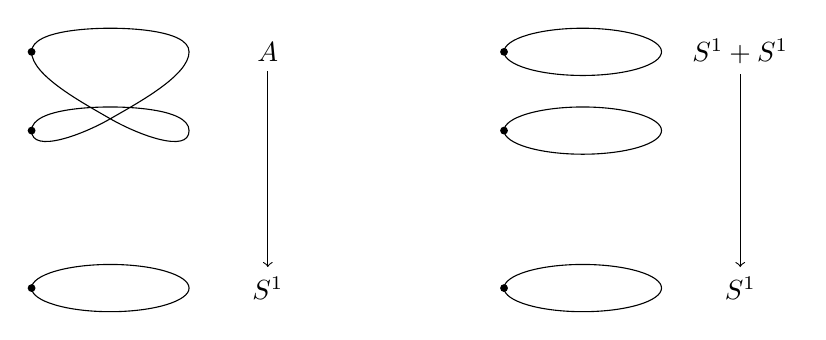
\begin{tikzpicture}
    \node (A) at (2,1) {$A$};
    \node (B) at (2,-2) {$S^1$};
    \draw[->] (A) -- node[auto] {$$} (B);
    \draw (0,-2) ellipse (1 and .3);
    \draw (-1,0)
    .. controls ++( 90:-.3) and ++(210: .4) .. (0,0.15)
    .. controls ++(210:-.4) and ++(270: .3) .. (1,1)
    .. controls ++(270:-.3) and ++(  0: .1) .. (0,1.3)
    .. controls ++(  0:-.1) and ++( 90: .3) .. (-1,1)
    .. controls ++( 90:-.3) and ++(150: .4) .. (0,0.15)
    .. controls ++(150:-.4) and ++(270: .3) .. (1,0)
    .. controls ++(270:-.3) and ++(  0: .1) .. (0,0.3)
    .. controls ++(  0:-.1) and ++( 90: .3) .. (-1,0);
    \node[fill,circle,inner sep=1pt] at (-1,-2) {};
    \node[fill,circle,inner sep=1pt] at (-1,0) {};
    \node[fill,circle,inner sep=1pt] at (-1,1) {};
%    \node (L) at (1,-3) {(left)};
    \begin{scope}[xshift=6cm]
    \node (At) at (2,1) {$S^1+S^1$};
    \node (Bt) at (2,-2) {$S^1$};
    \draw[->] (At) -- node[auto] {$$} (Bt);
    \draw (0,-2) ellipse (1 and .3);
    \draw (0,0) ellipse (1 and .3);
    \draw (0,1) ellipse (1 and .3);
    \node[fill,circle,inner sep=1pt] at (-1,-2) {};
    \node[fill,circle,inner sep=1pt] at (-1,0) {};
    \node[fill,circle,inner sep=1pt] at (-1,1) {};
%    \node (Lt) at (1,-3) {(right)};
    \end{scope}
  \end{tikzpicture}
  \caption{A visualization of two \coverings over the circle}
  \label{fig:covering}
\end{figure}

\begin{remark}
  It \emph{is} possible to misunderstand what a ``connected \covering'' is: 
the other interpretation ``all the preimages are connected'' simply 
would give us an equivalence (since connected sets are contractible),
and this is \emph{not} what is intended. (Equivalences are \coverings, but not necessarily connected \coverings and connected \coverings are not neccesarily equivalences.)  

Likewise, for the other qualifications; for instance in a ``finite covering'' $f:A\to B$, the type $A$ is usually \emph{not} a finite set. 

  We trust the reader to keep our definitions in mind and not the other interpretations.
\end{remark}


\begin{remark}
  \Coverings are closely related to a concept from topology called ``covering space'' (or any variant thereof, including Galois theory) and from algebra as sheaves (of sets).  Either way, the concept is useful because it singles out the (sub)symmetries.  
\end{remark}

% \begin{remark} MB: HAS BEEN MOVED TO A PLACE WHERE IT IS DIRECTLY USED
%\label{rem:setfamloopinj}
% We recall \cref{cor:fib-vs-path} stating that all the fibers of a map $f:A\to B$ 
% are sets if and only if each  $$\ap{f}: (a=a')\to (f(a)=f(a'))$$ is an injection.
%\end{remark}

% \begin{definition}\label{def:decktrafo}\footnote{postpone}
%   Let $f:A\to B$ be a \covering.  A symmetry $(A,f,!)=(A,f,!)$ is called a \emph{deck transformation}.
% \end{definition}
%specified by a pair $(p_A,p_f)$ with consisting of a $p_A:A=_{\UU}A'$, a $p_f:f'p_A=_{A\to B}f$.

\begin{example}\label{xca:coveringsofS1}
Let us consider \coverings over the circle, most conveniently 
for the moment in the guise of families 
$$E:\Sc\to\Set.$$
By circle induction, giving such an $E$ is the same as 
specifying a set $E(\base)$ and a symmetry $E(\Sloop):E(\base)=E(\base)$.  
Said more concisely in terms of \cref{lem:freeloopspace}, 
the type of \coverings over the circle is equivalent to 
$$\sum_{X:\Set}(X=X).$$ \footnote{\color{blue}%
DUPLICATE, BETTER LATER
We will ultimately show that the circle $\Sc$ is equivalent to the 
component (see \cref{def:connected}) $C$ of $(\zet,\etop{s})$ in $\sum_{X:\Set}(X=X)$,  
where $s:\zet\to\zet$ is the successor.  This may seem circular: ``the circle is equivalent to a component of the type of \coverings over the circle!'' 
(MB WHY CIRCULAR: $\sum_{X:\Set}(X=X)$ EXISTS ALSO INDEP OF CIRCLE?)
but it really just condenses the idea that connected groupoids are uniquely 
given by their symmetries.}
\end{example}
A particularly important example is the following:
\begin{definition}\label{def:RtoS1}
Define $R:\Sc\to\UU$ by circle induction by setting 
$R(\base)\defeq\zet$ and $R(\Sloop)\defis \etop{s}$.
Since $\zet$ is a set, and being a set is a proposition,
one can prove by circle induction that $R(z)$ is a set for all $z:\Sc$.
(Abusing notation we also write $R:\Sc\to\Set$.) Now define
$$\RR\defeq\sum_{z:\Sc}R(z)$$
and let the first projection denoted by
$$\exp:\RR\to \Sc$$
be the \emph{exponential \covering of the circle}.
\end{definition}

\begin{remark}
  \label{rem:expforreal}
  The reason for the name $\exp:\RR\to \Sc$ comes from the following visualization.  
%Consider the real and complex numbers $\RR$ and $\mathbb C$.  
If $x$ is a real number, then the complex exponentiation 
$e^{2\pi i x}=\cos(2\pi x)+i\sin(2\pi x)$ has absolute value $1$ and 
so defines a continuous function from the real numbers to the unit circle.  
Choosing any point $z$ on the unit circle, we see that the preimage of $z$ under the exponential function is a shifted copy of the integers inside the reals. 
 
This connection between the integers and the unit circle is precisely captured in a form that we can take further by the \covering $\exp:\RR\to \Sc$.
\end{remark}

We already defined a \covering $f:A\to B$ to be universal if $A$ is connected
and all $a=_A a$ (for $a:A$) are connected. 
If moreover $B$ is a pointed, connected groupoid we shall argue that
we actually can speak of \emph{the} universal \covering.

Recall \cref{cor:fib-vs-path} stating that all the fibers of a map $f:A\to B$ 
are sets if and only if each 
\[
\ap{f}: (a=a')\to (f(a)=f(a'))
\]
is an injection. Assume $B$ is a groupoid.
We prove that $A$ is contractible. 
Being contractible is a proposition, so we may assume 
we have an element $a$ of $A$ since $A$ is connected. 
By \cref{xca:connected-trivia} and \ref{xca:component-connected} 
it suffices to prove that $a=a$ is contractible.
By \cref{xca:prop-set-trivia}, using that $a=a$ is connected,
it suffices to show that $a=a$ is a set.
Using that $\ap{f}$ is an injection, we can apply the remark after
\cref{lem:sum-of-fibers} and obtain that $a=a$ is a set since
$f(a)=f(a)$ is a set, since $B$ is a groupoid.
This completes the proof that $A$ is contractible.

Now assume $(B,b_0)$ is a pointed connected groupoid and $f:A\to B$
a universal \covering. We first prove the proposition $\Trunc{f^{-1}(b_0)}$.
In doing so we may assume an element of $A$. Since $B$ is connected
we have $\Trunc{b_0 = f(a)}$. Again we may assume an element $p: b_0=f(a)$.
Thus $\trunc{(a,p)}:\Trunc{f^{-1}(b_0)}$. 
We can now replay the above argument that $A$ is contractible starting
with a pair $(a,p)$ in $f^{-1}(b_0)$, so that $p: b_0 = f(a)$.
Note that, since $A$ is contractible and $B$ is a groupoid,
$f^{-1}(b)$ is equivalent to the set $b_0 = b$.
This leads to the following definition.\footnote{%
If $B$ is a pointed connected groupoid,
\emph{any} universal \covering is merely equal to \emph{the} universal \covering.
This should be good enough.}

\begin{definition}
  \label{def:universalcover}
  Let $(B,b_0)$ be a pointed connected groupoid.  
The \emph{universal \covering}\footnote{for $B$ not a groupoid this is total misuse of language.  I feel sort of bad about it, but I did not want to say ``path fibration''} of $B$ is the \covering of $B$ given by the family of sets 
  $$\uc{b_0}:B\to\Set,\quad \uc{b_0}(b)\defequi (b_0=_Bb),$$
or alternatively as the first projection from $\uc{b_0}B\defequi\sum_{b:B}(b_0=_Bb)$ to $B$. 
\end{definition}
Note that $(b_0=_B b)$ is a family of \emph{sets} exactly when $B$ is a groupoid. 
However, we have \cref{lem:thepathspaceiscontractible} for any type $B$.

\begin{remark}
  What's so ``universal'' about this?
  %This seems to deflates the concept ``universal \covering'' of a pointed connected groupoid $(B,b_0)$, since we've just shown that t
The universal \covering over the pointed connected groupoid $(B,b_0)$ coincides with the constant function $c_{b_0}:\bn 1\to B$ (with value $b_0$), and seems like an unnecessary complicated representation were it not for the manifold practical value of the formulation that we've given.  
In particular, we recognize the set of symmetries $b_0=_Bb_0$ as the preimage of $b_0$ under the first projection from $\uc{b_0}B$ to $B$; ultimately this will show that the study of symmetries coincides with the study of the universal \covering.

The first instance of this comes already in the next section, where we show in \cref{cor:S1groupoid} that the symmetries of the circle is given by the set of integers $\zet$ by showing that the universal \covering and the exponential \covering (\cref{def:RtoS1}) of the circle coincide.

That said, one way to see that the constant function $c_{b_0}:\bn 1\to B$, \emph{does} deserve the label universal because if given any function $f:A\to B$ and an $(a_0,p): f^{-1}(b_0)$, then we get a function $c_{a_0}:\bn 1\to A$ and $p:b_0=f(a_0)$ gives an element in $c_{b_0}=_{\bn 1\to B}f\, c_{a_0}$.  In other words, any such $f$ is ``a factor of $c_{b_0}$''.  
Note, however, that this depends on $f^{-1}(b_0)$ being non-empty (classically, this is often demanded of a covering, which distinguishes it from our \coverings), and the factorization depends on the element $(a_0,p)$ used. 
\end{remark}



\section{The symmetries of the circle}
\label{sec:pi1S1isZ}\label{sec:symcirc}

With the set $\zet$ of integers \emph{defined} as in \cref{sec:integers}, 
we will now \emph{prove} that $\zet$ is equivalent to the type 
$\base=_{\Sc}\base$, and that under this equivalence $0:\zet$ corresponds to 
$\refl{\base}:\base=\base$, and $1$ to $\Sloop$, and $-1$ to $\Sloop^{-1}$. 
More generally, the successor $\etop{s}:\zet=\zet$ corresponds to composition with $\Sloop$
and the predecessor corresponds to composition with $\Sloop^{-1}$.

The first step is to prove that the exponential \covering \cref{def:RtoS1} 
is equal to the universal \covering in \cref{def:universalcover}, 
\ie we prove that the family 
\[
R: \Sc\to\UU,\qquad R(\base)\defeq\zet,\, R(\Sloop)\defis \etop{s}
\]
is equal to the family
\[
\uc{\base}:\Sc\to\UU,\qquad \uc{\base}(z)\defeq (\base=z).
\]
What does it mean for the families $\uc{\base}$ and $R$ to be equal?
Type families are a special case of functions. 
Function extensionality reduces the question to pointwise equality
of $\uc{\base}$ and $R$ as functions.
Using univalence, it suffices to give
an equivalence from $\uc{\base}(z)$ to $R(z)$, for every $z:\Sc$.

%We define two functions, $f:\uc{\base}\to R$ and $g:R\to \uc{\base}$ and show that, 
% under univalence, they define inverse identities.  

We first recall from \cref{sec:heavy-transport} how 
transport behaves in families of function types.  
Given a type $A$ and two type families $P,Q:A\to\UU$, 
%$P\to Q$ is shorthand for the type $(P\to Q) \jdeq \prod_{a:A}(P(a)\to Q(a)$.  
transport along $p:a=_Aa'$ of $f:P(a)\to Q(a)$ is $Q(p)\,f\,P(p)^{-1}:P(a')=Q(a')$.
In a picture
\[
\xymatrix{
P(a)\ar[rr]^{f}\ar@{=}[d]^{P(p)}_\downarrow&&
  Q(a)\ar@{=}[d]^{Q(p)}_\downarrow\\
P(a')&&\,Q(a').}
\]
If $A$ is $\Sc$, then the induction principle for the circle says 
that giving an $f(z):P(z)\to Q(z)$ for all $z:\Sc$ is the same as 
specifying an $f(\base):P(\base)=Q(\base)$ and an identity 
$f(\Sloop):Q(\Sloop)\,f(\base)\,P(\Sloop)^{-1}=_{P(\base)\to Q(\base)}f(\base)$,
\ie a witness that the composites in 
$$\xymatrix{
  P(\base)\ar[rr]^{f(\base)}\ar@{=}[d]^{P(\Sloop)}_\downarrow
 &&Q(\base)\ar@{=}[d]^{Q(\Sloop)}_\downarrow\\
  P(\base)\ar[rr]^{f(\base)}&&\,Q(\base)}
$$
are equal.  If $P,Q$ are families of sets, 
then the type of $f(\Sloop)$ is a proposition.

We now define two fiberwise maps that will turn out to give
inverse equivalences between $\uc{\base}(z)$ and $R(z)$, for each $z:\Sc$.

\begin{definition}
  \label{def:fPtoR}
  The function $f:\prod_{z:\Sc}(\uc{\base}(z)\to R(z))$ is defined by transport: $f(z)(p)\defequi\trp{R,p}(0)$.
\end{definition}

In Figure~\ref{fig:transportalongloop}, the transport in the definition
above has been visualised for $p={\Sloop^n}$, $n=-2,-1,0,1,2$.

\begin{figure}[h]
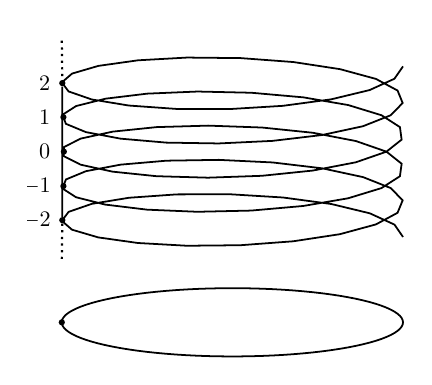
\begin{tikzpicture}[scale=0.8]
\begin{axis}[axis lines=none,line width=1pt, axis equal image]

\node at (-10,13) () {$\zet$}; %CUTOFF FOR UNKNOWN REASON
\node [] at (-10,12) (A) {};

\addplot[domain=0:10*pi,samples=100,black,no marks,thick] %500 samples slow
({10*cos(deg(x))}, % x-coordinate
{2*sin(deg(x)) + x/pi}) % y-coordinate
node [circle,scale=0.3,fill,pos=0.9] (B) {} % point (A)
node [circle,scale=0.3,fill,pos=0.7] {} % point (A)
node [circle,scale=0.3,fill,pos=0.5] {} %
node [circle,scale=0.3,fill,pos=0.3] {} % 
node [circle,scale=0.3,fill,pos=0.1] (C) {}; %

\node at (-11,9) () {$2$};
\node at (-11,7) () {$1$};
\node at (-11,5) () {$0$};
\node at (-11,3) () {$-1\;\;\,$};
\node at (-11,1) () {$-2\;\;\,$};

\node [] at (-10,-2) (D) {};
\node at (0,-5) () {$\Sc$};
\node at (9,-5) () {$\Sloop$};

\addplot[domain=0:2*pi,samples=100,black,no marks,thick] %500 samples slow
({10*cos(deg(x))}, % x-coordinate
{2*sin(deg(x))-5}) % y-coordinate
node [circle,scale=0.3,fill,pos=0.5] (E) {}; % point (D)


\draw[dotted] (A)--(B);
\draw[thick] (B)--(C);
\draw[dotted] (C)--(D);

\end{axis}
\end{tikzpicture}
\caption{Transport in the family $R$}
\label{fig:transportalongloop}
\end{figure}

\begin{lemma}\label{lem:windingnumber}
For $f$ as in \cref{def:fPtoR} we have $f(\base)(\Sloop^n)=n$ for all $n:\zet$.
\end{lemma}
\begin{proof}
By induction on $n:\zet$.  In the base case $n=0$ we have
$f(\base)(\Sloop^0)\defeq f(\refl\base)\defeq 0$.
For $n=s(m)$ with $m:\NN$ we have\footnote{some references needed here} 
\begin{align*}
  f(\base)(\Sloop^{s(m)})&\defeq\trp{R,\Sloop^{s(m)}}(0)\\
  &=\trp{R,\Sloop \Sloop^{m}}(0)\\
  &=\trp{R,\Sloop}(\trp{R,\Sloop^m}(0))\\
  &=s(\trp{R,\Sloop^m}(0)).
\end{align*}
The last equality follows from $\etop{s}=R(\Sloop)$ using
$s=\cast(\ua(s))=\cast(\etop{s})=\trp{\id_\UU,\etop{s}}=\trp{R,\Sloop}$, 
see \cref{def:idtoeq} and \cref{def:univalence}.
For negative $n$ the proof is similar.
\end{proof}

In the definition of the second map, 
take into account that $R(\base)\jdeq \zet$ and $\uc{\base}(\base) \jdeq (\base=\base)$.

\begin{definition}\label{def:gRtoP}
The function $g:\prod_{z:\Sc}(R(z)\to \uc{\base}(z))$ is 
defined by circle induction: 
\[
g(\base)\defeq {\Sloop^{-}}:\zet\to(\base=\base) : n \mapsto {\Sloop^n}
\]
and 
\[
g(\Sloop): \uc{\base}(\Sloop)\, g(\base)\,R(\Sloop)^{-1}=_{\zet\to (\base=\base)} g(\base).
\]
So far we have only given the type of $g(\Sloop)$. By definition, $R(\Sloop)$ is $s$
and $\uc{\base}(\Sloop)$ is composition with $\Sloop$.
In a picture, $g(\Sloop)$ should prove that it does not matter what 
path you take around the square
$$\xymatrix{\zet\ar[rr]^{\Sloop^-}\ar@{=}[d]^s_\downarrow
 &&(\base=\base)\ar@{=}[d]^{\Sloop\cdot\_}_\downarrow\\
  \zet\ar[rr]^{\Sloop^-}&&\,(\base=\base).}
$$
This follows by a simple calculation: ${\Sloop\,\Sloop^{n-1}} = {\Sloop^n}$, 
for all $n:\zet$. 
\end{definition}


\begin{lemma}
  \label{lem:univisexp}
For every $z:\Sc$, the functions $f(z)$ defined in \cref{def:fPtoR} 
and $g(z)$ in \cref{def:gRtoP} are inverse equivalences between
$\uc{\base}(z)$ and $R(z)$.
%$\uc{\base}$ defines a connected \covering of the circle: $\uc{\base}(z)\defeq (\base=z)$ is a set for all $z:\Sc$ and the type $\uc{\base} \Sc$ is connected (more precisely, by univalence $\uc{\base}(z)$ is equal to the set $R(z)$ and $\uc{\base} \Sc$ is contractible).
\end{lemma}
\begin{proof}
We apply \cref{lem:weq-iso} and verify the two conditions.
  Firstly, we need to give elements $H(z,p):g(z)(f(z)(p))=p$
for all $z:\Sc$ and $p:\uc{\base}(z)\defeq(\base=z)$. 
By induction on $z$ and $p:\base=z$ it suffices to set 
$H(\base,\refl\base)\defeq\refl{\refl{\base}}$ since
$g(\base)(f(\base)(\refl{\base}))\jdeq g(\base)(0)\jdeq\refl{\base}$.

Secondly, we need to give elements $G(z)(n):f(z)\,g(z)(n))=n$
for all $z:\Sc$ and $n: R(z)$.
By circle induction it suffices to define $G(\base)$ and $G(\Sloop)$,
but since $\zet$ is a set the information for $G(\Sloop)$ is redundant.
Hence, we need to show that for all $n:\zet$ that 
$f(\base)(g(\base)(n))\jdeq  f(\base)(\Sloop^n)$ is equal to $n$.  
This follows from \cref{lem:windingnumber}. 
\end{proof}


\begin{corollary}\label{cor:S1groupoid}
The circle $\Sc$ is a groupoid, and the function
%$\uc{\base}$ is a \covering, NOT NEEDED
\[
{\Sloop}^{-} : \zet\to(\base=_{\Sc}\base) %\text{sending $n$ to ${\Sloop}^n$}
\]
sending $n$ to $\Sloop^n$ is an equivalence.
\end{corollary}
\begin{proof}
For any $z:\Sc$, the type $\uc{\base}(z)\jdeq (base=_{\Sc}z)$ is a set 
since $R(z)$ is a set and $\uc{\base}(z) \equiv R(z)$.
Since the circle is connected and being a set is a proposition, it follows
that $y=_{\Sc}z$ is a set, for any $y,z:\Sc$. Hence $\Sc$ is a groupoid.
By \cref{def:gRtoP}, ${\Sloop}^{-}\jdeq g(\base)$ is an equivalence.
\end{proof}


\section{A reinterpretation of the circle}
% and a criterion for equivalence through \coverings}
\label{sec:S1isC}
In this section we return to the considerations discussed in \cref{xca:coveringsofS1}.
Through \cref{lem:freeloopspace} we can get a different perspective on the circle which highlights it as a type classifying very simple symmetries.
By \cref{lem:freeloopspace} (moving up one universe), a type family $\Sc\to\UU$ is uniquely given by a type $X:\UU$ together with a $i:X=_\UU X$, with no further requirements on $i$.
Using UA, any type $X$ and any equivalence $f: X\equiv X$ provides such a pair
$(X,\etop{f})$. We have seen one example in \cref{def:RtoS1}, 
namely the set $\zet$ of integers together with the successor $s: \zet\equiv\zet$.

The importance of the latter example will become apparent when we eventually 
explain that \emph{the circle is equivalent to the connected component of 
$(\zet,\etop{s})$ in the type $\sum_{X:\UU}(X=_{\UU}X)$}. 

Heading towards this goal, we investigate this component a bit further.
Define the type family $D$ by $D(X) \defeq (X=X)$ for all $X:\UU$.
Recall from \cref{lem:isEq-pair=} that, given $X:\UU$ and $i: X=X$, 
the identity type $(\zet,\etop{s}) = (X,i)$
is equivalent to the type of pairs consisting of a $p:\zet=X$ and 
a proof of $\pathover{\etop{s}}{D}{p}{i}$. The latter type is
equivalent to $\trp{D,p}(\etop{s}) = i$ by \cref{def:pathover-trp}.
The transport is by conjugation,
\cref{xca:trp-in-a/x=b/x}(\ref{trp-in-x=x}), so that the latter
type is equivalent to $p\cdot\etop{s}\cdot p^{-1} = i$, 
and to $p\cdot\etop{s} = i\cdot p$, or $p \etop{s} = i p$ for short. 
In total, the identity type $(\zet,\etop{s})=(X,i)$ is equivalent to
\[
\sum_{p: {\zet = X}} {p \etop{s}} =_{\zet=X} {i p}.
\] 
Since $\zet$ is a set, this sum type is a set.
In particular, the type of symmetries $(\zet,\etop{s})=(\zet,\etop{s})$
is equivalent to the set $\sum_{p:\zet=\zet}p\etop{s}=\etop{s}p$.  

% and so our component $C$ is a connected groupoid. LATER FROM C=S1

This discussion tells us that the following definition makes sense:

\begin{definition}\label{def:S1toC}
Let $C$ be the component of $\sum_{X:\UU}(X=_{\UU}X)$ containing $(\zet,\etop{s})$.
Define by circle induction
\[
c:\Sc\to C \text{~setting~} 
c(\base)\defequi (\zet,\etop{s},\trunc{\refl{(\zet,\etop{s})}})
\]
and $c(\Sloop): c(\base)=_C c(\base)$ given by the successor 
$\etop{s}:\zet=\zet$ and trivial proofs of the proposition
$\etop{s}\etop{s}=\etop{s}\etop{s}$ and the proposition for the 
truncated third component of $c(\base)$.
\end{definition}

We will henceforth leave out the third component from the denotation
of elements of $C$, since its type is propositional and does not convey 
any information beyond its mere existence. We may write a ``!'' in order
to remind the reader of hidden information of propositional type.
  
We start by identifying the symmetries of $(\zet,\etop{s})$ in $C$:

\begin{lemma}
  \label{lem:IdCisZet}
Any element in $(\zet,\etop{s})=_C(\zet,\etop{s})$ is of 
the form $\pathpair{\etop{s}^k}{!}$ for some unique $k:\zet$.  
In other words, the function 
\[
\ev_0:((\zet,\etop{s})=_C(\zet,\etop{s}))\to \zet 
\text{~defined by~} \ev_0(\pathpair{p}{!}) \defeq \ptoe{p}(0)
\]
is an equivalence.
\end{lemma}
\begin{proof}
  Given $\pathpair{p}{!}:(\zet,\etop{s})=_C(\zet,\etop{s})$ we must determine 
$p:\zet=\zet$. By univalence this amounts to giving all the values 
$\ptoe{p}(n)$ for $n:\zet$.  However, since $s\ptoe{p}=\ptoe{p}s$ we 
get that $\ptoe{p}(n+1)=\ptoe{p}(n)+1$ for all $n:\zet$. 
Induction on $n:\zet$ (positive and negative $n$ separately) gives that 
$\ptoe{p}(n)=n+\ptoe{p}(0)$. Hence $\ptoe{p}=s^{\ptoe(0)}$, so $p=\etop{s}^k$
for some unique $k:\zet$.
\end{proof}

We are going to prove that $c$ is an equivalence.
The method of proof will be used on several occasions.
Therefore we isolate the following general result first.

\begin{lemma}\label{lem:conn-eq-f-ap-f-x}
Let $X$ and $Y$ be connected types, $x$ an element of $X$,
and $f$ a function from $X$ to $Y$. Then $f$ is an equivalence
if and only if $\ap{f}: (x=x) \to (f(x)=f(x))$ is an equivalence.
\end{lemma} 
\begin{proof}
Using \cref{cor:fib-vs-path}(\ref{conn-fib-vs-path}) it suffices to show that 
each $\ap{f}$ is an equivalence if and only if the specific $\ap{f}$ with 
domain $x=x$ is an equivalence. Being an equivalence is a proposition, 
so this follows in two easy steps from $X$ being connected,
using \cref{xca:component-connected}.
\end{proof}

\begin{theorem}\label{thm:S1bysymmetries}
  The function $c:\Sc\to C$ from \cref{def:S1toC} is an equivalence.
\end{theorem}
\begin{proof}
  In view of \cref{lem:conn-eq-f-ap-f-x} we only need to show that 
$\ap{c}:(\base=_{\Sc}\base)\to((\zet,s)=_C(\zet,s))$ is an equivalence.
\footnote{ ((can we call equivalences between sets bijections?)). YES, BUT NOT NEEDED}
Note that both the domain and the co-domain of $\ap{c}$ is equivalent to $\zet$.
Consider the following diagram in which we compose $c$ with the equivalences
from \cref{cor:S1groupoid} and \cref{lem:IdCisZet}:
\[
\xymatrix{
\zet\ar[rr]^-{\Sloop^{{-}}}&&
(\base=\base)\ar[rr]^-{\ap{c}}&&
((\zet,s)=_C(\zet,s))\ar[rr]^-{\ev_0}&&
\zet}
\]
For $c$ to be an equivalence, it suffices to show that the composition
is the identity on $\zet$. By definition $\ap{c}(\Sloop) = \pathpair{\etop{s}}{!}$, 
and by induction on $n:\zet$
one shows  $\ev_0(\ap{c}(\Sloop^n))=\ev_0(\pathpair{\etop{s}^n}{!}) = s^n(0) = n$. 
% The composition with the functions $\Sloop^-:\zet\to (\base=_{\Sc}\base)$ sending $n:\zet$ to $\Sloop^n$ and $\ev_0:((\zet,s)=_C(zet,s))\to \zet$ of \cref{lem:IdCisZet} given by $\ev_0(p)=p(0)$ gives us a function $w:\zet\to\zet$ with $w(n)=s^n(0)$.  From \cref{cor:S1groupoid} we know that $\Sloop^-$ is an equivalence, so we only need to show that $w$ is an equivalence
\footnote{I may have used 2-out-of-3 before, we probably need to include it somewhere, though by univalence it hardly seems necessary}% .  If $p:\zet=\zet$ with $!:sp=ps$, we get by induction on $n:\zet$ (induction for positive and negative $n$ separately) that $p(n)=n+p(0)$.  Hence, all the elements in the preimage $w^{-1}(p,!:sp=ps)$ are equal to $(p(0),!)$.  
\end{proof}

% Now, consider the function 
% $$f:\sum_{p:\zet=\zet}(sp=ps)\to\zet,\qquad f(p,!)=p(0).$$  If $a:\zet$, then $f^{-1}(a)$ consists of the $p:\zet=\zet$ with $sp=ps$ and $p(0)=a$ (the last two are propositions), but by induction we see that $p(n)=n+a$ for all $n:\zet$ (separate induction on positive and negative numbers).  In other words, all elements in the set $f^{-1}(a)$ are equal, and so $f$ is an equivalence


%   ((TODO))
% As an illustration of things to come in a simpler setting, we can give the torsor definition of the circle, where Marc makes the simplifying observation that (since the integers is free on one generator) this can be coded in terms of the successor and there is a priori no need to talk about the abstract group.  In short: an (abstract) $\ZZ$-set is uniquely given by a set $X$ with an identity $f: X=_{\Set}X$.  A $\ZZ$-torsor $(X,f)$ is a $\ZZ$-set (merely) equal to $(\zet,S)$ ($S$ is the successor), that, there is a $p:X=\zet$, so that $Sp=_{X=X} pf$.  This is based at (the pricipal $\ZZ$-torsor represented by) $(\zet,S)$ and $(\zet,S)=(\zet,S)$ consists of $f:\zet=\zet$ s.t. $Sf=fS$.  Such an $f$ must be given by addition by the integer $f(0)$.  This gives us an equivalence between $\Sc$ and the type of (secret) $\ZZ$-torsors.  This will be trivial if we have shown that a map of connected groupoids is an equivalence if it induces an equivalence on the identity sets.

\section{Other \coverings over the circle}
\label{sec:covS1}

Let $A$ be a type and $f:A\to \Sc$ a function.
By \cref{cor:fib-vs-path}(\ref{set-fib-vs-path}), $f$ is a \covering
over $\Sc$ if and only if each $\ap{f}$ is injective.
Assume that $f:A\to \Sc$ is a \covering with $A$ is connected.
Let $(a_0,p)$ be an element of $f^{-1}(\base)$. 
By \cref{xca:component-connected}
the condition that \emph{each} $\ap{f}$ is injective
can be relaxed to $\ap{f}: (a_0=a_0)\to(f(a_0)=f(a_0))$ being injective.
Now look at the following subset:
\[
\set{~ l: \base = \base \mid {\ap{f}}^{-1}(plp^{-1})~ }.
\]
Clearly, a classification of connected \coverings over the circle
also classifies certain subsets of symmetries of $\base$.
Such subsets are closed under concatenation and inverses,
since $\ap{f}$ is compatible with these operations,
see \cref{lem:apcomp}.\footnote{%
Using language yet to be introduced, we actually classify the subgroups of the integers.}
We start by giving some examples of connected \coverings of the circle.
In the course of our discussion, we will see that -- assuming a weak form
of the Law of the Excluded Middle -- these are all the decidable connected 
\coverings over the circle.

\begin{example}\label{exa:univS1cover}
The \emph{universal} \covering from \cref{def:universalcover}
is the map $c_\base:\bn 1\to \Sc$ 
sending the unique element of $\bn 1$ to $\base$. 
(It takes this simple form since the circle is a pointed connected
groupoid, see the discussion before \cref{def:universalcover}.)
The universal \covering corresponds to the subset consisting 
of $\refl\base : \base=\base$ only.  
\end{example}

\begin{example}\label{exa:mfoldS1cover}
For $m:\NN$ positive, define the \emph{degree $m$ function} by circle induction
\[
-^m:\Sc\to \Sc, \text{~~setting~} 
-^m(\base)\defeq\base \text{~~and~} 
-^m(\Sloop)\defis{\Sloop}^m.
\]
This \covering corresponds to the subset consisting 
of ${\Sloop}^{mn} : \base=\base$ for all $n:\zet$.
\end{example}

Note that the degree $0$ function would be constant,
and hence not a \covering since the domain is not a set,
see \cref{xca:constant-cover}

\begin{remark}
  \label{rem:RtoS1}
The universal \covering is essentially the same as defined in \cref{def:RtoS1}
and explained in \cref{rem:expforreal}
since the real numbers form a contractible space.

\label{rem:finitecoveringsofS1}
The analogue of our degree $m$ function is the $m$-th power of complex numbers 
restricted to the unit circle. % mapping $z$ to $z^m$ if $|z|=1$.  
The following visualization is perhaps more tangible.  
Let $m=12$ and picture the circle and mark $12$ evenly spaced points.
This will look like a clock, with marks $1,2,\dots,12$. 
You can then make a function from the circle to itself by sending 
all marks to $12$ and each of the arcs connecting the marks to the entire circle 
-- (in a continuous manner preserving the orientation).
  ((picture!!))
\end{remark}

We could be more ambitious and ask: what is the \emph{type} of decidable 
\coverings over the circle?  Since the type of \coverings is 
equivalent to $\Sc\to \Set$, and $\Set$ is a groupoid
(\cref{lem:Set-is-groupoid}),
\cref{lem:level-n-utils}(\ref{level-n-utils-codom}) gives
that the type of decidable \coverings over the circle is a groupoid.  
We will pin this groupoid down by first identifying the components 
(of which there turns out to be one for each natural number), 
and then analyzing one component at a time.

Recall the function $c:\Sc\to C$ of \cref{def:S1toC}. 
By \cref{thm:S1bysymmetries} we know that $c$ is an equivalence, 
so classifying \coverings over $\Sc$ is equivalent to 
classifying \coverings over $C$.  
We simplify the notation slightly, letting $\pt_C\defeq(\zet,\etop{s}):C$ 
(so that $\pt_C \jdeq c(\base)$ with $c$ from \cref{def:S1toC}), 
and allowing ourselves to write $s:\pt_C=_C\pt_C$ instead of the 
more honest $\pathpair{\etop{s}}{!}:\pt_C=_C\pt_C$ 
(equal to the $c$-image of ${\Sloop}:\base=\base$).

It is instructive to rephrase the examples of connected \coverings over $\Sc$ in 
terms of $C$, even though they could be transported along $\Sc=C$.

\begin{example}\label{exa:univCcover}
The universal \covering is represented by the constant function
$c_{(\zet,\etop{s})}:\bn 1\to C$ sending the unique element 
of $\bn 1$ to $(\zet,\etop{s}):C$.
\end{example}

\begin{example}\label{exa:mfoldCcover}
Assume that $m:\NN$ is positive.  We give a description of 
the $m$-fold \covering over the circle in terms of $C$.
{\color{red} There are several interesting aspects. First,
for $\Sc$ we have $\base\jdeq-^m(\base)$ and for $C$, as we
will see, we get $(\zet,\etop{s}) = -^m(\zet,\etop{s})$, 
with $=$ and not with $\jdeq$.
Let's say $-^m(\zet,\etop{s})\jdeq(Y,\etop{r})$.
The loop of $(\zet,\etop{s})$ is based on $s$,
the corresponding loop of $(Y,\etop{r})$ is based on $r$.
The challenge is to arrange things in such a way that
$-^m$ acting on $s$ yields $r^m$.
This motivates the following definition.}

For any type $X$ and $f:X\to X$, we define the $m$-th \emph{root}
\[
{\sqrt[m]f} : {\bn m\times X} \to {\bn m\times X}
\]
of $f$ by setting 
\[
\sqrt[m]f(i,x)\defeq
\begin{cases}
  (i+1,x)& \text{for $i<m-1$ and}\\
  (0,f(x))& \text{for $i=m-1$}.
\end{cases}
\] 
Only one $m$-th of the time does $\sqrt[m]f$ use $f:X\to X$,
the rest of the time it increases the element in $\bn m$).
This is illustrated in \cref{fig:root} with the shift by $f$ being 
vertical and the movement along $\bn m$ going around a circle.  
\begin{figure}[bt]
  \centering
  \begin{tikzpicture}
    \node (A) at (4,1) {\quad$\sqrt[m]f:{\bn m\times X}\to{\bn m\times X}$};
    \foreach \y in {0,1,2}
    { \begin{scope}[shift={(0,\y)}]
        \foreach \x in {0,...,4}
        { \node[fill,circle,inner sep=1pt] at (180+72*\x:1 and .3) {}; }
        \foreach \x in {0,...,3}
        { \draw[-stealth] (180+72*\x:1 and .3) arc(180+72*\x:252+72*\x:1 and .3); }
      \end{scope} }
    \foreach \y in {1,2}
    { \begin{scope}[shift={(0,\y)}]
        \draw[-stealth] (108:1 and .3)
        .. controls ++( 5:-.3) and ++(80:.2) .. (-.7,-.4)
        .. controls ++(80:-.2) and ++(90:.2) .. (-1,-1);
      \end{scope} }
    \draw[-stealth] (108:1 and .3)
    .. controls ++( 5:-.3) and ++(80:.2) .. (-.7,-.4);
    \node (dz) at (-.7,-.7) {\footnotesize$\vdots$};
    \begin{scope}[shift={(0,3)}]
      \draw[-stealth] (-.7,-.4)
      .. controls ++(80:-.2) and ++(90:.2) .. (-1,-1);
      \node (da) at (-.7,0) {\footnotesize$\vdots$};
    \end{scope}
    \draw [decorate,decoration={brace,amplitude=10pt}]
    (-1.1,-.8) -- (-1.1,2.8) node [black,midway,xshift=-20pt] {\footnotesize $X$};
    \draw [decorate,decoration={brace,amplitude=10pt}]
    (1,-1) -- (-1,-1) node [black,midway,yshift=-15pt] {\footnotesize $\bn{m}$};
  \end{tikzpicture}
  \caption{The $m$-th root of a function $f: X\to X$}
  \label{fig:root}
\end{figure}
Indeed, iterating $\sqrt[m]f$ we get $(\sqrt[m]f)^m(i,x)=(i,f(x))$; 
hence the term ``$m$-th root'' is apt.

If $f$ is an equivalence, then so is $\sqrt[m]f$:
\begin{enumerate}
\item on one hand $(\sqrt[m]f)(j,y)$ is equal to $(0,x)$ if and only 
if $j=m-1$ and $f(y)=x$, so  $(\sqrt[m]f)^{-1}(0,x)$ is equivalent 
to $f^{-1}(x)$ which is contractible if $f$ is an equivalence, and 
\item on the other, if $i:\bn m$ is not $0$, then $(\sqrt[m]f)(j,y)$ is equal 
to $(i,x)$ if and only $j+1=i$ and and $y=x$, 
and so  $(\sqrt[m]f)^{-1}(i,x)$ is equivalent to  a singleton.
OK FOR ANY *TYPE* X
\end{enumerate}

Using univalence, the $m$-th root construction applies not only to equivalences, 
but equally well to identities $f:X=X$, resulting in a function 
\[
-^m:\sum_{X:\UU}(X=X)\to\sum_{X:\UU}(X=X),\quad -^m(X,f)\defeq(\bn m\times X,\sqrt[m]f).
\]
We now focus on  $C$, the component of $\sum_{X:\UU}(X=X)$ containing $(\zet,\etop{s})$.
Note that the function $\mZ : (\bn m\times \zet) \to \zet$ 
given by $\mZ(i,n)=i+mn$ is an equivalence. 
Moreover we have ${\mZ\!\!\sqrt[m]s} = {s\mZ}$ since 
\[
\mZ(\sqrt[m]s(i,n)) = i+1+mn = s(\mZ(i,n))
~~\text{for all $(i,n):\bn m\times \zet$}.
\]  
Hence $ -^m(\zet,\etop{s}) \jdeq (\bn m\times\zet,\sqrt[m]{\etop{s}}) = (\zet,\etop{s})$. 
If $(\zet,\etop{s})=(X,f)$, then $-^m(\zet,\etop{s})=-^m(X,f)$, 
so $(\zet,\etop{s})=-^m(X,f)$. Hence we can actually restrict the
\emph{degree $m$ function} to the component $C$\footnote{\color{red}%
Note to BID: what about this phrasing, not mentioning truncation?}
: 
\[
-^m:C\to C,\qquad -^m(X,f)\defeq(\bn m\times X,\sqrt[m]f).%,~~\text{for all $(X,f):C$}.
\]
All reincarnations of the degree $m$ function are denoted the same.

% In consequence, if $(X,f):C$ (\ie $(X,f):\sum_{X:\Set}X=_\UU X$ is in the component of $(\zet,s)$) then also $(\sqrt[m]X,\sqrt[m]f):C$, giving rise to the 
%
% , where $$\sqrt[m]X=\bn m\times X$$ and $\sqrt[m]f(i,x)=(i+1,x)$ for $i<m-1$ and $\sqrt[m]f(m-1,x)=(1,f(x))$.  We prove that $-^m((X,f))$ is in the component of $(\zet,s)$ (which was a requirement for elements in $C$).
 % Since we know that $(X,f)$ is in the component of $(\zet,s)$ it is enough consider the element $(p,!):(\sqrt[m]{\zet},\sqrt[m]s)=(zet,s)$ explicitly given by univalence through $p((i,n))=i+mn$ ((check that it gives an equivalence)).

We now analyze how $-^m$ acts on paths. Let $(\etop{p},!):(X,f)=_C(X',f')$.
Since $-^m$ maps first components $X$ to $\bn m\times X$, we get that
the first projection of $\ap{-^m}(\etop{p},!)$ is 
$\overline{\id\times p} : (\bn m\times X) = (\bn m\times X')$.
We are particularly interested in the case of the loop of $C$, 
that is, $(\etop{s},!):(\zet,\etop{s})=_C(\zet,\etop{s})$.
We calculate $(\id\times s)(i,n) = (i,s(n))$,
which by the property of the $m$-root is equal to $(\sqrt[m]s)^m(i,n)$.
So we have $(\id\times s)=(\sqrt[m]s)^m$, which means that
$\ap{-^m}(\etop{s},!)$ is indeed the $m$-power of the
loop of $(\bn m\times \zet,\sqrt[m]{\etop{s}})$.

%$$(\id\times p,!):(\bn m\times X,\sqrt[m]f)=(\bn m\times X',\sqrt[m]f')$$
\footnote{\color{red}%
Fact $!:(\id\times p)\sqrt[m]f=_{\bn m\times X=\bn m\times X'}\sqrt[m]{f'}(\id\times p)$
since $(i,x)$ is taken to $(i+1,px)$ if $i<m-1$, and $(m-1,x)$ is taken to $(0,f'px)$
and $(0,pfx)$, respectively, which are equal by assumption NOT USED, THIS HOLDS
BY THE ACTION ON PATHS} 


This will eventually ((forwardref)) be explained in terms of the symmetries of the 
degree $m$ \covering of the circle being given by the powers of $\sqrt[m]s$ in a 
nonunique fashion: for any $a:\zet$, the $a$-th and the $(a+m)$-th power of 
$\sqrt[m]s$ give rise to the same symmetry.

Why does this correspond to the $m$-fold \covering we defined in \cref{exa:mfoldS1cover}?  
This is encapsuled by the fact that under the equivalence $c:\Sc\to C$ the two $m$-fold covers agree in the sense that the two functions given as composites in
$$\xymatrix{\Sc\ar[r]^c\ar[d]^{-^m}&C\ar[d]^{-^m}\\\Sc\ar[r]^c&C}$$ are equal.  One composite is given by $-^mc(\base)=(\zet,s)$ and $-^mc(\Sloop)=s^m$ and the other is given by $c-^m(\base)=(\bn m\times\zet,\sqrt[m]s)$ and $c-^m(\Sloop)=\id\times s$ 
({\color{red} interchanged?})
and the proof that these two functions are equal is given by the (identity corresponding by univalence to the) equivalence  $\mZ: (\bn m\times \zet)\to\zet$ with $\mZ(i,n)=i+mn$ discussed above, since transport of $\sqrt[m]s$ along $\mZ$ is exactly $s^m$ (\ie, $\mZ\cdot\sqrt[m]s=s^m\cdot\mZ$,
({\color{red} I think $s^m$ should twice be $s$, and that the cicle induction requires that $\mZ$ is invariant under $\Sloop$, see kladdeark when we talk})
note the way we formulate this so that we don't need to talk about an inverse of $\mZ$).
\end{example}

\begin{xca}
Check the implicit claims in \cref{exa:mfoldCcover}.  ((perhaps best to make them explicit?))
\end{xca}

There are many instances of the $m$-th root construction which is of independent interest.  
We record the following for future reference.
\begin{definition} \label{def:Zetmodm}
Let $m$ be a positive integer.
The element $\zet/m:\sum_{X:\Set}(X=X)$ has first projection $\bn m\times\bn 1$ and 
second projection $\sqrt[m]{\id}$.
\end{definition}
This realizes the cycle $0\mapsto1\mapsto\dots\mapsto m-1\mapsto 0$ in $\bn m$, and so models ``modular arithmetic''.


Any (other) textbook will tell you that these are all the connected \coverings over the circle (precisely one for each natural number), but the procedure is unfortunately not constructive: we need a further assumption which is not generally present in our setup, namely

\begin{quote}
  {\bf The Limited Principle of Omniscience} (LPO)\index{LPO}\label{LPO}\footnote{make an environment that principles can fit in and be numbered} If given a function $P:\NN\to\bn 2$, then either $P$ is constant (we have that $\prod_{n:\NN}(P(0)=P(n))$) or there is an $n_0:\NN$ such that $P(n_0)\neq P(0)$.
\end{quote}
LPO is weaker than the law of excluded middle and we are free to assume it as an axiom -- or not.  We will be explicit about where we will use it.


Fix for the moment a connected type $A$ and a decidable \covering 
$$f:A\to C$$ (c.f \cref{def:covering}) and an element $\pt_A:f^{-1}(\pt_C)$.  %Assume $(\pt_A,!):f^{-1}(\pt_C)$
%Recall the element 
%$$\pt_C\defequi(s,\refl{ss}):(\zet,s)=_C(\zet,s),$$ which by \cref{def:S1toC} corresponds to $\Sloop:\base=\base$.
By \cref{lem:eqandcovofconntypes}, the fact that $f$ is a decidable \covering exactly says that the induced function of identity types
$$g\defequi\ev_0f^=:(\pt_A=_A\pt_A)\to (\pt_C=_C\pt_C)=\zet$$ is 
injective and (the fibers are) decidable.\footnote{say this in a way consistent with the choices of subsets/injections/embeddings}    

Assume LPO.  We are then left with two situations (use that $g$ is injective and decidable): either $\pt_A=_A\pt_A$ is contractible or there is a $p_0:\pt_A=_A\pt_A$ with $g(p_0)$ different from $0$. 

In the former case ($\pt_A=\pt_A$ is contractible), \cref{lem:eqandcovofconntypes} together with the fact that $A$ is connected implies that $A$ itself is contractible.  

On the other hand, if $p_0:\pt_A=\pt_A$ with $g(p_0)$ different from $0$, then either $g(p_0)$ or $g(p_0^{-1})$ is a positive integer.  Hence the set $H^+$ of positive integers in the image of $g$ is nonempty, and so the fact \cref{def:Nwellordered} that $\NN$ is well ordered implies that $H^+$ has a minimum, \ie there is a $p:\pt_A=\pt_A$ with  $g(p)=m\defequi\min H^+:H^+$.  Furthermore, if $q:\pt_A=\pt_A$ is any element with $0<g(q)$, then  by Euclidean division of \cref{lem:euclid-div}, there exist $k,r:\NN$ with $r<m$ so that $g(q)=km+r$.  Now, the natural number $r$ is in the image of $g$ (because $r=g(q)-km=g(qp^{-k})$) and is less than the minimal positive value $m=g(p)$, and so we must conclude that $r=0$, or in other words, $g(q)$ is a multiple $g(p)k$ of the minimal positive value $g(p)$.

% \cref{cor:arch} there is a $k:\NN$ such that $g(p)k\leq g(q)<g(p)(k+1)$, or equivalently $0\leq g(q)-g(p)k< g(p)$.  Since $g(q)-g(p)k=g(qp^{-k})$ is a nonnegative integer is in the image of $g$ and simultaneously less than the minimum positive value $g(p)$, we must conclude that $g(q)=g(p)k$.\footnote{rewrite/simplify given that Euclid is now in intro}

Arguing similarly for the negative values, we reach the conclusion that the image of $g$ in $\zet$ is the subset of multiples of $g(p)=\min H^+$.  Hence, the image of $f^=:(\pt_A=\pt_A)\to(\base=_{\Sc}\base)$ is uniquely given by the positive integer $\min H^+$, and is not dependent on $\pt_A$.\footnote{how to say this gently without starting to much fuss regarding commutativity?}  Furthermore, if $p_A:A=_{\UU}A'$, $f':A'\to B$ and $p_f:f'p_A=_{A\to B}f$, then tracing through the argument, we see that the positive number reached through arguing with $f':A'\to B$ remains the same, but there \emph{is} a possibility that $g(p_0)$ changes sign, so that the minimum of $H^+$ is now not attained by $g(p_0)$, but by $g(p_0^{-1})$.\footnote{maybe some HoTT guy can say this less classically.  We also want to say something about the connection to pointed \coverings, conjugations etc to clear the path for later applications}

\begin{lemma}
  \label{lem:componentsofcoversofS1}
  % Assume the LPO. Given a connected decidable \covering of the circle,  there is a unique natural number $m$ so that the connected \covering is equal to the connected \covering $-^m$ of \cref{exa:listofS1covers}.  This gives an equivalence between $\NN$ and the propositional truncation of the type of connected decidable \covering of the circle.
  \begin{enumerate}
  \item The type of decidable \coverings over the circle by connected types is a groupoid.
  \item Assuming, the LPO the type of decidable \coverings over the circle by connected types is the sum of the component containing the universal \covering and for each positive integer $m$, the component containing the $m$-fold \covering.
  \end{enumerate}

\end{lemma}

\nocite{contructive-algebra}
% A natural question is, given $m:\NN$, what does the associated connective \covering $f:A\to \Sc$ look like?

% We saw that if $m=0$, then the identity types of $A$ were contractible, and so (in view of \cref{lem:eqandcovofconntypes} since $A$ is connected) $A$ is itself contractible.

\begin{remark}
  \label{rem:flipthecircle}
  The reader may wonder how the ``orientation reversing'' $c:\Sc\to \Sc$ given by $c(\base)=\base$ and $c(\Sloop)=\Sloop^{-1}$ fits into the picture.  In our setting it is equal to the identity on $\Sc$ (corresponding to $m=1$): Letting also $c:\Sc=\Sc$ be the identity given by univalence, we have that $\refl{\Sc}=c\cdot c$, so that $c$ itself proves that $\id_{\Sc}$ and $c$ are equal.
\end{remark}

\section{Symmetries of \coverings of the circle are ``cyclic'' }
\label{sec:deckS1}

% In this section we prove the following result.  
The term ``cyclic'' in the chapter heading refers to the fact that we show that the symmetries of \coverings are determined by iterations of a single symmetry.  



\begin{remark}
Since we are interested in the symmetries of particular \coverings it is good to spell out some details.
By \cref{lem:isEq-pair=} (DAN WILL CHECK THIS) the identity type  
$(A,f,!)=(A',f',!)$ of two \coverings over the type $B$ is equivalent to 
\[
\sum_{p_A:A=_{\UU}A'}(f'p_A=_{A\to B}f). 
\]
$$\xymatrix{A\ar@{=}[rr]^{p_A}_\to\ar[dr]_f&&A\ar[dl]^{f'}\\&\,B.&}$$
Here and below, the $p_A$ in the equation $f'p_A=_{A\to B}f$ is 
shorthand for the canonical equivalence from $A$ to $A'$ 
coming from the identification $p_A:A=_{\UU}A'$ by first
applying $\cast:(A=A')\to (A\equiv A')$, and then
applying $\fst:(A\equiv A')\to(A\to A')$ to the result,
in total $\fst(\cast(p_A)): A\to A'$.
\end{remark}

\begin{theorem}
  \label{thm:coveringsofS1}
  \begin{enumerate}
  \item 
  The set $c_\base=c_\base$ of symmetries of the universal \covering of the circle is equivalent to $\zet$.  
Furthermore, there is a symmetry $$Q^1:c_\base=c_\base$$ so that, considered as an element in $\sum_{X:\Set}X=X$ the pair $(c_\base=c_\base,Q^1)$ is equal to $(\zet,s)$.  

The component of the type of \coverings over the circle containing the universal \covering is equivalent to the circle via the map from $S^1$ sending $\base$ to $c_\base$ and $\Sloop$ to $Q^1$.
\item For a positive integer $m$, the set $-^m=-^m$ of symmetries of the $m$-fold \covering of the circle is equivalent to $\bn m$.  

Furthermore, there is a symmetry $$Q^1:-^m=-^m$$ so that considered as an element in $\sum_{X:\Set}X=X$ the pair $(-^m=-^m,Q^1)$ is equal to $\zet/m$ of \cref{def:Zetmodm}.

The component of the type of \coverings over the circle containing the $m$-fold covering is equivalent to $$\sum_{X:\Set}\sum_{p:X=X}||(X,p)=\zet/m||.$$
  \end{enumerate}

 \end{theorem}
\begin{remark}\label{rem:thenonuniquenessofgeneratorsofmodulararithmetic1}
  The symmetries called $Q^1$ in \cref{thm:coveringsofS1} are not uniquely determined by the stated property.  
In the case of the universal \covering there are two candidates and for the $m$-fold \covering there are as many as there are positive integers less than $m$ that does not divide $m$.  
This behavior has number theoretic consequences and origins and will be investigated further when we have the proper machinery to put it to good use.
\end{remark}

  \begin{proof}
  ((spell out $Q^1$))
We are going to investigate the set 
$$D_0\defequi\sum_{g:\bn 1=\bn 1}c_\bullet g=c_\bullet$$ 
of symmetries of the universal \covering $c_\bullet$ of the circle.  
Our preferred interpretation of $c_\bullet:\bn 1\to C$ is as the first projection from $P\defequi\sum_{(Y,g):C}(\zet,s)=(Y,g)$ to $C$, and the equivalence $c_{((\zet,s),\refl{})}:\bn 1\to P$. % sends the unique point in $\bn 1$ to $(\zet,s):C$ and $\refl{}:(\zet,s)=(\zet,s)$. 
More generally, for any type $A$ the function $A\to(\bn 1\to A)$ sending $a:A$ to the function $c_a$ sending the unique element in $\bn 1$ to $a$ is an equivalence, and if $A$ is contractible, then every $c_a$ is an equivalence.

   Consequently, $D_0$ is equivalent to
$$\sum_{((Y,g),p):P}(\zet,s)=_C(Y,g)$$ 
which can be rewritten as
$$\sum_{(Y,g):C}((\zet,s)=_C(Y,g))\times((\zet,s)=_C(Y,g))
$$
For any $a,b:A$ the ``shear'' 
$$\mathrm{shear}:((a=_Ab)\times(a=_Ab))\to((a=_Ab)\times(a=_Aa))$$ 
given by $\mathrm{shear}(p,q)\defequi(p,q^{-1}p)$
is an equivalence and
% The function in 
% $((\zet,s)=_C(Y,g))\times(((\zet,s)=_C(Y,g))\to (((\zet,s)=_C(Y,g)\times(\zet,s)=_C(\zet,s))$ sending $(p,q)$ to $(p,q^{-1}p)$ is an equivalence,
so $D_0$ is equivalent to 
$$\sum_{(Y,g):C}((\zet,s)=_C(Y,g))\times ((\zet,s)=_C(\zet,s)).
$$
Using the equivalence $\ev_0:((\zet,s)=_C(\zet,s))\equiv\zet$ of \cref{lem:IdCisZet}, this
 reduces to 
$$D_0\simeq P\times\zet\simeq\zet.$$
    
((this does most of what is needed for the $m$-fold \covering.  Needs to be proofread))
    Let $m$ be a positive integer.  
Recall the $m$-fold \covering, either in the guise $-^m:\Sc\to \Sc$ of \cref{exa:mfoldS1cover} or $-^m:C\to C$ of \cref{exa:mfoldCcover}.
We are going to investigate the set
$$D_m\defequi\sum_{g:\Sc=\Sc}-^mg=_{\Sc\to \Sc}-^m$$  
%$$D_m\defequi\sum_{g:C=C}-^mg=_{C\to C}-^m$$ 
of symmetries of the $m$-fold \covering of the circle% , or equivalently, by univalence, $\sum_{t:C\simeq C}-^mt=_{C\to C}-^m$
.  
By univalence and thanks to the equivalence $c:\Sc\to C$ of \cref{thm:S1bysymmetries} $(\Sc= \Sc)$ is equivalent to $(\Sc\simeq C)$.
Since being contractible is a proposition, $\Sc\simeq C$ is a subtype of $\Sc\to C$,
% Thanks to the equivalence $c:\Sc\to C$ of \cref{thm:S1bysymmetries} $(C\to C)$ is equivalent to $(\Sc\to C)$,
which by \cref{lem:freeloopspace} is ultimately equivalent to $\sum_{(Y,g,!):C}(Y,g,!)=(Y,g,!)$. 
For the moment we'll investigate the simpler type 
$$F_m\defequi\sum_{t:\Sc\to C}-^mt=_{\Sc\to C}-^mc$$
and on the way discover that if $(t,Q):F_m$, then $t$ is an equivalence, so that $F_m$ actually {\bf is} equivalent to the type $D_m$ we are interested in.

Given If $t:\Sc\to C$ is given by $t(\base)\defequi (Y,g,!)$ (where $!$ asserts that $(Y,g)$ lies in the component of $(\zet,s)$)  and $t(\Sloop)=(p,!,!):(Y,g,!)=_C(Y,g,!)$, (where $p:Y=Y$ and $pg=gp$ (an identity in the set $Y=Y$)), we study the type $-^mt=_{\Sc\to C}-^mc$.
Spelling out the details we see that $-^mc$ is defined by 
$$-^mc(\base)=(\bn m\times\zet,\sqrt[m]s,!)$$ and 
$$-^mc(\Sloop)\defequi(\id\times s,!,!):(\bn m\times\zet,\sqrt[m]s,!)=_C(\bn m\times\zet,\sqrt[m]s,!)$$   and $-^mt$ is given by $$-^mt(\base)\oldequiv(\bn m\times Y,\sqrt[m]g,!)$$ and 
$$-^mt(\Sloop)\oldequiv(\id\times p,!,!):(\bn m\times Y,\sqrt[m]g,!)=_C(\bn m\times Y,\sqrt[m]g,!).$$

An element in $Q:-^mc=-^mt$ is then given by a 
$$q:\bn m\times\zet=\bn m\times Y$$ so that $\sqrt[m]g\ q=q\sqrt[m]s$ and $q(\id\times s)=(\id\times p)q$ (both in $\bn m\times\zet=\bn m\times Y$). 
Now, the element $$q^{-1}(\id\times s)q=q^{-1}(\sqrt[m]s)^mq=(q^{-1}\sqrt[m]sq)^m$$ in $\bn m\times Y=\bn m\times Y$ is both equal to $\id\times p$ and equal to $(\sqrt[m]g)^m=\id\times g$, proving that $p=g$. 


Consider another element $(t',Q'):F_m$ (as for $(t,Q)$, we spell out $(t',Q')$ in terms of its accompanying $Y'$, $g'$ and $q'$). 
An identity  $R:(t,Q)=_{F_m}(t',Q')$ consists of a $\rho:t=t'$ and an $s:(-^m\rho)Q=_{-^mc=-^mt'}Q'$ (note that this is a proposition), \ie $R$ is given by an $r:Y=Y'$ with 
$$g'r=_{Y=Y'}rg\text{ and }(\id\times r)q=_{\bn m\times Y=\bn m\times Y'}q'(\id\times r).$$  This shows that every $(t,Q):F_m$ is equal to one with $(Y,g)$ being $(\zet,s)$ and $p$ being $s$, and we \emph{could} reduce to this case, leaving to $q$ the entire burden of proof.  
This also shows another thing: the $t:\Sc\to C$ fitting in pairs $(t,Q):F_m$ are all equivalences, so that $F_m$ actually is equivalent to the type $\sum_{g:C=C}-^mg=_{C\to C}-^m$ we are trying to understand.

 On the level of equivalences $\zet\simeq Y$, the equation  $\sqrt[m]g\ q=q\sqrt[m]s$ claims that providing $q$ is the same as providing a point $q(0,0):Y$ through the equation  
$$q(i,n)=q((\sqrt[m]s)^{i+nm}(0,0))=(\sqrt[m]g)^{i+nm}q(0,0).$$  For $(i,k)\in \bn m\times\zet$ define $Q^{(i,k)}$ by setting its first projection to be $q^{(i,k)}=(\sqrt[m]g)^{i+km}q$.  
This exhausts all possible $q(0,0):Y$, so we have accounted for all possible $Q$s.

However, there is some redundancy: since $(\sqrt[m]g)^{i+km}=(\sqrt[m]g)^i(\id\times g^k)$, we have that $g^k:Y=Y$ proves that $Q^{i+km}=Q^{i}$.  ((explain why there is no more redundancy)) 

In hindsight we can give concrete descriptions of all the symmetries: for $i=0,\dots m-1$, let $(Y,g)\defequi (\zet,s)$, $p\defequi s$, and $q(0,0)\defequi i$.

With respect to the identification of the component of the $m$-fold covering.  The type of coverings of the circle is equivalent to $\sum_{X:\Set}X=X$ and by the above, the \covering being in the component of the $m$-fold cover corresponds to $(X,p)$ being in the component of $\zet/m$.
  \end{proof}

  \begin{remark}
    Regarding the symmetries of the $m$-fold \covering of the circle, recall the picture we tried to evoke in \cref{rem:finitecoveringsofS1}.  How can I move my circle with $m$ evenly spaced marked points  (which we now call $0,1,\dots, m-1$ instead of $1,2,\dots 12$ since it fits better with future applications) without disturbing the projection down to the circle (sending all the marked points to $0$).  I can move the marked points, but a marked point has to be sent to a marked point (otherwise the projection down to the circle would be disturbed).  Let's say that mark $0$ is sent to mark $4$.  However, since we have to preserve the projection down to the circle, the arc from $0$ to $1$ must then be sent to the arc from $4$ to $5$.  Continuing in this fashion, we see that we describe a certain rotation of the circle.  Varying $4$ between $0$ and $m-1$ we see that there are exactly $m$ different symmetries of the $m$-fold \covering.  Furthemore they are all rotations of the circle by an angle which is a multiple of $2\pi/m$.
  \end{remark}


{\color{blue}\small\section{desiderata}\footnote{the exercises/definitions of this section should go in a previous chapter}
The following definitions/exercises/notations/etc is used freely, but should probably be elsewhere.

\subsection{Request wrt notation}
\label{sec:requestnotation}

If $f:A\to B$ and $(a,p):f^{-1}(b)$ (for $a:A$, $b:B$ and $p:f(a)=b$), then the function
$$\mathrm{ad}_p\ap f:(a=a)\to(b=b)$$
needs a simpler name.  
I have occasionally sinned and called it $f^=$ (with $p$ implicit).  
I am now converging to using ``$f^p$'' (superscript since I have needed it in situations with other subscripts).


\subsection{Duplicated stuff (to be removed)}
\label{sec:eqconntypes}

\begin{lemma}
  \label{lem:eqandcovofconntypes}
  Let $X$ and $Y$ be types, $x_0,x_1:X$, let $f:X\to Y$ be a function.  Set $y_0\defequi f(x_0)$ and $y_1\defequi f(x_1)$. Assume given an identity $q:y_0=_Yy_1$. Let 
    $$%f^=_{x_0,x_1}
\ap f:(x_0=_Xx_1)\to (y_0=_Yy_1)$$
be the function of \cref{def:apd} induced by $f$.  Then the  the preimage 
$$(\ap f)^{-1}(q)\oldequiv\sum_{p:x_0=x_1}q=\ap f(p)$$ is equivalent to the identity type 
 $$(x_0,\refl{y_0})=_{f^{-1}(y_0)}(x_1,q).$$ 
If in addition $X$ and $Y$ are connected, then
\begin{enumerate}
\item $f$ is an equivalence if and only $\ap f%f^=_{x_0,x_1}
$ is an equivalence and
\item $f$ is a \covering if and only if  $\ap f%^=_{x_0,x_1}
$ is an injection (\ie if and only if all the preimages of $\ap f$ are propositions).
\end{enumerate}

\end{lemma}
\begin{proof}
((proofread))
  Recall the family $\uc{x_0} : X\to\UU$, $\uc{x_0}(x)\defequi (x=x_0)$, giving rise to the contractible type $\uc{x_0}X=\sum_{x:X}(x_0=x)$.  The function $f$ induces a function of types 
$$\uc{f}:\sum_{x:X}(x_0=x)\to\sum_{y:Y}(y_0=y),\qquad \uc{f}(x,p)=(f(x),\ap f p).$$  Since $\uc{f}$ is a function between contractible types it must be an equivalence.  Hence, the preimage of $(y_0,\refl{y_0})$, 
$$(\uc{f})^{-1}(y_0,\refl{y_0})\oldequiv\sum_{x:X}\sum_{p:x_0=x}\sum_{r:y_0=f(x)}r=\ap f(p),$$  
is contractible.  
Consider the projection 
$$(\uc{f})^{-1}(y_0,\refl{y_0})\to f^{-1}(y_0)$$ and observe that the preimage over $(x_1,q:y_0=y_1) $ is equivalent to the preimage $(\ap f)^{-1}(q)\defequi\sum_{p:x_0=x_1}q=\ap f(p)$.  Spelling out the last equivalence: the preimage of $(x_1,q:y_0=y_1) $ spelled out in full is
$$\sum_{x:X}\sum_{p:x_0=x}\sum_{r:y_0=f(x)}r=\ap f(p)\times(\sum_{a:x_1=x}\ap f q=r),$$
which is equivalent to the reshuffle
$$\sum_{p':x_0=x}\sum_{s:q=\ap f p'}\left(\sum_{x:X}(x_0=x)\times\sum_{t:y_0=f(x_1)}(q=s)\right)$$
via the function sending $(x,p,r,u,v)$ to $(a^{-1}p,\ap f a^{-1}\,vu,x,p,\ap f a^{-1}\, r,v)$. ((check))  Now, in the last everything in the parenthesis is contractible, and what is left is exactly $(\ap f)^{-1}(q)$.  Since $(\uc{f})^{-1}(y_0,\refl{y_0})$ is contractible, this shows that $(\ap f)^{-1}(q)$ is equivalent to $(x_0,\refl{y_0})=_{f^{-1}(y_0)}(x_1,q).$

Now, assume that $X$ and $Y$ are connected.   If $f$ is an equivalence, it follows automatically that the function of identity types is, so we concentrate on the other implication and assume the induced function from $x_0=x_0$ to $f(x_0)=f(x_0)$ is an equivalence.  We want to show that all fibers of $f$ are contractible, but since $Y$ is connected it is enough to consider the fiber $f^{-1}(y_0)\defequi\sum_{x:X}y_0=f(x)$ over $y_0\defequi f(x_0)$.  Now, $(x_0,\refl{y_0})=_{f^{-1}(y_0)}(x_1,q)$ are the fiber of a function from a contractible type to $f^{-1}(y_0)$, so $f^{-1}(y_0)$ is contractible if all the $(x_0,\refl{y_0})=_{f^{-1}(y_0)}(x_1,q)$'s are contractible, which by the previous result is equivalent to $\ap f$ being an equivalence.  

The statement about \coverings is the similar, except that now one desires that the identity types $(x_0,\refl{y_0})=_{f^{-1}(y_0)}(x_1,q)$ should be propositions (for $f^{-1}(y_0)$ to be a set, which then is equivalent to the preimages $(\ap f)^{-1}(q)$ being propositions.
\end{proof}

\begin{lemma}\label{lem:eqofconntypes}\footnote{
%The argument for a general group and the torsors over its abstract group is VERY similar.  
Essentially it is our version of ``a group homomorphism is an isomorphism iff it is a bijection'': proofread}
  Let $X$ and $Y$ be connected types, $x_0:X$ and let $f:X\to Y$ be a function.  Then $f$ is an equivalence if and only if the induced function from $x_0=x_0$ to $f(x_0)=f(x_0)$ is.\footnote{note to self: try to be consistent in writing equalities with right variance (as I hope I have managed to do here)}
\end{lemma}
\begin{proof}
  

 Its fiber over $(y_0,\refl{y_0})$ is 
$$(\uc{f})^{-1}(y_0,\refl{y_0})\oldequiv\sum_{x:X}\sum_{p:x_0=x}\sum_{q:y_0=f(x)}q=f(p),$$ and is contractible since it is the fiber of a function of contractible types.  
\end{proof}
\begin{lemma}
  Let $X$ and $Y$ be connected types, $x_0:X$ and let $f:X\to Y$ be a function.  Then $f$ is a \covering if and only if the induced function from $x_0=x_0$ to $f(x_0)=f(x_0)$ is an injection.\footnote{embedding/injection...}
\end{lemma}



% \subsubsection{Equivalences}
% \label{sec:equivalences}
% Two types are equivalent if you can freely translate back and forth between them: 
% \begin{definition}
%   Let $A$ and $B$ be types.  The type of \emph{equivalences} from $A$ to $B$ is
% $$\Eq(A,B)\defequi\sum_{f: A\to B}\left(\sum_{g:B\to A}\prod_{a:A}g(f(a))=a\right)\times\left(\sum_{h:B\to A}\prod_{b:B}f(h(b))=b\right).
% $$
% \end{definition}
% \begin{remark}
%   You recognize the spirit of ``inverse function'' in the definition of equivalences: an equivalence is a function $f:A\to B$ which has a $g:B\to A$ so that for all $a:A$ we have $g(f(a))=a$ and also an $h:B\to A$ so that for all $b:B$ we have that $f(h(b))=b$.  We will see in Lemma~\ref{lem:leftinvisrightinv} that this forces $g$ and $h$ to be equal, but it is technically convenient not to insist on this in the definition itself.  We refer to $g$ as a \emph{left inverse} of $f$ and $h$ as a \emph{right inverse} of $f$.
% \end{remark}


% \begin{lemma}
%   Given $f : A\to B$, the type of left inverses of $f$, 
% $$\sum_{g:B\to A}\prod_{a:A}g(f(a))=a,$$ is a proposition.  Consequently, the projection $\Eq(A,B)\to (A\to B)$ is a monomorphism.
% \end{lemma}
% \begin{proof}
%   ((write)) 4.2.9
% \end{proof}
% \begin{remark}
%   In view of this result, we will say that $f:A\to B$ \emph{is an equivalence from $A$ to $B$} if it is the projection of an equivalence from $A$ to $B$.  Occasionally the following alternative notation is more convenient:
% $$(A\simeq B)\defequi\Eq(A,B),$$
% and ocasionally we'll be sloppy and write $f:A\simeq B$ instead of the actual tuple $(f,(g,p),(h,q))$, hiding the (unique) choice proving that we actually are talking about an equivalence. 
% \end{remark}

% \begin{lemma}\label{lem:leftinvisrightinv}
%   The left and right inverses of an equivalence are equal.\footnote{check compatibility of notation and agree whether the carefree language is ok}
% \end{lemma}
% \begin{proof}
%   Let $(f,(g,p),(h,q)):\Eq(A,B)$. Then, for all $b:B$ we have $g(q_b):g(f(h(b))=g(b)$,  and $p_{h(b)}:g(f(h(b)))=h(b)$, and so, using symmetry and transitivity of the identity type, we have that $g(b)=h(b)$. 
% \end{proof}
% \begin{example}
%   If $A$ is a type, then the identity function $\id_A:A\to A$ (given by $\id_A(a)=a$) is an equivalence: it is its own (left and right) inverse, with $\refl a:\id_A(\id_A(a))=a$ as witness(es).  
% \end{example}


% \begin{remark}
%   Inspired by sets, one can think of another possible definition of equivalence: namely a function $f:A\to B$ is a bijection if it is one-to-one and onto.  Spelling this out in detail, it means that for evey $b:B$ there is \emph{exactly one} $a:A$ such that $f(a)=b$.  The inverse of $f$ is then constructed by sending $b:B$ to the unique $a:A$ with $f(a)=b$.  The set of $a:A$ with $f(a)=b$ is called the ``preimage'' or ``fiber'' $f^{-1}(b)$ over $b$, and the condition then reads that ``for every $b:B$ the fiber over $b$ contains exactly one element''.  This works in our setting as well.  
% \end{remark}
% We must first transcribe these notions to our setting.
% \begin{definition}
%   The \emph{fiber} of a function $f:A\to B$ and $b:B$ over an element $b:B$ is the type
% $$f^{-1}(b)=\sum_{a:A}f(a)=b.$$
% The type of \emph{contractions} of a type $A$ is
% $$\iscontr(A)\defequi\sum_{a:A}\prod_{x:A}a=x.$$
% \end{definition}
% Note that an element in $\iscontr(A)$ consists of a point $a:A$ and for every $x:A$ a $p_x:a=x$, that is, a proof of the assertion that all elements of $A$ are equal to $a$.  

% If $f:A\to B$ is a function of types, we say that $f$ i a \emph{weak equivalence} if for every $b:B$ there is an $a:A$ such that for all $x:A$ with $f(x)=b$ we have a $p_x:a=x$.  More precisely:


% \begin{definition}
%   If $A$ and $B$ are types, the type of \emph{weak equivalences} from $A$ to $B$ is
% $$\wEq(A,B)=\sum_{f:A\to B}\prod_{b:B}\sum_{a:A}\prod_{x:A}
% $$
% \end{definition}



}% END COLOR BLUE

%%% Local Variables:
%%% mode: latex
%%% TeX-master: "book"
%%% End:

\label{ch:groups}



%\section{Now it starts}
The identity type is not just any type:  in the previous sections we have seen that the identity type $a=_Aa$ reflects the ``symmetries'' of an element $a$ in a type $A$.  
Symmetries have special properties; for instance you can rotate a square by $90^o$, and you can rotate it by $-90^o$, undoing the first rotation.
Symmetries can also be composed, and this composition respects certain rules that holds in all examples.  One way to study the concept of ``symmetries'', would be to isolate the common rules for all our examples, but also show, conversely, that anything satisfying these rules actually \emph{is} an example. 



%As an instance of a property that holds in \emph{some} examples but not in others, we have seen that sometimes the order in which we use our symmetries matters, and sometimes it does not, see \cref{ch:intro}.  Hence, the concept of a group should not have a rule allowing you to change the order arbitrarily.

With inspiration of geometric and algebraic origins, it became clear to mathematicians at the end of the 19'th century that the properties of such symmetries could be codified by saying that they form an abstract \emph{group}. 
In \cref{sec:identity-types} we saw that the identity type was ``reflexive, symmetric and transitive'' -- and an abstract group is just a set with such operations satisfying certain rules.

%This is the purpose of the mathematical term ``group''.

We attack the issue more concretely; instead of focusing on the abstract properties we promote the type exhibiting the symmetries, and the axioms for an abstract group follow from the rules for identity types without needing us to worry about them.  However, we \emph{will} show that the two approaches give the same end result.  

In this chapter we lay the foundations and provide some basic examples of groups.  

\subsection{Brief overview of the chapter}
In \cref{sec:typegroup} we give the formal definition of a group along with some basic examples.  
In \cref{sec:identity-type-as-abstract} we spell out the details, expanding on the properties of the identity type of a group and comparing these properties with those of an abstract group.  We then return in \cref {sec:identity-type-as-abstract} to groups more generally, explaining how these map to each others through ``homomorphisms'' (which to us are simply pointed maps) and what this entails for the identity types: all the abstract group properties are preserved.  

In most of our exposition we make the blanket assumption that the identity type in question is a set, but in \cref{sec:inftygps} we briefely discuss $\infty$-groups where this assumption is dropped.

Classically, groups have appeared because the ``act'' on a set (or more general objects), that is to say, they collect some of the symmetries of the set.  This is a point of view that we will return to many times and we give the basic theory in \cref{sec:gsets}.  
This section should remind the reader very much of what happened in \cref{cha:circle}, where we did much of the same considerations for the special case of the integers.  
More generally, connected \coverings now reappear in the guise of ``transitive $G$-sets'', laying the groundwork for our later discussion of the set of subgroups.  

Another important thing which is discussed in \cref{sec:gsets} is the type of ``$G$-torsors'', which at first glance can appear frightening.  
However, a $G$-torsor correspond to \emph{a} universal \covering and the important step is to consider the \emph{type} of these: this idea is used in \cref{sec:Gsetforabstract} to build the equivalence between our definition of a group and the abstract version taught in most algebra classes.  This is followed up for homomorphisms in \cref{sec:homabsisconcr} and for $G$-sets in \cref{sec:Gsetsabstrconcr}.

With all this in place, the structure of the type of groups is in the large in many aspects similar to the universe in the sense that many of the constructions we're used to from the universe have their analog for groups.  The functions replaced by the homomorphisms.  
Products stay ``the same'' as we will see already in \cref{ex:productofgroups} (and more generally, $\Pi$-types over sets).  
The sum of two groups is simple enough: it is the sum of the underlying types with the base points identified, as defined more precisely in \cref{def:wedge}.  
In the usual treatment this is a somewhat more difficult subject involving ``words'' taken from the two groups.  This reappears in our setting when we show that homomorphisms out of a sum correspond to pairs of homomorphisms (just as for sum and functions in types).

\footnote{((THEN SUBGROUPS TAKE CENTRAL STAGE, BUT I POSTPONE DISCUSSING THESE IN CASE THIS CHAPTER IS ALREADY OVERLY LONG AND WE WANT TO PUT THEM IN A SEPARATE CHAPTER))}

   

\section{The type of groups}
\label{sec:typegroup}

\begin{example}\label{ex:base=base}
  We defined the circle $S^1$ in \cref{def:circle} by declaring that it has a point $\base$ and an identification (``symmetry'') $\Sloop:\base=_{S^1}\base$, and we proved in \cref{cor:S1groupoid} that $\base=_{S^1}\base$ is equivalent to the set $\zet$ (of integers), where $n\in\zet$ corresponds to the $n$-fold composition of $\Sloop$ with itself (which works for both positive and negative $n$).  
We can think of this as describing the symmetries of $\base$: we have one ``generating symmetry'' $\Sloop$, and this can be applied any number of times, giving a new symmetry for each new number.  
Here, composition of loops corresponds to usual addition of integers.  

Hence, the circle is a very cheap packaging of the ``{group}'' of integers, the declaration of $\base$ and $\Sloop$ not only gives the \emph{set} $\zet$ of integers, but at the same time the addition.
\end{example}
\begin{example}
  Recall the finite set $\bn{2} =\bool:\fin_2$ from \cref{def:finiteset}, containing two elements.   
According to \cref{xca:C2}, $\bn{2} =\bn{2} $ has exactly two distinct elements, $\refl{\mathrm 2}$ and $\twist$, and doing $\twist$ twice gives you back $\refl{\bn{2} }$.  
We see that this is exactly all the symmetries you'd expect to have in a two point set: you can let everything be ($\refl{\bn{2} }$) or you could swap the two elements ($\twist$); and if you swap twice everything is let be.  
The type $\fin_2$ (of ``finite sets with two elements'') is our embodyment of these symmetries.  

Observe that (by the definition of $S^1$) there is an interesting function $S^1\to\fin_2$, sending $\base:S^1$ to $\bn{2} :\fin_2$ and $\Sloop$ to $\twist$.
\end{example}


The examples Klein and Lie were interested in were of a type making it admissible to say that a group is the identity type $a=_Aa$ for \emph{some} type $A$ and \emph{some} element $a:A$.
However, in elementary texts it is customary to restrict the notion of a group to the case when $a=_Aa$ is a \emph{set} as we will do, starting in \cref{sec:identity-type-as-abstract}.  This makes some proofs easier, since if are we given two elements $g,h:a=_Aa$, then the identity type $g=h$ is a proposition, \ie $g$ can be equal to $h$ in at most one way.  Hence questions relating to uniqueness will never be a problem.



See \cref{sec:grouphistory} for a brief summary of the early history of groups.
\begin{remark}
  The reader may wonder about the status of the identity type $a=_Aa'$ where $a,a':A$ are different elements.  One problem is of course that if $p,q:(a=_Aa')$ there is no obvious way of composing $p$ and $q$, and another is that $a=_Aa'$ does not have a distinguished element such as $\mathrm{refl{}_a}:a=_Aa$.
Given $f:a=_Aa'$ we can use transport along $f$ to compare $a=_Aa'$ with $a=_Aa$ (much as affine planes can be compared with the standard plane or a finite dimensional real vector space is isomorphic to some Euclidean space), but absent the existence and choice of such an $f$ the identity types $a=_Aa'$ and $a=_Aa$ are different animals.  
We will return to this example when we've defined torsors.
\end{remark}


\begin{remark}
  \label{rem:whypointedconngpoid}
  In \cref{xca:component-same-loops} you were asked to show that if $A$ is a type and $a:A$, then the inclusion of the component $A_{(a)}\defequi\sum_{x:A}||a=x||$ into $A$ (\ie the first projection) induces an equivalence of identity types
from $(a,!)=_{A_{(a)}}(a,!)$ to $a=_Aa$.
  This means that, when considering the identity type $a=_Aa$, ``only the elements $x:A$ with $x$ equal to $a$ are relevant'', and we to avoid artificial extra copies of our object of interest we should consider only \emph{connected} $A$ (c.f.~\cref{def:connected}).  

Also, our preference for $a=_Aa$ to be a \emph{set} indicates that we should consider only the connected types $A$ that are \emph{groupoids}.
\end{remark}


With this established, we let the \emph{type} of groups be defined as follows:

\begin{definition}\label{def:typegroup}
%\footnote{we must define  $\isset$ and propositional truncation.  Alternatively we must define $\isonetype$ and $\conn$}
  A \emph{group} is a pointed connected groupoid; the \emph{type of groups} is the type 
%$$\typegroup=\sum_{A:\UU}A\times\isonetype(A)\times \conn_0A.$$
$$\typegroup\defequi\sum_{A:\UU}\sum_{a:A}\isset(a=_Aa)\times\prod_{x:A}||x=_Aa||$$
of pointed connected groupoids.\footnote{how do we want to deal with the fact that in many of our examples $A$ is not in the chosen universe?} 
%We refer to an element of $\typegroup$ as a \emph{group}.  
A group $G=(A,a,p,q):\typegroup$ will be referred to simply as $$\aut_A(a).$$  The underlying pointed type $$BG\defequi(A,a)$$ is referred to as the \emph{classifying space of $G$}.  The element $\pt_G\defequi a$ will be referred to as the \emph{base point}.
\end{definition}
Informally, we may also refer to the type $BG_\div\defequi A$ as the classifying space of $G$.
\begin{remark}\label{rem:aut}
There is no ambiguity in writing $\aut_A(a)$ instead of $(A,a,p,q)$: being a connected groupoid is asserted by 
$$\isset(a=_Aa)\times\prod_{x:A}||x=_Aa||$$ which is a proposition  (\cref{lem:prop-utils} and \cref{lem:isX-is-prop}) and so the witness $(p,q)$  is unique.  In this sense, once you know that the classifying space is a connected groupoid, $BG$ carries all the information about $G$: $$G\oldequiv\aut_{BG_\div}(pt_{G}).$$
\end{remark}
\end{definition}
\begin{remark}
  \label{rem:symmetriesofnonconnectedgroupoids}
  It is not infrequent that we want to consider the symmetries of some element $a$ in some type $A$ which unfortunately is not connected, but where the component $A_{(a)}$ of $a$ is a groupoid.  It will notationally be convenient to define ``$\aut_A(a)$'' to be shorthand for $\aut_{A_{(a)}}(a,!)$.  
\end{remark}

\subsection{First examples}
\label{sec:firstgroupexamples}
   \begin{example}\label{excirclegroup}
   The circle $S^1$, which we defined in \cref{def:circle}, is a connected groupoid (\cref{lem:circleisconnected}, \cref{cor:S1groupoid}) and is pointed at $\base$. The identity type $\base=_{S^1}\base$ is equivalent to to the set of integers $\zet$ and composition corresponds to addition.  This justifies our definition of the \emph{group of integers} as 
$$\ZZ=\aut_{S^1}(\base).$$
It is noteworthy that along the way we gave several versions of the circle, each of which has its own merits, the version in \cref{def:S1toC}
$$C=(\sum_{X:\UU}\sum_{f:X=X}||(\zet,s)=(X,f)||, (\zet,s))$$
being a very convenient one.
 \end{example}

\begin{example}\label{ex:groups}
  % Since any pointed connected groupoid is a group, there is no shortage of examples, but perhaps i
  Apart from the circle, there are some important groups that come almost for free: namely the symmetries in the type of sets.
%It is worthwhile to consider some specially designed examples.
  \begin{enumerate}
  \item Recall that the set $\bn{1} =\true$ has the single element which we can call $*$. Then $\aut_{\bn{1} }(*)$ is a group called the \emph{trivial group}.
  \item If $n:\NN$, then the \emph{permutation group of $n$ letters} is 
$$\Sigma_n\defequi\aut_{\fin_n}(\bn{n} ),$$ 
where $\fin_n$ is the groupoid of sets of cardinality $n$ (c.f.~\ref{def:finiteset}).  
The classifying space is thus $B\Sigma_n\defequi (\fin_n,\bn{n})$.
With our convention of \cref{rem:symmetriesofnonconnectedgroupoids} we can tolerate $\aut_{\fin}(\bn n)$, $\aut_{\Set}(\bn n)$ or even $\aut_{\UU}(\bn n)$ as synonyms for the group $\Sigma_n$ (where $\fin$ and $\Set$ are the subtypes of $\UU$ of finite sets and sets).  

If the reader starts worrying about size issues, that is quite legitimate; see \cref{rem:groupsarebig}.
% DELETE Note that even though the sets $\bn{n} =_{\fin}\bn{n} $ and $\bn{n} =_{\fin_n}\bn{n} $ are equal, we must use the component $\fin_n$ rather than the entire groupoid $\fin$ of finite sets to keep the underlying pointed groupoid $B\Sigma_n=(\fin_n,\bn{n} )$ connected.
  \item More generally, if $S$ is a set, is there a pointed connected groupoid $(A,a)$ so that $a=_Aa$ models all the ``permutations'' $S=_{\Set}S$ of $S$?  Again, the only thing wrong with the groupoid $\Set$ of set (apart from $\Set$ being large) is that $\Set$ is not connected. 
%}!\footnote{it's so simple -- so very simple -- that only a child can do it!}  To be precise, the component of $S$ is
%$$A\defequi\sum_{X\in\Set}||S=X||.$$  
%The connected groupoid $\sum_{X\in\Set}||S=X||$ is pointed at $S$ (and the fact that $S=S$ is nonempty since $\refl S:S=S$).    
% Then 
% $$(S=_AS)=(S=_{\Set}S)$$ 
% (in the identity type of a $\Sigma$-type both the first and the second projections must be equal, but for $A\oldequiv\sum_{X:\Set}||S=X||$ the second projection is a proposition).  
%
 The \emph{group of permutations of $S$} is defined to be 
$$\Sigma_{S}\defequi\aut_{\Set}(S),$$  
with classifying space $B\Sigma_S\defequi(\Set_{(S)},S)$.
% DELETE SINCE WERE NOT TALKING ABT INFTYGPS Likewise, if $X$ is any type, the \emph{group of automorphism} or \emph{permutations} of $X$ is defined to be 
% $$\Sigma_X=\aut_{\UU_{(X)}}X,$$
%  where $U_{(X)}$ is the component of $\UU$ containing $X$.
  \end{enumerate}
\end{example}

\begin{remark}
  \label{rem:groupsarebig}
  This is only for those who worry about size issues - a theme we systematically ignore in our exposition.  If we start with a base universe $\UU_0$, the groupoid of sets of cardinality $n$, $\fin_n$ is a $\Sigma$-type $\sum_{A:\UU_0}||A=n||$ over $\UU_0$ and so without any massage will lie in a bigger universe $\UU_1$.  In order to accomodate for the finite permutation groups, the universe ``$\UU$'' appearing as a subscript for the first $\Sigma$ in the definition of groups needs to be at least as big as $\UU_1$.  If so, the type $\typegroup$ will not be in $\UU_1$, but in some bigger universe $\UU_2$, so if I choose some group $G$ and look at \emph{its} group of automorphisms, this will will be a group only if the universe is at least as big as $\UU_2$.  Luckily, our convention is that the universes are nested, and so at any point we'll just be somewhere big enough for our purposes, see \cref{sec:univax}.  This is not to say that these questions are trivial or unimportant; they are nontrivial and important, but not what this text is about.
\end{remark}

\begin{example}\label{ex:cyclicgroups}
  In \cref{thm:coveringsofS1} we studied the symmetries of the ``$m$-fold \covering'' of the circle for $m$ a positive integer, and showed that there were $m$-different symmetries, but that they were just the powers $f^n$ (for $n=0,1,\dots,m-1$) of one (nonunique) symmery $f$ and that $f^{m+k}=f^k$ for any integer $k$.  This very important symmetry pops up in many situation, and is called the \emph{cyclic group of order $m$}.  In other words, the cyclic group of order $m$ is the (pointed) component of the type of \coverings of the circle containing the $m$-fold \covering.  We analyzed this in \cref{thm:coveringsofS1} and found that this (pointed) component was equivalent to 
$$BC_n\defequi(\sum_{X:\Set}\sum_{p:X=X}||(X,p)=\zet/m||,(\zet/m,!)).$$

Here is another, and occasionally more convenient, way of obtaining the cyclic group of order $n$.  Consider the function $$cy_n:S^1\to\fin_n$$ with $cy_n(\base)\defequi\bn n$ and $cy_n(\Sloop):\bn n=\bn n$ the identity corresponding to the equivalence given by cyclic permutation, sending $n-1$ to $0$ and, for $0\leq i<n-1$, sending $i:\bn n$ to $i+1$.  Note that the identity $cy_n\Sloop$ is cyclic in the sense that the $n$-fold iterate $(cy_n\Sloop)^n$ is $\refl{\bn n}$.  Then the $n$-fold \covering can be seen as the first projection 
$$\sum_{z:S^1}cy_n(z)\to S^1$$
(you are asked to write this out in \cref{xca:somedetailsonfinitegroupstocheck}).
Consider the type 
$$B_n\defequi\sum_{S:\fin_n}||cy_n^{-1}(S)||_0,\footnote{I've used set truncation!!!}$$
the ``image'' of $cy_n$ except that the truncation is one level higher than we have considered before.
Since $\fin_n$ is a groupoid, $B_n$ is a groupoid. 
  
If we focus on the point $\pt_{C_n}\defequi(\bn n,|\base,\refl{\bn n}|)$ and write out the identity type $\pt_{C_n}=\pt_{C_n}$ of the $\Sigma$-type $B_n$, we see that it consists of those $p:\bn n=\bn n$ such that there is a $q:\base=\base$ with $p=cy_n(q)$: the ``permutations that come from rotating $n$ points on the circle'' -- exactly what the cyclic group of order $n$ should be!

We define {\em cyclic group of order $n$} to be the group 
$$C_n\defequi\aut_{B_n}(\pt_{C_n}).$$

It is good to know that $B_n$ is connected, so that $(B_n,\pt_{C_n})$ is actually the classifying space $BC_n$. Remember that 
$cy_n^{-1}(S)\defequi\sum_{z:S^1}(S=cy_nz)$, and notice that the map 
$$e:\sum_{S:\fin_n}cy_n^{-1}(S)\to S^1,\qquad e(S,z,p)=z$$ 
is an equivalence fitting in a commuting diagram
$$\xymatrix{
\sum_{S:\fin_n}cy_n^{-1}(S)\ar[d]^e_\simeq\ar[rr]^-{\text{projection}}&&
\sum_{S:\fin_n}||cy_n^{-1}(S)||_0\ar[d]^{\text{first projection}}&\oldequiv B_n\\
S^1\ar[rr]^{cy_n}&&\,\fin_n.}$$
All preimages of of the top map are all inhabited, and since $S^1$ is connected, the source is connected.  Hence \cref{lem:whenisbasespaceconnected} tells us that $B_n$ is connected too.


% .  Let $(S,z,p):B_n$ be any element; we want to show that $(S,z,p)=_{B_n}(\bn n, \base, \refl\base)$ is not empty, so that $B_n$ is connected. Since $S^1$ is connected there is a $q:z=_{S^1}\base$ so $(cy_n(q)\,p,q,!):(S,z,p)=(\bn n,\base,\refl\base)$ (using that $cy_n(\base)\defequi\bn n$ to compose $p:S=cy_nz$ and $cy_n:cy_nz=cy_n\base$), $B_n$ is connected.  
% DELETE Pointing $B_n$ in $\pt_{C_n}$ we have a pointed connected groupoid, \ie a group, which we call the {\em cyclic group $C_n$ of order $n$}  (and in hindsight $B_n=(BC_n)_\div$).

Note that the cyclic group of order $1$ is the trivial group, the cyclic group of order $2$ is equivalent to the permutation group $\Sigma_2$: there are exactly one nontrivial symmetry $f$ and $f^2$ is the identity.  When $m>2$ the cyclic group of order $m$ is a group that does not appear elsewhere in our current list.  In particular, the cyclic group of order $m$ has only $m$ different symmetries, whereas we will see that the group of permutations $\Sigma_m$ has $m!=1\cdot 2\cdot\dots\cdot m$ symmetries.
\end{example}

\begin{example}\label{ex:productofgroups}
  If you have two groups $G$ and $H$, their {\em product} $G\times H$ is given by taking the product of their classifying spaces:
$$G\times H\defequi\aut_{BG_\div\times BH_\div}((\pt_G,\pt_H))$$
(note that $B(G\times H)\oldequiv BG\times BH$ is pointed at $\pt_{G\times H}\oldequiv(\pt_G,\pt_H)$).  
For instance, $\Sigma_2\times\Sigma_2$ is called the {\em Klein group}.
\end{example}

\footnote{We might tone down exercises like ``prove that $\typegroup$ is a groupoid'', even though we will want to use these results.  They take the geometry/fun out of the exposition.}
\begin{xca}
  \label{xca:somedetailsonfinitegroupstocheck}
  \begin{enumerate}
  \item Compare the definitions of \cref{def:finiteset} and show that if $n:\NN$, then $\Sigma_n=\Sigma_{\bn{n} }$ %is equal to the permutation group on $n$ letters 
and (since $\fin_0=\fin_1=\bn 1$) that $\Sigma_{1}=\aut_{\bn{1} }(\triv)$.
%\item Display an element in $\bn{2} =_{\fin_2}\bn{2} $ different from $\refl{\bn{2} }$ in the group $\Sigma_{2}$ of permutations of two letters.  
\item Prove that the set $\bn{n} =_{\fin_n}\bn{n} $ is finite of cardinality $n!$.
\item Give an identification of the $n$-fold \covering of $S^1$ of \cref{exa:mfoldS1cover} with the first projection $\sum_{z:S^1}cy_n^{-1}(z)\to S^1$ of \cref{ex:cyclicgroups}.
%, where $cy_n:S^1\to\fin_n$ is given by $cy_n(\base)\defequi\bn n$ and $cy_n(\Sloop):\bn n=\bn n$ is cyclic permutation (sending $n-1$ to $0$ and, for $0\leq i<n-1$, sending $i:\bn n$ to $i+1$).  

Hint: for every $z:S^1$, $cy_nz:\fin_n$ is a finite set of cardinality $n$.  Decidability is not an issue, so you can appeal to our classification of the \coverings of the circle.
\item Show that, given a type $X$, the type of functions $BC_n\to X$ is equivalent to the type 
$$\sum_{f:S^1\to X}\prod_{z:S^1}f(z)=f(z^n)$$ of functions $f:S^1\to X$ such that the two ways around
$$\xymatrix{S^1\ar[d]_{(-)^n}\ar[dr]^f&\\S^1\ar[r]^f&X}$$
agree.  Hint: define the function $F_1:(BC_n\to X)\to (S^1\to X)$ by precomposition: $F_1(g)(z)=g(cy_nz,!)$ and observe that since $cy_n(z)=cy_n(z^n)$ we have a function $F:(BC_n\to X)\to \sum_{f:S^1\to X}\prod_{z:S^1}f(z)=f(z^n)$.
  \end{enumerate} 
\end{xca}

\begin{remark}
In \cref{lem:idtypesgiveabstractgroups} we will see that the identity type of a group satisfies a list of laws justifying the name ``group''
%we may associate an abstract group $(a=_Aa,e,{-}^{-1},\cdot)$
and we will later show that groups are uniquely characterized by these laws.
\end{remark}
Some groups have the property that the order you perform the symmetries is immaterial.  The prime example is the group of integers $\ZZ\oldequiv \aut_{S^1}(\base)$  Any symmetry is of the form $\Sloop^n$ for some integer $n$, and if $\Sloop^m$, then $\Sloop^n\Sloop^m=\Sloop^{n+m}=\Sloop^{m+n}=\Sloop^m\Sloop^n$.

 Such cases are important enough to have their own name:
\begin{definition}\label{def:abgp}
  A group $G$ is \emph{abelian} if %all symmetries commute in the sense that 
the proposition
$$\mathbf{isAb}(G)\defequi\prod_{g,h:\pt_G=\pt_G}gh=hg$$
is true.  In other words, the type of abelian groups is 
$$\mathbf{Ab}\defequi \sum_{G:\typegroup}\mathbf{isAb}(G).$$
\end{definition}
\begin{xca}\label{exer:first examples}
  Show that permutation group $\Sigma_2$ is abelian, but that $\Sigma_3$ is not.  Show that if $G$ and $H$ are abelian groups, then so is their product $G\times H$.
\end{xca}
We can envision $g$ commuting with $h$ by the picture
$$\xymatrix{a\ar@{=}[r]^g_\to\ar@{=}[d]^\downarrow_h&a\ar@{=}[d]^\downarrow_h\\
a\ar@{=}[r]^g_\to&a}$$
and saying that going from (upper left hand corner) $a$ to (lower right hand corner) $a$ by either composition gives the same result.

Abelian groups have the amazing property that the classifying spaces are themselves identity types (of certain $2$-types).  This can be used to give a very important characterization of what it means to be abelian.  We will\footnote{hopefully} return to this point later.
\begin{remark}
  \label{rem:whatAREabeliangroups}
  The reference to $\mathbf{isAb}$ in the definition of abelian groups is avoidable using the ``one point union'' of pointed types $X\vee Y$ of \cref{def:wedge} (it is the sum of $X$ and $Y$ where the base points are identified); \cref{xca:whatAREabeliangroups} offers the alternative definition that a group $G$ is abelian if and only if the ``fold'' map $BG\vee BG\to BG$ factors over the inclusion $BG\vee BG\to BG\times BG$.
\end{remark}
\begin{remark}
  The condition $\isset(a=_Aa)$ in the definition of the type of groups is sometimes more of a nuisance, and deleting it gives the simpler concept of \aninftygp, see \cref{sec:inftygps}.
\end{remark}
\begin{xca}
   Let $\aut_A(a):\typegroup$ and let $b$ be an arbitrary element of $A$.  Prove that the groups $\aut_A(a)$ and $\aut_A(b)$ are identical, in the sense that $||\aut_A(a)=\aut_A(b)||$ is true.  Similarly for \inftygps when you get that far.
\end{xca}
\begin{remark}\label{rem:monoidandabsgplarge}
 In \cref{def:typegroup} the first $\sum$ in the definition of the type $\typegroup$ ranges over the entire universe $\UU$.  Hence, $\typegroup$ does not belong to $\UU$, but rather to the next universe as discussed briefly in \cref{sec:univax}.   This tendency that the ``type of all the types we are interested in'' is a ``large type'' is a regular feature of the theory and since it will not cause any trouble for us, we will not be consistent in pointing it out.
  \end{remark}

  \begin{xca}\label{xca:typegroupisgroupoid}
    Given two groups $G$ and $H$.  Prove that $G=H$ is a set.   Prove that the type of groups is a groupoid.  This means that, given a group $G$, the component of $\typegroup$, containing (and pointed at) $G$, is again a group, which we will call the \emph{group $\aut(G)$ of automorphisms} of $G$.
  \end{xca}

\section{The identity type as an abstract group }
\label{sec:identity-type-as-abstract}

Studying the identity type leads one to the definition of what a group should be:
Let $A$ be a type, and let $a=b$ be shorthand for $a=_Ab$ when $a,b:A$.  In \cref{sec:identity-types} we saw that
\begin{enumerate}
\item[R] {\bf Reflexivity.} For any $a:A$ there is an element
$$\refl a{}:a=a$$ 
%(by definition)
\item[S] {\bf Symmetry.} For any $a,b:A$ there is a an element $$\symm{}_{a,b}:(a=b)\to (b=a)$$ defined by $\symm{}_{a,a}(\refl a{})\defequi\refl a{}$
\item[T] {\bf Transitivity.} For any $a,b,c:A$ there is an element $$\trans{}_{a,b,c}:(b=c)\to((a=b)\to(a=c))$$ defined by $\trans{}_{a,a,a}(\refl a{})(\refl a{})\defequi \refl a{}$.
\end{enumerate}
%\footnote{\em\bf I have swapped the order of the input in trans so that it can fit.  I know you hate it and will force me to recant}

 To emulate classical notation, for fixed $a:A$,  %for the moment 
let's write
 \begin{enumerate}
% \item $G$ instead of $a=_Aa$,
 \item $e$ instead of $\refl a{}$
 \item $g^{-1}$ instead of $\symm_{a,a}(g)$, when $g:a=a$
 \item $g\cdot h$ instead of $\trans_{a,a,a}(g)(h)$ when $g,h:a=a$.
 \end{enumerate}
 What properties can we show about this without knowing anything about $A$ and $a$? For convenience, here is a list of the results we are aiming for: for all $g,g_1,g_2,g_3:a=a$ we will construct elements in all the following propositions
 \begin{enumerate}
 \item $g=g\cdot e$  \qquad(``right unit law'')\footnote{redundant (keep).  If you still want to reinsert the other redundant $g\cdot g^{-1}=e$ and $(g^{-1})^{-1}=g$ we have to do some renumbering.  
%Forgot which way you prefereed the equalities: from simple to complicated or the other way around?
}
 \item $g=e\cdot g$ \qquad(``left unit law'')
 \item $g_1\cdot(g_2\cdot g_3)=(g_1\cdot g_2)\cdot g_3$ \qquad(``associativity'')
 \item $e=g^{-1}\cdot g$ \qquad(``inverse'').
 %\item $g\cdot g^{-1}=e$ redundant (remove)
% \item $(g^{-1})^{-1}=g$ redundant (remove)
 \end{enumerate}
 

We do $g=e\cdot g$ in some detail (remember that ``$e$'' is shorthand for $\refl a{}$)
\begin{definition}\label{def:p1}
  Let $A$ be a type and $a, b:A$ and $g:a=b$ be elements.  Then $p_1(a,b,g):g=_{a=b}g\cdot e$ is the element defined by induction by saying that $p_1(a,a,e)$ is $\refl e:e=e\cdot e$.
\end{definition}
\begin{remark}
  This makes sense since we \emph{defined} $e\cdot e\defequi e$ (or, as it was originally formulated, $\trans_{a,a,a}(\refl a{})(\refl a{})\defequi \refl a{}$).  We'll say that we produce $p_1(a,b,g)$ by ``induction on $b$'', the case where $b$ is $a$ (and $g$ is $e$) is the start of the induction; the induction priciple for the identity type $a=b$ then finishes the construction.

As constructed, $p_1$ is actually an element in the type
$$\prod_{a:A}\prod_{b:A}\prod_{g:a=b}(g=g\cdot e)$$ -- it is constructed ``uniformly'' or ``naturally'' for all $a,b,g$: think of it as a function with $(a,b,g)$ as input and $p_1(a,b,g):g=g\cdot e$ as output.

We may add a little meat to the definition of $p_1$: in the definition of the identity type, for each $a:A$ let $P$ be the type family given by $P(b,g)\defequi (g=g\cdot e)$ for each $b:A$ and $g:a=b$.  
According to the definition of the identity type, in order to produce elements in $P(b,g)$ for arbitrary $b$ and $g$ it suffices to give an element in $P(a,e)\oldequiv (e=e\cdot e)$, but $e\cdot e\defequi e$ and so $\refl e:e=e$ will do.
\end{remark}
\begin{definition}\label{def:p3}
  Let $A$ be a type and $a,b,c,d:A$ and $g_3:a=b$, $g_2:b=c$ and $g_1:c=d$ elements.  Then $p_3(a,b,c,d,g_1,g_2,g_3):g_1\cdot(g_2\cdot g_3)=_{a=_Ad}(g_1\cdot g_2)\cdot g_3$ is the element defined by induction by saying that $p_3(a,a,a,a,e,e,e,e)$ is $\refl e:e\cdot(e\cdot e)=(e\cdot e)\cdot e$ [which makes sense since $e\cdot e\defequi e$].
\end{definition}
\begin{remark}
  This definition is somewhat more complicated than the first, in the sense that in order to unravel the induction to exactly the form accepted in the definition of the identity type, we need to apply the rule three times.  %((write out))
\end{remark}
\begin{definition}\label{def:p4}
  Let $A$ be a type and let $a,b:A$ and $g:a=b$ be elements.  Then $p_4(a,b,g):g^{-1}\cdot g=_{a=_Aa} e$ is the element defined by induction by saying that $p_4(a,a,e)$ is $\refl e:e=e\cdot e$ [which makes sense since $e^{-1}\defequi e$ and $e\cdot e\defequi e$].
\end{definition}

\begin{xca}\label{xca:p2}
    Define $p_2(a,b,g)$ %and $p_3(a,b,g)$
by exactly the same procedure, completing the list.
\end{xca}

\begin{remark}
   One may worry about many things when one sees the list ``right unit law, left unit law, associativity, inverse''.  For instance, for the particular case of $g$ being $e$, are the elements in $e=e\cdot e$ given in the left and right unit laws equal?  Since $a=a$ is a set, such worries become irrelevant: $e=e\cdot e$ is then a proposition, so any two elements are equal.
 \end{remark}

These properties of the identity type are bundled together in the concept of an abstract group, under the additional hypothesis that we are dealing with a set.

  \begin{definition}\label{def:abstractgroup}
    An \emph{abstract group} is a set $S$ together with
\begin{enumerate}
\item an element $e:S$,
\item a function taking a pair of elements $g_1,g_2:S$ to a third element which we call $g_1\cdot g_2:S$ such that
  \begin{enumerate}
  \item %$e$ is a ``neutral element'':
if $g:S$, then $g\cdot e=e\cdot g=g$ and
  \item %satisfying ``associativity'':
if $g_1,g_2,g_3:S$, then
$$g_1\cdot(g_2\cdot g_3)=(g_1\cdot g_2)\cdot g_3,$$
  \end{enumerate}
\item %inverses:
to every $g:S$ there is a $g^{-1}:S$ such that $%g\cdot g^{-1}=
e=g^{-1}\cdot g$.
\end{enumerate}
We refer to $e$ as the \emph{unit element}, $g_1\cdot g_2$ as the \emph{product of $g_1$ and $g_2$} and $g^{-1}$ as the \emph{inverse of $g$}.  The \emph{unit laws} will then be $g\cdot e=e\cdot g=g$, the \emph{associativity law} is $g_1\cdot(g_2\cdot g_3)=(g_1\cdot g_2)\cdot g_3$ and $%g\cdot g^{-1}=
g^{-1}\cdot g=e$ is referred to as the \emph{law of inverses}.  The set $S$ is called the \emph{underlying set} of the abstract group.
  \end{definition}

In conclusion we have proved that groups give rise to abstract groups:
  \begin{lemma}\label{lem:idtypesgiveabstractgroups}
    If $G$ is a group, then $\pt_G=\pt_G$ together with $e\defequi\refl{\pt_G}{}$, $g^{-1}\defequi\symm_{\pt_g,\pt_G}g$ and $g\cdot h\defequi\trans_{\pt_g,\pt_G,\pt_G}(g)(h)$
%$A$ is a groupoid %(alternatively called a ``$1$-type'') and $a:A$ is an element, then $a=_Aa$, together with $e\defequi\refl a{}$, $g^{-1}\defequi\symm_{a,a}g$ and $g\cdot h\defequi\trans_{a,a,a}(g)(h)$ 
define an abstract group
$$\abstr(G)\defequi (\pt_G=\pt_G,e,{-}^{-1},\cdot).$$
  \end{lemma}
  \begin{proof}
    The elements $p_1,\dots p_4$ of \cref{def:p1,def:p4,def:p3,xca:p2} show that all the relevant identity types (which are propositions since $A$ is a groupoid) are nonempty, as required.
  \end{proof}
  \begin{definition}\label{def:abstrG}
    Given a group $G$, the abstract group $\abstr(G)$ of \cref{lem:idtypesgiveabstractgroups} is called the \emph{abstract group associated to $G$}.
  \end{definition}

  \begin{remark}
    It is sometimes handy to break up the rather long \cref{def:abstractgroup}  by saying that the right and left unit law together with associativity define a \emph{monoid}, and if we, in addition, have inverses satisfying the law of inverses, then we have an abstract group.
    % \end{remark}


    % \begin{remark}
      \label{rem:typemonoidabstrgp}
        Summing up in language a machine (and the occasional mad scientist) can handle, the \emph{type of monoids} is
$$\typemonoid\defequi \sum_{M:\UU}\sum_{e:M}\sum_{\mu{}:M\to M\to M}
\isset{(M)}\times\mathrm{Monoidlaws}(M,e,\mu)
$$
where
$$\mathrm{Monoidlaws}(M,e,\mu)\defequi\mathrm{Unitlaws}(M,e,\mu)\times\mathrm{Assoclaw}(M,\mu{})$$and
\begin{align*}
  \mathrm{Unitlaws}(M,e,\mu)\defequi\prod_{g:M}
&(g=\mu{}(g)(e))\times(g=\mu{}(e)(g)),\\
\mathrm{Assoclaw}(M,\mu{})\defequi\prod_{g_1,g_2,g_3:M}&\mu{}(g_1)(\mu{}(g_2)(g_3))=\mu{}(\mu{}(g_1)(g_2))(g_3).
\end{align*}
In the human language we used above, $\mu(g)(h)=g\cdot h$ and $\iota(g)=g^{-1}$ and $\mathrm{Unitlaws}$ and $\mathrm{Assoclaw}$ spell out to the machine that the unit behaves like a unit and that the multiplication is associative.
The
\emph{type of abstract groups} is
$$%\typeabsgp
\typegroup^\abstr\defequi
\sum_{(M,e,\mu,!):\typemonoid}\sum_{\iota\colon M\to M}\prod_{g:M}(\mu{}(\iota{}(g))(g)=e).$$
We will typically refer to a monoid as a triple $(M,e,\mu)$, omitting the names for the (true) $\isset$ and unit and associativity laws, and likewise, an abstract group will be referred to as a quadruple $(M,e,\mu,\iota)$.  With this notation, the set $M$ is referred to as \emph{underlying set}.
\end{remark}
\begin{remark}
  That the concept of an abstract group synthesizes the idea of symmetries will be justified in \cref{sec:Gsetforabstract} where we prove that 
$$\abstr:\typegroup\to\typegroup^\abstr$$
is an equivalence.
\end{remark}
\begin{remark}
  If $\mathcal G=(S,e,\mu,\iota)$ and $\mathcal G'=(S',e',\mu',\iota')$ are abstract groups, an element of the identity type $\mathcal G=\mathcal G'$ consists of quite a lot of information.  First and foremost, we need an identity $p:S=S'$ of sets, but from there on the information is a list of elements in propositions (this is more interesting for \inftygps).  An analysis shows that this list can be shortened to ``$e'=p(e)$ and $\mu'(p(s),p(t))=p(\mu(s,t))$''.  The most convenient way of obtaining such an identity is to dream up a function $f:S\to S'$ that preserve all the group laws (\ie what will shortly be called an abstract homomorphism) and then show that $f$ is an equivalence and  under univalence gives rise to an identity.
\end{remark}
\begin{xca}
  \label{xca:conj}
  Let $\mathcal G=(S,e,\mu,\iota)$ be an abstract group and let $g:S$.  If $s:S$, let $c^g(s)\defequi g\cdot s\cdot g^{-1}$.  Show that the resulting function $c^g:S\to S$ preserves all group laws (for instance $g\cdot(s\cdot s')\cdot g^{-1}=(g\cdot s\cdot g^{-1} )\cdot(g\cdot s\cdot g^{-1})$) and is an equivalence.  The resulting identity $c^g:\mathcal G=\mathcal G$ is called \emph{conjugation} by $g$\index{conjugation}.
\end{xca}

  \begin{remark}
Without the demand that the underlying type of an abstract group or monoid is a set, life would be more complicated.  For instance, for the case when $g$ is $e$, the unit law of \cref{def:abstractgroup} (or alternatively $\mathrm{Unitlaws}(S,\mu{},e)(e)$ in \cref{rem:typemonoidabstrgp}) would provide \emph{two} (potentially different) proofs that $e=e\cdot e$ and we would have to separately insist that they agree.  This problem vanishes in the setup we adopt below for \inftygps.
  \end{remark}

  \begin{xca}
    For an element $g$ in an abstract group $(S,e,\mu,\iota)$, prove that $e=g\cdot g^{-1}$ and $g=(g^{-1})^{-1}$ (for the machines among us: ``give an element in the proposition
$\prod_S
(e=\mu{}(g)(\iota{}(g)))\times
(g=\iota{}(\iota{}(g)))$'').
  \end{xca}
  \begin{xca}\label{xca:typemonoidisgroupoid}
    Prove that the types of monoids and abstract groups are groupoids.
  \end{xca}
  \begin{xca}
    \label{xca:cheapgroup}
    There is a leaner way of characterizing what an abstract group is: define a \emph{sheargroup} to be a set $S$ together with an element $e:S$, a function $S\times S\to S$ sending $(a,b):S\times S$ to $a*b:S$ and the following propositions where we use the shorthand $\bar a\defequi a*e$:
    \begin{enumerate}
    \item $e*a=a$,
    \item $a*a=e$ and
    \item $c*(b*a)=\overline{(c*\bar b)}*a$,
    \end{enumerate}
    for all $a,b,c:S$.
    Show that the type of abstract groups is equivalent to the type of sheargroups.  

Hint: setting $a\cdot b\defequi \bar b*a$ gives you an abstract group from a sheargroup and conversely, letting $a*b=b\cdot a^{-1}$ takes you back.  On your way you may need at some point to show that $\overline{\bar a}=a$: setting $c=\bar a$ and $b=a$ in the third formula will do the trick (after you have established that $\bar e=e$).  This exercise may be good to look back to in the many instances where the inverse inserted when ``multiplying from the right by $a$'' is forced by transport considerations. 
  \end{xca}




\section{Homomorphisms}
\label{sec:homomorphisms}


The notion of a group homomorphism from $G=\aut_A(a)$ to $H=\aut_B(b)$ is simple: it is an function $f:A\to B$ that ``sends $a$ to $b$'', \ie together with an element $p:a=_Bf(b)$:
\begin{definition}\label{def:grouphomomorphism}
  The type of \emph{group homomorphisms} from $G:\typegroup$ to $H:\typegroup$ is defined to be
$$\Hom(G,H)\defequi(BG\to_* BH),
%\footnote{would you be unhappy if I used $f:G\to_{\typegroup}H$ when it fits better with the typography?}%\sum_{f:A\to B}f(a)=_Bb.
$$
in other words, a homomorphism $f:\Hom(G,H)$ is a pair $(Bf_\div,p_f)$ where $Bf_\div:BG_\div\to BH_\div$ and $p_f:\pt_H=Bf_\div(\pt_G)$.
\end{definition}
When there is little danger of confusion we may drop the subscript $\div$ even when talking about the unpointed structure.
\begin{example}
  \begin{enumerate}
  \item   Consider two sets $S$ and $T$.  
Recall that $\Set_{(S)}\defequi\sum_{X:\Set}||S=X||$ is the component of the groupoid $\Set$ containing $S$, and when pointed at $S$ represents the permutation group $\Sigma_S$.  
The map $\Set_{(S)}\to\Set_{(S\coprod T)}$ sending $X$ to $X\coprod T$ induces a group homomorphism $\Sigma_S\to\Sigma_{S\coprod T}$.
Thought of as symmetries, this says that if you have a symmetry of $S$, then we get a symmetry on $S\coprod T$ (which doesn't do anything to $T$).  

Likewise, we get a map $\Set_{(S)}\to\Set_{(S\times T)}$ sending $X$ to $X\times T$ induces a group homomorphism $\Sigma_S\to\Sigma_{S\times T}$. 

In particular, we get homomorphisms $\Sigma_m\to\Sigma_{m+n}$ and $\Sigma_m\to\Sigma_{mn}$. \footnote{find a good description of the sign $\Sigma_n\to\Sigma_2$}
\item Let $G$ be a group.  Since there is a unique map from $BG$ to $\bn{1} $, we get a unique homomorphism from $G$ to the trivial group.  
Likewise, there is a unique morphism from the trivial group to $G$, sending the unique element of $\bn 1$ to $\pt_G$. 
\item If $G$ and $H$ are groups, the inclusions and projections between $B(G\times H)\oldequiv BG\times BH$ and $BG$ and $BH$ give rise to group homomorphisms between $G\times H$ and $G$ and $H$.  \footnote{Elaborate}
  \end{enumerate}
\end{example}
\begin{example}
  \label{ex:Zinitial}
  \cref{cha:circle} was all about the circle $S^1$ and its role as a ``universal symmetry'' and how it related to the integers.  
In our current language, $\ZZ\defequi\aut_{S^1}(\base)$ and large parts of the universality is found in the following observation. 
If $G$ is a group then the evaluation equivalence $\ev_{BG_\div}:(S^1\to BG_\div)\we \sum_{y:BG}(y=y)$ of \cref{lem:freeloopspace} yields an equivalence 
$$\ev_{BG}:\Hom(\ZZ,G)\defequi((S^1,\base)\to_*BF)\we (\pt_G=\pt_G).$$

  %Show that ((wedges of circle vs multiplication))
\end{example}
\begin{example}
  We will later show that if $G$ and $H$ are groups, then $\Hom(G,H)$ is equivalent to the {\bf set} of ``abstract group homomorphisms'' from $\abstr(G)$ to $\abstr(H)$, but it is instructive to see that 
$$\Hom(G,H)\defequi(BG\to_*BH)\defequi\sum_{F:BG_\div\to BH_\div}(\pt_H=F(\pt_G))$$ 
is a set directly from the definition.  Recall our notation; $f:\Hom(G,H)$ is recorded as the pair $(Bf_\div,p_f):\sum_{F:BG_\div\to BH_\div}(\pt_H=F(\pt_G))$.

  Let us spell out the data needed to give an identity between two group homomorphisms $f,f':\Hom(G,H)$.  
We clearly must have a
$$J:Bf_\div=Bf_\div',$$
which by function extensionality \cref{def:funext} is equivalently uniquely given by its image given by the element  (with the same name) in the $\Pi$-type
$$J:\prod_{z:BG_\div}Bf_\div(z)=Bf'_\div(z).
$$ 
Transport on $\pt_H=Bf_\div(?)$ shows that in addition we must have $!:J(\pt_G)\,p_f=_{\pt_H=Bf'_\div(\pt_G)}p_{f'}$:
$$\xymatrix{&\pt_H\ar@{=}[dl]_{p_f}^\gets\ar@{=}[dr]^{p_{f'}}_\to&\\
Bf_\div(\pt_G)\ar@{=}[rr]^{J(\pt_G)}_\to&&\,Bf_\div(\pt_G);}
$$
in other words, we have an equivalence
$$(f=f')\simeq \sum_{J:Bf_\div=Bf'_\div}J(\pt_G)\,p_f=p_{f'}.
$$
Now, $J$ being member of a $\prod$-type implies that if $z:BG$ and $\gamma:\pt_G=z$, then $!:J(z)Bf_\div(\gamma)=Bf'_\div\gamma J(\pt_G)$
$$\xymatrix{
Bf_\div(\pt_G)\ar@{=}[r]^{J(\pt_G)}_\to\ar@{=}[d]^\downarrow_{Bf_\div\gamma}&
Bf'_\div(\pt_G)\ar@{=}[d]^\downarrow_{Bf'_\div\gamma}\\
Bf_\div(z)\ar@{=}[r]^{J(z)}_\to&Bf'_\div(z)},
$$
so that -- since $BG$ is connected and $Bf_\div(z)=Bf'_\div(z)$ is a set -- $J(z)$ is determined by $J(\pt_G)$ which again is determined by $p_f$ and $p_{f'}$.  
This shows that $f=f'$ is a proposition and that $\Hom(G,H)$ is a set.

% We want to show that $f=f'$ is a proposition.  If $(J,!)$ and $(J',!)$ are elements in $\sum_{J:Bf_\div=Bf'_\div}J(\pt_G)\,p_f=p_{f'}$, then $!:J(\pt_G)=p_{f'}p_f^{-1}=J'(\pt_G)$.  Since $J(z)=J'(z)$ is a proposition for each $z:BG$ it suffices to display a map $(\pt_G=z)\to(J(z)=J'(z))$. 
\end{example}


\begin{xca}\label{xca:BGtotype}
  Let $G$ be a group and $A$ a connected groupoid.  Use the definitions and \cref{xca:freemaps} to show that the types
  \begin{enumerate}
  \item $BG_\div\to A$, 
  \item $\sum_{a:A}\sum_{f:BG_\div \to A}(f(\pt_G)=a)$, 
  \item $\sum_{a:A}(BG\to_*(A,a))$ and 
  \item $\sum_{a:A}\Hom(G,\aut_A(a))$
  \end{enumerate}
 are all equivalent.
\end{xca}

The definition of group homomorphisms in \cref{def:grouphomomorphism} should be contrasted with the usual -- and somewhat more cumbersome -- notion of a group homomorphism $f\colon \mathcal G\to \mathcal H$ of abstract groups where we must specify that in addition to preserving the neutral element ``$f(e_G)=e_H$'' it must preserve multiplication: ``$f(g)\cdot_{\mathcal H} f(g')=f(g\cdot_{\mathcal G} g')$ (where we have set the name of the abstract group as a subscript to $e$ and $\cdot$).  In our setup this is simply true:

\begin{definition}\label{def:grouphomomaxioms}
Let $G$ and $H$ be groups and assume given a group homomorphism $f:G\to H$.  We now define something that we will call an ``abstract group homomorphism 
${\abstr}(f):\abstr(G)\to \abstr(H)$'', \ie a function of sets from $(\pt_G=\pt_G)$ to $(\pt_H=\pt_H)$ ``preserving'' the group structure, c.f~\cref{def:abstrG} for the definition of $\abstr(G)$ and \cref{def:abstrisfunctor} for a condensation of what the discussion below end up with concluding that ``preserves'' means.  

We take the time to develop this from first principles.
Recall that $f$ is nothing but a pointed function from $BG$ to $BH$; or in other words a map of (unpointed) types 
$$Bf_\div\colon BG_\div\to BH_\div$$ 
and an identity 
$$p_f: Bf_\div(\pt_G)=\pt_H.$$  
As in \cref{def:apd}%\footnote{I use $f(p)$ rather than the $\mathrm{ap}_f$-formalism which I think is alienating when compared with the classical setup}
, for $z:BG$ this gives rise to a map 
$$\ap{Bf_\div}:(\pt_G=z)\to (Bf_\div(\pt_G)=Bf_\div(z)),$$ 
defined by induction by declaring that $\ap{Bf_\div}(\refl{\pt_G})\defequi \refl{Bf_\div(\pt_G)}$.  
If $g:\pt_G=\pt_G$, then $\ap{Bf_\div}(g)$ is an element of $Bf_\div(\pt_G)=Bf_\div(\pt_G)$, while we want something in $\pt_H=\pt_H$.  However, this is not an obstacle since conjugation by $p_f: Bf_\div(\pt_G)=\pt_H$ gives rise to 
$$\mathrm{ad}_{p_f}:(Bf_\div(\pt_G)=Bf_\div(\pt_G))=(\pt_H=\pt_H)$$ (with $\mathrm{ad}_{p_f}(\refl{Bf_\div(\pt_G)})=\refl{\pt_H}$, as discussed in \cref{sec:heavy-transport}) and so 
$$\mathrm{ad}_{p_f}(\ap{Bf_\div}(g)):\pt_H=\pt_H.$$
This defines a function
$$f^\abstr\defequi \mathrm{ad}_{p_f}\ap{Bf_\div}:(\pt_G=\pt_G)\to(\pt_H=\pt_H)$$  
and we depict $f^\abstr(g)$ as the ``up, over and down'' identity of $\pt_H$:
$$\xymatrix{Bf_\div(\pt_G)\ar@{=}[r]^{\ap{Bf_\div}(g)}_\to\ar@{=}[d]^\downarrow_{p_f}&Bf_\div(\pt_G)\ar@{=}[d]^\downarrow_{p_f}\\
\pt_H\ar@{:}[r]^{f^\abstr(g)}_\to&\,\pt_H.}$$


% Since type-checking removes the ambiguity, we trust it will not lead to any confusion that we simplify the notation and use the symbol $f$ simultaneously for $Bf_\div$, writing $f\colon BG_\div\to BH_\div$ and for $\ap{Bf_\div}$, writing $f:(\pt_G=\pt_g)\to (f(\pt_G)=f(\pt_G))$, while we write
% $$f^\abstr\defequi \mathrm{ad}_p\ap{Bf_\div}:(\pt_G=\pt_G)\to(\pt_H=\pt_H), \qquad g\mapsto p\,f(g)\,p^{-1}$$  
% and depicting it as the ``up, over and down'' identity of $\pt_H$:
% $$\xymatrix{f(\pt_G)\ar@{=}[r]^{f(g)}_\to\ar@{=}[d]^\downarrow_p&f(\pt_G)\ar@{=}[d]^\downarrow_p\\
% \pt_H&\pt_H}.$$
% When time comes, even the superscript $\abstr$ will vanish.
% % (which is defensible, given that $p$ is part of the homomorphism $f$).

With the shorthand $$e_G\defequi\refl{\pt_G}:(\pt_G=\pt_G)$$ and writing (to remind us where things happen)
$$g\cdot_Gg':(\pt_G=\pt_G)$$
 for the composite $g\,g'$ of $g$ and $g'$ (note that we use functional notation, so that composition is ``first $g'$ and then $g$'' as in the picture 
$\xymatrix{\pt_G\ar@{=}[r]^{g'}_\to&\pt_G\ar@{=}[r]^{g}_\to&\pt_G}$) %$\trans_{\pt_G,\pt_G\pt_G}(g,g'):$ 
and likewise with a subscript $H$, we have the following
  \begin{enumerate}
  \item $\refl{e_H}:f^\abstr(e_G)= e_H$ makes sense since
$$f^\abstr(e_G)\defequi\mathrm{ad}_{p_f}\ap{Bf_\div}(\refl{\pt_G})\oldequiv\mathrm{ap}_{p_f}\refl{f(\pt_G)}\oldequiv\refl{\pt_H}\oldequiv e_H
$$
% Since $\ap{Bf}(e_G)\oldequiv \ap{Bf}f(\refl{\pt_G})\oldequiv\refl{f(\pt_G)}$ and $e_H\oldequiv\refl{\pt_H}$, 
% $$f(e_G)\oldequiv\mathrm{ad}_p(\ap{Bf}(e_G))\oldequiv\mathrm{ad}_p(\refl{f(\pt_G)})\oldequiv \refl{\pt_H}\oldequiv e_H$$
      \item the proposition $f^\abstr(g\cdot_Gg')=f^\abstr(g)\cdot_Hf^\abstr(g')$ is inhabited by the composite
        \begin{align*}
          f^\abstr(g\cdot_Gg')&\defequi %\mathrm{ad}_{p_f}\ap{Bf}(g\cdot g)\\\oldequiv&
            \mathrm{ad}_{p_f}\ap{Bf}(g\, g')\\
          &=\mathrm{ad}_{p_f}(\ap{Bf}(g)\,\ap{Bf}(g)')\\
          %&= (\mathrm{ad}_{p_f}\ap{Bf}(g))\,{\mathrm{ad}_{p_f}\ap{Bf}(g)')\\
          &=\mathrm{ad}_{p_f}\ap{Bf}(g)\cdot_H\mathrm{ad}_{p_f}\ap{Bf}(g')\oldequiv f^\abstr(g)\cdot_Hf^\abstr(g'),
        \end{align*}
where we have used that both $\ap{Bf_\div}$ and $\mathrm{ad}_{p_f}$ take composites of identities to composites of identities.

If you find it useful, you may consider the following picture:
$$\xymatrix{
Bf_\div(\pt_G)\ar@{=}[rr]^{\ap{Bf_\div}(g\, g')}_\to\ar@{=}[dr]^{\ap{Bf_\div}(g')}_\to\ar@{=}[dd]_{p_f}^\downarrow
&&Bf_\div(\pt_G)\ar@{=}[dd]_{p_f}^\downarrow\\
&Bf_\div(\pt_G)\ar@{=}[d]_{p_f}^\downarrow
\ar@{=}[ur]^{\ap{Bf_\div}(g)}_\to
&\\
\pt_H&\pt_H&\pt_H},$$
where $f^\abstr(g\cdot_Gg')$ is simply ``up, over and down'' while $f^\abstr(g)\cdot_Hf^\abstr(g')$ takes the detour via the $\pt_H$ in the middle.
  \end{enumerate}
\end{definition}
\begin{definition}\label{def:abstrisfunctor}
  If $\mathcal G\defequi(S,e_{\mathcal G},\mu_{\mathcal G},\iota_{\mathcal G})$ and $\mathcal H\defequi(T,e_{\mathcal H},\mu_{\mathcal H},\iota_{\mathcal H})$ are two abstract groups, then the set of homomorphisms from $\mathcal G$ to $\mathcal H$ is
 $$\Hom^\abstr(\mathcal G,\mathcal H)
\defequi\sum_{f:S\to T}(e_{\mathcal H}=_Tf(e_{\mathcal G}))\times 
(f\mu_{\mathcal G}=_{S\times S\to T}\mu_{\mathcal H}(f\times f)).
$$
Since $(e_{\mathcal H}=f(e_{\mathcal G}))\times (f\mu_{\mathcal G}=\mu_{\mathcal H}(f\times f))$ is a proposition, a homomorphism of abstract group is uniquely determined by its underlying function of sets, and unless there is danger of confusion we may write $f$ instead of $(f,!)$. 

If $G$ and $H$ are groups, the function
$$\abstr:\Hom(G,H)\to\Hom^\abstr(\abstr(G),\abstr(H))$$
is the function $\abstr(f)=(f^\abstr,!)$ defined in \cref{def:grouphomomaxioms}.
\end{definition}
\begin{xca}
  Note that the inverses play no r\^ole in the definition of a homomorphism of abstract groups.  Prove that if $(f,!):\Hom^\abstr(\mathcal G,\mathcal H)$
%(G_{\Set},e_G,\mu_G,\iota_G),(H_{\Set},e_H,\mu_H,\iota_H))$ 
then $f(g^{-1})=(f(g))^{-1}$, making a separate axiom redundant.  
\end{xca}
\begin{example}
  \label{ex:conjhomo}
  Let $\mathcal G=(S,e,\mu,\iota)$ be an abstract group and let $g:S$.  In \cref{xca:conj} we defined $c^g:S\to S$ by setting $c^g(s)\defequi g\cdot s\cdot g^{-1}$ for $s:S$ and asked you to show that it ``preserves all group laws'', \ie represents a homomorphism
$$c^g:\Hom^\abstr(\mathcal G,\mathcal G)$$
called \emph{conjugation} by $g$\index{conjugation}.  
Actually, we asked more: namely that conjugation represents an identity (for which we used the same symbol) $c^g:\mathcal G=\mathcal G$.

If $\mathcal H$ is some other abstract group, transport along $c^g$ gives an identity
 $c^g_*:\Hom(\mathcal H,\mathcal G)=\Hom(\mathcal H,\mathcal G)$ which should be viewed as ``postcomposing with conjugation''.  (Naturally, similar considerations goes for elements in $\mathcal H$, giving rise to ``precomposition with conjugation''.)
\end{example}

\begin{xca}
Prove that composition of the functions on the underlying sets gives a composition of homomorphisms of abstract groups.

  Prove that if $f_0:\Hom(G_0,G_1)$ and $f_1:\Hom(G_1,G_2)$ then 
$$\abstr(f_1f_0)=\abstr(f_1)\abstr(f_0)$$ and that $\abstr(\id_G)=\id_{\abstr(G)}$.
\end{xca}



\section{\texorpdfstring{\inftygps}{∞-groups}}
\label{sec:inftygps}

Disregarding the set-condition we get the simpler notion of \inftygps:
\begin{definition}The type of $\infty$-groups is
  $$\typeinftygp\defequi \sum_{A:\UU}\sum_{a:A}\prod_{x:A}||x=_Aa||.$$
\end{definition}

\begin{remark}\label{rem:pointedtypes}
  Just as ``group'' is a synonym for ``pointed, connected groupoid'', ``$\infty$-group'' is synonym for ``pointed, connected type''.  As for groups, we suppress the propositional information from the notation and write $\aut_A(a)$ instead of $(A,a,!)$ for an $\infty$-group.
% ;  the type of \emph{pointed types} being
% $$\pttype\defequi\sum_{A:\UU}A,$$
% and given two pointed types $(A,a)$ and $(B,b)$, the type of \emph{pointed maps} from $(A,a)$ to $(B,b)$ is
% $$((A,a)\to_*(B,b))\defequi\sum_{f\colon A\to B}f(a)=b.$$
\end{remark}


\footnote{Let $\typeset\defequi \sum_{A:\UU}\isset(A)$.}
\begin{definition}\label{def:classifyingspace}
  If $G\oldequiv\Aut_A(a):\typeinftygp$, then the underlying pointed type $BG\defequi (A,a)\colon\pttype$ is called the  \emph{classifying space} and $\pt_G\defequi a$ is the \emph{base point}.  
%We retain the same language also for ordinary groups in which case the classifying space is a groupoid (\ie a $1$-type).   %For \inftygps the definition is identical.
\end{definition}
\begin{definition}
  A homomorphism of $\infty$ groups is a pointed function of classifying spaces, \ie
  given two $\infty$-groups $G$ and $H$ we define
$$\Hom(G,H)\defequi(BG\to_*BH).$$
% If $G$ is \aninftygp, we let $\pt_G:BG$ (and sometimes simply $\pt$ if $G$ is clear from the context) be the distinguished point (so that $G\oldequiv\aut_{BG}(\pt_G)$).
\end{definition}





\section{$G$-sets}
\label{sec:gsets}

One of the goals of the next section is to prove that, in a precise sense, any abstract group corresponds to a group.  In doing that, we are invited to explore how abstract groups should be thought of as symmetries and introduce the notion of a $G$-set.  However, this takes a pleasant detour where we have to explore the most important feature of groups: they \emph{act} on things (giving rise to symmetries)!

Before we handle the more complex case of abstract groups, let us see what this looks like for groups.

\begin{definition}
  For $G$ a group, a \emph{$G$-set} is a function
  $$X\colon BG_\div\to\Set,$$
and $X(\pt_G)$ is referred to as the \emph{underlying set}.
If the underlying type is a set, then $X$ is called a \emph{$G$-set}.

The type of $G$-sets is $$\Set_G\defequi(BG\to\Set).$$
%$$\Type_G\defequi (BG\to\UU),\qquad \Set_G\defequi (BG\to\Set).$$
\end{definition}
\begin{remark}
  Much of what follows will work equally well for $\infty$-groups; if $G$ is an infinity group, a \emph{$G$-type} is a function $X\colon BG_\div\to\UU.$
\end{remark}

\begin{remark}
  The reader will notice that the type of $G$-set is equivalent to the type of \coverings over $BG$. %\footnote{we should be careful with having too many official names for the same objects}
The reason we have allowed ourselves two names is that our focus is different: for a $G$-set $X:BG\to\Set$ we focus on the sets $X(z)$, whereas when talking about \coverings the first projection $\sum_{z:BG}X(z)\to BG$ takes center stage.  Each focus has its advantages.

%Given a $G$-set, we may consider it as a $G$-type and will usually not make a notational distinction.
\end{remark}

\begin{example}\label{def:principaltorsor}
  If $G$ is a group, then
$$\princ G:BG\to\UU,\qquad\princ G(z)\defequi\pathsp{\pt_G}(z)\defequi(\pt_G=z)$$ is a $G$-set called the \emph{principal $G$-torsor}.  
We've seen this family before in the guise of the (preimages of the) ``universal \covering'' of \cref{def:universalcover}!  
The term ``$G$-torsor'' will reappear several times and will mean nothing but a $G$-type in the component of $\princ G$ -- a ``twisted'' version of $\princ G$.

There is nothing sacred about starting the equality in $\pt_G$: if $y:BG$, then $\pathsp y:BG\to\UU$ is also a $G$-set (type) and if $q:y=y'$, then the preferred equality between $\pathsp y$ and $\pathsp{y'}$ sends $p:y=z$ to $pq^{-1}:y'=z$.  As a matter of fact, \cref{lem:BGbytorsor} will identify $BG$ and the type of $G$-torsors via the map sending $y:BG$ to $\pathsp y$ using the full transport structure of the identity type $\pathsp yz\defequi(y=z)$.
 
%The name torsor will be explained shortly.
\end{example}

\begin{example}\label{def:adjointrep}
  If $G$ is a group (or \inftygp), then
$$\Ad_G:BG\to\UU,\qquad\Ad_G(z)\defequi(z=z)$$ is a $G$-set (or $G$-type) called the \emph{adjoint $G$-set (or $G$-type)}.  The name ``adjoint'' comes from how transport works in this case; if $p:y=z$, then $\Ad_G(p):(y=y)=(z=z)$ is given by conjugation: 
$$\Ad_G(p)(q)=pqp^{-1}:z=z,$$ the picture
$$\xymatrix{y\ar@{=}[r]^p_\to\ar@{=}[d]_q^\downarrow&z\ar@{=}[d]^{\Ad_G(p)(q)}_\downarrow\\
y\ar@{=}[r]^p_\to&z}$$
is a mnemonic device illustrating that it couldn't have been different, and should be contrasted with the picture for $\princ G (p):(\pt_G=y)=(\pt_G=z)$:
$$\xymatrix{\pt_G\ar@{=}[r]^{\refl{\pt_G}}_\to\ar@{=}[d]_q^\downarrow&\pt_G\ar@{=}[d]^{\princ G(p)(q)}_\downarrow\\
y\ar@{=}[r]^p_\to&\,z.}$$  
Notice that by the induction principle for the circle,
$$\sum_{z:BG}\Ad_G(z)=\sum_{z:BG}(z=z)$$
is equivalent to the type of (unpointed!) maps $S^1\to BG$, known in other contexts as the \emph{free loop space} of $BG$, an apt name given that it is the type of ``all symmetries of $BG$.''  
The first projection $\sum_{z:BG}\Ad_G(z)\to BG$ correspond to the function $(S^1\to BG)\to BG$ given by evaluating at $\base$. 
\end{example}
\begin{example}
  \label{ex:HomHGasGset}
  Recall that a homomorphism $f:\Hom(H,G)$ consists of an unpointed map $F:BH_\div\to BG_\div$ together with a $p_f:\pt_G=F(\pt_H)$, so if, for $x:BH$ and $y:BG$, we define
$$\Hom(H,G)(x,y)\defequi\sum_{F:BH_\div\to BG_\div}(y=F(x))$$
we see that $\Hom(H,G)$ may be considered to be a $H\times G$-set
$$\Hom(H,G);BH\times BG\to\Set.$$
We will be particularly interested in the restriction to $G$, giving a $G$-set for which we recycle the notation: 
$$\Hom(H,G)(y)\defequi\Hom(H,G)(\pt_H,y)\defequi \sum_{F:BH_\div\to BG_\div}(y=F(\pt_H)).$$ 
\end{example}
\begin{xca}
  \label{xca:HomZGvsAdG}
  Provide an identification between the $G$-sets 
$\Ad_G$  and $\Hom(\ZZ,G)$ 
of \cref{def:adjointrep} and \cref{ex:HomHGasGset}.

Hint: This is similar to \cref{ex:Zinitial}: identify $\Hom(\ZZ,G)(y)$ with $\sum_{z:BG}\sum_{p:z=z}(y=z)$ and consider the map to $y=y$ sending $(z,p,q)$ to $q^{-1}p\,q$.
\end{xca}


\begin{example}\label{def:trivGset}
  If $G$ is a group and $X$ is a set, then
$$\mathrm{triv}_GX(z)\defequi X$$ is a $G$-set.  
Examples of this sort (regardless of $X$) are called \emph{trivial $G$-sets}.
\end{example}

\begin{remark}
  \label{remark:GsetsareGsets}
  A $G$-type $X$ is often presented by focusing on the \emph{underlying type} $X(\pt_G)$  and providing it with a structure relating it to $G$ determining the entire function $X\colon BG\to\UU$.

More precisely, since $BG$ is connected, a $G$-type $X\colon BG\to\UU$ factors over the component $\UU_{(X(\pt_G))}\defequi\sum_{Y:\UU}||Y=X(\pt_G)||$ which contains the point $X(\pt_G)$.  Since $B\Sigma_{X(\pt_G)}\defequi(\UU_{(X(\pt_G))},X(\pt_G))$ the $G$-type $X$ can, without loss of information, be considered as a homomorphism 
$$G\to\Sigma_{X(\pt_G)}% \defequi(\UU_{(X(\pt_G))},X(\pt_G))
$$ from $G$ to the permutation group $\Sigma_{X(\pt_G)}$ of $X(\pt_G)$.

Conversely, if $X$ is any type \emph{and} we have a homomorphism $G\to\Sigma_X$ (in other words, a pointed map $BG\to B\Sigma_{X}%\defequi(\UU_{(X)},X(\pt_G)
$), then the composite
$$BG\to \UU_{(X)}\to \UU$$
is a $G$-type with $X$ exactly the value of $\pt_G$.

However, we must be careful not to focus too much on the underlying type.  
For instance, even though the underlying type of both $\Ad_G$ and $\princ G$ is $\pt_G=\pt_G$, in general  $\Ad_G$ and $\princ G$  are very different $G$-types.  
To drive this point home, compare the illustrations of transport along a $p:\pt_G=\pt_G$ for the two:
$$\xymatrix{\pt_G\ar@{=}[r]^p_\to\ar@{=}[d]_q^\downarrow&\pt_G\ar@{=}[d]^{\Ad_G(p)(q)}_\downarrow\\
\pt_G\ar@{=}[r]^p_\to&\pt_G},\qquad
\xymatrix{\pt_G\ar@{=}[r]^{\refl{\pt_G}}_\to\ar@{=}[d]_q^\downarrow&\pt_G\ar@{=}[d]^{\princ G(p)(q)}_\downarrow\\
\pt_G\ar@{=}[r]^p_\to&\pt_G}$$
A third $G$-type with underlying type $\pt_G=\pt_G$ is $\mathrm{triv}_G(\pt_G=\pt_G)$.
\end{remark}

\begin{xca}
  Prove that a group $G$ is abelian group if and only if the $G$-sets $\Ad_G$ and $\mathrm{triv}_G(\pt_G=\pt_G)$ are identical.
\end{xca}
\begin{xca}
  Use that $BG$ is connected to show that if $X$ is a $G$-set, then $X(z)$ is a set for all $z:BG$ (\ie $\prod_{z:BG}\isset(X(z))$).
\end{xca}

\sususe{Transitive $G$-sets}
\label{sec:transitiveGsets}
We end the section with some observations regarding so-called transitive $G$-sets which will be valuable when we move on to discussing subgroups.
Classically, an $\abstr(G)$-set (a notion \emph{we} have yet not defined) $\mathcal X$ is said to be \emph{transitive} if for all $a,b:\mathcal X$ there is a $g:\mathcal X$ such that $a=g\cdot b$.  In our world this translates to
\begin{definition}
  \label{def:connectedGset}\label{def:transitiveGset}
  A $G$-set $X:BG\to\Set$ is \emph{transitive}\index{transitive $G$-set} if the proposition
$$\mathrm{isTrans}(X)\defequi\prod_{y:BG}\prod_{a,b:X(y)}||\sum_{g:y=y}a=g\cdot b||
$$
holds.
\end{definition}
Note that the mention of $y$ is redundant in the definition: by transport it is enough to demand $\prod_{a,b:X(\pt_G)}||\sum_{g:\pt_G=\pt_G}a=g\cdot b||$, and furthermore, if the proposition holds for one $b$ it holds for all others by composition.  

In other words, $X$ is transitive if and only if there is a $b:X(\pt_G)$ such that %for all $a:X(\pt_G)$ 
the map $-\cdot b:(\pt_G=\pt_G)\to X(\pt_G)$ is surjective.

In the other direction we have
\begin{lemma}
  \label{lem:conistrans}
  A $G$-set  is transitive if and only if the associated set bundle is connected.
\end{lemma}
\begin{proof}
  Consider a $G$-set $X:BG\to\Set$ and the associated \covering $f:\tilde X\to BG$ where $\tilde X\defequi\sum_{y:Y}X(y)$ and $f$ is the first projection.  
Now, $\tilde X$ is connected if and only if there is (in the propositional sense) a $y:BG$ and a $b:X(y)$ such that for all $z:BG$ and $a:X(z)$ there is a $g:z=y$ such that $a=X(g)b$.  
Since $BG$ is connected, this is equivalent to asserting that there is a $b:X(\pt_G)$ such that for all $a:X(\pt_G)$ there is a $g:\pt_G=\pt_G$ such that $a=g\cdot b\defequi X(g)b$.
\end{proof}




\begin{lemma}
  \label{lem:evisinjwhentransitive}
  Let $X:BG\to\Set$ be a transitive $G$-set, $y:BG$ and $b:X(y)$.  Then the evaluation map
$$\mathrm{ev}:(X=X)\to X(y),\qquad \mathrm{ev}(f)\defequi f_y(b)$$
is injective.
\end{lemma}
\begin{proof}
In view of function extensionality, our claim is that the evaluation map $\ev_y:\prod_{x:BG}(X(x)=X(x))\to X(y)$ given by the same formula is injective; that is all $f$s with the same value at $y$ are identical.

  For $a:X(y)$, consider an $f:X=X$ with $f_y(b)=a$.  Let $z:BG$ and $c:X(z)$.
For any $g:y=z$ such that $X(g)b=c$ we have $f_z(c)=f_z(X(g)b)=X(g)f_y(b)=X(g)a$: the value does not depend on $f$.  Since we try to prove a proposition we are done. 
\end{proof}



\section{The classifying space is the type of torsors}
\label{sec:torsors}
\begin{definition}
  Given a group  $G$, the type of {\em$G$-torsors} is
$$\typetorsor_G\defequi\sum_{X:\Set_G}||\princ G=X||,$$
where $\princ G$ is the principal $G$-torsor of \cref{def:principaltorsor}.
\end{definition}
\begin{remark}
  This works equally well with $\infty$-groups: $G$-torsors are in that case $G$-types in the component of the principal torsor.  There is no conflict with the case when the $\infty$-group $G$ is actually a group since then any $G$-type in the component of the principal $G$-torsor will be a $G$-set.
\end{remark}

\begin{remark}
  For $G$ a group, the type of $G$-torsors is just another name for the component of the type of \coverings of $BG$ containing the universal \covering.

Observe that for a group $G$, $\typetorsor_G$ is a connected groupoid (admittedly in a higher universe) and so -- by specifying the base point $\princ G$ -- it represents a group!  Guess which one!
\end{remark}
\begin{definition}
  \label{def:BG2TorsG}
  For $z:BG$ let $\pathsp z:BG\to\Set$ be the $G$-set with $\pathsp z(y)\defequi(z=y)$ (so that $\princ G\defequi\pathsp{\id_G}$).

  Let $\pathsp{}:BG\to_*(\typetorsor_G,\princ G)$ be the pointed map given by sending $z:BG$ to $\pathsp z$ and by the identification $\refl{\pathsp{\pt_G}}:\pathsp{\pt_G}=\princ G$. 
\end{definition}
If $G$ is not clear from the context, we may choose to write $\pathsp{}^G$ instead of $\pathsp{}$.

\begin{example}\label{ex:pathsptransport}
  For $y,z:BG$ we make the induced map
$$\pathsp{}:(y=z)\to (\pathsp y=\pathsp z)
$$
explicit.  For $q:y=z$,  the transport $\pathsp q:\pathsp y=\pathsp z$ is given (as conveniently expressed by function extensionality in the equivalent type $\prod_{x:BG}\pathsp y(x)=\pathsp z(x)$)  by sending $p:\pathsp y(x)\defequi (y=x)$ to
$$\pathsp q(p)\defequi pq^{-1}:\pathsp z(x)\defequi(z=x),$$ 
or, in a picture 
$$\xymatrix{y\ar@{=}[r]^q_\to\ar@{=}[d]^{p}_\downarrow&z\ar@{=}[d]^{\pathsp q(p)}_\downarrow\\
x\ar@{=}[r]^{\refl x}_\to&\,x.}$$
\end{example}
\begin{lemma}\label{lem:pathsptransportiseq}
  For  $y,z:BG$ the induced map  (\ie transport) of identity types
$$\pathsp{}:(y=z)\to (\pathsp y=\pathsp z)
$$
is an equivalence.
\end{lemma}
\begin{proof}
 By the induction principle for the identity type,  
a function $f:\pathsp y\to \pathsp z$ is given by its value $f(\refl y):\pathsp zy\defequi (z=y)$ and in general, for $p:y= x$ we have by transport that $f(p)$ is the composite $p\,f(\refl y)=\pathsp{(f(\refl y))^{-1}}(p)$.  
In other words the map $\pathsp{}:(y=z)\to(\pathsp z=\pathsp y)$ is an equivalence.
\end{proof}


\begin{theorem}\label{lem:BGbytorsor}
  If $G$ is a group (or \inftygp), then the function
$$\pathsp{}:BG\to(\typetorsor_G\princ G),\qquad z\mapsto \pathsp z\defequi(x\mapsto(z=_{BG}x))$$
is an equivalence.
Univalence then provides us with an identity 
$$\bar{\pathsp{}}:G=(\typetorsor_G,\princ G)$$ of groups (or $\infty$-groups).\footnote{in the appropriate universe}.
\end{theorem}

\begin{proof}
  Since both $\typetorsor_G$ and $BG$ are connected, it suffices by \cref{lem:eqandcovofconntypes} to show that the induced map
$$\pathsp{}:(y=z)\to(\pathsp y= \pathsp z)
$$
is an equivalence, which is exactly the contents of \cref{lem:pathsptransportiseq}.  
%But this will follow by the very definition of the identity type!  

% For $q:y=z$,  the transport $T(q):\pathsp y=\pathsp z$ is given by  sending $p:y=x$ to
% $$T(q)(p)\defequi pq^{-1}:T(z)(x)\defequi(z=x),$$ 
% or, in a picture 
% $$\xymatrix{y\ar@{=}[r]^q_\to\ar@{=}[d]^{p}_\downarrow&z\ar@{=}[d]^{T(q)(p)}_\downarrow\\
% x\ar@{=}[r]^{\refl x}_\to&\,x.}$$

% %Hence $\bn 1\to T^{-1}(f)=\sum_{p:y=z}T(p)=f$ with value is an equivalence.
% %the same as giving an element in $T(z)(y)\defequi (z=y)$.
\end{proof}
\subsection{Any group is a subgroup of a permutation group}
\label{sec:groupssubperm}


This allows for a cute proof of what is often stated as ``any group is a permutation group'', which in our parlance translates to ``any symmetry is a symmetry of $\UU$'':\footnote{which reminds me of the following: my lecturer in cosmology once tried to publish a paper about rotating black holes, only to have it rejected because it turned out that it was his universe, not the black hole, that was rotating}
\begin{lemma}
  \label{lem:allgpsarepermutationgps}Let $G$ be a group.  Then remembering the base point in the factorization of the pricipal $G$-torsor $\princ G:BG\to\UU$ through the component $\UU_{(\pt_G=\pt_G)}\subseteq\UU$ (c.f.~\cref{remark:GsetsareGsets}) gives an injective homomorphism
$$\alpha_G:\Hom(G,\Sigma_{\pt_G=\pt_G})$$  
of $G$ into a permutation group.
\end{lemma}
\begin{proof}
  The type of injective group homomorphism from $G$ to a group $H$ is equivalent\footnote{((GIVE REF))} to the type of pointed \coverings of $BH$ by $BG$, so we need to show that $\alpha_G:BG\to\UU_{(\pt_G=\pt_G)}$ is a \covering.  
Under the identity $\bar{\pathsp{}}:BG=(\typetorsor_G,\princ G)$ of \cref{lem:BGbytorsor} the function $\alpha$ translates to the evaluation map
$$\xymatrix{
  \typetorsor_G\ar[rr]^-{\mathrm{ev}_{\pt_G}}\ar@{=}[d]&&\Sigma_{\pt_G=\pt_G}\ar@{=}[d]\\
  \underset{E:BG\to\Set}\sum\,\underset{x:BG}\prod||(\pt_G=x)=E(x)||\ar@{}[rr]^-{E\mapsto E(\pt_G)}&&
\,\underset{X:\Set}\sum||(\pt_G=\pt_G)=X||.
}$$
We must show that the preimages $\ev_{\pt_G}(X)$ for $X:\Sigma_{\pt_G=\pt_G}$ are sets.  
This preimage is equivalent to $\sum_{E:BG\to\Set}(X=E(\pt_G))$ (note the absence of a truncation).  We must show that if $(E,p),(F,q):\sum_{E:BG\to\Set}(X=E(\pt_G))$, then 
$$((E,p)=(F,q))=\prod_{x:BG}\sum_{\phi(x):E(x)=F(x)}\phi(\pt_G)=_{E(\pt_G)=F(\pt_G)}qp^{-1}$$ is a set.  
Note that if $r:\pt_G=x$, then $\phi(x)=F(r)qp^{-1}E(r)^{-1}$, or in a picture
$$\xymatrix{&E(pt_G)\ar@{=}[r]^{E(r)}_\to\ar@{=}[dd]_{\phi(pt_G)}^\downarrow&E(x)\ar@{=}[dd]_{\phi(x)}^\downarrow\\
  X\ar@{=}[ur]^p_\to\ar@{=}[dr]^q_\to&&\\
  &F(\pt_G)\ar@{=}[r]^{F(r)}_\to&F(x)},$$
and so $\phi(x)$ (which by nature is independent of such an $r:\pt_G=x$) is uniquely determined by $(E,p)$ and $(F,q)$.  Let us pin this down in our language.
If $\phi,\psi:((E,p)=(F,q))$, we must show that $\phi=\psi$ and since that for $x:BG$ both $E(x)$ and $F(x)$ are sets, it is enough to show that the proposition $\phi(x)=\psi(x)$ is not empty.  Let $f:(\pt_G=x)\to(\phi(x)=\psi(x))$ be given by letting $f(r)$ be the composite of the identities $\phi(x)=F(r)qp^{-1}E(r)^{-1}=\psi(x)$ given above.  
Since $BG$ is connected, $\pt_G=x$ is not empty, and we are done.
\end{proof}

\subsection{Homomorphisms and torsors}
\label{sec:homotor}
In view of the equivalence $\pathsp{}^G$ between $BG$ and $(\typetorsor_G,\princ G)$ of \cref{lem:BGbytorsor} one might ask what a group homomorphism  $f:\Hom(G,H)$ translates to on the level of torsors.  Off-hand, the answer is $(\pathsp{}^H)Bf(\pathsp{}^G)^{-1}$, but we can be more concrete than that.  We do know that for $x:BG$ the $G$-torsor $\pathsp x^G$ should be sent to $\pathsp {Bf(x)}^H$, but how do we express this for an arbitrary $G$-torsor?
\begin{definition}
  \label{def:restrictandinduce}
  Let $f:\Hom(G,H)$ be a group homomorphism.  If $Y:BH\to\Set$ is an $H$-set then the \emph{restriction} $f^*Y$ of $Y$ to $G$ is the $G$-set given by precomposition 
$$f^*Y\defequi Y\, f:BG\to\Set.$$  

If $X:BG\to\Set$ is a $G$-set and $y:BH$ define 
\footnote{OLD: $$f_*X(y)\defequi(\pt_H=y)\times_{\pt_G=\pt_G}X(\pt_G)$$ to be the set quotient of $(\pt_H=y)\times X(\pt_G)$ by the relation $(p,x)\sim(p\, f(q)^{-1},X(q)x)$ for all $q:\pt_G=pt_G$.  The \emph{induced} $H$-set 
$$f_*X:BH\to\Set$$ has value at $y:BH$ the set $f_*X(y)$.}
the induced $H$-type $f_*BH\to\UU$ by
$$f_*X(y)\defequi\sum_{x:BG}(Bf x =y)\times X(x).$$
\end{definition}

For $X$ being the principal $G$-torsor  $\princ G$, the contraction of $\sum_{x:BG}(\pt_G=x)$ induces an equivalence
$$\eta_y:f_*\princ G(y)=\sum_{x:BG}(Bfx=y)\times(\pt_G=x)\simeq (Bfx=y)\oldequiv\princ{Bf(x)}^H(y).$$  The resulting identity $\bar\eta:f_*\princ G=\princ{Bf(x)}^H$ shows that for every $G$-torsor $X$ the $H$-type $f_*X$ is an $H$-torsor, defining a map 
$$f_*:\typetorsor_G\to\typetorsor_H.$$
Summing up
\footnote{OLD:
When $X=\princ G$ we can get a good picture of $f_*X$:  composition gives a map
$$\eta:(\pt_H=y)\times (\pt_G=\pt_G)\to (\pt_H=y),\quad \eta(p,q)=p\,f(q)$$
and the fact that $\eta(p,q)=\eta(p\,f(r)^{-1},r\,q)$ for all $r:\pt_G=\pt_G$ tells us that $\eta$ defines a map $\eta_f(y):f_*\princ G(y)\to\princ H(y)$.  
The map $\iota:\princ H(y)\to f_*\princ G(y)$ defined by $\iota(p)=[p,e_G]$ is an inverse: $\iota\eta_f(y)$ sends $[p,q]$ to $[pf(q)^{-1},e_G]$, which is equal to $[p,q]$; and $\eta_f(y)\iota$ sends $p$ to $p\,f(e_G)^{-1}$, which is equal to $p$.  Hence $\eta_f(y)$ is an equivalence.}
\begin{lemma}
  \label{lem:inducedtorsor}
   Let $f:\Hom(G,H)$ be a group homomorphism.  
If $X$ is a $G$-torsor, then $f_*X$ is an $H$-torsor and the identity 
$\bar{\eta}:f_*\pathsp x^G=\pathsp{Bf(x)}^H$
\footnote{OLD: $\bar{\eta}_f:f_*\pathsp x^G=\pathsp{Bf(x)}^H$ associated to the equivalence $\eta_f$} shows that  
$$\xymatrix{BG\ar[r]^{Bf}\ar[d]^{\pathsp{}^G}&BH\ar[d]^{\pathsp{}^H}\\
\typetorsor_G\ar[r]^{f_*}&\typetorsor_H}$$ 
commutes.
\end{lemma}
\footnote{OLS: \begin{proof}
  If $||X=\princ G||$, then $||f_*X=f_*\princ G||$ and $\eta_f:f_*\princ G=\princ H$, so $f_*$ takes $G$-torsors to $H$-torsors.
\end{proof}
}
\begin{remark}
  \label{rem:inducedGsetfromabstracthomomorphisms}
  Notice that our construction of the induced $G$-set works equally well for a homomorphism $\phi:\Hom^\abstr(\abstr(G),\abstr(H))$: if $X:BG\to\Set$ is a $G$-set, then we define the $H$-set $\phi_*X:BH\to\Set$ by 
$$\phi_*X(y)\defequi(\pt_H=y)\times_{\pt_G=\pt_G}X(\pt_G)$$ to be the set quotient of $(\pt_H=y)\times X(\pt_G)$ by the relation $(p,x)\sim(p\, \phi(q)^{-1},X(q)x)$ for all $q:\pt_G=pt_G$. Just as above, for $X$ the principal $G$-torsor we get an identity  $\eta_\phi:\phi_*\princ G=\princ H$ which, when evaluated at $y:BH$, corresponds under univalence to the equivalence 
$$(\pt_H=y)\times_{\pt_G=\pt_G}(\pt_G=\pt_G)\to (\pt_H=y)$$ 
sending $[p,q]:(\pt_H=y)\times_{\pt_G=\pt_G}(\pt_G=\pt_G)$ to $p\,\phi(q):(\pt_H=y)$.
\end{remark}


\section{Groups concrete or abstract% -- same gem, different wrapping
}
\label{sec:Gsetforabstract}

We use \cref{lem:BGbytorsor} as our inspiration for trying to construct a group from an abstract group.  We define totally analogously the type of torsors for an abstract group.  It will then be a relative simple matter to show that the processes of
\begin{enumerate}
\item forming the abstract group of a group and 
\item taking the group represented by the torsors of an abstract group
\end{enumerate}
 are inverse to each others.

Note that we have not considered an abstract analog of the concept of $\infty$-group, so all we do in this section is set-based.

\begin{definition}
\label{def:abstrGtorsors}
  If ${\agp G}=(S,e,\mu,\iota)$ is an abstract group, a \emph{$\agp G$-set}\index{Gset@$\agp G$-set (of abstract group} is a set $\mathcal X$ together with a homomorphism
$\agp G\to\abstr(\Sigma_{\mathcal X})$
from $\agp G$ to the (abstract) permutation group of $\mathcal X$:
$$Set_{\agp G}^\abstr\defequi \sum_{\mathcal X:\Set}\Hom_\abstr({\agp G},\abstr(\Sigma_{\mathcal X})).$$

The \emph{principal ${\agp G}$-torsor} $\princ {\agp G}^\abstr$ is the ${\agp G}$-set consisting of the underlying set $S$ together with the homomorphism ${\agp G}\to\abstr(\Sigma_{S})$ with underlying function of sets $S\mapsto (S=S)$ given by sending $g:S$ to $\mathrm{ua}(s\mapsto s\cdot g^{-1})$.

The type of \emph{${\agp G}$-torsors} is
$$\typetorsor_{\agp G}^\abstr\defequi\sum_{S:\Set_{\agp G}^\abstr}||\princ {\agp G}=S||.$$
\end{definition}
\begin{example}
  If $G$ is a group we can unravel the definition and see that an $\abstr(G)$-set consists of
  \begin{enumerate}
  \item a set $S$, 
  \item a function $f:(\pt_G=\pt_G)\to (S=S)$ 
  \item such that $f(e_G)=\refl{S}$ and for all $p,q:\pt_G=\pt_G$ we have that $f(p\, q)=f(p)\,f(q)$.
  \end{enumerate}

\end{example}


To help reading the coming proofs we introduce some notation that is redundant, but may aid the memory in cluttered situations:  Let $x,y,z$ be elements in some type, then
\begin{align*}
%  \pre:(x=y)\to ((y=z)=(x=z)),\qquad&\pre(q)(p)\defequi pq\\
  \preinv:(y=x)\to ((y=z)=(x=z)),\quad&\preinv(q)(p)\defequi\pathsp qp\defequi pq^{-1}\\
  \post:(y=z)\to ((x=y)=(x=z)),\quad&\post(p)(q)\defequi\post_pq\defequi pq\\
  %\adjoint:(x=y)\to((x=x)=(y=y)),\qquad&\adjoint(q)(p)\defequi\adjoint_qp\defequi qpq^{-1}
\end{align*}
We recognize $\preinv$ from \cref{lem:pathsptransportiseq} as the induced map of identity types $\pathsp{}\colon (y=z)\to(\pathsp y=\pathsp z)$ evaluated at $x$, while post-composition $\post$ is transport in the family $\pathsp x$, 


\begin{example}\label{ex:qG}
  If $G$ is a group, then for any $x:BG$ the principal $G$-torsor \emph{evaluated at $x$}, \ie the set $\princ Gx\defequi(\pt_G=x)$, has a natural structure of an $\abstr(G)$-set by means of 
$$\preinv:(\pt_G=\pt_G)\to ((\pt_G=x)=(\pt_G=x))$$ and the fact that $\preinv(e_G)\defequi\refl{\pt_G=x}$ and that for $p,q:\pt_G=\pt_G$ we have that  $\preinv(p\,q)=\preinv(p)\preinv(q)$ (\ie if $r\colon \pt_G=x$ we have that 
$$\preinv(p\, q)(r)=r(p\,q)^{-1}=r\,q^{-1}p^{-1}=\preinv(p)\preinv(q)(r)$$  -- demonstrating why we chose $\preinv$: without the inverse this would have gone badly wrong).  

That this $\abstr(G)$-set is an $\abstr(G)$-torsor then follows since $BG$ is connected (any $\pt_G=x$ will serve as a proof of $(\pt_G=x,\preinv,!)=\princ{\abstr(G)}^\abstr$).

Though it sounded like we made a choice ending up with $\preinv$; we really didn't -- it is precisely what happens when you abstract the homomorphism $G\to\Sigma_{\princ G(x)}$: 
you get the function of identity types 
$$(\pt_G=\pt_G)\to (\princ G(x)=\princ G(x))$$ 
which by the very definition of transport for $\princ G$ is $\preinv$. 
\end{example}

\begin{definition}
  If ${\agp G}$ is an abstract group, then the \emph{concrete group $\concr({\agp G})$ associated with ${\agp G}$} is the group (given by the pointed connected groupoid) $(\typetorsor_{\agp G}^\abstr,\princ {\agp G})$.
\end{definition}
We give the construction of \cref{ex:qG} a short name since it will occur in important places.
\begin{definition}
  Let $G$ be a group.  Define the group homomorphism 
 $$q_G:G\to \concr(\abstr(G))$$ defined in terms of the pointed map by the same name
$$q_G:BG\to_* (\typetorsor^\abstr_{\abstr(G)},\princ {\abstr(G)}),\quad q_G(z)=(\princ G(z),\preinv,!).$$
\end{definition}

\begin{lemma}
  \label{lem:Groupsareidentitytypes}%Let ${\agp G}$ be an abstract group.  
For all groups $G$, the pointed function $q_G:G\to\concr(\abstr(G))$ 
is a  equivalence.
\end{lemma}
\begin{proof}
  To prove that $q_G$ is an equivalence it is, by \cref{lem:eqandcovofconntypes}, enough to show that if $x,y:BG$ then the induced map
$$q_G:(x=_{BG}y)\to (q_G(x)=q_G(y))%(\pt_G=x)=_\UU(\pt_G=y))
$$
is an equivalence.
  Now, $q_G(x)=q_G(y)$ is equivalent to the set 
\begin{align*}
  &((\pt_G=x),\preinv)=_{\abstr(G)\text{-set}}((\pt_G=y),\preinv)\\
=&\sum_{f:(\pt_G=x)=(\pt_G=y)}f\preinv=\preinv f
\end{align*}
 ($f\preinv=\preinv f$ is shorthand for $\prod_{q:\pt_G=x}\prod_{p:\pt_G=p}f(pq^{-1})=f(p)q^{-1}$ and the rest of the data is redundant at the level of symmetries) and under these identities $q_G$ is given by 
$$(\post,!):(x=y)\to \sum_{f:(\pt_G=x)=(\pt_G=y)}f\preinv=\preinv f.$$
Given an element
$(f,!):\sum_{f:(\pt_G=x)=(\pt_G=y)}f\preinv=\preinv f$, the preimage 
$(\post,!)^{-1}(f,!)$ is equivalent to the set
$\sum_{r:x=y}(f=\post_r)$.  But if $(r,!),(s,!): \sum_{r:x=y}(f=\post_r)$, then for all $p:\pt_G=x$ we get that $r\,p=f(p)=s\,p$, that is $r=s$, so that the preimage is in fact a proposition.  
To show that the preimage is contractible, it is enough to construct a function $(\pt_G=x)\to \sum_{r:x=y}(f=\post_r)$, and sending $p$ to $f(p)p^{-1}$ will do.
\end{proof}

% \begin{definition}
%   A $G$-torsor is a $G$-set which is isomorphic to the underlying $G$-set of $G$ (write out - avoid conflict of notation wrt $|G|$)
% \end{definition}

% $$, $\pre(q)(p)=pq$
% $\preinv:(y=x)\to ((y=z)=((x=z))$, $\preinv(q)(p)=pq^{-1}$
% $\post:(y=z)\to ((x=y)=((x=z))$, $$
%\footnote{how deeply do we want to integrate univalence?}
\begin{example}
  \label{ex:abstrconcrG}
  Let ${\agp G}=(S,e,\mu,\iota)$ be an abstract group.  
Then the underlying set of $\abstr(\concr({\agp G}))$ is $\princ {\agp G}^\abstr=_{\typetorsor^\abstr_{\agp G}}\princ {\agp G}^\abstr$.  
Unraveling the definitions we see that this set is equivalent to
$$\sum_{p:S=S}\prod_{q,s:S}(p(s\,q^{-1})=p(s)\,q^{-1}).
$$  
Setting $s\defequi e$ and renaming $t\defequi q^{-1}$ in the last equation, we see that $p(t)=p(e)t$; that is $p$ is simply multiplication with an element $p(e):S$.  in other words, the function 
$$r_{\agp G}:S\to  \sum_{p:S=S}\prod_{q,s:S}(p(s\,q^{-1})=p(s)\,q^{-1}),\qquad r_{\agp G}(u)\defequi(u\cdot\,,!)
$$  
is an equivalence of sets, which we by univalence is converted into an identity.  
The abstract group structure of $\abstr(\concr({\agp G}))$ is given by it being the symmetries of $\princ {\agp G}^\abstr$; translated to $\sum_{p:S=S}\prod_{q,s:S}(p(s\,q^{-1})=p(s)\,q^{-1})$ this corresponds via the first projection to the symmetries of $S$. %that of $S=S$ of the first projection.  
This means that we need to know that if $u,v:S$ and consider the two symmetries $u\cdot,v\cdot:S=S$, then their composite (the operation on the symmetry on $S$) is equal to $(u\cdot v)\cdot:S=S$ (the abstract group operation), but this is true by associativity ($u\cdot(v\cdot s)=(u\cdot v)\cdot s$).  That $r_{\agp G}$ also sends $e:S$ to $\refl S$ is clear.
Hence our identity $r_{\agp G}$ underlies an identity of abstract groups
$$r_{\agp G}:{\agp G}=_{\typegroup^\abstr}\abstr(\concr({\agp G})).$$
\end{example}

This shows that every abstract group encodes the symmetries of something essentially unique.  Summing up the information we get
\begin{theorem}
  \label{lem:Groupsareidentitytypes}Let ${\agp G}$ be an abstract group.  
Then
$$\abstr:\typegroup\to\typegroup^\abstr$$ is an equivalence% : \ie the type of groups and the type of abstract groups are equal
.
\end{theorem}
%\begin{proof}
 %  First consider $q_G$.  To prove that $q_G$ is an equivalence it is, by \cref{lem:eqandcovofconntypes}, enough to show that if $x,y:BG$ then the induced map
% $$q_G:(x=_{BG}y)\to (q_G(x)=q_G(y))%(\pt_G=x)=_\UU(\pt_G=y))
% $$
% is an equivalence.\footnote{something to be said for the homotopies vs. base point}  Now, $q_G(x)=q_G(y)$ is equivalent to the set 
% \begin{align*}
%   &((\pt_G=x),\preinv)=_{\abstr(G)-set}((\pt_G=y),\preinv)\\
% =&\sum_{f:(\pt_G=x)=(\pt_G=y)}f\preinv=\preinv f
% \end{align*}
%  ($f\preinv=\preinv f$ is shorthand for $\prod_{q:\pt_G=x}\prod_{p:\pt_G=p}f(pq^{-1})=f(p)q^{-1}$ and the rest of the data is redundant at the level of symmetries) and under these identities $q_G$ is given by 
% $$(\post,!):(x=y)\to \sum_{f:(\pt_G=x)=(\pt_G=y)}f\preinv=\preinv f.$$
% Given an element
% $(f,!):\sum_{f:(\pt_G=x)=(\pt_G=y)}f\preinv=\preinv f$, the preimage 
% $(\post,!)^{-1}(f,!)$ is equivalent to the set
% $\sum_{r:x=y}(f=\post_r)$.  But if $(r,!),(s,!): \sum_{r:x=y}(f=\post_r)$, then for all $p:\pt_G=x$ we get that $r\,p=f(p)=s\,p$, that is $r=s$, so that the preimage is in fact a proposition.  To show that the preimage is contractible, it is enough to construct a function $(\pt_G=x)\to \sum_{r:x=y}(f=\post_r)$, and sending $p$ to $f(p)p^{-1}$ will do.
%\end{proof}

\section{Homomorphisms, abstract vs.~concrete}
\label{sec:homabsisconcr}

Now that we know that the type of groups is equal to the type of abstract groups, it is natural to ask if the notion of group homomorphisms also coincide.  

They do, and we provide two independent and somewhat different arguments.  Translating from group homomorphisms to abstract group homomorphisms is easy: if $G$ and $H$ are groups, then we defined 
$$\abstr:\Hom(G,H)\to\Hom^\abstr(\abstr(G),\abstr(H))$$
in \cref{def:abstrisfunctor} as the function which takes a homomorphism, aka a pointed map $f=(Bf_\div,p_f):BG\to_*BH$ to the induced map of identity types 
$$f^\abstr\defequi \mathrm{ad}_{p_f}\ap{Bf_\div}:(\pt_G=\pt_G)\to(\pt_H=\pt_H)$$
 together with the proofs that this is an abstract group homomorphism from $\abstr(G)$ to $\abstr(H)$, c.f~\cref{def:grouphomomaxioms}.


Going back is somewhat more involved, and it is here we consider two approaches.
The first is a compact argument showing directly how to reconstruct a pointed map $Bf:BG\to_*BH$ from an abstract group homomorphism from $\abstr(G)$ to $\abstr(H)$, the second translates back and forth via our equivalence between abstract and concrete groups.



The statement we are after is


\begin{lemma}
  \label{lem:homomabstrconcr}
  If $G$ and $H$ are groups, then 
$$\abstr:\Hom(G,H)\to\Hom^\abstr(\abstr(G),\abstr(H))$$
is an equivalence.
\end{lemma}
and the next two subsections offer two proofs.



\sususe{``Delooping'' a group homomorphism}
\label{sec:thierrysdelooping}
We now explore the first approach.\footnote{Note to self: make into a lemma and say ``group'' etc}

\begin{proof}
  Let $(X,a)$ and $(Y,b)$ be two pointed connected $1$-types.
We suppose given a group morphism
$$f:a = a\rightarrow b = b$$
and we explain how to build a map $g:X \rightarrow Y$ with
a path $p:b = g(a)$ such that $p f(\omega) = g(\omega) p$
for all $\omega:a = a$. (So $g$ is a ``delooping'' of $f$.)

\medskip

Let us assume the problem solved. The map $g:X\rightarrow Y$
will then send any path $\alpha:a = x$ to a path $g(\alpha):g(a) = g(x)$
and so we get a family of paths $p(\alpha) = g(\alpha) p$ in $b = g(x)$ such that
$$p(\alpha\omega) = g(\alpha)g(\omega)p
  = g(\alpha)pf(\omega) = p(\alpha)f(\omega)$$
for all $\omega:a = a$ and $\alpha : a = x$.

\medskip

This suggests to introduce the following family
$$
C(x)~:=~ \sum_{y:Y}\sum_{p:(a=x)\rightarrow (b = y)}~~~\prod_{\omega:a=a}\prod_{\alpha:a=x}~
 p(\alpha\omega) = p(\alpha)f(\omega)
$$

 An element of $C(x)$ has three components, the last component being
 a proof since $Y$ is a $1$-type.

 The type $C(a)$ has a simpler description. An element of $C(a)$ is
 a pair $y,p$ such that $p(\alpha\omega) = p(\alpha)f(\omega)$ for
 $\alpha$ and $\omega$ in $a=a$. Since $f$ is a group morphism, this condition
 can be simplified to $p(\omega) = p(1_a)f(\omega)$, and the map $p$
 is completely determined by $p(1_a)$.
 Thus $C(a)$ is equal to $\sum_{y:Y}b = y$ and is contractible.

 \medskip

 It follows that we have
 $$
 \prod_{x:X}~ a = x\rightarrow\iscontr~ C(x)
 $$
and so, since $\iscontr~C(x)$ is a proposition
 $$
 \prod_{x:X}~ \Trunc{a = x}\rightarrow\iscontr~ C(x)
 $$
 Since $X$ is connected, we have
 $\prod_{x:X}\iscontr~ C(x)$
 and so, in particular, we have an element of $\prod_{x:X}C(x)$.

 We get in this way a map $g:X\rightarrow Y$
 together with a map $p:(a=x)\rightarrow (b = g(x))$ such that
 $p (\alpha\omega) = p(\alpha) f(\omega)$
 for all $\alpha$ in $a=x$ and $\omega$ in $a=a$.
We have, for $\alpha:a=x$
$$\prod_{x':X}\prod_{\lambda:x=x'}~p(\lambda\alpha) = g(\lambda)p(\alpha)$$
since this holds for $\lambda = 1_x$.
In particular, $p(\omega) = g(\omega)p(1_a)$.

We also have $p(\omega) = p(1_a)f(\omega)$, hence 
$p(1_a)g(\alpha) =  f(\alpha)p(1_a)$
for all $\alpha:a=a$ and we have found a delooping of $f$.
\end{proof}


\sususe{The concrete vs. abstract homomorphisms via torsors.}
\label{sec:absconctorsor}

The second approach to \cref{lem:homomabstrconcr} is as follows:


\begin{proof}
%\newcommand{\we}{\overset\sim\to}
  The equivalence of $\pathsp{}^G:BG\we(\typetorsor_G,\princ G)$ of \cref{lem:BGbytorsor} gives an equivalence
$$\pathsp{}:\Hom(G,H)\oldequiv (BG\to_*BH)\we((\typetorsor_G,\princ G)\to_*(\typetorsor_H,\princ H))
$$
Consider the map
$$A:((\typetorsor_G,\princ G)\to_*(\typetorsor_H,\princ H)\to \Hom^\abstr(\abstr(G),\abstr(H))$$
given by letting $A(f,p)$ be the composite 
$$\xymatrix{(\pt_G=\pt_G)\ar@{=}[d]^{\pathsp{}^G}_\downarrow&&&
  (\pt_H=\pt_H)\ar@{=}[d]^{\pathsp{}^H}_\downarrow\\
  (\princ G=\princ G)\ar[r]^-f&
  (f\princ G=f\princ G)\ar@{=}[rr]^-{q\mapsto p^{-1}qp}_\to&&
  (\princ H=\princ H)
}$$
(together with the proof that this is an abstract group homomorphism).  We see that we have shown the desired result if we prove instead $A$ is an equivalence.  The reason to complicate $\abstr$ this way is that it gets easier to write out a homotopy inverse.

If $(\phi,!):\Hom^\abstr(\abstr(G),\abstr(H))$ and $X:BG\to\Set$ is a $G$-torsor, recall the induced $H$-torsor $\phi_*X$ from \cref{rem:inducedGsetfromabstracthomomorphisms} and the identity $\eta_\phi:\phi_*\princ G=\princ H$. 
 %  let
%$\phi_*X:BH\to\Set$ be the $H$-set given by sending $z:BH$ to the set 
%$$\phi_*X(z)\defequi(\pt_H=z)\times_{\pt_G=\pt_G}X(\pt_G). \footnote{here I need set-quotients: $(\pt_H=z)\times_{\pt_G=\pt_G}X(\pt_G)$ is the coequalizer of the two maps $(\pt_H=z)\times X(\pt_G)\gets (\pt_H=z)\times{(\pt_G=\pt_G)}\times X(\pt_G)$ sending $(p,q,x)$ to $(p\,f(q),x)$ and $(p,X(q) x)$. I use $[p,x]$ to denote an element of this type}$$
%For $X$ the principal $G$-torsor we get an identity  $p_\phi:\phi_*\princ G=\princ H$ which, when evaluated at $z:BH$, corresponds under univalence to the equivalence 
%$$(\pt_H=z)\times_{\pt_G=\pt_G}(\pt_G=\pt_G)\to (\pt_H=z)$$ 
%sending $[p,q]:(\pt_H=z)\times_{\pt_G=\pt_G}(\pt_G=\pt_G)$ to $p\,\phi(q):(\pt_H=z)$.
Let 
$$B: \Hom^\abstr(\abstr(G),\abstr(H))\to ((\typetorsor_G,\princ G)\to_*(\typetorsor_H,\princ H)$$
be given by $B(\phi,!)=(\phi_*X,\eta_\phi)$

We show that $A$ and $B$ are inverse equivalences.  Given an abstract group homomorphism $(\phi,!):\Hom^\abstr(\abstr(G),\abstr(H))$, then $AB(\phi,!)$ has as underlying set map
$$\xymatrix{(\pt_G=\pt_G)\ar@{=}[d]^{\pathsp{}^G}_\downarrow&&&
  (\pt_H=\pt_H)\ar@{=}[d]^{\pathsp{}^H}_\downarrow\\
  (\princ G=\princ G)\ar[r]^-{\phi_*}&
  (\phi_*\princ G=\phi_*\princ G)\ar@{=}[rr]^-{q\mapsto \eta_\phi^{-1}q\eta_\phi}_\to&&
  (\princ H=\princ H),
}$$
and if we start with a $g:(\pt_G=\pt_G)$, then $\pathsp{}^G$ sends it to $\pathsp g^G\oldequiv\preinv (g)$.  Furthermore, $\phi_*\preinv (g)$ is $[\id,\preinv (g)]$ which is sent to $\preinv (\phi(g))$ in $\princ H=\princ H$ which corresponds to $\phi(g):(\pt_H=\pt_H)$ under $\pathsp{}^H$.  In other words, $AB(\phi,!)=(\phi,!)$.  The composite $BA$ is similar.
\end{proof}

\section{$G$-sets vs $\abstr(G)$-sets}
\label{sec:Gsetsabstrconcr}

Given a group $G$ it should by now come as no surprise that the type of $G$-sets is equivalent to the type of $\abstr(G)$-sets.

Recall from \cref{def:abstrGtorsors} that the type of $\abstr(G)$-set is
$$Set_{\abstr(G)}^\abstr\defequi \sum_{\mathcal X:\Set}\Hom_\abstr({\abstr(G)},\abstr(\Sigma_{\mathcal X})).$$
According to \cref{lem:homomabstrconcr}
$$\abstr:\Hom(G,\Sigma_{\mathcal X})\to\Hom^\abstr(\abstr(G),\abstr(\Sigma_{\mathcal X}))$$
is an equivalence, where the group $\Sigma_{\mathcal X}$ (as a pointed connected groupoid) is the component of type $\Set$, pointed at $\mathcal X$.  The component information is moot since we're talking about pointed maps from $BG$ and we see that $\Hom(G,\Sigma_{\mathcal X})$ is equivalent to $\sum_{F:BG_\div\to\Set}(\mathcal X=F(\pt_G))$.  Finally, 
$$\mathrm{pr}:\sum_{\mathcal X}\sum_{F:BG_\div\to\Set}(\mathcal X=F(\pt_G))\we 
%\sum_{F:BG_\div\to\Set}\sum_{\mathcal X}(\mathcal X=F(\pt_G))\we 
(BG_\div\to\Set),\quad \mathrm{pr}(\mathcal X,F,p)\defequi F
$$
is an equivalence (since $\sum_{\mathcal X}(\mathcal X=F(\pt_G))$ is contractible).  
Backtracking these equivalences we see that we have established
\begin{lemma}
  \label{lem:actionsconcreteandabstract}
  Let $G$ be a group.  Then the map
  $$\ev_{\pt_G}:\Set_G\to\Set^\abstr_{\abstr(G)},\qquad \ev_{\pt_G}(X)\defequi(X(\pt_G),a_X)
$$
is an equivalence, where the action $a_X:\Hom^\abstr(\abstr(G), \abstr(\Sigma_{X(\pt_G)}))$ is given by transport $X^=:(\pt_G=\pt_G)\to (X(\pt_G)=X(\pt_G))$.
\end{lemma}
If $X$ is a $G$-set, $g:\pt_G=\pt_G$ and $x:X(\pt_G)$, we seek forgiveness for writing $g\cdot x:X(\pt_G)$ instead of $\cast(a_X(g))(x)$.\footnote{and I ask forgiveness for strongly disliking the use of ``$\cast$'' as a name for some tacitly understood map!}

\begin{example}
  \label{ex:abstrandconj}
  Let $H$ and $G$ be groups.  Recall that the set of homomorphisms from $H$ to $G$ is a $G$-set in a natural way:
$$\Hom(H,G):BG\to\Set,\quad \Hom(H,G)(y)\defequi \sum_{F:BH_\div\to BG_\div}(y=F(\pt_H)).$$

What abstract $\abstr(G)$-set does this correspond to?
In particular, under the equivalence $\abstr:\Hom(H,G)\to\Hom^\abstr(\abstr(H),\abstr(G))$, what is the corresponding action of $\abstr(G)$ on the abstract homomorphisms?
%$\Hom^\abstr(\abstr(H),\abstr(G))$?  

The answer is that $g:\pt_G=\pt_G$ acts on $\Hom^\abstr(\abstr(H),\abstr(G))$ by postcomposing with conjugation $c^g$ by $g$ as defined in \cref{ex:conjhomo}.  

Let us spell this out in some detail:
If $(F,p):\Hom(H,G)(\pt_G)\defequi
 \sum_{F:BH_\div\to BG_\div}(\pt_G=F(\pt_H))$ and $g:\pt_G=\pt_G$, then $g\cdot(F,p)\defequi(F,p\,g^{-1})$.  If we show that the action of $g$ sends $\abstr(F,p)$ to $c^g\circ\abstr(F,p)$ we are done.

Recall that $\abstr(F,p)$ consists of the composite 
$$\xymatrix{(\pt_H=\pt_H)\ar[r]^-{F^=}&(F(\pt_H)=F(\pt_G))\ar[rr]^-{t\mapsto p^{-1}t\,p}&&(\pt_G=\pt_G)},$$ 
(\ie $\abstr(F,p)$ applied to $q:\pt_H=\pt_H $ is  $p^{-1}F^=(q)\,p$)  together with the proof that this is an abstract group homomorphism.  
We see that $\abstr(F,p\,g^{-1})$ is given by conjugation:
$q\mapsto(p\,g^{-1})^{-1}F^=(q)\,(p\,g^{-1})=g\,(p^{-1}F^=(q)\,p)\,g^{-1}$, or in other words $c^g\circ\abstr(F,p)$.
\end{example}
For reference we list the conclusion of this example as a lemma''
\begin{lemma}\label{lem:abstrandconj}
  If $H$ and $G$ are groups, then the equivalence of \cref{lem:actionsconcreteandabstract} sends the $G$-set $\Hom(H,G)$ to the $\abstr(G)$-set $\Hom^\abstr(\abstr(H),\abstr(G))$ with action given by postcomposing with conjugation by elements of $\abstr(G)$.
\end{lemma}

If $f:\Hom(G,G')$ is a homomorphism, then precomposition with $Bf:BG\to BG'$ defines a map $$f^*:(G'\text{-}\Set)\to(G\text{-}\Set).$$
We will have the occasion to use the following result which essentially says that if $f:\Hom(G,G')$ is a ``surjective homomorphism'', then $f^*$ imbeds the type of $G'$-sets as some of the components of the type of $G$-sets.
\begin{lemma}
  \label{lem:epifullyfaithful}
  Let $G$ and $G'$ be groups and let $f:\Hom(G,G')$ be a homomorphism.  If the induced map $f:(\pt_G=\pt_G)\to(\pt_{G'}=\pt_{G'})$ is surjective (c.f.~\cref{def:injection}), then the map $f^*:(G'\text{-}\Set)\to(G\text{-}\Set)$ (induced by precomposition with $Bf:BG\to BG'$) is ``fully faithful'' in the sense that if $X,Y$ are $G'$-sets, then
$$f^*:(X=Y)\to(f^*X=f^*Y)
$$
is an equivalence.
\end{lemma}
\begin{proof}
  Evaluation at $\pt_G$  yields an injective map 
$$\mathrm{ev}_{\pt_G}:(f^*X=f^*Y)\to(X(f(\pt_G)=Y(f(\pt_G)))$$ and the composite 
$$\mathrm{ev}_{\pt_G}f^*=\mathrm{ev}_{f(\pt_G)}:(X=Y)\to(X(f(\pt_G)=Y(f(\pt_G)))$$
 is the likewise injective, so $f^*:(X=Y)\to(f^*X=f^*Y)$ is injective. 

For surjectivity, let $F':f^*X=f^*Y$ and write, for typographical convenience, $a:X(f(\pt_G)=Y(f(\pt_G))$ for $\mathrm{ev}_{\pt_G}F'\defequi F'_{\pt_G}$.  
By the equivalence between $G$-sets and $\abstr(G)$-sets, $F'$ is uniquely pinned down by $a$ and the requirement that for all $g'=f(g)$ with $g:\pt_G=\pt_G$ the diagram 
$$\xymatrix{X(f(\pt_G))\ar@{=}[r]^{X({g'})}\ar@{=}[d]_{a}&
  X(f(\pt_G))\ar@{=}[d]_{a}\\
  Y(f(\pt_G))\ar@{=}[r]^{Y({g'})}&Y(f(\pt_G))}
$$
commutes.  Likewise, (using transport along the identity $p_f:\pt_{G'}=f(\pt_G)$) an $F:X=Y$ in the preimage of $a$ is pinned down by the commutativity of the same diagram, but with $g':f(\pt_G)=f(\pt_G)$ arbitrary (an a priori more severe requirement, again reflecting injectivity).   However, when $f:(\pt_G=\pt_G)\to(\pt_{G'}=\pt_{G'})$ is surjective these requirements coincide, showing that $f^*$ is an equivalence.


% Fix for the moment an  $a:X(f(\pt_G)=Y(f(\pt_G))$

% Now, by transport along the identity $p_f:\pt_{G'}=f(\pt_G)$ and the equivalence between $G'$-sets and $\abstr(G')$-sets, an identity $F':X=Y$ of $G'$-sets is uniquely pinned down by an identity $F'_{f(\pt_G)}:X(f(\pt_G)=Y(f(\pt_G))$ together with the proposition that for all $g':f(\pt_G)=f(\pt_G)$ the diagram $$\xymatrix{X(f(\pt_G))\ar@{=}[r]^{X_{g'}}\ar@{=}[d]_{F'_{f(\pt_G)}}&
%   X(f(\pt_G))\ar@{=}[d]_{F'_{f(\pt_G)}}\\
%   Y(f(\pt_G))\ar@{=}[r]^{Y_{g'}}&Y(f(\pt_G))}
% $$
% commutes.  Likewise, an identity $F:f^*X=f^*Y$ is given by exactly the same data, except that the diagram is only required to commute for $g'=f(g)$ for all $g:\pt_G=\pt_G$.  But when $f:(\pt_G=\pt_G)\to(\pt_{G'}=\pt_{G'})$ these requirements coincide.


% ; $F:X=Y$ is in the preimage of $a:X(f(\pt_G)=Y(f(\pt_G))$ if and only if $a=F_{f(\pt_G)}$ and for all $g':f(\pt_G)=f(\pt_G)$ the diagram
% $$\xymatrix{X(f(\pt_G))\ar@{=}[r]^{X_{g'}}\ar@{=}[d]_{F_{f(\pt_G)}}&
%   X(f(\pt_G))\ar@{=}[d]_{F_{f(\pt_G)}}\\
%   Y(f(\pt_G))\ar@{=}[r]^{Y_{g'}}&Y(f(\pt_G))}
% $$
% commutes.  However, since $f$ is surjective there is a $g:\pt_G=\pt_G$ so that $g'=f(g)$.  Therefore, anything in $f^*X=f^*Y$ which is in the preimage of $a$ is in the image of $f^*:X=Y$ and we have shown that $f^*$ is also a surjection.
\end{proof}



\section{Sums of groups}
\label{sec:coprod}
We have seen how the group of integers $\ZZ=(S^1,\base)$ synthesizes the notion of one symmetry with no relations: every symmetry of the circle is of the form $\Sloop^n$ for some unique $n$.  Also, given any group $G=\aut_A(a)$, the set $a=a$ of symmetries of $a$ corresponds to the set of homomorphisms $\ZZ\to G$, \ie to pointed functions $(S^1,\base)\to_*(A,a)$ by evaluation at $\Sloop$.  What happens if we want to study more than one symmetry at the time?  

For instance, is there a group $\ZZ\vee%\boxplus
\ZZ$ so that for any group $G=\aut_A(a)$ a homomorphism $\ZZ\vee%\boxplus
\ZZ\to G$ corresponds to {\bf two} symmetries of $a$?  
At the very least, $\ZZ\vee\ZZ$ itself would have to have two symmetries and these two can't have any relation, since in a general group $G=\aut_A(a)$ there is a priori no telling what the relation between the symmetries of $a$ might be.  
Now, \emph{one} symmetry is given by a pointed function $(S^1,\base)\to_*(A,a)$ and so a \emph{pair} of symmetries is given by a function $f:S^1+S^1\to A$ with the property that $f$ sends each of the base points of the circles to $a$.  But $S^1+S^1$ is not connected, and so not a group.  To fix this we take the clue from the requirement that both the base points were to be sent to a common base point and \emph{define} $S^1\vee S^1$ to be what we get from $S^1+S^1$ when we \emph{insert an identity} between the two basepoints.
$$\xymatrix{\base\ar@(ul,dl)[]|{\Sloop}\ar@{.>}[rr]^{\text{identify!}}&&\base\ar@(ur,dr)[]|{\Sloop}}
$$
The amazing thing is that this works -- an enormous simplification of the classical construction of the ``free products'' or ``amalgamated sum'' of groups.  We need to show that the ``wedge'' $S^1\vee S^1$ is indeed a group, and this proof simultaneously unpacks the classical description.

% \begin{definition}
%   \label{def:wedge}
%   Let $(A_1,a_1)$ and $(A_2,a_2)$ be pointed types.  Their wedge is the pointed type $(A_1\vee A_2,a_{12})$ given as a higher inductive type\footnote{how/where discussed?} by
%   \begin{enumerate}
%   \item functions $i_1:A_1\to A_1\vee A_2$ and $i_2:A_2\to A_1\vee A_2$
%   \item an element $a_{12}: A_1\vee A_2$ (where we point the type),
%   \item identities $g_1:i_1a_1=a_{12}$ and $g_2:i_2a_2=a_{12}$.
%   \end{enumerate}
%   The function 
% $$i^g_1:(a_1=_{A_1}a_1)\to(a_{12}=_{A_1\vee A_2}a_{12})$$ 
% is defined by $i^g_1(p)\defequi g_1i_1(p)g_1^{-1}$, and likewise $i_2^g(q)\defequi g_2i_2(q)g_2^{-1}$.
% \end{definition}
% ((PICTURE))

% \begin{lemma}
%   \label{lem:wedgeofgpoidisgpoid}
%   Let $\aut_{A_1}(a_1)$ and $\aut_{A_2}(a_2)$ be decidable groups, then the wedge sum $\aut_{A_1\vee A_2}(a_{12})$ is a decidable group.
% \end{lemma}
% \begin{proof}
% That ${A_1\vee A_2}$ is connected follows by transitivity of identity, passing through the identities $g_1$ and $g_2$ in the wedge if necessary.

% We must prove that the wedge is a groupoid, \ie that all identity types are sets, which we do by giving an explicit description of the universal \covering.  The idea is that an identity in $a_{12}=x$ can be factored into a string of identities, each lying solely in $A_1$ or in $A_2$.  We define a family of sets consisting of exactly such strings of identities --  it is a set since $A_1$ and $A_2$ are groupoids -- and prove that it is equivalent to the family $P(x)\defequi(a_{12}=_{A_1\vee A_2}x)$ which consequently must be a family of sets.

%   We use the notation of \cref{def:wedge} freely, and for ease of notation, let $a_{2k+i}\defequi a_i$ for $i=1,2$, $k:\NN$.
% Define families of sets
% $$C_i:A_i\to\Set,\qquad i=1,2$$
% by 
% $$C_i(x)\defequi(a_i=_{A_i}x)\times\sum_{n:\NN}\prod_{1\leq k\leq n}\sum_{p_k:a_{i+k}=% _{A_{i+k}}
%   a_{i+k}}(p_k\neq\refl {a_{i+k}})$$
% when $x:A_i$.  Note that $p_k\neq\refl{a_{i+k}}$ makes sense and is a proposition since our groups are decidable; we leave it out when naming elements.  Also, set
% $$C(a_{12})\defequi \sum_{i:\bn 1}(a_i=a_i)\times\sum_{n:\NN}\prod_{1\leq k\leq n}\sum_{p_k:a_{i+k}=% _{A_{i+k}}
%   a_{i+k}}(p_k\neq\refl {a_{i+k}})
% $$
% Define $C(g_i):C_i(a_1)\to C(a_{12})$ by
% $$C(g_i)(p_0,n,p_1\dots,p_n)=
% \begin{cases}
%   (1-i,p_1,n-1,p_2\dots,p_n)& \text{ if }p_0=\refl{a_i}\\
%   (i,\refl{a_i},p_0,n+1,p_1\dots,p_n)& \text{ if }p_0\neq\refl{a_1}.
% \end{cases}
% $$
% $C_{12}$ is ((obviously or write out)) an equivalence, and so the triple $(C_1,C_2,C_{12})$ defines a family
% $$C:A_1\vee A_2\to\Set.$$
% We will show that $C$ is equivalent to $P\defequi \pathsp{a_{12}}$, which is given by $P(x)=(a_{12}=x)$, and so that the identity types of the wedge are sets.

% One way is the ``inclusion''; more precisely, 
% $$\alpha:\prod_{x:A_1\vee A_2}(P(x)\to C(x))$$ is given by letting identities be considered as strings of length zero: $\alpha_i(i_ia)(p)=(0,p):C_i(a)$.  This is well defined since $\alpha_2(i_2a_2)(gpg^{-1})=C_{12}\alpha_1(i_1a_1)(p)$ ((is this how you'd say this?  Feel free to fix.  Remember that $C(x)$ is a set)).
% The other way, 
% $$\beta:\prod_{x:A_1\vee A_2}(C(x)\to P(x)),$$ is given by composing the identities, using the glue $g_1$ and $g_2$ to make their ends meet: $\beta_1(n,p_0,\dots,p_n,!)\defequi i_1(p_0)g^{-1}i_2^g(p_1)i_1^g(p_2) \dots i_{n+1}^g(p_n)$. % (ending in $\dots gi_1(p_n)$ if $n$ is even and $\dots g^{-1}i_2(p_n)g$ if $n$ is odd) 
% and likewise for $\beta_2$ and the glue ((write)).

% That $\beta\alpha(p)=p$ follows by path induction: it is enough to prove it for 
% $p\defequi\refl{}$ ((here the assymmetry of our definition makes saying this slightly awkward since the basepoint is in $i_1A_1$; fix)).  That $\alpha\beta(n,p_0,\dots,p_n)=(n,p_0,\dots,p_n)$ follows by induction on $n$ ((write)).
% \end{proof}

We start by giving a definition of the wedge construction which is important for pointed types in general and then prove that the wedge of two groups is a group whose symmertries are arbitrary ``words'' in the original symmetries.

\begin{definition}
  \label{def:wedge}
  Let $(A_1,a_1)$ and $(A_2,a_2)$ be pointed types.  The \emph{wedge}\index{wedge of pointed types} is the pointed type $(A_1\vee A_2,a_{12})$ given as a higher inductive type\footnote{how/where discussed?} by
  \begin{enumerate}
  \item functions $i_1:A_1\to A_1\vee A_2$ and $i_2:A_2\to A_1\vee A_2$
  \item an identity $g:i_1a_1=i_2a_2$.
  \end{enumerate}
We point this type at $a_{12}\defequi i_1a_1$.
  The function 
$$i^g_2:(a_2=_{A_2}a_2)\to(a_{12}=_{A_1\vee A_2}a_{12})$$ 
is defined by $i^g_2(p)\defequi g^{-1}i_2(p)g$, whereas (for notational consistency only) we set $i_1^g\defequi i_1:(a_1=_{A_1}a_1)\to(a_{12}=_{A_1\vee A_2}a_{12})$.
Simplifying by writing $i:A_1+A_2\to A_1\vee A_2$ for the function given by $i_1$ and $i_2$ (with basepoints systematically left out of the notation), the induction priciple is
$$\prod_{C:(A_1\vee A_2)\to\UU}\sum_{s:\prod_{a:A_1+A_2}Ci(a)}%\sum_{s_2:\prod_{a:A_2}Ci_2(a)}
((s(a_1)=C(g^{-1})s(a_2))\,\to\,\prod_{x:(A_1\vee A_2)}C(x)).$$
\end{definition}


Unraveling the induction principle we see that if $B$ is a pointed type, then a  pointed function $f:A_1\vee A_2\to_* B$ is given by providing pointed functions $f_1:A_1\to_* B$ and $f_2:A_2\to_* B$  -- the identity $f_1(a_1)=f_2(a_2)$ which seems to be missing is provided by the requirement of the functions being pointed.  For the record
\begin{lemma}
  \label{lem:univvee}
  If $B$ is a pointed type, then the function 
  $$i^*(A_1\vee A_2\to_*B)\to(A_1\to_*B)\times(A_2\to_*B),\qquad i^*(f)=(fi_1,fi_2)
$$
is an equivalence.
\end{lemma}

Here is a picture of $i_2^g(p)$: it is the symmetry of the base point $a_{12}\defequi i_1a_1$ you get by \emph{first} moving to $i_2a_2$ with $g$, \emph{then} travel around with $p$ ($i_2p$, really) and finally go home to the basepoint with the inverse of $g$.
% $$\xymatrix{i_1a_1\ar@/^/[rr]^{g}&&i_2a_2\,\,\,\ar@/^/[ll]^{g^{-1}}\ar@(ur,dr)[]^{p}}
% $$

% $$\xy (-20,20)*+{A};(0,20)*+{B}
% **\crv{}
% \endxy$$
% $$% \xy (-20,20)*+{i_1a_1\,\,};(0,20)*+{}
% % **\crv{}\endxy
% % \xy (0,20)*+{i_2a_2};(0,20)*+{}
% % **\crv{(20,30)&(0,40)&(-20,30)}
% % \endxy
% \xy (-20,20)*+{a_{12}\,\,};(-20,20)*+{}
% **\crv{(10,20)&(-20,35)&(0,45)&(20,35)&(15,20)&(-10,20)}
% %?>*\dir{>}
% ?(.38)*{} *!LD!/^3pt/{>}
% ?(.95)*{} *!LD!/^-15pt/{g^{-1}}
% ?(.03)*{} *!LD!/^-5pt/{g}
% ?(.55)*{} *!LD!/^-7pt/{i_2p}
% \endxy
% $$
% $$\xy (0,20)*+{A};(60,0)*+{B}
% **\crv{(20,20)&(30,20)&(50,-20)&(60,-10)}
%  ?<*\dir{<} ?>*\dir{>}
%  ?(.65)*{\oplus} *!LD!/^-5pt/{x}
%  ?(.65)/12pt/*{\oplus} *!LD!/^-5pt/{x’}
%  ?(.28)*=0{\otimes}-/40pt/*+{Q}="q"
%  +/100pt/*+{P};"q" **\dir{-}
% \endxy
% $$
$$
\xy (-20,20)*+{};(-20,20)*+{}
**\crv{(15,20)&(18,20)&(-10,35)&(10,45)&(25,30)&(20,19)&(0,20)}
%?>*\dir{>}
?(0)*{} *!LD!/^-20pt/{i_1A_1}
?(.45)*{} *!LD!/^2pt/{>}
?(.95)*{} *!LD!/^-15pt/{g^{-1}}
?(.03)*{} *!LD!/^-5pt/{g}
?(.55)*{} *!LD!/^-7pt/{i_2p}
?(.65)*{} *!LD!/^-30pt/{i_2A_2}
?(.87)*{} *!LD!/^-12pt/{i_2a_2}
?(.86)*{} *!LD!/^-2pt/{\bullet}
?(1)*{} *!LD!/^-2pt/{\bullet}
?(1)*{} *!LD!/^-12pt/{a_{12}}
\endxy
$$

We now prove that wedges of decidable groups are decidable groups.   The idea is that an identity in $a_{12}=x$ can be factored into a string of identities, each lying solely in $A_1$ or in $A_2$.  We define a family of sets consisting of exactly such strings of identities --  it is a set since $A_1$ and $A_2$ are groupoids -- and prove that it is equivalent to the family $P(x)\defequi(a_{12}=_{A_1\vee A_2}x)$ which consequently must be a family of sets.
We need to be able to determine whether a symmetry is reflexivity or not, but once we know that, the symmetries of the base point in the wedge are then given by ``words $p_0p_1\dots p_n$'' where the $p_j$ alternate between being symmetries in the first or the second group, and none of the $p_j$ for positive $j$ are allowed to be reflexivity% : effectively a symmetry in the wedge can be decomposed into composites of symmetries in each of the groups
.  Note that there order of the $p_j$s is not negotiable: if I shuffle them I get a new symmetry.
\begin{lemma}
  \label{lem:wedgeofgpoidisgpoid}
  Let $\aut_{A_1}(a_1)$ and $\aut_{A_2}(a_2)$ be decidable groups, then the wedge sum $\aut_{A_1\vee A_2}(a_{12})$ is a decidable group.  

Let $C_1$ be the set of strings $(p_0,n,p_1,\dots,p_n)$ with $n:\NN$ and, for $0\leq j\leq n$ 
\begin{itemize}
\item $p_{j}:a_1=a_1$ for even $j$ 
\item $p_{j}:a_2=a_2$ for odd $j$ and 
\item $p_j$ is not reflexivity for $j$ positive (makes sense and is a proposition since our groups are decidable).
\end{itemize}
  Then the function given by composition in $a_{12}=a_{12}$
$$\beta:C_1\to(a_{12}=a_{12}),\qquad\beta(p_0,n,p_1,\dots p_n)\defequi i_1^gp_0i_2^gp_1i_1^gp_2\dots i_?^gp_n$$ 
(where $i_?^gp_n$  is $i_1^gp_n$ or $i_2^gp_n$ according to whether $n$ is even or odd) is an equivalence.
\end{lemma}
\begin{proof}
That the wedge is connected follows by transitivity of identity, if necessary passing through the identity $g:i_1a_1=i_2a_2$ in the wedge.

We must prove that the wedge is a groupoid, \ie that all identity types are sets, which we do by giving an explicit description of the universal \covering. 

 We use the notation of \cref{def:wedge} freely, and for ease of notation, let $a_{2k+i}\defequi a_i$ and $i_{2k+i}^g\defequi i_i^g$ for $i=1,2$, $k:\NN$.  % Let $i_1:A_1\to A_1\vee A_2$ and $i_2:A_2\to A_1\vee A_2$ be the two inclusions, let $g:i_1\pt_{A_1}=i_2\pt_{A_2}$ be the imposed identity in the (non-symmetric formulation of the) wedge sum based in $\pt_{A_1\vee A_2}\defequi i_1\pt_{A_1}$.  For ease of notation, let $a_{2k+i}$ denote $\pt_{A_i}$ for $i=1,2$, $k:\NN$.
Define families of sets
$$C_i:A_i\to\Set,\qquad i=1,2$$
by 
$$C_i(x)\defequi(a_i=_{A_i}x)\times\sum_{n:\NN}\prod_{1\leq k\leq n}\sum_{p_k:a_{i+k}=% _{A_{i+k}}
  a_{i+k}}(p_k\neq\refl {a_{i+k}})$$
when $x:A_i$.  Note that $p_k\neq\refl{a_{i+k}}$  is a proposition; we leave it out when naming elements. Hence, an element in $C_1(a)$ is a tuple
$(p_0,n,p_1,\dots,p_n)$ where $p_0:a_1=_{A_1}a$, $p_1:a_2=_{A_2}a_2$, $p_2:a_1=_{A_1}a_1$, and so on -- alternating between symmetries of $a_1$ and $a_2$, and where $p_0$ is the only identity allowed to be $\refl{}$. Define $C_{12}:C_1(a_1)\to C_2(a_2)$ by
$$C_{12}(p_0,n,p_1\dots,p_n)=
\begin{cases}
  (\refl{a_2}0,)&\text{ if }p_0=\refl{a_1}, n=0,\\
  (p_1,n-1,p_2\dots,p_n)& \text{ if }p_0=\refl{a_1},n\neq0,\\
  (\refl{a_2},n+1,p_0,\dots,p_n)& \text{ if }p_0\neq\refl{a_1}.
\end{cases}
$$
It is perhaps instructive to see a table of the values $C_{12}(p_0,n,p_1,\dots,p_n)$ for $n<3$:
\begin{center}
  \begin{tabular}{r|c cc}
    &$(p_0,0)$&$(p_0,1,p_1)$&$(p_0,2,p_1,p_2)$\\
    \hline
    $p_0=\refl{a_1}$&$(\refl{a_2},0)$&$(p_1,0)$&$(p_1,1,p_2)$\\
    $p_0\neq\refl{a_1}$&$(\refl{a_2},1,p_0)$&$(\refl{a_2},2,p_0,p_1)$&$(\refl{a_2},3,p_0,p_1,p_2)$
  \end{tabular}
\end{center}
Since $C_{12}$ is an equivalence, the triple $(C_1,C_2,C_{12})$ defines a family
$$C:A_1\vee A_2\to\Set.$$
In particular, $C(a_{12})\defequi C_1(a_1)$.
For $x:A_1$ we let $i^C_1:C_1(x)\to C(i_1(x))$ be the induced equivalence, and likewise for $i^C_2$.
We will show that $C$ is equivalent to $P\defequi \pathsp{a_{12}}$, where $P(x)\defequi(a_{12}=x)$, and so that the identity types in the wedge are equal to the sets provided by $C$.

One direction is by transport in $C$; more precisely, 
$$\alpha:\prod_{x:A_1\vee A_2}(P(x)\to C(x))$$ is given by transport with $\alpha(a_{12})(\refl{a_{12}})\defequi(\refl{a_{1}},0):C(a_{12})$.  %This is well defined since $\alpha_2(i_2\pt_{A_2})(gpg^{-1})=C_{12}\alpha_1(i_1\pt_{A_1})(p)$ ((is this how you'd say this?)).
The other way, 
$$\beta:\prod_{x:A_1\vee A_2}(C(x)\to P(x))$$ is given by composing identities, using the glue $g$ to make their ends meet: 
$$\beta(i_1a)(p_0,n,p_1,\dots,p_n)\defequi i_1(p_0)i_2^g(p_1)i_3^g(p_2) \dots i_{n+1}^g(p_n)$$ 
(here the definition $\dots i_3^g\defequi i_1^g\defequi i_1$ proves handy since we don't need to distinguish the odd and even cases)  % (ending in $\dots gi_1(p_n)$ if $n$ is even and $\dots g^{-1}i_2(p_n)g$ if $n$ is odd) 
and likewise 
$$\beta(i_2a)(p_0,n,p_1,\dots,p_n)\defequi i_2(p_0)g\,i_1^g(p_1)i_2^g(p_2) \dots i_{n}^g(p_n)$$ and compatibility with the glue $C_{12}$ is clear since the composite $\refl{x}p$ is equal to $p$.
%$\beta_1(p_0,n,p_1,\dots,p_n,!)\defequi i_1(p_0)g^{-1}i_2(p_1)gi_1(p_2) g^{-1}\dots $ (ending in $\dots gi_1(p_n)$ if $n$ is even and $\dots g^{-1}i_2(p_n)g$ if $n$ is odd) and likewise for $\beta_2$ and the glue ((write)).

For notational convenience, we hide the $x$ in $\alpha(x)(p)$ and $\beta(x)(p)$ from now on.

That $\beta\alpha(p)=p$ follows by path induction: it is enough to prove it for $x=a_{12}$ and
$p\defequi\refl{a_{12}}$:
$$\beta\alpha(\refl{a_{12}})=\beta(\refl{a_1},0)=i_1^g\refl{a_1}=\refl{a_{12}}.$$  

That $\alpha\beta(p_0,n,p_1\dots,p_n)=(p_0,n,p_1,\dots,p_n)$ follows by induction on $n$ and $p_0$.  For $n=0$ it is enough to consider  $x=a_{12}$ and $p_0=\refl{a_1}$, and then 
$\alpha\beta(\refl{a_1},0)\defequi\alpha(\refl{a_{12}})\defequi(\refl{a_1},0)$.  In general, (for $n>0$) 
\begin{align*}
  \alpha\beta(p_0,n,p_1\dots,p_n)
=&\trp{C,i_1(p_0)i_2^g(p_1)i_1^g(p_2) \dots i_{n+1}^g(p_n)}(\refl{a_1,0})\\
=&\trp{C,i_1(p_0)}\dots\trp{C,i_{n+1}^g(p_n)}(\refl{a_1,0}).
\end{align*}
  The induction step is as follows: let $0< k\leq n$, then 
\begin{align*}
  &\trp{C,i_k^gp_{k-1}}i^C_{k-1}(p_k,n-k-1,p_{k+1},\dots,p_n)\\
  =&\trp{C,i_k^gp_{k-1}}i^C_k(\refl{a_{k-1}},n-k,p_k,\dots,p_n)\\
  =&i^C_k\trp{C_k,p_{k-1}}(\refl{a_{k-1}},n-k,p_k,\dots,p_n)\\
  =&(p_{k-1},n-k,p_k,\dots,p_n).
\end{align*}
((please see whether this makes sense to anybody but yvt))
\end{proof}

\begin{definition}
  \label{def:sumofgroup}
  If $G_1=\aut_{A_1}(a_1)$ and $G_1=\aut_{A_1}(a_1)$ are groups, then their \emph{sum}\index{sum of groups} is defined as
  $$G_1\vee G_2\defequi \aut_{A_1\vee A_2}(a_{12}).$$ The homomorphisms $i_1:G_1\to G_1\vee G_2$ and $i_2:G_2\to G_1\vee G_2$ induced from the structure maps  $i_1:A_1\to A_1\vee A_2$ and  $i_2:A_2\to A_1\vee A_2$ are also referred to as structure maps.
\end{definition}
\begin{lemma}
  \label{lem:sumofgroupsISsum} If $G_1$, $G_2$ and $G$ are groups, then the function
  $$\Hom(G_1\vee G_2,G)\to\Hom(G_1,G)\times\Hom(G_2,G)$$ 
given by restriction along the structure maps is an equivalence.
\end{lemma}
\begin{proof}
  ((write))
\end{proof}
Specializing, we return to our initial motivation and see that mapping out of a wedge of two circles \emph{exactly} captures the information of two independent symmetries:
\begin{corollary}
  \label{cor:ZplusZuniv}
  If $G$ is a group, then the functions
  $$\Hom(\ZZ\vee\ZZ,G)\to \Hom(\ZZ,G)\times\Hom(\ZZ,G)\to G\times G$$
  are equivalences.((fix language))
\end{corollary}
\begin{xca}
This leads to the following characterization of abelian groups formulated purely in terms of pointed connected groupoids (no reference to the identity types).
  \label{xca:whatAREabeliangroups}
  A group $G$ is abelian if and only if the canonical map 
$$+:G\vee G\to G$$ 
(given via \cref{lem:sumofgroupsISsum} by $G\oldequiv G$) extends over the inclusion 
$$i:G\vee G\to G\times G$$ 
(given by the inclusions $\mathrm{in}_1,\mathrm{in}_2:G\to G\times G$).\footnote{I haven't written out a formalization myself}
\end{xca}



%\section{structure of identity types}
%\section{automorphism 1-group = fundamental group (hint at higher groups)}
%\section{homomorphisms induced by functions (early)}
\section{``more examples: symmetric groups, integers, cyclic groups and modular arithmetic''}
\section{``group actions, orbits and fixed points''}

\section{Subgroups}
\label{sec:subgroups}
In our discussion of the group $\ZZ=\aut_{S^1}(\base)$ of integers in we discovered that the ``subsymmetries'' formed a very organized structure.  For each natural number $n$ we obtained a set of subsymmetry the entire identity type $\base=\base$, namely the set of all the iterates $(\Sloop^{n})^m$ where $m$ varies over the integers.  When $n$ was positive this was realized as the $n$-fold \covering of $S^1$ , when $n=0$ this was given by the universal \covering.  

For other groups the ``subsymmetries'' form more involved structures.  One thing is that our concept of a subtype of $B$ is merely the first projection $\sum_{b:B}P(b)\to B$, where the $P$ is a family of propositions.  Another thing is that for group the ``sub'' refers to the associated abstract groups, so that ``$BH$ is a subgroup of $BG$'' should \emph{not} mean that ``$BH$ is a subtype of $BG$'', but that we have a group homomorphism $f:\Hom(H,G)$ so that the induced function $(\pt_H=\pt_H)\to(\pt_G=\pt_G)$ is an ``inclusion of a subset''. 

Now, as we've seen, that   $f:(\pt_H=\pt_H)\to(\pt_G=\pt_G)$ is an injection (preimages are propositions) is equivalent to the preimages of $Bf:BH\to BG$ being sets.  Hence we get the following neat formulation.
    \begin{definition}
      \label{def:subgroup}
      Let $G$ be a group.  
      The \emph{type of subgroups of $G$}\index{type!subgroup} is the type
      $$\typesubgroup_G\defequi\sum_{H:\typegroup}\sum_{f:\Hom(H,G)}\isset(Bf^{-1}(\pt_G)).$$
       A subgroup $(H,f,!)$ is
      \begin{enumerate}
      \item \emph{trivial}\index{trivial subgroup} if $BH$ is contractible
      \item \emph{proper}\index{proper subgroup} if $Bf$ is not an equivalence.
      \end{enumerate}
    \end{definition}
    \begin{remark}
      \label{rem:notationsubgroup}
      A note on notation is in order.  
If $(H,i,!)$ is a subgroup of a group $G$ tradition often permits us to relax the burden of notation; we may write ``a subgroup $i:H\subseteq G$'', or, if we don't need the name of $i:\Hom(H,G)$ in what follows, simply ``a subgroup $H\subseteq G$'' or ``a subgroup $H$ of $G$''.
    \end{remark}

\begin{lemma}
  \label{lem:setofsubgroups}
  If $G$ is a group, then the type $\typesubgroup_G$ of subgroups is a set.
\end{lemma}
\begin{proof}
An identity between two subgroups $i_H:H\subseteq G$ and $i_{H'}:H'\subseteq G$ is an identity $p:H'=_{\typegroup}H$ such that $i_{H'}=i_H\,p$ (a proposition since $\Hom(H',G)$ is a set).
  By univalence and \cref{lem:eqofconntypes}, the identity type $H=H'$ is equivalent to the set 
$$\sum_{f:\Hom(H,H')}\isEq(f^=:(\pt_H=\pt_H)\to(\pt_{H'}=\pt_{H'})).$$  
%If $(H,i_H,!)$ is a subgroup of $G$, then
Consequently, the identity type
$(H,i_H,!)=_{\typesubgroup_G}(H,i_H,!)$ is equivalent to the type of homomorphisms $f:\Hom(H,H)$ which are such that $!:i_H^==i_H^=f^=$ and such that $f^=$ is an equivalence (as we see in a moment this last requirement is redundant).  
Now, since $(H,i_H,!)$ is a subgroup, $i_H^=$ is an injection of sets, which forces $!:f^==\refl{\pt_H=\pt_H}$, which ultimately forces $f$ to be (identical to) the identity homomorphism. 
\end{proof}
Not only is the type of subgroups  of $G$ a set, it is in a natural way (equivalent to the value at $\pt_G$ of) a $G$-set which we denote by the same name
$$%\typesubgroup_G:BG\to\Set,\qquad 
\typesubgroup_G(y)\defequi \sum_{H:\typegroup}\sum_{f:\Hom(H,G)(y)}\isset(Bf^{-1}(\pt_G)),$$
where  as in \cref{ex:HomHGasGset}  
$$\Hom(H,G)(y)\defequi\sum_{F:BH_\div\to BG_\div}(y=F(\pt_H))$$
is the $G$-set of homomorphisms from $H$ to $G$.
% In this interpretation, $(H,F,p,!):\typesubgroup_G(\pt_G)$ represents a subgroup of $G$ (so that $p:\pt_G=F(\pt_H)$).  An identity $g:\pt_G=\pt_G$ acts on $\typesubgroup_G(\pt_G)$ by sending $(H,F,p,!)$ to $(H,F,p\,g^{-1},!)$.

\begin{definition}
  \label{def:conjactonsubgroups}
  If $G$ is a group, then the action of $G$ on the set of subgroups is called \emph{conjugation}. 


  \label{def:conjugate}
  If $(H,F,p,!):\typesubgroup_G(\pt_G)$ is a subgroup of $G$ and $g:\pt_G=\pt_G$, then the subgroups  $(H,F,p,!),(H,F,p\,g^{-1},!):\typesubgroup_G(\pt_G)$ are said to be \emph{conjugate}\index{conjugate}. 
\end{definition}
\begin{remark}
  \label{rem:whyconjugate}
  The term ``conjugation'' may seem confusing as the %(abstract) 
action of $g:\pt_G=\pt_G$ on a subgroup $(H,F,p,!):\typesubgroup_G(\pt_G)$ (where $p:x=F(\pt_H)$) is simply $(H,F,p\,g^{-1},!)$, which does not seem much like conjugation.  
However, as we saw in \cref{ex:abstrandconj}, under the equivalence $\abstr:\Hom(H,G)\we\Hom^\abstr(\abstr(H),\abstr(G))$, the corresponding action on $\Hom^\abstr(\abstr(H),\abstr(G))$ is exactly (postcomposition with) conjugation $c^g:\abstr(G)=\abstr(G)$.  
\footnote{The same phenomenon appeared in \cref{xca:HomZGvsAdG} where we gave an equivalence between the $G$-sets $\Hom(\ZZ,G)$ and $\Ad_G$ (where the action is very visibly by conjugation).}
% \end{remark}

% \begin{remark}
  \label{rem:conjactiononsubgroups}
 %  It is worthwhile to study this action a bit further.  Let $(H,f,!)$ be a subgroup of $G$ and let $g:\pt_G=\pt_G$.  We can trade $f$ for $\abstr(f):\Hom^\abstr(\abstr(G),\abstr(H))$ whose underlying set map is the injection $Bf^=:(\pt_H=\pt_H)\to(\pt_G=\pt_G)$. %We allow ourselves to write ``$f$'' instead of $Bf^=$. 
% As we saw in \cref{ex:abstrandconj}, the action of $g$ postcomposes with conjugation $c^g:(\pt_G=\pt_G)=(\pt_G=\pt_G)$.
% Hence, if we represent a subgroup as 
% $$(H,\phi,!):\sum_{H:\typegroup}\sum_{\phi:\Hom^\abstr(\abstr(H),\abstr(G))}\isprop(\phi^{-1}(e_G)),$$ then
% $g\cdot(H,\phi,!)=(H,c^g\,\phi,!)$.

% Now, if $g$ comes from $H$, say, $\i_H(h)$
\end{remark}
Summing up the remark:
\begin{lemma}
  \label{lem:conjugationabstractly}
  Under the equivalence of \cref{lem:actionsconcreteandabstract} between $G$-sets and $\abstr(G)$-sets, the $G$-set $\typesubgroup_G$ corresponds to the $\abstr(G)$-set
$$\sum_{H:\typegroup}\sum_{\phi:\Hom^\abstr(\abstr(H),\abstr(G))}\isprop(\phi^{-1}(e_G))$$ of abstract subgroups of $\abstr(G)$, with action $g\cdot(H,\phi,!)\defequi(H,c^g\,\phi,!)$ for $g:\abstr(G)$, where  $c^g:\abstr(G)=\abstr(G)$ is conjugation as defined in \cref{ex:conjhomo}.
\end{lemma}


\begin{remark}
  If you're familiar with the set-theoretic flavor of things, you know that it is important to distinguish between subgroups and injective group homomorphisms.  
Our use of ``subgroup'' can be defended as follows.  
It corresponds in set-theoretic language to saying that a subgroup is an injective homomorphism \emph{modulo} the relation forcing that precomposing with an isomorphism yields identical subgroups.  
Set-theory offers the luxury of having a representative in every equivalence class: namely the image of the injection, type theory does not.
\end{remark}

\sususe{The geometry of subgroups: some small examples}
\label{smallsubgpex}

As a teaser, and in order to get a geometric feel for the subgroups and their intricate interplay, it can be useful to have some fairly manageable examples to stare at.  
Some of the main tools for analyzing the geometry of subgroups are collected in \cref{sec:fingp} on finite groups, and we hope the reader will be intrigued by our mysterious claims and go on to study \cref{sec:fingp}.
That said, the examples we'll present are possible to muddle through by hand without any fancy machinery, but brute force is generally not an option and even for the present examples it is not something you want to show publicly.

When presenting the subgroups of a group $G$, three types are especially revealing: the set of subgroups $\typesubgroup_G(\pt_G)$, the \emph{groupoid of subgroups} $\typesubgroup(G)\defequi\sum_{y:BG}\typesubgroup_G(y)$ and what we for now call the ``set of normal subgroups'' $\prod_{y:BG}\typesubgroup_G(y)$.   Our local use of ``normal subgroup'' is equivalent to the official definition to come.  

The first projection $\typesubgroup(G)\to BG$ is referred to as the \emph{\covering of subgroups}.

\footnote{Write out and fix the concrete examples (cyclic groups and $\Sigma_3$) commented out}
% \begin{remark}
% In  \cref{cha:circle} we studied the subgroups of the group of integers $G=\ZZ$ through \coverings over the circle $S^1$ (which we showed was equivalent to $B\ZZ$).
% We discovered a subgroup $n\ZZ$ for each natural number $n:\NN$ and in the groupoid $\typesubgroup({\ZZ})$ these sit as elements in separate components.  Each of these components are contractible (because addition is commutative: $\ZZ$ is an abelian group).

% In general, a component $K$ of the groupoid $\sum_{y:BG}\typesubgroup_G(y)$ of subgroups of a group $G$ may be much more interesting. For one thing the, $K$ can contain many subgroups in the sense that the preimage of the first projection $K\to BG$ is a set that may have many different elements; each representing a subgroup.  However, this set of subgroup will be a \emph{conjugacy class} of subgroups: the different subgroups are related by the conjugation action of $G$.  

% If $G$ is abelian this action is trivial, and $\sum_{y:BG}\typesubgroup_G(y)$ consists of contractible components indexed over the subgroups of $G$.  Otherwise different subgroups may live in the same component of the groupoid of subgroups -- we'll see examples in a moment.

% In addition, the components will not in general be contractible, revealing the symmetries of the subgroups under the conjugation action.
% \end{remark}


% \begin{example}
%   The trivial group only has itself as a subgroup; the groupoid of subgroups and the set of normal subgroups are singletons.
% \end{example}
% \begin{example}
%   The cyclic group $C_p$ of prime order $p$ has only two subgroups, the trivial and the full subgroup itself and both are normal.  In fact, all subgroups of abelian groups are normal.  

% In general, the cyclic group $C_n$ of order $n$ has exactly one subgroup for each divisor $i$ of $n$.
% \end{example}


% \begin{example}
%   The group $C_2\times C_2$ has has no less than five subgroups: the trivial one, three subgroups that as groups (as opposed as \emph{sub}groups) are equivalent to $C_2$ and the full group $C_4$ itself.
% \end{example}
% \begin{remark}
%   The permutation group $\Sigma_3$ has four nontrivial proper subgroups.  Three conjugate subgroups isomorphic as groups to $C_2$ and one normal one which is as a group is isomorphic to $C_3$.  The component containing the copies of $C_2$ is equivalent to a circle.
% \end{remark}
\sususe{Kernels and cokernels}
\label{subsec:ker}
%\newcommand{\ker}{\mathrm{ker}}
If $\phi:\Hom^\abstr(\mathcal G,\mathcal G')$ is an abstract group homomorphism, the preimage $\phi^{-1}(e_G)$ is a classically called the kernel of $\phi$ and the cokernel is the quotient set of $\mathcal G'$ by the relation that if $g:\mathcal G$ and $g':\mathcal G'$, then $g'\sim g'\cdot\phi(g)$.  
In our setup with a group homomorphism 
$$f:\Hom(G,G')\defequi(BG\to_*BG'),$$ the kernel and cokernel are just two aspects of the preimage 
$$(Bf)^{-1}(\pt_{G'})\defequi\sum_{z:BG}(\pt_{G'}=Bf(z)):$$
 the cokernel is the set of components and the kernel is a preferred component.  This point of view makes it clear that the kernel is a subgroup whereas there is no particular reason for the cokernel to be more than a ($G'$-) set.
\newcommand{\coker}{\mathrm{coker}\,}
\newcommand{\image}{\mathrm{im}\,}
\begin{definition}
  \label{def:cokernel}
  Let $f:\Hom(G,G')\defequi(BG\to_*BG')$  be a homomorphism. %  The preimage $$f^{-1}(\pt_{G'})\defequi\sum_{z:BG}(\pt_{G'}=f(z))$$
% is a groupoid containing important information about $f$.
The \emph{cokernel}\index{cokernel} of $f$ is the $G'$-set
$$\coker f:BG'\to\Set,\qquad \coker f(z)\defequi  ||(Bf)^{-1}(z)||_0.\footnote{set trunctation} $$ 
The associated $\abstr(G')$-set $\coker f(\pt_{G'})$ is also referred to as the cokernel of $f$.  If $f:\Hom(G,G')$ is clear from the context and displays $G$ as a subgroup of $G'$, we often write $G'/G$ for the cokernel of $f$.  

\end{definition}
\begin{definition}
  \label{def:kernel}
Let $f:\Hom(G,G')$  be a homomorphism.
Consider the element 
$$\pt_{\ker f}\defequi(\pt_G,p_f):(Bf)^{-1}(\pt_{G'})$$ (where $p_f:\pt_{G'}=Bf(\pt_G)$ is the part of $f$ claiming it is a pointed map). 
Define the \emph{kernel}\index{kernel}  of $f$ to be the group defined by the pointed component  of $\pt_{\ker f}$ in $(Bf)^{-1}(\pt_{G'})$:
$$\ker f\defequi ((Bf)^{-1}(\pt_{G'})_{(\pt_{\ker f})},\pt_{\ker f}).
$$ 
Written out,
$B\ker f_\div\defequi \sum_{z:BG}\sum_{p:\pt_{G'}=f(z)}||\pt_{\ker f}=(z,p)||.$  

The first projection $B\ker f\to_* BG$ displays the kernel $\ker f$ as a subgroup of $G$ (\emph{sub}group since the preimages are equivalent to the sets $\sum_{p:\pt_{G'}=Bf(z)}||\pt_{\ker f}=(z,p)||$).  

A subgroup is said to be \emph{normal}\index{normal} if it is the kernel of a surjective homomorphism.\footnote{clarify the relation between the surjective homomorphism and the subgroup}
\end{definition}

\begin{definition}
\label{def:image}\label{def:surjective}
The \emph{image}\index{image} of $f$ is the subgroup of $G'$ given by $B\image f\defequi \sum_{z:BG'}\coker f(z)$ pointed at $\pt_{\image f}\defequi (\pt_{G'},|\pt_G,p_f|)$ together with the first projection $B\image f\to BG'$ (plus the fact that $\coker f(z)$ is a set).  

The \emph{induced homomorphism} $\tilde f:\Hom(G,\image f)$ is given by sending $x:BG$ to 
$$B\tilde f(x)\defequi (Bf(x),|x,\refl{Bf(x)}|).$$ 

We say that the homomorphism $f$ is \emph{surjective}\index{surjective! group homomorphism} if $(Bf)^{-1}(\pt_{G'})$ is connected.
%, or equivalently if $\image f\to G'$ is an equivalence.
\end{definition}
% \begin{remark}
%   \label{rem:cokerasGset}
%   If $f:\Hom(G,G')$ we notice that the abstract group $\abstr(G')$ acts on $\coker(f)\defequi||f^{-1}(\pt_{G'})||_0$, making the cokernel an $\abstr(G')$-set.  If we prefer to talk about a $G'$-set, we consider the cokernel as the set-family $$BG'\to\Set,\qquad z\mapsto   ||f^{-1}(z)||_0.$$  
% We will see this used most frequently when considerint inclusions of subgroups: if $H$ is a subgroup of $G$, then $G/H$ is a $G$-set.
% \end{remark}
In view of \cref{ex:charsurinj} below, the families  
$$\mathrm{issurj},\mathrm{isinj}:\Hom(G,G')\to\Prop
$$
of propositions that a given homomorphism is surjective or injective have several useful interpretations.
\begin{xca}
  \label{ex:charsurinj}
  Let $f:\Hom(G,G')$ Prove that
  \begin{enumerate}
  \item the following are equivalent
    \begin{enumerate}
    \item $f$ is a surjective homomorphism (\cref{def:surjective}),
    \item the cokernel of $f$ is contractible,
    \item the first projection $B\image f\to BG$ is an equivalence
    \item the induced map of sets 
$f^=:(\pt_G=\pt_G)\to(\pt_{G'}=\pt_{G'})$ is a surjection
    \end{enumerate}
  \item the following are equivalent
    \begin{enumerate}
    \item $f$ is an injective homomorphism (\ie the induced map of sets 
$f^=:(\pt_G=\pt_G)\to(\pt_{G'}\to\pt_{G'})$
is an injection)
\item the kernel of $f$ is trivial
\item $Bf:BG\to BG'$ is a \covering.
\item the induced map $B\tilde f:BG\to B\image f$ is an equivalence.
    \end{enumerate}
  \end{enumerate}
\end{xca}



Note that if $f:\Hom(G,G')$, then the composite of the induced homomorphism $\tilde f:\Hom(G,\image f)$ with the subgroup inclusion (first projection) of $\image f$ in $G'$ is $f$ by definition.  We will refer to this as the \emph{factorization of $f$ through its image}.

\begin{lemma}
  \label{lem:kerandcoker}
  \label{lem:countinggps}
  Let $f:\Hom(G,G')$ be a group homomorphism.  The induced homomorphism $\tilde f:\Hom(G,\image f)$ is a surjective homomorphims and $f$ factors as $\tilde f$ followed by the inclusion of the image of $f$ in $G'$.  The induced map $(B\tilde f)^{-1}(\pt_{\image f})\to (Bf)^{-1}(\pt_{G'})$ induces an equivalence $B\ker\tilde f\simeq B\ker f$.
\end{lemma}
\begin{proof}
Only the last part needs further comment, but follows since since for $x:BG$ the first projection from $\pt_{\image f}=(Bf,|x,\refl{Bfx}|)$ to $\pt_{G'}=f(x)$ is an equivalence (the fibers are true propositions).
  \footnote{\color{blue}  
 Also show counting results for the finite group part somewhere.} 
\end{proof}

Finally, the image factorization would have been useless were it not for the fact that it is unique:
\begin{lemma}
  \label{lem:uniquenessofimagefactorizationforgroups}
  Let $G,H,G'$ be groups, let $h:\Hom(G,H)$ and $j:\Hom(H,G')$ be homomorphisms and let $!:f=j\,h$.  If $h$ is surjective there is a unique homomorphism $t:\Hom(H,\image f)$ so that $\tilde f=t\, h$ and $j$ is $t$ composed with the first projection from $\image f$ to $ G'$.
\end{lemma}
\begin{proof}
  We've used that we're operating with groupoids to simplify the statement, but a similar statement follows generally by essentially the proof below if you keep track of the element in $f=j\,h$.  To simplify we drop the ``$B$''s from the notation, writing ``$f$'' instead of ``$Bf$''.  

That $h$ is a surjective homomorphism amounts to saying that for $y:BH$, then the set truncation $||h^{-1}(y)||_0$ of the preimage is contractible, and so the first projection $\mathrm{pr_1}:\sum_{y:BH}|h^{-1}(y)||_0\to BH$ is an equivalence.

For $y:BH$, consider the map 
$$T_y:h^{-1}(y)\to f^{-1}(j y),\qquad T_y(x,p)\defequi (x,!_xj(p))$$ where $x:BG$, $p:y=h(x)$ and $!_xj(p):j(y)=f(x)$ is the composite of $j(p):j(y)=j\,h(x)$ and $!:j\,h=f$ (as applied to $x$).  Performing set-truncation on $T_y$ and precomposing with the inverse of the first projection, we get a map
$$t:BH%\sum_{y:BH}||h^{-1}(y)||_0
\to\sum_{z:BG'}||f^{-1}(z)||_0\oldequiv B\image f,\qquad Bt(y)\defequi(jy,|T_y|(q_y))$$
where $q_y:||h^{-1}(y)||_0$ is the second projection of the inverse of the first projection.  The agreement of $t$ with $\tilde f$ and $j$ follows by construction.
\end{proof}

\begin{example}
  An example from linear algebra: let $A$ be any $n\times n$-matrix with nonzero determinant and with integer entries, considered as a homomorphism $A:\Hom(\ZZ^n,\ZZ^n)$.  Then the cokernel of $A$ is a finite set with cardinality the absolute value of the determinant of $A$.  You might want to picture this as a $|\det(A)|$-fold \covering of the $n$-fold torus $(S^1)^{\times n}$ by itself.
\end{example}


\sususe{Subgroups through $G$-sets}


Occasionally it is useful to define ``subgroups'' slightly differently.
As we've defined it a subgroup of a group $G$ of the form $(H,f,!)$ where $H$ is a group (pointed connected groupoid  $BH$), $f:BH\to_* BG$ is a pointed map whose fibers are sets (a pointed \covering).  There is really no need to specify that $H$ is a group: if $F:T\to BG$ is a \covering, then $T$ is automatically a groupoid.  

On the other hand,  the type of \coverings over $BG$ is equivalent to the type of $G$-sets: if $X:BG\to\Set$ is a $G$-set, then the \covering is given by the first projection $\tilde X\to BG$ where $\tilde X\defequi\sum_{y:BG}X(y)$ and the inverse is obtained by considering the fibers of a \covering.  Furthermore, we saw in \cref{lem:conistrans} that $\tilde X$ being connected is equivalent to the condition $\mathrm{isTrans}(X)$ of \cref{def:connectedGset} claiming that the $G$-set $X$ is transitive. 

Hence, the type (set, really) $\typesubgroup_G$ of subgroups of $G$ is equivalent to the type of pointed connected \coverings over $BG$, which again is equivalent to the type $\typesubgroup_G'$ of transitive $G$-sets $X:BG\to\Set$ together with a point in $X(\pt_G)$.  

The family of sets $\typesubgroup_G(y)$ where we let the element $y:BG$ vary is by the same reasoning equivalent to the family $\typesubgroup_G'(y)$ which we for reference spell out in symbols.

\newcommand{\typenormal}{\mathbf{Nor}}
\begin{definition}
  Let $G$ be a group and $y:BG$, then the $G$-set of \emph{subgroups' of $G$} is
  $$\typesubgroup_G':BG\to\Set,\qquad\typesubgroup_G'(y)\defequi\sum_{X:BG\to\Set}\sum_{\pt_y:X(y)}\mathrm{isTrans}(X)$$
and the type of \emph{normal subgroups'} is the set of fixed points
$$\typenormal_G'\defequi\prod_{y:BG}\typesubgroup_G'(y).$$
%A \emph{normal subgroup'} of $G$ is an element in $\typenormal_G'$.
\end{definition}
Likewise, in symbols, the above described equivalence between the families $\typesubgroup_G$ and $\typesubgroup_G'$ is provided by the map 
$$E(y):\typesubgroup_G(y)\to\typesubgroup_G'(y),\qquad E(H,F,p_F,!)=(F^{-1}, (\pt_H,p_F),!)
$$
(where $H$ is a group, $F:BH_\div\to BG_\div$ is a map and $p_F:y=F(\pt_H)$ an identity in $BG$; and $F^{-1}:BG\to\Set$ is $G$-set given by the preimages of $F$ and $(\pt_H,p_F):F^{-1}(y)\defequi \sum_{x:BH}y=F(x)$ is the base point).  If $y$ is $\pt_G$ we follow our earlier convention of dropping it from the notation.


Since the families are equivalent we may use $\typesubgroup_G$ or $\typesubgroup_G'$ interchangeably.  
There is, however, a little explanation needed in order to see that the type $\typenormal_G$ of normal subgroups is equivalent to $\typenormal'_G$.
We do this by using the intermediate set of surjections from $G$:
\newcommand{\epi}{\mathrm{epi}}
\begin{definition}
  \label{def:typeepi}
  If $G$ is a group, then the \emph{set of surjections from $G$} is the set
$$\epi_G\defequi\sum_{G':\typegroup}\sum_{f:\Hom(G,G')}\mathrm{issurj}(f).$$
\end{definition}
Note that if $f:\Hom(G,G')$ is a surjective homomorphism and $e:G'=G''$ is an identity of groups, then $(G',f,!)$ and $(G'',f',!)$ are identitified via $e$, where $f':\Hom(G,G'')$ is the homomorphism given by the composite of $f$ and the homomorphism corresponding to $e$.

\begin{definition}
  \label{def:ker2}
  If $f:\Hom(G,G')$ is a homomorphism and $x,y:BG$, set $P^f_y(x)\defequi (f(y)=f(x))$.
  Define $$\ker':\epi_G\to\typenormal_G'$$
  by $\ker'(G',f,!)(y)\defequi(P^f_y,\refl{f(y)},!)$.
\end{definition}

\begin{lemma}
  \label{lem:diagfornormal}
  The diagram
  $$\xymatrix{
  &\typenormal_G\ar[r]^{\subseteq}&\typesubgroup_G\ar[dd]_{\simeq}^{E}\\
  \epi_G\ar[ur]^{\ker}\ar[dr]_{ker'}&&\\
  &\typenormal_G'\ar[r]^{\subseteq}&\typesubgroup_G'}
$$
commutes, where the top composite is the image factorization of the kernel and the bottom inclusion is the inclusion of fixed points.
\end{lemma}
\begin{proof}
  Following $(G',f,!):\epi_G$ around the top to $\typesubgroup_G'$ yields the transitive $G$-set sending $y:BG$ to the set $\pt_{G'}=f(y)$ together with the point $p_f:\pt_{G'}=f(\pt_G)$ while around the bottom we get the transitive $G$-set sending $y:BG$ to the set $f(\pt_G)=f(y)$ together with the point $\refl{f(\pt_G)}:f(\pt_G)=f(\pt_G)$.  Hence, precomposition by $p_f$ gives the identity proving that the diagram commutes. 
\end{proof}
We will prove that both $\ker$ and $\ker'$ in the diagram of \cref{lem:diagfornormal} are equivalences, leading to the desired conclusion that the equivalence $E:\typesubgroup_G\we\typesubgroup_G'$ takes the subset $\typenormal_G$ identically to $\typenormal_G'$.  Actually, by the uniqueness of the image factorization shown in \cref{lem:uniquenessofimagefactorizationforgroups}, it is enough to show that $\ker'$ is an equivalence; we'll spell out the details.

We start with a small, but crucial observation.
\begin{lemma}
  \label{lem:evaliseqwhennormal}
  Let $N:\typenormal'_G$ be a normal subgroup' with $N(y)\oldequiv (X_y,\pt_y,!)$ for $y:BG$.  Then for any $y,z:BG$
  \begin{enumerate}
  \item the evaluation map
$$\mathrm{ev}_{yz}:(X_y=X_z)\to X_z(y),\qquad \mathrm{ev}_{yz}(f)=f_y(\pt_y)$$
is an equivalence and
  \item  the map $X:(y=z)\to(X_y=X_z)$ (given by induction via $X_{\refl y}\defequi\refl{X_y}$) is surjective.
  \end{enumerate}
\end{lemma}
\begin{proof}
To establish the first fact we need to do induction independently on $y:BG$ and $z:BG$ in $X_y(z)$ at the same time as we observe that it suffices (since $BG$ is connected) to show that $\mathrm{ev}_{yy}$ is an equivalence.

% Induction on the index gives rise to the map $X:(y=z)\to(X_y=X_z)$ ($X_{\refl y}\defequi\refl{X_y}$) and t
The composite 
$$\mathrm{ev}_{yy}X:(y=y)\to X_yy$$ is determined by $\mathrm{ev}_{yy}X(\refl y)\oldequiv \pt_y$. 
By transitivity of $X_y$ this composite is surjective, hence $\mathrm{ev}_{yy}$ is surjective too.  

On the other hand, in  \cref{lem:evisinjwhentransitive} we used the transitivity of $X_y$ to deduce that $\mathrm{ev}_{yy}$ was injective.  Consequently $\mathrm{ev}_{yy}$ is an equivalence.  But since $\mathrm{ev}_{yy}$ is an equivalence and $\mathrm{ev}_{yy}X$ is surjective we conclude that $X$ is surjective
\end{proof}
\begin{definition}
\label{def:normalquotient}
  Let $N:\typenormal'_G$ be a normal subgroup' with $N(y)\oldequiv (X_y,\pt_y,!)$ for $y:BG$.  The \emph{quotient group}\index{quotient group} $G/N$ is the group defined as the component of the groupoid of $G$-sets containing and pointed at $X_{\pt_G}$.  

The \emph{quotient homomorphism}\index{quotient homomorphism} is the homomorphism $q_N:\Hom(G,G/N)$  defined by $Bq_N(z)=X_z$ (strictly pointed).  By \cref{lem:evaliseqwhennormal} $q_N$ is surjective and we have defined a map
$$q:\typenormal_G'\to\epi_G,\qquad q(N)=(G/N,q_N,!).$$
\end{definition}

\begin{remark}
It is instructive to see how the quotient homomorphism $Bq_N:BG\to BG/N$ is defined in the torsor interpretation of $BG$.  If $Y\colon BG\to\UU$ is a $G$-type we can define the quotient as
$$
Y/N:BG\to\UU,\qquad Y/N(y)\defequi\sum_{z:BG}Y(z)\times X_z(y).
$$
We note that in the case $\princ G(y)\defequi (\pt_G=y)$ we get
that 
$
\princ G /N(y)\defequi\sum_{z:BG}(\pt_G=z)\times X_z(y)
$
is equivalent to $X_{\pt_G}$.  Consequently, if $Y$ is a $G$-torsor, then $Y/N$ is in the component of $X_{\pt_G}$ and we have
$$-/N:\typetorsor_G\defequi (G\text{-set})_{(\princ G)}\to (G\text{-set})_{(X_{\pt_G})}.
$$ Our quotient homomorphism $q_N:\Hom(G,G/N)$ is the composite of the equivalence $\pathsp{}^G:BG\we\typetorsor_G$ of \cref{lem:BGbytorsor} and the quotient map $-/N$.
\end{remark}
\begin{lemma}
  \label{lem:qeq}
  The map $\ker':\epi_G\to\typenormal_G'$ is an equivalence with inverse $q:\typenormal_G'\to\epi_G$.
\end{lemma}
\begin{proof}
  Assume $N:\typenormal_G'$ with $N(y)\defequi(X_y,\pt_y,!)$ for $y:BG$.  Then $\ker' q(N):BG\to\Set$ takes $y:BG$ to $(\ker' q(N))(y)\oldequiv(Y_y,\refl{X_y},!)$, where $Y_y(z)\defequi (X_y=X_z)$.  Noting that the equivalence $\mathrm{ev}_{yz}:(X_y=X_z)\we X_z(y)$ of \cref{lem:evaliseqwhennormal} has $\mathrm{ev}_{yy}(\refl{X_y})\defequi \pt_y$ we see that univalence gives us the desired identity $\ker' q(N)=N$.\footnote{fix so that it adhers to dogmatic language and naturality in $N$ is clear}

Conversely, consider a surjective homomorphism $f:\Hom(G,G')$.  
For $x:BG$ and $z:BG'$ let $Q^f_z(x)\defequi (z=f(x))$.  
Then the quotient group $G/\ker'(f)$ is the component  of the groupoid of $G$-sets containing and pointed at $Q^f_{f(pt_G)}$ and the quotient homomorphism $q_{\ker' f}:BG\to_* BG/\ker' f$ is given by  $q_{\ker' f}(y)\defequi Q^f_{f(y)}$ (strictly pointed -- \ie by $\refl{Q^f_{f(\pt_G)}}$). 
Observe that by using the identification of the basepoint $Q^f_{f(\pt_G)}$ of $BG/\ker'f$ with $Q^f_{\pt_{G'}}$ given by $p_f:\pt_{G'}=f(\pt_G)$ we have defined a homomorphism $Q^f:\Hom(G',G/\ker'f$) such that 
 $$\xymatrix{&BG\ar[dl]_f\ar[dr]^{q_{\ker'f}}&\\
 BG'\ar[rr]_{Q^f}&&BG/\ker'f
}$$
commutes.
We are done if we can show that $Q^f$ is an equivalence.
The preimage of the base point $Q^f_{f(\pt_G)}$ is
$$\sum_{z:BG'}\prod_{y:BG}(z=f(y))=(f(\pt_G)=f(y))$$ 
which by 
\cref{lem:epifullyfaithful} is equivalent to
$$\sum_{z:BG'}\prod_{v:BG'}(z=v)=(f(\pt_G)=v)$$
which by \cref{lem:pathsptransportiseq} is equivalent to the contractible type $\sum_{z:BG'}z=f(\pt_G)$.
\end{proof}

\begin{corollary}
  \label{cor:normalisnormal}
  The kernel $\ker:\epi_G\to \typenormal_G$ is an equivalence of sets.
\end{corollary}
\begin{proof}
  Since $\ker':\epi_G\to\typenormal_G'$ and $E:\typesubgroup_G\to\typesubgroup_G'$ are equivalences and the diagram in \cref{lem:diagfornormal} commutes, the kernel from $\epi_G$ to $\typesubgroup_G$ is an injection.  Hence, given a normal subgroup, the type of epimorphisms of which it is the kernel is contractible.
\end{proof}

With this much effort in proving that our two perspectives on the concept of normal subgroups are the same, it can be worthwhile to make the composite equivalence
$$\ker\,q:\typenormal_G'\we\typenormal_G$$
explicit.   Let $N:\typenormal'_G$ be a normal subgroup' with $N(y)\oldequiv (X_y,\pt_y,!)$ for $y:BG$ with $X_y:BG\to\Set$, $\pt_y:X_y(y)$ and $!:\mathrm{isTrans}(X_y)$. 
Then 
$$(B\ker q_N)_\div\defequi\sum_{z:BG}(X_z=X_{\pt_G})$$
pointed at $(\pt_G,\refl{X_{\pt_G}})$ and with $i_{\ker f}:B\ker q_N\to_*BG$ given by the first projection.  This can be simplified somewhat:

\begin{definition}
  \label{def:associatednormal}
  Let $N:\typenormal'_G$ be a normal subgroup' with $N(y)\oldequiv (X_y,\pt_y,!)$ for $y:BG$ with $X_y:BG\to\Set$, $\pt_y:X_y(y)$ and $!:\mathrm{isTrans}(X_y)$.  Define a subgroup $(\mathrm{ass}(N),i_N,!)$ of $G$, called the \emph{associated normal subgroup}, as follows:
  \begin{enumerate}
  \item the connected groupoid $B\mathrm{ass}(N)_\div\defequi\sum_{z:BG}X_{\pt_G}(z)$,
  \item together with the point $\pt_N\defequi(\pt_G,\pt_{\pt_G})$,
  \item the first projection $Bi:B\mathrm{ass}(N)\to_*BG$
  \item together with the assertion that the preimages of $Bi$ (which are equivalent to $X_{\pt_G}(z)$ for varying $z:BG$) are sets. 
  \end{enumerate}
\end{definition}


We obviously need to show that the ``normal'' in the name is warranted.
\begin{lemma}
  \label{lem:normalsarekernels}
The map
$$\mathrm{ev}:B\ker q_N\to B\mathrm{ass}(N),\qquad \mathrm{ev}(z,f)\defequi(z,f(\pt_z))$$ is an equivalence and furthermore commutes with the first projections to $BG$.  The pointed map $\mathrm{ev}_*\defequi(\mathrm{ev},\refl{(\pt_G,\pt_{\pt_G})}):B\ker q_N\to_* B\mathrm{ass}(N)$
(well defined since $\mathrm{ev}(\pt_G,\refl{X_{\pt_G}})\defequi (\pt_G,\pt_{\pt_G})$) induces an identification of the subgroups $\ker\,q(N)$ and $\mathrm{ass}(N)$.  

Provided with this information, the associated normal subgroup $\mathrm{ass}(N)$ \emph{is} a normal subgroup and we get a commuting diagram
$$\xymatrix{&\typenormal_G\\
\epi_G\ar[ur]^{\ker}_{\simeq}\ar[dr]^{\ker'}_\simeq&\\
&\,\typenormal_G'.\ar[uu]^{\mathrm{ass}}_\simeq}$$
  
  % The associated normal subgroup of $N:\typenormal_G'$ is a normal subgroup; more precisely $N(\pt_G)$ is the kernel of the quotient homomorphism $q_N:\Hom(G,G/N)$.
  % Let $N:\typenormal'_G$ be a normal subgroup' with $N(y)\defequi (X_y,\pt_y,!)$ for $y:BG$ with $X_y:BG\to\Set$, $\pt_y:X_y(y)$ and $!:\mathrm{isTrans}(X_y)$.  Define a subgroup $(\mathrm{ass}(N),i_N,!)$ of $G$ as follows:
  % \begin{enumerate}
  % \item the connected groupoid $B\mathrm{ass}(N)_\div\defequi\sum_{z:BG}X_{\pt_G}(z)$,
  % \item together with the point $\pt_N\defequi(\pt_G,\pt_{\pt_G})$,
  % \item the first projection $Bi:B\mathrm{ass}(N)\to_*BG$
  % \item together with the assertion that the preimages of $Bi$ (which are equivalent to $X_{\pt_G}(z)$ for varying $z:BG$) are sets. 
  % \end{enumerate}
  % Then $(\mathrm{ass}(N),i_N,!)$ is a normal subgroup of $G$ in the sense that it is the kernel of a homomorphism.
\end{lemma}
\begin{proof}
  % Let $N(y)\oldequiv (X_y,\pt_y,!)$ for $y:BG$.  Let $G/N$ be the group defined as the component of the groupoid of $G$-sets containing and pointed in $X_{\pt_G}$.  Let $f:\Hom(G,G/N)$ be the homomorphism defined by $Bf(z)=X_z$.
 %  Consider the kernel of the quotient homomorphism $q_N:\Hom(G,G/N)$ of \cref{def:normalquotient},
% $$(B\ker q_N)_\div\defequi\sum_{z:BG}(X_z=X_{\pt_G})$$
% pointed in $(\pt_G,\refl{X_{\pt_G}})$ and with $i_{\ker f}:B\ker q_N\to_*BG$ given by the first projection.  Consider t

% We claim that $\mathrm{ev}$ is an equivalence.
Compared with the proof of $\ker'$ being an equivalence (\cref{lem:qeq}) there are no new ingredients.
Since $B\mathrm{ass}(N)$ is connected it is enough to show that the preimage of $\mathrm{ev}^{-1}(\pt_G,\pt_{\pt_G})$ is contractible.  
Since $\mathrm{ev}$ agrees with the projections to $BG$, the preimage is equivalent to $\sum_{f:X_{\pt_G}=X_{\pt_G}}f(\pt_{\pt_G})=\pt_{\pt_G}$.  We recognize this as the preimage $\mathrm{ev}_{{\pt_G}{\pt_G}}^{-1}(\pt_{\pt_G})$
of the evaluation map 
$\mathrm{ev}_{{\pt_G}{\pt_G}}:(X_{\pt_G}=X_{\pt_G})\to X_{\pt_G}(\pt_G)$ which is an equivalence by \cref{lem:evaliseqwhennormal}.  
% the preimage $\mathrm{ev}_{X_{\pt_G}}^{-1}(\pt_{\pt_G})$
% of the evaluation map 
% $\mathrm{ev}_{X_{\pt_G}}:(X_{\pt_G}=X_{\pt_G})\to X_{\pt_G}(\pt_G)$.  
% In \cref{lem:evisinjwhentransitive} %{lem:conistrans} 
% we proved that (since $X_{\pt_G}$ is transitive) $\mathrm{ev}_{X_{\pt_G}}$ is an injection.  Hence the preimage is a proposition, but since it contains $(\refl{X_{\pt_G}},\refl{\pt_{\pt_G}})$ it is contractible. 

Evoking univalence we get an identification of subgroups between the kernel of $f$ and $(\mathrm{ass}(N),i_N,!)$.
\end{proof}


\begin{remark}
  Where did we use that $N$ was a fixed point of the $G$-set $\typesubgroup_G'$?  If $Y:BG\to\Set$ is a transitive $G$-set and $\pt_H:Y(\pt_G)$, then surely we could consider the group $W$ defined as the component of the groupoid of $G$-sets containing and pointed at $Y$.  The first problem is that we wouldn't know how to construct a homomorphism from $G$ to $W$ which we then could consider the kernel of.  The second problem is that we'd be stuck at the very end where we 
used \cref{lem:evaliseqwhennormal} to show that the evaluation map is an equivalencs; if we only had transitivity we could use \cref{lem:evisinjwhentransitive} to pin down injectivity, but surjectivity needed the extra induction freedom. 
\end{remark}

Summing up, using the various interpretations of subgroups, we get the following list of equivalent sets all interpreting what a normal subgroup is.  
%The explicit equivalences are left out of the statements.
\begin{lemma}
  \label{lem:characterizations of normal}
  Let $G$ be a group, then the following sets are equivalent
\begin{enumerate}
\item The set $\epi_G$ of surjective homomorphisms from $G$,
\item the set $\typenormal_G$ of kernels of surjections from $G$,
\item the set $\typenormal_G'$ of fixed points of the $G$-set $\typesubgroup_G'$,
\item the set of fixed points of the $G$-set $\typesubgroup_G$
\item the set of fixed points of the $G$-set of abstract subgroups of $\abstr(G)$ of \cref{lem:conjugationabstractly}.
\end{enumerate}
\end{lemma}


% The associated normal subgroup defines an equivalence from $\typenormal_G'$ to the type $\typenormal_G$ of kernels of surjective homomorphism. To see this we construct an inverse.

% \begin{definition}
%   \label{def:kerneltofixedpoint}
%   Let $f:\Hom(G,G')$ be a surjective homomorphism.  For $y,z:BG$ consider the set $X_y^f(z)\defequi (f(z)=f(y))$ and the element $\pt^f_y\defequi\refl{f(y)}:X_y(y)$.  The $G$-set $X_y:BG\to\Set$ is transitive since $f$ is surjective and so we have a map 
% $$\mathrm{ssa}:\typenormal_G\to\typenormal_G',\qquad \mathrm{ssa}(f)(y)\defequi(X_y^f,\pt_y^f,!).$$
% \end{definition}

% \begin{lemma}
%   \label{lem:characterizations of normal}
%   Let $G$ be a group, then the associated normal subgroup is an equivalence
%   $$\mathrm{ass}:\typenormal_G'\to\typenormal_G$$
% with inverse $\mathrm{ssa}$.  Summing up the following sets are equivalent
% \begin{enumerate}
% \item The set $\typenormal_G$ of kernels of surjections from $G$,
% \item the set $\typenormal_G'$ of fixed points of the $G$-set $\typesubgroup_G'$,
% \item the set of fixed points of the $G$-set $\typesubgroup_G$
% \item the set of fixed points of the $G$-set of abstract subgroups of $\abstr(G)$.
% \end{enumerate}
% \end{lemma}
% \begin{proof}
%   The last three entries are equivalent since they are the fixed points of equivalent $G$-sets, so we only need to comment on the first assertion.

% Let $f:\Hom(G,G')$ be a surjective homomorphism.  
% The kernel $N\oldequiv \ker f$ is then given by the first projection 
% $$\text{pr}:\sum_{z:BG}\pt_{G'}=Bf(z)\to_*BG.$$
% Then $\mathrm{ass\,ssa}(\ker f)$ defined to be
% $$
% (\sum_{z:BG}\prod_{y:BG}
% (\pathsp{f(\pt_G)}^{G'}{f(y)}=\pathsp{f(z)}^{G'}{f(y)},
% \text{pr}, (\pt_G,\refl{\pathsp{f(\pt_G)}^{G'}{f(\pt_G)}},!),$$
% where $\pathsp{a}^{G'}{b}\defequi (a=b)$ for $a,b:BG'$.
% The desired identification between $\ker f$ and $\mathrm{ass\,ssa}(\ker f)$ is then given by composing the identifications
% $\preinv(p_f):(\pt_{G'}=f(z))=(f(\pt_G)=f(z))$ and 
% $$\preinv:(f(\pt_G)=f(z))=
% \prod_{y:BG}(\pathsp{f(\pt_G)}^{G'}{f(y)}=\pathsp{f(z)}^{G'}{f(y)})$$
% \footnote{((find ref where this was demonstrated: slight modification since we only claim naturality in $G$)).}
% \end{proof}



% There are many valuable constructions to be extracted from the proof of \cref{lem:normalsarekernels}.
% \begin{definition}
%   \label{def:associatedquotient}
% \end{definition}
% \footnote{COMEBACK 190509 Do the converse and elevate constructions to definitions}



\sususe{The pullback}
\label{sec:pullback}

\begin{definition}
  \label{def:pullback}
  Let $B, C, D$ be types and let $f:B\to D$ and $g:C\to D$ be two maps.  
The \emph{pullback}\index{pullback} of $f$ and $g$ is the type 
$$\prod(f,g)\defequi\sum_{(b,c):B\times C}(f(b)=_Dg(c))$$
together with the two projections $\prod(f,g)\to B$ and $\prod(f,g)\to C$ sending $(b,c,p):\prod(f,g)$ to $b:B$ or $c:C$.  If $f$ and $g$ are clear from the context, we may write $B\times_DC$ instead of $\prod(f,g)$ and summarize the situation by the diagram
$$\xymatrix{B\times_DC\ar[r]\ar[d]&C\ar[d]^g\\B\ar[r]^f&\,D.}$$
\end{definition}
\begin{xca}
  \label{xca:univpropofpullback}
  Let $f:B\to D$ and $g:C\to D$ be two maps with common target.  If $A$ is a type show that 
  \begin{align*}
    (A\to B)\times_{(A\to D)}(A\to C)\to &(A\to B\times_DC)\\ 
(\beta,\gamma,p:f\beta=g\gamma)\,\mapsto\,&(a\mapsto (f(a),g(a),p(a):f\beta(a)=g\gamma(a)))
  \end{align*}
 is an equivalence.
\end{xca}

\begin{example}
  If $g:\bn 1\to D$ has value $d:D$ and $f:B\to D$ is any map, then $\prod(f,g)\oldequiv B\times_D\bn 1$ is equivalent to the preimage $f^{-1}(d)\defequi\sum_{b:B}d=f(b)$.
\end{example}
\begin{example}
  \label{ex:pullbackandgcd}
  Much group theory is hidden in the pullback.  For instance, the greatest common divisor $\gcd(a,b)$ of $a,b:\NN$ is another name for the number of components you get if you pull back the $a$-fold and the $b$-fold cover of the circle: as we will see in \cref{lem:iso2} we have a pullback
$$\xymatrix{S^1\times C_{\gcd(a,b)}\ar[d]\ar[r]& S^1\ar[d]^{(-)^b}\\
S^1\ar[r]^{(-)^a}&\,S^1}
$$ 
(where $C_n$ was the cyclic group of order $n$).
To get a geometric idea, think of the circle as the unit circle in the complex numbers so that the $a$-fold cover is simply taking the $a$-fold power.  With this setup, the pullback should consist of pairs $(z_1,z_2)$ of unit length complex numbers with the property that $z_1^a=z_2^b$.  Let $a=a'G$ and $b=b'G$ where $G=\gcd(a,b)$. Taking an arbitrary unit length complex number $z$, then the pair $(z^{b'},z^{a'})$ is in the pull back (since $a'b=ab'$).  But so is $(\zeta z^{b'},z^{a'})$, where $\zeta$ is any $G$-th root of unity.  Each of the $G$-choices of $\zeta$ contributes in this way to a component of the pullback.  In more detail: identifying the cyclic group $C_G$ of order $G$ with the group of $g$-th roots of unity, the top horizontal map $S^1\times C_G\to S^1$ sends $(z,\zeta)$ to $z^{a'}$ and the left vertical map sends $(z,\zeta)$ to the product $\zeta z^{b'}$.  

Also the least common multiple is hidden in the pullback; in the present example it is demonstrated that the map(s) accross the diagram makes each component of the pullback a copy of the subgroup $a'b\ZZ$ of $\ZZ$.
\end{example}


\begin{definition}
  \label{def:intersectionand unionofsets}
  Let $S$ be a set and consider two subsets $A$ and $B$ of $S$ given by two families of propositions (for $s:S$) $P(s)$ and $Q(s)$.  The \emph{intersection}\index{intersection! of sets} $A\cap B$ of the two subsets is given by the family of propositions $P(s)\times Q(s)$.  The \emph{union}\index{union of sets} $A\cup B$ is given by the set family of propositions $A(s)+B(s)$.  
\end{definition}
\begin{xca}
  \label{xca:intersectionpullbackofsets}
  Given two subsets $A$, $B$ of a set $S$, prove that
  \begin{enumerate}
  \item The pullback $A\times_SB$ maps by an equivalence to the intersection $A\cap B$,
  \item\label{xca:cardinalityintersectionunion} 
    If $S$ is finite, then the sum of the cardinalities of $A$ and $B$ is equal to the sum of the cardinalities of $A\cup B$ and $A\cap B$.
  \end{enumerate}
\end{xca}

\begin{definition}
  \label{def:intersectionofgroups}
  Let $f:\Hom(H,G)$ and $f':\Hom(H',G)$ be two homomorphisms with common target.  The \emph{pullback}\index{pullback!of groups} $H\times_GH'$ is the group obtained as the (pointed) component of 
$$\pt_{H\times_GH'}\defequi(\pt_H,\pt_{H'},p_{f'}p_f^{-1})$$ of the pullback $BH\times_{BG}BH'$ (where $p_f:\pt_G=f(\pt_H)$ is the name we chose for the data displaying $f$ as a pointed map, so that $p_{f'}p_f^{-1}:f(\pt_H)=f'(\pt_{H'})$).

If $(H,f,!)$ and $(H',f',!)$ are subgroups of $G$, then the pullback is called the \emph{intersection}\index{intersection! of subgroups} and if the context is clear denoted simply $H\cap H'$.
\end{definition}
\begin{example}
  If $a,b:\NN$ are natural number with least common multiple $L$, then $L\ZZ$ is the intesection $a\ZZ\cap b\ZZ$ of the subgroups $a\ZZ$ and $b\ZZ$ of $\ZZ$. 
\end{example}

\begin{xca}
  Prove that if $f:\Hom(H,G)$ and $f':\Hom(H',G)$ are homomorphisms, then the pointed version of \cref{xca:univpropofpullback} induces an equivalence
$$(\pt_{H}=\pt_{H})\times_{(\pt_{G}=\pt_{G})}(\pt_{H'}=\pt_{H'})
\simeq (\pt_{H\times_GH'}=\pt_{H\times_GH'})
$$
(hint: set $A\defequi S^1$, $B\defequi BH$, $C\defequi BH'$ and $D\defequi BG$).  Elevate this equivalence to a statement about abstract groups.
\end{xca}

\begin{xca}
  If $\mathcal G$ is an abstract group and $\mathcal H$ and $\mathcal K$ are abstract subgroups.  Give a definition of the intersection $\mathcal H\cap\mathcal K$ is the abstract subgroup of $\mathcal G$ agreeing with our definition for groups.
\end{xca}
\begin{lemma}
  \label{lem:whatSylow2needs}
  Let $f:\Hom(G,G')$ be a surjective homomorphism with kernel $N$ and let $H$ be a subgroup of $G$.  Then
  %\begin{enumerate}
  %\item 
$N\cap H$ is a normal subgroup of $H$
%  \item The 
and the induced homomorphism $H/N\cap H\to G'$ is injective.
  % \item If $H$ and $G'$ are finite with coprime cardinalities, then $H$ is a subgroup of $N$.
%  \end{enumerate}
  \begin{proof}
Let $i:\Hom(H,G)$ be the inclusion.  We will show that $N\cap H$ is the kernel of the composite $fi:\Hom(H,G')$.  

Now, $N$ is the kernel of the surjective homomorphism $f$, giving an equivalence between $BN_\div$ and the preimage 
$$(Bf)^{-1}(\pt_{G'})\defequi\sum_{y:BG}\pt_{G'}=Bfy.$$  
Writing out the definition of the pullback (and using that for each $x:BH$ the type $\sum_{y:BG}y=Bix$ is contractible), we get an equivalence between $BN\times_{BG}BH$ and 
$$B(fi)^{-1}(\pt_{G'})\defequi\sum_{x:BH}\pt_{G'}=B(fi)x,$$  
the preimage of $\pt_{G'}$ of the composite $B(fi):BH\to BG'$.
 By definition, the intersection $B(N\cap H)$ is a the pointed component of the pullback containing $(\pt_N,\pt_H)$.  Under the equivalence with $B(fi)^{-1}(\pt_{G'})$ the intersection corresponds to the component of $(\pt_H,Bf(p_i)\,p_f)% :\sum_{x:BH}\pt_{G'}=B(fi)x
 $.  
Since (by definition of the composite of pointed maps) $p_{fi}\defequi Bf(p_i)\,p_f$ we get that the intersection $N\cap H$ is identified with the kernel of the composite $fi:\Hom(H,G')$.
%    \item 

Finally, since $N\cap H$ is the kernel of the composite $fi:\Hom(H,G')$, under the equivalence of \cref{lem:countinggps}, $N\cap H$ is equivalent to the kernel of the induced surjective homomorphism $\widetilde {fi}:\Hom(H,\image (fi))$.  Otherwise said, the quotient group $H/(N\cap H)$ is another name for $\image (fi)$ which indeed injects into $G'$.
%    \end{enumerate}
  \end{proof}
\end{lemma}


Recall that if $X:BG\to\Set$ is a $G$-set, then the set of fixed points is the set $\prod_{v:BG}X(v)$, which is a subset of $X(\pt_G)$ via the evaluation map.  If a homomorphism from a group $H$ to $G$ is given by $F:BH_\div\to BG_\div$ and $p_F:\pt_G=F(\pt_H)$, then precomposition (``restriction of scalars'') by $F$ gives an $H$-set 
$$F^*X\defequi X\,F:BH\to\Set.$$  
In the case of inclusions of subgroups (or other situations where the homomorphism is clear from the context) it is not uncommon to talk about ``the $H$-set $X$'' rather than ``$F^*X$''.  
This can be somewhat confusing when it comes to fixed points: the fixed points of $F^*X$ are given by $\prod_{v:BH}XF(v)$ which evaluates nicely to $XF(\pt_H)$, but in order to considered  these as elements in $X(\pt_G)$ we need to apply $X(p_F^{-1}):X(F(\pt_H))=X(\pt_G)$.  

Consequently, we'll say that $x:X(\pt_G)$ is an \emph{$H$-fixed point} if there is an $f:\prod_{v:BH}XF(v)$ such that $x=X(p_F^{-1})f(\pt_H)$.



\begin{lemma}
  \label{lem:thereisaconjugate}
  Let $G$ be a group, $X:BG\to Set$ a $G$-set, $x:X(\pt_G)$, $g:\pt_G=\pt_G$ and $H=(H,F,p,!):\typesubgroup_G$ a subgroup of $G$ ($F:BH_\div\to BG_\div$ and $p:\pt_G=F(\pt_H)$).  

Then $g\,x$ is a fixed point for the $H$-action on $X$ if and only if $x$ is a fixed point for the action  of the conjugate subgroup $g\,H\defequi(H,F,g^{-1}p_F,!)$ on $X$.
\end{lemma}
\begin{proof}
  Consider an $f:\prod_{v:BH}XF(v)$.  Then $g\cdot x=X(p_F^{-1})(f(\pt_H))$ if and only if $x=g^{-1}\cdot X(p_F^{-1})(f(\pt_H))\oldequiv X((g^{-1}p_F)^{-1}(f(\pt_H))$.
\end{proof}



% {\color{blue}Remove when lemma above gets stable \begin{lemma}
%   \label{lem:thereisaconjugate}
%   Let $G$ be a group, $X$ a $G$-set, $x:X$ and $H=(H,i,!)$ a subgroup of $G$.  If $y$ is an element in the orbit of $x$ s.t. $H\subseteq Stab_y$  (\ie $y$ is an $H$-fixed point), then there is a conjugate $H'=(H',i',!)$ of $H$ with $H'\subseteq Stab_x$.
% \end{lemma}
% \begin{proof}
%   CLASSICAL: There is a $g:G$ s.t. $y=g\cdot x$ and for all $h:H$ we have $h\cdot y=y$.  Define $H'=g^{-1}Hg$.  If $h':H'$, then $h'=g^{-1}hg$ for a unique $h:H$ and
% $$h'\cdot x=(g^{-1}hg)\cdot x = g^{-1}\cdot(h\cdot (g\cdot x))=g^{-1}\cdot(h\cdot y)=g^{-1}\cdot y = x.$$
% \end{proof}
% }

\sususe{The Weyl group}
\label{sec:Weyl}

In \cref{def:normalquotient} defined the quotient group of a normal subgroup.  The definition itself never used that the subgroup was normal (but the quotient homomorphism did) and is important in this more general context.

Recall the equivalence between the set $\typesubgroup_G$ of subgroups and the set $\typesubgroup_G'$ of pointed transitive $G$-sets: The pair $(X,\pt_X)$ where $X:BG\to\Set$ is a transitive $G$-set and $\pt_X:X(\pt_G)$ corresponds to the subgroup $(H,i_H,!)$ defined by  $BH_\div\defequi\sum_{y:BG}X(y)$ pointed at $\pt_H\defequi (\pt_G,\pt_X)$ together with the first projection $Bi_H:BH\to_*BG$.  Conversely, if $(H,i_H,!):\typesubgroup_G$, then the corresponding transitive $G$-set is $G/H\defequi\coker i_H$ pointed at $|\pt_H,p_{i_H}|:\coker i_H(\pt_G)\defequi||\sum_{x:BH}\pt_G=BiH(x)||_0$.  

For the remainder of the section we'll consider a fixed group $G$ with subgroup given by $i_H:\Hom(H,G)$ and $(X,\pt_X,!)$ will be the associated pointed transitive $G$-set.

\begin{definition}
  % Let $G$ be a group and consider the subgroup represented by the transitive $G$-set $X:BG\to\Set$ together with the point $\pt_X:X(\pt_G)$ % (so that $BH_\div\defequi\sum_{y:BG}X(y)$ pointed at $\pt_H\defequi (\pt_G,\pt_X)$ together with the first projection $Bi_H:BH\to_*BG$ defines an element in $(H,i_H,!):\typesubgroup_G$)
  % .
  
The \emph{Weyl group} \label{def:Weyl}\index{Weyl group}
$$W_GH\defequi\Aut_{G\text{-set}}(X)$$ is defined by the component $BW_GH$ of the groupoid of $G$-sets pointed at $X$.

The \emph{normalizer subgroup} \label{def:normalizer}\index{normalizer}
$$N_GH\defequi\Aut_{\sum_{y:BG}\typesubgroup_G'(y)}(\pt_G,X,\pt_X)$$ is defined by the component $BN_GH$ of the groupoid $\sum_{y:BG}\typesubgroup_G'(y)$ pointed at $(\pt_G,X,\pt_X)$.
\end{definition}

Unpacking, we find that
$$BN_GH_\div\oldequiv \sum_{y:BG}\sum_{Y:BG\to\Set}\sum_{\pt^y_Y:Y(y)} ||(\pt_G,X,\pt_X)=(y,Y,\pt^y_Y)||.$$
While the projection $((\pt_G,X,\pt_X)=(y,Y,\pt^y_Y))\to (X=Y)$ may not be an equivalence, the transitivity of $X$ tells us that for any $\beta:X=Y$ there is a $g:\pt_G=y$ such that $X(g)\,p^y_Y=\beta^{-1}_y\pt_X$, and so the propositional truncation $||(\pt_G,X,\pt_X)=(y,Y,\pt^y_Y)||\to ||X=Y||$ is an equivalence.
Consequently, the projection
$$BN_GH_\div\to \sum_{y:BG}\sum_{Y:BG\to\Set}Y(y)\times||X=Y||$$
is an equivalence.  With an innocent rewriting, we see that we have provided an equivalence 
$$e:BN_GH_\div\we\sum_{(y\times Y):BG\times BW_GH}Y(y)\qquad e(y,Y,\pt^y_Y,!)\defequi (y,Y,\pt^y_Y,!).$$
This formulation has the benefit of simplifying the analysis of the ``inclusion'' 
$$i_{N_GH}:\Hom(N_GH,G)$$
given by $Bi_{N_GH}(y,Y,\pt^y_Y,!)\defequi y$, the ``projection''
 $$p_G^H:\Hom(N_GH,W_GH)$$
$Bp_G^H(y,Y,\pt^y_Y,!)\defequi (Y,!)$ and the ``inclusion''
$$j_H:\Hom(H,N_GH)$$
given by $Bj_H(y,v)\defequi(y,X,v,!))$.


% \begin{definition}
% The projections from $N_GH$ to $BG$ and $BW_GH$ are referred to as the inclusion $i_G^H:\Hom(N_GH,G)$ and the projection $p_G^H:\Hom(N_GH,W_GH)$.
% Define $j_H:\Hom(H,N_GH)$ by the pointed map 
% $$Bj_H:\sum_{y:BG}X(y)\to_*\sum_{(y,Y):BG\times BW_GH}Y(y),\qquad Bi_H(y,v)\defequi ((y,X),v).$$
% \end{definition}

% The \emph{normalizer subgroup} $N_GH$ is alternatively defined as
% $$N_GH\defequi(\sum_{(y,Y):BG\times BW_GH}Y(y),((\pt_G,X),\pt_X)).$$

\begin{lemma}
  The inclusion $i_G^H:\Hom(N_GH,G)$ displays the normalizer as a subgroup of $G$ and the projection $p_G^H:\Hom(N_GH,W_GH)$ is a surjective group homomorphism.  

The homomorphism $j_H:\Hom(H,N_GH)$ defines $H$ as a normal subgroup of the normalizer,
$$\ker p_G^H=_{\typesubgroup_{N_GH}for}(H,i_H,!)$$
and $i_H=_{\Hom(H,G)}i_G^H\,j_H$.
\end{lemma}
\begin{proof}
  Immediate from (our rewriting of) the definitions.
\end{proof}

The Weyl group $W_GH$ has an important interpretation.  It is defined as symmetries of the transitive $G$-set $X$, and so $\pt_{W_GH}=\pt_{W_GH}$ is nothing but $(X=_{G\text{-set}}X)=\prod_{y:BG}(X(y)=X(y))$.  On the other hand, $BH_\div$ is equivalent to $\sum_{y:BG}X(y)$ and 
$$\prod_{y:BG}(X(y)=X(y))\simeq \prod_{\sum_{y:BG}X(y)}X(y),$$ so $\pt_{W_GH}=\pt_{W_GH}$ is equivalent to the set $% (i_H^*X)^H\defequi
\prod_{x:BH}X\, Bi_Hx$ of fixed points of $X=G/H$ (regarded as an $H$-set through $i_H$).

Summing up
\begin{lemma}
  \label{lem:WGHisHfixofG/H}
  The map  $e:(X=X)\to \prod_{x:BH}X\, Bi_Hx$ with $e(f)(y,v)=f(y)$ defines an equivalence
$$e:(\pt_{W_GH}=\pt_{W_GH})\we (G/H)^H.$$ 
\end{lemma}





\footnote{\color{blue}THE REST OF THE CHAPTER CONTAINS KNOWN NONSENSE \tiny Don't actually seem to need at present; hence put on hold
\begin{lemma}
  \label{lem:iso2}
  Let $G$ be a group with subgroups $(H,i_H,!)$ and $(N,i_N,!)$ where $N$ is normal. Let $i_{HN}:Hom(H \vee N,G)$ be the homomorphism from the sum $H\vee N$ of \cref{def:sumofgroup} to $G$ induced by $i_H$ and $i_N$.  Then 
the pullback $BN\times_{BG}BH$
is equivalent to $G/{HN}\times B(H\cap N)$.\footnote{display the equivalence}
\end{lemma}
\begin{proof}
  ((WRITE)) Can alternatively be phrased as the fiber of $B(H\ltimes N)\to BG$ once semi-direct product has been discussed.
\end{proof}

The below should be deleted


Recall that we defined a normal subgroup as a kernel of a homomorphism (which we may assume is surjective by replacing the target with the image without changing the kernel); we can now give a second characterization:
\begin{lemma}
  \label{lem:normalisfixed}
  Let $G$ be a group.  A subgroup of $G$ is normal if and only if it is a fixed points under the conjugation action.
\end{lemma}
\begin{proof}
  Consider a surjective homomorphism $f:\Hom(G,G')$ and let $BN\defequi\sum_{z:BG}(\pt_{G'}=Bf(z))$ (pointed at $(\pt_G,p_f)$) represent its kernel, with the first projection to $BG$ representing the injection $i_N:\Hom(N,G)$ (with $\refl{\pt_G}$ the witness that $\pt_G$ is identical to the first projection of $(\pt_G,p_f)$).   Now, by the very representation of $N$, for every $g:\pt_G=\pt_G$ we get an equivalence $C^g:BN\we BN$ by setting $C^g(z,p)\defequi(z,p\,f(g)^{-1})$ with basepoint identity (from $\pt_N\defequi(\pt_G,p_f)$ to $C^g\pt_G\defequi (\pt_G,p_ff(g)^{-1})$) given by $g^{-1}:\pt_G=\pt_G$ and the fact 
$$\xymatrix{\pt_Q\ar@{=}[rr]^{p_f}_\to\ar@{=}[d]_{\refl{\pt_Q}}&&f(\pt_G)\\
\pt_Q\ar@{=}[r]^-{p_f}_-\to&f(\pt_G)&\,f(\pt_G).\ar@{=}[l]^\gets_{f(g)}\ar@{=}[u]^\uparrow_{f(g)}}
$$
Since $C^g$ followed by the first projection is exactly the first projection and also the base points match up (\ie $\refl{pt_G}\circ\mathrm{pr}_1(g^{-1},!)=_{\pt_G=\mathrm{pr}_1(\pt,p_f)}g^{-1}$) we get an identity $(N,Bi_N,\refl{\pt_G},!)=_{\typesubgroup_G}(N,Bi_N,g^{-1},!)$, showing that the normal subgroup is a fixed point. 

Conversely, let $(H,i,!)$ be any subgroup of $G$ and consider the pointed component $BW$ of the type of $G$-sets containing the cokernel $G/H$.  If $X$ is a $G$-torsor, then the orbit $X/H$ is a $G$-set in $BW$, \footnote{((explain how you transport the $G\times G$-action from $G$ or deloop))}
providing us with a pointed map $f:BG\to BW$.
By \cref{lem:aut-orbit} \footnote{((which has yet to be provided with a proof))} the identity type $G/H=G/H$ is 


% Let $(H,F,p,!):\typesubgroup_G$ be a fixed point, \ie for all $g:\pt_G=\pt_G$ there is an identity $C^g:H=H$ so that 
% $$\xymatrix{}
% $$
\end{proof}
}%endcolor


% \begin{definition}
%   \label{def:normalizer}
% \footnote{TO BE MOVED TO or AFTER the chapter on symmetry (need Burnside -  a $G$-set splits into orbits - etc) has been covered.}
% An element of the $G$-orbit of a subgroup $(H,i_H,!)$ are called a \emph{conjugate} of $(H,i_H,!)$.   The stabilizer group of a subgroup $(H,i_H,!)$ is called the \emph{normalizer $N_G(H)$ of $H$ in $G$}.\index{normalizer}

% If $(K,i_K,!)$ is another subgroup containing a conjugate of $(H,i_H,!)$, we say that $(H,i_H,!)$ is \emph{subconjugate} to $(K,i_K,!)$.
% \end{definition}

% \begin{lemma}
%   Let $(H,i_H,!):\typesubgroup_G$ and let $N_G(H)$ be the normalizer subgroup of $H$ of \cref{ex:abstrandconj} (considered as a subgroup $(N_G(H),i_{N_G(H)},!)$ of $G$).  Then $H$ is a normal subgroup of $N_G(H)$.  ((come back and prove normal))
% \end{lemma}
% \begin{proof}
%   Remember that $N_G(H)$ is the stabilizer subgroup of $(H,i_H,!)$ under the conjugation action, so to prove that $H$ is a subgroup of $N_GH$ we need to show that if $h:\pt_H=\pt_H$, then there is an identity between $(H,i_H,!)$ and $c^{i_H(h)}(H,i_H,!)$.   
% Let $g\defequi i_H(h)$.  If $s:\pt_H=\pt_H$, then $c^gi_H(s)=g\,i_H(s)\,g^{-1}=i_H(h)\,i_H(s)\,i_H(h)^{-1}=i_H(h\,s\,h^{-1})=i_H(c^hs)$ (since $i_H$ is a homomorphism).  
% Using the identity $c^h:H=H$ we have obtained an identity $(H,i_H,!)=(H,c^{i_H(h)}i_H,!)$.
% \end{proof}

\section{Historical remarks}
\label{sec:grouphistory}

% Move in place

% \begin{remark}
%   Notice that the last statement  (``More precisely\dots'')  not only asserts that there \emph{exist} inverses, but that there actually is a (preferred and consistent) way to produce them.

% Classically this was in many instances unnecessay to say because there was a unique inverse, and the distinction is not mentioned in introductory texts.  However, then this very point had to be revisited later on.  In our proof relevant setting it is obvious that the ultimate statement will have to go beyond an assertion that inverses exist.
% \end{remark}

%%% Local Variables:
%%% mode: latex
%%% fill-column: 144
%%% TeX-master: "book"
%%% End:


%the below is the illustration used for the n-fold \covering in the deck trafo section.
% Move in place
% \begin{figure}
%   \centering
%   \begin{tikzpicture}
%     \node (A) at (2,2) {$\sqrt[n]X$};
%     \node (B) at (2,-2) {$\bn{n}$};
%     \draw[->] (A) -- node[auto] {$p$} (B);
%     \foreach \y in {-2,0,1,2}
%     { \begin{scope}[shift={(0,\y)}]
%         \foreach \x in {0,...,4}
%         { \node[fill,circle,inner sep=1pt] at (180+72*\x:1 and .3) {}; }
%         \foreach \x in {0,...,3}
%         { \draw[-stealth] (180+72*\x:1 and .3) arc(180+72*\x:252+72*\x:1 and .3); }
%       \end{scope} }
%     \begin{scope}[shift={(0,-2)}]
%       \draw[-stealth] (108:1 and .3) arc(108:180:1 and .3);
%     \end{scope}
%     \foreach \y in {1,2}
%     { \begin{scope}[shift={(0,\y)}]
%         \draw[-stealth] (108:1 and .3)
%         .. controls ++( 5:-.3) and ++(80:.2) .. (-.7,-.4)
%         .. controls ++(80:-.2) and ++(90:.2) .. (-1,-1);
%       \end{scope} }
%     \draw[-stealth] (108:1 and .3)
%     .. controls ++( 5:-.3) and ++(80:.2) .. (-.7,-.4);
%     \node (dz) at (-.7,-.7) {\footnotesize $\vdots$};
%     \begin{scope}[shift={(0,3)}]
%       \draw[-stealth] (-.7,-.4)
%       .. controls ++(80:-.2) and ++(90:.2) .. (-1,-1);
%     \node (da) at (-.7,0) {\footnotesize $\vdots$};
%     \end{scope}
%   \end{tikzpicture}
%   \caption{The $n$'th root of an endomorphism, with projection}
%   \label{fig:rootproj}
% \end{figure}

\chapter{Group actions}
\label{ch:actions}

Historically, groups have appeared because they can ``act'' on a set
(or more general objects), that is to say, they collect some of the
symmetries of the set. This is a point of view that we will return to
many times and we give the basic theory in \cref{sec:gsets}.
This section should remind the reader of the material in \cref{cha:circle},
where we dealt with the special case of the group of integers.
More generally, connected \coverings now reappear in the guise of
``transitive $G$-sets'', and these are intimately related to
the set of subgroups of a group.

Also discussed in \cref{sec:gsets} is the notion of ``$G$-torsor''.
A $G$-torsor is a $G$-set that is merely equal to the universal \covering.
The type of $G$-torsors recovers the classifying type of the group $G$,
and this idea is used in~\cref{ch:absgroup} to build the equivalence between our definition of a group and the abstract version taught in most algebra classes.

\section{Brief overview of the chapter}

After setting things up in~\cref{sec:gsets}, and
studying subgroups in~\cref{sec:subgroups},
we introduce the important
operations of taking \emph{fixed points} and \emph{orbits} of an action
in~\cref{sec:fixpts-orbits}.
We then construct in~\cref{sec:torsors}
the fundamental equivalence between the classifying type $\BG$ of a group $G$
and the type of $G$-torsors.

In~\cref{sec:orbit-stabilizer-theorem,sec:burnsides-lemma} we
begin the study of the combinatorics of group actions.
This allows us to count for instance how many ways there are of ``coloring''
objects acted on by groups,
and it lays the groundwork for the combinatorics of finite groups
we'll be looking at in~\cref{ch:fingp}.

\section{Group actions ($G$-sets)}
\label{sec:gsets}

One of the goals of \cref{sec:Gsetforabstract} below
is to prove that the types of groups and abstract groups are equivalent.
In doing that, we are invited to explore how elements of
abstract groups should be
thought of as symmetries and introduce the notion of a $G$-set.
However, this takes a pleasant detour where we have to explore a
most important feature of groups: they can \emph{act} on things 
(giving rise to manifestations of symmetries)!

\MB{Before we handle the more complex case of abstract groups,
let us see what this looks like for groups. Leave out?}

\begin{definition}\label{def:Gset}
  For $G$ a group, a \emph{$G$-set} is a function
  \index{group!acting on a set}\index{group action!of $G$-set}
  \[
    X : \BG\to\Set,
  \]
  and $X(\shape_G)$ is referred to as the \emph{underlying set}.
  If $p:x\eqto y$ in $\BG$,
  then the transport function $X(x)\to X(y)$ induced
  by $X(p)\defeq\trp{X}(p) : X(x)\eqto X(y)$ is also denoted by $X(p)$.
  We denote $X(p)(a)$ by $p\cdot_X a$.
  The operation $\cdot_X$ is called the \emph{group action} of $X$.
  When $X$ is clear from the context we may leave out the
  subscript $X$.\footnote{%
    Note that in this case $\cdot: (x\eqto y) \to X(x) \to X(y)$.
    See \cref{def:principaltorsor} for a special case
    where $\cdot_X$ is indeed path composition.}
  In particular, if $g:\USymG$,
  then $X(g)$ is a permutation of the underlying set of $X$.

  The type of $G$-sets is
  \glossary{GSet}{\protect{$\GSet$}}{type of $G$-sets}
  \[
    \GSet\defequi(\BG\to\Set).\qedhere
  \]
\end{definition}
\marginnote{
  Much of what follows will work equally well for $\infty$-groups;
  if $G$ is (a group or) an infinity group,
  a \emph{$G$-type} is a function $X : \BG\to\UU.$
  More generally, an action of $G$ on an element of type $A$
  is a function $X : \BG\to A$, see~\cref{sec:actions} below.}
  \MB{Move to later:
  If $x:\BG$, then $X(x)$ is a ``twisted'' version of the underlying set.}
\begin{remark}
  The reader will notice that the type of $G$-sets is equivalent to the
type of \coverings over $\BG$.
The reason we have allowed ourselves two names is that our focus is different: for a $G$-set $X:\BG\to\Set$ we focus on the sets $X(z)$, whereas when talking about \coverings the first projection $\sum_{z:\BG}X(z)\to \BG$ takes center stage.  Each focus has its advantages.
\end{remark}

\begin{example}\label{def:principaltorsor}
  If $G$ is a group, then
  \[
    \princ G:\BG\to\Set,
    \qquad\princ G(z)\defequi\pathsp{\shape_G}(z)\defequi(\shape_G \eqto z)
  \]
  is a $G$-set called the \emph{principal $G$-torsor}.\footnote{%
    The term ``$G$-torsor'' will reappear several times and will mean nothing but a $G$-set in the component of $\princ G$ -- a ``twisted'' version of $\princ G$.}
  We've seen this family before in the guise of the (preimages of the) ``universal \covering'' of \cref{def:universalcover}!

  There is nothing sacred about starting the identification
  $\shape_G \eqto z$ at $\shape_G$.
  Define more generally
  \begin{equation}\label{eq:pathsp}
    \pathsp{\blank}:\BG\to\GSet,
    \qquad
    \pathsp{y} \defeq (z \mapsto (y\eqto z)),
  \end{equation}
  Applying $\pathsp{\blank}$ to a path $q:y\eqto y'$
  induces an equivalence from $\pathsp y$ to $\pathsp {y'}$ that sends $p:y \eqto z$
  to $pq^{-1}:y'\eqto z$.
  As a matter of fact, \cref{lem:BGbytorsor} will identify $\BG$ with the type of
  $G$-torsors via the map $\pathsp{\blank}$, simply denoted as $\pathsp{}$,
  using the full transport structure of the identity type $\pathsp y(z)\jdeq(y \eqto z)$.
\end{example}

Note that the underlying set of $\princ G$ is
\[
  \princ G(\shape_G) \jdeq
  \pathsp{\shape_G}(\shape_G) \jdeq
  (\shape_G \eqto \shape_G) \jdeq \USymG,
\]
the underlying symmetries of $G$.
If we vary both ends of the identifications simultaneously,
we get another $G$-set:
\begin{example}\label{def:adjointrep}
  If $G$ is a group (or \inftygp \MB{to margin?}), then
  \[
    \Ad_G:\BG\to\UU,\qquad\Ad_G(z)\defequi(z\eqto z)
  \]
  is a $G$-set (or $G$-type) called
  the \emph{adjoint $G$-set (or $G$-type)}.\footnote{%
    The name ``adjoint'' comes from how transport works in this case; if $p:y \eqto z$,
    then $\Ad_G(p):(y\eqto y) \equivto (z\eqto z)$ is given by conjugation:
    \[
      \Ad_G(p)(q)\eqto pqp^{-1} \text{ in } z \eqto z.
    \]
    The picture
    \[
      \begin{tikzcd}[ampersand replacement=\&]
        y \ar[r,eqr,"p"]\ar[d,eql,"q"'] \& z \ar[d,eqr,"\Ad_G(p)(q)"] \\
        y \ar[r,eql,"p"'] \& z
      \end{tikzcd}
    \]
    is a mnemonic device illustrating that it couldn't have been different,
    and should be contrasted with the picture for
    $\princ G (p):(\shape_G\eqto y)\equivto (\shape_G\eqto z)$:
    \[
      \begin{tikzcd}[ampersand replacement=\&]
        \shape_G \ar[r,eqr,"{\refl{\shape_G}}"]\ar[d,eql,"q"']
          \& \shape_G \ar[d,eqr,"\princ G(p)(q)"] \\
        y \ar[r,eql,"p"'] \& z.
      \end{tikzcd}
    \]
  }\label{ft:adjoint-transport}
Notice that by the induction principle for the circle,
\[
  \sum_{z:\BG}\Ad_G(z) \jdeq \sum_{z:\BG}(z \eqto z)
\]
is equivalent to the type of (unpointed!) maps $\Sc\to\BG$,
known in other contexts as the \emph{free loop space} of $\BG$,
an apt name given that it is the type of ``all symmetries in $\BG$.''
The first projection $\sum_{z:\BG}\Ad_G(z)\to \BG$ correspond to the function $(\Sc\to\BG)\to\BG$ given by evaluating at $\base$.
\end{example}
\begin{example}
  \label{ex:HomHGasGset}
  Let $G$ and $H$ be groups. Recall that $\Hom(H,G)$ is a set
  (\cref{lem:hom-is-set}). We will define group actions on such
  sets of homomorphisms by moving the shapes of $G$ and $H$ as
  in \cref{exa:conj-concrete}. Reusing the notation
  $\Hom(H,G)$, define for any $x:\BH$ and $y:\BG$
  \[
    \Hom(H,G)(x,y)\defequi \Hom(\mkgroup(\BH_\div,x),\mkgroup(\BG_\div,y)).
  \]
  Alternatively, by \cref{def:pointedtypes} and
  \cref{def:grouphomomorphism}, we have
  \[
    \Hom(H,G)(x,y)\jdeq
%\Copy_{\mkgroup}((\BH_\div,x) \ptdto (\BG_\div,y)). 
    \Copy_{\mkgroup}\bigl(\sum_{f:\BH_\div\to \BG_\div}(y\eqto f(x))\bigr).
  \]
  Thus the type $\Hom(H,G)$ may also be considered to be a $(H\times G)$-set
  \[
    \Hom(H,G) : (\BH\times \BG)\to\Set.
  \]
  
  We shall be particularly interested in the restriction to $G$,
  giving a $G$-set for which we again reuse the notation:
  \[
    \Hom(H,G)(y)\defequi\Hom(H,G)(\shape_H,y) %\jdeq avoid overflow
%\Copy_{\mkgroup}(\sum_{f:\BH_\div\to \BG_\div}(y \eqto f(\shape_H)))
    .\qedhere
  \]
\end{example}
\begin{xca}
  \label{xca:HomZGvsAdG}
  Provide an identification between the $G$-sets
  $\Ad_G$  and $\Hom(\ZZ,G)$
  of \cref{def:adjointrep,ex:HomHGasGset}.\footnote{%
    Hint: This is similar to \cref{ex:Zinitial}:
    identify $\Hom(\ZZ,G)(y)$ with $\sum_{z:\BG}\sum_{p:z\eqto z}(y \eqto z)$
    and use~\cref{lem:contract-away}.}
\end{xca}

\begin{example}\label{def:trivGset}
  If $G$ is a group and $X$ is a set, then
  \[\triv_G X(z)\defequi X\]
  is a $G$-set.
  Examples of this sort (regardless of $X$) are called \emph{trivial $G$-sets}.
\end{example}

\begin{remark}
  \label{remark:GsetsareGsets}
  A $G$-set $X$ is often presented by focusing on the underlying set $X(\shape_G)$
  and providing it with a structure relating it to $G$ determining
  the entire function $X : \BG\to\Set$.

  More precisely, since $\BG$ is connected, a $G$-set $X : \BG\to\Set$ factors
  through the component
  $\conncomp \Set {X(\shape_G)} \jdeq \sum_{Y:\Set}\Trunc{X(\shape_G) \eqto Y}$
  that contains the point $X(\shape_G)$.
  Since $\BSG_{X(\shape_G)}\jdeq(\conncomp \Set {X(\shape_G)},X(\shape_G))$,
  the $G$-set $X$ can,
  without loss of information, be considered as a homomorphism from $G$ to
  the permutation group $\SG_{X(\shape_G)}$ of $X(\shape_G)$,
  classified by a pointed map
  \[
    \BG\ptdto\BSG_{X(\shape_G)}.
  \]

  The constructions in the previous two paragraphs yields the following equivalences:
  \[
    \GSet \equivto \sum_{X:\Set} (\BG \ptdto \BSG_X)
     \equivto \sum_{X:\Set}\Hom(G,\SG_X).\qedhere
   \]
\end{remark}

\begin{xca}
Show that if $X$ is a type family with parameter type $\BG$ and $X(\shape_G)$ is a set,
then $X$ is a $G$-set.
\end{xca}

\begin{xca}\label{xca:Ad-triv-abelian}
  Prove that a group $G$ is abelian if and only if the $G$-sets $\Ad_G$ and
  $\triv_G(\USymG)$ are identical.
\end{xca}

\begin{xca}\label{xca:Ad-princ-trivial}
  Prove that a group $G$ is the trivial group if and only if the $G$-sets $\Ad_G$ and
  $\princ G$ are identical.
\end{xca}

\subsection{Transitive $G$-sets}
\label{sec:transitiveGsets}
We saw in~\cref{cha:circle} that connected \coverings play a special role:
In the case of the circle, classifying the group of integers $\ZZ$,
they correspond to cycles (\cref{thm:cycset-connS1cover}).

We hinted there that they are connected to subgroups, so
we now study them over a general group $G$.
As $G$-sets they are called transitive $G$-sets.
Classically, a $\abstr(G)$-set (a notion \emph{we} have yet not defined) $\mathcal X$ is said to be \emph{transitive} if there exists some $x:\mathcal X$ such that for all $y:\mathcal X$ there exists a $g:\mathcal X$ with $x=g\cdot y$.  In our world this translates to:
\begin{definition}\label{def:transitiveGset}
  A $G$-set $X:\BG\to\Set$ is \emph{transitive}\index{transitive $G$-set} if the proposition
  \[
    \istrans(X) \defequi
    \exists_{x:X(\shape_G)} \prod_{y:X(\shape_G)} \exists_{g:\USymG} x=g\cdot y
  \]
  holds.
\end{definition}
\begin{remark}
  In other words, $X$ is transitive if and only if there exists
  some $x:X(\shape_G)$ such that the map $\blank\cdot x:\USymG\to X(\shape_G)$ is
  surjective.

  Note also that by connectedness (cf.~\cref{xca:component-connected})
  it is equivalent to demand this over all $z:\BG$:
  \begin{equation}\label{eq:Gset-trans-gen}
    \prod_{z:\BG}\exists_{x:X(\shape_G)}
    \prod_{y:X(\shape_G)}\exists_{g:z\eqto z}a=g\cdot b.
  \end{equation}

  Yet another equivalent way of expressing that $X$ is transitive is to say
  that $X(\shape_G)$ is nonempty and for any $x,y:X(\shape_G)$ there
  exists some $g:\USymG$ with $x = g\cdot y$.
\end{remark}

\begin{lemma}
  \label{lem:conistrans}
  A $G$-set is transitive if and only if the associated \covering is connected.
\end{lemma}
\begin{proof}
  Consider a $G$-set $X:\BG\to\Set$ and the associated \covering
  $f:\tilde X\to\BG$ where $\tilde X\defequi\sum_{y:\BG}X(y)$ and $f$
  is the first projection.  Now, $\tilde X$ is connected if and only
  if there exists a $z:\BG$ and a $x:X(z)$ such that for
  all $w:\BG$ and $y:X(w)$ there exists some $g:z\eqto w$ such that $y=g\cdot x$.
  Since $\BG$ is connected, this is equivalent to asserting that there
  exists some $x:X(\shape_G)$ such that for all $y:X(\shape_G)$ there exists
  some $g:\USymG$ such that $x=g\cdot y$.
\end{proof}

The next lemma is an analog of~\cref{cor:ConnCycles},
but for a general group and transitive \covering
we only get injectivity, not an equivalence.
\Cref{fig:not-normal} illustrates what can go wrong.
We'll study exactly when we get surjectivity in~\cref{sec:normal}
on ``normal'' subgroups.
\begin{marginfigure}
  \noindent\begin{tikzpicture}[scale=.1]
    \node[dot,label=above:$x$] (two)   at (0,10) {};
    \node[dot] (one)   at (0, 6) {};
    \node[dot] (zero)  at (0, 2) {};
    \node[dot] (base)   at (0,-5) {};

    \pgfmathsetmacro\cc{.55228475}% = 4/3*tan(pi/8)
    \pgfmathsetmacro\cy{2*\cc}%
    \pgfmathsetmacro\cx{10*\cc}%
    \pgfmathsetmacro\intx{3.5}%
    \pgfmathsetmacro\inty{1.5}%
    \pgfmathsetmacro\ay{.35165954}%

    % right 3-cycle
    \draw (zero.center) .. controls ++(0,-\cy+\ay) and ++(-\cx,-\ay)
    .. (10,1) .. controls ++(\cx,+\ay) and ++(0,-\cy-\ay)
    .. (20,4)
    \foreach \y in {4,8} {
      .. controls ++(0,\cy + \ay) and ++(\cx,-\ay)
      .. (10,3 + \y) .. controls ++(-\cx,\ay) and ++(0,\cy-\ay)
      .. (0,2 + \y) .. controls ++(0,-\cy+\ay) and ++(-\cx,-\ay)
      .. (10,1 + \y) .. controls ++(\cx,\ay) and ++(0,-\cy-\ay)
      .. (20,4 + \y) }
    .. controls ++(0,+\cc) and ++(\cx,\ay)
    .. (10+\intx,12 + \inty) .. controls ++(-\cx,-\ay) and ++(\cx,\ay)
    .. (10-\intx,2 + \inty) .. controls ++(-\cx,-\ay) and ++(0,\cc)
    .. (zero.center);

    % left 2-cycle
    \draw (one.center) .. controls ++(0,-\cy+\ay) and ++(\cx,-\ay)
    .. (-10,5) .. controls ++(-\cx,+\ay) and ++(0,-\cy-\ay)
    .. (-20,8) .. controls ++(0,\cy + \ay) and ++(-\cx,-\ay)
    .. (-10,11) .. controls ++(+\cx,\ay) and ++(0,\cy-\ay)
    .. (two.center) .. controls ++(0,-\cy+\ay) and ++(\cx,-\ay)
    .. (-10,9) .. controls ++(-\cx,\ay) and ++(0,-\cy-\ay)
    .. (-20,12) .. controls ++(0,+\cc) and ++(-\cx,\ay)
    .. (-10-\intx,12 + \inty) .. controls ++(\cx,-\ay) and ++(-\cx,\ay)
    .. (-10+\intx,6 + \inty) .. controls ++(\cx,-\ay) and ++(0,\cc)
    .. (one.center);

    % left 1-cycle
    \draw (zero.center) .. controls ++(0,\cy) and ++(\cx,0)
    .. (-10,4) .. controls ++(-\cx,0) and ++(0,\cy)
    .. (-20,2) .. controls ++(0,-\cy) and ++(-\cx,0)
    .. (-10,0) .. controls ++(\cx,0) and ++(0,-\cy)
    .. (zero.center);

    % base right
    \draw (base.center) .. controls (0,-5+\cy) and ++(-\cx,0)
    .. (10,-3) .. controls ++(\cx,0) and ++(0,\cy)
    .. (20,-5) .. controls ++(0,-\cy) and ++(\cx,0)
    .. (10,-7) .. controls ++(-\cx,0) and ++(0,-\cy) .. (base.center);
    % base left
    \draw (base.center) .. controls (0,-5 + \cy) and (-10+\cx,-3)
    .. (-10,-3) .. controls (-10-\cx,-3) and (-20,-5 + \cy)
    .. (-20,-5) .. controls (-20,-5 - \cy) and (-10-\cx,-7)
    .. (-10,-7) .. controls (-10+\cx,-7) and (0,-5 - \cy)
    .. (base.center);
  \end{tikzpicture}
  \caption{A $\mkgroup(\Sc\vee\Sc)$-set for which $\protect\ev_x$ is not
   surjective. At the bottom the type $\Sc\vee\Sc$ is visualized as
   two circles with a common base point. }
  \label{fig:not-normal}
\end{marginfigure}

\begin{lemma}
  \label{lem:evisinjwhentransitive}
  Let $X,X':\BG\to\Set$ be $G$-sets. Let $z:\BG$ and $x:X(z)$.
  Suppose that $X$ is transitive. Then the evaluation map
  \[
    \ev_x:(X \eqto X')\to X'(z),\qquad \ev_x(f)\defequi f_z(x)
  \]
  is injective.\footnote{%
    Recall that for type families $X,X':T\to\UU$, and
    $f:\prod_{y:T}(X(y)\to X'(y))$, we may write $f_y:(X(y)\to X'(y))$
    (instead of the more correct $f(y)$) for its evaluation at $y:T$.}
\end{lemma}
\begin{proof}
  In view of function extensionality, our claim is that the evaluation
  map $\ev_x:(\prod_{s:\BG}(X(s)\eqto X'(s)))\to X'(z)$ given by the 
  same formula is injective; that is all $f$s with the same 
  value $f_z(x)$ are identical.

  Fix a value $a:X'(z)$, and consider an $f:X\eqto X'$ with $f_z(x)=a$.
  We will show that $f$ is uniquely determined by $f_z(x)=a$.
  Let $s:\BG$ and  $y:X(s)$. It suffices to show that the value 
  of $f_s(y)$ is independent of $f$. 
  For any $g:z=s$ such that $g\cdot_X x=y$ (which exists by the 
  transitivity of $X$, using \cref{lem:conistrans}) we have
  $f_s(y)=f_s(g\cdot_X x)=g \cdot_{X'} f_z(x)=g \cdot_{X'} a$,
  and the latter value does indeed not depend on $f$.
  Since we try to prove a proposition we are done.
\end{proof}

\begin{xca}\label{xca:not-normal}
Reverse engineer the $\mkgroup(\Sc\vee\Sc)$-set in \cref{fig:not-normal}.
Let's call it $X$. Show that $X\eqto X$ is contractible.
Conclude that $\ev_x$ cannot be surjective.
(Hint: the induction principle for $\Sc\vee\Sc$ is a generalization
of the induction principle for the circle to two loops.)
\end{xca}

\subsection{Actions in a type}
\label{sec:actions}
Oftentimes it is interesting not to have an action on a set, but on an element in any given type (not necessarily the type of sets).  For instance, a group can act on another, giving rise to the notion of the semidirect product in \cref{sec:Semidirect-products}.  We will return these more general types of actions many times.

\begin{definition}\label{action}
  If $G$ is any group\footnote{%
  Even an $\infty$-group in the sense of \cref{sec:inftygps}.} 
  and $A$ is any type of objects,
  then we define an \emph{action} by $G$ in %the world of elements of
  $A$ as a function
  \[
    X : \BG \to A.\qedhere
  \]
\end{definition}

The particular object of type $A$ being acted on is $X(\shape_G):A$,
and the action itself is given by transport.
This generalizes our earlier definition of $G$-sets, $X : \BG \to \Set$.

\begin{definition}\label{std-action}
  The \emph{standard action} of $G$ on its designated shape $\shape_G$ is obtained by
  taking $A \defeq \BG$ and $X \defeq \id_{\BG}$.
\end{definition}

\begin{example}
  By composing constructions we can build new actions
  starting from simple building blocks.
  For example, the standard action of symmetric group $\SG_n$
  is to permute the elements of the standard $n$-element set $\bn n$.
  Composing with the projection $\BSG_n \to \Set$,
  we get the corresponding standard $\SG_n$-set.\footnote{%
    Check that this action is transitive for $n>0$.}
  Composing further with the operation $\blank \to \bool : \Set \to \Set$,
  we get the action of $\SG_n$ on the set of decidable subsets of $\bn n$.
\end{example}

Generalizing~\cref{remark:GsetsareGsets},
notice that the type $\BG \to A$ is equivalent to the type
\[
  \sum_{a:A}\Hom(G,\Aut_A(a)),
\]
that is, the type of pairs of an element $a : A$,
and a homomorphism from $G$ to the automorphism group of $A$.
This equivalence maps an action $X:\BG\to A$
to the pair consisting of $a \defeq X(\shape_G)$
and the homomorphism represented by the pointed map
from $\BG$ to the pointed component $\conncomp A a$ given by $X$.

Because of this equivalence,
we define a \emph{$G$-action on $a:A$}
to be a homomorphism from $G$ to $\Aut_A(a)$.

\section{Subgroups}
\label{sec:subgroups}
In our discussion of the group $\ZZ\defequi\Aut_{\Sc}(\base)$ of integers
in \cref{cha:circle} we discovered that some of the symmetries of $\base$
were picked out by the degree $m$ function $\dg{m}: \Sc\to\Sc$
(for some particular natural number $m>0$, see \cref{def:mfoldS1cover}).  
On the level of the set $\base\eqto{}\base$, the symmetries picked out are
all the iterates (positive or negative or even zero-fold) of $\Sloop^m$.
The important thing is that we can compose or invert any of the iterates
of $\Sloop^m$ and get new symmetries of the same sort (because of
distributivity $mn_1+mn_2=m(n_1+n_2)$). So, while we do not get all
symmetries of $\base$ (unless $m=1$), we get what we'd like to call 
a subgroup of the group of integers.

The case of $m=0$ is special. The iterates of $\Sloop^0$, \ie of
$\refl{\base}$, can also be composed and inverted, never to give
something else than $\Sloop^0$ itself. This is what we'd like to call
the trivial subgroup of the group of integers. 
We can pick out the single symmetry $\Sloop^0$
by the constant map $\cst{\base} : \bn 1 \to \Sc$.

Both $\dg{m}$ and $\cst{\base}$ can trivially be pointed to make them
into classifying maps of homomorphisms that are injections on the
respective sets of symmetries. Using \cref{cor:dgm-conncov},
each $\dg{m}$ is a pointed connected \covering over the circle, and
$\cst{\base}$ is even the universal \covering by 
\cref{lem:univ-cover-of-groupoid}. Finally, \cref{lem:conistrans}
gives yet another equivalent view, namely the of pointed transitive
$G$-sets. This view will now be used for our first formal definition
of the notion of a subgroup of a group $G$.

\subsection{Subgroups through $G$-sets}

The idea is that a $G$-set $X$ picks out those symmetries in $G$
that keep the point of $X(\sh_G)$ in place. For this to work well
we need to point $X(\sh_G)$ and $X$ must be transitive.
%so that the set of symmetries that are picked out is closed under composition and reverse.

\begin{definition}\label{def:set-of-subgroups}
  For any group $G$, define the type of \emph{subgroups of $G$} as
  \index{type!of subgroups of a group}
%  \glossary(SubG){$\protect{\Sub_G}$}{type of subgroups of $G$} ERROR???
  $$\typesubgroup_G\defequi\sum_{X:\BG\to\Set}{\,}X(\shape_G)
  \times\istrans(X).$$
  The \emph{underlying group} of the subgroup $(X,x,!) : \Sub_G$ is
  $$\mkgroup \bigl(\sum_{z:BG}X(z),(\sh_G,x)\bigr).\qedhere$$
\end{definition}

\begin{xca}\label{xca:group-Xx!}
Show that $\sum_{z:BG}X(z)$ above is a connected groupoid.
Hint: use \cref{lem:conistrans}.
\end{xca}

As an example, recall from \cref{def:RmtoS1} the $\Sc$-set
$R_m : \Sc\to\Set$ defined by $R_m(\base) \defeq \bn m$ and
$R_m(\Sloop) \defis \etop\zs$. Here $m>0$ so that we can point
$R_m$ by $0: R_m(\base)$.\footnote{Any element of $\bn m$ would do.} 
Transitivity of $R_m$ is obvious.
Which symmetries $p: \base\eqto\base$ are picked out by $R_m$?
Those that keep the point $0: R_m(\base)$ in place, that is,
those that satisfy $R_m(p)(0)=0$, \ie $p=\Sloop^{mk}$ for some integer $k$.
Given $\alpha_m$ in \cref{con:psi-alpha-m}, it should not come as a 
surprise that these are precisely the symmetries picked out by $\dg{m}$.

The case of $m=0$ connects to another old friend, the $\Sc$-set
$R : \Sc\to\Set$ defined by $R(\base) \defeq \zet$ and
$R(\Sloop) \defis \etop\zs$, see \cref{def:RtoS1}.
Again we point by $0: R(\base)$ and transitivity of $R$ is obvious.
The only symmetry that keeps $0$ in place is $\refl{\base}$,
since $R(\Sloop)= \zs$ iff $k=0$.
Again, no surprise in view of the results in \cref{sec:symcirc}
identifying $R$ as the universal \covering over $\Sc$.

The following result is analogous to the fact that $\Sub_T$ is
a set for any type $T$, see \cref{xca:subtypes-set}. It captures
that the essence of picking out symmetries (or picking out elements
of a type), is a predicate, like $R_m(p)(0)=0$ above.

\begin{lemma}
  \label{lem:SubGisset}%
  The type $\typesubgroup_G$ is a set, for any group $G$.   
\end{lemma}
\begin{proof}
Let $G$ be a group, and let $X$ and $X'$ be transitive $G$-sets with
points $x:X(\sh_G)$ and $x':X'(\sh_G)$. If $f,f': X\eqto X'$,
then both $f$ and $f'$ can be viewed as families of equivalences of
type $X(z) \equivto X'(z)$, parameterized by $z:\BG$,
with $f_{\sh_G}$ and $f'_{\sh_G}$ mapping $x$ to $x'$.
Now \cref{lem:evisinjwhentransitive} applies and we get $f=f'$.
Hence $X\eqto X'$ is a proposition and the lemma is proved.
\end{proof}

\begin{example}
  \label{exa:fix1subSGn}%
Consider the group $\SG_n$ (\cref{ex:groups}\ref{ex:permgroup}) 
for given $n>0$. For any $k:\bn n$, define
the $\SG_n$-set $X_k : \BSG_n  \to\Set$ by $X_k(A,!)\defeq A$ for any
$A:\FinSet_n$. Then $X_k$ is obviously transitive. We point $X_k$ by
$k: X_k(\sh_{\SG_n}) \jdeq \bn n$.\footnote{Here the choice of the point
does matter for the symmetries that are picked out.}
Thus we have $(X_k,k,!):\Sub_{\SG_n}$.
The symmetries that are picked out are those $\pi : \bn n \eqto \bn n$
that satisfy $(\pi \cdot_{X_k}k) = k$.\footnote{%
This uses the alternative notation for the group action of $X_k$
introduced in \cref{def:Gset}.}
In other words, $\pi$ keeps $k$ in place and can be any permutation
of the other elements of $\bn n$. From the next exercise
we get that the underlying group of each $(X_k,k,!)$ 
is isomorphic to $\SG_{n-1}$.
\end{example}

\begin{xca} \label{xca:sdfdf}
Give an equivalence from the type of
$n$-element sets to the type of pointed $(n{+}1)$-element sets $(n:\NN)$.
Hint: use \cref{xca:finsets-decidable}.
\end{xca}

For yet another example, consider the cyclic group $\CG_6$ of order $6$; perhaps visualized as the rotational symmetries of a regular hexagon,  \ie the rotations by $2\pi\cdot m /6$, where $m=0,1,2,3,4,5$.
The symmetries of the regular triangle (rotations by $2\pi\cdot m/3$, where $m=0,1,2$) can also be viewed as symmetries of the hexagon.
Thus there is a subgroup of $\CG_6$ which, as a group, is isomorphic to $\CG_3$.\marginnote{Make a TikZ drawing of the hexagon and triangle inscribe in it.}

\begin{example}
  \label{exa:C3subC6}%
Recall from \cref{ex:cyclicgroups} the definition 
$\CG_6\defeq\Aut_\Cyc(\bn6,\zs)$.
In order to obtain $\CG_3$ as a subgroup we can define
$F : \CG_6 \to \Set$ defined by $F(X,t) \defeq X/2$ for all $(X,t):\BCG_6$,
where $X/2$ is defined in \cref{sec:mthroot} as the quotient of $X$
modulo identifying elements that are an even power of $t$ away from each other.
Clearly, $F$ is a transitive $G$-set.
On symmetries, $F$ maps $\pi : (\bn6,\zs) \eqto (\bn6,\zs)$ to 
$([k] \mapsto [\pi(k)]) : (\bn6,\zs)/2 \eqto (\bn6,\zs)/2$.\footnote{%
The function $[k] \mapsto [\pi(k)]$ is well-defined since
permutations that commute with $\zs$ preserve distance.}
The symmetries $\pi$ satisfying $F(\pi)([0])=[0]$ are the
even powers of $\zs$.\footnote{%
In view of \cref{cor:id-m-cycle}, these symmetries can be visualized 
by the vertices of the regular triangle above.
The same is true for the symmetries picked out by $F(\pi)([1])=[1]$.
Both $F(\pi)([0])=[1]$ and $F(\pi)([1])=[0]$ give the other inscribed
regular triangle.} 
The subgroup that we have defined above is $(F,[0],!) : \Sub_{\CG_6}$.
The underlying group of $(F,[0],!)$ is 
$\mkgroup(\sum_{(X,t):\Cyc_6} X/2, ((\bn6,\zs),[0]))$.
Using $\rho_2: \BCG_3 \ptdto \BCG_6$ from \cref{lem:deg-m-on-Cyc},
and the equivalence between $X/2$ and $\inv\rho_2 (X,t)$ from
\cref{thm:fiber-cdg}, and the equivalence from \cref{lem:sum-of-fibers},
we get an equivalence of the underlying group of  $(F,[0],!)$ and $\CG_3$.
\end{example}

There are other subgroups of $\CG_6$, and in this example they are accounted for simply by the various factorizations of the number $6$.

\subsection{Subgroups as monomorphisms}

We now give a second, equivalent definition of a subgroup,
generalizing the examples $\dg{m}$ and $\cst{\base}$ from
the introduction of this chapter. Recall that both
$\USym\dg{m}$ and $\USym\cst{\base}$ are injective.
Also recall \cref{cor:fib-vs-path}\ref{set-fib-vs-path-point},
which implies that $\USymf$ is injective iff $\Bf$ is a \covering,
for any homomorphism $f$.


%\newcommand{\typemono}{Mono}
\begin{definition}
  \label{def:typeofmono}
  Let $G$ and $H$ be groups. A homomorphism $i: \Hom(H,G)$ is
  a \emph{monomorphism},\index{monomorphism} denoted by $\ismono(i)$,
  %\glossary(isMono){$\protect{\ismono(i)}$}{proposition stating that
  %$i$ is a monomorphism of groups} gives error: culprit \ismono(i)?
  if $\USymi:\USymH\to \USymG$ is an injection  
  (all preimages of $\USymi$ are propositions).
  
  The \emph{type of monomorphisms into $G$}\footnote{%
  The similarity of this type with the type of subtypes
  $\Sub_T \defeq \sum_{S:\UU}\sum_{f:S\to T}\isinj(f)$ 
  is not coincidental. Both express the idea that a substructure
  of a structure $X$ is given by a structure preserving map into $X$
  that is `injective'. What `injective' means depends on the
  structure in question. For a group, where the symmetries are key,
  this means that $\USymi$ is injective.}
  \index{type! of monomorphisms into a groups}\glossary(MonoG)%
  {$\protect{\typemono_G}$}{type of monomorphisms into the group $G$} is
  \[
  \typemono_G\defequi\sum_{H:\typegroup}\sum_{i:\Hom(H,G)}\ismono(i).
  \]
  
  We call $H$ the \emph{underlying group} of $(H,i,!) : \typemono_G$.
  
  A monomorphism $(H,i,!)$ into $G$ is
      \begin{enumerate}
      \item \emph{trivial}\index{trivial monomorphism} 
      if $H$ is the trivial group, 
%.contractible (or, equivalently, if $\USymH$ is contractible),
      \item \emph{proper}\index{proper monomorphism} if $i$ is 
      not an isomorphism.\qedhere
      \end{enumerate}
\end{definition}
    
\begin{example}
  \label{ex:SGninSGn+1}
   \marginnote{
     That $i:\SG_2\to\SG_3$ is a monomorphism can visualized as follows:
     if $\SG_3$ represent all symmetries of an equilateral triangle in the
     plane (with vertices $1$, $2$, $3$), then $i$ is represented by the
     inclusion of the symmetries leaving $3$ fixed; \ie reflection through
     the line marked with dots in the picture.
                         $$\xymatrix{&3\ar@{.}[dd]&\\&&\\
             1\ar@{-}[uur]\ar@{-}[rr]&            &2\ar@{-}[uul]}$$}
We will present the subgroups from \cref{exa:fix1subSGn} with
monomorphisms. For each $n:\NN$, consider the  homomorphism 
$i_n:\Sigma_n\to\SG_{n+1}$ of permutation groups
with $\Bi_n$ sending $A:\BSG_n\defequi \FinSet_n$ to $A+\true:\BSG_{n+1}$.
As pointing path we take the reflexivity path.
This is a monomorphism since $\USymi_n:\USym\SG_n\to\USym\SG_{n+1}$ 
is an injection, extending any permutation $\pi$ of $\bn n$ to 
a permutation of $\bn{n}+\bn1$ by adding the last element as a
fixed point.

In the picture in the margin we have taken $n=3$ and
$\set{1,2,3}$ for $\bn{3}$. How can we obtain the other proper,
non-trivial subgroups of $\SG_3$? First of all, one should not
expect to find all subgroups through monomorphisms $j:\SG_2\to\SG_3$,
see \cref{xca:C3subSG3}. Using only $\SG_2$, the
two other subgroups can be obtained by varying the pointing
path of $i_3$. These pointing paths are induced by the permutations 
of $\bn{3}$. In \cref{xca:SG2subSG3} you are asked to elaborate each case.
\end{example}

\begin{xca}\label{xca:SG2subSG3}
Calculate $\im(\USymi_3)$ for each pointing path $\pi:\bn{3}\eqto\bn{3}$.
\end{xca}

\begin{xca}\label{xca:C3subSG3}
Define a monomorphism $j:\CG_3\to\SG_3$.
\end{xca}

\begin{example}
  \label{ex:prodinclismono}
  If $G$ and $H$ are groups, then $i_G : G \ptdto (G\times H)$ with
  $\Bi_G(z) \defeq (z,\sh_H)$, pointed by reflexivity, is a monomorphism:
  $\USymi_G$ maps $g:\USymG$ to $(g,\sh_H)$ and is obviously injective.
  We call $i_G$ the \emph{first inclusion} and we have a similar
  \emph{second inclusion} $i_H : H \ptdto (G\times H)$.
  % More generally, if $i:\Hom(H,G)$ is a homomorphism for which there (merely) exists a homomorphism $f:\Hom(G,H)$ such that $\id_H=fi$, then $i$ is a monomorphism.
  \end{example}


\begin{lemma}\label{lem:SubG=MonoG}
  Let $G$ be a group.
  The map sending $(X,\pt,!) : \Sub_G$ to the monomorphism associated with the  
  first projection $(\sum_{z:\BG}X(z))\ptdto\BG$, pointed by reflexivity,
  is an equivalence from $\Sub_G$ to $\typemono_G$.
\end{lemma}

\begin{proof}
   The inverse equivalence is $E$ defined as follows:
 $$E:\typemono_G\to\Sub_G,\qquad 
   (H,i,!)\mapsto E(H,i,!)\defequi (\Bi_\div^{-1},(\sh_H,\Bi_\pt),!),$$
 %\glossary(E){$E$}{equivalence from $\typemono_G$ to $\\Sub_G$}
  where the monomorphism $i:\Hom(H,G)$ is given by 
  the pointed map $(\Bi_\div,\Bi_\pt):\BH\ptdto\BG$.
  The preimage function $\Bi_\div^{-1}:\BG\to\Set$ is a transitive $G$-set 
  since $i$ is a monomorphism, and $(\sh_H,\Bi_\pt):\Bi_\div^{-1}(\sh_G)
  \defequi \sum_{x:\BH}(\sh_G\eqto{}\Bi_\div(x))$.
\end{proof}

\begin{xca}\label{xca:SubG=MonoG}
Complete the details of the proof above using 
\cref{cor:fib-vs-path}\ref{set-fib-vs-path-point},
\cref{lem:sum-of-fibers},
\cref{lem:conistrans}.
\end{xca}

\begin{corollary}\label{lem:setofsubgroups}
Let $G$ be a group. Then $\typemono_G$ is a set since $\Sub_G$ is.
\end{corollary}

\marginnote{%
  Which of the equivalent sets $\typemono_G$ and $\Sub_G$ is allowed to be called ``the set of subgroups of $G$'' is, of course, a choice.  It could easily have been the other way around and we informally refer to elements in either sets as ``subgroups'' and use the given equivalence $E$ as needed.
}%
\marginnote{%
  An argument for our choice can be
  as follows.  In set-based mathematics one has two options for defining subgroup: either as a certain subset (uniquely given by its characteristic function to $\Prop$) or as an equivalence class of injections (taking care of size issues since the class of monomorphisms will not form a small set).  The former is the usual choice and is the one we model here with $\Sub_G$, whereas the other corresponds to $\typemono_G$.
  % that the identity type in $\typesubgroup_G$ seems more transparent than the one in $\typemono_G$  (``more things are equal'' in $\typemono_G$?), just as  $A\to\Prop$ gives more the intuition of picking out a subset by means of a characteristic function than what you get when considering the equivalent type of injections into $A$.
}

\MB{Obsolete?}For other groups the subgroups form more involved structures and 
reveal much about the nature of the object whose symmetries we study.
There are several ways to pin down the subgroups and so capture 
this information. If $A$ is a groupoid, picking out a subgroup of 
symmetries of $a:A$ should be a way of picking out just some of the 
symmetries of $a$ in $A$ in a way so that we can compose them compatibly. 
To make a long story short, we want a group $H$ and a homomorphism 
$i:\Hom(H,G)$ so that $\USymi:\USymH\to\USymG$ is injective.\footnote{%
In classical set theory there is an important difference between saying 
that a function is the inclusion of a subset (which is what one classically
wants) and saying that it is an injection.  We'll address this in a moment,
so rest assured that all is well as you read on.\MB{Where?}}  
We have a name for such a setup: $i$ is a \emph{monomorphism} as laid out 
in different interpretations in \cref{lem:eq-mono-cover}.


  \begin{example}\label{exa:EforSG3}
  In this example we explain how the equivalence between
  $\typemono_G$ and $\Sub_G$ works in the special case
  $G\jdeq\SG_3$ with two versions of the same subgroup,
  both elaborated before.
  
  For convenience we take again $\set{1,2,3}$ for $\bn{3}$.
  Recall $(X_3,3,!):\Sub_{\SG_3}$ from \cref{exa:fix1subSGn}, and
  $(\SG_2,i_3,!):\typemono_{\SG_3}$ with
  $i_3: \SG_2\ptdto\SG_3$ from \cref{ex:SGninSGn+1}.
  The preimage function $\inv\Bi_3$ maps any $B:\BSG_3$
  to $\sum_{A:\BSG_2}(B\eqto{}A+\true)$.
  In particular we have $(\bn2,\refl{\bn3}):\inv\Bi_3(\bn3)$
  (recall that $i_3$ is pointed by reflexivity).
   
  We have $E(\SG_2,i_3,!)\jdeq(\inv\Bi_3,(\bn2,\refl{\bn3}),!)$.
  \MB{To be continued if you like it.}
  \end{example}

 \begin{xca}
    Given a group $G$ we defined in \cref{sec:groupssubperm} a monomorphism from $G$ to the permutation group $\Aut_{\USymG}(\Set)$. Write out the corresponding subgroup of $\Aut_{\USymG}(\Set)$.\MB{Later!}
  \end{xca}
\begin{example}
  \label{ex:prodinclisGset}
  We saw in \cref{ex:prodinclismono} that the first inclusion $i_1:G\to G\times G'$ is a monomorphism.
  The corresponding $G\times G'$-set is the composite of the first projection $\mathrm{proj}_1:\BG_\div\times\BG'_\div\to \BG_\div$ followed by the principal $G$-torsor $\princ G:\BG\to\Set$.\MB{Later!}

  More generally, if $i:\Hom(H,G)$ and $f:\Hom(G,H)$, and $fi\eqto{}\id_H$, then $(H,i,!):\typemono_G$, corresponding to the subgroup with $G$-set given by the composite of $\Bf$ with the princial $H$-torsor $\princ H$.
\end{example}



  Translating the concepts in \cref{def:typeofmono} through the equivalence $E$ we say that a subgroup $(X,\pt,!):\typesubgroup_G$ is
      \begin{enumerate}
      \item \MB{Add that $E$ preserves the underlying group.}
      \item \emph{trivial}\index{trivial subgroup} if $X$ is identical to the principal $G$-torsor.
      \item \emph{proper}\index{proper subgroup} if $X(\shape_G)$ is not contractible.
      \end{enumerate}

      \begin{remark}
      \label{rem:notationsubgroup}
      A note on classical notation is in order.
If $(X,\pt,!)$ is a subgroup corresponding to a monomorphism $(H,i,!)$ into a group $G$, tradition would permit us to relax the burden of notation and we could write ``a subgroup $i:H\subseteq G$'', or, if we didn't need the name of $i:\Hom(H,G)$, simply ``a subgroup $H\subseteq G$'' or ``a subgroup $H$ of $G$''.
    \end{remark}
    
    \subsection{Move to better place}
    
    % the ``subsymmetries'' formed a very organized structure.
% For each natural number $n$ we obtained a set of subsymmetries in the identity type $\base=\base$, namely the set of all the iterates $(\Sloop^{n})^m$ where $m$ varies over the integers.
% When $n$ was positive this was realized as the $n$-fold \covering of $S^1$, when $n=0$ this was given by the universal \covering.


The other extreme of the idea of a subgroup was exposed in \cref{sec:groupssubperm} in the form of the slogan ``any symmetry is a symmetry in $\Set$''.
By this we meant that, if $G \defequi \Aut_A(a)$ is a group, we produced a monomorphism $\rho_G:\Hom(G,\Aut_{\USymG}(\Set))$,
\ie any symmetry of $a$ is uniquely given by a symmetry (``permutation'') of the set $\USymG\defequi (a\eqto{}a)$.

For many purposes it is useful to define ``subgroups'' slightly differently.
A monomorphism into $G$ is given by a pointed connected groupoid  $\BH=(\BH_\div,\pt_H)$, a function $F:\BH_\div\to\BG_\div$ whose fibers are sets (a \covering) and an identification $p_f:\shape_G\eqto{}F(\shape_H)$.  There is really no need to specify that $\BH_\div$ is a groupoid: if $F:T\to \BG$ is a \covering, then $T$ is automatically a groupoid.

On the other hand,  the type of \coverings over $\BG$ is equivalent to the type of $G$-sets: if $X:\BG\to\Set$ is a $G$-set, then the \covering is given by the first projection $\tilde X\to \BG$ where $\tilde X\defequi\sum_{y:\BG}X(y)$ and the inverse is obtained by considering the fibers of a \covering.  Furthermore, we saw in \cref{lem:conistrans} that $\tilde X$ being connected is equivalent to the condition $\istrans(X)$ of \cref{def:transitiveGset} claiming that the $G$-set $X$ is transitive.

Hence, the type (set, really) $\typemono_G$ of monomorphisms into $G$ is equivalent to the type of pointed connected \coverings over $\BG$, which again is equivalent to the type $\typesubgroup_G$ of transitive $G$-sets $X:\BG\to\Set$ together with a point in $X(\shape_G)$.

and the \emph{type of epimorphisms from $G$}\index{type! of epimorphisms from a groups}\glossary(EpiG){$\protect{\typeepi_G}$}{type of epimorphisms from the group $G$} is
  $$\typeepi_G\defequi\sum_{H:\typegroup}\sum_{f:\Hom(G,G')}\isepi(f).$$
  
  
  \begin{exercise}
      \begin{enumerate}
      \item Show that $i:\Hom(H,G)$ is a monomorphism if and only if $\USymi$ is an injection of sets and that $i$ is proper if and only $Ui$ is not a bijection.
      \item Show that $f:\Hom(G,G')$ is an epimorphism if and only if $\USymf$ is an surjection of sets.
      \item Consider a composite $f=f_0f_2$ of homomorphisms.  Show that $f_0$ is an epimorphism if $f$ is and $f_2$ is a monomorphism if $f$ is.\qedhere
      \end{enumerate}
    \end{exercise}
    
    If $G_1$ and $G_2$ are groups, then the first projection from $G_1\times G_2$ is an epimorphism 

\begin{xca}
  \label{xca:SG2=SG2contractible} \MB{Move or shorten?}
  Show that $\Iso(\SG_2,\SG_2)$ is contractible. Hint: use
  \cref{xca:CG2isSG2}. Here comes another interesting solution.
  Let $f:\Iso(\SG_2,\SG_2)$. Then $\USym f: (\bn2\eqto\bn2)\equivto_*
  (\bn2\eqto\bn2)$. There is exactly one such pointed equivalence,
  namely the identity on $\bn2\eqto\bn2$. Now show that 
  \[
  \sum_{p:A\eqto \Bf(A)}\,\prod_{q: A\eqto\bn{2}} 
  (\Bf^{-1}_\pt\cdot \ap{\Bf}(q)\cdot p) = q
  \]
  is contractible for all $A:\FinSet_2$, which induces an
  identification of type $\id_{\SG_2}\eqto f$.
  
  This argument is a special case of a technique that we
  will develop in \cref{sec:homabsisconcr} and which is called `delooping'.
\end{xca}


We will be interested in knowing when two monomorphisms into $G$ are identical.

\begin{lemma}
  \label{lem:setofsubgroups}
  Let $G$ be a group and $(H,i_H,!),(H',i_{H'},!):\typemono_G$ be two monomorphisms into $G$.  The identity type $(H,i_H,!)\eqto{}(H',i_{H'},!)$ is equivalent to
  \marginnote{$$\xymatrix{H\ar[rr]^f_\simeq\ar[dr]_{i_H}&&H'\ar[dl]^{i_{H'}}\\
    &G&}$$}
  $$\sum_{f:\Hom(H,H')}\isEq(\US f)\times (i_{H'}\eqto{}i_H f)$$ and is a proposition.
  In particular, the type $\typemono_G$ of monomorphisms into $G$ is a set.
\end{lemma}
\marginnote{If you're familiar with the set-theoretic flavor of things, you know that it is important to distinguish between subgroups and injective group homomorphisms.
Our use of monomorphisms can be defended because two monomorphisms into $G$ are identical exactly if they differ by precomposition by an identitification.
In set-theoretic language this corresponds to saying that a subgroup is an injective abstract homomorphism \emph{modulo} the relation forcing that precomposing with an isomorphism yields identical subgroups.
Classical set-theory offers the luxury of having a preferred representative in every equivalence class: namely the image of the injection, type theory does not.  We only know that the type $\typemono$ is a set.}
\begin{proof}
By \cref{lem:isEq-pair=} an identity between $(H,i_H,!)$ and $(H',i_{H'},!)$ is uniquely given by an identity $p:H'\eqto{}_{\typegroup}H$ such that $i_{H'}\eqto{}i_H\,p$ (a proposition since $\Hom(H',G)$ is a set).
The description of the identity type follows since by univalence and \cref{cor:fib-vs-path}\ref{conn-fib-vs-path}, %\cref{lem:eqofconntypes},
the identity type $H\eqto{}H'$ is equivalent to the set
$$\sum_{f:\Hom(H,H')}\isEq(\US f).$$
% If $(H,i_H,!)$ is a subgroup of $G$, then

Now, $i_{H'}\eqto{}i_Hf$ is equivalent to $\US i_{H'}\eqto{}\US i_H \US f$, and since $\US i_H$ is an injection of sets there is at most one such function $\US f$; translating back we see that there is at most one $f$, making $\sum_{f%:\Hom(H,H')
}\isEq(\US f)\times (i_{H'}\eqto{}i_H f)$ a proposition.
% Consequently, the identity type
% $(H,i_H,!)\eqto{}_{\typesubgroup_G}(H,i_H,!)$ is equivalent to the type of homomorphisms $f:\Hom(H,H)$ which are such that $!:i_H^==i_H^=f^=$ and such that $f^=$ is an equivalence (as we see in a moment this last requirement is redundant).
% Now, since $(H,i_H,!)$ is a subgroup, $i_H^=$ is an injection of sets, which forces $!:f^==\refl{\USymH}$, which ultimately forces $f$ to be (identical to) the identity homomorphism.
\end{proof}


{\large cursor 2}

    % commented out by BID 211117 Some examples and references should be included when the cyclic subgroups are fully developed
    % \subsection{The geometry of subgroups: some small examples}\footnote{this subsection is not touched: it needs attention}
% \label{smallsubgpex}

% As a teaser, and in order to get a geometric feel for the subgroups and their intricate interplay, it can be useful to have some fairly manageable examples to stare at.
% Some of the main tools for analyzing the geometry of subgroups are collected in \cref{sec:fingp} on finite groups, and we hope the reader will be intrigued by our mysterious claims and go on to study \cref{sec:fingp}.
% That said, the examples we'll present are possible to muddle through by hand without any fancy machinery, but brute force is generally not an option and even for the present examples it is not something you want to show publicly.

% When presenting the subgroups of a group $G$, three types are especially revealing: the set of subgroups $\typesubgroup_G(\shape_G)$, the \emph{groupoid of subgroups} $\typesubgroup(G)\defequi\sum_{y:\BG}\typesubgroup_G(y)$ and what we for now call the ``set of normal subgroups'' $\prod_{y:\BG}\typesubgroup_G(y)$.   Our local use of ``normal subgroup'' is equivalent to the official definition to come.

% The first projection $\typesubgroup(G)\to \BG$ is referred to as the \emph{\covering of subgroups}.

% \footnote{Write out and fix the concrete examples (cyclic groups and $\Sigma_3$) commented out}
% % \begin{remark}
% % In  \cref{cha:circle} we studied the subgroups of the group of integers $G\eqto{}\ZZ$ through \coverings over the circle $S^1$ (which we showed was equivalent to $B\ZZ$).
% % We discovered a subgroup $n\ZZ$ for each natural number $n:\NN$ and in the groupoid $\typesubgroup({\ZZ})$ these sit as elements in separate components.  Each of these components are contractible (because addition is commutative: $\ZZ$ is an abelian group).

% % In general, a component $K$ of the groupoid $\sum_{y:\BG}\typesubgroup_G(y)$ of subgroups of a group $G$ may be much more interesting. For one thing the, $K$ can contain many subgroups in the sense that the preimage of the first projection $K\to \BG$ is a set that may have many different elements; each representing a subgroup.  However, this set of subgroup will be a \emph{conjugacy class} of subgroups: the different subgroups are related by the conjugation action of $G$.

% % If $G$ is abelian this action is trivial, and $\sum_{y:\BG}\typesubgroup_G(y)$ consists of contractible components indexed over the subgroups of $G$.  Otherwise different subgroups may live in the same component of the groupoid of subgroups -- we'll see examples in a moment.

% % In addition, the components will not in general be contractible, revealing the symmetries of the subgroups under the conjugation action.
% % \end{remark}


% % \begin{example}
% %   The trivial group only has itself as a subgroup; the groupoid of subgroups and the set of normal subgroups are singletons.
% % \end{example}
% % \begin{example}
% %   The cyclic group $C_p$ of prime order $p$ has only two subgroups, the trivial and the full subgroup itself and both are normal.  In fact, all subgroups of abelian groups are normal.

% % In general, the cyclic group $C_n$ of order $n$ has exactly one subgroup for each divisor $i$ of $n$.
% % \end{example}


% % \begin{example}
% %   The group $C_2\times C_2$ has has no less than five subgroups: the trivial one, three subgroups that as groups (as opposed as \emph{sub}groups) are equivalent to $C_2$ and the full group $C_4$ itself.
% % \end{example}
% % \begin{remark}
% %   The permutation group $\Sigma_3$ has four nontrivial proper subgroups.  Three conjugate subgroups isomorphic as groups to $C_2$ and one normal one which is as a group is isomorphic to $C_3$.  The component containing the copies of $C_2$ is equivalent to a circle.
% % \end{remark}

\section{Fixed points and orbits}
\label{sec:fixpts-orbits}
We now return to some important constructions involving $G$-sets for a group $G$.
However, since they make equally good sense for \emph{$G$-types} for \aninftygp
$G$, we'll mostly work in that generality.
\begin{definition}
  \label{def:orbittype}
  If $X : G\to\UU$, then the \emph{orbit type}\index{orbit type}
  of the action is\footnote{%
    The superscripts and subscripts are decorated with ``$hG$'',
    following a convention in homotopy theory.
    This helps to distinguish them from other uses, such as powers.
    The orbit type is sometimes denoted $X \dblslash G$.}
\[
  X_{hG} \defeq \sum_{z:\BG} X(z),
\]
and the type of \emph{fixed points}\index{fixed point type} as
\[
  X^{hG} \defeq \prod_{z:\BG} X(z).
\]
The \emph{set of orbits}\index{set!of orbits}\index{orbit set} is the set-truncation of the orbit type,
\[
  X / G \defeq \Trunc{X_{hG}}_0.
\]
We say that the action is \emph{transitive}\index{transitive}
if $X / G$ is contractible.
\end{definition}

\begin{xca}
  Show that the above notion of transitive coincides with the one we introduced in \cref{def:transitiveGset} for a $G$-set $X$ for an ordinary group $G$:
  that $X/G$ is contractible exactly encodes that there is just one ``orbit'':
  there is some $x:X(\shape_G)$ so that for any $y:X(\shape_G)$
  there is a $g:\USymG$ such that $x=g\cdot y$.
\end{xca}

We have seen many instances of orbit types before:
When $G$-sets are considered as \coverings $f : A \to \BG$,
they are the domains $A$.
Recall for example~\cref{fig:two-comp-S1-cover},
showing an action of $\ZZ$ on $\set{1,2,3,4,5}$ with no fixed points
and an orbit type equivalent to a sum of two circles.
In~\cref{fig:ZZ-set-orbits}, we show a similar $\ZZ$-set,
with underlying set $\set{0,1,2,3,4,5}$, three orbits,
and $5$ as a single fixed point.

\begin{marginfigure}
  \begin{tikzpicture}[scale=.15]
    \node (Sc) at (0,-5) {$\B\ZZ$};
    \node[dot,label=left:$5$] (five)   at (-10,30) {};
    \node[dot,label=left:$4$] (four)   at (-10,22) {};
    \node[dot,label=left:$3$] (three)  at (-10,18) {};
    \node[dot]                (base)   at (-10,-5) {};
    \node[label=left:$\Sloop$] (Sloop) at (10,-5) {};

    \pgfmathsetmacro\cc{.55228475}% = 4/3*tan(pi/8)
    \pgfmathsetmacro\cy{2*\cc}%
    \pgfmathsetmacro\cx{10*\cc}%
    \pgfmathsetmacro\intx{3.5}%
    \pgfmathsetmacro\inty{1.5}%
    \pgfmathsetmacro\ay{.35165954}%

    \draw (-10,18) .. controls (-10,18 - \cy + \ay) and (-\cx,17 - \ay)
    .. (0,17) .. controls (\cx,17 + \ay) and (10,20 - \cy - \ay) .. (10,20)
    .. controls (10,20 + \cy + \ay) and (\cx,23 - \ay)
    .. (0,23) .. controls (-\cx,23 + \ay) and (-10,22 + \cy - \ay)
    .. (-10,22) .. controls (-10,22 - \cy + \ay) and (-\cx,21 - \ay)
    .. (0,21) .. controls (\cx,21 + \ay) and (10,24 - \cy - \ay)
    .. (10,24)
    .. controls (10,24 + \cc) and (\intx + \cx, 24 + \inty + \ay)
    .. (\intx,24 + \inty) .. controls (\intx - \cx,24 + \inty - \ay)
    and (-\intx + \cx,20 + \ay)
    .. (-\intx,18 + \inty) .. controls (-\intx - \cx,18 + \inty - \ay)
    and (-10,18 + \cc) .. (-10,18);
    \draw[casblue] (-10,2) .. controls (-10,2 - \cy + \ay) and (-\cx,1 - \ay)
    .. (0,1) .. controls (\cx,1 + \ay) and (10,4 - \cy - \ay)
    .. (10,4)
    \foreach \y in {4,8} {
      .. controls (10,\y + \cy + \ay) and (\cx,3 + \y - \ay)
      .. (0,3 + \y) .. controls (-\cx,3 + \y + \ay) and (-10,2 + \y + \cy - \ay)
      .. (-10,2 + \y) .. controls (-10,2 + \y - \cy + \ay) and (-\cx,1 + \y - \ay)
      .. (0,1 + \y) .. controls (\cx,1 + \y + \ay) and (10,4 + \y - \cy - \ay)
      .. (10,4 + \y) }
    .. controls (10,12 + \cc) and (\intx + \cx, 12 + \inty + \ay)
    .. (\intx,12 + \inty) .. controls (\intx - \cx,12 + \inty - \ay)
    and (-\intx + \cx,4 + \ay)
    .. (-\intx,2 + \inty) .. controls (-\intx - \cx,2 + \inty - \ay)
    and (-10,2 + \cc) .. (-10,2);
    \draw (10,-5) .. controls ++(0,\cy) and ++(\cx,0)
    .. (0,-3) .. controls ++(-\cx,0) and ++(0,\cy)
    .. (-10,-5) .. controls ++(0,-\cy) and ++(-\cx,0)
    .. (0,-7) .. controls ++(\cx,0) and ++(0,-\cy) .. (10,-5);

    \draw (10,30) .. controls ++(0,\cy) and ++(\cx,0)
    .. (0,32) .. controls ++(-\cx,0) and ++(0,\cy)
    .. (-10,30) .. controls ++(0,-\cy) and ++(-\cx,0)
    .. (0,28) .. controls ++(\cx,0) and ++(0,-\cy) .. (10,30);

    \node[dot,label=left:$2$,casred] (two)   at (-10,10) {};
    \node[dot,label=left:$1$,casred] (one)   at (-10, 6) {};
    \node[dot,label=left:$0$,casred] (zero)  at (-10, 2) {};
  \end{tikzpicture}
  \caption{A $\ZZ$-set with three orbits and one fixed point.}
  \label{fig:ZZ-set-orbits}
\end{marginfigure}

In~\cref{fig:ZZ-set-orbits} we have highlighted a single component of
the orbit type in blue (\ie corresponding to an element of the set of orbits),
and we see that it contains a subset of the underlying set,
the three red elements $\set{0,1,2}$.
Such a set is what is traditionally called an orbit.
This connection is emphasized in the following result.

\begin{lemma}\label{lem:orbit-equiv}
  The map
  \[
    [\blank] : X(\shape_G) \to X/G, \qquad
    [x] \defeq \settrunc{(\shape_G,x)}
  \]
  is surjective, and $[x] = [y]$ is equivalent to
  $\exists_{g:\USymG}(g\cdot x = y)$.
\end{lemma}
\begin{proof}
  Surjectivity follows from the connectivity of $\BG$.
  By~\cref{rem:set-trunc-as-quotient},
  $X/G \jdeq \setTrunc{X_{hG}}$ is itself the
  set quotient of $X_{hg} \jdeq \sum_{z:\BG}X(z)$ by
  the relation $\sim$ defined by letting $(z,x)\sim(w,y)$
  if and only if $\exists_{g:z\eqto w}(g\cdot x=y)$.
  Thus,~\cref{thm:quotient-property} gives the
  desired conclusion.
\end{proof}
Thus, both the underlying set $X(\shape_G)$ and the orbit type
$X_{hg}$ have equivalence relations with quotient set $X/G$.\footnote{%
  This also justifies the notation $X/G$.
  We have a diagram of surjective maps:
  \[
    \begin{tikzcd}[ampersand replacement=\&]
      X(\shape_G) \ar[rr,"{x\mapsto(\shape_G,x)}"]\ar[dr,"{[\blank]}"']
      \& \& X_{hG}\ar[dl,"{\settrunc\blank}"] \\
      \& X/G \&
    \end{tikzcd}
  \]}
The equivalence classes of both are important:
\begin{definition}\label{def:orbit-stabilizer}
  If $X : \BG \to \Set$ is a $G$-set, and $x : X(\shape_G)$ is an
  element of the underlying set, then we let
  \begin{enumerate}
  \item $G_x \defeq \Aut_{X_{hg}}(\shape_G,x)$
    be the \emph{stabilizer group}\index{stabilizer}%
    \index{group!stabilizer} at $x$, and
  \item $G\cdot x \defeq \setof{y : X(\shape_G)}{[x] =_{X/G} [y]}$
    be the \emph{orbit}\index{orbit} of $x$.\qedhere
  \end{enumerate}
\end{definition}
Note that the classifying type $\BG_x$ of $G_x$
is identified with the fiber of $\settrunc{\blank} : X_{hg} \to X/G$,
and $G\cdot x$ (pointed at $x$)
is identified with the fiber of $[\blank] : X(\shape_G) \to X/G$,
both taken at $[x]$, the orbit containing $x$.

Also, the base point of $\BG_x$ depends on the choice of $x$,
but the underlying type $(\BG_x)_\div$ only depends on $[x]:X/G$.
Thus, we can decompose our diagram by writing $X(\shape_G)$ and $X_{hG}$
as sums of the respective fibers.\footnote{%
  Yielding the diagram
  \[
    \begin{tikzcd}[ampersand replacement=\&,column sep=tiny]
      \displaystyle\sum_{b:X/G}G\cdot b \ar[rr]\ar[dr,"\fst"']
      \& \& \displaystyle\sum_{b:X/G}(\BG_b)_\div\ar[dl,"\fst"] \\
      \& X/G, \&
    \end{tikzcd}
  \]
  where we use $b$ to denote a \emph{bane}/orbit. (Too cute?)}

The stabilizer group $G_x$ comes equipped with a homomorphism
$i_x : \Hom(G_x,G)$, classified by
the projection $\fst:X_{hG} \to \BG$.\footnote{%
  Since the projection is still a \covering, $\iota_x$ is a monomorphism
  (\cref{lem:eq-mono-cover}), so $G_x$ together with $i_x$
  becomes a \emph{subgroup} of $G$. {\color{red}REORDER?}}
There are two possible extreme cases that are important:
\begin{definition}\label{def:invariant-free}
  Let $X$ be a $G$-set and $x:X(\shape_G)$ an element of the underlying set.
  We say that
  \begin{enumerate}
  \item $x$ is \emph{invariant}\index{invariant}
    if $i_x$ is an isomorphism (so $G_x$ is all of $G$),
  \item and $x$ is \emph{free}\index{free}\index{action!free}
    is $G_x$ is trivial.
  \end{enumerate}
  We say that $X$ itself is \emph{free} if each $x:X(\shape_G)$ is free.
\end{definition}

\begin{lemma}\label{lem:invariant-char}
  Given a $G$-set $X$, an element $x:(\shape_G)$ is
  invariant if and only if the orbit $G\cdot x$ is contractible,
  \ie $x = g\cdot x$ for all $g:\USymG$.
\end{lemma}
\begin{proof}
  The orbit $G\cdot x$ is the fiber of $\Bi_x : \BG_x \ptdto \BG$
  at $\shape_G$. Since $\BG$ is connected,
  this is contractible if and only if all fiber of $\Bi$ are contractible,
  \ie $\Bi_x$ is an equivalence, which in turn is equivalent to $i_x$
  being an isomorphism.
\end{proof}

\begin{lemma}\label{lem:free-pt-char}
  Given a $G$-set $X$, an element $x:(\shape_G)$ is\marginnote{%
    Doesn't fit well here; move to where?}
  free if and only if the (surjective) map
  $\blank \cdot x : G \to G\cdot x$ is injective
  (and hence a bijection).
\end{lemma}
\begin{proof}
  Consider two elements of the orbit, say $g\cdot x,g'\cdot x$ for $g,g':\USymG$.
  We have $g\cdot x=g' \cdot x$ if and only if $x = \inv{g} g'\cdot x$
  if and only if $\inv{g} g'$ lies in $\USymG_x$.
\end{proof}

When $X : \BG \to \Set$ is a $G$-set for an ordinary group $G$,
there is another reasonable definition of the fixed points,
namely the subset
\[
  \setof{x : X(\shape_G)}{\text{$x$ is invariant}}
\]
consisting of the invariant elements.
If we evaluate a fixed point $f : \prod_{z:\BG}X(z)$ at $\shape_G$
we do indeed land in this subset:
Letting $x\defeq f(\shape_G)$,
and taking the dependent action on paths,
$\apd{f}(g) : \pathover x X g x$,
we can use~\cref{def:pathover-trp} to conclude
$\trp[X] g(x)\jdeq g\cdot x = x$, for all $g:\USymG$.

\begin{lemma}\label{lem:fixpts-are-fixed}
  For any $G$-set $X$, evaluation at $\shape_G$ gives an equivalence
  \[
    X^{hG} \jdeq \prod_{z:\BG}X(z) \equivto
    \setof{x : X(\shape_G)}{\text{$x$ is invariant}}.
  \]
\end{lemma}
\begin{proof}
  Fix an invariant $x : X(\shape_G)$,
  so $g\cdot x = x$ for all $g: \USymG$.
  We need to show that the type
  \[
    \sum_{f : \prod_{z:\BG}X(z)}f(\shape_G)=x
  \]
  is contractible.
  This is equivalent to the type of pointed sections
  of the projection $\fst : (X_{hG},x) \ptdto \BG$.
  Since $\BG$ is connected, this is in turn equivalent
  to the type of pointed sections of $\Bi_x : \BG_x \ptdto \BG$,
  \ie the type of sections of the inclusion homomorphism $i_x:\Hom(G_x,G)$.
  This is a proposition, and it's true if and only if $i_x$ is an isomorphism.
\end{proof}

\section{The classifying type is the type of torsors}
\label{sec:torsors}
This section can be seen as a motivation for the use of torsors.
In \cref{sec:Gsetforabstract} we'll use this concept to prove that the type of groups and the type of abstract groups are equivalent by classifying abstract groups via their pointed connected groupoid of torsors.  To see how this might work it is good to start with the case of a (concrete) group $G$.
In the end we want the torsors of $\abstr(G)$ to be equivalent to $\BG$, so to get the right definition we should first explore what the torsors of $G$ look like and prove~\cref{lem:BGbytorsor}, showing that $\BG$ is equivalent to the type of $G$-torsors.
\begin{definition}
  Given a group $G$, the type of \emph{$G$-torsors}%
  \index{torsor@torsor}%
  \glossary(TorsorG){$\protect\typetorsor_G$}{the type of $G$-torsors}%
  \footnote{This works equally well with $\infty$-groups: $G$-torsors are in that case $G$-types in the component of the principal torsor $\princ G:\BG\to\UU$. There is no conflict with the case when the $\infty$-group $G$ is actually a group since then any $G$-type in the component of the principal $G$-torsor will be a $G$-set.}
  is
  \[
    \typetorsor_G\defequi\sum_{X:\GSet}\Trunc{\princ G \eqto X},
  \]
  where $\princ G$ is the principal $G$-torsor of \cref{def:principaltorsor}.
\end{definition}

\begin{xca}\label{xca:torsor=free+transitive}
  Show that a $G$-set is a $G$-torsor if and only if it is free and transitive.
\end{xca}

\begin{remark}
  For $G$ a group, the type of $G$-torsors is just another name for the component of the type of \coverings of $\BG$ containing the universal \covering.

  Observe that for a group $G$, $\typetorsor_G$ is a connected groupoid\footnote{Admittedly in a higher universe, but we can use the
    Replacement~\cref{pri:replacement} to see that $\typetorsor_G$ is equivalent
    to a type in the same universe as $G$ -- even before we
    have~\cref{lem:BGbytorsor} showing we can take $\BG$.}
  and so -- by specifying the base point $\princ G$ -- it represents a group!
  Guess which one!
\end{remark}

For $y:\BG$, recall from~\cref{def:principaltorsor}\eqref{eq:pathsp}
the definition of $\pathsp y:\BG\to\Set$ as the
$G$-set with $\pathsp y(z)\jdeq(y\eqto z)$
(so that in particular $\princ G\jdeq\pathsp{\shape_G}$).
Note that $\pathsp y$ is a $G$-torsor, so we can wrap these up as follows:

\begin{definition}
  \label{def:BG2TorsG}
  Let
  \[
    \pathsp{}:\BG\ptdto(\typetorsor_G,\princ G)
  \]
  be the pointed map given by sending $z:\BG$ to $\pathsp z$
  and by the identification
  $\refl{\pathsp{\shape_G}}:\princ G\eqto\pathsp{\shape_G}$.\footnote{%
    That is, we have classified a homomorphism from $G$
    to $\Aut_{\GSet}(\princ G)$. We don't bother giving it a name,
    however, since it'll turn out to an isomorphism.}
\end{definition}
If $G$ is not clear from the context, we may choose to write $\pathsp{}^G$ instead of $\pathsp{}$.

\begin{example}\label{ex:pathsptransport}
  For $y,z:\BG$ we make the induced map
  \[
    \pathsp{}:(y\eqto z)\to (\pathsp y\eqto \pathsp z),
  \]
  or rather its composite with the identification with
  $\prod_{x:\BG}\pathsp y(x)\eqto \pathsp z(x)$,
  explicit.
  For $q:y\eqto z$, the transport
  $\pathsp q:\prod_{x:\BG}\pathsp y(x)\eqto \pathsp z(x)$
  is obtained
  by sending $p:\pathsp y(x)\jdeq (y\eqto x)$ to\footnote{In a picture,
    \[
      \begin{tikzcd}[ampersand replacement=\&]
        y \ar[r,eqr,"q"]\ar[d,eql,"p"'] \& z \ar[d,eqr,"{\pathsp q(p)}"] \\
        x \ar[r,eql,"{\refl x}"'] \& x.
      \end{tikzcd}
    \]}
  \[
    \pathsp q(p)\eqto pq^{-1}:\pathsp z(x)\jdeq(z\eqto x).\qedhere
  \]
\end{example}

\begin{lemma}\label{lem:pathsptransportiseq}
  For $y,z:\BG$ the induced map  (\ie transport) of identity types
  \[
    \pathsp{}:(y\eqto z)\to (\pathsp y\eqto \pathsp z)
  \]
  is an equivalence.\footnote{%
    For connoisseurs of category theory,
    this is also a corollary of a \emph{type-theoretic Yoneda lemma},
    stating that transport gives an equivalence
    \[
      X(a) \equivto \prod_{b:A}\bigl((a \eqto b) \to X(b)\bigr)
    \]
    for any pointed type $(A,a)$ and type family $X: A \to \UU$.
    Try to prove this yourself!}
\end{lemma}
\begin{proof}
  We craft an inverse $Q:(\pathsp y\eqto \pathsp z) \to (y\eqto z)$ for
  $\pathsp{}$. Given an identity $f:\pathsp y \eqto \pathsp z$, the map
  $f_y: (y\eqto y) \to (z\eqto y)$ maps the reflexivity path $\refl y$ to a path
  $f_y(\refl y):z\eqto y$, and we define
  \[
    Q(f) \defequi \inv{f_y(\refl y)}.
  \]
  First, $Q$ is an inverse on the right for $\pathsp{}$ as
  $\pathsp {Q(f)}$ is the map $p \mapsto p f_y(\refl y)$, and
  by induction on $p:y\eqto x$, we have $p f_y(\refl y) \eqto f_x(p)$
  (this indeed holds when $p\jdeq \refl y$).
  This means that we have $\pathsp {Q(f)} \eqto f$.
  Next, we show that $Q$ is an inverse on the left for
  $\pathsp{}$: indeed for any $q:y \eqto z$ we have
  $\inv{\pathsp{q}(\refl y)} \eqto \inv{(\refl y \inv q)} \eqto q$; in other
  words $Q(\pathsp q)\eqto q$, as desired.
\end{proof}

\begin{theorem}\label{lem:BGbytorsor}
  If $G$ is a group (or \inftygp), then the function
  $\pathsp{}:\BG\to\typetorsor_G$ from~\cref{def:BG2TorsG}
  is an equivalence.
  Univalence then allows us to derive an identity
  \[\bar{\pathsp{}}:G\eqto\Aut_{\GSet} (\princ G)\]
  of groups.\footnote{For $\infty$-groups: $G \eqto \Aut_{\BG\to\UU}(\princ G)$.}
\end{theorem}

\begin{proof}
  Since both $\typetorsor_G$ and $\BG$ are connected, it suffices by
  \cref{cor:fib-vs-path} to show that each
  $\ap {\pathsp{}}:(y\eqto z)\to(\pathsp y\eqto \pathsp z)$ is an
  equivalence. We first observe that $\ap {\pathsp{}}$ is indeed
  the function
  \[
    \pathsp{}:(y\eqto z)\to(\pathsp y\eqto\pathsp z)
  \]
  made explicit in \cref{ex:pathsptransport}. Indeed, by induction
  on $q:y\eqto z$, we have
  \[
    \ap {\pathsp{}}(\refl y) \jdeq \refl {\pathsp y} \eqto (p\mapsto p\inv{\refl y}).
  \]
  Then~\cref{lem:pathsptransportiseq} states exactly that $\ap P$ is
  an equivalence.
\end{proof}

\subsection{Homomorphisms and torsors}
\label{sec:homotor}
In view of the equivalence $\pathsp{}^G$ between $\BG$ and $(\typetorsor_G,\princ G)$ of \cref{lem:BGbytorsor} one might ask what a group homomorphism  $f:\Hom(G,H)$ translates to on the level of torsors.  Off-hand, the answer is the round-trip $(\pathsp{}^H)\Bf(\pathsp{}^G)^{-1}$, but we can be more concrete than that.
We do know that for $x:\BG$ the $G$-torsor $\pathsp x^G$ should be sent to
$\pathsp {\Bf(x)}^H$, but how do we express this for an arbitrary $G$-torsor?
\begin{definition}
  \label{def:restrictandinduce}
  Let $f:\Hom(G,H)$ be a group homomorphism.  If $Y:\BH\to\Set$ is an $H$-set,
  then the \emph{restriction}\index{action!restricted}\index{restriction}
  $f^*Y$ of $Y$ to $G$ is the $G$-set given by precomposition
  \[
    f^*Y\defequi Y\,\Bf:\BG\to\Set.
  \]

  If $X:\BG\to\Set$ is a $G$-set, we define
  the \emph{induced $H$-type}\index{action!induced}\index{induced action}\footnote{%
    Note that the induced $H$-type may or may not be an $H$-\emph{set}.
    As an example, consider the homomorphism $f\defeq(\blank\mod 2) : \Hom(\ZZ,\SG_2)$
    discussed in~\cref{ex:groups-morphisms}, given by sending $\base:\Sc$
    to $\bn 2$ and $\Sloop$ to the twist. (This is classified by the function
    $R_2$ from~\cref{def:RmtoS1}.)

    The induced $\SG_2$-set $f_*\bn 1$ of the trivial
    $\ZZ$-set on the unit type $\bn 1$ is given by
    \[A\mapsto \sum_{z:\Sc}(R_2(z)\eqto A)\times \bn 1,\]
    which has underlying type equivalent to $\sum_{z:\Sc}R_2(z)$, which we know
    back from~\cref{rem:finitecoveringsofS1} to be a circle.
    So the induced $\SG_2$-type in question is \emph{not} a set.

    This situation is common in algebra and is often referred to by saying
    that some construction is not ``exact''.}
  $f_*X : \BH\to\UU$ by setting, for $y:\BH$,
  \[
    f_*X(y)\defequi\sum_{x:\BG}(\Bf(x) \eqto y)\times X(x).\qedhere
  \]
\end{definition}
Note that the type $f_*X(y)$ is also the orbit type $(H^y \times X)_{hG}$,
of the $G$-set $H^y\times X$,
where $(H^y\times X)(x) \defeq (\Bf(x) \eqto y)\times X(x)$ for $x:\BG$,
and whose underlying set is equivalent to $(\shape_H\eqto y)\times X(\shape_G)$.

\begin{remark}
  Dually, there is also a \emph{coinduced $H$-set}\index{action!coinduced}
  $f_!:\BH\to\Set$ given by
  \[
    f_!X(y)\defeq\prod_{x:\BG}\bigl((\Bf(x)\eqto y) \to X(x)\bigr).
  \]
  Note that this always lands in sets when $X$ does.
\end{remark}

When $X$ is the $G$-torsor $\pathsp x^G$, for some $x:\BG$,
the contraction (recall \cref{lem:contract-away})
of $\sum_{z:\BG}(x\eqto z)$ induces an equivalence
\[
  \eta_y:f_*\pathsp x^G(y) \jdeq \sum_{z:\BG}(\Bf(z) \eqto y)\times(x \eqto z)
  \equivto (\Bf(x)\eqto y)\jdeq\pathsp{\Bf(x)}^H(y).
\]
The resulting identity $\bar\eta:f_*\pathsp x^G\eqto \pathsp{\Bf(x)}^H$ shows that for every $G$-torsor $X$ the $H$-type $f_*X$ is an $H$-torsor.
Furthermore, when $x\jdeq\shape_G$, so $\pathsp x^G\jdeq\princ G$
is the principal $G$-torsor, the pointedness path $\Bf_\pt : \shape_H\eqto\Bf(\shape_G)$
gives an identification $f_*\princ G\eqto \princ H$.

Summing up, we have proved:
\begin{lemma}
  \label{lem:inducedtorsor}
   Let $f:\Hom(G,H)$ be a group homomorphism.
   If $X$ is a $G$-torsor, then the induced $H$-type $f_*X$ is an $H$-torsor,
   and so we get an induced map
   \[
     f_*:\typetorsor_G\ptdto\typetorsor_H,
   \]
   such that the diagram of pointed maps
   \[
     \begin{tikzcd}
       \BG \ar[r,"\Bf"]\ar[d,"{\pathsp{}^G}"'] &
       \BH\ar[d,"{\pathsp{}^H}"] \\
       \typetorsor_G \ar[r,"f_*"'] & \typetorsor_H
     \end{tikzcd}
   \]
   commutes.
\end{lemma}

\begin{remark}
  \label{rem:inducedGsetfromabstracthomomorphisms}
  Notice that our construction of the induced $G$-set works equally well for
  a homomorphism of abstract groups $\phi:\Hom^\abstr(\abstr(G),\abstr(H))$:
  if $X:\BG\to\Set$ is a $G$-set, then we can
  define the $H$-set $\phi_*X:\BH\to\Set$ by
  \[
    \phi_*X(y)\defequi (\shape_H \eqto y) \times_G X(\shape_G)
  \]
  to be the set quotient of $(\shape_H\eqto y)\times X(\shape_G)$ by
  the relation
  $(p,x)\sim(p\, \phi(q)^{-1},q\cdot x)$ for all $q:\shape_G=\shape_G$.
  Just as above, for $X$ the principal $G$-torsor we get an identity
  $\eta_\phi:\phi_*\princ G=\princ H$ which, when evaluated at $y:\BH$,
  corresponds under univalence to the equivalence
  \[
    (\shape_H\eqto y)\times_G\USymG\equivto (\shape_H\eqto y)
  \]
  sending $[(p,q)]$ to $p\,\phi(q):(\shape_H\eqto y)$.\footnote{%
    \color{red}I'd like to rephrase this in terms of noticing
    when $f_*X$ is a set, or maybe redefining $f_*X$ to always take the
    set truncation.}
\end{remark}

\section{The orbit-stabilizer theorem}
\label{sec:orbit-stabilizer-theorem}


Let $G$ be a group (or $\infty$-group) and  $X : \BG \to \UU$  a $G$-type.
Recall the orbit type of \cref{def:orbittype} $X_{hG}\defequi
\sum_{z:\BG}X(z)$ and its truncation, the set of orbits $X / G \defeq \Trunc{X_{hG}}_0$ and the map $X(\shape_G)\to X_{hG}$ sending $x:X(\shape_G)$ to $[x]\defequi (\shape_G,x)$.


For an element $x:X/G$ consider the associated subtype of $X(\shape_G)$ consisting of
 all $y : X(\shape_G)$ so that $|[y]|$ is equal to $x$ in the set of orbits:
\[
  \mathcal O_{x} \defeq \sum_{y : X(\shape_G)} x =_{X/G} |[y]|.
\]
 For a point $x : X(\shape_G)$, we call $G\cdot x \defeq \mathcal O_{|[x]|}$ 
 the \emph{orbit through $x$}\index{orbit through $x$}.
 % as the subtype of $X(\shape_G)$ consisting of
%  all $y : X(\shape_G)$ so that $[y]$ is equal to $[x]$ in the set of orbits:
% \[
%   G\cdot x \defeq \mathcal O_{[x]} \defeq \sum_{y : X(\shape_G)} [x] =_{X/G} [y].
% \]
Note the (perhaps) unfortunate terminology: an ``orbit'' is not an element in the
orbit type, but rather consists of all the elements in $X(\shape_G)$ sent to a given element in the orbit set.
% Also note that the orbit $G\cdot x\defeq \mathcal O_x$ only depends on the image of $x$ in the set $X/G$ of orbits,
% thus justifying the names.

In this way, the (abstract) $G$-type $X(\shape_G)$ splits as a disjoint union (i.e., a $\Sigma$-type over a set) of orbits,
parametrized by the set of orbits:
\begin{lemma}
  \label{lem:splitting into orbits}
  The inclusions of the orbits induce an equivalence 
\[
  \sum_{z : X / G} \mathcal O_z  \we X(\shape_G).
\]
\end{lemma}

The \emph{stabilizer group}\index{stabilizer group}
(also known as the \emph{isotropy group}\index{isotropy group}) of
$x : X(\shape_G)$ is the automorphism group of $[x]$ in the orbit type
$$G_x\defequi\Aut_{X_{hG}}([x]),$$
so that
$X_{hG}$ is equivalent to the disjoint union $\sum_{z:X/G}(\BG_x)_\div$.

%The \emph{stabilizer group}\index{stabilizer group}
%(also konwn as the \emph{isotropy group}\index{isotropy group}) of
%$x : X(\shape_G)$ is the automorphism group of $[x]$ in the orbit type
%$$G_x\defequi\Aut_{X_{hG}}([x]).$$

  For $x:X(\shape_G)$ the restriction of the first projection $\fst:X_{hG}\to\BG$ to the component of $[x]$ gives a homomorphism $i_x:\Hom(G_x,G)$ if we point it by $\refl{\shape_G}:\shape_G=\fst([x])$.

  Recall that if $H$ and $G$ are groups, the set of homomorphisms $\hom(H,G)$ is a $G$-set.  In particular, if $g:\shape_G=\shape_G$ and $f:\hom(H,G)$, then we can denote the result of letting $g$ act on $f$ by $f^g:\hom(H,G)$ which has $\B(f^g)_\div\defequi\Bf$, but is pointed by $p_fg^{-1}:\shape_G=\Bf_\div(\shape_H)$ (i.e., precomposing the witness $p_f:\shape_G=f(\shape_H)$ with the inverse of $g$).  In the case where $f$ was a monomorphism so that it defines a subgroup, we called $f^g$ the conjugate of the original subgroup.
  
 If $g:\shape_G=\shape_G$ the identity map of $X_{hG}$ can be pointed by the identity between $(\shape_G,x) $ and $(\shape_G,gx)$ given by $g:\shape_G=\shape_G$ and $\refl{gx}$ to give an isomorphism from $G_x$ to $G_{gx}$ identifying (by univalence) the homomorphism $i_{gx}:\hom(G_{gx},G)$ with $i^{g^{-1}}_x:\hom(G_x,G)$.


In the case where $X$ is a $G$-\emph{set}, the homomorphism $i_x:\hom(G_x,G)$ is a monomorphism, and with this extra information we consider $G_x$ as a subgroup of $G$.
Thus, different points in the same orbit of $X(\shape_G)$ have conjugate stabilizer subgroups.

Another way of formulating these ideas is to consider the $G$-type
\[
  \mathcal O_x\colon\BG\to\UU,\qquad
  \mathcal O_x(z)\defequi\sum_{y:X(z)}\trunc{[x]}=_{X/G}\trunc{(z,y)},
\]
and obtain the alternative definition of $\BG_x$ as $\sum_{z:\BG}\mathcal O_x(z)$, which we see is a subgroup exactly when $\mathcal O_x$ is a $G$-set.

We say that the action is \emph{free}\index{free $G$-type} if all stabilizer groups are trivial.

\begin{theorem}[Orbit-stabilizer theorem]
  \label{thm:orbitstab}
  Fix a $G$-type $X$ and a point $x : X(\shape_G)$.
  There is a canonical action $\tilde G : \BG_x \to \UU$,
  acting on $\tilde G(\shape_G)\equiv G$
  with orbit type $\tilde G_{hG_x} \equiv \mathcal O_x$.
\end{theorem}
\begin{proof}
  Define $\tilde G(t,y,!) \defeq (\shape_G \eqto t)$.
  Then we calculate:
  \begin{align*}
    \tilde G_{hG_x}
    &\defeq \sum_{u : \BG_x}\tilde G(u) \\
    &\eqto \sum_{t:\BG}\sum_{y:X(t)}\trunc{(\shape_G,x)} =_{X/G} \trunc{(t,y)}
      \times (\shape_G \eqto t) \\
    &\equivto \sum_{y:X(\shape_G)}[x] =_{X/G} [y] \defeq \mathcal O_x.\qedhere
  \end{align*}
\end{proof}

Now suppose that $G$ is a $1$-group acting on a set.
We see that the orbit type is a set
(and is thus equivalent to the set of orbits)
if and only if
all stabilizer groups are trivial,
\ie if and only if the action is free.

If $G$ is a $1$-group,
then so is each stabilizer-group,
and in this case (of a set-action),
the orbit-stabilizer theorem
tells us that

\begin{theorem}[Lagrange's Theorem]\footnote{insert that the action is free (referred to)}
\label{thm:lagrange}
  If $H \to G$ is a subgroup, then $H$ has a natural action on $G$,
  and all the orbits under this action are equivalent.
\end{theorem}

% Interaction with cardinality: if G acts freely on S, then card(S/G) = card(S)/card(G)

\section{The lemma that is not Burnside's}
\label{sec:burnsides-lemma}
\label{lem:burnsides-lemma}

\begin{lemma}
  \label{lem:burnside}
  Let $G$ be a finite group acting on a finite set $X$.
  Then the set of orbits is finite with cardinality
  \[
    \Card(X/G) = \frac1{\Card(G)}\sum_{g:\El G}\Card(X^g),
  \]
  where $X^g = \setof{x:X}{gx=x}$ is the set of elements
  that are fixed by $g$.
\end{lemma}
\begin{proof}
  Since $X$ and $G$ is finite, we can decide equality of their elements.
  Hence each $X^g$ is a finite set, and since $G$ is finite,
  we can decide whether $x,y$ are in the same orbit by searching
  for a $g : \El G$ with $gx = y$.
  Hence the set of orbits is a finite set as well.

  Consider now the set $R \defeq \sum_{g:\El G} X^g$,
  and the function $q : R \to X$
  defined by $q(g,x) \defeq x$.
  The map $q^{-1}(x) \to G_x$ that sends $(g,x)$ to $g$ is a bijection.
  Thus, we get the equivalences
  \[
    R \jdeq \sum_{g:\El G} X^g \equiv \sum_{x:X} G_x
    \equiv \sum_{z:X/G} \sum_{x : \mathcal O_z} G_x,
  \]
  where the last step writes $X$ as a union of orbits.
  Within each orbit $\mathcal O_z$,
  the stabilizer groups are conjugate,
  and thus have the same finite cardinality,
  which from the orbit-stabilizer theorem (\cref{thm:orbitstab}),
  is the cardinality of $G$ divided by the cardinality of $\mathcal O_z$.
  We conclude that $\Card(R) = \Card(X/G)\Card(G)$, as desired.
\end{proof}

%%% Local Variables:
%%% mode: LaTeX
%%% fill-column: 144
%%% latex-block-names: ("lemma" "theorem" "remark" "definition" "corollary" "fact" "properties" "conjecture" "proof" "question" "proposition" "exercise")
%%% TeX-master: "book"
%%% TeX-command-extra-options: "-fmt=macros"
%%% compile-command: "make book.pdf"
%%% End:

\chapter{Groups, abstractly}
\label{ch:absgroup}

\section{Brief overview of the chapter}

In the optional~\cref{sec:heaps} we look at how general
identities types $a \eqto_A a'$ relate to groups.

\section{Monoids and abstract groups}
\label{sec:monoids}

(TBD: for now, recall~\cref{def:abstractgroup}.)

\begin{remark}\label{rem:monoids}
  A \emph{monoid}\index{monoid} is a collection of data consisting only of \ref{struc:under-set}, \ref{struc:unit}, and \ref{struc:mult-op} from the list in
  \cref{def:abstractgroup}.  In other words, the existence of inverses is not assumed.  For this reason, the property that $S$ is a set, the
  unit laws, and the associativity law are, together, known as the \emph{monoid laws}.
\end{remark}

\begin{remark}\label{rem:inverses-as-property}
  Instead of including the inverse operation as part
  \ref{struc:inv-op} of the structure (including with the property
  \ref{axiom:inv-law}), some authors assume the existence of inverses
  by positing the following property.
  \begin{enumerate}[start=5]
    \item\label{axiom:mere-inverse} for all $g:S$ there exists an element
    $h:S$ such that $e = g \cdot h$.
  \end{enumerate}

  We will now compare \ref{axiom:mere-inverse} to \ref{struc:inv-op}.
  Property \ref{axiom:mere-inverse} contains the phrase ``there exists'', and thus its translation into type theory
  uses the quantifier $\exists$, as defined in \cref{sec:prop-trunc}.  Under this translation, property \ref{axiom:mere-inverse} does
  not immediately allow us to speak of ``the inverse of $g$''.
  However, the following lemma shows that we can define an inverse operation as in \ref{struc:inv-op} from a witness of \ref{axiom:mere-inverse}
  -- its proof goes by using the properties \ref{axiom:unit-laws} and \ref{axiom:ass-law} to prove that inverses are unique.  As a consequence,
  we \emph{can} speak ``the inverse of $g$''.
\end{remark}

\begin{lemma}%
  \label{lem:group-inv-operation}%
  Given a set $S$ together with $e$ and $\cdot$ as in
  \cref{def:abstractgroup} satisfying the unit laws, the associativity
  law, and property \ref{axiom:mere-inverse}, there is an ``inverse'' function
  $S \to S$ having property \ref{axiom:inv-law} of \cref{def:abstractgroup}.
\end{lemma}

\begin{proof}
  Consider the function $\mu: S \to (S \to S)$ defined as
  $g\mapsto (h \mapsto g\cdot h)$. Let $g:S$. We claim that the fiber
  $\inv{\mu(g)}(e)$ is contractible.  Contractibility is a proposition, hence to
  prove it from \ref{axiom:mere-inverse}, one can as well assume the
  actual existence of $h$ such that $g\cdot h = e$. Then $(h,!)$ is an
  element of the fiber $\inv{\mu(g)}(e)$. We will now prove that it is
  a center of contraction. For any other element $(h',!)$, we want to
  prove $(h,!) = (h',!)$, which is equivalent to the equation $h=h'$. In
  order to prove the latter, we show that $h$ is also an inverse on
  the left of $g$, meaning that $h\cdot g=e$.  This equation is also a
  proposition, so we can assume from \ref{axiom:mere-inverse} that we have an
  element $k:S$ such that $h\cdot k = e$.  Multiplying that equation by
  $g$ on the left, one obtains
  \begin{displaymath}
    k = e \cdot k = (g\cdot h)\cdot k = g\cdot (h\cdot k) = g\cdot e = g,
  \end{displaymath}
  from which we see that $h\cdot g=e$.
  Now it follows that
  \begin{displaymath}
    h = h \cdot e = h \cdot (g\cdot h') = (h \cdot g) \cdot h' = e \cdot h' = h',
  \end{displaymath}
  as required. Hence $\inv{\mu(g)}(e)$ is contractible, and we may define $g^{-1}$ to
  be the center of the contraction, for any $g:S$.
  The function $g \mapsto g^{-1}$ satisfies the law of inverses \ref{axiom:inv-law}, as required.
\end{proof}

%Note that the proof above also shows the other \emph{law of inverses}:
%for all $g:S$ we have $g^{-1}\cdot g=e$. In exercise below.

\begin{remark}
  \label{rem:typemonoidabstrgp}
  We may encode the type of abstract groups as follows. 
  We let $S$ denote the underlying set, $e : S$ denote the unit, 
  $\mu:S\to S\to S$ denote the multiplication operation 
  $g\mapsto (h \mapsto g\cdot h)$, and $\iota : S \to S$ denote 
  the inverse operation $g \mapsto g^{-1}$.  Using
  that notation, we introduce names for the relevant propositions.
  \begin{align*}
    \mathrm{UnitLaws}(S,e,\mu)   & \defequi\prod_{g:S} (\mu{}(g)(e) = g)\times(\mu{}(e)(g) = g) \\
    \mathrm{AssocLaw}(S,\mu{})   & \defequi\prod_{g_1,g_2,g_3:S} \mu{}(g_1)(\mu{}(g_2)(g_3))=\mu{}(\mu{}(g_1)(g_2))(g_3) \\
    \mathrm{MonoidLaws}(S,e,\mu) & \defequi \isset{(S)} \times \mathrm{UnitLaws}(S,e,\mu) \times \mathrm{AssocLaw}(S,\mu{}) \\
    \mathrm{InverseLaw}(S,e,\mu,\iota) & \defequi \prod_{g:S}(\mu(g)(\iota(g)) = e) \\
    \mathrm{GroupLaws}(S,e,\mu,\iota) & \defequi \mathrm{MonoidLaws}(S,e,\mu) \times \mathrm{InverseLaw}(S,e,\mu,\iota)
  \end{align*}
  Now we define the type of abstract groups in terms of those propositions.
  \[
    \typegroup^\abstr \defequi \sum_{S:\UU} \sum_{e:S}\sum_{\mu{}:S\to S\to S}
    \sum_{\iota\colon S\to S} \mathrm{GroupLaws}(S,e,\mu,\iota)
  \]

  Thus, following the convention introduced in \cref{rem:iterated-sums},
  an abstract group $\mathscr G$ will be a quintuple of the form
  $\mathscr G \jdeq (S,e,\mu,\iota,!)$.  For brevity, we will usually 
  omit the proof of the properties from the display, since it's unique,
  and write an abstract group as though it were a quadruple 
  $\mathscr G \jdeq (S,e,\mu,\iota)$.
\end{remark}

\begin{remark}
  That the concept of an abstract group synthesizes the idea of symmetries
  will be justified in \cref{sec:Gsetforabstract} where we prove that
  the function $\abstr:\typegroup\to\typegroup^\abstr$ from 
  \cref{def:abstrG} is an equivalence.
\end{remark}

\begin{remark}
  If $\mathcal G\jdeq (S,e,\mu,\iota)$ and $\mathcal G'\jdeq(S',e',\mu',\iota')$
  are abstract groups, an element of the identity type
  $\mathcal G\eqto\mathcal G'$ consists of quite a lot of information,
  provided we interpret it by repeated application of \cref{lem:isEq-pair=}.
  First and foremost, we need an identification $p:S\eqto S'$ of sets, but
  from there on the information is a proof of a conjunction of propositions.\footnote{%
    Even though we are able to give a concise definition of \inftygps 
    in \cref{sec:inftygps}, we don't know how to define
    the type of ``abstract \inftygps'' in a way similar
    to~\cref{def:abstractgroup}:
    such a definition would require infinitely many 
    levels of operations producing
    identifications of instances of operations of lower levels.
    And an identification would similarly require infinitely
    many operations identifying the operations at all levels.
    See also \cref{rem:ee=e_coherence}.}
  An analysis shows that this conjunction can be shortened to the equations $e'=p(e)$ and
  $\mu'(p(s),p(t))=p(\mu(s,t))$.  A convenient way of obtaining an identity $p$ that preserves these equations is to apply univalence to an
  equivalence $f: S \equivto S'$ that preserves them.
  We call such a function $f$ an \emph{isomorphism of abstract groups}.%
  \index{isomorphism!of abstract groups}
\end{remark}

\begin{xca}
  Perform the mentioned analysis.
\end{xca}

\begin{xca}
  \label{xca:op-abs-group}
  Let $\mathcal G \jdeq (S,e,\mu,\iota)$ be an abstract group.
  Define another structure $\mathcal G\op \defeq (S,e,\mu\op,\iota)$,
  where $\mu\op : S \to S \to S$ sends $a,b:S$ to $\mu(b,a)$,
  \ie $\mu\op$ swaps the order of the arguments as compared to $\mu$.

  Show that $\iota : S \to S$ defines an isomorphism 
  $\mathcal G \equivto \mathcal G\op$.\footnote{%
  Hint: in down-to-earth terms this boils down to the equations
  $\inv e = e$ and $(a\cdot b)^{-1} = b^{-1}\cdot a^{-1}$.}
\end{xca}

\begin{xca}
  \label{xca:conj}
  Let $\mathcal G\jdeq(S,e,\mu,\iota)$ be an abstract group and let $g:S$.  If $s:S$, let $\conj^g(s)\defequi g\cdot s\cdot g^{-1}$.  Show that the resulting function $\conj^g:S\to S$ preserves the group structure (for instance $g\cdot(s\cdot s')\cdot g^{-1}=(g\cdot s\cdot g^{-1} )\cdot(g\cdot s\cdot g^{-1})$) and is an equivalence.  The resulting identification $\conj^g:\mathcal G\eqto\mathcal G$ is called \emph{conjugation} by $g$.\index{conjugation}
\end{xca}

\begin{remark}\label{rem:ee=e_coherence}
  Without the demand that the underlying type of an abstract group or monoid is a set, life would be more complicated.  For instance, for the
  case when $g$ is $e$, the unit laws \ref{axiom:unit-laws} of \cref{def:abstractgroup} would provide \emph{two} (potentially different)
  identifications $e\cdot e \eqto e$, and we would have to separately assume that they agree.  This problem vanishes in the setup we adopt for
  \inftygps in \cref{sec:inftygps}.
\end{remark}

\begin{xca}
  For an element $g$ in an abstract group,
  prove that $e=\inv g\cdot g$ and $g=(g^{-1})^{-1}$. 
  (Hint: study the proof of \cref{lem:group-inv-operation}.)
  In other words (for the
  machines among us), given an abstract group $(S,e,\mu,\iota)$,
  give an element in the proposition
  \begin{displaymath}
    \prod_{g:S} (e=\mu(\iota(g))(g))\times
    (g=\iota(\iota(g))).\qedhere
  \end{displaymath}
\end{xca}

\begin{xca}\label{xca:typemonoidisgroupoid}
  Prove that the types of monoids and abstract groups are groupoids.
\end{xca}

\begin{xca}
  \label{xca:cheapgroup}
  There is a leaner way of characterizing what an abstract group is:
  define a \emph{sheargroup} to be a set $S$ together with an element $e:S$,
  a function $\blank * \blank: S\to S\to S$, sending $a,b:S$ to $a*b:S$,
  and the following propositions,
  where we use the shorthand $\bar a\defequi a*e$:
  \begin{enumerate}
  \item $e*a=a$,
  \item $a*a=e$, and
  \item $c*(b*a)=\casoverline{(c*\bar b)}*a$,
  \end{enumerate}
  for all $a,b,c:S$.
  Construct an equivalence from the type of abstract groups to the type of sheargroups.\footnote{%
      Hint: setting $a\cdot b\defequi \bar b*a$ gives you an abstract group from a sheargroup and conversely, letting $a*b=b\cdot a^{-1}$ takes you back.  On your way you may need at some point to show that $\casoverline{\bar a}=a$: setting $c=\bar a$ and $b=a$ in the third formula will do the trick (after you have established that $\bar e=e$).  This exercise may be good to look back to in the many instances where the inverse inserted when ``multiplying from the right by $a$'' is forced by transport considerations.}
\end{xca}
\begin{xca}
  Another and even leaner way to define abstract groups, highlighting how we can do away with both the inverse and the unit: a \emph{Furstenberg group}\footnote{%
    Named after Hillel Furstenberg who at the age of 20 published a paper doing this exercise.\footnotemark{}}\footcitetext{Furstenberg}
  is a nonempty set $S$ together with a function
  $\blank\circ\blank : S \to S \to S$, sending $a,b:S$ to $a\circ b:S$,
  with the property that
  \begin{enumerate}
  \item for all $a,b,c:S$ we have that $(a\circ c)\circ(b\circ c)=a\circ b$, and
  \item for all $a,c:S$ there is a $b:S$ such that $a\circ b=c$.
  \end{enumerate}
  Construct an equivalence from the type of Furstenberg groups to the type of
  abstract groups.\footnote{%
    Hint: show that the function $a\mapsto a\circ a$ is constant, with value, say, $e$.  Then show that $S$ together with the ``unit'' $e$, ``multiplication'' $a\cdot b\defequi a\circ(e\circ b)$ and ``inverse'' $b^{-1}\defequi e\circ b$ is an abstract group.}
\end{xca}

\section{Groups}
\label{sec:Gsetforabstract}

We use \cref{lem:BGbytorsor} as our inspiration for trying to construct a group from an abstract group.
That is, in total analogy, we define the torsors for an abstract group,
and it will then be a relative simple matter to show that the processes of
\begin{enumerate}
\item forming the abstract group of a group and
\item taking the group represented by the torsors of an abstract group
\end{enumerate}
 are inverse to each other.
\marginnote{%
Note that we have not considered an ``abstract'' counterpart of the concept of $\infty$-group, so all we do in this section is set-based.
}
\begin{definition}
\label{def:abstrGtorsors}
If ${\agp G}=(S,e,\mu,\iota)$ is an abstract group, a \emph{$\agp G$-set}%
\index{Gset@$\agp G$-set (of abstract group)}
is a set $\mathcal X$ together with a homomorphism
$\agp G\to\abstr(\Sigma_{\mathcal X})$
from $\agp G$ to the (abstract) permutation group of $\mathcal X$:
$$Set_{\agp G}^\abstr\defequi \sum_{\mathcal X:\Set}\Hom_\abstr({\agp G},\abstr(\Sigma_{\mathcal X})).$$

The \emph{principal ${\agp G}$-torsor} $\princ {\agp G}^\abstr$ is the ${\agp G}$-set consisting of the underlying set $S$ together with the homomorphism ${\agp G}\to\abstr(\Sigma_{S})$ with underlying function of sets $S\mapsto (S=S)$ given by sending $g:S$ to $\mathrm{ua}(s\mapsto s\cdot g^{-1})$.

The type of \emph{${\agp G}$-torsors} is
$$\typetorsor_{\agp G}^\abstr\defequi\sum_{S:\Set_{\agp G}^\abstr}\Trunc{\princ {\agp G}^\abstr=S}.$$
\end{definition}
\begin{example}
  If $G$ is a group we can unravel the definition and see that an $\abstr(G)$-set consists of
  \begin{enumerate}
  \item a set $S$,
  \item a function $f:\USymG\to (S=S)$
  \item such that $f(e_G)=\refl{S}$ and for all $p,q:\USymG$ we have that $f(p\, q)=f(p)\,f(q)$.
  \end{enumerate}

\end{example}


To help reading the coming proofs we introduce some notation that is redundant, but may aid the memory in cluttered situations:  Let $x,y,z$ be elements in some type, then
\marginnote{We recognize $\preinv$ from \cref{lem:pathsptransportiseq} as the induced map of identity types $\pathsp{}\colon (y=z)\to(\pathsp y=\pathsp z)$ evaluated at $x$, while post-composition $\post$ is transport in the family $\pathsp x$.}
\begin{align*}
%  \pre:(x=y)\to ((y=z)=(x=z)),\qquad&\pre(q)(p)\defequi pq\\
  \preinv:(y=x)\to ((y=z)=(x=z)),\quad&\preinv(q)(p)\defequi\pathsp qp\defequi pq^{-1}\\
  \post:(y=z)\to ((x=y)=(x=z)),\quad&\post(p)(q)\defequi\post_pq\defequi pq\\
  %\adjoint:(x=y)\to((x=x)=(y=y)),\qquad&\adjoint(q)(p)\defequi\adjoint_qp\defequi qpq^{-1}
\end{align*}


\begin{example}\label{ex:qG}
  If $G$ is a group, then for any $x:\BG$ the principal $G$-torsor \emph{evaluated at $x$}, \ie the set $\princ Gx\defequi(\shape_G=x)$, has a natural structure of an $\abstr(G)$-set by means of
  $$\preinv:\USymG\to ((\shape_G=x)=(\shape_G=x))$$ and the fact that $\preinv(e_G)\defequi\refl{\shape_G=x}$ and that for $p,q:\USymG$ we have that
  \marginnote{\ie if $r\colon \shape_G=x$ we have that
$\preinv(p\, q)(r)=r(p\,q)^{-1}=r\,q^{-1}p^{-1}=\preinv(p)\preinv(q)(r)$  -- demonstrating why we chose $\preinv$: without the inverse this would have gone badly wrong.}
  $$\preinv(p\,q)=\preinv(p)\preinv(q).$$


That this $\abstr(G)$-set is an $\abstr(G)$-torsor then follows since $\BG$ is connected (any $\shape_G=x$ will serve as a proof of $(\shape_G=x,\preinv,!)=\princ{\abstr(G)}^\abstr$).

Though it sounded like we made a choice ending up with $\preinv$; we really didn't -- it is precisely what happens when you abstract the homomorphism $G\to\Sigma_{\princ G(x)}$:
you get the function of identity types
$$\USymG\to (\princ G(x)=\princ G(x))$$
which by the very definition of transport for $\princ G$ is $\preinv$.
\end{example}

\begin{definition}
  If ${\agp G}$ is an abstract group, then the \emph{concrete group $\concr({\agp G})$ associated with ${\agp G}$} is the group given by the pointed connected groupoid $(\typetorsor_{\agp G}^\abstr,\princ {\agp G})$.
\end{definition}
We give the construction of \cref{ex:qG} a short name since it will occur in important places.
\begin{definition}
  Let $G$ be a group.
  The group homomorphism
  $$q_G:\Hom(G,\concr(\abstr(G)))$$
  is defined in terms of the pointed map by the same name
$$q_G:\BG\to_* (\typetorsor^\abstr_{\abstr(G)},\princ {\abstr(G)}),\quad q_G(z)=(\princ G(z),\preinv,!).$$
\end{definition}

\begin{lemma}
  \label{lem:Groupsareidentitytypes}
For all groups $G$, the pointed function $q_G:G\to_*\concr(\abstr(G))$
is a  equivalence.
\end{lemma}
\begin{proof}
  To prove that $q_G$ is an equivalence it is, by \cref{cor:fib-vs-path}\ref{conn-fib-vs-path}, enough to show that if $x,y:\BG$ then the induced map
$$q_G:(x=_{\BG}y)\to (q_G(x)=q_G(y))
$$
is an equivalence.
  Now, $q_G(x)=q_G(y)$ is equivalent to the set
$$
((\shape_G=x),\preinv)=_{\abstr(G)\text{-set}}((\shape_G=y),\preinv)$$
which in turn is equivalent to
$$\sum_{f:(\shape_G=x)=(\shape_G=y)}f\preinv=\preinv f
$$
 ($f\preinv=\preinv f$ is shorthand for $\prod_{q:\shape_G=x}\prod_{p:\shape_G=p}f(pq^{-1})=f(p)q^{-1}$ and the rest of the data is redundant at the level of symmetries) and under these identities $q_G$ is given by
$$(\post,!):(x=y)\to \sum_{f:(\shape_G=x)=(\shape_G=y)}f\preinv=\preinv f.$$
Given an element
$(f,!):\sum_{f:(\shape_G=x)=(\shape_G=y)}f\preinv=\preinv f$, the preimage
$(\post,!)^{-1}(f,!)$ is equivalent to the set
$\sum_{r:x=y}(f=\post_r)$.  But if $(r,!),(s,!): \sum_{r:x=y}(f=\post_r)$, then for all $p:\shape_G=x$ we get that $r\,p=f(p)=s\,p$, that is $r=s$, so that the preimage is in fact a proposition.
To show that the preimage is contractible, it is enough to construct a function $(\shape_G=x)\to \sum_{r:x=y}(f=\post_r)$, and sending $p$ to $f(p)p^{-1}$ will do.
\end{proof}

\begin{example}
  \label{ex:abstrconcrG}
  Let ${\agp G}=(S,e,\mu,\iota)$ be an abstract group.
Then the underlying set of $\abstr(\concr({\agp G}))$ is $\princ {\agp G}^\abstr=_{\typetorsor^\abstr_{\agp G}}\princ {\agp G}^\abstr$.
Unraveling the definitions we see that this set is equivalent to
$$\sum_{p:S=S}\prod_{q,s:S}(p(s\,q^{-1})=p(s)\,q^{-1}).
$$
Setting $s\defequi e$ and renaming $t\defequi q^{-1}$ in the last equation, we see that $p(t)=p(e)t$; that is $p$ is simply multiplication with an element $p(e):S$.  in other words, the function
$$r_{\agp G}:S\to  \sum_{p:S=S}\prod_{q,s:S}(p(s\,q^{-1})=p(s)\,q^{-1}),\qquad r_{\agp G}(u)\defequi(u\cdot\,,!)
$$
is an equivalence of sets, which we by univalence is converted into an identity.
The abstract group structure of $\abstr(\concr({\agp G}))$ is given by it being the symmetries of $\princ {\agp G}^\abstr$; translated to $\sum_{p:S=S}\prod_{q,s:S}(p(s\,q^{-1})=p(s)\,q^{-1})$ this corresponds via the first projection to the symmetries of $S$.
This means that we need to know that if $u,v:S$ and consider the two symmetries $u\cdot,v\cdot:S=S$, then their composite (the operation on the symmetry on $S$) is equal to $(u\cdot v)\cdot:S=S$ (the abstract group operation), but this is true by associativity ($u\cdot(v\cdot s)=(u\cdot v)\cdot s$).  That $r_{\agp G}$ also sends $e:S$ to $\refl S$ is clear.
Hence our identity $r_{\agp G}$ underlies an identity of abstract groups
$$r_{\agp G}:{\agp G}=_{\typegroup^\abstr}\abstr(\concr({\agp G})).$$
\end{example}

This shows that every abstract group encodes the symmetries of something essentially unique.  Summing up the information we get
\begin{theorem}
  \label{thm:Groupsareidentitytypes}
  Let ${\agp G}$ be an abstract group. Then
$$\abstr:\typegroup\to\typegroup^\abstr$$ is an equivalence.
\end{theorem}

\section{Homomorphisms}
\label{sec:homabsisconcr}

Now that we know that the type of groups is identical to the type of abstract groups, it is natural to ask if the notion of group homomorphisms also coincide.

They do, and we provide two independent and somewhat different arguments.  Translating from group homomorphisms to abstract group homomorphisms is easy: if $G$ and $H$ are groups, then we defined
$$\abstr:\Hom(G,H)\to\Hom^\abstr(\abstr(G),\abstr(H))$$
in \cref{def:abstrisfunctor} as the function which takes a homomorphism, aka a pointed map $f=(\Bf_\div,p_f):\BG\ptdto\BH$ to the induced map of identity types
$$\US f\defequi \mathrm{ad}_{p_f}\ap{\Bf_\div}:\USymG\to\USymH$$
 together with the proofs that this is an abstract group homomorphism from $\abstr(G)$ to $\abstr(H)$, c.f~\cref{def:abstrisfunctor}.


Going back is somewhat more involved, and it is here we consider two approaches.
The first is a compact argument showing directly how to reconstruct a pointed map $\Bf:\BG\ptdto\BH$ from an abstract group homomorphism from $\abstr(G)$ to $\abstr(H)$, the second translates back and forth via our equivalence between abstract and concrete groups.



The statement we are after is


\begin{lemma}
  \label{lem:homomabstrconcr}
  If $G$ and $H$ are groups, then
$$\abstr:\Hom(G,H)\to\Hom^\abstr(\abstr(G),\abstr(H))$$
is an equivalence.
\end{lemma}
and the next two subsections offer two proofs.



\sususe{``Delooping'' a group homomorphism}
\label{sec:delooping} %after Coquand, after Deligne
We now explore the first approach.
It might be helpful to review \cref{lem:S1-delooping}
for a simple example of delooping in the special case of the circle.
Here we elaborate the general case.

\begin{proof}
  Suppose we are given an abstract group homomorphism
$$f:\Hom^\abstr(\abstr(G),\abstr(H))$$
and we explain how to build a map $g:\BG_\div \rightarrow \BH_\div$ with
a path $p:\shape_H = g(\shape_G)$ such that $p f(\omega) = g(\omega) p$
for all $\omega:\shape_G = \shape_G$ (so that $g$ is a ``delooping'' of $f$, that is, $f=\abstr(g)$).
\marginnote{We will thus have displayed a map $\mathrm{deloop}:\Hom^\abstr(\abstr(G),\abstr(H))\to\Hom(G,H)$ with $\abstr\,\mathrm{deloop}=\refl{}$. We leave it to the reader to prove that $\mathrm{deloop}\,\abstr=\refl{}$. }

To get an idea of our strategy, let us assume the problem solved. The map $g:\BG_\div\rightarrow \BH_\div$
will then send any path $\alpha:{\shape_G} = x$ to a path $g(\alpha):g({\shape_G}) = g(x)$
and so we get a family of paths $p(\alpha) \defequi g(\alpha) p$ in ${\shape_H} = g(x)$ such that
$$p(\alpha\omega) = g(\alpha)g(\omega)p
  = g(\alpha)pf(\omega) = p(\alpha)f(\omega)$$
for all $\omega:{\shape_G} = {\shape_G}$ and $\alpha : {\shape_G} = x$.

This suggests to introduce the following family
$$
C(x)~:=~ \sum_{y:\BH_\div}\sum_{p:({\shape_G}=x)\rightarrow ({\shape_H} = y)}~~~\prod_{\omega:{\shape_G}={\shape_G}}\prod_{\alpha:{\shape_G}=x}~
 p(\alpha\omega) = p(\alpha)f(\omega)
$$
 An element of $C(x)$ has three components, the last component being
 a proposition since $\BH_\div$ is a groupoid.

 The type $C({\shape_G})$ has a simpler description. An element of $C({\shape_G})$ is
 a pair $y,p$ such that $p(\alpha\omega) = p(\alpha)f(\omega)$ for
 $\alpha$ and $\omega$ in ${\shape_G}={\shape_G}$.
 Since $f$ is an abstract group homomorphism, this condition
 can be simplified to $p(\omega) = p(1_{\shape_G})f(\omega)$, and the map $p$
 is completely determined by $p(1_{\shape_G})$.
 Thus $C({\shape_G})$ is equal to $\sum_{y:\BH_\div}{\shape_H} = y$ and is contractible.


 It follows that we have
 $$
 \prod_{x:\BG_\div}~ ({\shape_G} = x)\rightarrow\iscontr~ C(x)
 $$
and so, since $\iscontr~C(x)$ is a proposition
 $$
 \prod_{x:\BG_\div}~ \Trunc{{\shape_G} = x}\rightarrow\iscontr~ C(x)
 $$
 Since $\BG_\div$ is connected, we have
 $\prod_{x:\BG_\div}\iscontr~ C(x)$
 and so, in particular, we have an element of $\prod_{x:\BG_\div}C(x)$.

 We get in this way a map $g:\BG_\div\rightarrow \BH_\div$
 together with a map $p:({\shape_G}=x)\rightarrow ({\shape_H} = g(x))$ such that
 $p (\alpha\omega) = p(\alpha) f(\omega)$
 for all $\alpha$ in ${\shape_G}=x$ and $\omega$ in ${\shape_G}={\shape_G}$.
We have, for $\alpha:{\shape_G}=x$
$$\prod_{x':\BG_\div}\prod_{\lambda:x=x'}~p(\lambda\alpha) = g(\lambda)p(\alpha)$$
since this holds for $\lambda = 1_x$.
In particular, $p(\omega) = g(\omega)p(1_{\shape_G})$.

We also have $p(\omega) = p(1_{\shape_G})f(\omega)$, hence
$p(1_{\shape_G})g(\alpha) =  f(\alpha)p(1_{\shape_G})$
for all $\alpha:\shape_G=\shape_G$ and we have found a delooping of $f$.

%Security copy if things go wrong. BID: delete by May 1
%   Let $(X,a)$ and $(Y,b)$ be two pointed connected $1$-types.
% We suppose given a abstract group homomorphism
% $$f:a = a\rightarrow b = b$$
% and we explain how to build a map $g:X \rightarrow Y$ with
% a path $p:b = g(a)$ such that $p f(\omega) = g(\omega) p$
% for all $\omega:a = a$. (So $g$ is a ``delooping'' of $f$.)

% \medskip

% Let us assume the problem solved. The map $g:X\rightarrow Y$
% will then send any path $\alpha:a = x$ to a path $g(\alpha):g(a) = g(x)$
% and so we get a family of paths $p(\alpha) = g(\alpha) p$ in $b = g(x)$ such that
% $$p(\alpha\omega) = g(\alpha)g(\omega)p
%   = g(\alpha)pf(\omega) = p(\alpha)f(\omega)$$
% for all $\omega:a = a$ and $\alpha : a = x$.

% \medskip

% This suggests to introduce the following family
% $$
% C(x)~:=~ \sum_{y:Y}\sum_{p:(a=x)\rightarrow (b = y)}~~~\prod_{\omega:a=a}\prod_{\alpha:a=x}~
%  p(\alpha\omega) = p(\alpha)f(\omega)
% $$

%  An element of $C(x)$ has three components, the last component being
%  a proof since $Y$ is a $1$-type.

%  The type $C(a)$ has a simpler description. An element of $C(a)$ is
%  a pair $y,p$ such that $p(\alpha\omega) = p(\alpha)f(\omega)$ for
%  $\alpha$ and $\omega$ in $a=a$. Since $f$ is a group morphism, this condition
%  can be simplified to $p(\omega) = p(1_a)f(\omega)$, and the map $p$
%  is completely determined by $p(1_a)$.
%  Thus $C(a)$ is equal to $\sum_{y:Y}b = y$ and is contractible.

%  \medskip

%  It follows that we have
%  $$
%  \prod_{x:X}~ a = x\rightarrow\iscontr~ C(x)
%  $$
% and so, since $\iscontr~C(x)$ is a proposition
%  $$
%  \prod_{x:X}~ \Trunc{a = x}\rightarrow\iscontr~ C(x)
%  $$
%  Since $X$ is connected, we have
%  $\prod_{x:X}\iscontr~ C(x)$
%  and so, in particular, we have an element of $\prod_{x:X}C(x)$.

%  We get in this way a map $g:X\rightarrow Y$
%  together with a map $p:(a=x)\rightarrow (b = g(x))$ such that
%  $p (\alpha\omega) = p(\alpha) f(\omega)$
%  for all $\alpha$ in $a=x$ and $\omega$ in $a=a$.
% We have, for $\alpha:a=x$
% $$\prod_{x':X}\prod_{\lambda:x=x'}~p(\lambda\alpha) = g(\lambda)p(\alpha)$$
% since this holds for $\lambda = 1_x$.
% In particular, $p(\omega) = g(\omega)p(1_a)$.

% We also have $p(\omega) = p(1_a)f(\omega)$, hence
% $p(1_a)g(\alpha) =  f(\alpha)p(1_a)$
% for all $\alpha:a=a$ and we have found a delooping of $f$.
\end{proof}


\sususe{The concrete vs. abstract homomorphisms via torsors.}
\label{sec:absconctorsor}

The second approach to \cref{lem:homomabstrconcr} is as follows:


\begin{proof}
  The equivalence of $\pathsp{}^G:\BG\we(\typetorsor_G,\princ G)$ of \cref{lem:BGbytorsor} gives an equivalence
$$\pathsp{}:\Hom(G,H)\we((\typetorsor_G,\princ G)\to_*(\typetorsor_H,\princ H))
$$
Consider the map
$$A:((\typetorsor_G,\princ G))\to_*(\typetorsor_H,\princ H)\to \Hom^\abstr(\abstr(G),\abstr(H))$$
given by letting $A(f,p)$ be the composite
$$\xymatrix{\USymG\ar@{=}[d]^{\pathsp{}^G}_\downarrow&&&
  \USymH\ar@{=}[d]^{\pathsp{}^H}_\downarrow\\
  (\princ G=\princ G)\ar[r]^-f&
  (f\princ G=f\princ G)\ar@{=}[rr]^-{q\mapsto p^{-1}qp}_\to&&
  (\princ H=\princ H)
}$$
(together with the proof that this is an abstract group homomorphism).  We
are done if we show that $A$ is an equivalence.
\marginnote{The reason to complicate $\abstr$ this way is that it gets easier to write out the inverse function.}

If $(\phi,!):\Hom^\abstr(\abstr(G),\abstr(H))$ and $X:\BG\to\Set$ is a $G$-torsor, recall the induced $H$-torsor $\phi_*X$ from \cref{rem:inducedGsetfromabstracthomomorphisms} and the identity $\eta_\phi:\phi_*\princ G=\princ H$.
Let
$$B: \Hom^\abstr(\abstr(G),\abstr(H))\to ((\typetorsor_G,\princ G)\to_*(\typetorsor_H,\princ H)$$
be given by $B(\phi,!)=(\phi_*X,\eta_\phi)$

We show that $A$ and $B$ are inverse equivalences.  Given an abstract group homomorphism $(\phi,!):\Hom^\abstr(\abstr(G),\abstr(H))$, then $AB(\phi,!)$ has as underlying set map
$$\xymatrix{\USymG\ar@{=}[d]^{\pathsp{}^G}_\downarrow&&&
  \USymH\ar@{=}[d]^{\pathsp{}^H}_\downarrow\\
  (\princ G=\princ G)\ar[r]^-{\phi_*}&
  (\phi_*\princ G=\phi_*\princ G)\ar@{=}[rr]^-{q\mapsto \eta_\phi^{-1}q\eta_\phi}_\to&&
  (\princ H=\princ H),
}$$
and if we start with a $g:\USymG$, then $\pathsp{}^G$ sends it to $\pathsp g^G\oldequiv\preinv (g)$.  Furthermore, $\phi_*\preinv (g)$ is $[\id,\preinv (g)]$ which is sent to $\preinv (\phi(g))$ in $\princ H=\princ H$ which corresponds to $\phi(g):\USymH$ under $\pathsp{}^H$.  In other words, $AB(\phi,!)=(\phi,!)$.  The composite $BA$ is similar.
\end{proof}

\section{Actions}
\label{sec:Gsetsabstrconcr}
\marginnote{Recall from \cref{def:abstrGtorsors} that the type of $\abstr(G)$-set is
  $$\Set_{\abstr(G)}^\abstr\defequi \sum_{\mathcal X:\Set}\Hom_\abstr({\abstr(G)},\abstr(\Sigma_{\mathcal X})).$$}

Given a group $G$ it should by now come as no surprise that the type of $G$-sets is equivalent to the type of $\abstr(G)$-sets.
According to \cref{lem:homomabstrconcr}
$$\abstr:\Hom(G,\Sigma_{\mathcal X})\to\Hom^\abstr(\abstr(G),\abstr(\Sigma_{\mathcal X}))$$
is an equivalence, where the group $\Sigma_{\mathcal X}$ (as a pointed connected groupoid) is the component of the groupoid $\Set$, pointed at $\mathcal X$.  The component information is moot since we're talking about pointed maps from $\BG$ and we see that $\Hom(G,\Sigma_{\mathcal X})$ is equivalent to $\sum_{F:\BG_\div\to\Set}(\mathcal X=F(\shape_G))$.  Finally,
$$\mathrm{pr}:\sum_{\mathcal X}\sum_{F:\BG_\div\to\Set}(\mathcal X=F(\shape_G))\we
(\BG_\div\to\Set),\quad \mathrm{pr}(\mathcal X,F,p)\defequi F
$$
is an equivalence (since $\sum_{\mathcal X}(\mathcal X=F(\shape_G))$ is contractible).
Backtracking these equivalences we see that we have established
\begin{lemma}
  \label{lem:actionsconcreteandabstract}
  Let $G$ be a group.  Then the map
  $$\ev_{\shape_G}:\GSet\to\Set^\abstr_{\abstr(G)},\qquad \ev_{\shape_G}(X)\defequi(X(\shape_G),a_X)
$$
is an equivalence, where the homomorphism $a_X:\Hom^\abstr(\abstr(G), \abstr(\Sigma_{X(\shape_G)}))$ is given by transport $X:\USymG\defequi(\shape_G=\shape_G)\to (X(\shape_G)=X(\shape_G))$.
\end{lemma}
If $X$ is a $G$-set, $g:\USymG$ and $x:X(\shape_G)$, we seek forgiveness for writing $g\cdot x:X(\shape_G)$ instead of $\cast(a_X(g))(x)$.\footnote{and I ask forgiveness for strongly disliking the use of ``$\cast$'' as a name for some tacitly understood map!}

\begin{example}
  \label{ex:abstrandconj}
  Let $H$ and $G$ be groups.  Recall that the set of homomorphisms from $H$ to $G$ is a $G$-set in a natural way:
$$\Hom(H,G):\BG\to\Set,\quad \Hom(H,G)(y)\defequi \sum_{F:\BH_\div\to \BG_\div}(y=F(\shape_H)).$$

What abstract $\abstr(G)$-set does this correspond to?
In particular, under the equivalence $\abstr:\Hom(H,G)\to\Hom^\abstr(\abstr(H),\abstr(G))$, what is the corresponding action of $\abstr(G)$ on the abstract homomorphisms?

The answer is that $g:\USymG$ acts on $\Hom^\abstr(\abstr(H),\abstr(G))$ by postcomposing with conjugation $\conj^g$ by $g$ as defined in \cref{ex:conjhomo}.

Let us spell this out in some detail:
If $(F,p):\Hom(H,G)(\shape_G)\defequi
 \sum_{F:\BH_\div\to \BG_\div}(\shape_G=F(\shape_H))$ and $g:\USymG$, then $g\cdot(F,p)\defequi(F,p\,g^{-1})$.  If we show that the action of $g$ sends $\abstr(F,p)$ to $\conj^g\circ\abstr(F,p)$ we are done.

Recall that $\abstr(F,p)$ consists of the composite
$$\xymatrix{\USymH\ar[r]^-{F^=}&(F(\shape_H)=F(\shape_G))\ar[rr]^-{t\mapsto p^{-1}t\,p}&&\USymG},$$
(\ie $\abstr(F,p)$ applied to $q:\USymH $ is  $p^{-1}F^=(q)\,p$)  together with the proof that this is an abstract group homomorphism.
We see that $\abstr(F,p\,g^{-1})$ is given by conjugation:
$q\mapsto(p\,g^{-1})^{-1}F^=(q)\,(p\,g^{-1})=g\,(p^{-1}F^=(q)\,p)\,g^{-1}$, or in other words $\conj^g\circ\abstr(F,p)$.
\end{example}
For reference we list the conclusion of this example as a lemma:
\begin{lemma}\label{lem:abstrandconj}
  If $H$ and $G$ are groups, then the equivalence of \cref{lem:actionsconcreteandabstract} sends the $G$-set $\Hom(H,G)$ to the $\abstr(G)$-set $\Hom^\abstr(\abstr(H),\abstr(G))$ with action given by postcomposing with conjugation by elements of $\abstr(G)$.
\end{lemma}

If $f:\Hom(G,G')$ is a homomorphism, then precomposition with $\Bf:\BG\to \BG'$ defines a map $$f^*:(G'\text{-}\Set)\to(G\text{-}\Set).$$
\marginnote{Recall that \cref{lem:eq-mono-cover} told us that $f$ is an epimorphism precisely when $\USymf$ is a surjection.}
We will have the occasion to use the following result which essentially says that if $f:\Hom(G,G')$ is an epimorphism, then $f^*$ embeds the type of $G'$-sets as some of the components of the type of $G$-sets.
\begin{lemma}
  \label{lem:epifullyfaithful}
  Let $G$ and $G'$ be groups and let $f:\Hom(G,G')$ be an epimorphism.
  Then the map $f^*:(G'\text{-}\Set)\to(G\text{-}\Set)$ (induced by precomposition with $\Bf:\BG\to \BG'$) is ``fully faithful'' in the sense that if $X,Y$ are $G'$-sets, then
$$f^*:(X=Y)\to(f^*X=f^*Y)
$$
is an equivalence.
\end{lemma}
\begin{proof}
  Evaluation at $\shape_G$  yields an injective map
$$\mathrm{ev}_{\shape_G}:(f^*X=f^*Y)\to(X(f(\shape_G)=Y(f(\shape_G)))$$ and the composite
$$\mathrm{ev}_{\shape_G}f^*=\mathrm{ev}_{f(\shape_G)}:(X=Y)\to(X(f(\shape_G)=Y(f(\shape_G)))$$
 is the likewise injective, so $f^*:(X=Y)\to(f^*X=f^*Y)$ is injective.

For surjectivity, let $F':f^*X=f^*Y$ and write, for typographical convenience, $a:X(f(\shape_G)=Y(f(\shape_G))$ for $\mathrm{ev}_{\shape_G}F'\defequi F'_{\shape_G}$.
By the equivalence between $G$-sets and $\abstr(G)$-sets, $F'$ is uniquely pinned down by $a$ and the requirement that for all $g'=f(g)$ with $g:\USymG$ the diagram
$$\xymatrix{X(f(\shape_G))\ar@{=}[r]^{X({g'})}\ar@{=}[d]_{a}&
  X(f(\shape_G))\ar@{=}[d]_{a}\\
  Y(f(\shape_G))\ar@{=}[r]^{Y({g'})}&Y(f(\shape_G))}
$$
commutes.  Likewise, (using transport along the identity $p_f:\shape_{G'}=f(\shape_G)$) an $F:X=Y$ in the preimage of $a$ is pinned down by the commutativity of the same diagram, but with $g':f(\shape_G)=f(\shape_G)$ arbitrary (an a priori more severe requirement, again reflecting injectivity).   However, when $f:\USymG\to\USymG'$ is surjective these requirements coincide, showing that $f^*$ is an equivalence.


% Fix for the moment an  $a:X(f(\shape_G)=Y(f(\shape_G))$

% Now, by transport along the identity $p_f:\shape_{G'}=f(\shape_G)$ and the equivalence between $G'$-sets and $\abstr(G')$-sets, an identity $F':X=Y$ of $G'$-sets is uniquely pinned down by an identity $F'_{f(\shape_G)}:X(f(\shape_G)=Y(f(\shape_G))$ together with the proposition that for all $g':f(\shape_G)=f(\shape_G)$ the diagram $$\xymatrix{X(f(\shape_G))\ar@{=}[r]^{X_{g'}}\ar@{=}[d]_{F'_{f(\shape_G)}}&
%   X(f(\shape_G))\ar@{=}[d]_{F'_{f(\shape_G)}}\\
%   Y(f(\shape_G))\ar@{=}[r]^{Y_{g'}}&Y(f(\shape_G))}
% $$
% commutes.  Likewise, an identity $F:f^*X=f^*Y$ is given by exactly the same data, except that the diagram is only required to commute for $g'=f(g)$ for all $g:\USymG$.  But when $f:\USymG\to\USymG'$ these requirements coincide.


% ; $F:X=Y$ is in the preimage of $a:X(f(\shape_G)=Y(f(\shape_G))$ if and only if $a=F_{f(\shape_G)}$ and for all $g':f(\shape_G)=f(\shape_G)$ the diagram
% $$\xymatrix{X(f(\shape_G))\ar@{=}[r]^{X_{g'}}\ar@{=}[d]_{F_{f(\shape_G)}}&
%   X(f(\shape_G))\ar@{=}[d]_{F_{f(\shape_G)}}\\
%   Y(f(\shape_G))\ar@{=}[r]^{Y_{g'}}&Y(f(\shape_G))}
% $$
% commutes.  However, since $f$ is surjective there is a $g:\USymG$ so that $g'=f(g)$.  Therefore, anything in $f^*X=f^*Y$ which is in the preimage of $a$ is in the image of $f^*:X=Y$ and we have shown that $f^*$ is also a surjection.
\end{proof}

\begin{remark}
  \label{rem:inducedGsetfromabstracthomomorphisms} \MB{From 5.5, move to fit.}
  Notice that our construction of the induced $G$-set works equally well for
  a homomorphism of abstract groups $\phi:\Hom^\abstr(\abstr(G),\abstr(H))$:
  if $X:\BG\to\Set$ is a $G$-set, then we can
  define the $H$-set $\phi_*X:\BH\to\Set$ by
  \[
    \phi_*X(y)\defequi (\shape_H \eqto y) \times_G X(\shape_G)
  \]
  to be the set quotient of $(\shape_H\eqto y)\times X(\shape_G)$ by
  the relation
  $(p,x)\sim(p\, \phi(q)^{-1},q\cdot x)$ for all $q:\shape_G\eqto\shape_G$.
  Just as above, for $X$ the principal $G$-torsor we get an identity
  $\eta_\phi:\phi_*\princ G \eqto \princ H$ which, when evaluated at $y:\BH$,
  corresponds under univalence to the equivalence
  \[
    (\shape_H\eqto y)\times_G\USymG\equivto (\shape_H\eqto y)
  \]
  sending $[(p,q)]$ to $p\,\phi(q):(\shape_H\eqto y)$.
\end{remark}

\section{Heaps \texorpdfstring{$(\dagger)$}{(\textdagger) \color{red} just moved from symmetry without proofreading BID211116}}
\label{sec:heaps}

Recall that we in \cref{rem:heap-preview} wondered about
the status of general identity types $a=_A a'$,
for $a$ and $a'$ elements of a groupoid $A$,
as opposed to the more special loop types $a=_Aa$.\marginnote{%
  This section has no implications for the rest of the book,
  and can thus safely be skipped on a first reading.}
Here we describe the resulting algebraic structure
and how it relates to groups.

We proceed in a fashion entirely analogous to that of \cref{sec:typegroup},
but instead of looking a pointed types, we look at \emph{bipointed types}.

\begin{definition}\label{def:bipt-conn-groupoid}
  The type of \emph{bipointed, connected groupoids} is the type
  \[
    \UUppone \defeq \sum_{A:\UU^{=1}}(A \times A).\qedhere
  \]
\end{definition}
Recall that $\UU^{=1}$ is the type of connected groupoids $A$,
and that we also write $A:\UU$ for the underlying type.
We write $(A,a,a'):\UUppone$ to indicate the two endpoints.

Analogous to the loop type of a pointed type,
we have a designated identity type of a bipointed type,
where we use the two points as the endpoints of the identifications:
We set $\ISym(A,a,a') \defeq (a =_A a')$.

\needspace{6\baselineskip}
\begin{definition}\label{def:heap}
  The type of \emph{heaps}\footnote{%
    The concept of heap (in the abelian case)
    was first introduced by Prüfer\footnotemark{}
    under the German name \emph{Schar} (swarm/flock).
    In Anton Sushkevich's book
    \casrus{Теория Обобщенных Групп}
    (\emph{Theory of Generalized Groups}, 1937),
    the Russian term \casrus{груда} (heap)
    is used in contrast to \casrus{группа} (group).
    For this reason, a heap is sometimes
    known as a ``groud'' in English.}%
  \footcitetext{Pruefer-AG}
  is a wrapped copy (\cf \cref{sec:unary-sum-types})
  of the type of bipointed, connected groupoids $\UUppone$,
  \[
    \Heap \defeq \Copy_{\mkheap}(\UUppone),
  \]
  with constructor $\mkheap : \UUppone \to \Heap$.
\end{definition}
We call the destructor $\B : \Heap \to \UUppone$,
and call $\BH$ the \emph{classifying type} of the heap $H \jdeq\mkheap\BH$,
just as for groups,
and we call the first point in $BH$ is \emph{start shape} of $H$,
and the second point the \emph{end shape} of $H$.

The identity type construction $\ISym : \UUppone \to \Set$
induces a map $\USym : \Heap \to \Set$,
mapping $\mkheap X$ to $\ISym X$.
These are the \emph{underlying identifications} of the heaps.

These is an obvious map (indeed a functor) from groups to heaps,
given by doubling the point.
That is, we keep the classifying type and use the designated shape
as both start and end shape of the heap.
In fact, this map lifts to the type of heaps with a chosen identification.
\begin{exercise}\label{xca:group+torsor-heap}
  Define \emph{two} equivalences $l,r:\Heap \equivto \sum_{G:\Group}\BG$,
  and one $c:\Group \equivto \sum_{H:\Heap}\USymH$.
\end{exercise}
Recalling the equivalence between $\BG$ and the type of $G$-torsors
from~\cref{lem:BGbytorsor},
we can also say that a heap is the same
as a group $G$ together with a $G$-torsor.\footnote{%
  But be aware that are \emph{two} such descriptions,
  according to which endpoint is the designated shape,
  and which is the ``twisted'' torsor.}
It also follows that the type of heaps is a (large) groupoid.

In the other direction,
there are \emph{two} obvious maps (functors) from heaps to groups,
taking either the start or the end shape to be the designated shape.

Here's an \emph{a priori} different map from heaps to groups:
For a heap $H$, consider all the
symmetries of the underlying set of identifications $\USymH$
that arise as $r \mapsto p\inv q r$ for $p,q\in \USymH$.

Note that $(p,q)$ and $(p',q')$ determine the same symmetry
if and only if $p\inv q = p'\inv{q'}$, and if and only if
$\inv{p'}p = \inv{q'}q$.

For the composition, we have $(p,q)(p',q') = (p\inv{q}p',q') = (p,q'\inv{p'}q)$.

\begin{exercise}
  Complete the argument that this defines a map
  from heaps to groups. Can you identify the resulting group
  with the symmetry group of the start or end shape?
  How would you change the construction to get the other endpoint?
\end{exercise}

\begin{exercise}
  Show that the symmetry groups of the two endpoints of a heap
  are \emph{merely} isomorphic.

  Define the notion of an \emph{abelian heap},
  and show that for abelian heaps,
  the symmetry groups of the endpoints are (\emph{purely}) isomorphic.
\end{exercise}

Now we come to the question of describing the algebraic structure
of a heap.
Whereas for groups we can define the abstract structure
in terms of the reflexivity path and the binary operation of path composition,
for heaps, we can define the abstract structure
in terms of a \emph{ternary operation},
as envisioned by the following exercise.

\begin{exercise}\label{xca:heap-variety}
  Fix a set $S$.
  Show that the fiber $\inv{\USym}(S)\jdeq\sum_{H:\Heap}(S=\USymH)$ is a set.

  Now fix in addition a ternary operation $t:S\times S\times S\to S$ on $S$.
  Show that the fiber of the map $\Heap \to \sum_{S:\Set}(S\times S\times S \to S)$,
  mapping $H$ to $(\USymH,(p,q,r)\mapsto p \inv{q} r)$,
  at $(S,t)$ is a proposition,
  and describe this proposition in terms of equations.
\end{exercise}


%%% Local Variables:
%%% mode: LaTeX
%%% fill-column: 144
%%% latex-block-names: ("lemma" "theorem" "remark" "definition" "corollary" "fact" "properties" "conjecture" "proof" "question" "proposition" "exercise")
%%% TeX-master: "book"
%%% TeX-command-extra-options: "-fmt=macros"
%%% compile-command: "make book.pdf"
%%% End:

\chapter{Constructing groups}
\label{ch:congp}

\section{Brief overview of the chapter}

\section{Semidirect products}
\label{sec:Semidirect-products}{\color{red} just moved without proofreading BID 211116. Problem with $\USym$ followed by composite MAB 240815.}

In this section we describe a generalization of the product of two group, called the {\em semidirect} product, which can be constructed from an
action of a group on a group.  Like the product, it consists of pairs, both at the level of concrete groups and of abstract groups, as we shall
see.

We start with some preliminaries on paths between pairs.
Lemma \cref{lem:isEq-pair=} above takes a simpler form when $y$ and $y'$ are values of a family $x \mapsto f(x)$
of elements of the family $x \mapsto Y(x)$, as the following lemma shows.

\begin{lemma}\label{lem:pathpairsection}
  Suppose we are given a type $X$ and a family of types $Y(x)$ parametrized by the elements $x$ of $X$.
  Suppose we are also given a function $f : \prod_{x:X} Y(x)$.
  For any elements $x$ and $x'$ of $X$,
  there is an equivalence of type
  $$\left ( (x,f(x)) = (x',f(x')) \right ) \weq (x=x') \times (f(x) = f(x)),$$
  where the identity type on the left side is between elements of $\sum_{x:X} Y(x)$.
\end{lemma}

\begin{proof}
  By \cref{lem:isEq-pair=} and by composition of equivalences, it suffices to establish an equivalence of type
  $$\left( \sum_{p:x=x'} \pathover {f(x)} Y p {f(x')} \right) \weq (x=x') \times (f(x) = f(x)).$$
  Rewriting the right hand side as a sum over a constant family, it suffices to find an equivalence of type
  $$\left( \sum_{p:x=x'} \pathover {f(x)} Y p {f(x')} \right) \weq \sum_{p:x=x'} (f(x) = f(x)).$$
  By \cref{lem:fiberwise} it suffices to establish an equivalence of type
  $$ \left( \pathover {f(x)} Y p {f(x')} \right) \weq (f(x) = f(x))$$
  for each $p:x=x'$.  By induction on $x'$ and $p$ we reduce to the case where $x'$ is $x$ and $p$ is $\refl x$, and it suffices to establish an
  equivalence of type
  $$ \left( \pathover {f(x)} Y {\refl x} {f(x)} \right) \weq (f(x) = f(x)).$$
  Now the two sides are equal by definition, so the identity equivalence provides what we need.
\end{proof}

The lemma above shows how to rewrite certain paths between pairs as pairs of paths.  Now we wish to establish the formula for composition of
paths, rewritten in terms of pairs of paths, but first we introduce a convenient definition for the transport of loops in $Y(x)$ along paths in
$X$.

\begin{definition}\label{def:pathsectionaction}
  Suppose we are given a type $X$ and a family of types $Y(x)$ parametrized by the elements $x$ of $X$.
  Suppose we are also given a function $f : \prod_{x:X} Y(x)$.
  For any elements $x$ and $x'$ of $X$ and for any identity $p : x = x'$, define a function $(f(x') = f(x')) \to (f(x) = f(x))$, to be denoted
  by $q' \mapsto {q'} ^ p$, by induction on $p$ and $x'$, reducing to the case where $x'$ is $x$ and $p$ is $\refl x$, allowing us to
  set ${q'} ^{ \refl x } \defeq q'$.
\end{definition}

We turn now to associativity for the operation just defined.

\begin{lemma}\label{def:pathsectionactionassoc}
  Suppose we are given a type $X$ and a family of types $Y(x)$ parametrized by the elements $x$ of $X$.
  Suppose we are also given a function $f : \prod_{x:X} Y(x)$.
  For any elements $x$, $x'$, and $x''$ of $X$, for any identities $p : x = x'$ and $p' : x' = x''$,
  and for any $q : f x'' = f x''$,
  there is an identification of type $ ( q ^{ p' }) ^ p = q ^{( p' \cdot p )}$.
\end{lemma}

\begin{proof}
  By induction on $p$ and $p'$, it suffices to show that $ ( q ^{ \refl y }) ^ { \refl y } = q ^{( \refl y \cdot \refl y )}$, in which both sides are
  equal to $q$ by definition.
\end{proof}

Observe that the operation depends on $f$, but $f$ is not included as part of the notation.

The next lemma contains the formula we are seeking.

\begin{lemma}\label{lem:pathpairsectionmult}
  Suppose we are given a type $X$ and a family of types $Y(x)$ parametrized by the elements $x$ of $X$.
  Suppose we are also given a function $f : \prod_{x:X} Y(x)$.
  For any elements $x$, $x'$, and $x''$ of $X$, and for any two identities $e : (x,f(x)) = (x',f(x'))$ and $e' : (x',f(x')) = (x'',f(x''))$,
  if $e$ corresponds to the pair $(p,q)$ with $p : x = x'$ and $q : f x = f x$ under the equivalence of \cref{lem:pathpairsection},
  and $e'$ corresponds to the pair $(p',q')$ with $p' : x' = x''$ and $q' : f x' = f x'$,
  then $e' \cdot e$ corresponds to the pair $(p' \cdot p , ({q'} ^ p) \cdot q)$.
\end{lemma}

\begin{proof}
  By induction on $p$ and $p'$ we reduce to the case where $x'$ and $x''$ are $x$ and $p$ and $p'$ are $\refl x$.
  It now suffices to show that $e' \cdot e$ corresponds to the pair $(\refl x , q' \cdot q)$.
  Applying the definition of the map $\Phi$ in the proof of \cref{lem:isEq-pair=} to our three pairs, we see that it suffices to show that
  $\left( \apap g {\refl x} {q'} \right) \cdot \left( \apap g {\refl x} {q} \right) = \apap g {\refl x} {q' \cdot q}$, with $g$, as there, being the function $ g(x)(y) \defeq (x,y)$.
  By \cref{def:applfun2comp} it suffices to show that $\left( \ap {g(x)} {q'} \right) \cdot \left( \ap {g(x)} {q} \right) = \ap {g(x)} {(q' \cdot q)}$, which follows from
  compatibility of $\ap {g(x)}$ with composition, as in~\cref{lem:apcomp}.
\end{proof}

The lemma above will be applied mostly in the case where $x'$ and $x''$ are $x$, but if it had been stated only for that case, we would not have
been able to argue by induction on $p$ and $p'$.

\begin{definition}\label{def:semidirect-product}
  Given a group $G$ and an action $\tilde H : \BG \to \typegroup$ on a group $H \defeq \tilde H(\shape_G)$, we define a group called the {\em
    semidirect product} as follows.
  $$G \ltimes \tilde H \defeq \mkgroup { \sum_{t:\BG} \B \tilde H(t) }$$
  Here the basepoint of the sum is taken to be the point $(\shape_G,\shape_H)$.
  (We deduce from \cref{lem:level-n-utils}, \cref{level-n-utils-sum}, that $\sum_{t:\BG} \B \tilde H(t)$ is a groupoid.
  See \cref{xca:connected-trivia-1} for a proof that
  $\sum_{t:\BG} \B \tilde H(t)$ is connected.)
\end{definition}

Observe that if the action of $G$ on $H$ is trivial, then $\tilde H(t) \jdeq H$ for all $t$ and $G \ltimes \tilde H \jdeq G \times H$.

Projection onto the first factor gives a homomorphism $p \defeq \mkgroup \fst : G \ltimes \tilde H \to G$.
Moreover, there is a homomorphism $s : G \to G \ltimes \tilde H$ defined by
$ s \defeq \mkgroup {\left( t \mapsto (t,\shape_{\tilde H(t)}) \right) }$, for $t : \B G$.
The two maps are homomorphisms because they are made from basepoint-preserving maps.
The map $s$ is a \emph{section} of $p$ in the sense the $p \circ s = \id_G$.
There is also a homomorphism $j : H \to G \ltimes \tilde H$ defined by $j \defeq \mkgroup { \left( u \mapsto (\shape_G,u) \right) }$, for $u : \B H$.

\begin{lemma}
  The homomorphism $j$ above is a monomorphism, and it gives the same (normal) subgroup of $G \ltimes \tilde H$ as the kernel $\ker p$ of $p$.
\end{lemma}
\footnote{{\color{red}MUST BE MOVED TO THE SUBGROUP CHAPTER}}

\begin{proof}
  See \ref{def:kernel} for the definition of kernel.  According to \cref{lem:fst-fiber(a)=B(a)}, the map $\B H \to (\B p)^{-1}(\shape_G)$ defined by
  $ u \mapsto ((\shape_G,u), \refl{\shape_G}) $ is an equivalence.  This establishes that the fiber $(\B p)^{-1}(\shape_G)$ is connected and thus serves as
  the classifying type of $\ker p$.  Pointing out that the composite map $H \xrightarrow{\isom} \ker p \to G \ltimes \tilde H$ is $j$ and using
  univalence to promote the equivalence to an identity gives the result.
\end{proof}

Our next goal is to present the explicit formula for the multiplication operation in $\USym { G \ltimes \tilde H }$.
First we apply \cref{lem:pathpairsection} to get a bijection $\USym { G \ltimes \tilde H } \weq \USymG \times \USymH$.
Now use that to transport the multiplication operation of the group $\USym { G \ltimes \tilde H }$ to the set $\USymG \times \USymH$.
Now \cref{lem:pathpairsectionmult} tells us the formula for that transported operation is given as follows.
$$ (p',q') \cdot (p,q) = (p' \cdot p , ({q'} ^ p) \cdot q) $$
In a traditional algebra course dealing with abstract groups, this formula is used as the definition of the multiplication operation
on the set $\USymG \times \USymH$, but then one must prove that the operation satisfies the properties of \cref{def:abstractgroup}.
The advantage of our approach is that the formula emerges from the underlying logic that governs how composition of paths works.


\section{The pullback}
\label{sec:pullback}
Given two functions $f:B\to D$ and $g:C\to D$ with common target, the ``pullback'' which we will now define should be thought about as the type of all pairs of elements $(b,c):B\times C$ so that $f(b)=g(c)$.  This construction is important in many situations also beyond group theory.

\begin{definition}
  \label{def:pullback}
  Let $B, C, D$ be types and let $f:B\to D$ and $g:C\to D$ be two maps.
The \emph{pullback}\index{pullback} of $f$ and $g$ is the type
$$\prod(f,g)\defequi\sum_{(b,c):B\times C}(f(b)=_Dg(c))$$
together with the two projections $\prj_B:\prod(f,g)\to B$ and $\prj_C:\prod(f,g)\to C$ sending $(b,c,p):\prod(f,g)$ to $b:B$ or $c:C$.  If $f$ and $g$ are clear from the context, we may write $B\times_DC$ instead of $\prod(f,g)$ and summarize the situation by the diagram
$$\xymatrix{B\times_DC\ar[r]^{\prj_C}\ar[d]^{\prj_B}&C\ar[d]^g\\B\ar[r]^f&\,D.}$$
\end{definition}
\begin{xca}
  \marginnote{Illustrating the exercise: if the solid diagram commutes there is a unique dotted arrow so that the resulting diagram commutes:
    $$\xymatrix{A\ar@{.>}[dr]\ar[drr]\ar[ddr]&&\\
    &B\times_DC\ar[r]\ar[d]&C\ar[d]\\&B\ar[r]&D}
  $$}
  \label{xca:univpropofpullback}
  Let $f:B\to D$ and $g:C\to D$ be two maps with common target.  If $A$ is a type show that
  \begin{align*}
    (A\to B)\times_{(A\to D)}(A\to C)\to &(A\to B\times_DC)\\
(\beta,\gamma,p:f\beta=g\gamma)\,\mapsto\,&(a\mapsto (f(a),g(a),p(a):f\beta(a)=g\gamma(a)))
  \end{align*}
 is an equivalence.
\end{xca}
In view of \cref{xca:univpropofpullback} we will say that we have a \emph{pullback diagram}\index{pullback diagram}
$$\xymatrix{A\ar[d]^{g'}\ar[r]^{f'}&C\ar[d]^g\\B\ar[r]^f&D}$$
to indicate that we have an element in $(A\to B)\times_{(A\to D)}(A\to C)$ such that the resulting map $A\to B\times_DC$ is an equivalence.

\begin{example}
  \marginnote{Preimage as a pullback: $$\xymatrix{f^{-1}(d)\ar[d]\ar[r]&\bn1\ar[d]^d\\B\ar[r]^f&D}$$}
  If $g:\bn 1\to D$ has value $d:D$ and $f:B\to D$ is any map, then $\prod(f,g)\oldequiv B\times_D\bn 1$ is equivalent to the preimage $f^{-1}(d)\defequi\sum_{b:B}d=f(b)$.
\end{example}
\begin{example}
  \label{ex:pullbackandgcd}
  Much group theory is hidden in the pullback.  For instance, the greatest common divisor $\gcd(a,b)$ of $a,b:\NN$ is another name for the number of components you get if you pull back the $a$-fold and the $b$-fold \coverings of the circle: we % will see in \cref{lem:iso2} we
  have a pullback
$$\xymatrix{S^1\times\B C_{\gcd(a,b)}\ar[d]\ar[r]& S^1\ar[d]^{(-)^b}\\
S^1\ar[r]^{(-)^a}&\,S^1}
$$
(where $C_n$ was the cyclic group of order $n$).
To get a geometric idea, think of the circle as the unit circle in the complex numbers so that the $a$-fold \covering is simply taking the $a$-fold power.  With this setup, the pullback should consist of pairs $(z_1,z_2)$ of unit length complex numbers with the property that $z_1^a=z_2^b$.  Let $a=a'\gcd(a,b)$ and $b=b'\gcd(a,b)$. Taking an arbitrary unit length complex number $z$, then the pair $(z^{b'},z^{a'})$ is in the pull back (since $a'b=ab'$).  But so is $(\zeta z^{b'},z^{a'})$, where $\zeta$ is any $\gcd(a,b)$\th root of unity.  Each of the $\gcd(a,b)$-choices of $\zeta$ contributes in this way to a component of the pullback.  In more detail: identifying the cyclic group $C_{\gcd(a,b)}$ of order $\gcd(a,b)$ with the group of $g$\th roots of unity, the top horizontal map $S^1\times C_{\gcd(a,b)}\to S^1$ sends $(z,\zeta)$ to $z^{a'}$ and the left vertical map sends $(z,\zeta)$ to the product $\zeta z^{b'}$.

Also the least common multiple $\lcm(a,b)=a'b$ is hidden in the pullback; in the present example it is demonstrated that the map(s) across the diagram makes each component of the pullback a copy of the $\lcm(a,b)$-fold \covering.
\end{example}


\begin{definition}
  \label{def:intersectionand unionofsets}
  Let $S$ be a set and consider two subsets $A$ and $B$ of $S$ given by two families of propositions (for $s:S$) $P(s)$ and $Q(s)$.  The \emph{intersection}\index{intersection! of sets} $A\cap B$ of the two subsets is given by the family of propositions $P(s)\times Q(s)$.  The \emph{union}\index{union of sets} $A\cup B$ is given by the set family of propositions $A(s)+B(s)$.
\end{definition}
\begin{xca}
  \label{xca:intersectionpullbackofsets}
  Given two subsets $A$, $B$ of a set $S$, prove that
  \begin{enumerate}
  \item The pullback $A\times_SB$ maps by an equivalence to the intersection $A\cap B$,
  \item\label{xca:cardinalityintersectionunion}
    If $S$ is finite, then the sum of the cardinalities of $A$ and $B$ is equal to the sum of the cardinalities of $A\cup B$ and $A\cap B$.\qedhere
  \end{enumerate}
\end{xca}

\begin{definition}
  \label{def:intersectionofgroups}
  Let $f:\Hom(H,G)$ and $f':\Hom(H',G)$ be two homomorphisms with common target.  The \emph{pullback}\index{pullback!of groups} $H\times_GH'$ is the group obtained as the (pointed) component of
$$\pt_{H\times_GH'}\defequi(\shape_H,\pt_{H'},p_{f'}p_f^{-1})$$ of the pullback $\BH\times_{\BG}\BH'$ (where $p_f:\shape_G=f(\shape_H)$ is the name we chose for the data displaying $f$ as a pointed map, so that $p_{f'}p_f^{-1}:f(\shape_H)=f'(\pt_{H'})$).

If $(H,f,!)$ and $(H',f',!)$ are monomorphisms into $G$, then the pullback is called the \emph{intersection}\index{intersection! of monomorphisms} and if the context is clear denoted simply $H\cap H'$.
\end{definition}
\begin{example}
  If $a,b:\NN$ are natural number with least common multiple $L$, then $L\ZZ$ is the intersection $a\ZZ\cap b\ZZ$ of the subgroups $a\ZZ$ and $b\ZZ$ of $\ZZ$.
\end{example}
% \begin{example}this came out wrong DELETE June
%   If $H,K:\typemono_G$ with $X,Y:\BG\to\Set$ being the corresponding transitive $G$-sets under the equivalence $E$, then the intersection of $H$ and $K$ corresponds to the $G$-set $X\times Y:\BG\to\Set$ (with $(X\times Y)(x)\defequi X(x)\times Y(x)$).
% \end{example}

\begin{xca}
  Prove that if $f:\Hom(H,G)$ and $f':\Hom(H',G)$ are homomorphisms,
  then the pointed version of \cref{xca:univpropofpullback} induces an equivalence
  $$
  \Hom(K,H)\times_{\Hom(K,G)}\Hom(K,H')\simeq \Hom(K,H\times_GH')
  $$
  for all groups $K$ and an equivalence
  \[
    \USymH \times_{\USymG} \USymH'
    \simeq (\shape_{H\times_GH'}=\shape_{H\times_GH'}).\text{\footnotemark}
  \]
  Elevate the last equivalence to a statement about abstract groups.\footnotetext{%
    Hint: set $A\defequi \Sc$, $B\defequi \BH$, $C\defequi \BH'$ and $D\defequi \BG$.}
\end{xca}

\begin{remark}
  The pullback is an example of when a construction of types \emph{not} preserving connectivity can be used profitably also for groups.
  We get the pullback of groups by restricting to a pointed component, but also the other components have group theoretic importance.
  We will return to this when discussing subgroups.
\end{remark}



\section{Sums of groups}
\label{sec:coprod}
We have seen how the group of integers $\ZZ=(S^1,\base)$ synthesizes the notion of one symmetry with no relations: every symmetry in the circle is of the form $\Sloop^n$ for some unique $n$.  Also, given any group $G=\Aut_A(a)$, the set $a=a$ of symmetries of $a$ corresponds to the set of homomorphisms $\ZZ\to G$, \ie to pointed functions $(S^1,\base)\to_*(A,a)$ by evaluation at $\Sloop$.  What happens if we want to study more than one symmetry at the time?

For instance, is there a group $\ZZ\vee\ZZ$ so that for any group $G=\Aut_A(a)$ a homomorphism $\ZZ\vee\ZZ\to G$ corresponds to \emph{two} symmetries of $a$?
At the very least, $\ZZ\vee\ZZ$ itself would have to have two symmetries and these two can't have any relation, since in a general group $G=\Aut_A(a)$ there is a priori no telling what the relation between the symmetries of $a$ might be.
Now, \emph{one} symmetry is given by a pointed function $(S^1,\base)\to_*(A,a)$ and so a \emph{pair} of symmetries is given by a function $f:S^1+S^1\to A$ with the property that $f$ sends each of the base points of the circles to $a$.  But $S^1+S^1$ is not connected, and so not a group.  To fix this we take the clue from the requirement that both the base points were to be sent to a common base point and \emph{define} $S^1\vee S^1$ to be what we get from $S^1+S^1$ when we \emph{insert an identity} between the two basepoints.
\marginnote{$S^1\vee S^1$ if formed from $S^1+S^1$ by inserting an identity$$\xymatrix{\base\ar@(ul,dl)[]|{\Sloop}\ar@{.>}[rr]^{\text{identify!}}&&\base\ar@(ur,dr)[]|{\Sloop}}
  $$}

The amazing thing is that this works -- an enormous simplification of the classical construction of the ``free products'' or ``amalgamated sum'' of groups.  We need to show that the ``wedge'' $S^1\vee S^1$ is indeed a group, and this proof simultaneously unpacks the classical description.

We start by giving a definition of the wedge construction which is important for pointed types in general and then prove that the wedge of two groups is a group whose symmetries are arbitrary ``words'' in the original symmetries.

\begin{definition}
  \label{def:wedge}
  Let $(A_1,a_1)$ and $(A_2,a_2)$ be pointed types.  The \emph{wedge}\index{wedge of pointed types} is the pointed type $(A_1\vee A_2,a_{12})$ given as a higher inductive type by
  \begin{enumerate}
  \item functions $i_1:A_1\to A_1\vee A_2$ and $i_2:A_2\to A_1\vee A_2$
  \item an identity $g:i_1a_1=i_2a_2$.
  \end{enumerate}
We point this type at $a_{12}\defequi i_1a_1$.
  The function
$$i^g_2:(a_2=_{A_2}a_2)\to(a_{12}=_{A_1\vee A_2}a_{12})$$
is defined by $i^g_2(p)\defequi g^{-1}i_2(p)g$, whereas (for notational consistency only) we set $i_1^g\defequi i_1:(a_1=_{A_1}a_1)\to(a_{12}=_{A_1\vee A_2}a_{12})$.
Simplifying by writing $i:A_1+A_2\to A_1\vee A_2$ for the function given by $i_1$ and $i_2$ (with basepoints systematically left out of the notation),
the induction principle is
$$\prod_{C:(A_1\vee A_2)\to\UU}\sum_{s:\prod_{a:A_1+A_2}Ci(a)}
((s(a_1)=C(g^{-1})s(a_2))\,\to\,\prod_{x:(A_1\vee A_2)}C(x)).$$
\end{definition}

Unraveling the induction principle we see that if $B$ is a pointed type, then a  pointed function $f:A_1\vee A_2\to_* B$ is given by providing pointed functions $f_1:A_1\to_* B$ and $f_2:A_2\to_* B$  -- the identity $f_1(a_1)=f_2(a_2)$ which seems to be missing is provided by the requirement of the functions being pointed.  For the record
\begin{lemma}
  \label{lem:univvee}
  If $B$ is a pointed type, then the function
  $$i^*:(A_1\vee A_2\to_*B)\to(A_1\to_*B)\times(A_2\to_*B),\qquad i^*(f)=(fi_1,fi_2)
$$
is an equivalence.
\end{lemma}



To the right you see a picture of $i_2^g(p)$: \marginnote{$$
\xy (-20,20)*+{};(-20,20)*+{}
**\crv{(15,20)&(18,20)&(-10,35)&(10,45)&(25,30)&(20,19)&(0,20)}
%?>*\dir{>}
?(0)*{} *!LD!/^-20pt/{i_1A_1}
?(.45)*{} *!LD!/^2pt/{>}
?(.95)*{} *!LD!/^-15pt/{g^{-1}}
?(.03)*{} *!LD!/^-5pt/{g}
?(.55)*{} *!LD!/^-7pt/{i_2p}
?(.65)*{} *!LD!/^-30pt/{i_2A_2}
?(.87)*{} *!LD!/^-12pt/{i_2a_2}
?(.86)*{} *!LD!/^-2pt/{\bullet}
?(1)*{} *!LD!/^-2pt/{\bullet}
?(1)*{} *!LD!/^-12pt/{a_{12}}
\endxy
$$}it is the symmetry of the base point $a_{12}\defequi i_1a_1$ you get by \emph{first} moving to $i_2a_2$ with $g$, \emph{then} travel around with $p$ ($i_2p$, really) and finally go home to the basepoint with the inverse of $g$.

\marginnote{The idea is that an identity in $a_{12}=x$ can be factored into a string of identities, each lying solely in $A_1$ or in $A_2$.  We define a family of sets consisting of exactly such strings of identities --  it is a set since $A_1$ and $A_2$ are groupoids -- and prove that it is equivalent to the family $P(x)\defequi(a_{12}=_{A_1\vee A_2}x)$ which consequently must be a family of sets.
We need to be able to determine whether a symmetry is reflexivity or not, but once we know that, the symmetries of the base point in the wedge are then given by ``words $p_0p_1\dots p_n$'' where the $p_j$ alternate between being symmetries in the first or the second group, and none of the $p_j$ for positive $j$ are allowed to be reflexivity.  Note that there order of the $p_j$s is not negotiable: if I shuffle them I get a new symmetry.}


\begin{definition}
  \label{def:sumofgroup}
  If $G_1=\Aut_{A_1}(a_1)$ and $G_2=\Aut_{A_2}(a_2)$ are groups, then their \emph{sum}\index{sum of groups} is defined as
  $$G_1\vee G_2\defequi \Aut_{A_1\vee A_2}(a_{12}).$$
  The homomorphisms $i_1:G_1\to G_1\vee G_2$ and $i_2:G_2\to G_1\vee G_2$ induced from the structure maps  $i_1:A_1\to A_1\vee A_2$ and  $i_2:A_2\to A_1\vee A_2$ are also referred to as \emph{structure maps}.
\end{definition}
\begin{lemma}
  \label{lem:sumofgroupsISsum} If $G_1$, $G_2$ and $G$ are groups, then the function
  $$\Hom(G_1\vee G_2,G)\to\Hom(G_1,G)\times\Hom(G_2,G)$$
given by restriction along the structure maps is an equivalence.
\end{lemma}
\begin{proof}
  This is a special case of \cref{lem:univvee}.
\end{proof}
Specializing further, we return to our initial motivation and see that mapping out of a wedge of two circles \emph{exactly} captures the information of two independent symmetries:
\begin{corollary}
  \label{cor:ZplusZuniv}
  If $G$ is a group, then the functions
  $$\Hom(\ZZ\vee\ZZ,G)\to \Hom(\ZZ,G)\times\Hom(\ZZ,G)\simeq \USymG\times \USymG$$
  is an equivalence.
\end{corollary}

\begin{xca}\label{xca:whatAREabeliangroups}
  This leads to the following characterization of abelian groups\marginnote{%
    \wip{Do we know at this point that this extension problem is a proposition,
      \ie that the wedge inclusion is an epimorphism?
      Check re pointedness.}}
  formulated purely in terms of pointed connected groupoids
  (with no direct reference to identity types).
  A group $G$ is abelian if and only if the canonical map\marginnote{%
    \begin{tikzcd}[ampersand replacement=\&]
      \BG\vee\BG\ar[r,"\fold"]\ar[d,"\text{inclusion}"'] \& \BG \\
       \BG\times\BG\ar[ur,dashed]
    \end{tikzcd}}
  \[
    \fold :\BG\vee \BG\ptdto \BG
  \]
  (given via \cref{lem:sumofgroupsISsum} by $\id_G:G\to G$)
  extends over the inclusion
  \[
    i:\BG\vee \BG\ptdto \BG\times \BG
  \]
  (given by the inclusions $\incl_1,\incl_2:G\to G\times G$).

  As a cute aside, one can see that the required map $\BG\times\BG\ptdto\BG$
  actually doesn't need to be pointed:
  factoring
  $\fold:\BG\vee\BG\to\BG$ over $i:\BG\vee\BG\to\BG\times\BG$
  -- even in an unpointed way -- kills all ``commutators''
  $ghg^{-1}h^{-1}:\USym(G\vee G)$.
  (\wip{is this still a proposition, or do we need to truncate?})
\end{xca}

We end the section by proving that wedges of decidable groups are decidable groups and that they can be given the classical description in terms of words.


\begin{lemma}
  \label{lem:wedgeofgpoidisgpoid}
  Let $G_1\defequi\Aut_{A_1}(a_1)$ and $G_2\defequi\Aut_{A_2}(a_2)$ be decidable groups, then the wedge sum $G_1\vee G_2\defequi\Aut_{A_1\vee A_2}(a_{12})$ is a decidable group.

Let $C_1$ be the set of strings $(p_0,n,p_1,\dots,p_n)$ with $n:\NN$ and, for $0\leq j\leq n$
\begin{itemize}
\item $p_{j}:\USymG_1%\defequi (a_1=a_1)
  $  for even $j$
\item $p_{j}:\USymG_2%\defequi (a_2=a_2)
  $ for odd $j$ and
\item $p_j$ is not reflexivity for $j$ positive
\end{itemize}
(the last requirement makes sense and is a proposition since our groups are decidable).

  Then the function given by composition in $\USymG_{12}\defequi(a_{12}=a_{12})$
  $$\beta:C_1\to\USymG_{12}%\defequi(a_{12}=a_{12})
  ,\qquad\beta(p_0,n,p_1,\dots p_n)\defequi i_1^gp_0i_2^gp_1i_1^gp_2\dots i_?^gp_n$$
(where $i_?^gp_n$  is $i_1^gp_n$ or $i_2^gp_n$ according to whether $n$ is even or odd) is an equivalence.
\end{lemma}
\begin{proof}
  That the wedge is connected follows by transitivity of identifications,
  if necessary passing through the identification $g:i_1a_1=i_2a_2$ in the wedge.

We must prove that the wedge is a groupoid, \ie that all identity types are sets, which we do by giving an explicit description of the universal \covering.

 We use the notation of \cref{def:wedge} freely, and for ease of notation, let $a_{2k+i}\defequi a_i$ and $i_{2k+i}^g\defequi i_i^g$ for $i=1,2$, $k:\NN$.
Define families of sets
$$C_i:A_i\to\Set,\qquad i=1,2$$
by
$$
C_i(x)\defequi(a_i=_{A_i}x)\times
\sum_{n:\NN}\prod_{1\leq k\leq n}\sum_{p_k:a_{i+k}= a_{i+k}}(p_k\neq\refl {a_{i+k}})
$$
when $x:A_i$.  Note that $p_k\neq\refl{a_{i+k}}$  is a proposition; we leave it out when naming elements. Hence, an element in $C_1(a)$ is a tuple
$(p_0,n,p_1,\dots,p_n)$ where $p_0:a_1=_{A_1}a$, $p_1:a_2=_{A_2}a_2$, $p_2:a_1=_{A_1}a_1$, and so on -- alternating between symmetries of $a_1$ and $a_2$, and where $p_0$ is the only identity allowed to be $\refl{}$. Define $C_{12}:C_1(a_1)\to C_2(a_2)$ by
$$C_{12}(p_0,n,p_1\dots,p_n)=
\begin{cases}
  (\refl{a_2}0,)&\text{ if }p_0=\refl{a_1}, n=0,\\
  (p_1,n-1,p_2\dots,p_n)& \text{ if }p_0=\refl{a_1},n\neq0,\\
  (\refl{a_2},n+1,p_0,\dots,p_n)& \text{ if }p_0\neq\refl{a_1}.
\end{cases}
$$
It is perhaps instructive to see a table of the values $C_{12}(p_0,n,p_1,\dots,p_n)$ for $n<3$:
\begin{center}
  \begin{tabular}{r|c cc}
    &$(p_0,0)$&$(p_0,1,p_1)$&$(p_0,2,p_1,p_2)$\\
    \hline
    $p_0=\refl{a_1}$&$(\refl{a_2},0)$&$(p_1,0)$&$(p_1,1,p_2)$\\
    $p_0\neq\refl{a_1}$&$(\refl{a_2},1,p_0)$&$(\refl{a_2},2,p_0,p_1)$&$(\refl{a_2},3,p_0,p_1,p_2)$
  \end{tabular}
\end{center}
Since $C_{12}$ is an equivalence, the triple $(C_1,C_2,C_{12})$ defines a family
$$C:A_1\vee A_2\to\Set.$$
In particular, $C(a_{12})\defequi C_1(a_1)$.
For $x:A_1$ we let $i^C_1:C_1(x)\to C(i_1(x))$ be the induced equivalence, and likewise for $i^C_2$.
We will show that $C$ is equivalent to $P\defequi \pathsp{a_{12}}$, where $P(x)\defequi(a_{12}=x)$, and so that the identity types in the wedge are equal to the sets provided by $C$.

One direction is by transport in $C$; more precisely,
$$\alpha:\prod_{x:A_1\vee A_2}(P(x)\to C(x))$$ is given by transport with $\alpha(a_{12})(\refl{a_{12}})\defequi(\refl{a_{1}},0):C(a_{12})$.
The other way,
$$\beta:\prod_{x:A_1\vee A_2}(C(x)\to P(x))$$ is given by composing identities, using the glue $g$ to make their ends meet:
$$\beta(i_1a)(p_0,n,p_1,\dots,p_n)\defequi i_1(p_0)i_2^g(p_1)i_3^g(p_2) \dots i_{n+1}^g(p_n)$$
(here the definition $\dots i_3^g\defequi i_1^g\defequi i_1$ proves handy since we don't need to distinguish the odd and even cases)
and likewise
$$\beta(i_2a)(p_0,n,p_1,\dots,p_n)\defequi i_2(p_0)g\,i_1^g(p_1)i_2^g(p_2) \dots i_{n}^g(p_n)$$ and compatibility with the glue $C_{12}$ is clear since the composite $\refl{x}p$ is equal to $p$.

For notational convenience, we hide the $x$ in $\alpha(x)(p)$ and $\beta(x)(p)$ from now on.

That $\beta\alpha(p)=p$ follows by path induction: it is enough to prove it for $x=a_{12}$ and
$p\defequi\refl{a_{12}}$:
$$\beta\alpha(\refl{a_{12}})=\beta(\refl{a_1},0)=i_1^g\refl{a_1}=\refl{a_{12}}.$$

That $\alpha\beta(p_0,n,p_1\dots,p_n)=(p_0,n,p_1,\dots,p_n)$ follows by induction on $n$ and $p_0$.  For $n=0$ it is enough to consider  $x=a_{12}$ and $p_0=\refl{a_1}$, and then
$\alpha\beta(\refl{a_1},0)\defequi\alpha(\refl{a_{12}})\defequi(\refl{a_1},0)$.  In general, (for $n>0$)
\begin{align*}
  \alpha\beta(p_0,n,p_1\dots,p_n)
=&\trp[C]{i_1(p_0)i_2^g(p_1)i_1^g(p_2) \dots i_{n+1}^g(p_n)}(\refl{a_1,0})\\
=&\trp[C]{i_1(p_0)}\dots\trp[C]{i_{n+1}^g(p_n)}(\refl{a_1,0}).
\end{align*}
  The induction step is as follows: let $0< k\leq n$, then
\begin{align*}
  &\trp[C]{i_k^gp_{k-1}}i^C_{k-1}(p_k,n-k-1,p_{k+1},\dots,p_n)\\
  =&\trp[C]{i_k^gp_{k-1}}i^C_k(\refl{a_{k-1}},n-k,p_k,\dots,p_n)\\
  =&i^C_k\trp[C_k]{p_{k-1}}(\refl{a_{k-1}},n-k,p_k,\dots,p_n)\\
  =&(p_{k-1},n-k,p_k,\dots,p_n).
\end{align*}
%((please see whether this makes sense to anybody but yvt))
\end{proof}

%%% Local Variables:
%%% mode: LaTeX
%%% fill-column: 144
%%% latex-block-names: ("lemma" "theorem" "remark" "definition" "corollary" "fact" "properties" "conjecture" "proof" "question" "proposition" "exercise")
%%% TeX-master: "book"
%%% TeX-command-extra-options: "-fmt=macros"
%%% compile-command: "make book.pdf"
%%% End:

\chapter{Subgroups}
\label{ch:subgroups}
\section{Subgroups}
\label{sec:subgroups}
In our discussion of the group $\ZZ=\aut_{S^1}(\base)$ of integers in we discovered that the ``subsymmetries'' formed a very organized structure.
For each natural number $n$ we obtained a set of subsymmetries in the identity type $\base=\base$, namely the set of all the iterates $(\Sloop^{n})^m$ where $m$ varies over the integers.
When $n$ was positive this was realized as the $n$-fold \covering of $S^1$, when $n=0$ this was given by the universal \covering.


The other extreme of the idea of ``subsymmetries'' was exposed in \cref{sec:groupssubperm} in the form of the slogan ``any symmetry is a symmetry of $\Set$''.
By this we meant that, if $G=\aut_A(a)$ is a group, we produced a monomorphism $\rho_G:\Hom(G,\aut_{\USym G}(\Set))$, \ie any symmetry of $a$ is uniquely given by a symmetry (``permutation'') of the set $\USym G\defequi (a=a)$.

For other groups the ``subsymmetries'' form more involved structures,
and there are several ways to pin them down.  If $A$ is a groupoid, singling out a group of subsymmetries of $a:A$ should be a way of picking out just some of the symmetries of $a$ in $A$ in a way so that we can compose subsymmetries compatibly.  To make a long story short; we want a group $H$ and a homomorphism $i:\Hom(H,G)$ so that $\US i:\USym H\to\USym G$ is injective.\footnote{in classical set theory it is an important difference between saying that a function is the inclusion of a subset (which is what one classically wants) and saying that it is an injection.  We'll address this in a moment, so rest assured that all is well as you read on.}  We have a name for such a setup: $i$ is a \emph{monomorphism} as laid out in different intermpretations in \cref{lem:eq-mono-cover}.

\subsection{Subgroups as monomorphisms}

The proposition $\ismono(i)$ is equivalent to saying that $\US i:\USym H\to \USym G$ is an injection (all preimages of $\USym i$ are propositions), and also to saying that $B i:\BH\to\BG$ is a \covering, and (since $\BG$ is connected), to $\isset((Bi)^{-1}(\sh_G))$.
%\newcommand{\typemono}{Mono}
\begin{definition}
  \label{def:typeofmono}
  If $G$ is a group, the \emph{type of monomorphisms into $G$} is
  $$\typemono_G\defequi\sum_{H:\typegroup}\sum_{i:\Hom(H,G)}\ismono(i).$$
  A monomorphism $(H,i,!)$ is
      \begin{enumerate}
      \item \emph{trivial}\index{trivial monomorphism} if $\BH$ is contractible (or, equivalently, if $\USym H$ is contractible),
      \item \emph{proper}\index{proper monomorphism} if $Bi$ is not an equivalence (or, equivalently, if $\USym i$ is not an equivalence).
      \end{enumerate}
\end{definition}

\begin{example}
  \label{ex:sigma2inSigma3}
   \marginnote{
     That $i:\Sigma_2\to\Sigma_3$ is a monomorphism can visualized as follows: if $\Sigma_3$ represent all symmetries of an equilateral triangle in the plane (with vertices $1$, $2$, $3$), then $i$ is represented by the inclusion of the symmetries leaving $3$ fixed; \ie reflection through the line marked with dots in the picture.
   $$\xymatrix{&3\ar@{.}[dd]&\\&&\\
    1\ar@{-}[uur]\ar@{-}[rr]&&2\ar@{-}[uul]}$$}
  Consider the  homomorphism $i:\Sigma_2\to\Sigma_3$ of permutation groups corresponding to $(?+\bn 1,\refl{\bn 3}):\fin_2\to_*\fin_3$ (sending $A$ to $A+\bn 1$).  This is a monomorphism since $\US i:\USym\Sigma_2\to\USym\Sigma_3$ is an injection.
\end{example}

\begin{example}
  \label{ex:prodinclismono}
  If $G$ and $G'$ are groups, then the first inclusion $i_1:\Hom(G,G\times G')$ is a monomorphism because $\US{i_1}:\USym G\to \USym(G\times G')$ is an injection.

  More generally, if $i:\Hom(H,G)$ is a homomorphism for which there (merely) exists a homomorphism $f:\Hom(G,H)$ such that $\id_H=fi$, then $i$ is a monomorphism.
  \end{example}

We will be interested in knowing when two monomorphisms into $G$ are identical.

\begin{lemma}
  \label{lem:setofsubgroups}
  Let $G$ be a group and $(H,i_H,!),(H',i_{H'},!):\typemono_G$ be two monomorphisms into $G$.  The identity type $(H,i_H,!)=(H',i_{H'},!)$ is equivalent to
  \marginnote{$$\xymatrix{H\ar[rr]^f_\simeq\ar[dr]_{i_H}&&H'\ar[dl]^{i_{H'}}\\
    &G&}$$}
  $$\sum_{f:\Hom(H,H')}\isEq(\US f)\times (i_{H'}=i_H f)$$ and is a proposition.
  In particular, the type $\typemono_G$ of monomorphisms into $G$ is a set.
\end{lemma}
\marginnote{If you're familiar with the set-theoretic flavor of things, you know that it is important to distinguish between subgroups and injective group homomorphisms.   
Our use of monomorphisms can be defended because two monomorphisms into $G$ are identical exactly if they differ by precomposition by an identitification.  
In set-theoretic language this corresponds to saying that a subgroup is an injective abstract homomorphism \emph{modulo} the relation forcing that precomposing with an isomorphism yields identical subgroups.  
Classical set-theory offers the luxury of having a preferred representative in every equivalence class: namely the image of the injection, type theory does not.  We only know that the type $\typemono$ is a set.}
\begin{proof}
By \cref{lem:isEq-pair=} an identity between $(H,i_H,!)$ and $(H',i_{H'},!)$ is uniquely given by an identity $p:H'=_{\typegroup}H$ such that $i_{H'}=i_H\,p$ (a proposition since $\Hom(H',G)$ is a set).
  The description of the identity type follows since by univalence and \cref{lem:eqofconntypes}, the identity type $H=H'$ is equivalent to the set 
$$\sum_{f:\Hom(H,H')}\isEq(\US f).$$  
% If $(H,i_H,!)$ is a subgroup of $G$, then

Now, $i_{H'}=i_Hf$ is equivalent to $\US i_{H'}=\US i_H \US f$, and since $\US i_H$ is an injection of sets there is at most one such function $\US f$; translating back we see that there is at most one $f$, making $\sum_{f%:\Hom(H,H')
}\isEq(\US f)\times (i_{H'}=i_H f)$ a proposition.  
% Consequently, the identity type
% $(H,i_H,!)=_{\typesubgroup_G}(H,i_H,!)$ is equivalent to the type of homomorphisms $f:\Hom(H,H)$ which are such that $!:i_H^==i_H^=f^=$ and such that $f^=$ is an equivalence (as we see in a moment this last requirement is redundant).  
% Now, since $(H,i_H,!)$ is a subgroup, $i_H^=$ is an injection of sets, which forces $!:f^==\refl{\USym H}$, which ultimately forces $f$ to be (identical to) the identity homomorphism. 
\end{proof}

\subsection{Subgroups through $G$-sets}

For many purposes it is useful to define ``subgroups'' slightly differently.
A monomorphism into $G$ is given by a pointed connected groupoid  $\BH=(\BH_\div,\pt_H)$, a function $F:\BH_\div\to\BG_\div$ whose fibers are sets (a \covering) and an identification $p_f:\sh_G=F(\sh_H)$.  There is really no need to specify that $\BH_\div$ is a groupoid: if $F:T\to \BG$ is a \covering, then $T$ is automatically a groupoid.  

On the other hand,  the type of \coverings over $\BG$ is equivalent to the type of $G$-sets: if $X:\BG\to\Set$ is a $G$-set, then the \covering is given by the first projection $\tilde X\to \BG$ where $\tilde X\defequi\sum_{y:\BG}X(y)$ and the inverse is obtained by considering the fibers of a \covering.  Furthermore, we saw in \cref{lem:conistrans} that $\tilde X$ being connected is equivalent to the condition $\istrans(X)$ of \cref{def:transitiveGset} claiming that the $G$-set $X$ is transitive. 

Hence, the type (set, really) $\typemono_G$ of monomorphisms into $G$ is equivalent to the type of pointed connected \coverings over $\BG$, which again is equivalent to the type $\typesubgroup_G$ of transitive $G$-sets $X:\BG\to\Set$ together with a point in $X(\sh_G)$.

\begin{definition}
  Let $G$ be a group then the set of \emph{subgroups of $G$} is
  $$\typesubgroup_G\defequi\sum_{X:\BG\to\Set}{\,}X(\sh_G)\times\mathrm{isTrans}(X).$$
  The preferred equivalence 
  with the set of monomorphisms into $G$ is given by the function
  \marginnote{%
   The inverse equivalence to $E$ is given by sending $(X,\pt,!)$ to the monomorphism associated with the first projection $\sum_{z:\BG}X(z)\to\BG$.
 }%
  $$E:\typemono_G\to\typesubgroup_G\qquad (H,i,!)\mapsto E(H,i,!)\defequi ((Bi)^{-1},(\sh_H,p_i),!),$$
  where the monomorphism $i:\Hom(H,G)$ is -- as always -- given by the pointed map $(Bi_\div,p_i):(\BH_\div,\sh_H)\to_*(\BG_\div,\sh_G)$; and where $(Bi)^{-1}:\BG\to\Set$ is the preimage $G$-set (since $i$ is a monomorphism)  and finally $(\sh_H,p_i):(Bi)^{-1}(y)\defequi \sum_{x:\BH}(y=Bi(x))$.
\end{definition}

\marginnote{%
  Which of the equivalent sets $\typemono_G$ and $\typesubgroup_G$ is allowed to be called ``the set of subgroups of $G$'' is, of course, a choice.  It could easily have been the other way around and we informally refer to elements in either sets as ``subgroups'' and use the given equivalence $E$ as needed.
}%
\marginnote{%
An argument for our choice can be that the identity type in $\typesubgroup_G$ seems more transparent than the one in $\typemono_G$  (``more things are equal'' in $\typemono_G$?), just as  $A\to\Prop$ gives more the intuition of picking out a subset by means of a characteristic function than what you get when considering the equivalent type of injections into $A$.}
  \begin{example}
    The monomorphism of $\Sigma_2$ into $\Sigma_3$ of \cref{ex:sigma2inSigma3} can be displayed as a subgroup of $\Sigma_3$ through 
    $$X:\fin_3\to\Set
    $$
    given by $A\mapsto\sum_{B:\fin 2}(A=B+\bn 1)$ together with a proof that $\sum_{B:\fin 2}(A=B+\bn 1)$ is a set [the identity type $(B,p)=(B',p')$ is equivalent to $\sum_{q:B=B'}(q+\bn 1)p=p'$, so $q+\bn 1=p'p^{-1}$ which pins down $q$ uniquely  -- check!]
  \end{example}
  \begin{xca}
    Given a group $G$ we defined in \cref{sec:groupssubperm} a monomorphism from $G$ to the permutation group $\aut_{\USym G}(\Set)$. Write out the corresponding subgroup of $\aut_{\USym G}(\Set)$.
  \end{xca}
\begin{example}  
  \label{ex:prodinclisGset}
  We saw in \cref{ex:prodinclismono} that the first inclusion $i_1:G\to G\times G'$ is a monomorphism.
  The corresponding $G\times G'$-set is the composite of the first projection $\mathrm{proj}_1:\BG_\div\times\BG'_\div\to \BG_\div$ followed by the principal $G$-torsor $\princ G:\BG\to\Set$.
  
  More generally, if $i:\Hom(H,G)$ and $f:\Hom(G,H)$, and $fi=\id_H$, then $(H,i,!):\typemono_G$, corresponding to the subgroup with $G$-set given by the composite of $\Bf$ with the princial $H$-torsor $\princ H$.
\end{example}



  Translating the concepts in \cref{def:typeofmono} through the equivalence $E$ we say that a subgroup $(X,\pt,!):\typesubgroup_G$ is
      \begin{enumerate}
      \item \emph{trivial}\index{trivial subgroup} if $X$ is identical to the principal $G$-torsor.
      \item \emph{proper}\index{proper subgroup} if $X(\sh_G)$ is not contractible.
      \end{enumerate}

      \begin{remark}
      \label{rem:notationsubgroup}
      A note on classical notation is in order.  
If $(X,\pt,!)$ is a subgroup corresponding to a monomorphism $(H,i,!)$ into a group $G$, tradition would permit us to relax the burden of notation and we could write ``a subgroup $i:H\subseteq G$'', or, if we didn't need the name of $i:\Hom(H,G)$, simply ``a subgroup $H\subseteq G$'' or ``a subgroup $H$ of $G$''. 
    \end{remark}

\subsection{The geometry of subgroups: some small examples}\footnote{this subsection is not touched: it needs attention}
\label{smallsubgpex}

As a teaser, and in order to get a geometric feel for the subgroups and their intricate interplay, it can be useful to have some fairly manageable examples to stare at.  
Some of the main tools for analyzing the geometry of subgroups are collected in \cref{sec:fingp} on finite groups, and we hope the reader will be intrigued by our mysterious claims and go on to study \cref{sec:fingp}.
That said, the examples we'll present are possible to muddle through by hand without any fancy machinery, but brute force is generally not an option and even for the present examples it is not something you want to show publicly.

When presenting the subgroups of a group $G$, three types are especially revealing: the set of subgroups $\typesubgroup_G(\sh_G)$, the \emph{groupoid of subgroups} $\typesubgroup(G)\defequi\sum_{y:\BG}\typesubgroup_G(y)$ and what we for now call the ``set of normal subgroups'' $\prod_{y:\BG}\typesubgroup_G(y)$.   Our local use of ``normal subgroup'' is equivalent to the official definition to come.  

The first projection $\typesubgroup(G)\to \BG$ is referred to as the \emph{\covering of subgroups}.

\footnote{Write out and fix the concrete examples (cyclic groups and $\Sigma_3$) commented out}
% \begin{remark}
% In  \cref{cha:circle} we studied the subgroups of the group of integers $G=\ZZ$ through \coverings over the circle $S^1$ (which we showed was equivalent to $B\ZZ$).
% We discovered a subgroup $n\ZZ$ for each natural number $n:\NN$ and in the groupoid $\typesubgroup({\ZZ})$ these sit as elements in separate components.  Each of these components are contractible (because addition is commutative: $\ZZ$ is an abelian group).

% In general, a component $K$ of the groupoid $\sum_{y:\BG}\typesubgroup_G(y)$ of subgroups of a group $G$ may be much more interesting. For one thing the, $K$ can contain many subgroups in the sense that the preimage of the first projection $K\to \BG$ is a set that may have many different elements; each representing a subgroup.  However, this set of subgroup will be a \emph{conjugacy class} of subgroups: the different subgroups are related by the conjugation action of $G$.  

% If $G$ is abelian this action is trivial, and $\sum_{y:\BG}\typesubgroup_G(y)$ consists of contractible components indexed over the subgroups of $G$.  Otherwise different subgroups may live in the same component of the groupoid of subgroups -- we'll see examples in a moment.

% In addition, the components will not in general be contractible, revealing the symmetries of the subgroups under the conjugation action.
% \end{remark}


% \begin{example}
%   The trivial group only has itself as a subgroup; the groupoid of subgroups and the set of normal subgroups are singletons.
% \end{example}
% \begin{example}
%   The cyclic group $C_p$ of prime order $p$ has only two subgroups, the trivial and the full subgroup itself and both are normal.  In fact, all subgroups of abelian groups are normal.  

% In general, the cyclic group $C_n$ of order $n$ has exactly one subgroup for each divisor $i$ of $n$.
% \end{example}


% \begin{example}
%   The group $C_2\times C_2$ has has no less than five subgroups: the trivial one, three subgroups that as groups (as opposed as \emph{sub}groups) are equivalent to $C_2$ and the full group $C_4$ itself.
% \end{example}
% \begin{remark}
%   The permutation group $\Sigma_3$ has four nontrivial proper subgroups.  Three conjugate subgroups isomorphic as groups to $C_2$ and one normal one which is as a group is isomorphic to $C_3$.  The component containing the copies of $C_2$ is equivalent to a circle.
% \end{remark}
\section{Images, kernels and cokernels}
\label{subsec:ker}

The set of subgroups of a group $G$ encodes much information about $G$, partially because homomorphisms between $G$ and other groups give rise to subgroups.

In \cref{ex:Cm} we studied a homomorphism from $\ZZ$ to $\Sigma_m$ defined via the pointed map $cy_m:S^1\to_*\fin_m$ given by sending $\base$ to $\bn m$ and 
$\Sloop$ to the cyclic permutation $s_m\colon\USym\Sigma_m\oldequiv(\bn m=\bn m)$, singling out the iterates of $s_m$ among all permutations.  From this we defined the group $C_m$ through a quite general process which we define in this section, namely by taking the \emph{image} of $cy_m$.

We also noted that the resulting pointed map from $S^1$ to $\B C_m$ was intimately tied up with the $m$-fold \covering $-^m:S^1\to_*S^1$ -- picking out exactly the iterates of $\Sloop^m$ -- which in our current language corresponds to a monomorphism $i_m:\Hom(\ZZ,\ZZ)$. This process is also a special case of something, namely the \emph{kernel}.

The construction of $\ZZ/m$ and the isomorphism between $\ZZ/m$ and $C_m$ is also a consequence of what we do in this section, but we'll have to wait till \footnote{findref} to say this elegantly.

\marginnote{For those familiar with the classical notion, the following summary may guide the intuition.}

 \marginnote{ If $\phi:\Hom^\abstr(\mathcal G,\mathcal G')$ is an abstract group homomorphism, the preimage $\phi^{-1}(e_G)$ is an abstract subgroup which is classically called the kernel of $\phi$.}

\marginnote{On the other hand, the cokernel is the quotient set of $\mathcal G'$ by the relation that if $g:\mathcal G$ and $g':\mathcal G'$, then $g'\sim g'\cdot\phi(g)$.}

In our setup with a group homomorphism 
$f:\Hom(G,G')$ being given by a pointed function $\Bf:\BG\to_*\BG'$, the above mentioned kernel, cokernel and image are just different aspects of the preimages  
$$(\Bf)^{-1}(z)\defequi\sum_{x:\BG}(z=\Bf(x))$$
for $z:\BG'$.  Note that all these preimages are groupoids.

The kernel will correspond to a preferred component of the preimage of $\sh_{G'}$, the cokernel will be the ($G'$-)set of components and for the image we will choose the monomorphism into $G'$ corresponding to the cokernel.  This point of view makes it clear that the image will be a subgroup of $G'$, the kernel will be a subgroup of $G$, whereas there is no particular reason for the cokernel to be more than a ($G'$-) set.
\marginnote{Even though the cokernel is in general just a $G'$-set, we will see in \cref{def:normalquotient} that in certain situations it gives rise to a group called the quotient group. }

\subsection{Kernels and cokernels}
\label{sec:kerandcoker}
\begin{definition}
  \label{def:kernel}
 We define a function
  $$\ker:\Hom(G,G')\to\typemono_G$$
  which we call the \emph{kernel}\index{kernel}.  
 If $f:\Hom(G,G')$  is a homomorphism we must specify the ingredients in  $\ker f\defequi(\Ker f,\incl_{\ker f},!):\typemono_G$.    Consider the element 
$$\sh_{\Ker f}\defequi(\sh_G,p_f):(\Bf)^{-1}(\sh_{G'})$$ (where $p_f:\sh_{G'}=\Bf(\sh_G)$ is the part of $\Bf$ claiming it is a pointed map). 
Define the \emph{kernel group}\index{kernel!group} (or most often just the kernel) 
\marginnote{There is an inherent abiguity in our notation:
  is the kernel of $f$ a group or a monomorphism into $G$?
  This is common usage and is only resolved by a typecheck.}
of $f$ to be the group $\Ker f$ defined by the pointed component  of $\sh_{\Ker f}$ in $(\Bf)^{-1}(\sh_{G'})$:
$$\Ker f\defequi \aut_{(\Bf)^{-1}(\sh_{G'})}(\sh_{\Ker f}).
$$ 
The first projection $B\ker f\to \BG$ is a \covering (the preimages are equivalent to the sets $\sum_{p:\sh_{G'}=\Bf(z)}\Trunc{\sh_{\Ker f}=(z,p)}$) giving a monomorphism
% $\kermap f$
$\incl_{\ker f}$ of $\ker f$ into $G$; together defining $\ker f=(\Ker f,\incl_{\ker f},!):\typemono_G$.
\end{definition}

Written out, the classifying type of the kernel,
$B\ker f_\div$, is $$\sum_{z:\BG}\sum_{p:\sh_{G'}=f(z)}\Trunc{\sh_{\Ker f}=(z,p)}.$$

\marginnote{\tiny{\color{blue}THIS WILL BE CHANGED} A subgroup is said to be \emph{normal}\index{normal} if it is the kernel of a surjective homomorphism. {clarify the relation between the surjective homomorphism and the subgroup}}
\begin{definition}
  \label{def:cokernel}
  Let $f:\Hom(G,G')$  be a homomorphism.
The \emph{cokernel}\index{cokernel} of $f$ is the $G'$-set
\[
  \coker f:\BG'\to\Set,\qquad \coker f(z)\defequi  \Trunc{(\Bf)^{-1}(z)}_0;
\]
defining a function of sets
$$\coker:\Hom(G,G')\to G'\text{-}\Set.$$
\marginnote{The associated $\abstr(G')$-set $\coker f(\sh_{G'})$ is also referred to as the cokernel of $f$.  }
If $f:\Hom(G,G')$ is clear from the context and displays $G$ as a subgroup of $G'$, we often write $G'/G$ for the cokernel of $f$. 
\end{definition}
\marginnote{The monomorphisms into $G'$ associated with the cokernel is the ``image'' of the next section.}
% \newcommand*{\kermap}[1]{\mathrm{in}_{\ker #1}} something wrong fix
\begin{xca}
  Show that the cokernel is transitive.
  %solution: enough to show that for all $|x,p|\in\coker(\sh_{G'})$ there is a $g:\USym G$ s.t. $g\cdot |\sh_G,p_f|= |x,p|$.  Enough to do this for $x$ being $\sh_G$, and then $g\defequi p_f^{-1}p$ will do
\end{xca}

\begin{xca}
  Given a homomorphism $f:\Hom(G,G')$, prove that
    \marginnote{Hint: consider the corresponding property of the preimage of $\Bf$.
      $$\xymatrix{L\ar[drr]^h\ar@{.>}[dr]^{k}\ar[ddr]&&\\
        &\Ker f\ar[r]_{\incl_{\ker f}}\ar[d]&G\ar[d]^f\\
        &{1}\ar[r]&\,G'.}$$}
  \begin{enumerate}
  \item $f$ is a monomorphism if and only if the kernel is trivial
  \item $f$ is an epimorphims if and only if the cokernel is contractible.
  \item if $h:\Hom(L,G)$ is a homomorphism such that $fh:\Hom(H,G')$ factors over the trivial group $1$, then there is a unique $k:\Hom(H,\Ker f)$ such that $h=\incl_{\ker f}k$. 
  \end{enumerate}
\end{xca}


The kernel, cokernel and image constructions satisfy a lot of important relations which we will review in a moment, but in our setup many of them are just complicated ways of interpreting the following fact about preimages
\begin{lemma}
  \label{lem:fibersofcomposites}
  Consider pointed functions $(f_1,p_1):(X_0,x_0)\to_*(X_1,x_1)$ and $(f_2,p_2):(X_1,x_1)\to_*(X_2,x_2)$ and the resulting functions
  $$F_1:f_1^{-1}(x_1)\to(f_2f_1)^{-1}(x_2),\qquad F_1(x,p)\defequi(x,p_2f_2p),$$
  $$F_2:(f_2f_1)^{-1}(x_2)\to f_2^{-1}(x_2),\qquad F_2(x,q)\defequi(f_1x,q)$$
  \marginnote{(here the function $\xymatrix{((x_1,p_2)=(f_1x,q))\ar[r]^-{(\overline{p,r})\mapsto p}&(x_1=f_1(x))}$ is the ``first projection'' explained in the discussion of the interpretation of pairs following \cref{def:pairtopath})}
  $$H:F_2^{-1}(x_1,p_2)%\oldequiv\sum_{(x,q)\in (f_2f_1)^{-1}(x_2)}((x_1,p_2)=(f_1x,q))\to \\
  %\sum_{x:X_0}(x_1=f_1(x))\oldequiv
  \to f_1^{-1}(x_1),\qquad H(x,q,(\overline{p,r}))\defequi (x,p))$$
  % \begin{multline*}
  %   H:F_2^{-1}(x_1,p_2)\oldequiv\sum_{(x,q)\in (f_2f_1)^{-1}(x_2)}((x_1,p_2)=(f_1x,q))\to \\
  %   \sum_{x:X_0}(x_1=f_1(x))\oldequiv f_1^{-1}(x_1),\qquad H(x,q,(\overline{p,r}))\defequi (x,p))
  % \end{multline*}
  % $$H:F_1^{-1}(x_1,p_1)%\oldequiv\sum_{(x,q)\in (f_2f_1)^{-1}(x_2)}((x_1,p_1)=(x,p_1f_2q))\to \sum_{x:X_0}(x_1=f_1(x))\oldequiv
  % \to f_1^{-1}(x_1),\qquad H(x,q,t)\defequi (x,\fst(t))$$
  \marginnote{$$\xymatrix{
      F_2^{-1}(x_1,p_2)\ar[r]^H_\simeq\ar[d]_{\fst}&f_1^{-1}(x_1)\ar[d]^{\fst}\ar[dl]_{F_1}&\\
      (f_2f_1)^{-1}(x_2)\ar[r]^{\fst}\ar[d]^{F_2}&X_0\ar[r]^{f_2f_1}\ar[d]^{f_1}&X_2\ar@{=}[d]\\
    f_2^{-1}(x_2)\ar[r]^{\fst}&X_1\ar[r]^{f_2}&X_2.}
  $$}

Then
\begin{enumerate}
\item $H$ is an equivalence with inverse
$$H^{-1}(x,q)\defequi((x,p_2f_2q),(\overline{q,\refl{p_2f_2q}})),$$ 
\item the composite $F_1H$ is definitionally equal to the first projection $\fst:{F_2^{-1}(x_1,p_2)\to(f_2f_1)^{-1}(x_2)}$. 
\end{enumerate}
Hence, through univalence, $H$ provides an identification
  $$\bar H:(F_2^{-1}(x_1,p_2),\fst)=(f_1^{-1}(x_1),F_1)$$ in the type $\sum_{X:\UU}(X\to(f_2f_1)^{-1}(x_2))$ of function with codomain $(f_2f_1)^{-1}(x_2)$.
  %($\fst(t)$ refers to the discussion following \cref{def:pairtopath} so that if $t\oldequiv(\overline{a,b}):(x_1,p_1)=(x,p_1f_2q)$, then $\fst(t)\defequi a:x_1=f_1x$).
\end{lemma}
\begin{proof}
  That $H$ is an equivalence is seen by noting that $F_2^{-1}(x_1,p_2)$ is equivalent to
  $\sum_{x:X_0}\sum_{q:x_2=f_2f_1x}\sum_{p:x_1=f_1x}q=p_2f_2p$ and that $\sum_{q:x_2=f_2f_1x}q=p_2f_2p$ is contractible.
\end{proof}
% When referring to \cref{lem:fibersofcomposites}
% it is often useful to display an
From the universal property of the preimage it furthermore follows that $F$ is the unique map such that $\fst F=_{f_1^{\-1}(x_1)\to X_0}\fst$ and $H^{-1}$ is similarly unique wrt. $\fst H^{-1}=F$.

\begin{corollary}
  \label{cor:cokermaps}
  \marginnote{$$\xymatrix{\Ker f_1\ar@{=}[r]\ar[d]^{F_1}&\Ker f_1\ar[d]^{\incl_{\ker f_1}}\\
      \Ker f_2f_1\ar[d]^{F_2}\ar[r]^{\incl_{\ker f_2f_1}}&G_0\ar[d]^{f_1}\ar[r]^{f_2f_1}&G_2\ar@{=}[d]\\
      \Ker f_2\ar[r]^{\incl_{\ker f_2}}&G_1\ar[r]^{f_2}&G_2% \\
   % \coker F_2&\coker f_1
 }
  $$}
  Consider homomorphisms $f_1:\Hom(G_0,G_1)$ and $f_2:\Hom(G_1,G_2)$.
  There is a unique monomorphisms $F_1$ from $\ker f_1$ to $\ker(f_2f_1)$ and a unique homomorphism $F_2$ from $\ker(f_2f_1)$ to $\ker f_2$ such that $\incl_{\ker f_1}=\incl_{\ker f_2f_1}F_1$ and $f_1\incl_{\ker f_2f_1}=\incl_{\ker f_2}F_2$.
  Furthermore, $$F_1=_{\typemono_{G_1}}\incl_{\ker F_2}$$ and $$(\coker f_1)\,\B\incl_{\ker f_2}=_{\B\Ker f_2\to\Set}\coker (F_2).$$

  Consequequently,
  \begin{enumerate}
  \item if $f_2$ is a monomorphism then $F_1:\Ker f_1\to\Ker f_2f_1$ is an isomorphism and 
  \item if $f_1$ is a monomorphism then $F_2:\Ker f_2f_1\to\Ker f_2$ is an isomorphism.
  \end{enumerate}
\footnote{If $f,g:A\to\Set$ are two $A$-sets, then $f\to g$ is defined to be the set $$\prod_{a:A}(f(a)\to g(a))$$ and we say that $\phi:f\to g$ is an equivalence if $\prod_{a:A}\isEq\phi(a)$.}
  Likewise, the set truncation of the maps $F_1$ and $F_2$ constructed in \cref{lem:fibersofcomposites} give maps  of families $F_1':\coker f_1\to_{\BG_1\to\Set}\coker f_2f_1\,Bf_2$ and $F_2':\coker f_2f_1\to_{\BG_2\to\Set}\coker f_2$
  such that
  \begin{enumerate}
  \item if $f_2$ is an epimorphism then $F_1':\coker f_1\to_{\BG_2\to\Set}\coker f_2f_1\,Bf_2$ is an equivalence and 
  \item if $f_1$ is an epimorphism then $F_2':\coker f_2f_1\to_{\BG_2\to\Set}\coker f_2$  is an equivalence.
  \end{enumerate}
\end{corollary}
\begin{xca}
  Let $f:\Hom(G,G')$.  Then the subgroup $E(\ker f):\typesubgroup_G$ associated with the kernel is given by a $G$-set equivalent to the one sending $x:\BG$ to
  $$\sum_{p:\sh_{G'}=\Bf(x)}\Trunc{\sum_{\beta:\sh_G=x}p=\USym f(\beta)p_f}.$$
  If $f$ is an epimorphism this is furthermore equivalent to
  $$x\mapsto(\sh_{G'}=\Bf(x)).$$
\end{xca}

\subsection{The image}
\label{sec:image}

For a function $f:A\to B$ of sets (or, more generally, of types) the notion of the ``image'' gives us a factorization through a surjection followed by an injection: noting that $a\mapsto (f(a),!)$ is a surjection from $A$ to the ``image'' $\sum_{b:B}\Trunc{f^{-1}(b)}$, from which we have an injection (first projection) to $B$.  
\marginnote{The formula for the image in group theory is the same as the one for sets, except that the propositional truncation we have for the set factorization is replaced by the set truncation present in our formulation of the cokernel $\coker(f)\defequi\Trunc{(\Bf)^{-1}(z)}_0$.}
For homomorphism $f:\Hom(G,G')$ of groups we similarly have a factorization through an epimorphism followed by a monomorphism.  The image is now represented by %type $\sum_{b:B}\Trunc{f^{-1}(b)}$ is simply replaces by
$\sum_{z\BG'}\Trunc{(\Bf)^{-1}(z)}_0$.

In other words, the image is nothing but the subgroup $E(\coker f):\typesubgroup_{G'}$ associated with the cokernel.  There is quite a lot to say about this construction and we summarize the most important features.
\begin{construction}\label{con:im}
  We define a function
  $$\img:\Hom(G,G')\to\typemono_G$$
  called the \emph{image}\index{image!function} %(or just image)
  and a function
  $$\prjim:\Hom(G,G')\to\typeepi_G
  $$
  called the \emph{projection to the image}\index{image!projection to},
  so that if  $f:\Hom(G,G')$  is a homomorphism, then 
  $\img f\defequi(\Img f,\incl_{\img f},!):\typemono_G$ and
  $\prjim f\defequi(\Img f,\prj_{\Img f},!):\typeepi_G$
  with common first projection the \emph{image group}\index{image!group} (or most often just the image) $\Img f$, and so that we have a definitional equality in $\Hom(G,G')$
  \marginnote{$$\xymatrix{G\ar[rr]^f\ar@{->>}_{\prj_{\Img f}}[dr]&&G'\\&\,\image f.\,\ar@{>->}[ur]_{\incl_{\Img f}}}
  $$}
$$f\oldequiv\incl_{\Img f}\prj_{\Img f},$$
referred to as the \emph{factorization of $f$ through its image.}

Given two homomorphisms $f_1:\Hom(G_0,G_1)$ and $f_2:\Hom(G_1,G_2)$, there is a unique homomorphism
$u:\Hom(\Img f_2f_1,\Img f_2)$ satisfying
\marginnote{$$\xymatrix{G_0\ar[rr]^{\prj_{\img f_2f_1}}\ar[d]_{f_1}&&
    \Img f_2f_1\ar[r]^-{\incl_{\img f_2f_1}}\ar[d]_{u}&G_2\ar@{=}[d]\\
G_1\ar[rr]_-{\prj_{\img f_2}}&&\Img f_2\ar[r]_{\incl_{\img f_2}}&G_2}$$}
\begin{enumerate}
\item $\incl_{\img f_2f_1}=\incl_{\img f_2}u$ and 
\item $\prj_{\img f_2}f_1=u\,prj_{\img f_2f_1}$.  
\end{enumerate}
The homomorphism $u$ is always a monomorphism and is an isomorphism if and only if  $f_1$ is an epimorphism.
% Given two homomorphisms $f_1:\Hom(G_0,G_1)$ and $f_2:\Hom(G_1,G_2)$, the homomorphism
% $\incl_{\img \prj_{\img f_2}f_1}:\Hom(\Img f_2f_1,\Img f_2)$ is a monomorphism satisfying
% \marginnote{$$\xymatrix{G_0\ar[rr]^{\prj_{\img f_2f_1}}\ar[d]_{f_1}&&
%     \Img f_2f_1\ar[dr]^-{\incl_{\img f_2f_1}}\ar[d]_{\incl_{\img{\prj_{\img f_2}f_1}}}&\\
% G_1\ar[rr]_-{\prj_{\img f_2}}&&\Img f_2\ar[r]_{\incl_{\img f_2}}&G_2}$$}
% \begin{enumerate}
% \item $\incl_{\img \prj_{\img f_2}f_1}$ is an isomorphism if and only if  $f_1$ is an epimorphism,
% \item $\incl_{\img f_2f_1}=\incl_{\img f_2}\incl_{\img \prj_{\img f_2} f_1}$ and 
% \item $\prj_{\img f_2}f_1=\incl_{\img \prj_{\img f_2} f_1}\prj_{\img f_2f_1}$.  
% \end{enumerate}

The factorization of $f:\Hom(G,G')$ through its image is unique
in the sense that if given two homomorphisms $f_1:\Hom(G_0,G_1)$ and $f_2:\Hom(G_1,G_2)$ such that $f_1$ is an epimorphism and $f_2$ in a monomorphism, 
\marginnote{%
$$\xymatrix{G_0\ar[d]_{f_1}\ar[r]^-{\prj_{\img f_2f_1}}&\Img f_2f_1\ar[d]^{\incl_{\img f_2f_1}}\\
  G_1\ar@{.>}[ur]^t\ar[r]_{f_2}&G_2}
$$
% $$\xymatrix{&\Img f_2f_1\ar[dr]^{\incl_{\img f_2f_1}}\ar@{.>}[dd]^t&\\
%     G_0\ar[dr]_{f_1}\ar[ur]^{\prj_{\img f_2f_1}}&&G_2\\
%   &G_1\ar[ur]_{f_2}&}
% $$
}
then there is a unique isomorphism $t:\Hom(\Img f_2f_1,G_1)$ such that $f_1=t\,\prj_{\img f_2f_1}$ and $f_2\,t=\incl_{\img f_2f_1}$.  Through univalence $t$ gives rise to identifications
$$f_1=_{\typeepi_G}\prj_{\img f_2f_1}\text{ and }f_2=_{\typemono_{G'}}\incl_{\img f_2f_1}.$$

\end{construction}
\begin{implementation}{con:im}
  Consider the element
  $$\sh_{\Img f}\defequi (\sh_{G'},|\sh_G,p_f|):\sum_{z:\BG'}\coker f(z)$$ and define the image group of $f$ to be
  $$\Img f\defequi \aut_{\sum_{z:\BG'}\coker f(z)}(\sh_{\Img f}).$$
  The first projection $\fst: B\image f\to \BG'$ is a \covering
  (since $\coker f(z)$ is a set) giving the desired monomorphism $\incl_{\img f}$ of $\Img f$ into $G$.

  The homomorphism 
  $\prj_{\img f}:\Hom(G,\Img f)$  is given on the level of classifying types by sending $x:\BG$ to
  $$B\prj_{\Img f} f(x)\defequi (\Bf(x),|x,\refl{\Bf(x)}|):\image f.$$
  From this it is clear that $\Bf$ is definitionally equal to the composite of $B\incl_{\Img f}$ and $B\prj_{\Img f}$.
  \marginnote{and if the wrapping destroys this fact in some ugly manner, it is an argument against wrapping}
  That $\prj_{\img f}$ is an epimorphims is best seen by using the equivalence between $BG$ and $\sum_{z:\BG'}(\Bf)^{-1}(z)$ which translates $\prj_{\img f}$ to the sum over $z:\BG'$ of the truncation $(\Bf)^{-1}(z)\to\Trunc{(\Bf)^{-1}(z)}_0\oldequiv\coker f(z)$ which has connected fiber (recall that a homomorphism is an epimorphism iff its classifying map has connected fibers).

  Assume given homomorphisms $f_1\Hom(G_0,G_1)$ and $f_2:\Hom(G_1,G_2)$.  The claimed homomorphism $u:\Hom(\Img f_2f_1,\Img f_2)$ has classifying map $Bu:\sum_{z:\BG_2}(\coker f_2f_1)(z)\to_*\sum_{z:\BG_2}(coker f_2)(z)$ given by $F_2'(z):(\coker f_2f_1)(z)\to(\coker f_2)(z)$ from \cref{cor:cokermaps} (which was the truncation of the map of preimages $F_2:(\Bf_2f_1)^{-1}(z)\to(\Bf_2)^{-1}(z)$ with $F_2(x,p)\oldequiv(f_1x,p)$).  That $\incl_{\img f_2f_1}=\incl_{\img f_2}u$ and $\prj_{\img f_2}f_1=u\,prj_{\img f_2f_1}$ follows by the definitions of the maps and the uniqueness of $u$ follows from the fact that $\incl_{\img f_2}$ is a monomorphism and the demand $\incl_{\img f_2f_1}=\incl_{\img f_2}u$ -- which also forces $u$ to be a monomorphism since $\incl_{\img f_2f_1}$ is a monomorphism.  Conversely, if $f_1$ is an epimorphism, then the composite $\prj_{\img f_2}f_1$ is an epimorphism and $\prj_{\img f_2}f_1=u\,prj_{\img f_2f_1}$ forces $u$ to be an epimorphism, and so an isomorphims.

  As for the uniqueness of the factorization, assume given $f_1\Hom(G_0,G_1)$ and $f_2:\Hom(G_1,G_2)$ such that $f_1$ is an epimorphism and $f_2$ in a monomorphism, we let $t:\Hom(G_1,\Img f_2f_1)$ be the composite $u^{-1}\prj_{\img f_2}$, where $u$ is invertible since $f_1$ is an epimorphism.  Since $f_1$ is an epimorphism, $f_2$ a monomorphism and the claimed diagram commutes this forces $t$ to be an isomorphism. % Since  $\incl_{\img f_2f_1}$ is a monomorphism, there is at most one homomorphism $t:\Hom(G_1,\Img f_2,f_1)$ such that $f_2=\incl_{\img f_2f_1}t$.  We must show that such a $t$ exist and that it furthermore satisfies  $t\,f_1=\prj_{\img f_2f_1}$.  This is achieved by setting
  % $$Bt_\div(y)\defequi (\Bf_2(y),|(\Bf_2(y),\refl{}|.
  % $$
  
\end{implementation}

% \begin{definition}
%   \label{def:image}
%  We define a function
%   $$\img:\Hom(G,G')\to\typemono_G$$
%   which we call the \emph{image}\index{image}.
%   If $f:\Hom(G,G')$  is a homomorphism we must specify the ingredients in $\img f\defequi(\Img f,\incl_{\img f},!):\typemono_G$.  
%   The \emph{image group}\index{image!group} (or most often just the image) of $f$ is the group
%   $$\Img f\defequi \aut_{\sum_{z:\BG'}\coker f(z)}(\sh_{G'},|\sh_G,p_f|).$$
%   The first projection $\fst: B\image f\to \BG'$ is a \covering
%   (since $\coker f(z)$ is a set) giving a monomorphism $\incl_{\img f}$ of $\Img f$ into $G$;
%   together defining $\img f=(\Img f,\incl_{\img f},!):\typemono_G$.  


% The \emph{induced homomorphism} $\tilde f:\Hom(G,\image f)$ is given by sending $x:\BG$ to
% $$B\tilde f(x)\defequi (\Bf(x),|x,\refl{\Bf(x)}|):\image f.$$ 
% \end{definition}

% % \begin{remark}   \label{rem:cokerasGset}   If $f:\Hom(G,G')$ we notice that the abstract group $\abstr(G')$ acts on $\coker(f)\defequi\Trunc{f^{-1}(\sh_{G'})}_0$, making the cokernel an $\abstr(G')$-set.  If we prefer to talk about a $G'$-set, we consider the cokernel as the set-family $$\BG'\to\Set,\qquad z\mapsto   \Trunc{f^{-1}(z)}_0.$$   We will see this used most frequently when considerint inclusions of subgroups: if $H$ is a subgroup of $G$, then $G/H$ is a $G$-set. \end{remark}
In view of \cref{ex:charsurinj} below, the families  
$$\mathrm{isepi},\mathrm{ismono}:\Hom(G,G')\to\Prop
$$
of propositions that a given homomorphism is an epimorphism or monomorphism have several useful interpretations (parts of the exercise have already been done).
\begin{xca}
  \label{ex:charsurinj}
  Let $f:\Hom(G,G')$ Prove that
  \begin{enumerate}
  \item the following are equivalent
    \begin{enumerate}
    \item $f$ is an epimorphism,
    \item $\USym f$ is a surjection
    \item the cokernel of $f$ is contractible,
    \item the ``inclusion of the image'' $\image_f:\Hom(\image f,G')$ is an isomorphism,
    \end{enumerate}
  \item the following are equivalent
    \begin{enumerate}
    \item $f$ is a monomorphism,
    \item $\USym f$ is an injection
\item the kernel of $f$ is trivial
\item $\Bf:\BG\to \BG'$ is a \covering.
\item the projection onto the image $\prj_{\img f}:\Hom(G,\Img f)$ is an isomorphism.
    \end{enumerate}
  \end{enumerate}
\end{xca}



% Note that if $f:\Hom(G,G')$, then the composite of the induced homomorphism $\tilde f:\Hom(G,\image f)$ with the subgroup inclusion $\image_f$ (first projection on the level of classifying types) of $\image f$ in $G'$ is $f$ by definition.  We will refer to this as the \emph{factorization of $f$ through its image}.
% \marginnote{$$\xymatrix{G\ar[rr]^f\ar@{->>}_{\tilde f}[dr]&&G'\\&\,\image f.\,\ar@{>->}[ur]_{\image_f}}
%   $$}



\begin{lemma}
  \label{lem:kerandcoker}
  \label{lem:countinggps}
  Let $f:\Hom(G,G')$ be a group homomorphism.
  The induced map $(B\prj_{\img f})^{-1}(\sh_{\Img f})\to (\Bf)^{-1}(\sh_{G'})$ gives an identification
  $$\ker\prj_{\img f}=_{\typemono_G} \ker f.$$
\end{lemma}
\begin{proof}
  Using univalence, this is a special case of \cref{cor:cokermaps} with $f_2\defequi\incl_{\img f}$ and $f_1\defequi\prj_{\img f}$. 
% This follows by univalence and connectivity since since for $x:\BG$ the first projection from the identity type $\sh_{\Img f}=(\Bf(x),|x,\refl{\Bf(x)}|)$ to $\sh_{G'}=\Bf(x)$ is an equivalence (the fibers are true propositions).
  \footnote{\color{blue}  
 Also show counting results for the finite group part somewhere.} 
\end{proof}
\begin{xca} 
  \begin{enumerate}
  \item If $f:\typemono_{G'}$, then $\ua(\prj_{\img f}):f=_{\typemono_{G'}}\incl_{\img f}$.
  \item If $f:\typeepi_G$, then $\ua(\incl_{\img f}):f=_{\typeepi_{G}}\prj_{\img f}$.
  \end{enumerate}
(True propositions suppressed).
\end{xca}


% Finally, the image factorization would have been useless were it not for the fact that it is unique:
% \begin{lemma}
%   \label{lem:uniquenessofimagefactorizationforgroups}
%   Let $G,H,G'$ be groups, let $h:\Hom(G,H)$ and $j:\Hom(H,G')$ be homomorphisms and let $!:f=j\,h$.  If $h$ is surjective there is a unique homomorphism $t:\Hom(H,\image f)$ so that $\tilde f=t\, h$ and $j$ is $t$ composed with the first projection from $\image f$ to $ G'$.
% \end{lemma}
% \begin{proof}
%   We've used that we're operating with groupoids to simplify the statement, but a similar statement follows generally by essentially the proof below if you keep track of the element in $f=j\,h$.  To simplify we drop the ``$B$''s from the notation, writing ``$f$'' instead of ``$\Bf$''.  

% That $h$ is a surjective homomorphism amounts to saying that for $y:\BH$, then the set truncation $\Trunc{h^{-1}(y)}_0$ of the preimage is contractible, and so the first projection $\mathrm{pr_1}:\sum_{y:\BH}\Trunc{h^{-1}(y)}_0\to \BH$ is an equivalence.

% For $y:\BH$, consider the map 
% $$T_y:h^{-1}(y)\to f^{-1}(j y),\qquad T_y(x,p)\defequi (x,!_xj(p))$$ where $x:\BG$, $p:y=h(x)$ and $!_xj(p):j(y)=f(x)$ is the composite of $j(p):j(y)=j\,h(x)$ and $!:j\,h=f$ (as applied to $x$).  Performing set-truncation on $T_y$ and precomposing with the inverse of the first projection, we get a map
% $$t:\BH%\sum_{y:\BH}\Trunc{h^{-1}(y)}_0
% \to\sum_{z:\BG'}\Trunc{f^{-1}(z)}_0\oldequiv B\image f,\qquad Bt(y)\defequi(jy,|T_y|(q_y))$$
% where $q_y:\Trunc{h^{-1}(y)}_0$ is the second projection of the inverse of the first projection.  The agreement of $t$ with $\tilde f$ and $j$ follows by construction.
% \end{proof}

\begin{example}
  An example from linear algebra: let $A$ be any $n\times n$-matrix with nonzero determinant and with integer entries, considered as a homomorphism $A:\Hom(\ZZ^n,\ZZ^n)$. ``Nonzero determinant'' corresponds to ``monomorphism''.  Then the cokernel of $A$ is a finite set with cardinality the absolute value of the determinant of $A$.  You should picture $A$ as a $|\det(A)|$-fold \covering of the $n$-fold torus $(S^1)^{\times n}$ by itself.

  In general, for an $m\times n$-matrix $A$, then the ``nullspace'' is given by the kernel and the ``rowspace'' is given by the image.  
\end{example}


      \section{The action on the set of subgroups}
\label{sec:actiononsub}

Not only is the type of subgroups  of $G$ a set, it is in a natural way (equivalent to the value at $\sh_G$ of) a $G$-set which we denote by the same name.  We first do the monomorphism interpretation
\begin{definition}
  If $G$ is the group, the \emph{$G$-set of monomorphisms into $G$}\index{Gset of monomorphisms into G@$G$-set of monomorphisms into $G$} $\typemono_G:\BG\to\Set$ is given by
  $$%\typesubgroup_G:\BG\to\Set,\qquad 
  \typemono_G(y)\defequi \sum_{H:\typegroup}\sum_{f:\Hom(H,G)(y)}\isset(\Bf^{-1}(\sh_G))$$
  for $y:\BG$, 
where  -- as in \cref{ex:HomHGasGset} -- 
$$\Hom(H,G)(y)\defequi\sum_{F:\BH_\div\to \BG_\div}(y=F(\sh_H))$$
is the $G$-set of homomorphisms from $H$ to $G$.
\end{definition}
\marginnote{The type of monomorphisms into $G$ is $\typemono(\sh_G)$, and as $y:\BG$ varies, the only thing that changes in $\typemono_G(y)$ is that $\BG=(\BG_\div,\sh_G)$ is replaced by $(\BG_\div,y)$.}

\begin{definition}
  \label{def:conjactonmonos}
  If $G$ is a group, then the action of $G$ on the set of monomorphisms into $G$ is called \emph{conjugation}\index{conjugation}. 

  \label{def:conjugate}
  If $(H,F,p,!):\typemono_G(\sh_G)$ is a monomorphism into $G$ and $g:\USym G$, then the monomorphisms  $(H,F,p,!),(H,F,p\,g^{-1},!):\typemono_G(\sh_G)$ are said to be \emph{conjugate}\index{conjugate}\index{conjugate}. 
\end{definition}
\begin{remark}
  \label{rem:whyconjugate}
  The term ``conjugation'' may seem confusing as the %(abstract) 
action of $g:\USym G$ on a monomorphism $(H,F,p,!):\typemono_G(\sh_G)$ (where $p:x=F(\sh_H)$) is simply $(H,F,p\,g^{-1},!)$, which does not seem much like conjugation.  
However, as we saw in \cref{ex:abstrandconj}, under the equivalence $\abstr:\Hom(H,G)\we\Hom^\abstr(\abstr(H),\abstr(G))$, the corresponding action on $\Hom^\abstr(\abstr(H),\abstr(G))$ is exactly (postcomposition with) conjugation $c^g:\abstr(G)=\abstr(G)$.  
\footnote{The same phenomenon appeared in \cref{xca:HomZGvsAdG} where we gave an equivalence between the $G$-sets $\Hom(\ZZ,G)$ and $\Ad_G$ (where the action is very visibly by conjugation).}
  \label{rem:conjactiononmonos}
\end{remark}
Summing up the remark:
\begin{lemma}
  \label{lem:conjugationabstractly}
  Under the equivalence of \cref{lem:actionsconcreteandabstract} between $G$-sets and $\abstr(G)$-sets, the $G$-set $\typemono_G$ corresponds to the $\abstr(G)$-set
$$\sum_{H:\typegroup}\sum_{\phi:\Hom^\abstr(\abstr(H),\abstr(G))}\isprop(\phi^{-1}(e_G))$$ of \emph{abstract monomorphisms}\index{abstract monomorphisms} of $\abstr(G)$, with action $g\cdot(H,\phi,!)\defequi(H,c^g\,\phi,!)$ for $g:\abstr(G)$, where  $c^g:\abstr(G)=\abstr(G)$ is conjugation as defined in \cref{ex:conjhomo}.
\end{lemma}
\begin{remark}
  \label{rem:typeofsubgpstrivifab}
  We know that a group $G$ is abelian if and only if conjugation is trivial: for all $g:\USym G$ we have $c^g=\id$, and so we get that $\typemono_G$ is a trivial $G$-set if and only if $G$ is abelian.
\end{remark}

The subgroup analog of $y\mapsto\typemono_G(y)$ is

\begin{definition}
  Let $G$ be a group and $y:\BG$, then the $G$-set of \emph{subgroups of $G$} is
  $$\typesubgroup_G:\BG\to\Set,\qquad\typesubgroup_G(y)\defequi\sum_{X:\BG\to\Set}\sum_{\pt_y:X(y)}\mathrm{isTrans}(X).$$
\end{definition}
The only thing depending on $y$ in $\typesubgroup_G(y)$ is where the ``base''point is residing.

Extending the equivalence of sets we get an equivalence of $G$-sets $E:\typemono_G\to\typesubgroup_G$ via
$$E(y):\typemono_G(y)\to\typesubgroup_G(y),\qquad E(H,F,p_F,!)=(F^{-1}, (\sh_H,p_F),!)
$$
for $y:\BG$ (where $H$ is a group, $F:\BH_\div\to \BG_\div$ is a map and $p_F:y=F(\sh_H)$ an identity in $\BG$; and $F^{-1}:\BG\to\Set$ is $G$-set given by the preimages of $F$ and $(\sh_H,p_F):F^{-1}(y)\defequi \sum_{x:\BH}y=F(x)$ is the base point).  If $y$ is $\sh_G$ we follow our earlier convention of dropping it from the notation.


Since the families are equivalent (via $E$) we use $\typemono_G$ or $\typesubgroup_G$ interchangeably.

\section{Normal subgroups}
\label{sec:normal}
In the study of groups, the notion of a normal subgroup is of vital important, and as any important concept it comes in many guises, revealing the different aspects.
For now we just state the definition in the form that it is a subgroup fixed under the action of $G$ on the $G$-set of subgroups.
\begin{definition}
  \label{def:normalsubgroup}
  The set of \emph{normal subgroups}\index{normal subgroup}\index{type! of normal subgroups} is
  $$\typenormal_G\defequi\prod_{y:\BG}\typesubgroup_G(y)$$
  considered as a subset of $\typesubgroup_G$ via the injection
  $$i:\typenormal_G\to\typesubgroup_G,\qquad i(N)\defequi N(\sh_G).$$
\end{definition}

  The corresponding set of fixed point in the $G$-set of monomorphisms 
  \marginnote{Restricting the equivalence $E:\typemono_G\to\typesubgroup_G$ to the fixed sets, we get an equivalence from $\prod_{y:\BG}\typemono_G(y)$ to $\typenormal_G$}
  $$\prod_{y:\BG}\typemono_G(y)$$
will not figure as prominently, since the focus shifts naturally to an equivalent set which we have already defined, namely the kernels.
  \begin{definition}
    \label{def:setofkernels}
    If $G$ is a group, let
    $$\xymatrix{\typeepi_G\ar@{->>}[r]^{\ker}&\typekernel_G\ar@{>->}[r]^i&\typemono_G}$$\index{set! of kernels}
    be the surjection/injection factorization of the kernel function restricted to the epimorphisms from $G$.  We call the subset $\typekernel_G$ the \emph{set of kernels}.
  \end{definition}

  Our aim is twofold:
  \begin{enumerate}
  \item we want to show that $\ker:\typeepi_G\to\typekernel_G$ is an equivalence, so that knowing that a monomorphism is \emph{a} kernel is equivalent to knowing an epimorphism it is \emph{the} kernel of.
  \item we want to show that the kernels correspond via the equivalence $E$ to the fixed points under the $G$ action on the $G$-set of subgroups.
  \end{enumerate}
\marginnote{We will achieve these goals by defining a function $\nor:\typeepi_G\to\typenormal_G$ which we show is an equivalence and, furthermore, that the two functions  $i\nor,Ei\ker:\typeepi_G\to\typesubgroup_G$ are identical.  Since $i\nor$ is an injection, this forces the surjection $\ker$ to be injective too and we are done.}



% {\color{blue}To be deleted by BID june 20\tiny
%   are called \emph{kernels} with inclusion $i:\typekernel_G\to \typemono_G$ again given by $i(M)\defequi M(\sh_G)$.  We let $E^G:\typekernel_G\to\typenormal_G$ denote the equivalence given by the equivalence of $G$-sets $E:\typemono_G\to\typesubgroup_G$.
% \begin{remark}
%   From \cref{rem:typeofsubgpstrivifab} we know that the $G$-set $\typemono_G$ is a trivial $G$-set (the family is constant) if and only if $G$ is abelian.  Consequently, $G$ is abelian if and only if all ``subgroups are normal'' (\ie $i\typenormal_G\to\typesubgroup_G$ is an equivalence).
% \end{remark}
% \sususe{Subgroups through $G$-sets}
% Occasionally it is useful to define ``subgroups'' slightly differently.  As we've defined it a subgroup of a group $G$ of the form $(H,f,!)$ where $H$ is a group (pointed connected groupoid  $\BH$), $f:\BH\to_* \BG$ is a pointed map whose fibers are sets (a pointed \covering).  There is really no need to specify that $H$ is a group: if $F:T\to \BG$ is a \covering, then $T$ is automatically a groupoid.  

% On the other hand,  the type of \coverings over $\BG$ is equivalent to the type of $G$-sets: if $X:\BG\to\Set$ is a $G$-set, then the \covering is given by the first projection $\tilde X\to \BG$ where $\tilde X\defequi\sum_{y:\BG}X(y)$ and the inverse is obtained by considering the fibers of a \covering.  Furthermore, we saw in \cref{lem:conistrans} that $\tilde X$ being connected is equivalent to the condition $\istrans(X)$ of \cref{def:transitiveGset} claiming that the $G$-set $X$ is transitive. 

% Hence, the type (set, really) $\typesubgroup_G$ of subgroups of $G$ is equivalent to the type of pointed connected \coverings over $\BG$, which again is equivalent to the type $\typesubgroup_G'$ of transitive $G$-sets $X:\BG\to\Set$ together with a point in $X(\sh_G)$.  

% The family of sets $\typesubgroup_G(y)$ where we let the element $y:\BG$ vary is by the same reasoning equivalent to the family $\typesubgroup_G'(y)$ which we for reference spell out in symbols.

% \begin{definition}
%   Let $G$ be a group and $y:\BG$, then the $G$-set of \emph{subgroups' of $G$} is
%   $$\typesubgroup_G':\BG\to\Set,\qquad\typesubgroup_G'(y)\defequi\sum_{X:\BG\to\Set}\sum_{\pt_y:X(y)}\mathrm{isTrans}(X)$$ and the type of \emph{normal subgroups'} is the set of fixed points
% $$\typenormal_G'\defequi\prod_{y:\BG}\typesubgroup_G'(y).$$
% \end{definition}
% Likewise, in symbols, the above described equivalence between the families $\typesubgroup_G$ and $\typesubgroup_G'$ is provided by the map 
% $$E(y):\typesubgroup_G(y)\to\typesubgroup_G'(y),\qquad E(H,F,p_F,!)=(F^{-1}, (\sh_H,p_F),!)$$
% (where $H$ is a group, $F:\BH_\div\to \BG_\div$ is a map and $p_F:y=F(\sh_H)$ an identity in $\BG$; and $F^{-1}:\BG\to\Set$ is $G$-set given by the preimages of $F$ and $(\sh_H,p_F):F^{-1}(y)\defequi \sum_{x:\BH}y=F(x)$ is the base point).  If $y$ is $\sh_G$ we follow our earlier convention of dropping it from the notation.

% Since the families are equivalent we may use $\typesubgroup_G$ or $\typesubgroup_G'$ interchangeably.  There is, however, a little explanation needed in order to see that the type $\typenormal_G$ of normal subgroups is equivalent to $\typenormal'_G$.  We do this by using the intermediate set of surjections from $G$:
% \begin{definition}
%   \label{def:typeepi}
%   If $G$ is a group, then the \emph{set of surjections from $G$} is the set
% $$\typeepi_G\defequi\sum_{G':\typegroup}\sum_{f:\Hom(G,G')}\mathrm{issurj}(f).$$
% \end{definition}

% Note that if $f:\Hom(G,G')$ is a surjective homomorphism and $e:G'=G''$ is an identity of groups, then $(G',f,!)$ and $(G'',f',!)$ are identitified via $e$, where $f':\Hom(G,G'')$ is the homomorphism given by the composite of $f$ and the homomorphism corresponding to $e$.
% To be deleted by BID june 20}%%%%%%%%%%%%%%%%%%%%%%%%%%%%%5

For $x',y':\BG'$, recall the notation $\pathsp{y'}(x')\defequi(y'=x')$.
\begin{definition}
  \label{def:ker2}
  %If $f:\Hom(G,G')$ is a homomorphism and $x,y:\BG$, set $P^f_y(x)\defequi (f(y)=f(x))$.
  Define $$\nor:\typeepi_G\to\typenormal_G$$
  by $\nor(G',f,!)(y)\defequi(\pathsp{f(y)}f,\refl{f(y)},!)$ for $y:\BG$.
\end{definition}

\begin{lemma}
  \label{lem:diagfornormal}
  The diagram
  $$\xymatrix{
  &\typekernel_G\,\,\ar@{>->}[r]^i&\typemono_G\ar[dd]_{\simeq}^{E}\\
  \typeepi_G\ar@{->>}[ur]^{\ker}\ar[dr]_{\nor}&&\\
  &\typenormal_G\,\,\ar@{>->}[r]^i&\typesubgroup_G}
$$
commutes, where the top composite is the image factorization of the kernel and the bottom inclusion is the inclusion of fixed points.
\end{lemma}
\begin{proof}
  Following $(G',f,!):\typeepi_G$ around the top to $\typesubgroup_G$ yields the transitive $G$-set sending $y:\BG$ to the set $\sh_{G'}=f(y)$ together with the point $p_f:\sh_{G'}=f(\sh_G)$ while around the bottom we get the transitive $G$-set sending $y:\BG$ to the set $f(\sh_G)=f(y)$ together with the point $\refl{f(\sh_G)}:f(\sh_G)=f(\sh_G)$.  Hence, precomposition by $p_f$ gives the identity proving that the diagram commutes. 
\end{proof}
We will prove that both $\ker$ and $\nor$ in the diagram of \cref{lem:diagfornormal} are equivalences, leading to the desired conclusion that the equivalence $E:\typemono_G\we\typesubgroup_G$ takes the subset $\typekernel_G$ identically to $\typenormal_G$.
Actually, since $\ker:\typeepi_G\to\typekernel_G$ is a surjection, we only need to know it is an injection, and for this 
% by the uniqueness of the image factorization shown in \cref{lem:uniquenessofimagefactorizationforgroups},
it is enough to show that $\nor$ is an equivalence; we'll spell out the details.

Since it has independent interest, we take a detour via a quotient group construction of \cref{def:normalquotient} which gives us the desired inverse of $\nor$.

We start with a small, but crucial observation.
\begin{lemma}
  \label{lem:evaliseqwhennormal}
  Let $N:\typenormal_G$ be a normal subgroup with $N(y)\oldequiv (X_y,\pt_y,!)$ for $y:\BG$.
  Then for any $y,z:\BG$
  \begin{enumerate}
  \item the evaluation map
$$\mathrm{ev}_{yz}:(X_y=X_z)\to X_z(y),\qquad \mathrm{ev}_{yz}(f)=f_y(\pt_y)$$
is an equivalence and
  \item  the map $X:(y=z)\to(X_y=X_z)$ (given by induction via $X_{\refl y}\defequi\refl{X_y}$) is surjective.
  \end{enumerate}
\end{lemma}
\begin{proof}
To establish the first fact we need to do induction independently on $y:\BG$ and $z:\BG$ in $X_y(z)$ at the same time as we observe that it suffices (since $\BG$ is connected) to show that $\mathrm{ev}_{yy}$ is an equivalence.

% Induction on the index gives rise to the map $X:(y=z)\to(X_y=X_z)$ ($X_{\refl y}\defequi\refl{X_y}$) and t
The composite 
$$\mathrm{ev}_{yy}X:(y=y)\to X_yy$$ is determined by $\mathrm{ev}_{yy}X(\refl y)\oldequiv \pt_y$. 
By transitivity of $X_y$ this composite is surjective, hence $\mathrm{ev}_{yy}$ is surjective too.  

On the other hand, in  \cref{lem:evisinjwhentransitive} we used the transitivity of $X_y$ to deduce that $\mathrm{ev}_{yy}$ was injective.  Consequently $\mathrm{ev}_{yy}$ is an equivalence.  But since $\mathrm{ev}_{yy}$ is an equivalence and $\mathrm{ev}_{yy}X$ is surjective we conclude that $X$ is surjective
\end{proof}
\begin{definition}
\label{def:normalquotient}
Let $N:\typenormal_G$ be a normal subgroup with $N(y)\oldequiv (X_y,\pt_y,!)$ for $y:\BG$.  The \emph{quotient group}\index{quotient group} is 
$$G/N\defequi\aut_{G\text{-}\Set}(X_{\sh_G}).
$$
%the component of the groupoid of $G$-sets containing and pointed at $X_{\sh_G}$.  

The \emph{quotient homomorphism}\index{quotient homomorphism} is the homomorphism $q_N:\Hom(G,G/N)$  defined by $Bq_N(z)=X_z$ (strictly pointed).
By \cref{lem:evaliseqwhennormal}, $q_N$ is an epimorphism and we have defined a map
$$q:\typenormal_G\to\typeepi_G,\qquad q(N)=(G/N,q_N,!).$$
\end{definition}

\begin{remark}
It is instructive to see how the quotient homomorphism $Bq_N:\BG\to \BG/N$ is defined in the torsor interpretation of $\BG$.  If $Y\colon \BG\to\UU$ is a $G$-type we can define the quotient as
$$
Y/N:\BG\to\UU,\qquad Y/N(y)\defequi\sum_{z:\BG}Y(z)\times X_z(y).
$$
We note that in the case $\princ G(y)\defequi (\sh_G=y)$ we get
that 
$
\princ G /N(y)\defequi\sum_{z:\BG}(\sh_G=z)\times X_z(y)
$
is equivalent to $X_{\sh_G}$.  Consequently, if $Y$ is a $G$-torsor, then $Y/N$ is in the component of $X_{\sh_G}$ and we have
$$-/N:\typetorsor_G\defequi (G\text{-set})_{(\princ G)}\to (G\text{-set})_{(X_{\sh_G})}.
$$ Our quotient homomorphism $q_N:\Hom(G,G/N)$ is the composite of the equivalence $\pathsp{}^G:\BG\we\typetorsor_G$ of \cref{lem:BGbytorsor} and the quotient map $-/N$.
\end{remark}
\begin{lemma}
  \label{lem:qeq}
  The map $\nor:\typeepi_G\to\typenormal_G$ is an equivalence with inverse $q:\typenormal_G\to\typeepi_G$.
\end{lemma}
\begin{proof}
  Assume $N:\typenormal_G$ with $N(y)\defequi(X_y,\pt_y,!)$ for $y:\BG$.
  Then $\nor\, q(N):\BG\to\Set$ takes $y:\BG$ to $(\nor\, q(N))(y)\oldequiv(Y_y,\refl{X_y},!)$, where $Y_y(z)\defequi (X_y=X_z)$.
  Noting that the equivalence $\mathrm{ev}_{yz}:(X_y=X_z)\we X_z(y)$ of \cref{lem:evaliseqwhennormal} has $\mathrm{ev}_{yy}(\refl{X_y})\defequi \pt_y$ we see that univalence gives us the desired identity $\nor\, q(N)=N$.\footnote{fix so that it adhers to dogmatic language and naturality in $N$ is clear}

  Conversely, let $f:\Hom(G,G')$ be an epimorphism.
  Recall that the quotient group is $G/\nor(f)\defequi\aut_{G\text{-}\Set}(\pathsp{f(\sh_G)}f)$ and the quotient homomorphism $q_{\nor f}:\Hom(G,G/\nor f)$ is given by sending $y:\BG$ to $\pathsp{f(y)}f:\BG\to\Set$ (strictly pointed -- \ie by $\refl{\pathsp{f(\sh_G)}f}$).
  We define a homomorphism $Q:\Hom(G',G/\nor f)$ by sending $z:\BG'$ to $\pathsp{z}f$ and using the identification $\pathsp{\sh_{G'}}f=\pathsp{f(\sh_G)}f$ induced by $pf:\sh_{G'}=f(\sh_G)$ and notice the definitional equality
  $$Q\,f\oldequiv q_{\nor f}:\Hom(G,G/\nor f).$$
  
We are done if we can show that $Q$ is an isomorphism.
The preimage of the base point $\pathsp{f(\sh_G)}f$ is
$$\sum_{z:\BG'}\prod_{y:\BG}(z=f(y))=(f(\sh_G)=f(y))$$ 
which by 
\cref{lem:epifullyfaithful} is equivalent to
$$\sum_{z:\BG'}\prod_{v:\BG'}(z=v)=(f(\sh_G)=v)$$
which by \cref{lem:pathsptransportiseq} is equivalent to the contractible type $\sum_{z:\BG'}z=f(\sh_G)$.
% \marginnote{{\color{blue}\tiny DELETE BID June
%     Conversely, consider a surjective homomorphism $f:\Hom(G,G')$.  
% For $x:\BG$ and $z:\BG'$ let $Q^f_z(x)\defequi (z=f(x))$.  
% Then the quotient group $G/\nor(f)$ is the component  of the groupoid of $G$-sets containing and pointed at $Q^f_{f(pt_G)}$ and the quotient homomorphism $q_{\nor f}:\BG\to_* \BG/\nor f$ is given by  $q_{\nor f}(y)\defequi Q^f_{f(y)}$ (strictly pointed -- \ie by $\refl{Q^f_{f(\sh_G)}}$). 
% Observe that by using the identification of the basepoint $Q^f_{f(\sh_G)}$ of $\BG/\nor f$ with $Q^f_{\sh_{G'}}$ given by $p_f:\sh_{G'}=f(\sh_G)$ we have defined a homomorphism $Q^f:\Hom(G',G/\nor f$) such that 
%  $$\xymatrix{&\BG\ar[dl]_f\ar[dr]^{q_{\nor f}}&\\
%  \BG'\ar[rr]_{Q^f}&&\BG/\ker'f
% }$$
% commutes.
% We are done if we can show that $Q^f$ is an equivalence.
% The preimage of the base point $Q^f_{f(\sh_G)}$ is
% $$\sum_{z:\BG'}\prod_{y:\BG}(z=f(y))=(f(\sh_G)=f(y))$$ 
% which by 
% \cref{lem:epifullyfaithful} is equivalent to
% $$\sum_{z:\BG'}\prod_{v:\BG'}(z=v)=(f(\sh_G)=v)$$
% which by \cref{lem:pathsptransportiseq} is equivalent to the contractible type $\sum_{z:\BG'}z=f(\sh_G)$.
% }}
\end{proof}

\begin{corollary}
  \label{cor:normalisnormal}
  The kernel $\ker:\typeepi_G\to \typekernel_G$ is an equivalence of sets.
\end{corollary}
\begin{proof} Since $\nor:\typeepi_G\to\typenormal_G$ and $E:\typemono_G\to\typesubgroup_G$ are equivalences, the inclusion of fixed points $i:\typenormal\to\typesubgroup$ is an injection and the diagram
  \marginnote{the diagram in \cref{lem:diagfornormal}
    $$\xymatrix{
  &\typekernel_G\,\,\ar@{>->}[r]^i&\typemono_G\ar[dd]_{\simeq}^{E}\\
  \typeepi_G\ar@{->>}[ur]^{\ker}\ar[dr]_{\nor}^\simeq&&\\
  &\typenormal_G\,\,\ar@{>->}[r]^i&\typesubgroup_G}
$$}
in \cref{lem:diagfornormal} commutes, the surjection $\ker:\typeepi_G\to\typekernel_G$ is also an injection.
%the kernel from $\typeepi_G$ to $\typemono_G$ is an injection.   %Hence, given a monomorphism which is a kernel, the type of epimorphisms of which it is the kernel is contractible.
\end{proof}

\subsection{The associated kernel% of $\ker\, q:\typenormal_G\simeq\typekernel_G$.
}
%\label{sec:assker}

With this much effort in proving that our two perspectives on the concept of ``normal subgroups'' (kernels and fixed points) are the same, it can be worthwhile to make the composite equivalence
$$\ker\,q:\typenormal_G\we\typekernel_G$$
explicit -- where the quotient group function $q:\typenormal_G\to\typeepi_G$ is the inverse of $\nor$ constructed in \cref{def:normalquotient} --  an even wite out a simplification.

Let $N:\typenormal_G$ be a normal subgroup with $N(y)\oldequiv (X_y,\pt_y,!)$ for $y:\BG$ with $X_y:\BG\to\Set$, $\pt_y:X_y(y)$ and $!:\mathrm{isTrans}(X_y)$. 
Then
$$\Ker q(N)\defequi\aut_{\sum_{x:\BG}(X_x=X_{\sh_G})}(\sh_G,\refl{X_{\sh_G}})
$$
and with the monomorphism $\incl_{\ker q(N)}:\Hom(\Ker q(N),G)$ given by the first projection from $\sum_{x:\BG}(X_x=X_{\sh_G})$ to $\BG$.
% $$(B\ker q_N)_\div\defequi\sum_{z:\BG}(X_z=X_{\sh_G})$$
% pointed at $(\sh_G,\refl{X_{\sh_G}})$ and with $i_{\ker f}:B\ker q_N\to_*\BG$ given by the first projection.

However, going the other way around the pentagon of \cref{lem:diagfornormal}, we see that $\mathrm{ass}(N)\defequi E^{-1}i(N):\typemono_G$ consists of the group
$$\mathrm{Ass}(N)\defequi\aut_{\sum_{x:\BG}X_{\sh_G}(x)}(\sh_G,\pt_{\sh_G})
$$
and the monomorphism into $G$ given by the first projection (monomorphism because $X_{\sh_G}$ has values in sets).  Since the pentagon commutes we know that $\mathrm{ass}(N)$ is the kernel of $q(N)\colon\typeepi_G$, and the identification $\mathrm{ev}:i\ker q(N)=_{\typemono_G}\mathrm{ass}(N)$ is given via \cref{lem:evaliseqwhennormal} and univalence by the equivalence
$$\mathrm{ev}_{x\,\sh_G}:(X_x=X_{\sh_G})\to X_{\sh_G}(x)% ,\qquad \mathrm{ev}_{x\,\sh_G}(f)=f_x(\pt_x)
.$$



Letting the proposition that $\mathrm{ass}(N)$ is a kernel be invisible in the notation we may summarize the above as follows:

\begin{definition}
  \label{def:associatednormal}
  If $N:\typenormal_G$ is a normal subgroup we call the kernel $\mathrm{ass}(N):\typekernel_G$ the \emph{kernel assocaited to $N$}\index{kernel!associated to}.
\end{definition}
\marginnote{\begin{remark}
    In forming the kernel associated to $N$, where did we use that $N$ was a fixed point of the $G$-set $\typesubgroup_G$?
    If $Y:\BG\to\Set$ is a transitive $G$-set and $\pt:Y(\sh_G)$, then surely we could consider the group
    $$W\defequi\aut_{X:\BG\to\Set}(Y)$$ % defined as the component of the groupoid of $G$-sets containing and pointed at $Y$
    as a substitute for the quotient group (see \cref{sec:Weyl}).
    %
    The problem is that we wouldn't know how to construct a homomorphism from $G$ to $W$ which we then could consider the kernel of.  And even if we tried our hand inventing formulae for the outcomes, ignoring all subscripts, we'd be stuck at the very end where we 
used \cref{lem:evaliseqwhennormal} to show that the evaluation map is an equivalencs; if we only had transitivity we could try to use a variant of \cref{lem:evisinjwhentransitive} to pin down injectivity, but surjectivity needs the extra induction freedom. 
\end{remark}}%marginnote


\begin{lemma}
  \label{lem:normalsarekernels}
  The diagram of equivalences
  $$\xymatrix{&\typekernel_G\,\,\ar@{>->}[r]^i&\typemono_G\ar[dd]^E_\simeq\\
\typeepi_G\ar[ur]^{\ker}_{\simeq}\ar[dr]^{\nor}_\simeq&\\
&\,\typenormal_G'\ar[uu]^{\mathrm{ass}}_\simeq\,\,\ar@{>->}[r]^i&\typesubgroup_G}$$
commutes.
\end{lemma}




%   This can be simplified somewhat:

% \begin{definition}
%   \label{def:associatednormal}
%   Let $N:\typenormal'_G$ be a normal subgroup' with $N(y)\oldequiv (X_y,\pt_y,!)$ for $y:\BG$ with $X_y:\BG\to\Set$, $\pt_y:X_y(y)$ and $!:\mathrm{isTrans}(X_y)$.  Define a subgroup $(\mathrm{ass}(N),i_N,!)$ of $G$, called the \emph{associated normal subgroup}, as follows:
%   \begin{enumerate}
%   \item the connected groupoid $B\mathrm{ass}(N)_\div\defequi\sum_{z:\BG}X_{\sh_G}(z)$,
%   \item together with the point $\pt_N\defequi(\sh_G,\pt_{\sh_G})$,
%   \item the first projection $\Bi:B\mathrm{ass}(N)\to_*\BG$
%   \item together with the assertion that the preimages of $\Bi$ (which are equivalent to $X_{\sh_G}(z)$ for varying $z:\BG$) are sets. 
%   \end{enumerate}
% \end{definition}


% We obviously need to show that the ``normal'' in the name is warranted.
% \begin{lemma}
%   \label{lem:normalsarekernels}
% The map
% $$\mathrm{ev}:B\ker q_N\to B\mathrm{ass}(N),\qquad \mathrm{ev}(z,f)\defequi(z,f(\pt_z))$$ is an equivalence and furthermore commutes with the first projections to $\BG$.  The pointed map $\mathrm{ev}_*\defequi(\mathrm{ev},\refl{(\sh_G,\pt_{\sh_G})}):B\ker q_N\to_* B\mathrm{ass}(N)$
% (well defined since $\mathrm{ev}(\sh_G,\refl{X_{\sh_G}})\defequi (\sh_G,\pt_{\sh_G})$) induces an identification of the subgroups $\ker\,q(N)$ and $\mathrm{ass}(N)$.  

% Provided with this information, the associated normal subgroup $\mathrm{ass}(N)$ \emph{is} a normal subgroup and we get a commuting diagram
% $$\xymatrix{&\typenormal_G\\
% \typeepi_G\ar[ur]^{\ker}_{\simeq}\ar[dr]^{\ker'}_\simeq&\\
% &\,\typenormal_G'.\ar[uu]^{\mathrm{ass}}_\simeq}$$
  
%   % The associated normal subgroup of $N:\typenormal_G'$ is a normal subgroup; more precisely $N(\sh_G)$ is the kernel of the quotient homomorphism $q_N:\Hom(G,G/N)$.
%   % Let $N:\typenormal'_G$ be a normal subgroup' with $N(y)\defequi (X_y,\pt_y,!)$ for $y:\BG$ with $X_y:\BG\to\Set$, $\pt_y:X_y(y)$ and $!:\mathrm{isTrans}(X_y)$.  Define a subgroup $(\mathrm{ass}(N),i_N,!)$ of $G$ as follows:
%   % \begin{enumerate}
%   % \item the connected groupoid $B\mathrm{ass}(N)_\div\defequi\sum_{z:\BG}X_{\sh_G}(z)$,
%   % \item together with the point $\pt_N\defequi(\sh_G,\pt_{\sh_G})$,
%   % \item the first projection $\Bi:B\mathrm{ass}(N)\to_*\BG$
%   % \item together with the assertion that the preimages of $\Bi$ (which are equivalent to $X_{\sh_G}(z)$ for varying $z:\BG$) are sets. 
%   % \end{enumerate}
%   % Then $(\mathrm{ass}(N),i_N,!)$ is a normal subgroup of $G$ in the sense that it is the kernel of a homomorphism.
% \end{lemma}
% \begin{proof}
%   % Let $N(y)\oldequiv (X_y,\pt_y,!)$ for $y:\BG$.  Let $G/N$ be the group defined as the component of the groupoid of $G$-sets containing and pointed in $X_{\sh_G}$.  Let $f:\Hom(G,G/N)$ be the homomorphism defined by $\Bf(z)=X_z$.
%  %  Consider the kernel of the quotient homomorphism $q_N:\Hom(G,G/N)$ of \cref{def:normalquotient},
% % $$(B\ker q_N)_\div\defequi\sum_{z:\BG}(X_z=X_{\sh_G})$$
% % pointed in $(\sh_G,\refl{X_{\sh_G}})$ and with $i_{\ker f}:B\ker q_N\to_*\BG$ given by the first projection.  Consider t

% % We claim that $\mathrm{ev}$ is an equivalence.
% Compared with the proof of $\ker'$ being an equivalence (\cref{lem:qeq}) there are no new ingredients.
% Since $B\mathrm{ass}(N)$ is connected it is enough to show that the preimage of $\mathrm{ev}^{-1}(\sh_G,\pt_{\sh_G})$ is contractible.  
% Since $\mathrm{ev}$ agrees with the projections to $\BG$, the preimage is equivalent to $\sum_{f:X_{\sh_G}=X_{\sh_G}}f(\pt_{\sh_G})=\pt_{\sh_G}$.  We recognize this as the preimage $\mathrm{ev}_{{\sh_G}{\sh_G}}^{-1}(\pt_{\sh_G})$
% of the evaluation map 
% $\mathrm{ev}_{{\sh_G}{\sh_G}}:(X_{\sh_G}=X_{\sh_G})\to X_{\sh_G}(\sh_G)$ which is an equivalence by \cref{lem:evaliseqwhennormal}.  
% % the preimage $\mathrm{ev}_{X_{\sh_G}}^{-1}(\pt_{\sh_G})$
% % of the evaluation map 
% % $\mathrm{ev}_{X_{\sh_G}}:(X_{\sh_G}=X_{\sh_G})\to X_{\sh_G}(\sh_G)$.  
% % In \cref{lem:evisinjwhentransitive} %{lem:conistrans} 
% % we proved that (since $X_{\sh_G}$ is transitive) $\mathrm{ev}_{X_{\sh_G}}$ is an injection.  Hence the preimage is a proposition, but since it contains $(\refl{X_{\sh_G}},\refl{\pt_{\sh_G}})$ it is contractible. 

% Evoking univalence we get an identification of subgroups between the kernel of $f$ and $(\mathrm{ass}(N),i_N,!)$.
% \end{proof}



Summing up, using the various interpretations of subgroups, we get the following list of equivalent sets all interpreting what a normal subgroup is.  
%The explicit equivalences are left out of the statements.
\begin{lemma}
  \label{lem:characterizations of normal}
  Let $G$ be a group, then the following sets are equivalent
\begin{enumerate}
\item The set $\typeepi_G$ of epimorphisms from $G$,
\item the set $\typekernel_G$ of kernels of epimorphisms from $G$,
\item the set $\typenormal_G$ of fixed points of the $G$-set $\typesubgroup_G$,
\item the set of fixed points of the $G$-set $\typemono_G$
\item the set of fixed points of the $G$-set of abstract subgroups of $\abstr(G)$ of \cref{lem:conjugationabstractly}.
\end{enumerate}
\end{lemma}


% The associated normal subgroup defines an equivalence from $\typenormal_G'$ to the type $\typenormal_G$ of kernels of surjective homomorphism. To see this we construct an inverse.

% \begin{definition}
%   \label{def:kerneltofixedpoint}
%   Let $f:\Hom(G,G')$ be a surjective homomorphism.  For $y,z:\BG$ consider the set $X_y^f(z)\defequi (f(z)=f(y))$ and the element $\pt^f_y\defequi\refl{f(y)}:X_y(y)$.  The $G$-set $X_y:\BG\to\Set$ is transitive since $f$ is surjective and so we have a map 
% $$\mathrm{ssa}:\typenormal_G\to\typenormal_G',\qquad \mathrm{ssa}(f)(y)\defequi(X_y^f,\pt_y^f,!).$$
% \end{definition}

% \begin{lemma}
%   \label{lem:characterizations of normal}
%   Let $G$ be a group, then the associated normal subgroup is an equivalence
%   $$\mathrm{ass}:\typenormal_G'\to\typenormal_G$$
% with inverse $\mathrm{ssa}$.  Summing up the following sets are equivalent
% \begin{enumerate}
% \item The set $\typenormal_G$ of kernels of surjections from $G$,
% \item the set $\typenormal_G'$ of fixed points of the $G$-set $\typesubgroup_G'$,
% \item the set of fixed points of the $G$-set $\typesubgroup_G$
% \item the set of fixed points of the $G$-set of abstract subgroups of $\abstr(G)$.
% \end{enumerate}
% \end{lemma}
% \begin{proof}
%   The last three entries are equivalent since they are the fixed points of equivalent $G$-sets, so we only need to comment on the first assertion.

% Let $f:\Hom(G,G')$ be a surjective homomorphism.  
% The kernel $N\oldequiv \ker f$ is then given by the first projection 
% $$\text{pr}:\sum_{z:\BG}\sh_{G'}=\Bf(z)\to_*\BG.$$
% Then $\mathrm{ass\,ssa}(\ker f)$ defined to be
% $$
% (\sum_{z:\BG}\prod_{y:\BG}
% (\pathsp{f(\sh_G)}^{G'}{f(y)}=\pathsp{f(z)}^{G'}{f(y)},
% \text{pr}, (\sh_G,\refl{\pathsp{f(\sh_G)}^{G'}{f(\sh_G)}},!),$$
% where $\pathsp{a}^{G'}{b}\defequi (a=b)$ for $a,b:\BG'$.
% The desired identification between $\ker f$ and $\mathrm{ass\,ssa}(\ker f)$ is then given by composing the identifications
% $\preinv(p_f):(\sh_{G'}=f(z))=(f(\sh_G)=f(z))$ and 
% $$\preinv:(f(\sh_G)=f(z))=
% \prod_{y:\BG}(\pathsp{f(\sh_G)}^{G'}{f(y)}=\pathsp{f(z)}^{G'}{f(y)})$$
% \footnote{((find ref where this was demonstrated: slight modification since we only claim naturality in $G$)).}
% \end{proof}



% There are many valuable constructions to be extracted from the proof of \cref{lem:normalsarekernels}.
% \begin{definition}
%   \label{def:associatedquotient}
% \end{definition}
% \footnote{COMEBACK 190509 Do the converse and elevate constructions to definitions}



\section{The pullback}
\label{sec:pullback}

\begin{definition}
  \label{def:pullback}
  Let $B, C, D$ be types and let $f:B\to D$ and $g:C\to D$ be two maps.  
The \emph{pullback}\index{pullback} of $f$ and $g$ is the type 
$$\prod(f,g)\defequi\sum_{(b,c):B\times C}(f(b)=_Dg(c))$$
together with the two projections $\prod(f,g)\to B$ and $\prod(f,g)\to C$ sending $(b,c,p):\prod(f,g)$ to $b:B$ or $c:C$.  If $f$ and $g$ are clear from the context, we may write $B\times_DC$ instead of $\prod(f,g)$ and summarize the situation by the diagram
$$\xymatrix{B\times_DC\ar[r]\ar[d]&C\ar[d]^g\\B\ar[r]^f&\,D.}$$
\end{definition}
\begin{xca}
  \label{xca:univpropofpullback}
  Let $f:B\to D$ and $g:C\to D$ be two maps with common target.  If $A$ is a type show that 
  \begin{align*}
    (A\to B)\times_{(A\to D)}(A\to C)\to &(A\to B\times_DC)\\ 
(\beta,\gamma,p:f\beta=g\gamma)\,\mapsto\,&(a\mapsto (f(a),g(a),p(a):f\beta(a)=g\gamma(a)))
  \end{align*}
 is an equivalence.
\end{xca}

\begin{example}
  If $g:\bn 1\to D$ has value $d:D$ and $f:B\to D$ is any map, then $\prod(f,g)\oldequiv B\times_D\bn 1$ is equivalent to the preimage $f^{-1}(d)\defequi\sum_{b:B}d=f(b)$.
\end{example}
\begin{example}
  \label{ex:pullbackandgcd}
  Much group theory is hidden in the pullback.  For instance, the greatest common divisor $\gcd(a,b)$ of $a,b:\NN$ is another name for the number of components you get if you pull back the $a$-fold and the $b$-fold cover of the circle: as we will see in \cref{lem:iso2} we have a pullback
$$\xymatrix{S^1\times C_{\gcd(a,b)}\ar[d]\ar[r]& S^1\ar[d]^{(-)^b}\\
S^1\ar[r]^{(-)^a}&\,S^1}
$$ 
(where $C_n$ was the cyclic group of order $n$).
To get a geometric idea, think of the circle as the unit circle in the complex numbers so that the $a$-fold cover is simply taking the $a$-fold power.  With this setup, the pullback should consist of pairs $(z_1,z_2)$ of unit length complex numbers with the property that $z_1^a=z_2^b$.  Let $a=a'G$ and $b=b'G$ where $G=\gcd(a,b)$. Taking an arbitrary unit length complex number $z$, then the pair $(z^{b'},z^{a'})$ is in the pull back (since $a'b=ab'$).  But so is $(\zeta z^{b'},z^{a'})$, where $\zeta$ is any $G$-th root of unity.  Each of the $G$-choices of $\zeta$ contributes in this way to a component of the pullback.  In more detail: identifying the cyclic group $C_G$ of order $G$ with the group of $g$-th roots of unity, the top horizontal map $S^1\times C_G\to S^1$ sends $(z,\zeta)$ to $z^{a'}$ and the left vertical map sends $(z,\zeta)$ to the product $\zeta z^{b'}$.  

Also the least common multiple is hidden in the pullback; in the present example it is demonstrated that the map(s) accross the diagram makes each component of the pullback a copy of the subgroup $a'b\ZZ$ of $\ZZ$.
\end{example}


\begin{definition}
  \label{def:intersectionand unionofsets}
  Let $S$ be a set and consider two subsets $A$ and $B$ of $S$ given by two families of propositions (for $s:S$) $P(s)$ and $Q(s)$.  The \emph{intersection}\index{intersection! of sets} $A\cap B$ of the two subsets is given by the family of propositions $P(s)\times Q(s)$.  The \emph{union}\index{union of sets} $A\cup B$ is given by the set family of propositions $A(s)+B(s)$.  
\end{definition}
\begin{xca}
  \label{xca:intersectionpullbackofsets}
  Given two subsets $A$, $B$ of a set $S$, prove that
  \begin{enumerate}
  \item The pullback $A\times_SB$ maps by an equivalence to the intersection $A\cap B$,
  \item\label{xca:cardinalityintersectionunion} 
    If $S$ is finite, then the sum of the cardinalities of $A$ and $B$ is equal to the sum of the cardinalities of $A\cup B$ and $A\cap B$.
  \end{enumerate}
\end{xca}

\begin{definition}
  \label{def:intersectionofgroups}
  Let $f:\Hom(H,G)$ and $f':\Hom(H',G)$ be two homomorphisms with common target.  The \emph{pullback}\index{pullback!of groups} $H\times_GH'$ is the group obtained as the (pointed) component of 
$$\pt_{H\times_GH'}\defequi(\sh_H,\pt_{H'},p_{f'}p_f^{-1})$$ of the pullback $\BH\times_{\BG}\BH'$ (where $p_f:\sh_G=f(\sh_H)$ is the name we chose for the data displaying $f$ as a pointed map, so that $p_{f'}p_f^{-1}:f(\sh_H)=f'(\pt_{H'})$).

If $(H,f,!)$ and $(H',f',!)$ are subgroups of $G$, then the pullback is called the \emph{intersection}\index{intersection! of subgroups} and if the context is clear denoted simply $H\cap H'$.
\end{definition}
\begin{example}
  If $a,b:\NN$ are natural number with least common multiple $L$, then $L\ZZ$ is the intesection $a\ZZ\cap b\ZZ$ of the subgroups $a\ZZ$ and $b\ZZ$ of $\ZZ$. 
\end{example}

\begin{xca}
  Prove that if $f:\Hom(H,G)$ and $f':\Hom(H',G)$ are homomorphisms, then the pointed version of \cref{xca:univpropofpullback} induces an equivalence
$$\USym H\times_{\USym G}\USym {H'}
\simeq (\pt_{H\times_GH'}=\pt_{H\times_GH'})
$$
(hint: set $A\defequi S^1$, $B\defequi \BH$, $C\defequi \BH'$ and $D\defequi \BG$).  Elevate this equivalence to a statement about abstract groups.
\end{xca}

\begin{xca}
  If $\mathcal G$ is an abstract group and $\mathcal H$ and $\mathcal K$ are abstract subgroups.  Give a definition of the intersection $\mathcal H\cap\mathcal K$ is the abstract subgroup of $\mathcal G$ agreeing with our definition for groups.
\end{xca}
\begin{lemma}
  \label{lem:whatSylow2needs}
  Let $f:\Hom(G,G')$ be a surjective homomorphism with kernel $N$ and let $H$ be a subgroup of $G$.  Then
  %\begin{enumerate}
  %\item 
$N\cap H$ is a normal subgroup of $H$
%  \item The 
and the induced homomorphism $H/N\cap H\to G'$ is injective.
  % \item If $H$ and $G'$ are finite with coprime cardinalities, then $H$ is a subgroup of $N$.
%  \end{enumerate}
  \begin{proof}
Let $i:\Hom(H,G)$ be the inclusion.  We will show that $N\cap H$ is the kernel of the composite $fi:\Hom(H,G')$.  

Now, $N$ is the kernel of the surjective homomorphism $f$, giving an equivalence between $\BN_\div$ and the preimage 
$$(\Bf)^{-1}(\sh_{G'})\defequi\sum_{y:\BG}\sh_{G'}=\Bf(y).$$  
Writing out the definition of the pullback (and using that for each $x:\BH$ the type $\sum_{y:\BG}y=\Bi(x)$ is contractible), we get an equivalence between $\BN\times_{\BG}\BH$ and 
$$B(fi)^{-1}(\sh_{G'})\defequi\sum_{x:\BH}\sh_{G'}=B(fi)x,$$  
the preimage of $\sh_{G'}$ of the composite $B(fi):\BH\to \BG'$.
 By definition, the intersection $B(N\cap H)$ is a the pointed component of the pullback containing $(\pt_N,\sh_H)$.  Under the equivalence with $B(fi)^{-1}(\sh_{G'})$ the intersection corresponds to the component of $(\sh_H,\Bf(p_i)\,p_f)% :\sum_{x:\BH}\sh_{G'}=B(fi)x
 $.  
Since (by definition of the composite of pointed maps) $p_{fi}\defequi \Bf(p_i)\,p_f$ we get that the intersection $N\cap H$ is identified with the kernel of the composite $fi:\Hom(H,G')$.
%    \item 

Finally, since $N\cap H$ is the kernel of the composite $fi:\Hom(H,G')$, under the equivalence of \cref{lem:countinggps}, $N\cap H$ is equivalent to the kernel of the induced surjective homomorphism $\widetilde {fi}:\Hom(H,\image (fi))$.  Otherwise said, the quotient group $H/(N\cap H)$ is another name for $\image (fi)$ which indeed injects into $G'$.
%    \end{enumerate}
  \end{proof}
\end{lemma}


Recall that if $X:\BG\to\Set$ is a $G$-set, then the set of fixed points is the set $\prod_{v:\BG}X(v)$, which is a subset of $X(\sh_G)$ via the evaluation map.  If a homomorphism from a group $H$ to $G$ is given by $F:\BH_\div\to \BG_\div$ and $p_F:\sh_G=F(\sh_H)$, then precomposition (``restriction of scalars'') by $F$ gives an $H$-set 
$$F^*X\defequi X\,F:\BH\to\Set.$$  
In the case of inclusions of subgroups (or other situations where the homomorphism is clear from the context) it is not uncommon to talk about ``the $H$-set $X$'' rather than ``$F^*X$''.  
This can be somewhat confusing when it comes to fixed points: the fixed points of $F^*X$ are given by $\prod_{v:\BH}XF(v)$ which evaluates nicely to $XF(\sh_H)$, but in order to considered  these as elements in $X(\sh_G)$ we need to apply $X(p_F^{-1}):X(F(\sh_H))=X(\sh_G)$.  

Consequently, we'll say that $x:X(\sh_G)$ is an \emph{$H$-fixed point} if there is an $f:\prod_{v:\BH}XF(v)$ such that $x=X(p_F^{-1})f(\sh_H)$.



\begin{lemma}
  \label{lem:thereisaconjugate}
  Let $G$ be a group, $X:\BG\to Set$ a $G$-set, $x:X(\sh_G)$, $g:\USym G$ and $H=(H,F,p,!):\typesubgroup_G$ a subgroup of $G$ ($F:\BH_\div\to \BG_\div$ and $p:\sh_G=F(\sh_H)$).  

Then $g\,x$ is a fixed point for the $H$-action on $X$ if and only if $x$ is a fixed point for the action  of the conjugate subgroup $g\,H\defequi(H,F,g^{-1}p_F,!)$ on $X$.
\end{lemma}
\begin{proof}
  Consider an $f:\prod_{v:\BH}XF(v)$.  Then $g\cdot x=X(p_F^{-1})(f(\sh_H))$ if and only if $x=g^{-1}\cdot X(p_F^{-1})(f(\sh_H))\oldequiv X((g^{-1}p_F)^{-1}(f(\sh_H))$.
\end{proof}



% {\color{blue}Remove when lemma above gets stable \begin{lemma}
%   \label{lem:thereisaconjugate}
%   Let $G$ be a group, $X$ a $G$-set, $x:X$ and $H=(H,i,!)$ a subgroup of $G$.  If $y$ is an element in the orbit of $x$ s.t. $H\subseteq Stab_y$  (\ie $y$ is an $H$-fixed point), then there is a conjugate $H'=(H',i',!)$ of $H$ with $H'\subseteq Stab_x$.
% \end{lemma}
% \begin{proof}
%   CLASSICAL: There is a $g:G$ s.t. $y=g\cdot x$ and for all $h:H$ we have $h\cdot y=y$.  Define $H'=g^{-1}Hg$.  If $h':H'$, then $h'=g^{-1}hg$ for a unique $h:H$ and
% $$h'\cdot x=(g^{-1}hg)\cdot x = g^{-1}\cdot(h\cdot (g\cdot x))=g^{-1}\cdot(h\cdot y)=g^{-1}\cdot y = x.$$
% \end{proof}
% }

\section{The Weyl group}
\label{sec:Weyl}

In \cref{def:normalquotient} defined the quotient group of a normal subgroup.
As commented in \cref{def:associatednormal}, the definition itself never used that the subgroup was normal (but the quotient homomorphism did) and is important in this more general context.

Recall the equivalence between the set $\typesubgroup_G$ of subgroups and the set $\typesubgroup_G'$ of pointed transitive $G$-sets: The pair $(X,\pt_X)$ where $X:\BG\to\Set$ is a transitive $G$-set and $\pt_X:X(\sh_G)$ corresponds to the subgroup $(H,i_H,!)$ defined by  $\BH_\div\defequi\sum_{y:\BG}X(y)$ pointed at $\sh_H\defequi (\sh_G,\pt_X)$ together with the first projection $\Bi_H:\BH\to_*\BG$.  Conversely, if $(H,i_H,!):\typesubgroup_G$, then the corresponding transitive $G$-set is $G/H\defequi\coker i_H$ pointed at $|\sh_H,p_{i_H}|:\coker i_H(\sh_G)\defequi\Trunc{\sum_{x:\BH}\sh_G=\Bi_H(x)}_0$.  

For the remainder of the section we'll consider a fixed group $G$ with subgroup given by $i_H:\Hom(H,G)$ and $(X,\pt_X,!)$ will be the associated pointed transitive $G$-set.

\begin{definition}
  % Let $G$ be a group and consider the subgroup represented by the transitive $G$-set $X:\BG\to\Set$ together with the point $\pt_X:X(\sh_G)$ % (so that $\BH_\div\defequi\sum_{y:\BG}X(y)$ pointed at $\sh_H\defequi (\sh_G,\pt_X)$ together with the first projection $\Bi_H:\BH\to_*\BG$ defines an element in $(H,i_H,!):\typesubgroup_G$)
  % .
  
The \emph{Weyl group} \label{def:Weyl}\index{Weyl group}
$$W_GH\defequi\Aut_{G\text{-set}}(X)$$ is defined by the component $\BW_GH$ of the groupoid of $G$-sets pointed at $X$.

The \emph{normalizer subgroup} \label{def:normalizer}\index{normalizer}
$$N_GH\defequi\Aut_{\sum_{y:\BG}\typesubgroup_G'(y)}(\sh_G,X,\pt_X)$$ is defined by the component $\BN_GH$ of the groupoid $\sum_{y:\BG}\typesubgroup_G'(y)$ pointed at $(\sh_G,X,\pt_X)$.
\end{definition}

Unpacking, we find that
$$\BN_GH_\div\oldequiv \sum_{y:\BG}\sum_{Y:\BG\to\Set}\sum_{\pt^y_Y:Y(y)} \Trunc{(\sh_G,X,\pt_X)=(y,Y,\pt^y_Y)}.$$
While the projection $((\sh_G,X,\pt_X)=(y,Y,\pt^y_Y))\to (X=Y)$ may not be an equivalence, the transitivity of $X$ tells us that for any $\beta:X=Y$ there is a $g:\sh_G=y$ such that $X(g)\,p^y_Y=\beta^{-1}_y\pt_X$, and so the propositional truncation $\Trunc{(\sh_G,X,\pt_X)=(y,Y,\pt^y_Y)} \to \Trunc{X=Y}$ is an equivalence.
Consequently, the projection
$$\BN_GH_\div\to \sum_{y:\BG}\sum_{Y:\BG\to\Set}Y(y)\times\Trunc{X=Y}$$
is an equivalence.  With an innocent rewriting, we see that we have provided an equivalence 
$$e:\BN_GH_\div\we\sum_{(y\times Y):\BG\times \BW_GH}Y(y)\qquad e(y,Y,\pt^y_Y,!)\defequi (y,Y,\pt^y_Y,!).$$
This formulation has the benefit of simplifying the analysis of the ``inclusion'' 
$$i_{N_GH}:\Hom(N_GH,G)$$
given by $\Bi_{N_GH}(y,Y,\pt^y_Y,!)\defequi y$, the ``projection''
 $$p_G^H:\Hom(N_GH,W_GH)$$
$\Bp_G^H(y,Y,\pt^y_Y,!)\defequi (Y,!)$ and the ``inclusion''
$$j_H:\Hom(H,N_GH)$$
given by $\Bj_H(y,v)\defequi(y,X,v,!))$.


% \begin{definition}
% The projections from $N_GH$ to $\BG$ and $\BW_GH$ are referred to as the inclusion $i_G^H:\Hom(N_GH,G)$ and the projection $p_G^H:\Hom(N_GH,W_GH)$.
% Define $j_H:\Hom(H,N_GH)$ by the pointed map 
% $$\Bj_H:\sum_{y:\BG}X(y)\to_*\sum_{(y,Y):\BG\times \BW_GH}Y(y),\qquad \Bi_H(y,v)\defequi ((y,X),v).$$
% \end{definition}

% The \emph{normalizer subgroup} $N_GH$ is alternatively defined as
% $$N_GH\defequi(\sum_{(y,Y):\BG\times \BW_GH}Y(y),((\sh_G,X),\pt_X)).$$

\begin{lemma}
  The inclusion $i_G^H:\Hom(N_GH,G)$ displays the normalizer as a subgroup of $G$ and the projection $p_G^H:\Hom(N_GH,W_GH)$ is a surjective group homomorphism.  

The homomorphism $j_H:\Hom(H,N_GH)$ defines $H$ as a normal subgroup of the normalizer,
$$\ker p_G^H=_{\typesubgroup_{N_GH}for}(H,i_H,!)$$
and $i_H=_{\Hom(H,G)}i_G^H\,j_H$.
\end{lemma}
\begin{proof}
  Immediate from (our rewriting of) the definitions.
\end{proof}

The Weyl group $W_GH$ has an important interpretation.  It is defined as symmetries of the transitive $G$-set $X$, and so $\pt_{W_GH}=\pt_{W_GH}$ is nothing but $(X=_{G\text{-set}}X)=\prod_{y:\BG}(X(y)=X(y))$.  On the other hand, $\BH_\div$ is equivalent to $\sum_{y:\BG}X(y)$ and 
$$\prod_{y:\BG}(X(y)=X(y))\simeq \prod_{\sum_{y:\BG}X(y)}X(y),$$ so $\pt_{W_GH}=\pt_{W_GH}$ is equivalent to the set $% (i_H^*X)^H\defequi
\prod_{x:\BH}X\, \Bi_Hx$ of fixed points of $X=G/H$ (regarded as an $H$-set through $i_H$).

Summing up
\begin{lemma}
  \label{lem:WGHisHfixofG/H}
  The map  $e:(X=X)\to \prod_{x:\BH}X\, \Bi_Hx$ with $e(f)(y,v)=f(y)$ defines an equivalence
$$e:(\pt_{W_GH}=\pt_{W_GH})\we (G/H)^H.$$ 
\end{lemma}

{\color{blue}THE REST OF THE CHAPTER CONTAINS KNOWN NONSENSE \tiny Don't actually seem to need at present; hence put on hold
\begin{lemma}
  \label{lem:iso2}
  Let $G$ be a group with subgroups $(H,i_H,!)$ and $(N,i_N,!)$ where $N$ is normal. Let $i_{HN}:Hom(H \vee N,G)$ be the homomorphism from the sum $H\vee N$ of \cref{def:sumofgroup} to $G$ induced by $i_H$ and $i_N$.  Then 
the pullback $\BN\times_{\BG}\BH$
is equivalent to $G/{HN}\times B(H\cap N)$.\footnote{display the equivalence}
\end{lemma}
\begin{proof}
  ((WRITE)) Can alternatively be phrased as the fiber of $B(H\ltimes N)\to \BG$ once semi-direct product has been discussed.
\end{proof}

The below should be deleted


Recall that we defined a normal subgroup as a kernel of a homomorphism (which we may assume is surjective by replacing the target with the image without changing the kernel); we can now give a second characterization:
\begin{lemma}
  \label{lem:normalisfixed}
  Let $G$ be a group.  A subgroup of $G$ is normal if and only if it is a fixed points under the conjugation action.
\end{lemma}
\begin{proof}
  Consider a surjective homomorphism $f:\Hom(G,G')$ and let $\BN\defequi\sum_{z:\BG}(\sh_{G'}=\Bf(z))$ (pointed at $(\sh_G,p_f)$) represent its kernel, with the first projection to $\BG$ representing the injection $i_N:\Hom(N,G)$ (with $\refl{\sh_G}$ the witness that $\sh_G$ is identical to the first projection of $(\sh_G,p_f)$).   Now, by the very representation of $N$, for every $g:\USym G$ we get an equivalence $C^g:\BN\we \BN$ by setting $C^g(z,p)\defequi(z,p\,f(g)^{-1})$ with basepoint identity (from $\pt_N\defequi(\sh_G,p_f)$ to $C^g\sh_G\defequi (\sh_G,p_ff(g)^{-1})$) given by $g^{-1}:\USym G$ and the fact 
$$\xymatrix{\pt_Q\ar@{=}[rr]^{p_f}_\to\ar@{=}[d]_{\refl{\pt_Q}}&&f(\sh_G)\\
\pt_Q\ar@{=}[r]^-{p_f}_-\to&f(\sh_G)&\,f(\sh_G).\ar@{=}[l]^\gets_{f(g)}\ar@{=}[u]^\uparrow_{f(g)}}
$$
Since $C^g$ followed by the first projection is exactly the first projection and also the base points match up (\ie $\refl{pt_G}\circ\mathrm{pr}_1(g^{-1},!)=_{\sh_G=\mathrm{pr}_1(\pt,p_f)}g^{-1}$) we get an identity $(N,\Bi_N,\refl{\sh_G},!)=_{\typesubgroup_G}(N,\Bi_N,g^{-1},!)$, showing that the normal subgroup is a fixed point. 

Conversely, let $(H,i,!)$ be any subgroup of $G$ and consider the pointed component $\BW$ of the type of $G$-sets containing the cokernel $G/H$.  If $X$ is a $G$-torsor, then the orbit $X/H$ is a $G$-set in $\BW$, \footnote{((explain how you transport the $G\times G$-action from $G$ or deloop))}
providing us with a pointed map $f:\BG\to \BW$.
By \cref{lem:aut-orbit} \footnote{((which has yet to be provided with a proof))} the identity type $G/H=G/H$ is 


% Let $(H,F,p,!):\typesubgroup_G$ be a fixed point, \ie for all $g:\USym G$ there is an identity $C^g:H=H$ so that 
% $$\xymatrix{}
% $$
\end{proof}}


% \begin{definition}
%   \label{def:normalizer}
% \footnote{TO BE MOVED TO or AFTER the chapter on symmetry (need Burnside -  a $G$-set splits into orbits - etc) has been covered.}
% An element of the $G$-orbit of a subgroup $(H,i_H,!)$ are called a \emph{conjugate} of $(H,i_H,!)$.   The stabilizer group of a subgroup $(H,i_H,!)$ is called the \emph{normalizer $N_G(H)$ of $H$ in $G$}.\index{normalizer}

% If $(K,i_K,!)$ is another subgroup containing a conjugate of $(H,i_H,!)$, we say that $(H,i_H,!)$ is \emph{subconjugate} to $(K,i_K,!)$.
% \end{definition}

% \begin{lemma}
%   Let $(H,i_H,!):\typesubgroup_G$ and let $N_G(H)$ be the normalizer subgroup of $H$ of \cref{ex:abstrandconj} (considered as a subgroup $(N_G(H),i_{N_G(H)},!)$ of $G$).  Then $H$ is a normal subgroup of $N_G(H)$.  ((come back and prove normal))
% \end{lemma}
% \begin{proof}
%   Remember that $N_G(H)$ is the stabilizer subgroup of $(H,i_H,!)$ under the conjugation action, so to prove that $H$ is a subgroup of $N_GH$ we need to show that if $h:\USym H$, then there is an identity between $(H,i_H,!)$ and $c^{i_H(h)}(H,i_H,!)$.   
% Let $g\defequi i_H(h)$.  If $s:\USym H$, then $c^gi_H(s)=g\,i_H(s)\,g^{-1}=i_H(h)\,i_H(s)\,i_H(h)^{-1}=i_H(h\,s\,h^{-1})=i_H(c^hs)$ (since $i_H$ is a homomorphism).  
% Using the identity $c^h:H=H$ we have obtained an identity $(H,i_H,!)=(H,c^{i_H(h)}i_H,!)$.
% \end{proof}

\section{Historical remarks}
\label{sec:grouphistory}

% Move in place

% \begin{remark}
%   Notice that the last statement  (``More precisely\dots'')  not only asserts that there \emph{exist} inverses, but that there actually is a (preferred and consistent) way to produce them.

% Classically this was in many instances unnecessay to say because there was a unique inverse, and the distinction is not mentioned in introductory texts.  However, then this very point had to be revisited later on.  In our proof relevant setting it is obvious that the ultimate statement will have to go beyond an assertion that inverses exist.
% \end{remark}

%%% Local Variables:
%%% mode: latex
%%% fill-column: 144
%%% TeX-master: "book"
%%% End:


%the below is the illustration used for the n-fold \covering in the deck trafo section.
% Move in place
% \begin{figure}
%   \centering
%   \begin{tikzpicture}
%     \node (A) at (2,2) {$\sqrt[n]X$};
%     \node (B) at (2,-2) {$\bn{n}$};
%     \draw[->] (A) -- node[auto] {$p$} (B);
%     \foreach \y in {-2,0,1,2}
%     { \begin{scope}[shift={(0,\y)}]
%         \foreach \x in {0,...,4}
%         { \node[fill,circle,inner sep=1pt] at (180+72*\x:1 and .3) {}; }
%         \foreach \x in {0,...,3}
%         { \draw[-stealth] (180+72*\x:1 and .3) arc(180+72*\x:252+72*\x:1 and .3); }
%       \end{scope} }
%     \begin{scope}[shift={(0,-2)}]
%       \draw[-stealth] (108:1 and .3) arc(108:180:1 and .3);
%     \end{scope}
%     \foreach \y in {1,2}
%     { \begin{scope}[shift={(0,\y)}]
%         \draw[-stealth] (108:1 and .3)
%         .. controls ++( 5:-.3) and ++(80:.2) .. (-.7,-.4)
%         .. controls ++(80:-.2) and ++(90:.2) .. (-1,-1);
%       \end{scope} }
%     \draw[-stealth] (108:1 and .3)
%     .. controls ++( 5:-.3) and ++(80:.2) .. (-.7,-.4);
%     \node (dz) at (-.7,-.7) {\footnotesize $\vdots$};
%     \begin{scope}[shift={(0,3)}]
%       \draw[-stealth] (-.7,-.4)
%       .. controls ++(80:-.2) and ++(90:.2) .. (-1,-1);
%     \node (da) at (-.7,0) {\footnotesize $\vdots$};
%     \end{scope}
%   \end{tikzpicture}
%   \caption{The $n$'th root of an endomorphism, with projection}
%   \label{fig:rootproj}
% \end{figure}

\chapter{Finite groups}
\label{ch:fingp}



%\section{Finite groups}
\label{sec:fingp}

Objects having only a finite number of symmetries can be analyzed through counting arguments.  The strength of this approach is stunning.

 The orbit-stabilizer theorem \cref{con:orbit-stabilizer} is at the basis of this analysis: if $G$ is a group and $X:\BG\to\Set$ is a $G$-set, then
$$X(\shape_G)\simeq \coprod_{x:X/G}\mathcal O_x$$
and each orbit set $\mathcal O_x$ is equivalent to the cokernel of the inclusion $G_x\subseteq G$ of the stabilizer subgroup of $x$.
Consequently, if $X(\shape_G)$ is a finite set, then its cardinality is the sum of the cardinality of these cokernels.  If also the set $\USymG$ is finite much more can be said and simple arithmetical considerations often allow us to deduce deep statements like the size of a certain subset of $X(\shape_G)$ and in particular whether or not there are any fixed points.

\begin{example}
  A typical application could go like this.
If $X(\shape_G)$ is a finite set with $13$ elements and for some reason we know that all the orbits have cardinalities dividing $8$ -- which we'll see happens if $\USymG$ has $8$ elements -- then we must have that some orbits are singletons (for a sum of positive integers dividing $8$ to add up to $13$, some of them must be $1$).
That is, $X$ has fixed points.
\end{example}

The classical theory of finite groups is all about symmetries coupled with simple counting arguments.
Lagrange's \cref{xca:lagrange} gives the first example: if $H$ is a subgroup of $G$, then the cardinality ``$|G|$'' of $\USymG$ is divisible by $|H|$, putting severe restrictions on the possible subgroups.  For instance, if $|G|$ is a prime number, then $G$ has no nontrivial proper subgroups! (actually, $G$ is necessarily a cyclic group).  To prove this result we interpret $G$ as an $H$-set.


Further examples come from considering the $G$-set $\typesubgroup_G$ of subgroups of $G$ from \cref{sec:subgroups}.  Knowledge about the $G$-set of subgroups is of vital importance for many applications and Sylow's theorems in  \cref{sec:sylow} give the first restriction on what subgroups are possible and how they can interact.  The first step is Cauchy's \cref{thm:cauchys} which says that if $|G|$ is divisible by a prime $p$, then $G$ contains a cyclic subgroup of order $p$.  Sylow's theorems goes further, analyzing subgroups that have cardinality powers of $p$, culminating in very detailed and useful information about the structure of the subgroups with cardinality the maximal possible power of $p$.
\begin{example}
  For instance, for the permutation group $\Sigma_3$, Sylow's theorems will deduce from the simple fact $|\Sigma_3|=6$ that $\Sigma_3$ contains a unique subgroup $|H|$ with $|H|=3$.  Since it is unique, $H$ must be a normal subgroup.

On the other hand, for $\Sigma_4$ the information $|\Sigma_4|=24$ only suffices to tell us that there are either $1$ or $4$ subgroups $K$ with $|K|=3$, but that all of them are conjugate.  However, the inclusion of $\Sigma_3$ in $\Sigma_4$ shows that the $H\subseteq\Sigma_3$ above (which is given by the cyclic permutations of three letters) can be viewed as a subgroup of $\Sigma_4$, and elementary inspection gives that this subgroup is not normal.  Hence there must be more than one subgroup $K$ with $|K|=3$, pinning the number of such subgroups down to $4$.

Indeed, $\Sigma_n$ has $n(n-1)(n-2)/6$ subgroups of order $3$ (for $n>2$), but when $n>5$ something like a phase transformation happens: the subgroups of order $3$ are no longer all conjugate.  This can either be seen as a manifestation of the fact that $3^2=9$ divides $n!=|\Sigma_n|$ for $n>5$ or more concretely by observing that there is room for ``disjoint'' cyclic permutations.  For instance the subgroup of cyclic permutations of $\{1,2,3\}$ will not be conjugate to the subgroup of cyclic permutations of $\{4,5,6\}$.  Together these two cyclic subgroups give a subgroup $K$ with $|K|=9$ and there are $10$ of these (one for each subset of $\{1,2,3,4,5,6\}$ of cardinality $3$).
\end{example}

\begin{remark}
  \label{rem:noofsubgps}
  One should observe that the number of subgroups is often very large and the structure is often quite involved, even for groups with a fairly manageable size and transparent structure (for instance, the number of subgroups of the group you get by taking the product of the cyclic group $C_2$ with itself $n$ times grows approximately as $7\cdot2^{n^2/4}$ -- \eg $C_2^{\times 18}$ has $17741753171749626840952685$ subgroups, see
\url{https://oeis.org/A006116}).
\end{remark}

% One should observe that the number of subgroups is usually very large and the structure is often quite involved, even for groups with a fairly manageable size (for instance, $\Sigma_6$ has $1455$ subgroups distributed over $56$ conjugacy classes).  Getting a full description is most often a hopeless endeavor; the good thing is that partial information often leads to stunning results.  The importance of the Sylow's theorems is that they provide us with with an inroad to the most important building blocks, even for groups where we have a much less concrete description than for instance permutation groups.

\section{Brief overview of the chapter}
\label{sec:fingp-overview}
We start by giving the above-mentioned counting version \cref{lem:Lagrangeascounting} of Lagrange's theorem \cref{xca:lagrange}.  
We then moves on to prove Cauchy's \cref{thm:cauchys} stating that any finite group whose cardinality is divisible by a prime $p$ has a cyclic subgroup of cardinality $p$.
Cauchchy's theorem has many applications, and we use it already in \cref{sec:sylow} in the proof of Sylow's Theorems which give detailed information about the subgroups of a given finite group $G$.  Sylow's theorems is basically a study of the $G$-set of subgroups of $G$ from a counting perspective.  
In particular, if $p^n$ divides the cardinality of $G$, but $p^{n+1}$ does not, then Sylow's Third \cref{thm:sylow3} gives valuable information about the cardinality of the $G$-set of subgroups of $G$ of cardinality $p^n$.


\section{Lagrange's theorem, counting version}
\label{sec:Lagrangecounting}

We start our investigation by giving the version of Lagrange's theorem which has to do with counting, but first we pin down some language.
\begin{definition}
  \label{def:finitegrd}
A \emph{finite group}\index{finite group} is a group such that the set $\USymG$ is finite.   If $G$ is a finite group, then the \emph{\gporder}\index{\gporder} $|G|$ is the cardinality of the finite set $\USymG$ (\ie $\USymG:\conncomp\FinSet{|G|}$).
\end{definition}
\begin{example}
  The trivial group has \gporder $1$, the cyclic group $C_n$ of order $n$ has \gporder $n$ %(which is good)
and the permutation group $\Sigma_n$ has \gporder $n!$.
\end{example}


In the literature, ``order'' and ``cardinality'' are used interchangeably for groups.


For finite groups, Lagrange's \cref{xca:lagrange} takes on the form of a counting argument
\begin{lemma}[Lagrange's theorem: counting version]
  \label{lem:Lagrangeascounting}
  Let $i:\Hom(H,G)$ be a subgroup of a finite group $G$.  Then
$$|G|=|G/H|\cdot|H|.$$
If $|H|=|G|$, then $H=G$ (as subgroups of $G$).
\end{lemma}
\begin{proof}
  Consider the $H$ action of $H$ on $G$, \ie the $H$-set $i^*G:\BH\to\Set$ with $i^*G(x)\defequi(\shape_G=\Bi(x))$, so that $G/H$ is just another name for the orbits $i^*G/H\defequi \sum_{x:\BH}i^*G(x)$.  Note that composing with the structure identity $p_i:\shape_G=\Bi(\shape_H)$ gives an equivalence $i^*G(\shape_H)\equiv \USymG$, so that $|i^*G(\shape_H)|= |G|$.

  Lagrange's \cref{xca:lagrange} says that $i^*G$ is a free $H$-set \footnote{\cref{xca:lagrange} doesn't say this at present: fix it} and so all orbits $\mathcal O_x$ are equivalent to the $H$-set $\tilde H(x)=(\shape_H=x$).
Consequently, the equivalence
$$i^*G(\shape_H)\simeq\sum_{x:i^*G/H}\mathcal O_x$$
of \cref{sec:orbit-stabilizer-theorem} gives that $G/H$ and $H$ are finite and that $|G|=|G/H|\cdot|H|$.\footnote{somewhere: prove that if $A$ is a finite set and $B(a)$ is a family of finite sets indexed over $a:A$, then $\sum_{a:A}B(a)$ is a finite set of cardinality $\sum_{i:\bn n}|B(f(i))|$ for any $f:\bn n=A$, hence if $m=|B(a)|$ for all $a$ then $|\sum_AB(a)|=n\cdot m$.}


Finally, since we are considering a subgroup, the preimage $\Bi^{-1}(\pt)$ is equivalent to the set $G/H$.  If $|H|=|G|$, then $|G/H|=1$ and so the set $G/H$ is contractible.\end{proof}


    \begin{corollary}
      \label{cor:cyclicgroupsaresimple}
      If $p$ is a prime, then  the cyclic group $C_p$ has no non-trivial proper subgroups.
    \end{corollary}
    \begin{proof}
      By Lagrange's counting \cref{lem:Lagrangeascounting} a subgroup of $C_p$ has \gporder dividing $p=|C_p|$, \ie either $1$ or $p$.
    \end{proof}

\begin{corollary}
  \label{cor:whatSylow2needs}Let $f:\Hom(G,G')$ be a surjective homomorphism with kernel $N$ and let $H$ be a subgroup of $G$.  If $H$ and $G'$ are finite with coprime cardinalities, then $H$ is a subgroup of $N$.
\end{corollary}
\begin{proof}
  Let $i:\Hom(H,G)$ be the inclusion.  By \cref{lem:whatSylow2needs} the intersection $N\cap H$ is the kernel of the composite $fi:\Hom(H,G')$.  Let $H'$ be the image of $fi$. Now, Lagrange's counting \cref{lem:Lagrangeascounting} gives that $|H|=|H'|\cdot |N\cap H|$ and $|G'|=|G'/H'|\cdot|H'|$.  This means that $|H'|$ divides both $|H|$ and $|G'|$, but since these numbers are coprime we must have that $|H'|=1$, and finally that $|H|=|N\cap H|$.  This implies that $N\cap H=H$, or in other words, that $H$ is a subgroup of $N$ ((elaborate)).
\end{proof}

\begin{corollary}
  If $G$ and $G'$ are finite groups, then the \gporder $|G\times G'|$ of the product is the product $|G|\cdot| G'|$ of the \gporders.
\end{corollary}
\begin{remark}
  Hence the \gporder of the $n$-fold product of \cref{rem:noofsubgps} of $C_2$ with itself is ($2^n$ and so grows quickly, but is still) dwarfed by the number of subgroups as $n$ grows.
\end{remark}


\section{Cauchy's theorem}
\begin{lemma}
  \label{lem:fixedptsize}
  Let $p$ be a prime and $G$ a group of \gporder $p^n$ for some positive $n:\NN$.  If $X:\BG\to\Set$ is a non-empty finite $G$-set such that the cardinality of $X(\shape_G)$ is divisible by $p$, then the cardinality of the set of fixed points $X^G\defequi\prod_{z:\BG}X(z)$ is divisible by $p$.
\end{lemma}
\begin{proof}
  Recall that the evaluation at $\shape_G$ gives an injection of sets $X^G\to X(\shape_G)$ through which we identify $X^G$ with the subset ``$X(\shape_G)^G$'' of all trivial orbits of $X(\shape_G)$.
 The orbits of $X(\shape_G)$\footnote{or of $X$?  Reference for identification of orbits with quotients by stabilizers} all have cardinalities that divide the \gporder $p^n$ of $G$.
This means that all the the cardinalities of the non-trivial orbits (as well as of $X(\shape_G)$) are positive integers divisible by $p$.

 Burnside's Lemma \cref{lem:burnsides-lemma} states that $X(\shape_G)$ is the sum of its orbits.
Hence the cardinality of the set of all trivial orbits, \ie of $X^G$, is the difference of two numbers both divisible by $p$.
\end{proof}

\begin{theorem}
  \label{thm:cauchys}
  Let $p$ be a prime and let $G$ be a finite group of \gporder divisible by $p$.
Then $G$ has a subgroup which is cyclic of \gporder $p$.
\end{theorem}
\begin{proof}
  Recall the cyclic group $\CG_p \defequi \Aut_{\Cyc} \zet/p$ of \gporder $p$ where $\zet/p \defequi (\bn p, s)$ is the standard $p$-cycle. In
  other words, there is an identification of pointed groupoids
$$\B\CG_p \eqto (\sum_{S:\Set}\sum_{j:S \eqto S}||(S,j)=\zet/p||,(\zet/p,!)).
$$
Informally, $\B\CG_p$ consists of pairs $(S,j)$, where $S$ is a set of cardinality $p$ and $j:S\eqto S$ is a cyclic permutation in the sense that for $0<k<p$ we have that $j^k$ is not $\refl{}$ while $j^p=\refl{}$.
% Note also that $j^?:\bn p\to ((S,j)=(S,j))$ given by $j^?(k)=j^k$ is an equivalence (just as for the integers, a symmetry of $(S,j)$, \ie an $f:S=S$ so that $fj=jf$, must be $j^k$ for some $k:\bn p$, and if $k\neq l$, then $j^k\neq j^l$)
% If $(S,j):BC_p$ let
% $$A(S,j)\defequi ((S,j)=(S,j)\to \USymG).$$  Since we have an equivalence $j^?:\bn p\to ((S,j)=(S,j))$ we get that $J:A(S,j)\to \prod_{\bn p}\USymG$ given by $J(g)=(g_{j^0},g_{j_1},\dots,g_{j^{p-1}})$ is an equivalence.
Given a set $A$, a function $a : \bn p \to A$ is an ordered $p$-tuple of elements of $A$: it suffices to write $a_i$ for $a(i)$ to retrieve the
usual notations for tuples. Given $(S,j) : \B\CG_p$ however, functions $S \to A$ cannot really be thought the same because $S$ is not
explicitely enumerated. But as soon as we are given $q : \zet/p \eqto (S,j)$, then functions $S \to A$ are just as good to model ordered
$p$-tuples of $A$ (just by precomposing with the first projection of $q$). With this in mind, define $\mu_p : (\bn p \to \USymG) \to \USymG$
to be the $p$-ary multiplication, meaning $\mu_p (g) \defequi g_0g_1\ldots g_{p-1}$. Then, one can define
$\mu:\prod_{(S,j):\B\CG_p}(\zet/p \eqto (S,j)) \to (S\to\USymG)\to \USymG$ by $\mu_{(S,j)}(q)(g)\defequi (gq)_{0}\cdot\dots\cdot (gq)_{p-1}$
(where we use $gq$ abusively to denote the composition of $g$ with the equivalence given by applying the first projection to the identification
$q$). We can now define the $\CG_p$-set $X:\B\CG_p\to\Set$ as:
$$X(S,j)\defequi\sum_{g:S \to \USymG}\prod_{q : \zet/p \eqto (S,j)}\mu_{(S,j)}(q)(g) = e_G.$$
% The map from $X(S,j)$ to the $p-1$-fold product of $\USymG$ with itself sending $(g,!)$ to $(g_{j^1},\dots,g_{j^{p-1}})$ is an equivalence ($\mu_{(S,j)}g=e_G$ says exactly that $g_{j^0}$ can be reconstructed as $(g_{j^1}\cdot\dots\cdot g_{j^{p-1}})^{-1}$), so $X(S,j)$ is a set of cardinality $p-1$ times the \gporder of $G$.  In particular, $p$ divides the \gporder of $X(S,j)$.

% Specializing to $(S,j)$ being $\zet/p$ and allowing to index the elements in $A(\zet/p)$ with $i:\bn p$ (instead of the very awkward ``$(\sqrt[p]\id)^i$'' as purism would dictate) we proceed as follows.
In particular, an element of $X(\zet/p)$ is a tuple $(g_0,\dots,g_{p-1})$ satisfying that $g_{\sigma 0}\dots g_{\sigma (p-1)} = e_G$ for every
$\sigma : \USym \CG_p$. Note that this is equivalent to the set of tuples $(g_0,\dots,g_{p-1})$ satisfying that $g_{0}\dots g_{(p-1)} =
e_G$. So, the map $X(\zet/p)\to \USymG^{p-1}$ that send an element $(g_0,\dots,g_{p-1})$ to $(g_1,\dots,g_{p-1})$ is an equivalence (the
condition $g_{0}\dots g_{(p-1)} = e_G$ says exactly that we can reconstruct $g_0$ from $(g_1,\dots,g_{p-1})$). In particular, $p$ divides the
\gporder of $X(\zet/p)$.%

Now, a $\CG_p$-fixed point of $X$, that is an element $f: \prod_{(S,j):\B\CG_p}X(S,j)$, will have $f_{\zet/p}$ being an element
$(g_0,\dots,g_{p-1})$ of $X(\zet/p)$ that satisfies (in particular) $(g_0,\dots,g_{p-1})=(g_1,\dots,g_{p-1},g_0)$, \ie{} such that
$g_0=g_1=g_2=\dots=g_{p-1}$. In other words, a fixed point $f$ is such that $f_{\zet/p}: X(\zet/p)$ is of the form $(g,\dots,g)$ where $g$
satisfies $g^p=e_G$. So, there is a map $\ev : X^{\CG_p} \to \sum_{g:\USymG}g^p=e_G$ simply given by evaluation at $\zet/p$. This map is an
equivalence. Indeed, each fiber of $\ev$ is already a proposition, and we only need to show that each is inhabited. Given any $g : \USymG$ such
that $g^p = e_G$, and given $(S,j) : \B\CG_p$, one can consider the constant function $\hat g : S \to \USymG$ given by $\hat g (s) = g$ for all
$s:S$. Then, for all $q : \zet/p \eqto (S,j)$, $\hat g q$ is the tuple $(g,\dots,g)$, so that we have $(\hat g, !) : X(S,j)$. In other words, we
just constructed a fixed point of $X$ whose image through $\ev$ is $g$, that is an element of the fiber of $\ev$ at $g$. In particular,
$X^{\CG_p}$ is not empty as it is equivalent to $\sum_{g:\USymG}g^p=e_G$, which contains at least $e_G$.

Now, \cref{lem:fixedptsize} claims that $p$ divides the cardinality of $X^{\CG_p}$, and since there \emph{are} fixed points, there must be
at least $p$ fixed points.  One of them is the trivial one (given by $g\defeq e_G$ above), but the others are nontrivial.

% $X(\zet/p)$ splits as a disjoint union of its orbits.\footnote{the formulation here depends on things to come: how do we express the decomposition into orbits?}  Since $p$ is prime, the group $C_p$ is simple ((where proved?)), and so the orbits are either singletons (fixed points) or free orbits:
% $$X(\zet/p)= X(\zet/p)^{C_p}+(\text{free part of }X(\zet/p)).$$
% Since the \gporder of $G$ is divisible by $p$, so is the cardinality of $X(\zet/p)$ \emph{and} of the free part of $X(\zet/p)$.  Hence, the number of fixed points is divisible by $p$, and it is not zero, so there must be nontrivial fixed points.

\footnote{Two slight variations commented away.  Have to choose one.  The first needs some background essentially boiling down to $BC_n$ being the truncation of the $n$th Moore space.
% ALTERNATIVELY:
%   Consider  the $p-1$-fold product $(\bn{(p-1)}\to \USymG)$ of $\USymG$ with itself.  We give this set the structure of a $\ZZ/p$-set as follows: ((here it is convenient to say that a $\ZZ/p$-set is the same as a $\ZZ$-set commuting with the $p$-fold \covering)) define $X:S^1\to\Set$ by $X(\base)\defequi (\bn{(p-1)}\to \USymG)$ and by setting $X(\Sloop)$ to be the element in $X(\base)=(\base)$ sending $(g_1,\dots,g_{p-1})$ to $(g_2,\dots,g_{p-1},(g_1\cdots g_{p-1})^{-1})$.  Note that
% $$\xymatrix{S^1\ar[d]_{(-)^p}\ar[dr]^X&\\S^1\ar[r]_X&\Set}$$
% commutes and so we get a $\ZZ/p$-action ((expand)).  A fixed point of this action is an element of $X(\base)$ of the form $(g,g,\dots,g)$ such that $g^{p-1}=g^{-1}$  (expand)). The choice $g=e$ always gives such a fixed point, but if there is any other point ... (do you need decidability here?), the pointed map $S^1\to \BG$ given by sending $\Sloop$ to $g$ gives the desired subgroup. Hence we need to show that $X$ has fixed points.

% Now, $X(\base)$ splits as a disjoint union of its orbits.  Since $p$ is prime, the group $\ZZ/p$ is simple ((where proved?)), and so the orbits are either singletons (fixed points) or free orbits:
% $$X(\base)= X(\base)^{\ZZ/p}+(\text{free part of }X(\base)).$$
% Since the \gporder of $G$ is divisible by $p$, so is the cardinality of $X(\base)$ \emph{and} of the free part of $X(\base)$.  Hence, the number of fixed points is divisible by $p$, and it is not zero, so there must be nontrivial fixed points.


% ALTERNATIVELY:
% Recall the cyclic group of order $p$.  For the sake of convenience, we identify $\bn p\times\bn 1$ and $\bn p$, so that elements will be denoted $0,1,2,\dots$ and not $(0,0), (1,0),(2,0)\dots$, and we also write $s$ instead of $\sqrt[p]{\id}$ for the element in $\bn p=\bn p$ that shifts to the successor (mod $p$).  In other words we choose an identification $\zet/p=(\bn p,s)$ once and for all.  If
% $$(S,j):BC_p\defequi\sum_{S:\UU}\sum_{j:X=X}||(S,j)=(\bn p,s)||,$$ consider the set
% $$X(S,j)\defequi\sum_{g:S\to \USymG}||\sum_{a:(S,j)=(\bn p,s)}g_{a^{-1}(0)}\cdot\dots\cdot g_{a^{-1}(p-1)}=e_G||.$$
% Note that if $g:\bn p\to\USymG$, then we have an equality of propositions
% $$||\sum_{a:(\bn p,s)=(\bn p,s)}g_{a^{-1}(0)}\cdot\dots\cdot g_{a^{-1}(p-1)}=e_G||=g_{0}\cdot\dots\cdot g_{p-1}=e_G$$
% since $(g_1\cdot\dots\cdot g_{p-1}=e_G)=(g_2\cdot\dots\cdot g_{p-1}\cdot g_1=e_G)$,
% and so
% $$X(\bn p,s)=\sum_{g:\bn p\to \USymG}g_{0}\cdot\dots\cdot g_{p-1}=e_G$$
% which is equivalent to the $p-1$-fold product of $\USymG$ with itself ($g_0=(g_1\cdot\dots\cdot g_{p-1})^{-1}$, but all the other $g_i$s are then chosen arbitrarily).  Consequently, the number of elements in $X(\bn p,s)$ is divisible by $p$.

% Now, a $C_p$-fixed point of $X(\bn p,s)$ is an element $(g_0,\dots,g_{p-1},!)$ such that $(g_0,\dots,g_{p-1},!)=(g_1,\dots,g_{p-1},g_0,!)$, \ie $g_0=g_1=g_2=\dots=g_{p-1}$\footnote{if I am allowed to write that}.  In other words, a fixed point is of the form $(g,\dots,g,!)$, where $!$ expresses that $g^p=e_G$:
% $$X(\bn p,s)^{C_p}=\sum_{g:\USymG}g^p=e_G.$$  If we can show that $(g,!):X(\bn p,s)^{C_p}$ is nonempty, we'd have established an abstract cyclic subgroup consisting of the powers of $g$.  Of course, setting $g=e_G$ will give us such a fixed point.

%  Now, $X(\bn p,s)$ splits as a disjoint union of its orbits.  Since $p$ is prime, the group $C_p$ is simple ((where proved?)), and so the orbits are either singletons (fixed points) or free orbits:
% $$X(\bn p,s)= X(\bn p,s)^{C_p}+(\text{free part of }X(\bn p,s)).$$
% Since the \gporder of $G$ is divisible by $p$, so is the cardinality of $X(\bn p,s)$ \emph{and} of the free part of $X(\bn p,s)$.  Hence, the number of fixed points is divisible by $p$, and it is not zero, so there must be nontrivial fixed points.
}%endfootnote
\end{proof}
\begin{lemma}
  \label{lem:nontrivcenter}
  Let be $G$ be a finite subgroup of \gporder $p^n$, where $p$ is prime and $n$ a positive integer.
Then the center $Z(G)$ of $G$ is nontrivial.
(point to center in the symmetry chapter)
\end{lemma}
\begin{proof}
  Recall the $G$-set $\Ad_G:\BG\to\Set$ given by $\Ad_G(z)=(z=z)$.
Then the map
$$\ev_{\shape_G}:\prod_{z:\BG}(z=z)\to\USymG,\quad \ev_G(f)=f(\shape_G)$$
has the structure of a (n abstract) inclusion of a subgroup; namely the inclusion of the center $Z(G)$ in $G$.
The center thus represents the fixed points of the $G$-set $\Ad_G$.
Since $G$ has \gporder a power of $p$, all orbits but the fixed points have cardinality divisible by $p$.
Consequently, Burnside's lemma states that the number of fixed points, \ie the \gporder of $Z(G)$, must be divisible by $p$.
\end{proof}
\begin{corollary}
  \label{cor:orderpsquaredgroups}
  If $G$ is a noncyclic group of \gporder $p^2$, then $G$ of the form $C_p\times C_p$.
\end{corollary}
\begin{proof}
  The center $Z(G)$ is by \cref{lem:nontrivcenter} of \gporder $p$ or $p^2$.
  Since $G$ is not cyclic we have that $g^p=e_G$ for all $g:\USymG$.
\footnote{((To be continued: the classical proof involves choosing nontrivial elements  -- see what can be done about that.  At present this corollary is not used anywhere))}
\end{proof}
\section{Sylow's Theorems}
\label{sec:sylow}
\begin{theorem}
  \label{thm:sylow1}
  If $p$ is a prime, $n:\NN$ and $G$ a finite group whose \gporder is divisible by $p^n$, then $G$ has a subgroup of \gporder $p^n$.
\end{theorem}
\begin{proof}
%\footnote{In this proof I refer to \cref{lem:aut-orbit} (which says that $N_G(K)/K$ is equivalent to the set of automorphisms of $G/K$ in the orbit category) to claim that the $K$-fixed points of $G/K$ may be identified with $N_G(K)/K$.   %Also I use that the \gporder of a pullback of a subgroup $L$ along a surjection is the product of the \gporder of the kernel and the \gporder of $L$
%}
  We prove the result by induction on $n$.
If $n=0$ we need to have a subgroup of \gporder $1$, which is witnessed by the trivial subgroup.
%If $n=1$, this is Cauchy's \cref{thm:cauchys}.
If $n>0$, assume by induction that $G$ contains a subgroup $K$ of \gporder $p^{n-1}$.
Now, $K$ acts on the set $G/K$.
The cardinality of $G/K$ is divisible by $p$ (since $p^n$ divides the \gporder of $G$), and so by \cref{lem:fixedptsize} the fixed point set $(G/K)^K$ has cardinality divisible by $p$.

Recall the Weyl group $W_GK$.
By \cref{lem:WGHisHfixofG/H},
$$|W_GK|=|(G/K)^K|,$$
% cardinality of the (Weyl) group $W_GH$ is the same as the cardinality of $(G/K)^K$,
 and so $W_GK$  has \gporder divisible by $p$.

Recall the normalizer subgroup $N_G(K)$ of $G$ from \cref{def:normalizer} and \cref{sec:noether-theorems} %-- the ``largest subgroup of $G$ containing $K$ as a normal subgroup'' --
and the surjective homomorphism $p_G^H$ from $N_GH$ to $W_GH$, %$:\Hom(N_GH,W_GH)$
whose kernel may be identified with $H$ so that $|N_GH|=|W_GH|\cdot|H|$ by Lagrange's theorem.


By Cauchy's \cref{thm:cauchys} there is a subgroup $L$ of $W_GK$ of \gporder $p$.
Taking the preimage of $L$ under the projection $p_G^H:\Hom(N_GH,W_GH)$, %$\mathrm{pr}:N_G(K)\to N_G(K)/K$
or, equivalently, the pullback
%that is, considering the pullback
$$\BH\defequi \BL\times_{\BW_GK}\BN_GK,$$
we obtain a subgroup $H$ of $N_G(K)$ of \gporder $p^n$ ($H$ is a free $K$-set with $p$ orbits).  The theorem is proven by considering $H$ as a subgroup of $G$.
\end{proof}
\begin{definition}
  \label{def:sylowsubgroup}
  Let $p^n$ be the largest power of $p$ which divides the \gporder of $G$.  A subgroup of $G$ of \gporder $p^n$ is called a \emph{$p$-Sylow subgroup}\index{Sylow subgroup} of $G$ and $\mathrm{Syl}_G^p$ is the $G$-subset of $\typesubgroup_G$ of $p$-Sylow subgroups of $G$.
\end{definition}
\begin{lemma}
  \label{lem:numberofconjofSylow}
  Let $G$ be a finite group and $P$ a $p$-Sylow subgroup.  Then the number of conjugates of $P$ is not divisible by $p$.
\end{lemma}
\begin{proof}
  Let $X$ be the $G$-set of conjugates of $P$.  Being a $G$-orbit, $X$ is equivalent $G/\mathrm{Stab}_P$, where $P$ is the stabilizer subgroup of $P$.  Now, $P$ is contained in the stabilizer so the highest power of $p$ dividing the \gporder of $G$ also divides the \gporder of $\mathrm{Stab}_P$.
\end{proof}

\begin{theorem}
  \label{thm:sylow2}%\begin{lemma}
  \label{lem:sylowsareconjugates}\footnote{  ((the approach below is on the abstract G-sets which may be ok given that this is what we're counting, but consider whether there is a more typie approach))}
  Let $G$ be a finite group.  Then any two $p$-Sylow subgroups are conjugate, or in other words,  the $G$-set $\mathrm{Syl}_G^p$ is transitive.

Furthermore, if $H$ a subgroup of $G$ of \gporder $p^s$ and $P$ a $p$-Sylow subgroup of $G$.  Then $H$ is conjugate to a subgroup of $P$.
\end{theorem}

\begin{proof}
  We prove the last claim first.
  Consider the set $\mathcal O_P$ of conjugates of $P$ as an $H$-set.  Since the cardinality of $\mathcal O_P\simeq G/Stab_P$ is prime to $p$ there must be an $H$-fixed point $Q$.  In other words, $H\subseteq Stab_Q$.  By \cref{lem:thereisaconjugate} there is a conjugate $H'$ of $H$ with $H'\subseteq Stab_P$.  Now, $P\subseteq Stab_P$ (ref) is a normal subgroup and so by.
  \footnote{the end of the sentence appears to be missing}

The first claim now follows, since if both $H$ and $P$ are $p$-Sylow subgroup, then a conjugate of $H$ is a subgroup of $P$, but since these have the same cardinalities they must be equal.
\end{proof}




\begin{theorem}
  \label{thm:sylow3}
  Let $G$ be a finite group and let $P$ be a $p$-Sylow subgroup of $G$.  Then the cardinality of $\mathrm{Syl}_G^p$
  \begin{enumerate}
  \item divides $|G|/|P|$ and
  \item is $1$ modulo $p$.
  \end{enumerate}
\end{theorem}
\begin{proof}
  \cref{thm:sylow2} claims that $\mathrm{Syl}_G^p$ is transitive, so as a $G$-set it is equivalent to $G/N_GP$ ($N_GP$ is the stabilizer of $P$ in $\typesubgroup_G$.  Since $P$ is a subgroup of $N_GP$ we get that $|P|$ divides $N_GP$ and so $|\mathrm{Syl}_G^p|=|G|/|N_GP|$ divides $|G|/|P|$.

  Let $i$ be the inclusion of $P$ in $G$ and consider the $P$-set $i^*\mathrm{Syl}_G^p$ obtained by restricting to $P$.  Since the cardinality only depends on the underlying set we have that $|i^*\mathrm{Syl}_G^p|=|\mathrm{Syl}_G^p|$ and we analyze the decomposition into $P$-orbits to arrive at our conclusion.

  Let $Q:i^*\mathrm{Syl}_G^p$ be a fixed point, \ie $P\subseteq N_GQ$.  Now, since $N_GQ$ is a subgroup of $G$, we get that $|N_GQ|$ divides $|G$, so this proves that $P$ is a $p$-Sylow subgroup of $N_GQ$.  However, the facts that $Q$ is normal in $N_GQ$ and that all Sylow subgroups being conjugates together conspire to show that $P=Q$.  That is, the number of fixed points in $i^*\mathrm{Syl}_G^p$ is one.  Since $P$ is a $p$-group, all the other orbits have cardinalities divisible by $p$, and so
  $$|\mathrm{Syl}_G^p|=|i^*\mathrm{Syl}_G^p|\oldequiv 1\mod p.$$
\end{proof}

((Should we include standard examples, or is this not really wanted in this book?))

%\section{Lagrange}
%\section{Sylow stuff?}

% Local Variables:
% fill-column: 144
% latex-block-names: ("lemma" "theorem" "remark" "definition" "corollary" "fact" "properties" "conjecture" "proof" "question" "proposition" "exercise")
% TeX-master: "book"
% End:

\chapter{Group presentations}
\label{ch:fggroups}

\section{Brief overview of the chapter}
\label{sec:fggroups-overview}

TODO:
\begin{itemize}
\item Make a separate chapter on combinatorics? Actions and Burnside and counting colorings?
\item Cayley actions: $G$ acts on $\Gamma(G,S)$: Action on vertices is the left action of $G$ on itself: $t \mapsto (t=_{\BG} \pt)$, on vertices, for $s : S$, have edge $t = \pt$ to $t = \pt$
\item Recall universal property of free groups: If we have a map $\varphi : S \to H$, then we get a homomorphism $\bar\varphi : F(S) \to H$, represented by $BF(S) \to_\pt \BH$ defined by induction, sending $\pt$ to $\pt$ and $s$ to $\varphi(s)$.
\item define different types of graphs ($S$-digraphs, $\tilde S$-graphs,
  (partial) functional graphs, graph homomorphisms, quotients of graphs)
\item define (left/right) Cayley graphs of f.g.~groups
  -- $\Aut(\Gamma_G) = G$ (include $\alpha : F(S) \to G$ in notation?)
  -- Cayley graphs are vertex transitive
\item Cayley graphs and products, semi-direct products, homomorphisms
\item Some isomorphisms involving semi-direct products
  -- Exceptional automorphism of $\SG_6$:
  -- Exotic map $\SG_5 \to \SG_6$.
  (Conjugation action of $\SG_5$ on $6$ $5$-Sylow subgroups.)
  A set bundle $X : \BSG_6 \to \BSG_6$.
\item \url{https://math.ucr.edu/home/baez/six.html}
  Relating $\SG_6$ to the icosahedron.
  The icosahedron has $6$ axes. Two axes determines a golden rectangle (also known as a \emph{duad},\footnote{%
    These names come from Sylvester.}
  so there are $15$ such. A symmetry of the icosahedron can be described
  by knowing where a fixed rectangle goes, and a symmetry of that rectangle.
  Picking three rectangles not sharing a diagonal gives a \emph{syntheme}:
  three golden rectangles whose vertices make up the icosahedron.
  Some synthemes (known as \emph{true crosses}
  have the rectangles orthogonal to each other, as in
  \cref{fig:true-cross}.
  Fact: The symmetries of the icosahedron form the alternating symmetries of the $5$ true crosses.
  Of course, we get an action on the $6$ axes, thus a homomorphism $\AG_5 \to \SG_6$.
  Every golden rectangle lies in one true cross and two skew crosses.
  The combinatorics of duads, synthemes, and synthematic totals are illustrated
  in the Cremona-Richardson configuration and the resulting Tutte-Coxeter graph.
  The automorphism group of the latter is in fact $\Aut(\SG_6)$.
  If we color the vertices according to duad/syntheme, we get $\SG_6$ itself.
\begin{marginfigure}
  \tdplotsetmaincoords{45}{135}
  \begin{tikzpicture}[tdplot_main_coords,scale=1.1]
    \begin{scope}[opacity=0.6]
      \draw (-1.00000, -1.61803, 0.00000) -- (-0.00000, -1.00000, -1.61803);
      \draw (-1.61803, 0.00000, -1.00000) -- (-0.00000, -1.00000, -1.61803);
      \draw (-1.00000, -1.61803, 0.00000) -- (-1.61803, -0.00000, -1.00000);
      \draw (1.00000, -1.61803, 0.00000) -- (-0.00000, -1.00000, -1.61803);
      \draw (1.00000, -1.61803, 0.00000) -- (-1.00000, -1.61803, 0.00000);
      \draw (-1.61803, 0.00000, 1.00000) -- (-1.00000, -1.61803, -0.00000);
      \draw (-1.61803, 0.00000, -1.00000) -- (0.00000, 1.00000, -1.61803);
      \draw (-1.61803, 0.00000, 1.00000) -- (-1.61803, 0.00000, -1.00000);
      \draw (0.00000, 1.00000, -1.61803) -- (0.00000, -1.00000, -1.61803);
      \fill[gray] (0.00000, 0.00000, 0.00000) -- (0.00000, -1.61803, 0.00000) -- (-1.00000, -1.61803, 0.00000) -- (-1.00000, 0.00000, 0.00000) -- cycle;
      \fill[casblue] (0.00000, 0.00000, 0.00000) -- (0.00000, 0.00000, -1.61803) -- (0.00000, -1.00000, -1.61803) -- (0.00000, -1.00000, 0.00000) -- cycle;
      \fill[casred] (0.00000, 0.00000, 0.00000) -- (-1.61803, 0.00000, 0.00000) -- (-1.61803, 0.00000, -1.00000) -- (0.00000, 0.00000, -1.00000) -- cycle;
      \draw (0.00000, -1.00000, 1.61803) -- (-1.00000, -1.61803, 0.00000);
      \draw (1.61803, 0.00000, -1.00000) -- (0.00000, -1.00000, -1.61803);
      \draw (-1.00000, 1.61803, 0.00000) -- (-1.61803, 0.00000, -1.00000);
      \fill[casred] (0.00000, 0.00000, 0.00000) -- (-1.61803, 0.00000, 0.00000) -- (-1.61803, 0.00000, 1.00000) -- (0.00000, 0.00000, 1.00000) -- cycle;
      \fill[casblue] (0.00000, 0.00000, 0.00000) -- (0.00000, 0.00000, -1.61803) -- (0.00000, 1.00000, -1.61803) -- (0.00000, 1.00000, 0.00000) -- cycle;
      \fill[gray] (0.00000, 0.00000, 0.00000) -- (0.00000, -1.61803, 0.00000) -- (1.00000, -1.61803, 0.00000) -- (1.00000, 0.00000, 0.00000) -- cycle;
      \draw (0.00000, -1.00000, 1.61803) -- (1.00000, -1.61803, 0.00000);
      \draw (0.00000, -1.00000, 1.61803) -- (-1.61803, 0.00000, 1.00000);
      \draw (1.61803, 0.00000, -1.00000) -- (1.00000, -1.61803, 0.00000);
      \draw (-1.61803, 0.00000, 1.00000) -- (-1.00000, 1.61803, 0.00000);
      \draw (0.00000, 1.00000, -1.61803) -- (1.61803, 0.00000, -1.00000);
      \draw (-1.00000, 1.61803, 0.00000) -- (0.00000, 1.00000, -1.61803);
      \fill[casred] (0.00000, 0.00000, 0.00000) -- (1.61803, 0.00000, 0.00000) -- (1.61803, 0.00000, -1.00000) -- (0.00000, 0.00000, -1.00000) -- cycle;
      \fill[gray] (0.00000, 0.00000, 0.00000) -- (0.00000, 1.61803, 0.00000) -- (-1.00000, 1.61803, 0.00000) -- (-1.00000, 0.00000, 0.00000) -- cycle;
      \fill[casblue] (0.00000, 0.00000, 0.00000) -- (0.00000, 0.00000, 1.61803) -- (0.00000, -1.00000, 1.61803) -- (0.00000, -1.00000, 0.00000) -- cycle;
      \draw (0.00000, 1.00000, 1.61803) -- (-1.61803, 0.00000, 1.00000);
      \draw (1.61803, 0.00000, 1.00000) -- (1.00000, -1.61803, 0.00000);
      \draw (1.00000, 1.61803, 0.00000) -- (0.00000, 1.00000, -1.61803);
      \fill[gray] (0.00000, 0.00000, 0.00000) -- (0.00000, 1.61803, 0.00000) -- (1.00000, 1.61803, 0.00000) -- (1.00000, 0.00000, 0.00000) -- cycle;
      \fill[casblue] (0.00000, 0.00000, 0.00000) -- (0.00000, 0.00000, 1.61803) -- (0.00000, 1.00000, 1.61803) -- (0.00000, 1.00000, 0.00000) -- cycle;
      \fill[casred] (0.00000, 0.00000, 0.00000) -- (1.61803, 0.00000, 0.00000) -- (1.61803, 0.00000, 1.00000) -- (0.00000, 0.00000, 1.00000) -- cycle;
      \draw (0.00000, -1.00000, 1.61803) -- (1.61803, 0.00000, 1.00000);
      \draw (0.00000, 1.00000, 1.61803) -- (0.00000, -1.00000, 1.61803);
      \draw (1.61803, 0.00000, 1.00000) -- (1.61803, 0.00000, -1.00000);
      \draw (1.00000, 1.61803, 0.00000) -- (1.61803, 0.00000, -1.00000);
      \draw (0.00000, 1.00000, 1.61803) -- (-1.00000, 1.61803, 0.00000);
      \draw (-1.00000, 1.61803, 0.00000) -- (1.00000, 1.61803, 0.00000);
      \draw (0.00000, 1.00000, 1.61803) -- (1.61803, 0.00000, 1.00000);
      \draw (0.00000, 1.00000, 1.61803) -- (1.00000, 1.61803, 0.00000);
      \draw (1.61803, 0.00000, 1.00000) -- (1.00000, 1.61803, 0.00000);
    \end{scope}
  \end{tikzpicture}
  \caption{Icosahedron with an inscribed true cross}
  \label{fig:true-cross}
\end{marginfigure}
\item define (left/right) presentation complex of group presentation
\item define Stallings folding
\item deduce Nielsen--Schreier and Nielsen basis
\item deduce algorithms for generalized word problem, conjugation, etc.
\item deduce Howson's theorem
\item think about 2-cell replacement for folding; better proofs in HoTT?
\item move decidability results to main flow
\item include undecidability of word problem in general
  -- doesn't depend on presentation (for classes closed under inverse images of monoid homomorphisms)
\item describe $F(S)/H$ in the case where $H$ has infinite index
\item describe normal closure of $R$ in $F(S)$ -- still f.g.? -- get Cayley graph of $F(S)/\langle R\rangle$. -- Todd-Coxeter algorithm?
\item in good cases we can recognize $\mathcal{S}(R)$ as a ``fundamental domain'' in Cayley graph of $\langle S\mid R\rangle$.
\end{itemize}

\begin{remark}
  In this chapter, we use letters from the
  beginning of the alphabet $a,b,c,\dots$
  to denote generators,
  and we use the corresponding capital letters
  $A,B,C$ to denote their inverses,
  so, e.g., $aA=Aa=1$.
  This cleans up the notational clutter significantly.
\end{remark}

Do we fix $S$, a finite set $S=\{a,b,\ldots\}$?
Mostly $F$ will denote the free group on $S$.
And for almost all examples, we take $S = \{a,b\}$.

\section{Graphs and Cayley graphs}
\label{sec:cayley-graphs}

We have seen in the previous chapter how cyclic groups
(those generated by a single generator)
have neatly described types of torsors.
Indeed, $\BCG_n \jdeq \Cyc_n$, where $\Cyc_n$ is the type of $n$-cycles,
and the classifying type of the integers, $\B\ZZ\jdeq\Sc$, \ie the circle,
is equivalent to the type of infinite cycles, $\Cyc_0$.
In \cref{cha:circle}, we defined the types of (finite or infinite)
cycles as certain components of $\sum_{X:\UU}(X\eqto X)$,
but we can equivalently consider components of $\sum_{X:\UU}(X\to X)$,
since the former is a subtype of the latter.
By thinking of functions in terms of their graphs,
we might as well look at components of $\sum_{X:\UU}(X \to X \to \UU)$.

In this section we shall generalize this story
to groups $G$ generated by a
(finite or just decidable)
set of generators $S$.

First recall from Cayley's \cref{lem:allgpsarepermutationgps}
that any group $G$ can be realized as a subgroup of the permutation group
on the underlying set of symmetries in $G$, $\USymG$.
In this description, a $G$-shape is a set $X$ equipped
a $G$-action that defines a $G$-torsor,
which in turn can be expressed as the structure of a map $\alpha:\USymG \to X \to X$
satisfying certain properties.

It may happen that already $\alpha$ restricted to a subset $S$ of $\USymG$
suffices to specify the action.
In that case we say that $S$ generates $G$, though we'll take the following
as the official definition.
\begin{definition}\label{def:gens-gp}
  Let $G$ be a group and $S$ be a subset of $\USymG$, given by an inclusion
  $\iota : S \to \USymG$. We say that \emph{$S$ generates $G$} if the induced
  homomorphism from the free group on $S$,
  \[
    \FG_S \to G,
  \]
  is an epimorphism.
\end{definition}
\begin{lemma}\label{lem:gens-gp-iff}
  Let $G$ be a group
  and $\iota : S \to \USymG$ an inclusion of a subset of the elements of $G$.
  Then $S$ generates $G$ if and only if the map
  \[
    \rho_S : \BG \to \sum_{X:\UU}(S \to X \to X) ,
    \quad
    \rho_S(t) \defeq \bigl(t \eqto \sh_G, s \mapsto \iota(s) \cdot \blank\bigr)
  \]
  is an embedding.\footnote{We use $t \eqto \sh_G$ rather than the equivalent
    $\sh_G \eqto t$ in order to conform to the representation from Cayley's theorem.}
\end{lemma}
In this case, then, $G$ can be identified with the automorphism group of $\rho_S(\sh_G)$
in the type $\sum_{X:\UU}(S \to X \to X)$, or even in the larger type (of which it's a subtype), $\sum_{X:\UU}(S \to X \to X \to \UU)$.

\begin{figure}
  \begin{sidecaption}%
    {Cayley graph for {$\protect\SG_3$} with respect to $S = \{(1\;2),(2\;3)\}$.}[fig:cayley-s3]
  \centering
  \begin{tikzpicture}
    \pgfmathsetmacro{\len}{2}
    \node[vertex,label=30:$(1\;3)$]   (n13)  at (30:\len)  {};
    \node[vertex,label=90:$(1\;3\;2)$]  (n132) at (90:\len)  {};
    \node[vertex,label=150:$(1\;2)$]  (n12)  at (150:\len) {};
    \node[vertex,label=210:$e$]     (ne)   at (210:\len) {};
    \node[vertex,label=270:$(2\;3)$]  (n23)  at (270:\len) {};
    \node[vertex,label=330:$(1\;2\;3)$] (n123) at (330:\len) {};
    \begin{scope}[every to/.style={bend right=22}]
      % generator a is (12)
      \draw[gena] (ne)   to (n12);
      \draw[gena] (n12)  to (ne);
      \draw[gena] (n13)  to (n132);
      \draw[gena] (n132) to (n13);
      \draw[gena] (n123) to (n23);
      \draw[gena] (n23)  to (n123);
      % generator b is (23)
      \draw[genb] (ne)   to (n23);
      \draw[genb] (n23)  to (ne);
      \draw[genb] (n13)  to (n123);
      \draw[genb] (n123) to (n13);
      \draw[genb] (n12)  to (n132);
      \draw[genb] (n132) to (n12);
    \end{scope}
  \end{tikzpicture}
  \end{sidecaption}
\end{figure}

Also note that $S$ generates $G$ if and only if the map on elements
$\UFG_S \to \USymG$ is surjective, meaning every element of $G$ can be expressed
as a product of the letters in a (reduced) word from $\mathcal R_S$, interpreted
according to the inclusion of $S$ into $\USymG$.
This is the case for example for $S$ consisting of the transpositions
$(1\;2)$, $(2\;3)$ in $\SG_3$, as illustrated in~\cref{fig:cayley-s3},
where the \textcolor{casblue}{blue} color represents $(1\;2)$
and the \textcolor{casred}{red} color represents $(2\;3)$.

Before we give the proof of~\cref{lem:gens-gp-iff}, let us study these types more closely.
\begin{definition}
  An $S$-labeled graph is an element $(V,E)$ of the type
  $\sum_{V:\UU}(S \to V \to V \to \UU)$.%
  \index{graph!labeled}
  The first component $V$ is called the type of \emph{vertices} of the graph,
  and the type $E(s,x,y)$ is called the type of $s$-colored \emph{edges}
  from $x$ (the source) to $y$ (the target).
\end{definition}
If for every vertex $x:V$ and every color $s:S$ there is unique $s$-colored edge out of $x$, \ie the type $\sum_{y:V}E(s,x,y)$ is contractible, then we say that the graph
is \emph{functional}. This means that the graph lives in the subtype $\sum_{V:\UU}(S \to V \to V)$,
as is the case for the graph $\rho_S(\sh_G)$ for a group $G$.
This graph is called the Cayley graph of $G$ with respect to the set $S$:
\begin{definition}\label{def:cayley-graph}
  The \emph{Cayley graph}\index{graph!Cayley graph}
  of a group $G$ with respect to a generating subset $S$
  is the graph $\Cay(G;S)$\glossary(Cay){$\protect\Cay(G;S)$}{Cayley graph of a group $G$
  with respect to $S$}
  is the $S$-colored graph with vertices $\USymG$
  and edges $S \times \USymG$ where the edge $(s,g)$ has source $g$, target $sg$,
  and color $s$.
\end{definition}
Convince yourself that this is really an equivalent description of $\rho_S(\sh_G)$
considered as an $S$-colored graph.

If $S$ is contractible (so there's only one color), then we just say \emph{graph},
and then we simplify the type of edges to $V \to V \to \UU$.
Of course, every $S$-labeled graph $(V,E)$ gives rise to such an unlabeled label
by summing over the colors, \ie the type of edges from $x$ to $y$ in this graph
is $\sum_{s:S}E(s,x,y)$.

Another way to represent a graph is to sum over all the sources and targets (and colors),
via~\cref{lem:typefamiliesandfibrations},
\ie as a tuple $(V,E,s,t,c)$, where $V:\UU$ is the type of vertices,
$E$ is the (total) type of edges,
$s,t : E \to V$ give the source and target of an edge,
while $c: E \to S$ gives the color (if we're talking about $S$-colored graphs).
In this description, to get the unlabeled graph we simply drop the last component.

Every graph $(V,E)$ (and thus every labeled graph) gives rise to a type
by ``gluing the edges to the vertices'' defined as follows.
\begin{definition}
  Fix an unlabeled graph $(V,E)$. The \emph{graph quotient}\footnote{%
    If the graph is represented by source and target maps
    $s,t: E \rightrightarrows V$, then the graph quotient is
  also called the \emph{coequalizer} of $s$ and $t$.} $V/E$ is
  the higher inductive type with constructors:
  \begin{enumerate}
  \item For every vertex $x : V$ a point $[x] : V/E$.
  \item For every edge $e : E(x,y)$ an identification $\qedge_e : [x] \eqto [y]$.
  \end{enumerate}

  Let $A(z)$ be a type for every element $z:V/E$. The induction principle
  for $V/E$ states that, in order to define an element of $A(z)$ for every $z:V/E$,
  it suffices to give elements $a_x : A([x])$ for every vertex $x:V$
  together with
  identifications $q_e : \pathover{a_x}{A}{\qedge_e}{a_y}$
  for every $e:E(x,y)$.
  The function $f$ thus defined satisfies $f([x])\jdeq a_x$ for $x:V$
  and we are provided identifications $\apd{f}(\qedge_e)\eqto q_e$ for each $e:E(x,y)$.
\end{definition}
\begin{remark}
  Note the similarity with the classifying type of a free group,
  \cf~\cref{def:bfree}. Indeed, if we form the (unlabeled!)
  graph $(\bn 1,S)$
  on one vertex with $S$ edges, then $\bn 1/S$ is essentially the same as $\BFG_S$.
\end{remark}
\begin{xca}
  An equivalence relation $R : A \to A \to \Prop$ on a set $A$
  can be regarded as a graph $(A,R)$.
  Construct an equivalence between set truncation of the graph quotient $\Trunc{A/R}_0$
  and the set quotient $A/R$ from~\cref{def:quotient-set} in this case.
  (So in the world of sets, the two notations agree.)
\end{xca}
While we're building up to the proof of~\cref{lem:gens-gp-iff} we need
a description of a sum type over a graph quotient.
By the above remark, this applies also to sum types over $\BFG_S$.
\begin{construction}\label{def:graph-quotient-flattening}
  Given a graph $(V,E)$ and a family of types $X : V/E \to \UU$.
  Define $V' \defeq \sum_{v:V}X([v])$ and
  $E'((v,x),(w,y)) \defeq \sum_{e:E(v,w)}\pathover{x}{X}{\qedge_e}{y}$.
  Then we have an equivalence\index{flattening construction}\footnote{%
    This is often called the \emph{flattening construction} (or flattening lemma),
    as it ``flattens'' a sum over a graph quotient into a single graph quotient.}
  \[
    \flt : \Bigl(\sum_{z:V/E}X(z)\Bigr) \equivto V'/E'
  \]
\end{construction}
\begin{implementation}{def:graph-quotient-flattening}
  We define functions $\varphi : V'/E' \to \sum_{z:V/E}X(z)$
  and $\psi : \prod_{z:V/E}\bigl(X(z) \to V'/E'\bigr)$
  using the induction principles:
  \begin{alignat*}2
    \varphi([(v,x)]) &\defeq ([v],x) &\quad
    \tilde\psi([v]) &\defeq (x \mapsto [(v,x)]) \\
    \ap\varphi(\qedge_{(e,q)}) &\defis \pathpair{\qedge_e}{q} &\quad
    \apd{\tilde\psi}(\qedge_e) &\defis h,
  \end{alignat*}
  where we need to construct\marginnote{%
    \begin{tikzcd}[column sep=small,ampersand replacement=\&]
      X([v]) \ar[rr,"{\trp[X]{\qedge_e}}","\simeq"']\ar[dr,"{\psi([v])}"']
      \& \& X([w]) \ar[dl,"{\psi([w])}"] \\
      \& V'/E' \&
    \end{tikzcd}}
  $h : \pathover{(x \mapsto [(v,x)])}{z \mapsto X(z) \to V'/E'}{\qedge_e}
  {(y \mapsto [(w,y)])}$ for all $e : E(v,w)$.
  By transporting in families of functions,
  it suffices to give an identification
  $[(v,x)] \eqto [(w,\trp[X]{\qedge_e}(x))]$ for all $x : X([v])$.
  We get this as the identification constructor $\qedge_{(e,q)}$ for $V'/E'$,
  where $q: \pathover{x}{X}{\qedge_e}{\trp[X]{\qedge_e}(x)}$
  is the identification over $\qedge_e$ corresponding
  to the reflexivity identification at
  $\trp[X]{\qedge_e}(x)$ via~\cref{def:pathover-trp}.
\end{implementation}
\begin{xca}
  Complete the implementation by giving identifications $\psi\circ\phi\eqto\id$
  and $\phi\circ\psi\eqto\id$, where $\psi : \bigl(\sum_{z:V/E}X(z)\bigr) \to V'/E'$
  is defined by $\psi((z,x)) \defeq \tilde\psi(z)(x)$.
\end{xca}

Later on we'll need also need the following results about graph quotients.
\begin{xca}\label{xca:graph-quotient-in-steps}
  Suppose the edges $E$ of a graph $(V,E)$ are expressed as a binary sum $E_0 \amalg E_1$.
  (Here, it doesn't matter whether $E$ is expressed as a type family $E : V \to V \to \UU$,
  in which case we have a family of equivalences $E(v,w) \equivto E_0(v,w) \amalg E_1(v,w)$,
  or $E$ is the total type of edges.)

  Then we can obtain the graph quotient $V/E$ by first gluing in the edges from $E_0$,
  and then gluing in the edges from $E_1$ to the resulting type $V/E_0$.
  Using the description of graphs with a total type of edges $E \equivto E_0 \amalg E_1$,
  we have corresponding source and target maps expressed as compositions:
  \[
    E_1 \hookrightarrow E_0\amalg E_1 \equivto E \rightrightarrows V \to V/E_0.
  \]
  Construct an equivalence $V/E \equivto V/(E_0 \amalg E_1) \equivto (V/E_0)/E_1$.
\end{xca}

\begin{xca}\label{xca:graph-quotient-whisker}
  Suppose we have any type $X$ with an element $x:X$.
  We can form a graph $(X\amalg\bn 1,\bn 1)$ with vertex type $X\amalg\bn 1$
  and a single edge from $\inl x$ to $\inr 0$.
  Construct an equivalence $X \equivto (X\amalg\bn 1)/\bn 1$.\footnote{%
    This equivalence can be visualized as follows, where $X$ ``grows a whisker''
    along the single edge.\\
    \begin{tikzpicture}
      \draw (0,0) ellipse (1 and 1.2);
      \node (X) at (0,1.5) {$X$};
      \node (t) at (1.7,0.6) {$\bn 1$};
      \node[dot,label=below:$x$] (x) at (.6,0.3) {};
      \node[dot] (pt) at (1.5,.4) {};
      \draw[->,bend left] (x) -- (pt) {};
    \end{tikzpicture}}
\end{xca}
\section{Examples}
\label{sec:fg-examples}



\begin{proof}[Proof of~\cref{lem:gens-gp-iff}]
  TBD (perhaps put in graph quotients first)
\end{proof}


\begin{figure}
  \begin{sidecaption}%
    {Cayley graph for $A_5$ with respect to $S = \{a,b\}$,
      where $a$ is a $1/5$-rotation about a vertex and
      $b$ is a $1/2$-rotation about an edge in an icosahedron.}[fig:cayley-a5]
  \centering
\tdplotsetmaincoords{45}{135}
\begin{tikzpicture}[tdplot_main_coords,scale=2]
  % cayley icosahedron
  \begin{scope}[fill=casblue,opacity=.2]
\fill (0.00000, 1.00000, 1.61803) -- (0.00000, -1.00000, 1.61803) -- (-1.61803, 0.00000, 1.00000) -- cycle;
\fill (-0.00000, 1.00000, 1.61803) -- (1.61803, 0.00000, 1.00000) -- (-0.00000, -1.00000, 1.61803) -- cycle;
\fill (0.00000, 1.00000, 1.61803) -- (-1.61803, 0.00000, 1.00000) -- (-1.00000, 1.61803, 0.00000) -- cycle;
\fill (-0.00000, 1.00000, 1.61803) -- (1.00000, 1.61803, 0.00000) -- (1.61803, 0.00000, 1.00000) -- cycle;
\fill (-0.00000, -1.00000, 1.61803) -- (1.61803, -0.00000, 1.00000) -- (1.00000, -1.61803, 0.00000) -- cycle;
\fill (0.00000, 1.00000, 1.61803) -- (-1.00000, 1.61803, 0.00000) -- (1.00000, 1.61803, 0.00000) -- cycle;
\fill (-0.00000, -1.00000, 1.61803) -- (-1.00000, -1.61803, 0.00000) -- (-1.61803, 0.00000, 1.00000) -- cycle;
\fill (1.61803, -0.00000, 1.00000) -- (1.00000, 1.61803, -0.00000) -- (1.61803, -0.00000, -1.00000) -- cycle;
\fill (-0.00000, -1.00000, 1.61803) -- (1.00000, -1.61803, 0.00000) -- (-1.00000, -1.61803, 0.00000) -- cycle;
\fill (-1.61803, 0.00000, 1.00000) -- (-1.61803, 0.00000, -1.00000) -- (-1.00000, 1.61803, 0.00000) -- cycle;
\fill (1.00000, 1.61803, 0.00000) -- (-1.00000, 1.61803, -0.00000) -- (0.00000, 1.00000, -1.61803) -- cycle;
\fill (-1.61803, 0.00000, 1.00000) -- (-1.00000, -1.61803, -0.00000) -- (-1.61803, 0.00000, -1.00000) -- cycle;
\fill (1.61803, 0.00000, 1.00000) -- (1.61803, -0.00000, -1.00000) -- (1.00000, -1.61803, 0.00000) -- cycle;
\fill (-1.00000, -1.61803, 0.00000) -- (1.00000, -1.61803, -0.00000) -- (-0.00000, -1.00000, -1.61803) -- cycle;
\fill (-1.00000, 1.61803, 0.00000) -- (-1.61803, 0.00000, -1.00000) -- (0.00000, 1.00000, -1.61803) -- cycle;
\fill (1.00000, 1.61803, 0.00000) -- (0.00000, 1.00000, -1.61803) -- (1.61803, 0.00000, -1.00000) -- cycle;
\fill (1.00000, -1.61803, 0.00000) -- (1.61803, -0.00000, -1.00000) -- (-0.00000, -1.00000, -1.61803) -- cycle;
\fill (-1.61803, 0.00000, -1.00000) -- (-1.00000, -1.61803, -0.00000) -- (-0.00000, -1.00000, -1.61803) -- cycle;
\fill (1.61803, 0.00000, -1.00000) -- (0.00000, 1.00000, -1.61803) -- (0.00000, -1.00000, -1.61803) -- cycle;
\fill (0.00000, 1.00000, -1.61803) -- (-1.61803, 0.00000, -1.00000) -- (0.00000, -1.00000, -1.61803) -- cycle;
\end{scope}
\node[vertex] (n) at (0.00000, 0.50000, 1.61803) {};
\node[vertex] (na) at (0.40451, 0.75000, 1.46353) {};
\node[vertex] (nb) at (-0.00000, -0.50000, 1.61803) {};
\node[vertex] (nA) at (-0.40451, 0.75000, 1.46353) {};
\node[vertex] (naa) at (0.25000, 1.15451, 1.21353) {};
\node[vertex] (nba) at (-0.40451, -0.75000, 1.46353) {};
\node[vertex] (nab) at (1.21353, 0.25000, 1.15451) {};
\node[vertex] (nAb) at (-1.21353, 0.25000, 1.15451) {};
\node[vertex] (nbA) at (0.40451, -0.75000, 1.46353) {};
\node[vertex] (nAA) at (-0.25000, 1.15451, 1.21353) {};
\node[vertex] (nbaa) at (-0.25000, -1.15451, 1.21353) {};
\node[vertex] (naba) at (1.21353, -0.25000, 1.15451) {};
\node[vertex] (nAba) at (-1.46353, 0.40451, 0.75000) {};
\node[vertex] (naab) at (0.75000, 1.46353, 0.40451) {};
\node[vertex] (nbab) at (-1.21353, -0.25000, 1.15451) {};
\node[vertex] (nAAb) at (-0.75000, 1.46353, 0.40451) {};
\node[vertex] (nabA) at (1.46353, 0.40451, 0.75000) {};
\node[vertex] (nbAA) at (0.25000, -1.15451, 1.21353) {};
\node[vertex] (nabaa) at (1.46353, -0.40451, 0.75000) {};
\node[vertex] (nAbaa) at (-1.61803, 0.00000, 0.50000) {};
\node[vertex] (naaba) at (1.15451, 1.21353, 0.25000) {};
\node[vertex] (nAAba) at (-0.50000, 1.61803, 0.00000) {};
\node[vertex] (nbaab) at (-0.75000, -1.46353, 0.40451) {};
\node[vertex] (nAbab) at (-1.15451, 1.21353, 0.25000) {};
\node[vertex] (nbAAb) at (0.75000, -1.46353, 0.40451) {};
\node[vertex] (naabA) at (0.50000, 1.61803, 0.00000) {};
\node[vertex] (nbabA) at (-1.46353, -0.40451, 0.75000) {};
\node[vertex] (nabAA) at (1.61803, -0.00000, 0.50000) {};
\node[vertex] (naabaa) at (1.15451, 1.21353, -0.25000) {};
\node[vertex] (nAAbaa) at (-0.75000, 1.46353, -0.40451) {};
\node[vertex] (nbaaba) at (-1.15451, -1.21353, 0.25000) {};
\node[vertex] (nbAAba) at (0.50000, -1.61803, 0.00000) {};
\node[vertex] (nabaab) at (1.15451, -1.21353, 0.25000) {};
\node[vertex] (nAbaab) at (-1.61803, 0.00000, -0.50000) {};
\node[vertex] (nabAAb) at (1.61803, -0.00000, -0.50000) {};
\node[vertex] (nbaabA) at (-0.50000, -1.61803, 0.00000) {};
\node[vertex] (nAbabA) at (-1.15451, 1.21353, -0.25000) {};
\node[vertex] (naabAA) at (0.75000, 1.46353, -0.40451) {};
\node[vertex] (nbaabaa) at (-1.15451, -1.21353, -0.25000) {};
\node[vertex] (nbAAbaa) at (0.75000, -1.46353, -0.40451) {};
\node[vertex] (nAbaaba) at (-1.46353, 0.40451, -0.75000) {};
\node[vertex] (nabAAba) at (1.46353, -0.40451, -0.75000) {};
\node[vertex] (naabaab) at (1.46353, 0.40451, -0.75000) {};
\node[vertex] (nAAbaab) at (-0.25000, 1.15451, -1.21353) {};
\node[vertex] (naabAAb) at (0.25000, 1.15451, -1.21353) {};
\node[vertex] (nabaabA) at (1.15451, -1.21353, -0.25000) {};
\node[vertex] (nAbaabA) at (-1.46353, -0.40451, -0.75000) {};
\node[vertex] (nbaabAA) at (-0.75000, -1.46353, -0.40451) {};
\node[vertex] (nAbaabaa) at (-1.21353, 0.25000, -1.15451) {};
\node[vertex] (nabAAbaa) at (1.21353, -0.25000, -1.15451) {};
\node[vertex] (naabAAba) at (0.40451, 0.75000, -1.46353) {};
\node[vertex] (nbAAbaab) at (0.25000, -1.15451, -1.21353) {};
\node[vertex] (nbaabAAb) at (-0.25000, -1.15451, -1.21353) {};
\node[vertex] (naabaabA) at (1.21353, 0.25000, -1.15451) {};
\node[vertex] (nAAbaabA) at (-0.40451, 0.75000, -1.46353) {};
\node[vertex] (nAbaabAA) at (-1.21353, -0.25000, -1.15451) {};
\node[vertex] (naabAAbaa) at (0.00000, 0.50000, -1.61803) {};
\node[vertex] (nbaabAAba) at (-0.40451, -0.75000, -1.46353) {};
\node[vertex] (nabAAbaab) at (0.40451, -0.75000, -1.46353) {};
\node[vertex] (nbaabAAbaa) at (-0.00000, -0.50000, -1.61803) {};
\draw[gena] (n) -- (nA);
\draw[genb] (n) -- (nb);
\draw[gena] (na) -- (n);
\draw[genb] (na) -- (nab);
\draw[gena] (nb) -- (nbA);
\draw[genb] (nb) -- (n);
\draw[gena] (nA) -- (nAA);
\draw[genb] (nA) -- (nAb);
\draw[gena] (naa) -- (na);
\draw[genb] (naa) -- (naab);
\draw[gena] (nba) -- (nb);
\draw[genb] (nba) -- (nbab);
\draw[gena] (nab) -- (nabA);
\draw[genb] (nab) -- (na);
\draw[gena] (nAb) -- (nbab);
\draw[genb] (nAb) -- (nA);
\draw[gena] (nbA) -- (nbAA);
\draw[genb] (nbA) -- (naba);
\draw[gena] (nAA) -- (naa);
\draw[genb] (nAA) -- (nAAb);
\draw[gena] (nbaa) -- (nba);
\draw[genb] (nbaa) -- (nbaab);
\draw[gena] (naba) -- (nab);
\draw[genb] (naba) -- (nbA);
\draw[gena] (nAba) -- (nAb);
\draw[genb] (nAba) -- (nAbab);
\draw[gena] (naab) -- (naabA);
\draw[genb] (naab) -- (naa);
\draw[gena] (nbab) -- (nbabA);
\draw[genb] (nbab) -- (nba);
\draw[gena] (nAAb) -- (nAbab);
\draw[genb] (nAAb) -- (nAA);
\draw[gena] (nabA) -- (nabAA);
\draw[genb] (nabA) -- (naaba);
\draw[gena] (nbAA) -- (nbaa);
\draw[genb] (nbAA) -- (nbAAb);
\draw[gena] (nabaa) -- (naba);
\draw[genb] (nabaa) -- (nabaab);
\draw[gena] (nAbaa) -- (nAba);
\draw[genb] (nAbaa) -- (nAbaab);
\draw[gena] (naaba) -- (naab);
\draw[genb] (naaba) -- (nabA);
\draw[gena] (nAAba) -- (nAAb);
\draw[genb] (nAAba) -- (naabA);
\draw[gena] (nbaab) -- (nbaabA);
\draw[genb] (nbaab) -- (nbaa);
\draw[gena] (nAbab) -- (nAbabA);
\draw[genb] (nAbab) -- (nAba);
\draw[gena] (nbAAb) -- (nabaab);
\draw[genb] (nbAAb) -- (nbAA);
\draw[gena] (naabA) -- (naabAA);
\draw[genb] (naabA) -- (nAAba);
\draw[gena] (nbabA) -- (nAbaa);
\draw[genb] (nbabA) -- (nbaaba);
\draw[gena] (nabAA) -- (nabaa);
\draw[genb] (nabAA) -- (nabAAb);
\draw[gena] (naabaa) -- (naaba);
\draw[genb] (naabaa) -- (naabaab);
\draw[gena] (nAAbaa) -- (nAAba);
\draw[genb] (nAAbaa) -- (nAAbaab);
\draw[gena] (nbaaba) -- (nbaab);
\draw[genb] (nbaaba) -- (nbabA);
\draw[gena] (nbAAba) -- (nbAAb);
\draw[genb] (nbAAba) -- (nbaabA);
\draw[gena] (nabaab) -- (nabaabA);
\draw[genb] (nabaab) -- (nabaa);
\draw[gena] (nAbaab) -- (nAbaabA);
\draw[genb] (nAbaab) -- (nAbaa);
\draw[gena] (nabAAb) -- (naabaab);
\draw[genb] (nabAAb) -- (nabAA);
\draw[gena] (nbaabA) -- (nbaabAA);
\draw[genb] (nbaabA) -- (nbAAba);
\draw[gena] (nAbabA) -- (nAAbaa);
\draw[genb] (nAbabA) -- (nAbaaba);
\draw[gena] (naabAA) -- (naabaa);
\draw[genb] (naabAA) -- (naabAAb);
\draw[gena] (nbaabaa) -- (nbaaba);
\draw[genb] (nbaabaa) -- (nAbaabA);
\draw[gena] (nbAAbaa) -- (nbAAba);
\draw[genb] (nbAAbaa) -- (nbAAbaab);
\draw[gena] (nAbaaba) -- (nAbaab);
\draw[genb] (nAbaaba) -- (nAbabA);
\draw[gena] (nabAAba) -- (nabAAb);
\draw[genb] (nabAAba) -- (nabaabA);
\draw[gena] (naabaab) -- (naabaabA);
\draw[genb] (naabaab) -- (naabaa);
\draw[gena] (nAAbaab) -- (nAAbaabA);
\draw[genb] (nAAbaab) -- (nAAbaa);
\draw[gena] (naabAAb) -- (nAAbaab);
\draw[genb] (naabAAb) -- (naabAA);
\draw[gena] (nabaabA) -- (nbAAbaa);
\draw[genb] (nabaabA) -- (nabAAba);
\draw[gena] (nAbaabA) -- (nAbaabAA);
\draw[genb] (nAbaabA) -- (nbaabaa);
\draw[gena] (nbaabAA) -- (nbaabaa);
\draw[genb] (nbaabAA) -- (nbaabAAb);
\draw[gena] (nAbaabaa) -- (nAbaaba);
\draw[genb] (nAbaabaa) -- (nAAbaabA);
\draw[gena] (nabAAbaa) -- (nabAAba);
\draw[genb] (nabAAbaa) -- (nabAAbaab);
\draw[gena] (naabAAba) -- (naabAAb);
\draw[genb] (naabAAba) -- (naabaabA);
\draw[gena] (nbAAbaab) -- (nabAAbaab);
\draw[genb] (nbAAbaab) -- (nbAAbaa);
\draw[gena] (nbaabAAb) -- (nbAAbaab);
\draw[genb] (nbaabAAb) -- (nbaabAA);
\draw[gena] (naabaabA) -- (nabAAbaa);
\draw[genb] (naabaabA) -- (naabAAba);
\draw[gena] (nAAbaabA) -- (naabAAbaa);
\draw[genb] (nAAbaabA) -- (nAbaabaa);
\draw[gena] (nAbaabAA) -- (nAbaabaa);
\draw[genb] (nAbaabAA) -- (nbaabAAba);
\draw[gena] (naabAAbaa) -- (naabAAba);
\draw[genb] (naabAAbaa) -- (nbaabAAbaa);
\draw[gena] (nbaabAAba) -- (nbaabAAb);
\draw[genb] (nbaabAAba) -- (nAbaabAA);
\draw[gena] (nabAAbaab) -- (nbaabAAbaa);
\draw[genb] (nabAAbaab) -- (nabAAbaa);
\draw[gena] (nbaabAAbaa) -- (nbaabAAba);
\draw[genb] (nbaabAAbaa) -- (naabAAbaa);
\end{tikzpicture}
  \end{sidecaption}
\end{figure}

\section{Subgroups of free groups}
\label{sec:subgroups-free}

We now study subgroups of free groups.\marginnote{%
  Our discussion follows the work of
  \citeauthor{Swan2022}\footnotemark{}.}\footcitetext{Swan2022}
We'll eventually prove the Nielsen--Schreier theorem,
which states that a finite index subgroup $H$ of a free group $\FG_S$ is itself a free group.
Furthermore, when $S$ is finite, the set of free generators of $H$ is itself finite.

Recall from~\cref{def:set-of-subgroups} that a subgroup is (or can be represented by)
a transitive $G$-set $X : \BG \to \Set$ along with an element of $X(\sh_G)$.
\begin{definition}\label{def:finite-index}
  A subgroup of a group $G$ has \emph{finite index} $m$ if the underlying
  transitive $G$-set, $X : \BG \to \Set$ is a family of finite sets of cardinality $m$.
\end{definition}
The is the case, of course, if and only if the set acted on, $X(\sh_G)$, is finite
of cardinality $m$.
Notice that the definition doesn't depend on the chosen element of $X(\sh_G)$,
so applies equally to all conjugacy classes of the subgroup.

Recall also that the classifying type of the subgroup is the total type $\sum_{t:\BG}X(t)$ (which is pointed via the chosen point of $X(\sh_G)$).
We'll use the Flattening~\cref{def:graph-quotient-flattening} to analyze
this in case where $G$ is the free group on a set $S$, $\FG_S$,
so we need to show that the quotient of the resulting graph
is equivalent to $\bn 1/T$ for some set $T$.

We do this by finding a ``spanning tree'' in the graph.

\begin{definition}
  A graph $(V,E)$ is \emph{connected}\index{connected!graph} if $V/E$ is a connected type
  and it's a \emph{tree} if $V/E$ is contractible.
\end{definition}

\begin{definition}
  A \emph{subgraph} of a graph $(V,E)$ consists of a subtype $h : U \hookrightarrow V$
  of the vertices along with, for every pair of vertices $v,w$ in $U$,
  a subtype $D(v,w)$ of the edges $E(v,w)$.
\end{definition}
If we represent graphs by source and target maps, then this amounts to embeddings
$h : U \hookrightarrow V$ and $k : D \hookrightarrow E$ along with witnesses that the
following squares commute:
\[
  \begin{tikzcd}
    D \ar[r,hook,"k"]\ar[d,"s"'] & E \ar[d,"s"] \\
    U \ar[r,hook,"h"'] & V
  \end{tikzcd}\quad
  \begin{tikzcd}
    D \ar[r,hook,"k"]\ar[d,"t"'] & E \ar[d,"t"] \\
    U \ar[r,hook,"h"'] & V
  \end{tikzcd}
\]
\begin{definition}
  A \emph{spanning tree} in a graph $(V,E)$ is a subgraph $(U,D)$
  such that $(U,D)$ is a tree, and the embedding of the vertices
  $U \hookrightarrow V$ is an equivalence.
\end{definition}
Equivalently, it's given by subtypes of the edges (leaving the vertices alone)
such that the underlying graph is a tree.
Very often we'll require that the edge embeddings are decidable,
\ie we can decide whether a given edge $e : E(v,w)$ is part of the tree.

\begin{marginfigure}
  \begin{tikzpicture}
    \draw (-.25,0.9) ellipse (.55 and 1.2);
    \node (X) at (0,2.4) {$V_0$};
    \draw (1.2,1.1) ellipse (.7 and 1);
    \node (Y) at (1,2.3) {$V_1$};
    \node[dot,label=below:$v_0$] (x) at (-.1,0.4) {};
    \node[dot,label=above:$v_1$] (y) at (1.6,1.3) {};
    \node[dot,label=below:$u_0$] (s) at (-.1,1.4) {};
    \node[dot,label=below:$u_1$] (t) at (1.0,1.3) {};
    \draw[casblue,dotted,<->] (s) -- (t) node[midway,label=above:$e$] {};
    \draw[dashed] (0.5,1.1) ellipse (1.5 and 1.9);
    \node (XY) at (-0.75,3.05) {$V_0 \amalg V_1$};
  \end{tikzpicture}
  \caption{A connected graph with a crossing edge}
  \label{fig:crossing-edge}
\end{marginfigure}
\begin{lemma}\label{lem:crossing-edge}
  Suppose we have a connected graph $(V,E)$ whose type of vertices
  decomposes as a binary sum $V \equivto V_0 \amalg V_1$
  and we have $v_0:V_0$ and $v_1:V_1$.
  Then there merely exists an edge $e$ either with source in $V_0$ and target in $V_1$
  or the other way round.
\end{lemma}
The situation is illustrated in~\cref{fig:crossing-edge}, where we assume
there is an edge relation on the binary sum that gives a connected graph,
and hence there must be a ``crossing edge'' $e$, going either from $V_0$ to $V_1$
or the other way.
\begin{proof}
  We may assume $V \jdeq V_0 \amalg V_1$ by path induction.
  The idea is then to define a family of propositions $P : V/E \to \Prop$
  that, on one hand is trivially true over $V_0$, and on the other hand
  expresses our desired goal, the existence of a ``crossing edge'', over $V_1$.

  We now define $P(z)$, for $z:V/E$,
  by the induction principle for the graph quotient $V/E$.
  We set $P([\inl v]) \defeq \true$ for $v : V_0$ and
  \[
    P([\inr v]) \defeq \Trunc*{\sum_{u_0:V_0}\sum_{u_1:V_1}
      \bigl(E(u_0,u_1) \amalg E(u_1,u_0)\bigr)}
  \]
  for $v : V_1$.
  We must then prove that the propositions $P([v])$ and $P([v'])$ are equivalent
  whenever there's an edge from $v$ to $v'$.
  This is the case by definition when $v,v'$ lie in the same summand,
  and it's also the case when they lie in different summands, since then
  we get a witness for the truth over $V_1$.

  Since $V/E$ is connected, $P$ must have a constant truth value,
  and since $P([\inl{v_0}])\jdeq\true$, every $P(z)$ is true.
  Hence also $P([\inr{v_1}])$ is true, which is exactly what we wanted.
\end{proof}

\begin{lemma}\label{lem:spanning-tree-step}
  Fix a connected graph $(V,E)$ where $V$ has decidable equality and $E$ is a family of sets.
  For any subgraph $(U,D)$, where the embedding $U\hookrightarrow V$ is decidable,
  and with vertices $u \in U$ and $v \in V \setminus U$,
  there merely exists\footnote{%
    Keep in mind that subgraphs consist not only of the vertices and edges,
    but also of the corresponding embeddings into the supergraph.
    It's for the sake of these that we only prove mere existence.\\
    \begin{tikzcd}[sep=small,ampersand replacement=\&]
      D \ar[r,hook]\ar[d,shift left]\ar[d,shift right] \&
      D\amalg\bn 1 \ar[r,hook]\ar[d,shift left]\ar[d,shift right] \&
      E\ar[d,shift left]\ar[d,shift right] \\
      U \ar[r,hook]\ar[d] \&
      U\amalg\bn 1 \ar[r,hook]\ar[d] \&
      V \ar[d] \\
      U/D \ar[r,"\equiv"] \&
      (U\amalg\bn 1)/(D\amalg\bn 1)\ar[r] \&
      V/E
    \end{tikzcd}}
  a larger subgraph with exactly one more vertex and one more edge,
  $(U\amalg\bn 1, D\amalg\bn 1)$ such that the induced map on graph quotients
  $U/D \to (U\amalg\bn 1)/(D\amalg\bn 1)$ is an equivalence.
\end{lemma}
\begin{proof}
  Since the embedding $U\hookrightarrow V$ is decidable,
  we can write $V$ as the binary sum $U \amalg (V\setminus U)$.
  Apply~\cref{lem:crossing-edge} to find a ``crossing edge'' $e$,
  and form the new subgraph $(U\amalg\bn 1, D\amalg\bn 1)$ by adding
  the incident vertex not in $U$ as well as the edge $e$ itself.
  The embedding $U\amalg\bn 1 \to V$ is still decidable, since $V$ has decidable equality.
  Finally, we have
  \[
    (U\amalg\bn 1) / (D\amalg\bn 1) \equivto \bigl((U\amalg\bn 1)/\bn 1\bigr)/D
    \equivto U/D,
  \]
  using~\cref{xca:graph-quotient-in-steps,xca:graph-quotient-whisker}, as desired.
\end{proof}

\begin{lemma}\label{lem:spanning-tree}
  Let $(V,E)$ be a connected graph where $V$ is an $n$-element set,
  and $E$ is a family of decidable sets. Then the graph merely has a spanning tree
  with exactly $n-1$ edges.
\end{lemma}

\begin{marginfigure}
  \begin{tikzpicture}
    \node[dot] (v1) at (0,0) {};
    \node[dot] (v2) at (1,0) {};
    \node[dot] (v3) at (-.4,1) {};
    \node[dot] (v4) at (.7,.9) {};
    \node[dot] (v5) at (.5,1.8) {};
    \node[dot] (v6) at (1.5,1.6) {};
    \draw[->,casred] (v1) -- (v2);
    \draw[->,casred] (v1) to[out=135,in=270] (v3);
    \draw[->,casred] (v3) -- (v4);
    \draw[->] (v4) -- (v2);
    \draw[->,casred] (v6) to[out=200,in=80] (v3);
    \draw[->] (v2) to[out=45,in=270] (v6);
    \draw[->] (v6) -- (v4);
    \draw[->,casred] (v6) to[out=90,in=45] (v5);
  \end{tikzpicture}
  \caption{A connected graph on $6$ vertices with a spanning tree indicated
    in~\textcolor{casred}{red}.}
  \label{fig:spanning-tree-example}
\end{marginfigure}

\begin{proof}
  We show by induction on $k$, with $1\le k\le n$, that there merely exists
  a subgraph $(U,D)$ with $k$ vertices, $k-1$ edges, and $U/D$ contractible,
  \ie the graph $(U,D)$ is a tree.

  For $k\jdeq 1$, we use that $V/E$ is connected to get that $V$ merely has a vertex $v$.
  This then defines the desired subgraph on one vertex with no edges,
  and this is clearly a tree.

  Suppose we have such a desired subgraph $(U,D)$
  with $k$ vertices and $k-1$ edges and $k<n$.
  Since $V$ is finite, there exists vertices $u \in U$ and $v \in V \setminus U$.
  Now apply~\cref{lem:spanning-tree-step} to get the next subgraph.

  Finally, the subgraph $(U,D)$ with $n$ vertices and $n-1$ edges gives
  the desired spanning tree, and any embedding of an $n$-element set
  in another $n$-element set is an equivalence.\footnote{%
    Assuming the Axiom of Choice, we can show the mere existence of a spanning tree
    in any graph $(V,E)$ with a sets of vertices and edges.
    See the above work by~\citeauthor{Swan2022}.}
\end{proof}

\begin{theorem}[Nielsen--Schreier Theorem]
  Suppose that $S$ is a set with decidable equality and
  $X : \BFG_S \to \Set$ defines a (conjugacy class of a)
  finite index subgroup of $\FG_S$.
  Then $\sum_{z:\BFG_S}X(z)$ is merely equivalent to $\BFG_T$ for some set $T$.

  Moreover, if $S$ is a finite set of cardinality $n$ and the subgroup has index $m$,
  then $T$ can be taken to be a finite set of cardinality $m(n-1)+1$.
\end{theorem}
\begin{proof}
  By the Flattening~\cref{def:graph-quotient-flattening},
  we have an equivalence $\flt:\bigl(\sum_{z:\BFG_S}X(z)\bigr) \equivto V/E$,
  with $V\defeq X(\base)$ and $E(x,y) \defeq \sum_{s:S}(\pathover{x}{X}{\Sloop_s}{y})$.
  By the finite index assumption, $V$ is a finite set,
  say, of cardinality $m>0$,
  and since both $S$ and $X(\base)$ are decidable, so is $E$.

  By~\cref{lem:spanning-tree}, the graph $(V,E)$ merely contains
  a spanning tree with
  $m-1$ edges $E_0$, and complementary edge set $E_1$. Hence,
  using \cref{xca:graph-quotient-in-steps}, we have a chain of equivalences:
  \[
    V/E \equivto (V/E_0)/E_1
    \equivto \bn 1/E_1 \equivto \BFG_{E_1}
  \]
  This establishes the first claim with $T \defeq E_1$.

  If, furthermore, $S$ has cardinality $n$, then the graph $(V,E)$
  has $mn$ edges, as there are precisely $n$ outgoing edges from each vertex.
  Since $E_0$ has $m-1$ edges,
  that leaves $mn - (m-1) = mn-m+1 = m(n-1)+1$ edges in $E_1$, as desired.
\end{proof}
(This also has an automata theoretic proof, see below.)

\section{Intersecting subgroups}
\label{sec:intersecting-subgroups}

Stallings folding\footcite{Stallings1991}.

\begin{theorem}
  Let $H$ be a finitely generated subgroup of $F(S)$ and let $u\in\tilde S^*$
  be a reduced word. Then $u$ represents an element of $H$ if and only if
  $u$ is recognized by the Stallings automaton $\mathcal{S}(H)$.
\end{theorem}
\begin{theorem}
  Let $H$ be a finitely generated subgroup of $F(S)$.
  Then $H$ has finite index if and only if $\mathcal{S}(H)$ is total.

  Furthermore, in this case the index equals the number of vertices of
  $\mathcal{S}(H)$.
\end{theorem}
\begin{corollary}
  If $H$ has index $n$ in $F(S)$, then $\casop{\constant{rk}} H = 1 + n(\casop{\constant{card}} S-1)$.
\end{corollary}

\begin{theorem}\label{thm:howson-neumann}
  Suppose $H_1,H_2$ are two subgroups of $F$ with finite indices $h_1,h_2$.
  Then the intersection $H_1\cap H_2$ has finite index at most $h_1h_2$.
\end{theorem}
\marginnote{The qualitative part of \cref{thm:howson-neumann}
  is known as \emph{Howson's theorem}, while the inequality
  is known as \emph{Hanna Neumann's inequality}.
  Hanna's son, Walter Neumann, conjectured that the $2$ could be removed,
  and this was later proved independently by Joel Friedman
  and Igor Mineyev.}

\section{Connections with automata (*)}

($S$ is still a fixed finite set.)

Let $\iota : F(S) \to \tilde S^*$ map an element of the free group to the corresponding reduced word.
The kernel of $\iota$ is the \emph{2-sided Dyck language} $\mathcal D_S$.

The following theorem is due to Benois.
\begin{theorem}
  A subset $X$ of $F(S)$ is rational if and only if
  $\iota(X)\subseteq \tilde S^*$ is a regular language.
\end{theorem}

\begin{lemma}
  Let $\rho : \tilde S^* \to \tilde S^*$ map a word to its reduction.
  Then $\rho$ maps regular languages to regular languages.
\end{lemma}

The following is due to Sénizergues:
\begin{theorem}
  A rational subset of $F(S)$ is either disjunctive or recognizable.
\end{theorem}

Given a surjective monoid homomorphism $\alpha : S^* \to G$,
we define the corresponding \emph{matched homomorphism} $\tilde\alpha : \tilde S^* \to G$ by $(\tilde\alpha(a^{-1}) \defeq \alpha(a)^{-1}$.
\begin{theorem}[?]
  Consider a f.g.\ group $G$ with a surjective homomorphism
  $\alpha : F(S) \to G$. A subset $X$ of $G$ is recognisable by a finite $G$-action
  if and only if $\tilde\alpha^{-1}(X) \subseteq \tilde S^*$ is rational (i.e., regular).
\end{theorem}
\begin{theorem}[Chomsky--Schützenberger]
  A language $L \subseteq T^*$ is context-free if and only if
  $L = h(R \cap D_S)$ for some finite $S$,
  where $h : T^* \to \tilde S^*$ is a homomorphism,
  $R \subseteq \tilde S^*$ is a regular language, and
  $D_S$ is the Dyck language for $S$.\footnote{%
    References TODO. The theorem is also true if we replace $D_S$
    by its one-sided variant, but in this case it reduces to
    the well-known equivalence between context-free languages
    and languages recognizable by pushdown automata.}
\end{theorem}
\begin{theorem}[Muller--Schupp, ?]
  Suppose $\tilde\alpha : \tilde S^* \to G$ is a surjective matched homomorphism
  onto a group $G$. Then $G$ is virtually free (i.e., $G$ has a normal free subgroup of finite index) if and only if $\ker(\tilde\alpha)$ is a context-free language.
\end{theorem}
\begin{theorem}

\end{theorem}
The Stallings automaton is an \emph{inverse automaton}:
it's deterministic,
and there's an edge $(p,a,q)$ if and only if there's one $(q,A,p)$.
We can always think of the latter as the \emph{reverse} edge.
(It's then also deterministic in the reverse direction.)

Two vertices $p,q$ get identified in the Stallings graph/automaton
if and only if there is a run from $p$ to $q$ with a word $w$
whose reduction is $1$. (So a word like $aAAaBBbb$.)

\begin{theorem}
  Let $X \subseteq F(S)$. Then $Y$ is a coset $Hw$ with $H$
  a finitely generated subgroup,
  if and only if
  there is a finite state inverse automaton whose language (after reduction)
  is $Y$.
\end{theorem}

\begin{corollary}
  The generalized word problem in $F(S)$ is solvable:
  Given a finitely generated subgroup $H$, and a word $u : \tilde S^*$,
  we can decide whether $u$ represents an element of $H$.
\end{corollary}
\marginnote{%
  The Stallings automaton for $H$ can be constructed in time
  $O(n \log^*n)$, where $n$ is the sum of the lengths of the generators for $H$.
  [Cite: Touikan: A fast algorithm for Stallings' folding process.]
  Once this has been constructed, we can solve membership in $H$ in linear time.}

As above, we get a basis for $H$ as a free group from a spanning tree in
$\mathcal{S}(H)$.

\begin{theorem}
  We can decide whether two f.g.\ subgroups of $F(S)$ are conjugate.
  Moreover, a f.g.\ subgroup $H$ is normal if and only if $\mathcal{S}(H)$
  is vertex-transitive.
\end{theorem}
\begin{proof}
  $G,H$ are conjugate of and only if their cores are equal.
\end{proof}

There are other connections between group theory and language theory:
\begin{theorem}[Anisimov and Seifert]
  A subgroup $H$ of $G$ is rational if and only if $H$ is finitely generated.
\end{theorem}
\begin{theorem}
  A subgroup $H$ of $G$ is recognizable if and only if it has finite index.
\end{theorem}
%%% Local Variables:
%%% mode: latex
%%% fill-column: 144
%%% TeX-master: "book"
%%% End:

\chapter{Abelian Groups}
\label{ch:abelian}

\section{Brief overview of the chapter}

\section{Abelian groups}
\label{sec:abelian-groups}

%% Remove/modify once the rest of the section is being refactored with
%% new notation/style for identity types.
Recall that given a pointed type $X$, we coerce it silently to its
underlying unpointed type $X_\div$ whenever this coercion can be
inferred from context. For example, given a group $G$, the type
$\BG\weq \BG$ can not possibly mean anything but
$\BG_\div\simeq \BG_\div$ as the operator ``$\weq$'' acts on bare
types. To refer to the type of pointed equivalences (that is the
pointed functions whose underlying functions are equivalences), we
shall use the notation $\BG \ptdweto \BG$.%

\subsection{Center of a group}
\label{sec:center-group}

\begin{definition}
  Let $G$ be a group. The {\em center} of $G$, denoted
  $\grpcenter(G)$, is the group
  $\Aut_{(\BG_\div\eqto\BG_\div)}(\refl{\BG_\div})$.%
  \marginnote{%
    We work transparently through the equivalence
    \begin{displaymath}
      (\BG_\div=\BG_\div) \weq (\BG \weq \BG)
    \end{displaymath}
    so that $\id_{\BG_\div}$ is freely used in place of
    $\refl {\BG_\div}$ when convenient.%
  }%
\end{definition}

There is a natural map
$\ev_{\shape_G} : (\BG_\div\eqto\BG_\div) \to \BG_\div$ defined by
$\ev_{\shape_G}(\varphi)\defequi \varphi(\shape_G)$, where the path
$\varphi$ is coerced to a function through univalence. In particular,
$\ev_{\shape_G}(\refl{\BG_\div}) \jdeq \shape_G$. It makes the
restriction of this map to the connected component of
$\refl{\BG_\div}$ a pointed map. In other words, it defines a group
homomorphism
\begin{displaymath}
  \grpcenterinc G : \Hom(\grpcenter(G), G).
\end{displaymath}
such that $\B \grpcenterinc G \defequi \ev_{\shape_G}$. We will now
justify the name {\em center} for $\grpcenter(G)$, and connect it to
the notion of center for abstract groups in ordinary mathematics. The
homomorphism $\grpcenterinc G$ induces a homomorphism of abstract
groups from $\abstr(\grpcenter(G))$ to $\abstr(G)$. By induction on
$p:\refl{\BG_\div} \eqto \varphi$ for
$\varphi:\BG_\div \eqto \BG_\div$, one proves that
$\ap{\B \grpcenterinc G}(p) = p(\shape_G)$: indeed, this is true when
$p\jdeq \refl {\refl{\BG_\div}}$. One proves furthermore, again by
induction on $p:\refl{\BG_\div} \eqto \varphi$, that
$\ap \varphi = (q\mapsto \inv{p(\shape_G)} q p(\shape_G))$.
\begin{marginfigure}
  \begin{tikzcd}
    \sh_G\ar[r,"q",eqr]\ar[d,"p(\sh_G)"',eql] &
           \sh_G\ar[d,"p(\sh_G)",eqr] \\
    \varphi(\sh_G)\ar[r,"\ap \varphi(q)"',eql] & \varphi(\sh_G).
  \end{tikzcd}
  \caption{\MB{Check in text}}
\end{marginfigure}
In particular, when $\varphi \jdeq \refl{\BG_\div}$, it shows that for
every $p:\refl{\BG_\div}\eqto\refl{\BG_\div}$, the following proposition
holds:
\begin{displaymath}
  \prod_{g:\USymG }p(\shape_G) g = g p(\shape_G)
\end{displaymath}
In other words, $\abstr{(\grpcenterinc G)}$ maps elements of
$\abstr(Z(G))$ to elements of $\abstr(G)$ that commute with every
other elements. (The set of these elements is usually called the
center of the group $\abstr(G)$ in ordinary group theory.)

\begin{lemma}
  \label{lemma:center-is-subgroup}%
  The map $\B \grpcenterinc G$ is a \covering over $\BG$.
\end{lemma}
\begin{proof}
  One wants to prove the proposition
  $\isset(\inv{(\B\grpcenterinc G)}(x))$ for each $x:\BG$. By
  connectedness of $\BG$, it reduces to showing the proposition only
  at $x\jdeq \shape_G$. However,
  \begin{displaymath}
    \inv{(\B\grpcenterinc G)}(\shape_G) \defequi \sum_{\varphi:{\B\grpcenter(G)}}{\shape_G \eqto \varphi(\shape_G)}
  \end{displaymath}
  Recall that $\B\grpcenter(G)$ is the connected component of
  $\refl{\BG_\div}$ in $\BG_\div \eqto \BG_\div$. In particular, if
  $(\varphi,p)$ and $(\psi,q)$ are two elements of the type on the
  right hand-side above, %  their identity type
  % $(\varphi,p)\eqto(\psi,q)$ is equivalent to their identity type in
  % $\BG_\div \eqto \BG_\div$, or in other words
  the characterization of identity types in sum types gives an
  equivalence:
  \begin{displaymath}
    ((\varphi,p) \eqto (\psi,q)) \equivto \sum_{\pi:\varphi\eqto\psi}\pi(\shape_G) p = q.
  \end{displaymath}
  We shall prove that the type on the right is a proposition, and it goes as
  follows:
  \begin{enumerate}
  \item for $\pi:\varphi\eqto\psi$, the type $\pi(\shape_G) p = q$ is a
    proposition; hence $\sum_{\pi:\varphi\eqto\psi}\pi(\shape_G) p = q$ is a
    subset of the set $\varphi \eqto \psi$, so for elements $(\pi,!)$ and
    $(\pi',!)$ of the subset, we have to prove $\pi=\pi'$,
  % \item for all $x:\BG$, $\varphi(x)=\psi(x)$ is a set, hence for
  %   $\pi,\pi':\varphi=\psi$, the type $\pi=\pi'$ is a proposition,
  \item because $\pi=\pi'$ is a proposition, by connectedness of $\BG$, it is
    enough to prove $\pi(\shape_G)=\pi'(\shape_G)$,
  \item finally the propositional condition on $\pi$ and $\pi'$ allows us to
    conclude that $\pi(\shape_G)= q\inv p = \pi'(\shape_G)$.
  \end{enumerate}
\end{proof}

\begin{corollary}
  \label{lemma:center-inc-inj-on-paths}%
  The induced map
  $\abstr {(\grpcenterinc G)}: \abstr(\grpcenter(G)) \to \abstr(G)$ is
  injective.
\end{corollary}

The following result explains how every element of the ``abstract
center'' of $G$ is picked out by $\abstr{(\grpcenterinc G)}$.
\begin{lemma}
  \label{lemma:center-inc-surj-on-paths}%
  Let $g:\USymG$ and suppose that $gh=hg$ for every
  $h:\USymG$. The fiber $\inv{(\ap {\B\grpcenterinc G})}(g)$ contains
  an element.
\end{lemma}
\begin{proof}
  One must construct an element $\hat g:\refl{\BG_\div} = \refl{\BG_\div}$ such
  that $g=\hat g(\shape_G)$. We shall use function extensionality and produce an
  element $\hat g(x):x\eqto x$ for all $x:\BG$ instead. Note that $x\eqto x$ is
  a set, and that connectedness of $\BG$ is not directly applicable here. We
  will use a technique that has already proven useful in many situations in the
  book, along the lines of the following sketch:
  \begin{enumerate}
  \item for a given $x:\BG$, if such a $\hat g(x):x\eqto x$ existed, it would
    produce an element of the type $T(\hat g(x))$ for a carefully chosen type
    family $T$,
  \item aim to prove $\iscontr(\sum_{u:x\eqto x}T(u))$ for any $x:\BG$,
  \item this is a proposition, so connectedness of $\BG$ can be applied
    and only $\iscontr(\sum_{u:\USymG}T(u))$ needs to be proven,
  \item hopefully, $\sum_{u:\USymG}T(u)$ reduces to an obvious
    singleton type.
  \end{enumerate}
  Here, for any $x:\BG$, we define the type family $T: (x\eqto x) \to \UU$
  by
  \begin{displaymath}
    T(q) \defequi \prod_{p:\shape_G\eqto x} (pg=qp).
  \end{displaymath}
  And we claim that $\sum_{q:x\eqto x}T(q)$ is contractible for any
  $x:\BG$. Because this is a proposition, one only need to check that it holds
  on one point of the connected type $\BG$, say $x\jdeq \shape_G$. We consider
  the following composition of equivalences:
  \begin{displaymath}%
    \begin{aligned}
      \sum_{q:\USymG}T(q) &\jdeq
      \sum_{q:\USymG}\prod_{p:\USymG}(pg=qp)
      \\
      &\equivto \sum_{q:\USymG}\prod_{p:\USymG}(g=q)
      \\
      &\equivto \sum_{q:\USymG}\USymG\to (g=q)
      \\
      &\equivto \sum_{q:\USymG}\Trunc{\USymG}\to (g=q)
      \\
      &\equivto \sum_{q:\USymG} (g=q)
      \\
      &\equivto 1
    \end{aligned}
  \end{displaymath}%
  % \marginnote[-10\baselineskip]{%
  In that composition, the first equivalence is using that $g$ commutes with
  every other element $p:\USymG$, so that $pg \inv p = g$. The second
  equivalence acknowledges the fact that the codomain $(g=q)$ does not depend on
  $p$ anymore, so that the dependent function type inside the sum is a simple
  function type. The third equivalence uses the universal property of
  propositional truncation under the sum. The fourth equivalence is the
  evaluation at $\trunc{\refl {\shape_G}}$ under the sum. The last equivalence
  is the contractibility of singleton types.%
  % }%

  We have just shown that for all $x:\BG$, the type $\sum_{q:x\eqto x}T(q)$ is
  contractible. We define now $\hat g(x):x\eqto x$ as the chosen center of
  contraction of that type. More precisely, by connectedness of $\BG$, the
  inverse $\inv\varphi$ of the exhibited equivalence
  $\varphi:\sum_{q:\USymG}T(q) \equivto 1$ produces a dependent function of
  type $\prod_{x:\BG}1\equivto \sum_{q: x\eqto x}T(q)$, and $\hat g$ is the
  pointwise evaluation at the unique element $\triv$ of $1$. In particular,
  $\hat g (\shape_G) = \inv\varphi (\triv) = g$ as wanted.
\end{proof}

Together, \cref{lemma:center-inc-inj-on-paths} and
\cref{lemma:center-inc-surj-on-paths} show that
$\abstr{(\grpcenterinc G)}$ establishes an equivalence
\begin{equation}
  %\left( \id_{\BG_\div} = \id_{\BG_\div} \right)
  \USym \grpcenter(G) \equivto \sum_{g:\USymG}\prod_{h:\USymG}gh=hg
\end{equation}
In yet other words,
$\B \grpcenter(G)\defequi \conncomp{(\BG_\div \eqto \BG_\div)}
{\refl{\BG_\div}}$ is (equivalent to) the classifying type of a
group whose abstract group is the ``abstract center'' of $\abstr(G)$.

The following lemma is then immediate:
\begin{lemma}
  \label{def:abelian-groups}%
  A group $G$ is {\em abelian} if and only if $\grpcenterinc G$ is an
  isomorphism of groups.
\end{lemma}

%% TRANSFORM AS REMARK ON ALTERNATIVE DEF:
%%
% Directly from the definition and the computations above, one see that
% a group $G$ is abelian if and only if it satisfies the following
% property:
% \begin{displaymath}
%   \prod_{g,h:\USymG}gh=hg
% \end{displaymath}
% which is the ordinary definition of an abstract abelian group in
% ordinary group theory.
\begin{remark}
  In the style of this book, we could have
  used~\cref{def:abelian-groups} directly as the definition of abelian
  groups. However, the definition of $\grpcenterinc G$ would have been
  too intricate to give properly as early as~\cref{def:abgp}.
\end{remark}

\subsection{Universal \covering and simple connectedness}
\label{sec:univ-cover-simple}
%% TO BE MOVED?

%% CHANGE THAT:
% \begin{itemize}
% \item for any pointed type $X$, the pointed type $\loopspace X$ is
%   defined as $(\pt_X = \pt_X)$ with designated point $\refl {\pt_X}$,
% \item the {\em abstract fundamental group} $\fundgrp(X)$ of a pointed type
%   $X$ is the set truncation $\setTrunc{\loopspace X}$,
% \item equivalently, in presence of groupoid truncations
%   $\grpdTrunc{\blank}$, the {\em (concrete) fundamental group}
%   $\fundgrpd(X)$ of a pointed type $X$ is the pointed type
%   $\conncomp{\left(\grpdTrunc X\right)}{\grpdtrunc{\pt_X}}$,
% \item a simply connected type is a connected pointed type $X$ such
%   that $\pi_1(X)$ (equivalently $\fundgrpd(X)$) is contractible.
% \end{itemize}
%%
Let us say that a pointed type $(A,a)$ is {\em simply connected} when
both $A$ and $a\eqto a$ are connected types.

\begin{definition}
  \marginnote{%
    The definition of the universal \covering is reminiscent of the notion of
    connected component: instead of selecting elements that are merely equal to
    a fixed element $a$, the universal \covering selects elements together with mere
    witnesses of the equality with $a$.%
  }%
  Let $A$ be a type and $a:A$ an element. The {\em universal \covering} of $A$ at
  $a$ is the type
  \begin{displaymath}
    \univcover A a \defequi \sum_{x:A}\setTrunc{a\eqto x}
  \end{displaymath}
  together with the first projection $\univcover A a \to A$.\footnote{%
    The number $1$ indicates that $\univcover A a$ is the universal
    $1$-connected cover of $A$.}
\end{definition}
When needed, we will consider $\univcover A a$ as a pointed type, with
distinguished point $(a,\settrunc{\refl a})$. Note that when $A$ is a
groupoid, then the set truncation is redundant and the universal \covering
of $A$ at $a$ is then the singleton at $a$. In particular, groupoids
have contractible universal \coverings.

The identity types in $\univcover A a$ can be understood easily once
we introduce the following function for elements $x,y,z:A$:
\begin{displaymath}
  \blank\cdot\blank : \setTrunc{y\eqto z} \times \setTrunc{x\eqto y} \to \setTrunc{x\eqto z}.
\end{displaymath}
It is defined as follows: given $\chi : \setTrunc{y\eqto z}$, we want to define
$\chi\cdot\blank$ in the set $\setTrunc{x\eqto y} \to \setTrunc{x\eqto z}$,
hence we can suppose $\chi\jdeq\settrunc q$ for some $q:y\eqto z$; now given
$\pi:\setTrunc{x\eqto y}$, one want to define $\settrunc q \cdot \pi$ in the set
$\setTrunc{x\eqto z}$, hence one can suppose $\pi\jdeq\settrunc p$ for some
$p:x\eqto y$; finally, we define
\begin{displaymath}
  \settrunc{q} \cdot \settrunc{p} \defequi \settrunc{q\cdot p}.
\end{displaymath}
Then one proves, by induction on $p:x\eqto y$, that
$\trp[\setTrunc{a\eqto\blank}]p$ is equal to the function
$\alpha\mapsto \settrunc{p}\cdot \alpha$. In particular, there exists an
equivalence from the type of path between two points $(x,\alpha)$ and
$(y,\beta)$ of the universal \covering $\univcover A a$ to sum type, analagous to
the identification of paths in sum types:
\begin{equation}
  \label{eq:id-types-universal-cover}%
  \left((x,\alpha) \eqto (y,\beta)\right)
  \equivto \sum_{p:x\eqto y}\settrunc{p} \cdot \alpha = \beta.
\end{equation}

This description allows us to prove the following lemma.
\begin{lemma}
  \label{lemma:universal-cover-simply-connected}%
  Let $A$ be a type and $a:A$ an element. The universal \covering
  $\univcover A a$ is simply connected.
\end{lemma}
\begin{proof}
  First, we prove that $\univcover A a$ is connected. It has a point
  $(a,\settrunc{\refl a})$ and, for every $(x,\alpha):\univcover A a$, one wants
  $\Trunc{(a,\settrunc{\refl a}) \eqto (x,\alpha)}$. This is proposition, hence
  a set, so that one can suppose $\alpha \jdeq \settrunc p$ for a path
  $p:a\eqto x$. Now, the proposition
  $\settrunc p \cdot \settrunc {\refl a} = \settrunc p$ holds. So one can use
  the inverse of the equivalence of~\cref{eq:id-types-universal-cover} to
  produce a path $(a,\settrunc{\refl a}) \to (x,\alpha)$.

  Next, we prove that $(a,\settrunc{\refl a}) \eqto (a,\settrunc{\refl a})$ is
  connected. One uses again the equivalence
  of~\cref{eq:id-types-universal-cover} to produce a composition of
  equivalences:
  \begin{align*}
    \left((a,\settrunc{\refl a}) \eqto (a,\settrunc{\refl a})\right)
    &\equivto \sum_{p:a=a}\left( \settrunc p = \settrunc{\refl a} \right)
    \\
    &\equivto \sum_{p:a=a}\left( \Trunc {p \eqto \refl a} \right)
  \end{align*}
  In other words, $(a,\settrunc{\refl a}) \eqto (a,\settrunc{\refl a})$ is
  equivalent to the connected component of $\refl a$ in $a\eqto a$. In
  particular, it is connected.
\end{proof}

\begin{lemma}
  \label{lemma:universal-cover-is-universal}
  Let $A$ be a type pointed at $a:A$. The projection $\fst : \univcover A a \ptdto A$ is a universal \covering{} in the sense of~\cref{def:univ-cover}.
\end{lemma}
\begin{proof}
  Let $f : B \ptdto A$ be a pointed \covering{}. We need to show that the type of pointed functions $\varphi : \univcover A a \ptdto B$ together
  with an identification $q : \fst \eqto f \varphi$ is contractible. However, such a $\varphi$ is uniquely determined by the family of functions
  $\varphi_x : \setTrunc{ a \eqto x } \to \inv f (x)$ for $x : A$. For each $x : A$, $\inv f (x)$ is a set, so $\varphi_x$ is uniquely
  determined by $\varphi_x \circ \settrunc\blank : a \eqto x \to \inv f (x)$. By induction on $p : a \eqto x$, we prove that
  $\varphi_x (\settrunc p) = \trp [\inv f] p (b , f_0) $ where $b$ is the element pointing $B$ and $f_0$ the path pointing $f$. Indeed, for
  $p \jdeq \refl a$, we get $\varphi_a (\settrunc {\refl a}) \jdeq (\varphi (\settrunc {\refl a}) , q_{\settrunc {\refl a}}) = (b , f_0)$
  because $q$ is an indentification $\fst \eqto f \varphi$ of pointed functions.
\end{proof}

\subsection{Abelian groups and simply connected $2$-types}
\label{sec:abel-groups-simply}

We will now give an alternative characterization of the type of
abelian groups, more in line with the geometrical intuition we are
trying to build in this chapter. Recall that a type $A$ is called a
{\em $2$-truncated type}, or {\em $2$-type} for short, when the
identity type $x\eqto y$ is a groupoid for every $x,y:A$.

%% OLD
%%
% We also settle some notations that should ease the reading of the
% proof of the next result. For any type $A:\UU$, we define
% \begin{displaymath}
%   \univcover \UU A \defequi \sum_{X:\UU}\setTrunc{A=X}.
% \end{displaymath}
% This is the analog of the connected component of $\UU$ at $A$ but with
% a set truncation involved. In particular, $\univcover \UU A$ is {\em
%   not} a subtype of $\UU$. To understand identity types better in this
% type $\univcover \UU A$, let us introduce the following function for
% any types $X,Y,Z:\UU$:
% \begin{displaymath}
%   \blank\cdot\blank : \setTrunc{Y=Z} \times \setTrunc{X=Y} \to \setTrunc{X=Z}.
% \end{displaymath}
% It is defined as follows: given $a: \setTrunc{Y=Z}$, we want to define
% $a\cdot\blank$ in the set $\setTrunc{X=Y} \to \setTrunc{X=Z}$, hence
% we can suppose $a\jdeq\settrunc p$ for some $p:Y=Z$; now given
% $b:\setTrunc{X=Y}$, one want to define $\settrunc p \cdot b$ in the
% set $\setTrunc{X=Z}$, hence one can suppose $b\jdeq\settrunc q$ for some
% $q:X=Y$; finally, we define
% \begin{displaymath}
%   \settrunc{q} \cdot \settrunc{p} \defequi \settrunc{q\cdot p}.
% \end{displaymath}
% Then one proves, by induction on $\varphi:X=Y$, that
% $\trp[\setTrunc{A=\blank}]\varphi$ is equal to the function
% $a\mapsto \settrunc{\varphi}\cdot a$. In particular, one gets an
% equivalence between the type $(X,a) = (Y,b)$ of identities between
% elements $(X,a), (Y,b): \univcover\UU A$ and the type
% $\sum_{\varphi:X=Y}\settrunc{\varphi} \cdot a = b$.

% From this, we deduce two important properties of $\univcover\UU A$:
% \begin{itemize}
% \item The type $\univcover\UU A$ is connected. Indeed, for any
%   $(X,a):\univcover \UU A$, one wants to prove the proposition
%   $\Trunc{(A,\refl A) = (X,a)}$. A proposition being in particular a
%   set, one can suppose that $a\jdeq \settrunc p$ for some
%   $p:A=X$. Then
%   \begin{displaymath}
%     !:\settrunc p \cdot \settrunc{\refl A} = \settrunc{p},
%   \end{displaymath}
%   and the pair $(p,!)$ is an element of $(A,\refl A) = (X,a)$ whose
%   propositional truncation allows us to conclude.
% \item Consider $\univcover \UU A$ as pointed at
%   $(A,\settrunc{\refl A})$. Then $\univcover\UU A$ is simply
%   connected. Indeed, one has an equivalence:
%   \begin{displaymath}
%     \loopspace {\univcover\UU A}
%     \weq \sum_{\varphi:A=A}\left( \settrunc{\varphi} = \settrunc{\refl A}\right)
%     \weq \sum_{\varphi:A=A}\Trunc{\varphi = \refl A}
%   \end{displaymath}
%   which proves that $\loopspace {\univcover\UU A}$ is the connected
%   component of $\refl A$ in $A=A$.
% \end{itemize}

\begin{theorem}\label{thm:abelian-groups-weq-sc2types}%
  The type $\typeabgroup$ of abelian groups is equivalent to the type
  of pointed simply connected $2$-types. \MB{Give equivalences here.}
\end{theorem}
\begin{proof}
  Define the map $\BB : \typeabgroup \to \UUp$ by
  $\BB G\defequi \univcover{\UU}{\BG_\div}$.\footnote{%
    This is slightly misleading: If $G$ is an abelian group in
    universe $\UU$, then this definition makes $\BB G$ a pointed type
    in a successor universe, which is not what we want.  The solution
    is to note that $\BB G$ is a locally $\UU$-small type, which as a
    connected type is the image of the base point map
    $\pt : \bn{1} \to \BB G$, so it's an essentially $\UU$-small type
    by the Replacement~\cref{pri:replacement}.  So really, $\BB G$
    should be the $\UU$-small type equivalent to
    $\univcover{\UU}{\BG_\div}$.
    
    \MB{MB: It seems that a large part of the proof doesn't use that
    $G$ is abelian. Remark?}}  Proving that $\BB G$ is a $2$-type
  is equivalent to proving the proposition $\isset(p\eqto q$) for all
  $p,q:x\eqto y$ and all $x,y:\BB G$. One can then use connectedness
  of $\BB G$ and restrict to only show that $p\eqto q$ is a set for
  all path
  $p,q:(\BG_\div,\settrunc{\id_{\BG_\div}})\eqto ({\B
    G}_\div,\settrunc{\id_{\BG_\div}})$. Recall that there is a
  canonical equivalence of type:
  \begin{equation}\label{eq:}
    \left(
      (\BG_\div,\settrunc{\id_{\BG_\div}})\eqto (\BG_\div,\settrunc{\id_{\BG_\div}})
    \right)
    \equivto
    \sum_{r:\BG_\div \eqto \BG_\div}\trp r (\settrunc{\id_{\BG_\div}}) \eqto \settrunc{\id_{\BG_\div}}
  \end{equation}
  Under that equivalence, $p$ and $q$ can be rewritten as $(p_0,!)$
  and $(q_0,!)$ with $p_0,q_0 : \BG_\div\eqto \BG_\div$ and the
  elements $!$ are proofs of the proposition
  $\trp {p_0} {(\settrunc{\id_{\BG_\div}})} =
  \settrunc{\id_{\BG_\div}}$ and
  $\trp {q_0} {(\settrunc{\id_{\BG_\div}})} =
  \settrunc{\id_{\BG_\div}}$ respectively. As a consequence, the
  proposition $\isset(p\eqto q)$ is equivalent to the proposition
  $\isset(p_0\eqto q_0)$. As part of the definition of the group $G$,
  the type $\BG_\div$ is a $1$-type, hence $\BG_\div\eqto \BG_\div$ is
  also a $1$-type through univalence. This means that
  $\isset(p_0\eqto q_0)$ holds.

  So one gets a map, denoted again $\BB$ abusively,
  \begin{displaymath}
    \BB : \typeabgroup \to \UUsctwo
  \end{displaymath}
  where the codomain $\UUsctwo$ is the type of pointed simply
  connected $2$-types, that is
  \begin{displaymath}
    \UUsctwo \defequi \sum_{(A,a):\UUp}\left(
      \isconn(A) \times \isconn(a\eqto a) \times \isgrpd(a\eqto a)
    \right)
  \end{displaymath}
  We shall now provide an inverse for this map. Given a pointed simply
  connected $2$-type $(A,a)$, one can construct a group, denoted
  $\loopspace (A,a)$, with classifying type:
  \begin{displaymath}
    \B\loopspace (A,a) \defequi (a\eqto a,\refl a).
  \end{displaymath}
  Indeed, this pointed type is connected because $(A,a)$ is simply
  connected, and it is a $1$-type because $A$ is a $2$-type. Moreover,
  $\loopspace (A,a)$ is abelian. To see it, let us use the bare
  definition of abelian groups (cf.\ ~\cref{def:abgp}). We shall then
  prove that for all elements $g,h:\refl a \eqto \refl a$, the
  proposition $gh=hg$ holds. This property holds in even more
  generality and is usually called ``Eckmann-Hilton's argument''. It
  goes as follows: for $x,y,z:A$, for $p,q:x\eqto y$ and
  $r,s:y \eqto z$ and for $g:p\eqto q$ and $h:r\eqto s$, one prove
  \begin{equation}
    \label{eq:horizontal-comp}%
    \ap{\blank\cdot q}(h) \cdot \ap{r\cdot\blank}(g)
    = \ap{s\cdot \blank}(g) \cdot \ap{\blank\cdot p}(h).
  \end{equation}
  This equality takes place in $r\cdot p \eqto s\cdot q$ and is better
  represented by the diagram in~\cref{fig:horizontal-comp}.
  \begin{figure}[h]
    \begin{sidecaption}
      {%
        Visual representation of~\cref{eq:horizontal-comp}. The vertical
        dotted lines denotes composition.%
      }[fig:horizontal-comp]
      \centering%
      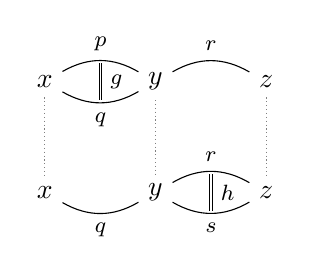
\begin{tikzpicture}[node distance=4em, baseline=(basenode.base)]
        \node[] (x1) {$x$};
        \node[right of=x1] (y1) {$y$};
        \node[right of=y1] (z1) {$z$};
        \node[below of=x1] (x2) {$x$};
        \node[right of=x2] (y2) {$y$};
        \node[right of=y2] (z2) {$z$};
        \draw[bend left] (x1) to node[above] (p) {\footnotesize$p$} (y1);
        \draw[bend right] (x1) to  node[below] (q1) {\footnotesize$q$} (y1);
        \draw[bend left] (y1) to node[above] (r1) {\footnotesize$r$} (z1);
        \draw[bend left] (y2) to node[above] (r2) {\footnotesize$r$} (z2);
        \draw[bend right] (y2) to  node[below] (s) {\footnotesize$s$} (z2);
        \draw[bend right] (x2) to node[below] (q2) {\footnotesize$q$} (y2);
        \draw[double, shorten >=.1em, shorten <=.1em] (p) to node[right] {\footnotesize$g$} (q1);
        \draw[double, shorten >=.1em, shorten <=.1em] (r2) to node[right] {\footnotesize$h$} (s);
        \draw[gray,densely dotted] (x1) to node (basenode){} (x2) (y1) to (y2) (z1) to (z2);
      \end{tikzpicture}%
      =%
      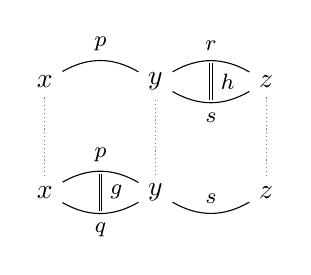
\begin{tikzpicture}[node distance=4em, baseline=(basenode.base)]
        \node[] (x1) {$x$};
        \node[right of=x1] (y1) {$y$};
        \node[right of=y1] (z1) {$z$};
        \node[below of=x1] (x2) {$x$};
        \node[right of=x2] (y2) {$y$};
        \node[right of=y2] (z2) {$z$};
        \draw[bend left] (x2) to node[above] (p) {\footnotesize$p$} (y2);
        \draw[bend right] (x2) to  node[below] (q1) {\footnotesize$q$} (y2);
        \draw[bend right] (y2) to node[above] (r1) {\footnotesize$s$} (z2);
        \draw[bend left] (y1) to node[above] (r2) {\footnotesize$r$} (z1);
        \draw[bend right] (y1) to  node[below] (s) {\footnotesize$s$} (z1);
        \draw[bend left] (x1) to node[above] (p2) {\footnotesize$p$} (y1);
        \draw[double, shorten >=.1em, shorten <=.1em] (p) to node[right] {\footnotesize$g$} (q1);
        \draw[double, shorten >=.1em, shorten <=.1em] (r2) to node[right] {\footnotesize$h$} (s);
        \draw[gray,densely dotted] (x1) to node (basenode){} (x2) (y1) to (y2) (z1) to (z2);
      \end{tikzpicture}%
    \end{sidecaption}
  \end{figure}%
  %
  One prove such a result by induction on $h$. Indeed, when
  $h\jdeq \refl r$, then both sides of the equation reduces through
  path algebra to $\ap {r\cdot\blank} (g)$. Now we are interested in
  this result when $x,y,z$ are all equal to $a$ by definition, and $p,q,r,s$
  are all equal to $\refl a$ by definition. In that case, one has that
  $\ap {\refl a\cdot \blank}$ and $\ap {\blank\cdot\refl a}$ both act
  trivially, and the equation becomes: $h\cdot g = g \cdot h$.

  One still has to prove that the function $\loopspace$ is an inverse
  for $\BB$. Given an abelian group $G$, the proof
  of~\cref{lemma:universal-cover-simply-connected} gives an
  equivalence between $\B\loopspace {(\BB G)}$ and the connected
  component of $\refl {\BG_\div}$ in $\BG_\div\eqto \BG_\div$. By
  definition, this is the classifying type of $\grpcenter(G)$. Being
  abelian, $G$ is isomorphic to its center
  (\cref{def:abelian-groups}), and so it yields an element of
  $\loopspace {(\BB G)} \eqto_{\typegroup} G$. %
  \marginnote[-1.5\baselineskip]{%
    If $X \ptdweto Y$ denote the type of pointed equivalences between
    pointed types $X,Y:\UUp$, then the univalence axiom implies that
    there is an equivalence
    \begin{displaymath}
      (X=Y) \weq (X \ptdweto Y).
    \end{displaymath}%
  }%
  Conversely, take a pointed simply connected $2$-type $(A,a)$. We
  want to produce a pointed equivalence
  $\Phi : (A,a) \equivto \BB (\loopspace {(A,a)}) $. One should first
  notice that the function
  \begin{fullwidth}
    \begin{equation}
      \label{eq:loopspace-A-abelian}%
      \ev^a_{\refl a}{\B\loopspace \left( \BB (\loopspace {(A,a)}) \right)}
      \jdeq \conncomp{((a\eqto a)\eqto (a\eqto a))}{\refl{a\eqto a}} \to (a\eqto a,\refl a).
    \end{equation}
  \end{fullwidth}
  that maps a path
  \begin{displaymath}
    (p,!):(a\eqto a,\settrunc{\refl{a\eqto a}})\eqto (a\eqto a,\settrunc{\refl{a\eqto a}})
  \end{displaymath}
  to the evaluation $p(\refl a): a\eqto a$ is an equivalence, because
  $\loopspace (A,a)$ is an abelian group.

  %% OLD MATERIAL, can still be useful.
  %%
  % We will now provide
  % \begin{displaymath}
  %   \Phi : \BB {(\loopspace {(A,a)})} \ptdto (A,a)
  % \end{displaymath}
  % such that $\loopspace(\Phi)$ is the previous equivalence.
  % To be able to
  % express $\Phi$, we need a small gadget about truncations of
  % function
  % types: for types $X,Y:\UU$, given an element
  % $f_0:\setTrunc{X\to Y}$, one constructs a map
  % $\lceil f_0 \rceil : \setTrunc X \to \setTrunc Y$; the type of
  % $\lceil f_0 \rceil$ being a set, one might as well suppose that
  % $f_0 \jdeq \settrunc f$ for some $f:X\to Y$; then we set
  % $\lceil f_0 \rceil (\settrunc x) = \settrunc{f(x)}$, which
  % suffices
  % in order to define $\lceil f_0 \rceil$ entirely because its
  % codomain
  % $\setTrunc Y$ is a set. If we assume the axiom of
  % choice\footnote{What is the status of AC in this book??}, then
  % $\lceil \blank \rceil$ is injective when $Y$ is a set.
  %%
  We will now define a pointed map
  $\Phi : (A,a) \ptdto \BB (\loopspace {(A,a)})$, and prove
  subsequently that this is an equivalence. Let $T : A \to \UU$ be the
  type family (of sets) define by
  \begin{displaymath}
    T(a') \defequi \sum_{\alpha:\setTrunc{(a\eqto a)\weq(a\eqto a')}}
    \prod_{p:a\eqto a'}\alpha=\settrunc {p\cdot\blank}
  \end{displaymath}
  We claim that $T(a')$ is contractible for all $a':A$. By
  connectedness of $A$, it is equivalent to show that $T(a)$ is
  contractible. However,
  \begin{align*}
    T(a)
    &\jdeq \sum_{\alpha:\setTrunc{(a\eqto a)\equivto(a\eqto a)}}\prod_{p:a\eqto a}
      \alpha = \settrunc {p\cdot \blank}
    \\
    &\weq \sum_{\alpha:\setTrunc{(a\eqto a)\equivto(a\eqto a)}} \alpha = \settrunc{\id_{a=a}}
    \\
    &\weq 1
  \end{align*}
  Then, we define $\Phi (a')$ to be the element
  $(a\eqto a', \kappa_{a'}):\univcover \UU {a\eqto a}$ where
  $\kappa_{a'}$ is the first projection of the center of contraction
  of $T(a')$. In particular, following the chain of equivalences
  above, $\Phi(a)$ is defined as
  $(a\eqto a, \settrunc{\refl {a\eqto a}})$, hence $\Phi(a)$ is
  trivially pointed by a reflexivity path. To verify that $\Phi$, thus
  defined, is an equivalence, one can use connectedness of
  $\BB(\loopspace (A,a))$ and only check that
  $\inv\Phi(a\eqto a,\settrunc{\refl {a\eqto a}})$ is
  contractible. However, there is a canonical equivalence of type:
  \begin{displaymath}
    \inv\Phi(a\eqto a,\settrunc{\refl {a\eqto a}}) \equivto \sum_{a':A}
    \sum_{\varphi : (a\eqto a) \equiv (a\eqto a')}\settrunc{\varphi} = \kappa_{a'}.
  \end{displaymath}
  So we will show that the type on the right hand-side is
  contractible. For an element $a':A$ together with
  $\varphi: (a\eqto a) \equiv (a\eqto a')$ such that the proposition
  $\settrunc \varphi = \kappa_{a'}$ holds, a path between
  $(a,\id_{a\eqto a},!)$ and $(a',\varphi,!)$ consists of a path
  $p:a\eqto a'$ and a path $q:(x\mapsto p x) \eqto \varphi$. We have a
  good candidate for $p$, namely $p\defequi \varphi(\refl
  a):a\eqto a'$. However we don't have quite $q$ yet. Consider, for any
  $a':A$, the function
  \begin{displaymath}
    \ev_{\refl a}^{a'} :
    \left(
      (a\eqto a, \settrunc{\refl{a\eqto a}} ) =
      (a\eqto a', \kappa_{a'} )
    \right)
    \to (a\eqto a')
  \end{displaymath}
  defined as $(\psi,!) \mapsto \psi(\refl a)$.  Note that
  $\ev_{\refl a}^{a}$ is precisely the equivalence
  $\B\loopspace{(\BB\loopspace(A,a))}_\div \equiv (a=a)$ described
  in~\cref{eq:loopspace-A-abelian}. Hence, by connectedness of $A$,
  one gets that the proposition $\isEq(\ev_{\refl a}^{a'})$ holds for
  all $a':A$. In particular, because the propositions
  $\settrunc \varphi = \kappa_{a'}$ and
  $\settrunc {p\cdot\blank} = \kappa_{a'}$ holds, one gets elements
  $(\varphi,!)$ and $(x\mapsto px,!)$ in the domain of
  $\ev_{\refl a}^{a'}$. Their images $\ev_{\refl a}^{a'}(\varphi,!)$
  and $\ev_{\refl a}^{a'}(x\mapsto px,!)$ are both identifiable with
  $p$. By composition, we obtain a path
  $(x\mapsto px,!)\eqto (\varphi,!)$ in the domain. The first
  component provide the path $q:(x\mapsto px) \eqto \varphi$ that we
  wanted.
\end{proof}

\subsection{Higher deloopings}

The function $\BB$ defined in the proof
of~\cref{thm:abelian-groups-weq-sc2types} provides a delooping of
$\BG$ whenever $G$ is abelian. That is, there is an identification
$\loops \BB G \eqto \BG$. A systematic way of obtaining such
deloopings has been developed by David W\"{a}rn\footcite{Warn-EM},
that can be applied here to give an alternative definition of $\BB G$,
and to obtain further deloopings of it.

\begin{definition}[W\"{a}rn]
  Given a pointed type $X$, the type of {\em $X$-torsors} is
  \begin{displaymath}
    TX \defequi \sum_{Y : \UU} \Trunc{Y} \times \left( \prod_{y:Y}(Y,y) \ptdweto X \right).
  \end{displaymath}
  The type of {\em pointed $X$-torsors} is
  $TX_\ast \defequi \sum_{t : TX}\fst t$.
\end{definition}
The usefulness of these definitions in the context of deloopings comes
from the following proposition.
\begin{lemma}[W\"{a}rn]
  Let $X$ be a pointed type. If $TX_\ast$ is contractible, then for
  any pointed $X$-torsors $(t,y)$, the pointed type $(TX,t)$ is a
  delooping of $X$.
\end{lemma}
\begin{proof}
  Suppose $(t,y)$ is a center of contraction for $TX_\ast$. By
  contracting away (\cref{lem:contract-away}) in two different ways,
  we obtained a composition of equivalences:
  \begin{displaymath}
    (t \eqto t) \equivto \sum_{u : TX}\fst u \times (t \eqto u) \equivto \fst t 
  \end{displaymath}
  that maps $\refl t$ to $y$. In other words, this equivalence,
  trivially pointed, presents $(TX, t)$ as a delooping of
  $(\fst t, y)$. Moreover, the $X$-torsor $t$ comes by definition with
  an identification $(\fst t,y) \ptdweto X$. So in the end, we have an
  equivalence $(TX, t) \ptdweto X$.
\end{proof}

\begin{xca}\label{xca:sections-as-dependent-functions}
  Recall that a \emph{section} (see~\cref{def:surjection} and its
  accompanying footnote) of a function $f:A \to B$ is a function
  $s: B \to A$ together with an identification $f\circ s \eqto \id_B$.
  Construct an equivalence from the type $\secfun f$ of sections of
  $f$ to the type $\prod_{b:B}\sum_{a:A}b \eqto f(a)$.
\end{xca}

Consider the evaluation function
$\ev_{X_\div,Y} : (X_\div \eqto Y) \to Y$ (defined by path-induction,
sending $\refl X$ to the distinguished point of $X$). In other words,
the function $\ev_{X_\div,Y}$ takes an identification of $X_\div$ with
$Y$ and returns the point in $Y$ corresponding to the distinguished
point of $X$ under this identification.  Applying
\cref{xca:sections-as-dependent-functions} to $\ev_{X_\div,Y}$ we get
an equivalence of type
\begin{displaymath}
  TX \equivto \sum_{Y : \UU} \Trunc{Y} \times \secfun(\ev_{X_\div,Y}).
\end{displaymath}
This alternative description of the type of $X$-torsors is the key
ingredient to compare W\"arn's delooping of the classifying type of
an abelian group with our.

\begin{lemma}\label{lem:warn-abelian-group}
  For any abelian group $G$, the type $T(\BG)$ can be identified with
  $\BB G$.
\end{lemma}
\begin{proof}
  Let $G$ be an abelian group. We first construct, for each type
  $Y$, a function
  $f_Y : \Trunc{Y} \times \secfun(\ev_{\BG_\div,Y}) \to
  \setTrunc{\BG_\div \eqto Y}$, and then prove that $f_Y$ is an
  equivalence. Given a type $Y$ and an element
  $(!,s) : \Trunc{Y} \times \secfun(\ev_{X_\div,Y})$, we can easily
  prove that $Y$ is connected: being connected is a proposition, so
  we can assume that we have an actual $y:Y$ and then
  $s(y) : \BG_\div \eqto Y$ proves that $Y$ is as connected as
  $\BG_\div$ is. Consequently $s$ must send $Y$ into one of the
  connected component of $\BG_\div \eqto Y$, that we choose to be
  $f_Y(!,s)$. With this definition, the fiber of $f_Y$ at any given
  $c : \setTrunc{\BG_\div \eqto Y}$ can be identified with the type
  of sections $s$ of $\ev_{\BG_\div,Y}$ with values in $c$. However,
  for any $Z$ and $p: \BG_\div \eqto Z$ the restriction of the
  evaluation
  $\ev_{\BG_\div,Z}\restriction_p : \conncomp{(\BG_\div \eqto Z)} p
  \to Z$ is an equivalence: indeed, by induction, we only have to
  show it for $p\jdeq \refl {\BG_\div}$, in which case
  $\ev_{\BG_\div,\BG_\div}\restriction_{\refl {\BG_\div}}$ is
  exactly the map $\B\grpcenterinc G$ defined in
  \cref{sec:center-group}, which is an equivalence since $G$ is
  abelian by \cref{def:abelian-groups}. Thus, given any $p$, the
  fiber of $f_Y$ at $\settrunc p$ is contractible. Being
  contractible is a proposition, hence a set, so it follows that the
  fiber of $f_Y$ at any $c:\setTrunc{\BG_\div \eqto Y}$ is
  contractible. In other words, $f_Y$ is an equivalence, as
  announced. We have thus a chain of equivalences:\footnote{Notice
    that the construction of an equivalence
    $TX \equivto \univcover \UU {X_\div}$ that we carried for
    $X\jdeq\BG$ relies only on $X_\div$ being connected and
    $\ev_{X_\div,X_\div}\restriction_{\refl {X_\div}}$ being an
    equivalence. Such types $X$ are called \emph{central} and are
    studied in details by~\citeauthor{BCFR}\footnotemark{}.}.%
  \footcitetext{BCFR}
  \begin{displaymath}
    T(\BG) \equivto \sum_{Y : \UU} \Trunc{Y} \times \secfun(\ev_{X_\div,Y})
    \equivto \sum_{Y : \UU} \setTrunc{\BG_\div \eqto Y} \jdeq \BB G
  \end{displaymath}
\end{proof}

Notice that where W\"arn's method shines, compared to our, is in
producing further delooping $\B^n G$ for $n\geq 3$.

\section{Direct sums and reduced wreath products}
\label{sec:direct-sums}

Sketch:
We saw in~\cref{sec:coprod} how to produce sums of groups,
and noticed that a sum of abelian groups is rarely abelian.
Indeed, the free group on two generators $\FG_2$
is the sum of two copies of $\ZZ$.

But a very similar construction works to produce sums of \emph{abelian groups}.

\begin{example}[Lamplighter group]
  $\CG_2 \mathbin{\wr} \ZZ$
  \wip{Wait: how do we do infinite direct sums in general?}
\end{example}

\section{Stabilization}

%%% Local Variables:
%%% mode: LaTeX
%%% fill-column: 144
%%% latex-block-names: ("lemma" "theorem" "remark" "definition" "corollary" "fact" "properties" "conjecture" "proof" "question" "proposition" "exercise")
%%% TeX-master: "book"
%%% TeX-command-extra-options: "-fmt=macros"
%%% compile-command: "make book.pdf"
%%% End:

\chapter{Rings, fields and vector spaces}
\label{ch:fields}

In this chapter we will extend the hierarchy of algebraic structures from 
monoids (\cref{def:monoid}) and 
groups (\cref{def:typegroup}) to
rings (\cref{def:abstractring}),
fields (\cref{def:field}), and
vector spaces (\cref{def:vectorspace}).
Of all these structures there are several varieties, 
satisfying additional properties, such as 
abelian groups (\cref{sec:abelian-groups}),
non-trivial rings (\cref{def:non-trivial-ring}),
commutative rings (\cref{def:commutative-ring}),
....

Quotients; subspaces (= ?). Bases and so. Dual space; orthogonality. (all of this depends on good implementations of subobjects). Eigen-stuff. Characteristic polynomials; Hamilton-Cayley.

\section{Rings, abstract and concrete}\label{sec:rings}

A ring is an algebraic structure that consists of a group and a
monoid that share the same underlying set. The interaction between
the respective operations is governed by laws that are called
the distributivity laws. 
The standard example of a (commutative) ring 
is the ring with set of integers as underlying set, with addition as
group operation and multiplication as monoid operation.
Note that multiplication in a ring need not be commutative.\footnote{%
In contrast, in \cref{xca:ring-group-abelian} you are asked to prove
that the group of a ring is always abelian, as a consequence of the
extra structure and properties.} We start by defining rings abstractly.

\subsection{Abstract rings}\label{sec:abstrings}

We follow the convention that the group data of an abstract group
are denoted by $0,\,+,\,-$ and the monoid data by $1,\,\cdot\,$.

\begin{definition}\label{def:abstractring}
An \emph{abstract ring} $\mathscr R$ consists of an abstract group 
$(R,0,+,-)$ and a monoid $(R,1,\cdot)$ with the
same underlying set $R$. Moreover, the following equations should hold
for all $a,b,c : R$:
    \begin{enumerate}      %[ref=\ref{def:abstractring} (\alph*)]
    \item\label{ring:ldistr-law} $a \cdot (b + c) = a \cdot b + a \cdot c$ (the \emph{left distributive law})
    \item\label{ring:rdistr-law} $(a + b) \cdot  c = a \cdot c + b \cdot c$ (the \emph{right distributive law})
    \end{enumerate}
The latter two properties
are together denoted by $\mathrm{DistrLaws}(R,\cdot,+)$.

The abstract ring $\mathscr R$ is called \emph{non-trivial} if $0\neq 1$
and \emph{commutative} if its multiplication $\cdot$ is commutative, that is,
if $a\cdot b= b\cdot a$ for all $a,b:R$.
\end{definition}

The abstract group $(R,0,+,-)$ is called the \emph{(additive) group}
of $\mathscr R$, and the monoid $(R,1,\cdot)$ the 
\emph{(multiplicative) monoid} of $\mathscr R$.

\begin{definition}\label{def:typering}
The type of abstract rings is defined as\footnote{%
See \cref{not:GroupLaws} for the monoid laws.}
\begin{align*}
\typering\defeq 
\sum_{(R,0,+,-):\Group^{\abstr}} ~ &\sum_{e:R} ~ \sum_{\mu:R\to R\to R} \\
&\mathrm{MonoidLaws}(R,e,\mu)\times\mathrm{DistrLaws}(R,\mu,+).
\end{align*}
The type $\typecommring$ of commutative rings is similar to the type
of rings with the additional property $\prod_{a,b:R}\mu(a,b)=\mu(b,a)$. 
\end{definition}

\begin{xca}\label{xca:ring-group-abelian}
Let $\mathscr R$ be an abstract ring. Show that the additive group 
of $\mathscr R$ is abelian. Hint: elaborate $(a+1)\cdot(b+1)$.
\end{xca}

\begin{definition}\label{def:ringhom}
Let $\mathscr R,\mathscr S : \Ring$ be abstract rings, with
$\mathscr R$ consisting of an abstract group $\agp R$ with underlying set $R$
and a monoid $(R,1_R,\cdot_R)$, and 
$\mathscr S$ consisting of an abstract group $\agp S$ with underlying set $S$
and a monoid $(S,1_S,\cdot_S)$.
An \emph{abstract ring homomorphism} from $\mathscr R$ to $\mathscr S$ is an
abstract homomorphism $f:\absHom(\agp R,\agp S)$ that is a monoid homomorphism
from $(R,1_R,\cdot_R)$ to $(S,1_S,\cdot_S)$.
\end{definition}



\begin{example}\label{exa:ring-Z-polynomials}
We elaborate the abstract ring of polynomials with integer coefficients.
\MB{TBD}
\end{example}

\subsection{Mixed rings}\label{sec:mixring}

Here we explore a definition of a ring that is based
on a concrete group $G$ and left and right multiplications 
that are still half abstract. %Therefore we call them mixed rings.

We first note that, for any abstract ring $\mathscr R$ and elements $a,b:R$,
the left multiplication function $(a\cdot\blank)$ 
and the right multiplication function $(\blank\cdot b)$ are
abstract homomorphisms
of the additive group $(R,0,+,-)$ of $\mathscr R$ to itself.\footnote{%
    These functions provide two ways to write the product $a\cdot b$,
see the coherence law in \cref{def:mixring}\ref{mixring:lr-coherence-law}.}
There are two ways to compose them: $(a\cdot(\blank\cdot b))$
and $((a\cdot\blank)\cdot b)$. Equality of the latter two functions is
an elegant way of expressing associativity.
These observations lead to the following alternative definition of a ring.

\begin{definition}\label{def:mixring}
An \emph{mixed ring} $R$ consists of a group\footnote{%
It will follow as in \cref{xca:ring-group-abelian} that the group $R$
is abelian.} also denoted $R$ together with
a symmetry $1_R : \USymR$ and two maps $\ell,r: \USymR\to\Hom(R,R)$
from the set of symmetries in $R$ to the set of homomorphisms from
$R$ to $R$.\footnote{We call these rings ``mixed'' since they are
based on a concrete group $R$ and data referring to $\abstr(R)$.}
Given $g:\USymR$, we write $\ell_g$ for the homomorphism $\ell(g)$ and 
$r_g$ for $r(g)$.
Moreover, the following equations should hold.
    \begin{enumerate}
    \item\label{mixring:unit-laws} $\ell_{1_R} = \id_G = r_{1_R}$ (the \emph{multiplicative unit laws})
    \item\label{mixring:lr-coherence-law} $(\USym\ell_g)(h) = (\USymr_h)(g)$, 
    for all $g,h : \USymR$ (the \emph{coherence law})
        \item\label{mixring:assoc-law} $\ell\circ r= r\circ\ell$ (the \emph{associativity law})
    \end{enumerate}
%The properties \ref{mixring:unit-laws}-\ref{mixring:assoc-law} 
%are together denoted by $\RingProps(R,1_R,\ell,r)$.
The ring $R$ is called \emph{commutative} if $\ell=r$,
and \emph{non-trivial} if $1_R \neq \refl{R}$.
\end{definition}

The coherence law \ref{mixring:lr-coherence-law} allows us to abbreviate both 
$(\USym\ell_g)(h)$ and $(\USymr_h)(g)$ by $g\cdot h$. We will do this when
no confusion can occur. Then, $\ell=r$ 
amounts to $g\cdot h = h\cdot g$, for all $g,h : \USymG$,
as could be expected from the abstract case.

We proceed by giving the standard example of the integers as a ring
in the sense of \cref{def:mixring}.
\begin{example}
Consider the group $\ZZ$ classified by the circle.
Using the same notation $\ZZ$ also for the ring, take $1_\ZZ \defeq\Sloop$
and $\ell: (\base\eqto\base)\to\Hom(\ZZ,\ZZ)$ defined as follows.
For every $g:\base\eqto\base$, let $\ell_g$ be the homomorphism
classified by the map $\B\ell_g(\base)\defeq\base$, 
$\B\ell_g(\Sloop)\defis g$, and pointed by reflexivity.\footnote{%
The reader may recognize the degree $m$
map from \cref{def:mfoldS1cover} as a special case.}
Take $r\defeq\ell$. Now the unit laws, the coherence law and
the associativity law can easily be verified. It follows that
$(\ZZ,1_\ZZ,\ell,!)$ is a non-trivial commutative ring.
\end{example}

\begin{definition}\label{def:typemixring}
The type of rings is defined as
\[
\typering\defeq\sum_{R:\typegroup}\sum_{1_R:\USymR}\sum_{\ell,r:\USymR\to\Hom(R,R)} \RingProps(R,1_R,\ell,r).
\]
The type $\typecommring$ of commutative rings is similar to the type
of rings but with $\RingProps(R,1_R,\ell,r) \times(\ell=r)$. 
\end{definition}
% end wip

\begin{xca}\label{xca:Rmixring->URabstring}
Let $(R,1_r,\ell,r)$ be an mixed ring. 
Show that $\USymR$ is an abstract ring with
additive group $\abstr(R)$ and multiplicative 
monoid $(\USymR,1_R,\cdot)$. \MB{TBD}
\end{xca}

\subsection{Move to a better place (Ch.\ 11 or 2)}
\begin{marginfigure}
  \begin{tikzcd}[ampersand replacement=\&,column sep=small]
  \pt_Y\ar[rr,eqr,"f_\pt"]\ar[ddrr,eql,"g_\pt"']
  \& \& f(\pt_X)  \ar[dd,eqr,"k(\pt_X)"]
  \\ \& \mbox{} \& \\
  \pt_Y\ar[uu,"{\jdeq}"']\ar[rr,eql,"g_\pt"']\ar[ddrr,eql,"h_\pt"']    
  \& \mbox{} \& g(\pt_X)\ar[dd,eqr,"k'(\pt_X)"]
  \\\& \mbox{} \& \\
 \&\& h(\pt_X)
  \end{tikzcd}
  \caption{\label{fig:ptd-homotopy-compo}
  Path for $(k'\cdot_{\protect\ptw} k)$.} 
\end{marginfigure}
\begin{definition}\label{def:ptd-homotopy-compo}
Let $X$ and $Y$ be pointed types and
$f,g: X\ptdto Y$ pointed maps from $X$ to $Y$.
Recall from \cref{con:identity-ptd-maps} the equivalence $\ptw_*$ of type 
$(f\eqto g) \equivto H(f,g)$, where 
\[ H(f,g) \defeq \sum_{k:\prod_{x:X}(f_\div(x)\eqto g_\div(x))}
                               ((k(\pt_X)\cdot f_\pt) \eqto g_\pt ).
\]

Assume also $h: X\ptdto Y$ and let $k: H(f,g)$ and 
$k': H(g,h)$. In line with the notation for pointed maps, 
we denote the pair $k$ by $(k_\div,k_\pt)$, an likewise for $k'$. 
Define the \emph{pointwise composition}
$(k'\cdot_{\ptw} k)$ of $k'$ and $k$ by\footnote{%
We use $k_\div$ to denote the first component of $k$,
as we do for non-dependent pointed maps, but we will often drop
this subscript ``$\div$''.
We use the notation ``$\cdot_{\ptw}$'' for pointwise composition
of $k$ and $k'$, as well as of $k_\div$ and $k'_\div$.}
\begin{align*}
\bigl(k'\cdot_{\ptw} k\bigr)&\defeq
\bigl(k'_\div\cdot_{\ptw} k_\div ~,~ 
       k'_\pt\cdot\ap{(k'_\div(\pt_X)\cdot\blank)}(k_\pt)\bigr),
\quad\text{where}\\
(k'_\div\cdot_{\ptw} k_\div) &\defeq (x\mapsto k'_\div(x)\cdot k_\div(x)).
\end{align*}
In \cref{fig:ptd-homotopy-compo}, the upper-right triangle represents
the type of $k_\pt$, the upper-left triangle is a reflexivity triangle,
the lower triangle represents the type of $k'_\pt$,
and the outer diagram represents the type 
$k'(\pt_X)\cdot k(\pt_X)\cdot f_\pt \eqto h_\pt$
of $k'_\pt\cdot\ap{(k'_\div(\pt_X)\cdot\blank)}(k_\pt)$.
Thus we see that $(k'\cdot_{\ptw} k)$ is an element of $H(f,h)$.
\end{definition}

\begin{construction}\label{con:ptd-homotopy-compo}
Let conditions be as in \cref{def:ptd-homotopy-compo}.
Let $p:(f\eqto g)$ and $q:(g\eqto h)$.
Then we have an identification of $\ptw_*(qp)$ with
$\ptw_*(q) \cdot_{\ptw} \ptw_*(p)$.
\end{construction}
\begin{implementation}{con:ptd-homotopy-compo}
By path induction on $q$, it suffices to construct an identification
of $\ptw_*(p)$ and $\ptw_*(\refl{g}) \cdot_{\ptw} \ptw_*(p)$.
Using \cref{con:identity-ptd-maps} and \cref{def:funext} we
can identify $\ptw_*(\refl{g})$ with the pair
$((x\mapsto\refl{g_\div(x)}),\refl{g_\pt)}$. 
For use in \cref{fig:ptd-homotopy-compo} we write the latter
pair as $(k'_\div,k'_\pt)$, noting that $h\jdeq g$ in this case.
Writing also $(k_\div,k_\pt)$ for $\ptw_*(p)$, the goal is to
identify $(k'\cdot_{\ptw} k)$ with $k$.
This identification is easily obtained by using
that $\refl{g(x)}\cdot r$ is definitionally equal to $r$,
for all $x:X$ and $r:f(x)\eqto g(x)$.
\end{implementation}

\begin{definition}\label{def:cst-ptd}
Let $A$ and $B$ be pointed types.
For any $b:B$ and $p:\pt_B\eqto b$, 
define the \emph{pointed constant map} $\cst{\ast}^A(b,p) : A\ptdto B$
\emph{at} $(b,p)$ by setting $\cst{\ast}^A(b,p)\defeq (\cst{b}^A,p)$.\footnote{%
Here $\cst{b}^A$ is from \cref{def:cst-map}.
We may omit superscripts $A$ if $A$ is clear from the context.}
Thus $\cst{\ast}^A$ is a function from $\sum_{x:B}(\pt_B\eqto x)$ to
$A\ptdto B$.\footnote{%
Of course, $\sum_{x:B}(\pt_B\eqto x)$ is contractible.
In \cref{def:O-functor} we will see why $\cst{\ast}^A$ is useful.}
\end{definition}

\begin{remark}\label{rem:loops-at-cst-ptd}
In case $f$ and $g$ in \cref{def:ptd-homotopy-compo} are both the point of
$X\ptdto Y$, \ie $f\jdeq g\jdeq\pt_{X\ptdto Y}\jdeq(\cst{\pt_Y},\refl{\pt_Y})$,
it is an advantage to work with a minor variant of $\ptw_*$ of type 
$\loops({X\ptdto Y}) \equivto (X\ptdto\loops Y)$.
The latter type is obtained by definitional simplifications
and replacing $(h(\pt_X)\cdot \refl{\pt_Y})\eqto \refl{\pt_Y}$
in $H(\pt_{X\ptdto Y},\pt_{X\ptdto Y})$ 
by an equivalent type:\footnote{By laws of symmetry and right unit.}
\[ H(\pt_{X\ptdto Y},\pt_{X\ptdto Y}) \equivto 
\sum_{h:X\to\loops Y}(\refl{\pt_Y}\eqto h(\pt_X)) \jdeq
(X\ptdto\loops Y).
\]
Abusing notations, we denote this variant also by $\ptw_*$.
\end{remark}


The following construction is useful since it
will allow us to simplify identifying two pointed maps
to identifying their underlying unpointed maps
in some important cases. The construction is based on BCFR which
in turn uses a result by Cavallo.

\begin{construction}\label{con:Id-(B->*A)}
Let $A$ be a pointed type and let $\ev: (\id_A\eqto\id_A)\to(\pt_A\eqto\pt_A)$
be the evaluation map that sends identifications $i:(\id_A\eqto\id_A)$ 
to paths $\ptw(i)(\pt_A) : (\pt_A\eqto\pt_A)$.
Furthermore, let  $s: (\pt_A\eqto\pt_A)\to(\id_A\eqto\id_A)$
be a section of $\ev$, that is, we are given
identifications $\ev(s(p))\eqto p$ for all $p:(\pt_A\eqto\pt_A)$.
Let also $B$ be a pointed type and consider pointed
maps $f,f' : B\ptdto A$ with underlying unpointed maps
$f_\div,f'_\div : B\to A$.

Then we have a map $(f_\div\eqto f'_\div)\to(f\eqto f')$.
\end{construction}

\begin{implementation}{con:Id-(B->*A)}
By path induction on $f_\div\eqto f'_\div$ we may take
$f_\div\jdeq f'_\div$, so that the goal is to identify\footnote{%
Henceforth we simply write $f$ for $f_\div$.}
$(f,f_\pt)$ with $(f,f'_\pt)$, 
for two paths $f_\pt,f'_\pt: (\pt_A\eqto f(\pt_B))$.

Define $r\defeq (f'_\pt\cdot\inv{f}_\pt) : (f(\pt_B)\eqto f(\pt_B))$.
By \cref{con:identity-ptd-maps}, it suffices to give
an element $h: \prod_{b:B}(f(b)\eqto f(b))$ and an identification
of $h(\pt_B)$ with $r$.
By path induction on $f_\pt$ we may take $\pt_A\jdeq f(\pt_B)$,
so that the domain of $s$ is $f(\pt_B)\eqto f(\pt_B)$,
and so $r$ is an element of this domain. 
Now take $h(b)\defeq \ptw(s(r))(f(b))$ for any $b:B$.
Then indeed $h(b):(f(b)\eqto f(b))$, and we can identify
$h(\pt_B)\jdeq \ptw(s(r))(f(\pt_B))\jdeq\ev(s(r))$ with $r$ 
since $s$ is a section of $\ev$.
\end{implementation}

\begin{construction}\label{con:ev-section-loopsA}
Let $A$ be a pointed type and $\loops A$ its pointed loop type.
We use $\pt$ for $\pt_A$ and $\rfl$ for $\refl{\pt_A}$.
Let $\ev: (\id_{\loops A}\eqto\id_{\loops A})\to (\rfl\eqto\rfl)$ 
be the evaluation map that sends $i:(\id_{\loops A}\eqto\id_{\loops A})$
to $\ptw(i)(\rfl)$. 
Then $\ev$ has a section, that is, a 
map $s: (\rfl\eqto\rfl)\to(\id_{\loops A}\eqto\id_{\loops A})$
with identifications $\ev(s(\alpha))\eqto\alpha$ for 
all $\alpha: (\rfl\eqto\rfl)$.
\end{construction}

\begin{implementation}{con:ev-section-loopsA}
Recall from \cref{def:funext} the equivalence $\ptw$ identifying
$\id_{\loops A}\eqto\id_{\loops A}$ with $\prod_{p:\loops A}(p\eqto p)$.
Since $(\rfl\cdot p)$ and $p$ are definitionally equal for any $p:\loops A$,
any $\alpha: (\rfl\eqto\rfl)$ gives a path 
$\ap{\blank\cdot p}(\alpha): (p\eqto p)$.\footnote{%
In a picture:
\[
  \begin{tikzcd}[ampersand replacement=\&,column sep=large]
  \rfl \ar[r,mapsto,"{\blank\cdot p}"]\ar[d,eql,"\alpha"']
  \& (\rfl\cdot p)  \ar[d,eqr,shift right=1em,"{\ap{\blank\cdot p}(\alpha)}"] \jdeq p
\\
  \rfl \ar[r,mapsto,"{\blank\cdot p}"]
  \& (\rfl\cdot p) \jdeq p
  \end{tikzcd}
\]
}
Taking $\rfl$ for $p$, $\ap{\blank\cdot \rfl}(\alpha)$
can be identified with $\alpha$.\footnote{%
As obvious as this may seem, it requires a generalization of
the type of $\alpha$ to enable path induction, and we delegate
this to \cref{xca:ev-section-loopsA}.} 
For any $\alpha: (\rfl\eqto\rfl)$ and $p:\loops A$,
define $s_\alpha$ by $s_\alpha(p)\defeq\ap{\blank\cdot p}(\alpha)$.
Then $\inv{\ptw}(s_\alpha):(\id_{\loops A}\eqto\id_{\loops A})$.
Hence 
\[
s\defeq(\alpha\mapsto\inv{\ptw}(s_\alpha)) : 
(\rfl\eqto\rfl)\to(\id_{\loops A}\eqto\id_{\loops A}),
\]
and we have 
$\ev(s(\alpha)) \jdeq \ptw(\inv{\ptw}(s_\alpha))(\rfl) \eqto \alpha$ 
by \cref{def:funext} and \cref{xca:ev-section-loopsA}.
\end{implementation}

\begin{exercise}\label{xca:ev-section-loopsA}
Given a type $A$ with elements $a,x:A$ and a path $q:a\eqto x$,
define $\rho_{q} : (q\cdot\refl{a}) \eqto q$ by induction on $q$.
For any $p:a\eqto a$ and $\beta:(p\eqto \refl{a})$,
define $i(\beta): \ap{\blank\cdot\refl{a}}(\beta) \eqto
\beta\cdot\rho_{p} $ by induction on $\beta$.
Now, give an identification of $\ap{\blank\cdot\refl{a}}(\alpha)$ and 
$\alpha$ for any $\alpha:(\refl{a}\eqto \refl{a})$.
\end{exercise}

\begin{corollary}\label{cor:Id-(B->*loopsA)}
The combination of \cref{con:Id-(B->*A)} and \cref{con:ev-section-loopsA}
yields a function from $(f_\div\eqto f'_\div)$ to $(f\eqto f')$ for all pointed
maps $f,f' : B\ptdto \loops A$.
\end{corollary}

Recall $\loops$ from \cref{def:looptype} and \cref{def:loops-map},
which together form a wild functor $\UUp\to\UUp$, \cf \cref{sec:naturality}. 
In the following we will define a closely related
wild functor that is sometimes easier to use.

\begin{definition}\label{def:O-functor}
For any pointed type $A$, define $\OO A \defeq (\Sc\ptdto A)$.
Let $A$ and $B$ be pointed types and let $f: A\ptdto B$ be a pointed map.
Define $\OO(f):\OO A\ptdto \OO B$ to be composition with $f$,
that is, for $g:(\Sc\ptdto A)$, $\OO(f)(g)\defeq(f\circ g):(\Sc\ptdto B)$.%
\footnote{Here we mean composition as pointed maps,
so that the pointing path $\OO(f)(g)_\pt$ is defined in 
\cref{def:pointedtypes} as $f(g_\pt)\cdot f_\pt$.}
We point $\OO(f)$ as follows. First, observe that
$\pt_{\OO B}\jdeq\pt_{\Sc\ptdto B}\jdeq(\cst{\pt_B},\refl{\pt_B})$ and
$\OO(\pt_{\OO A})\jdeq f\circ\pt_{\OO A}\jdeq (\cst{f(\pt_A)},f_\pt)$.
So both $\pt_{\OO B}$ and $\OO(\pt_{\OO A})$ are images of
$\cst{\ast}^\Sc$, and we can obtain a path between them 
by applying $\cst{\ast}^\Sc$ to the unique path $(f_\pt,\rho_{f_\pt})$
between $(\pt_B,\refl{\pt_B})$ and $(f(\pt_A),f_\pt)$ 
in the contractible type $\sum_{x:B}(\pt_B\eqto x)$.\footnote{%
Here $\rho_{f_\pt} : f_\pt \cdot \refl{\pt_B} \eqto f_\pt$
is defined by induction on $f_\pt$, 
setting $\rho_{\refl{\pt_B}}\defeq\refl{\refl{\pt_B}}$.
}
The situation is illustrated in the diagram below and we define 
$\OO(f)_\pt\defeq\ap{\cst{\ast}}(f_\pt,\rho_{f_\pt})$.
\end{definition}
\[
\begin{tikzcd}[ampersand replacement=\&,column sep=small]
   (\pt_B,\refl{\pt_B})
    \ar[r,mapsto,"{\cst{\ast}}"]
    \ar[d,eql,"{(f_\pt,\rho_{f_\pt})}"']
  \& (\cst{\pt_B},\refl{\pt_B})\jdeq\pt_{\OO B}
    \ar[d,eqr,"{\ap{\cst{\ast}}(f_\pt,\rho_{f_\pt})}"]
\\
  (f(\pt_A),f_\pt)
    \ar[r,mapsto,"{\cst{\ast}}"] 
  \& (\cst{f(\pt_A)},f_\pt)\jdeq\OO(\pt_{\OO A})
  \end{tikzcd}
\]
Note that $\OO(f)_\pt$ is a reflexivity path if $f_\pt\jdeq\refl{\pt_B}$.
\begin{xca}\label{xca:O-functor}
Complete the structure of $\OO$ as a wild functor, \cf \cref{sec:naturality}.
Identify $\OO(f)_\pt$ with $\inv{\ptw_*}(\cst{f_\pt},\rho_{f_\pt})$.
\end{xca}


\begin{remark}\label{rem:pointing-ev}
Given a pointed type $A$, recall from \cref{cor:circle-loopspace}
the equivalence $\ev_A$ from $\Sc\ptdto A$ to $\loops{A}$.
This equivalence sends $f:\Sc\ptdto A$ to $\loops(f)(\Sloop)\jdeq
\inv{f_\pt}\cdot f(\Sloop)\cdot f_\pt$, and the
inverse $\inv{\ev}_A$ sends $p:\loops{A}$ to the pointed map
$f:\Sc\ptdto A$ defined by  $f(\base)\defeq\pt_A$ and $f(\Sloop)\defis p$,
pointed by reflexivity.\footnote{When $A$ is clear from the context 
we may simply write $\ev$. Similarly for $\varepsilon_A$ defined next.}

The equivalence $\ev_A$ can itself be
pointed as follows. The point of $\Sc\ptdto A$ is the constant map 
$\cst{\pt_A}$, pointed by reflexivity, which is sent by $\ev_A$ 
to $\cst{\pt_A}(\Sloop)\cdot \refl{\pt_A}$.\footnote{%
Recall that reflexivity paths cancel definitionally on the left.} Define 
$\varepsilon_A(p): \refl{\pt_A} \eqto (\cst{\pt_A}(p)\cdot\refl{\pt_A})$,
for any $z:\Sc$, $p:\base\eqto z$, by path induction, setting
$\varepsilon_A(\refl{\base})\defeq \refl{\refl{\pt_A}}$.\footnote{%
Note that $\cst{\pt_A}(p):\loops A$ for any $p$.} 
Now we define $(\ev_A)_\pt \defeq \varepsilon_A(\Sloop)$.
\end{remark}

The following construction shows that $\loops$
corresponds to $\OO$ from \cref{def:O-functor} under the equivalences $\ev$,
as illustrated in \cref{fig:Omega-O}.\footnote{\MB{$\ev_\blank$ is an example
of a wild natural equivalence between the wild functors
$\loops, \Sc\blank : \UUp\ptdto\UUp$, cf.\ \cref{ch:cats}.}}


\begin{marginfigure}
  \begin{tikzcd}[ampersand replacement=\&,column sep=small]
  \OO A\ar[rr,"\OO(f)"]\ar[dd,equivl,"\ev_A"']
  \& \&\OO B  \ar[dd,equivr,"\ev_B"]
  \\ \& \mbox{} \& \\
  \loops{A}\ar[rr,"\loops(f)"'] \& \& \loops{B}
  \end{tikzcd}
  \caption{\label{fig:Omega-O} $\loops(f)$ and $\protect\OO(f)$ correspond.} 
\end{marginfigure}


\begin{construction}\label{con:Omega-O}
Let $A$ and $B$ be pointed types and 
let $f: A\ptdto B$ be a pointed map.
Then we have an identification of $\loops(f)\circ \ev_A$ 
and ${\ev_B} \circ {\OO(f)}$, as represented by \cref{fig:Omega-O}.
Consequently, we have that $e\defeq(\inv{\ev_B}\circ{{\blank}\circ\ev_A})$
is an equivalence of type 
$(\loops A\ptdto\loops B)\equivto(\OO A\ptdto\OO B)$,
and $\OO \eqto (e\circ \loops)$. 
\end{construction}

\begin{figure}
  \begin{tikzcd}[ampersand replacement=\&,column sep=small]
  (\Sc\ptdto A)\ar[rr,"\ev_A"]
  \& \& \loops A \ar[rr,"{\loops(f)}"]
  \& \& \loops B 
  \\ 
  (p,p_\pt)\ar[rr,mapsto]
  \& \& \inv{p_\pt}\cdot p(\Sloop)\cdot p_\pt \ar[rr,mapsto]
  \& \& \inv{f_\pt}\cdot f(\inv{p_\pt}\cdot p(\Sloop)\cdot p_\pt)\cdot f_\pt
   \quad (1)
  \\
  (\Sc\ptdto A)\ar[rr,"\OO(f)"]
  \& \& (\Sc\ptdto B) \ar[rr,"{\ev_B}"]
  \& \& \loops B
  \\ 
  (p,p_\pt)\ar[rr,mapsto]
  \& \& (f\circ p,f(p_\pt)\cdot f_\pt) \ar[rr,mapsto]
  \& \& \inv{(f(p_\pt)\cdot f_\pt)}\cdot (f\circ p)(\Sloop)
  \cdot (f(p_\pt)\cdot f_\pt)  \quad (2)
  \end{tikzcd}
  \caption{\label{fig:Omega-O-elab} 
  Elaborating the two composites $(\Sc\ptdto A)\to\loops B$.} 
\end{figure}


\begin{implementation}{con:Omega-O}
We will apply \cref{con:identity-ptd-maps}.
Elaborating the situation in \cref{fig:Omega-O-elab}, we have to identify
$(1)\jdeq \inv{f_\pt}\cdot f(\inv{p_\pt}\cdot p(\Sloop)\cdot p_\pt)\cdot f_\pt$
and $(2)\jdeq \inv{(f(p_\pt)\cdot f_\pt)}\cdot (f\circ p)(\Sloop)
\cdot (f(p_\pt)\cdot f_\pt)$ by a path $i(f,f_\pt)(p,p_\pt)$, 
for all $(p,p_\pt)$.\footnote{We often leave out the ``$\ap{\blank}$'s''.}
Moreover, we must fill the following triangle:
\[
\begin{tikzcd}[ampersand replacement=\&,row sep=tiny]
  \& \&\inv{f_\pt}\cdot f(\cst{\pt_A}(\Sloop)\cdot \refl{\pt_A})\cdot f_\pt  \ar[dddd,eqr,"{i(f,f_\pt)(\cst{\pt_A},\refl{\pt_A})}"]
\\
  \&\inv{f_\pt}\cdot f_\pt
   \ar[ru,eqr,"{\loops(f)((\ev_A)_\pt)}"]
\\
  \refl{\pt_B}
  \ar[rd,eql,"{(\ev_B)_\pt}"'] 
  \ar[ru,eqr,"{\loops(f)_{\pt}}"]
\\
 \&\cst{\pt_B}(\Sloop)\cdot\refl{\pt_B}
    \ar[rd,eql,"{\ev_B(\OO(f)_\pt)}"']  
\\
 \& \&\inv{f_\pt}\cdot \cst{f(\pt_A)}(\Sloop)\cdot f_\pt 
\end{tikzcd}
\]
For defining $i(f)(p,p_\pt)$ we apply path induction on $p_\pt$ and on $f_\pt$,
setting $\pt_A\jdeq p(\base)$ and $p_\pt\jdeq \refl{p(\base)}$,
as well as  $\pt_B\jdeq f(\pt_A)\jdeq f(p(\base))$ and
$f_\pt\jdeq \refl{f(p(\base))}$. Then identifying (1) and (2)
reduces to the task of identifying 
$f(p(\Sloop)\cdot \refl{p(\base)})\cdot \refl{f(p(\base))}$ and 
$(f\circ p)(\Sloop)\cdot \refl{f(p(\base))}$.

The latter identity type stays well typed when we replace
$\Sloop$ by an arbitrary $g:\base\eqto z$, $z:\Sc$. 
By induction on $g$, we define an element
\[
\iota(f,p,g) :
\bigl((f(p(g)\cdot \refl{p(\base)})\cdot \refl{f(p(\base))})
\eqto %_{f(p(\base)) \eqto f(p(z))}
((f\circ p)(g)\cdot \refl{f(p(\base))})\bigr),
\]
setting $\iota(f,p,\refl{\base})\defeq\refl{\refl{f(p(\base))}}$.
We complete the definition of $i(f,f_\pt)(p,p_\pt)$ by setting
$i(f,\refl{f(p(\base))})(p,\refl{p(\base)})\defeq\iota(f,p,\Sloop)$.

Again applying path induction on $f_\pt$, assuming 
that $\pt_B\jdeq f(\pt_A)$ and $f_\pt \jdeq \refl{\pt_B}$, 
the triangle above reduces to the following triangle:
\[
\begin{tikzcd}[ampersand replacement=\&,row sep=tiny]
  \& \&f(\cst{\pt_A}(\Sloop)\cdot \refl{\pt_A})\cdot \refl{\pt_B}  
   \ar[dddd,eqr,"{i(f,\refl{f(\pt_A)})(\cst{\pt_A},\refl{\pt_A})}"]
\\
  \& \refl{\pt_B}
   \ar[ru,eqr,"{\loops(f)((\ev_A)_\pt)}"]
\\
  \refl{\pt_B}
   \ar[rd,eql,"{(\ev_B)_\pt}"'] 
   \ar[ru,eqr,"{\refl{\refl{\pt_B}}}"]
\\
 \&\cst{\pt_B}(\Sloop)\cdot\refl{\pt_B}
    \ar[rd,eql,"{\ev_B(\OO(f)_\pt)}"']  
\\
 \& \&\cst{\pt_B}(\Sloop)\cdot \refl{\pt_B} 
\end{tikzcd}
\]
Note that $i(f,\refl{f(\pt_A)})(\cst{\pt_A},\refl{\pt_A})\jdeq
\iota(f,\cst{\pt_A},\Sloop)$. By \cref{def:O-functor}, as $f_\pt$ is
a reflexivity path, we get that $\OO(f)_\pt$ and $\ev_B(\OO(f)_\pt)$ are
also reflexivity paths. Hence, recalling \cref{rem:pointing-ev} for 
the pointing paths $(\ev_A)_\pt$, $(\ev_B)_\pt$, 
we have to fill the following triangle:
\[
\begin{tikzcd}[ampersand replacement=\&,row sep=small,column sep=large]
  \&f(\cst{\pt_A}(\Sloop)\cdot \refl{\pt_A})\cdot \refl{\pt_B}  
  \ar[dd,eqr,"{\iota(f,\cst{\pt_A},\Sloop)}"]
 \\
\refl{\pt_B}
   \ar[ru,eqr,"{\loops(f)(\varepsilon_A(\Sloop))}"]
   \ar[rd,eql,"{\varepsilon_B(\Sloop)}"'] 
\\
  \&\cst{\pt_B}(\Sloop)\cdot \refl{\pt_B} 
\end{tikzcd}
\]
This last triangle stays well typed when we replace
$\Sloop$ by an arbitrary $g:\base\eqto z$, $z:\Sc$.\footnote{
$\varepsilon_A(g) : \refl{\pt_A}\eqto \cst{\pt_A}(g)\cdot\refl{\pt_A}$,
so $\loops(f)(\varepsilon_A(g))$ is a path from 
$\loops(f)(\refl{\pt_A})\jdeq \refl{\pt_B}$ to 
$\loops(f)(\cst{\pt_A}(g)\cdot\refl{\pt_A}) \jdeq
f(\cst{\pt_A}(g)\cdot \refl{\pt_A})\cdot \refl{\pt_B}$, by the induction
on $f_\pt$. Also, $\iota(f,\cst{\pt_A},g)$ has the right type.} 
Then apply induction on $g$, setting $g\jdeq\refl{\base}$,
which boils down to the same triangle with $\Sloop$ replaced by $\refl{\base}$.
The whole diagram has now become a reflexivity diagram,
as also $\iota(f,\cst{\pt_A},\refl{\base})$ is reflexivity by definition, 
and we are done.
\end{implementation}


Composition with $\OO$, \ie $(\OO\circ\blank)\defeq(q\mapsto \OO\circ q)$,
gives the map\footnote{
This map corresponds to a map of type
$\loops(X\ptdto Y) \to \loops(\loops X\ptdto \loops Y)$.} 
\[
(\OO\circ\blank): (\Sc\ptdto(A\ptdto B))\to
(\Sc\to((\Sc\ptdto A)\ptdto(\Sc\ptdto B)).
\]

\begin{construction}\label{con:swap-ptd-doms}
Let $X$, $Y$ and $Z$ be pointed types. We use $T_\div$ to
denote the underlying type of a pointed type $T$.
Then we have a pointed equivalence 
\[
\swap: (X\ptdto (Y\ptdto Z)) \ptdto (Y\ptdto (X\ptdto Z))
\] 
such that the totally unpointed map $\swap_{\div\div}$, defined by
\begin{align*}
\swap_{\div\div}&\defeq (f\mapsto(y\mapsto (x\mapsto f(x)(y)))) \\
 &:~(X_\div\to (Y_\div\to Z_\div))\to(Y_\div\to (X_\div\to Z_\div))
\end{align*}
can be identified with the map swapping the two arguments of any input map. 
\end{construction}
\begin{implementation}{con:swap-ptd-doms}
\MB{TBD} (Do first the equivalence of $(X\ptdto (Y\ptdto Z))$
with the sum type of totally unpointed maps with additional structure,
including coherence.)
\end{implementation}


Recall from \cref{thm:abelian-groups-weq-sc2types} the equivalence
$\BB$ from the type of abelian groups to the type of pointed
simply connected $2$-types. Let $H:\Group$ be a group and let
$G:\AbGroup$ be an abelian group.
Then $\BB G$ and hence also $\BH\ptdto\BB G$ is a $2$-type, 
pointed at the constant map that sends any $w:\BH$ to the 
point $\pt_{\BB G}\defeq (\BG_\div,\settrunc{\id_{\BG_\div}})$ 
of $\BB G$.\footnote{Itself pointed by reflexivity.} In fact,
the type $\BG\ptdto\BB G$ is a $1$-type, since the maps are pointed.

\begin{definition}\label{def:AbHomgroup}
Let $H:\Group$ be a group and let $G:\AbGroup$ be an abelian group. 
Define the group $\grpHom(H,G)$ of homomorphisms from $H$ to $G$ by 
\[
\grpHom(H,G) \defeq \Aut_{\BH\ptdto\BB G}
((w \mapsto \pt_{\BB G}),\refl{\pt_{\BB G}}).\qedhere
\]
\end{definition}

The following lemma identifies the group $\grpHom(H,G)$ as the 
delooping of $\absHom_{\ptw}(\abstr(H),\abstr(G))$, 
the abelian abstract group of abstract homomorphisms with
pointwise operations, as given by
\cref{xca:abs-homgroup} and \cref{xca:abstract-group-of-maps}.
Consequently, $\grpHom(H,G)$ is an abelian group.


\begin{lemma}\label{lem:grpHomOK}
Let conditions be as in \cref{def:AbHomgroup}. %Abbreviate the shape
%$((w\mapsto \pt_{\BB G}),\refl{\pt_{\BB G}})$ of $\grpHom(H,G)$ by $\sh$. 
Consider the diagram in \cref{fig:bjørn}. This diagram commutes and
the composite of the chain of equivalences 
from $\USym\grpHom(H,G)$ to $\absHom(\abstr(H),\abstr(G))$
defines an abstract isomorphism from $\abstr(\grpHom(H,G))$ 
to the abstract group $\absHom_{\ptw}(\abstr(H),\abstr(G))$.
\end{lemma}



\footnote{%
REMARK needed about $\ptw_*$ from \cref{con:identity-ptd-maps} 
(path inverted, etc). 
}


\begin{remark}\label{rem:grpHomOK}
We explore two alternative approaches to the lemma above,
generalizing from $\BG$ and $\BB G$.
Assume that $X$ is a pointed $1$-type and $Y$ a
pointed $2$-type.\footnote{This should not be needed, but intends to
simplify by making $p=_{\loops X}q$ and $p=_{{\loops}^2 Y}q$
proof-irrelevant.}
\begin{marginfigure}
  \begin{tikzcd}[ampersand replacement=\&,column sep=small]
  \loops(X\ptdto Y)\ar[rr,eqr,"{\ptw_*}"]\ar[dd,"{\loops(\loops)}"']
  \& \& X\ptdto \loops Y  \ar[dd,"{\loops}"]
  \\ \& \mbox{} \& \\
  \loops(\loops X\ptdto \loops Y) \ar[rr,eql,"{\ptw_*}"']   
  \& \mbox{} \& \loops X\ptdto {\loops}^2 Y
  \end{tikzcd}
  \caption{\label{fig:ulrik}
  Fill!} 
\end{marginfigure}

First approach. We start by constructing the function 
denoted by ${\loops(\loops)}$ in \cref{fig:ulrik}, with type 
$$\loops(X\ptdto Y) \to \loops(\loops X\ptdto \loops Y).$$
Recall the map $\loops : ((X\ptdto Y)\to(\loops X\ptdto \loops Y))$
sending  a pointed map $f:X\ptdto Y$ to $\loops(f)$ defined by 
\[
\loops(f)(p) \defeq \inv{f_\pt}\cdot \ap{f_\div}(p) \cdot f_\pt
\quad\text{for any $p:\pt_X\eqto\pt_X $,}
\]
pointed by an element $\loops(f)_\pt$ of 
$\refl{\pt_Y} \eqto \inv{f_\pt}\cdot \ap{f_\div}(\refl{\pt_X}) \cdot f_\pt$.%
\footnote{
Obtained by path algebra, not in general a reflexivity path.}
Before we can apply ${\loops}$ to this map we have to point it.
The point of $X\ptdto Y$ is the constant 
map $x\mapsto\pt_Y$ pointed by reflexivity.
The point of $\loops X\ptdto \loops Y$ is the constant 
map $p\mapsto\refl{\pt_Y}$ pointed by reflexivity.
We have
\[
\loops(x\mapsto\pt_Y)(p) \defeq 
\inv{\refl{\pt_Y}}\cdot \ap{x\mapsto\pt_Y}(p) \cdot \refl{\pt_Y}.
\]
Now, since $\ap{x\mapsto\pt_Y}(p) \eqto \refl{\pt_Y}$ 
for all $p: \loops(X)$, by path algebra and function extensionality, 
we get a pointing path
$\pi: (p\mapsto \refl{\pt_Y})\eqto \loops(x\mapsto\pt_Y)$.

The desired map is now $\loops(\loops)$, which is short for
$\loops((f:X\ptdto Y) \mapsto \loops(f))$ of type $\loops(X\ptdto Y) \to \loops(\loops X\ptdto \loops Y)$, defined by
\[
(\loops(\loops))(q)\defeq\inv\pi\cdot\ap{f\mapsto\loops(f)}(q)\cdot\pi
\quad\text{for any $q:\loops(X\ptdto Y)$}.
\]
Note that the type of $q$ is 
$(x\mapsto\pt_Y,\refl{\pt_Y})\eqto(x\mapsto\pt_Y,\refl{\pt_Y}))$.
The type of $\ap{f\mapsto\loops(f)}(q)$ is
$\loops(x\mapsto\pt_Y,\refl{\pt_Y})\eqto\loops(x\mapsto\pt_Y,\refl{\pt_Y}))$,
which is (by the above) equivalent to 
$(p\mapsto \refl{\pt_Y})\eqto(p\mapsto \refl{\pt_Y})$,
so by function extensionality equivalent to 
$\loops(X)\to\loops(\loops(Y))$. Under this equivalence,
$\ap{f\mapsto\loops(f)}(q)$ corresponds to $\ptw(\fst(q))$. 
\MB{TODO: use $\snd(q)$ to get a pointing path and check everything!}
\end{remark}



\subsection{Concrete rings}\label{sec:concrings}

We will now elaborate an approach to rings that is even more concrete
than mixed rings. For the latter rings we took the
obvious first step to replace the abstract additive group by a 
(concrete) group. Since monoids have no concrete counterpart in our set up,
we replaced in \cref{def:mixring} the multiplicative monoid 
by the half abstract $\ell,r:\USymR\to\Hom(R,R)$.

The use of $\ell,r$ was based on the observation that, 
for any abstract ring $\mathscr R$, left and right multiplication
by a fixed but arbitrary element of $R$ are 
abstract homomorphisms from the additive group $(R,0,+,-)$ of 
$\mathscr R$ to itself. 
Even more so, the map $a\mapsto(a\cdot\blank)$ is an abstract homomorphism
from $(R,0,+,-)$ to the abstract group $\absHom_{\ptw}(R,R)$
of abstract homomorphisms from $(R,0,+,-)$ to itself, with
pointwise operations induced by $(R,0,+,-)$.\footnote{%
$\absHom_{\ptw}(R,R)$ is an abelian abstract group by
\cref{xca:abs-homgroup} and \cref{xca:abstract-group-of-maps}.}

Given that we have replaced $(R,0,+,-)$ by an abelian group $G:\Group$,
the plan is to deloop $\absHom_{\ptw}(\abstr(G),\abstr(G))$. 
Denoting the result of the delooping by $\grpHom(G,G)$,\footnote{%
This notation presupposes that $G$ is abelian and distinguishes 
the \emph{set} of homomorphisms from $G$ to $G$ from the \emph{group}
with this set of homomorphisms as underlying set.}
we can then define the multiplication as a homomorphism
$\mu: \Hom(G,\grpHom(G,G))$.

One way of delooping $\absHom_{\ptw}(\abstr(G),\abstr(G))$ would be
to use the inverse of $\abstr$ in \cref{lem:homomabstrconcr}
which involves torsors.  
We prefer to use $\grpHom(G,G)$ from \cref{def:AbHomgroup},
making direct use of the assumption that $G$ is abelian.


\begin{definition}\label{def:ring}
A \emph{ring} $R$ consists of the following data:
\begin{enumerate}
\item An abelian group also denoted $R$;
\item A homomorphism $1_R:\Hom(\ZZ,R)$;
\item A homomorphism $\mu: \Hom(R,\grpHom(R,R))$, with $\grpHom(R,R)$
the group defined in \cref{def:AbHomgroup}.
\end{enumerate}
Moreover, the following equations should hold:
    \begin{enumerate}
    \item\label{ring:unit-laws}\
    $\ev\circ(\USym(\mu\circ{1_R})(\Sloop)) = \B\id_R \approx \MB{TBD}$ 
    (the \emph{multiplicative unit laws})\footnote{%
\MB{Not great:} $\USym(\mu\circ{1_R})$ is an abstract homomorphism
from $\USym\ZZ$ to $\USym\Hom(R,R)$ and the latter type
is equivalent to $(\BR\ptdto\loops\BB R)$. Finally by postcomposition
with $\ev$, we get equivalence with $(\BR\ptdto\BR)$.
The other unit law is probably worse.}
    \item\label{ring:assoc-law} \MB{TBD} (the \emph{associative law}). %for all $z : \BR$
    \end{enumerate}
The properties \ref{ring:unit-laws}-\ref{ring:assoc-law} 
are together denoted by $\RingProps(R,1_R,\mu)$.
The ring $R$ is called \emph{commutative} if \MB{TBD}, 
and \emph{non-trivial} if $1_R$ is not trivial.\footnote{%
A homomorphism is trivial if it classified by the constant function
at the shape to the target group. Or, equivalently, if it factors
through the trivial group.}
\end{definition}

We proceed by giving the standard example of the integers as a ring
in the sense of \cref{def:ring}.

%\MB{CURSOR}

\begin{example}
We take the group $\ZZ$ of the integers classified by the circle
as the abelian group for the ring of the integers.
We take $1_\ZZ \defeq \id_\ZZ$, the identity homomorphism.
For defining $\mu$ we first elaborate $\Hom(\ZZ,\ZZ)$ as a group.
Unfolding the definition we get (leaving the points implicit)
$\B\Hom(\ZZ,\ZZ) \jdeq(\Sc\ptdto\sum_{X:\UU}\setTrunc{\Sc\eqto X})$.
The shape of $\Hom(\ZZ,\ZZ)$ is the constant map 
that sends any $z:\Sc$ to $(\Sc,\settrunc{\id_{\Sc}})$, pointed by reflexivity.

Recall that $\BB\ZZ \jdeq \sum_{X:\UU}\setTrunc{\Sc\eqto X})$,
pointed at $\sh_{\BB\ZZ}\jdeq (\Sc,\settrunc{\id_\Sc})$.
For $\mu: \Hom(\ZZ,\Hom(\ZZ,\ZZ))$ we take,\footnote{\MB{Exercise material?}
Define $s:\id_\Sc\eqto\id_\Sc$ by function extensionality,
setting $s(\base)\defeq\Sloop$, $s(\Sloop)\defis {!}$.
Now define $e_z: \Sc\eqto\Sc$ by $e_z(\base)\defeq z$,
$e_z(\Sloop) \defis s(z) : (z\eqto z)$. Indeed, $e_\base = \id_\Sc$
and, by path induction $e_p(\base)=p$ for all $p:\base\eqto z$,
so $e_{\Sloop} = s$.}
with $\ve$ from \cref{lem:freeloopspace},
\[
\B\mu \defeq (z:\Sc) \mapsto \ve_{\BB\ZZ}(\sh_{\BB\ZZ},(e_z,!)).
\]
In this succint definition, $\ve_{\BB\ZZ}(\sh_{\BB\ZZ},\settrunc{e_z})$
can be identified as the function from $\Sc$ to $\BB\ZZ$ that sends 
$\base$ to $\Sc$ and $\Sloop$ to $(e_z,!)$ where $e_z:(\Sc\eqto\Sc)$,
$!: \Trunc{e_z\eqto\id_\Sc}$. In the following we focus on first components,
that is, on $\Sc$ and $e_z$, analyzing how $\B\mu$ applies to paths.

For any $z:\Sc$ and $k:\zet$ we have that 
$\B\mu(z,{\Sloop}^k)= e_z^k : (\Sc\eqto\Sc)$.
Hence for any $j:\zet$ we have that 
$\B\mu({\Sloop}^j,{\Sloop}^k )= e_{{\Sloop}^j}^k = s^{jk}: (\id_\Sc\eqto\id_\Sc)$.
\MB{Almost there! Use $\ev$ to get to $\USym\ZZ$?}




%\cref{xca:(S1->S1)_(f)-eqv-S1,xca:S1=S1-components},
%which give an equivalence $e:\Sc\to(\Sc\eqto\Sc)_{\id_\Sc}$
%which maps $\base$ to $\id_\Sc$.%
It follows that
$(\ZZ,1_\ZZ,\mu)$ is a non-trivial commutative ring.
\end{example}

\begin{xca}\label{xca:Rconcring->URabstring}
Let $(R,1_r,\mu)$ be a ring. Show that $\USymR$ is an abstract ring with
additive group $\abstr(R)$ and multiplicative monoid 
$(\USymR,\USym1_R(\Sloop),\USym\mu$. \MB{TBD}
\end{xca}
%Solution: 



\MB{TBD define type of (abstract) rings, prove equivalence, define
ring homomorphisms, delooping etc. No interesting difficulties
expected before we come to fields.}





\begin{definition}
Given a commutative ring $R$, an element $e:R$ is \textbf{invertible} if there exists an element $a:R$ such that $e \cdot a = 1$ and $a \cdot e = 1$:
$$\mathrm{isInvertible}(e) := \left\Vert\sum_{a:R} (e \cdot a = 1) \times (a \cdot e = 1)\right\Vert$$
\end{definition}

\begin{theorem}
In any nontrivial commutative ring $R$, $0$ is always a non-invertible element. 
$$\mathrm{isNonTrivialCRing}(R) \to \neg \mathrm{isInvertible}(0)$$
\end{theorem}

\begin{proof}
Suppose that $0$ is invertible. Then there exists an element $a:R$ such that $a \cdot 0 = 1$. However, due to the absorption properties of $0$ and the fact that $R$ is a set, $a \cdot 0 = 0$. This implies that $0 = 1$, which contradicts the fact that $0 \neq 1$ in a nontrivial commutative ring. Thus, $0$ is a non-invertible element in any nontrivial commutative ring $R$. 
\end{proof}

\begin{definition}
A nontrivial commutative ring $R$ is a \textbf{field} if and only if the type of all non-invertible elements in $R$ is contractible:
$$\mathrm{isField}(R) := \mathrm{isNonTrivialCRing}(R) \times \mathrm{isContr}\left(\sum_{x:R} \neg \mathrm{isInvertible}(x)\right)$$ 
Equivalently, $R$ is a field if and only if every non-invertible element is equal to zero. 
\end{definition}

\begin{remark}
In other parts of the constructive mathematics literature, such as in Peter Johnstone's \textit{Rings, Fields, and Spectra}, this is called a "residue field". However, in this book we shall refrain from using the term "residue field" for our definition, since that contradicts the usage of "residue field" in other parts of mathematics, such as in algebraic geometry. 
\end{remark}

\begin{definition}
A field is \textbf{discrete} if every element is either invertible or equal to zero. 
$$\mathrm{isDiscreteField}(R) := \mathrm{isField}(R) \times \prod_{a:R} \Vert(a = 0) \amalg \mathrm{isInvertible}(a)\Vert$$ 
\end{definition}

\begin{definition}
A nontrivial commutative ring $R$ is a \textbf{local ring} if for every element $a:R$ and $b:R$, if the sum $a + b$ is invertible, then either $a$ is invertible or $b$ is invertible. 
$$\mathrm{isLocalRing}(R) := \mathrm{isNonTrivialCRing}(R) \times \prod_{a:R} \prod_{b:R} \mathrm{isInvertible}(a + b) \to \Vert\mathrm{isInvertible}(a) \amalg \mathrm{isInvertible}(b)\Vert$$ 
\end{definition}

\begin{definition}
A field $R$ is \textbf{Heyting} if it is also a local ring. 
$$\mathrm{isHeytingField}(R) := \mathrm{isField}(R) \times \mathrm{isLocalRing}(R)$$ 
\end{definition}

References used in this section: 
\begin{itemize}
\item Emmy Noether, \textit{Ideal Theory in Rings}, Mathematische Annalen 83 (1921)
\item Henri Lombardi, Claude Quitté, \textit{Commutative algebra: Constructive methods (Finite projective modules)}
\item Peter Johnstone, \textit{Rings, Fields, and Spectra}, Journal of Algebra 49 (1977) 238-260
\end{itemize}

\section{vector spaces}

\begin{definition}
Given a field $K$, a $K$-\textbf{vector space} is an abelian group $V$ with a bilinear function $(-)(-):K \times V \to V$ called \textbf{scalar multiplication} such that $1 v = v$ and for all elements $a:K$, $b:K$, and $v:V$, $(a \cdot b) v = a (b v)$. 
\end{definition}

\begin{definition}
A $K$-\textbf{linear map} between two $K$-vector spaces $V$ and $W$ is a group homomorphism $h:V \to W$ which also preserves scalar multiplication: for all elements $a:K$ and $v:V$, $f(a v) = a f(v)$. 
\end{definition}

\begin{definition}
Given a field $K$ and a set $S$, the \textbf{free $K$-vector space} on $S$ is the homotopy initial $K$-vector space $V$ with a function $i:S \to V$: for every other $K$-vector space $W$ with a function $j:S \to W$, the type of linear maps $h:V \to W$ such that for all elements $s:S$, $h(i(s)) = j(s)$ is contractible. 
\end{definition}

\begin{definition}
Given a field $K$ and a natural number $n$, an \textbf{$n$-dimensional $K$-vector space} is a free $K$-vector space on the finite type $\mathrm{Fin}(n)$. 
\end{definition}

\section{the general linear group as automorphism group}
\section{determinants\titledagger}
\section{examples: rationals, polynomials, adding a root, field extensions}
\section{ordered fields, real-closed fields, pythagorean fields, euclidean fields}
\section{complex fields, quadratically closed fields, algebraically closed fields}

%%% Local Variables:
%%% mode: latex
%%% TeX-master: "book"
%%% End:

\chapter{Geometry and groups}
\label{ch:euclidean}
%% \section{euclidean frames, relation to determinants(?)}
%% \section{the euclidean group as a semidirect product}
%% \section{euclidean properties (length, angle, etc.)}


In this chapter we study Euclidean geometry.  We assume some standard linear
algebra over real numbers, including the notion of finite dimensional vector
space over the real numbers and the notion of inner product.  In our context,
the field of real numbers, $\RR$, is a set, and so are vector spaces over it.
Moreover, a vector space $V$ has an underlying additive abstract group, and we
will feel free to pass from it to the corresponding group.

\section{Inner product spaces}

\begin{definition}\label{def:InnerProductSpace}
  An {\em inner product space} $V$ is a real vector space of finite dimension
  equipped with an inner product $H : V \times V \to \RR $.
\end{definition}

Let $\OS$ denote the type of inner product spaces.  It is a type of pairs whose
elements are of the form $(V,H)$.
For $n : \NN$, let $\OS_n$ denote the type of inner product spaces of dimension $n$.

For each natural number $n$, we may construct the {\em standard} inner product
space $\VV^n \defeq (V,H)$ of dimension $n$ as follows.  For $V$ we take the
vector space $\RR^n$, and we equip it with the standard inner product given by
the dot product
$$ H ( x , y) \defeq x \cdot y, $$
where the dot product is defined as usual as
$$ x \cdot y \defeq \sum_i x_i y_i . $$

\begin{theorem}\label{thm:GramSchmidt}
  Any inner product space $V$ is merely equal to $\VV^n$, where $n$ is $\dim V$.
\end{theorem}

For the definition of the adverb ``merely'', refer to \cref{def:merely}.

\begin{proof}
  Since any finite dimensional vector space merely has a basis, we may assume
  we have a basis for $V$.  Now use Gram-Schmidt orthonormalization to show
  that $V = \VV^n$.
\end{proof}

\begin{lemma}\label{lem:InnerProductSpace1Type}
  The type $\OS$ is a $1$-type.
\end{lemma}

\begin{proof}
  Given two inner product spaces $V$ and $V'$, we must show that the type
  $V=V'$ is a set.  By univalence, its elements correspond to the linear
  isomorphisms $f : V \xrightarrow \weq V'$ that are compatible with the
  inner products.  Those form a set.
\end{proof}

\begin{definition}\label{def:OrthogonalGroup}
  Given a natural number $n$, we define the {\em orthogonal group} $\OrthGp n$
  as follows.
  $$\OrthGp n \defeq \mkgroup \OS_n$$
  Here $\OS_n$ is equipped with the basepoint provided by $\shape_{\OrthGp n} \defeq \VV^n$, and with the
  proof that it is a connected groupoid provided by \cref{thm:GramSchmidt} and
  \cref{lem:InnerProductSpace1Type}.
\end{definition}

The standard action (in the sense of \cref{std-action}) of $\OrthGp n$ is an
action of it on its designated shape $\VV^n$.  Letting $\typeRealVectorSpace$ denote
the type of finite dimensional real vector spaces, we may compose the standard
action with the projection map $\B \OrthGp n \to \typeRealVectorSpace$ that
forgets the inner product to get an action of $\OrthGp n$ on the vector space
$\RR^n$.

\section{Euclidean spaces}

In high school geometry courses, one encounters the Euclidean plane (of
dimension 2) and the Euclidean space of dimension 3.  The vectors and the
points of Euclidean geometry are the basic ingredients, from which the other
concepts are derived.  Those concepts include such things as lines, line
segments, triangles, tetrahedra, spheres, and so on.  Symmetries of those
objects are also studied: for example, an isosceles non-equilateral triangle has
a total of 2 symmetries: the identity and the reflection through the midline.

So, a Euclidean space will come with two sets: a set of points and a set of
vectors.  The structure on the two sets includes the following items.

\begin{enumerate}
\item If $v$ and $w$ are vectors, then there is a vector $v+w$ called its {\em
  sum}.
\item If $v$ is a vector and $r$ is a real number, then there is a vector $rv$
  called the {\em scalar multiple} of $v$ by $r$.
\item If $v$ is a vector, then there is a real nonnegative number called its
  {\em length}.
\item If $P$ and $Q$ are points, then
  there is a unique vector $v$ which can be ``positioned'' so its tail is ``at''
  $P$ and its head is ``at'' $Q$.  It is called the vector {\em from $P$ to
    $Q$}.  The {\em distance} from $P$ to $Q$ is the length of $v$.  
\item If $P$ is a point and $v$ is a vector, then there is a unique point $Q$
  so that $v$ which can be positioned so its tail is at
  $P$ and its head is at $Q$.  It is called the point obtained from $P$ by {\em
    translation along $v$.}
\end{enumerate}

We introduce the (new) notation $v+P$ for the point $Q$ obtained from $P$ by
translation along $v$.  Another fact from high school geometry is that if $w$
is a vector, too, then the associative rule $v+(w+P) = (v+w)+P$ holds.  This
suggests that the essential features of high school geometry can be captured by
describing the set of points as a torsor for the group of vectors.

We use that idea now to give a precise definition of {\em Euclidean space of
  dimension $n$}, together with its points and vectors.  More complicated
geometric objects will be introduced in subsequent sections.

\begin{definition}\label{def:EuclideanSpace}
  A {\em Euclidean space} $E$ is an torsor $A$ for the additive group
  underlying an inner product space $V$.  (For the definition of torsor, see
  \cref{def:abstrGtorsors}.)
\end{definition}

We will write $V$ also for the additive group underlying $V$.  Thus an
expression such as $\B V$ or $\typetorsor_V$ will be understood as applying to
the underlying additive group\footnote{We are careful not to refer to the group
  as an Abelian group at this point, even though it is one, because the
  operator $\B$ may be used in some contexts to denote a different construction
  on Abelian groups.}
of $V$.

\begin{definition}
  We denote the type of all Euclidean spaces of dimension $n$ by $\ES_n \defeq
  \sum_{V:\OS_n} \typetorsor_V$.  The elements of $\Points E$ will be the {\em
    points} in the geometry of $E$, and the elements of $\Vectors E$ will be the
      {\em vectors} in the geometry of $E$.
      We let $\ES$ denote the type of all Euclidean spaces; it is equivalent to the
      sum $\sum_{n:\NN} \ES_n$.
\end{definition}

The torsor $\Points E$ is a nonempty set upon which $V$ acts.  Since $V$ is an
additive group, we prefer to write the action additively, too: given $v:V$ and
$P:\Points E$ the action provides an element $v+P:\Points E$.  Moreover, given
$P,Q:\Points E$, there is a unique $v:V$ such $v+P = Q$; for it we introduce
the notation $Q-P \defeq v$, in terms of which we have the identity
$(Q-P)+P=Q$.

For each natural number $n$, we may construct the {\em standard} Euclidean
space $\EE^n : \ES_n$ of dimension $n$ as follows.  For $\Vectors E$ we take the
standard inner product space $\VV^n$, and for $\Points E$ we take the
corresponding principal torsor $\princ {\RR^n}$.

\begin{theorem}\label{thm:EuclideanNormalization}
  Any Euclidean space $E$ is merely equal to $\EE^n$, where $n$ is $\dim E$.
\end{theorem}

\begin{proof}
  Since we are proving a proposition and any torsor is merely trivial, by
  \cref{thm:GramSchmidt} we may assume $\Vectors E$ is $\VV^n$.  Similarly, we
  may assume that $\Points E$ is the trivial torsor.
\end{proof}

\begin{lemma}\label{lem:EuclideanSpace1Type}
  The type $\ES_n$ is a $1$-type.
\end{lemma}

\begin{proof}
  Observe using \cref{lem:BGbytorsor} that $\ES_n \weq s\sum_{V:\B \OrthGp n}
  \B V$.  The types $\B \OrthGp n$ and $\B V$ are $1$-types, so the result
  follows from \cref{level-n-utils-sum}.
\end{proof}

\begin{definition}\label{def:EuclideanGroup}
  Given a natural number $n$, we define the {\em Euclidean group} by
  $$\EucGp n \defeq \mkgroup \ES_n.$$  Here we take the basepoint of $\ES_n$ to be $\EE^n$,
  and we equip $\ES_n$ with the proof that it is a connected groupoid provided
  by \cref{thm:EuclideanNormalization} and \cref{lem:EuclideanSpace1Type}.
\end{definition}

The {\em standard action} of $\EucGp n$ (in the sense of \cref{std-action}) is
an action of it on the Euclidean space $\EE^n$.

\begin{theorem}\label{thm:EuclideanGroupSemidirect}
  For each $n$, the Euclidean group $\EucGp n$ is equivalent to a semidirect
  product $\OrthGp n \ltimes \RR^n$.
\end{theorem}

\begin{proof}
  Recall \cref{def:semidirect-product} and apply it to the standard action
  $\tilde H : \B \OrthGp n \to \typegroup$ of $\OrthGp n$ on the additive group
  underlying $\RR^n$, as defined in \cref{def:OrthogonalGroup}.
  The semidirect product $\OrthGp n \ltimes \RR^n$ has
  $\sum_{V:\B \OrthGp n} \B V$ as its underlying pointed type.
  Finally, observe that $\EucGp n \weq \sum_{V:\B \OrthGp n} \B V$, again
  using \cref{lem:BGbytorsor}.
\end{proof}

\section{Geometric objects}

In this section, we discuss the notion of ``object'' in Euclidean space, but
much of what we say is more general and applies equally well to other sorts of
geometry, such as projective geometry or hyperbolic geometry.

Let $E$ be a Euclidean space, as defined in \cref{def:EuclideanSpace}.  The
points of $E$ are the elements of $\Points E$, and intuitively, a geometric
object in $E$ ought to come with a way to tell which points of $E$ are inside
the object.

For example, in the standard Euclidean plane with coordinates labelled $x$ and
$y$, the $x$-axis is described by the equation $y=0$.  In other words, we have
a function of type $g : \Points E \to \Prop$ defined by $(x,y) \mapsto y=0$.
It's the predicate that defines the line as a subset of the plane.  More
complicated objects can also be specified as sets of points of $E$ by other
functions $\Points E \to \Prop$.  Now consider a typical Euclidean symmetry of
the line, for example, the symmetry given by the function $t : (x,y) \mapsto (x+3,y)$.
It is compatible with the action of $\Vectors E$ on $\Points E$, and it sends
the line to itself.  If we consider the pair $(E,g)$ as an element of the type
$\sum_{E:\ES} (\Points E \to \Prop)$, then, by univalence, we see that the
translation $t$ gives rise to an identification of type $(E,g) = (E,g)$.

Now suppose the object to be described is a car, as an object in a
3-dimensional Euclidean space.  Then presumably we would like to give more
information than just whether a point is inside the car: we may wish to
distinguish points of the car by the type of material found there.  For
example, to distinguish the windshield (made of glass) from the hood (made of
steel).  Thus, letting $M$ denote the set of materials found in the car, with
one extra element for the points not in the car, we may choose to model the car
as a function of type $\Points E \to M$.

In order to unify the two examples above into a general framework, one may
observe that $\Prop$ is a set (with 2 distinguished elements, $\true$ and
$\false$).  That motivates the following definition.

\begin{definition}
  Let $M$ be a set.  A {\em geometric object} is a pair $(E,g)$ of type
  $\EucObj \defeq \sum_{E:\ES} (\Points E \to M)$.  If one wishes to emphasize
  the role played by the set $M$, we may refer to $(E,g)$ as a geometric object
  {\em with materials drawn from the set $M$}.\footnote{It would be a mistake
    to regard a geometric object as a triple $(E,M,g)$, for then symmetries
    would be allowed to permute the materials.}  We may also say that $(E,g)$
  is a geometric object {\em in $E$}.  When $M$ is $\Prop$, we will think of
  the object as the subset of $\Points E$ consisting of those points $P$ such
  that $g(P)$ holds.
\end{definition}

\begin{exercise}
  Show that $\EucObj$ is a groupoid.
\end{exercise}

The exercise above allows us to speak of the symmetry group of a geometric object.

\begin{exercise}
  Show that the symmetry group of a geometric object in $\EE^n$ is a subgroup of $\EucGp n$.
\end{exercise}

\begin{exercise}
  Let $E$ be a Euclidean space of dimension $n$, and let $P$ be a point of $E$.
  The subset of $\Points E$ containing just the point $P$ is defined by the
  predicate $Q \mapsto (Q=P)$.  Show that its symmetry group is isomorphic to
  $\OrthGp n$.
\end{exercise}

One often considers situations in geometry with multiple objects in the same
space.  For example, one may wish to consider two lines in the plane, or a
point and a plane in space.  This prompts the following definitions.

\begin{definition}
  Suppose we are given an parameter type $I$ and a set $M_i$ for each $i\in I$.  A
  {\em configuration} of geometric objects relative to that data is a Euclidean
  space $E$ together with a function $p_i : \Points E \to M_i$ for each
  $i\in I$.  Its {\em consituents} are the geometric objects of the form
  $(E,p_i)$, for each $i \in I$.  If $n$ is a natural number, and we let $I$ be
  the finite type with $n$ elements, then we may refer to the configuration as
  a configuration of $n$ objects.  
\end{definition}

\begin{definition}
  Given an type $I$ and a family of geometric objects $T_i$ parametrized
  by the elements of $I$, an {\em arrangement} of the objects is a
  configuration, also parametrized by the elements of $I$, whose $i$-th consituent is merely equal to
  $T_i$.
\end{definition}

For example, suppose we consider arrangements consisting of a point and a line
in the plane.  The arrangements where the point is at a distance $d$ from the
line, where $d \ge 0$, are all merely equal to each other, because there is a
Euclidean motion that relates any two of them.  Hence, in some sense, the
arrangements are classified by the set of nonnegative real numbers $d$.  This
motivates the following definition.

\begin{definition}
  Given an parameter type $I$ and a collection of geometric objects $T_i$ parametrized
  by the elements of $I$, then an {\em incidence type} between them is a
  connected component of the type of all arrangements of the objects.
\end{definition}

\section{The icosahedron}

\begin{definition}
  The \emph{icosahedron} (with side length $2$)
  is the regular solid in standard euclidean
  three-space $\EE^3$ with vertices at cyclic permutations of
  $(0,\pm1,\pm\varphi)$, where $\varphi = (1+\sqrt5)/2$ is the golden ratio.
\end{definition}
\begin{remark}
  The four vertices $(0,\pm1,\pm\varphi)$ make up a \emph{golden rectangle}
  with short side length equal to $2$. To check that the above vertices really form a regular polyhedron, we just need to calculate the length between to adjacent corners of golden rectangles:
  \[
    \lVert(0,1,\varphi)-(1,\varphi,0)\rVert
    = \sqrt{1 + (\varphi-1)^2 + \varphi^2}
    = \sqrt{4} = 2\qedhere
  \]
\end{remark}

\begin{figure}
  \begin{sidecaption}%
    {Icosahedron with its golden rectangles.}[fig:icosahedron]
  \centering
  \tdplotsetmaincoords{45}{135}
  \begin{tikzpicture}[tdplot_main_coords,scale=2.5]
    \begin{scope}[thick,->]
      \draw (2,-1,0) -- (2.25,-1,0) node[anchor=north east]{$x$};
      \draw (2,-1,0) -- (2,-0.75,0) node[anchor=north west]{$y$};
      \draw (2,-1,0) -- (2,-1,.25) node[anchor=south]{$z$};
    \end{scope}
    \begin{scope}[opacity=0.6]
      \draw (-1.00000, -1.61803, 0.00000) -- (-0.00000, -1.00000, -1.61803);
      \draw (-1.61803, 0.00000, -1.00000) -- (-0.00000, -1.00000, -1.61803);
      \draw (-1.00000, -1.61803, 0.00000) -- (-1.61803, -0.00000, -1.00000);
      \draw (1.00000, -1.61803, 0.00000) -- (-0.00000, -1.00000, -1.61803);
      \draw (1.00000, -1.61803, 0.00000) -- (-1.00000, -1.61803, 0.00000);
      \draw (-1.61803, 0.00000, 1.00000) -- (-1.00000, -1.61803, -0.00000);
      \draw (-1.61803, 0.00000, -1.00000) -- (0.00000, 1.00000, -1.61803);
      \draw (-1.61803, 0.00000, 1.00000) -- (-1.61803, 0.00000, -1.00000);
      \draw (0.00000, 1.00000, -1.61803) -- (0.00000, -1.00000, -1.61803);
      \fill[gray] (0.00000, 0.00000, 0.00000) -- (0.00000, -1.61803, 0.00000) -- (-1.00000, -1.61803, 0.00000) -- (-1.00000, 0.00000, 0.00000) -- cycle;
      \fill[casblue] (0.00000, 0.00000, 0.00000) -- (0.00000, 0.00000, -1.61803) -- (0.00000, -1.00000, -1.61803) -- (0.00000, -1.00000, 0.00000) -- cycle;
      \fill[casred] (0.00000, 0.00000, 0.00000) -- (-1.61803, 0.00000, 0.00000) -- (-1.61803, 0.00000, -1.00000) -- (0.00000, 0.00000, -1.00000) -- cycle;
      \draw (0.00000, -1.00000, 1.61803) -- (-1.00000, -1.61803, 0.00000);
      \draw (1.61803, 0.00000, -1.00000) -- (0.00000, -1.00000, -1.61803);
      \draw (-1.00000, 1.61803, 0.00000) -- (-1.61803, 0.00000, -1.00000);
      \fill[casred] (0.00000, 0.00000, 0.00000) -- (-1.61803, 0.00000, 0.00000) -- (-1.61803, 0.00000, 1.00000) -- (0.00000, 0.00000, 1.00000) -- cycle;
      \fill[casblue] (0.00000, 0.00000, 0.00000) -- (0.00000, 0.00000, -1.61803) -- (0.00000, 1.00000, -1.61803) -- (0.00000, 1.00000, 0.00000) -- cycle;
      \fill[gray] (0.00000, 0.00000, 0.00000) -- (0.00000, -1.61803, 0.00000) -- (1.00000, -1.61803, 0.00000) -- (1.00000, 0.00000, 0.00000) -- cycle;
      \draw (0.00000, -1.00000, 1.61803) -- (1.00000, -1.61803, 0.00000);
      \draw (0.00000, -1.00000, 1.61803) -- (-1.61803, 0.00000, 1.00000);
      \draw (1.61803, 0.00000, -1.00000) -- (1.00000, -1.61803, 0.00000);
      \draw (-1.61803, 0.00000, 1.00000) -- (-1.00000, 1.61803, 0.00000);
      \draw (0.00000, 1.00000, -1.61803) -- (1.61803, 0.00000, -1.00000);
      \draw (-1.00000, 1.61803, 0.00000) -- (0.00000, 1.00000, -1.61803);
      \fill[casred] (0.00000, 0.00000, 0.00000) -- (1.61803, 0.00000, 0.00000) -- (1.61803, 0.00000, -1.00000) -- (0.00000, 0.00000, -1.00000) -- cycle;
      \fill[gray] (0.00000, 0.00000, 0.00000) -- (0.00000, 1.61803, 0.00000) -- (-1.00000, 1.61803, 0.00000) -- (-1.00000, 0.00000, 0.00000) -- cycle;
      \fill[casblue] (0.00000, 0.00000, 0.00000) -- (0.00000, 0.00000, 1.61803) -- (0.00000, -1.00000, 1.61803) -- (0.00000, -1.00000, 0.00000) -- cycle;
      \draw (0.00000, 1.00000, 1.61803) -- (-1.61803, 0.00000, 1.00000);
      \draw (1.61803, 0.00000, 1.00000) -- (1.00000, -1.61803, 0.00000);
      \draw (1.00000, 1.61803, 0.00000) -- (0.00000, 1.00000, -1.61803);
      \fill[gray] (0.00000, 0.00000, 0.00000) -- (0.00000, 1.61803, 0.00000) -- (1.00000, 1.61803, 0.00000) -- (1.00000, 0.00000, 0.00000) -- cycle;
      \fill[casblue] (0.00000, 0.00000, 0.00000) -- (0.00000, 0.00000, 1.61803) -- (0.00000, 1.00000, 1.61803) -- (0.00000, 1.00000, 0.00000) -- cycle;
      \fill[casred] (0.00000, 0.00000, 0.00000) -- (1.61803, 0.00000, 0.00000) -- (1.61803, 0.00000, 1.00000) -- (0.00000, 0.00000, 1.00000) -- cycle;
      \draw (0.00000, -1.00000, 1.61803) -- (1.61803, 0.00000, 1.00000);
      \draw (0.00000, 1.00000, 1.61803) -- (0.00000, -1.00000, 1.61803);
      \draw (1.61803, 0.00000, 1.00000) -- (1.61803, 0.00000, -1.00000);
      \draw (1.00000, 1.61803, 0.00000) -- (1.61803, 0.00000, -1.00000);
      \draw (0.00000, 1.00000, 1.61803) -- (-1.00000, 1.61803, 0.00000);
      \draw (-1.00000, 1.61803, 0.00000) -- (1.00000, 1.61803, 0.00000);
      \draw (0.00000, 1.00000, 1.61803) -- (1.61803, 0.00000, 1.00000);
      \draw (0.00000, 1.00000, 1.61803) -- (1.00000, 1.61803, 0.00000);
      \draw (1.61803, 0.00000, 1.00000) -- (1.00000, 1.61803, 0.00000);
    \end{scope}
  \end{tikzpicture}
\end{sidecaption}
\end{figure}

\section{Frieze patterns}
\label{sec:friezes}

\begin{figure}
  \newcommand*{\friezesep}{\hskip2pt\rule[-9cm]{\pgflinewidth}{9.2cm}\hskip2pt}%
  \begin{sidecaption}%
    {The seven frieze patterns up to isometry,
      with their orbifold symbols.}[fig:friezes]
    \begin{tikzpicture}[baseline=(desc.base)]%\infty\infty
      \node (desc) at (0,8.5) {${\infty}{\infty}$};
      \foreach \n in {1,...,6} {
        \pic at (0,\n) {tendril={1.5}{1.5}{70}{black!20}};
      }
      \node[inner sep=0pt] (a7) at (0,7) {\tvdots};
      \node[inner sep=0pt] (a0) at (0,0) {\tvdots};
    \end{tikzpicture}\friezesep
    %
    \begin{tikzpicture}[baseline=(desc.base)]%\infty\times
      \node (desc) at (0.5,9) {${\infty}{\times}$};
      \foreach \n in {1,...,4} {
        \pic at (0,-.5+1.7*\n) {tendril={1.5}{1.5}{70}{black!20}};
        \pic at (1,.35+1.7*\n) {tendril={-1.5}{1.5}{70}{black!20}};
      }
      \node[inner sep=0pt] (a5) at (0,8) {\tvdots};
      \node[inner sep=0pt] (b0) at (1,.35) {\tvdots};
    \end{tikzpicture}\friezesep
    %
    \begin{tikzpicture}[baseline=(desc.base)]%22\infty
      \node (desc) at (0.5,8.5) {${2}{2}{\infty}$};
      \foreach \n in {1,...,6} {
        \pic at (0,\n) {tendril={1.5}{1.5}{70}{black!20}};
        \pic at (1,\n) {tendril={1.5}{1.5}{250}{black!20}};
      }
      \node[inner sep=0pt] (x0) at (0,0) {\tvdots};
      \node[inner sep=0pt] (x7) at (0,7) {\tvdots};
      \node[inner sep=0pt] (y0) at (1,0) {\tvdots};
      \node[inner sep=0pt] (y7) at (1,7) {\tvdots};
    \end{tikzpicture}\friezesep\hskip1pt
    %
    \begin{tikzpicture}[baseline=(desc.base)]%2\star\infty
      \node (desc) at (0.35,9.5) {${2}{\star}{\infty}$};
      \foreach \n in {1,...,4} {
        \pic at (0,0.05+2*\n) {tendril={1.2}{1.2}{-20}{black!20}};
        \pic at (0,-.65+2*\n) {tendril={-1.2}{1.2}{160}{black!20}};
      }
      \foreach \n in {1,...,3} {
        \pic at (.7,1.05+2*\n) {tendril={-1.2}{1.2}{-20}{black!20}};
        \pic at (.7,.35+2*\n) {tendril={1.2}{1.2}{160}{black!20}};
      }
      \node[inner sep=0pt] (d4) at (.7,8.35) {\tvdots};
      \node[inner sep=0pt] (c0) at (.7,1.05) {\tvdots};
    \end{tikzpicture}\hskip1pt\friezesep
    %
    \begin{tikzpicture}[baseline=(desc.base)]%\star\infty\infty
      \node (desc) at (0,9) {${\star}{\infty}{\infty}$};
      \foreach \n in {1,...,4} {
        \pic at (0,.35+1.7*\n) {tendril={1.5}{1.5}{-20}{black!20}};
        \pic at (0,-.5+1.7*\n) {tendril={-1.5}{1.5}{160}{black!20}};
        \node (a\n) at (0,.35+1.7*\n) {};
        \node (b\n) at (0,-.5+1.7*\n) {};
      }
      \node[inner sep=0pt] (b5) at (0,8) {\tvdots};
      \node[inner sep=0pt] (a0) at (0,.35) {\tvdots};
    \end{tikzpicture}\friezesep
    %
    \begin{tikzpicture}[baseline=(desc.base)]%\infty\star
      \node (desc) at (0.5,8.5) {${\infty}{\star}$};
      \foreach \n in {1,...,6} {
        \pic at (0,\n) {tendril={1.5}{1.5}{70}{black!20}};
        \pic at (1,\n) {tendril={-1.5}{1.5}{70}{black!20}};
      }
      \node[inner sep=0pt] (x0) at (0,0) {\tvdots};
      \node[inner sep=0pt] (x7) at (0,7) {\tvdots};
      \node[inner sep=0pt] (y0) at (1,0) {\tvdots};
      \node[inner sep=0pt] (y7) at (1,7) {\tvdots};
    \end{tikzpicture}\friezesep
    \begin{tikzpicture}[baseline=(desc.base)]%*22\infty
      \node (desc) at (0.5,9) {${\star}{2}{2}{\infty}$};
      \foreach \n in {1,...,4} {
        \pic at (0,.35+1.7*\n) {tendril={1.5}{1.5}{-20}{black!20}};
        \pic at (0,-.5+1.7*\n) {tendril={-1.5}{1.5}{160}{black!20}};
        \pic at (1,.35+1.7*\n) {tendril={1.5}{-1.5}{160}{black!20}};
        \pic at (1,-.5+1.7*\n) {tendril={1.5}{1.5}{160}{black!20}};
      }
      \node[inner sep=0pt] (b5) at (0,8) {\tvdots};
      \node[inner sep=0pt] (a0) at (0,.35) {\tvdots};
      \node[inner sep=0pt] (d5) at (1,8) {\tvdots};
      \node[inner sep=0pt] (c0) at (1,.35) {\tvdots};
    \end{tikzpicture}
\end{sidecaption}
\end{figure}

See~\cref{fig:friezes,fig:friezes-gen}

\begin{figure}
  \newcommand*{\friezesep}{\hskip2pt\rule[-9cm]{\pgflinewidth}{9.2cm}\hskip2pt}%
  \begin{sidecaption}%
    {The seven frieze patterns up to isometry,
      with their orbifold symbols and superimposed generators.}[fig:friezes-gen]
    \begin{tikzpicture}[baseline=(desc.base)]%\infty\infty
      \node (desc) at (0,8.5) {${\infty}{\infty}$};
      \foreach \n in {1,...,6} {
        \pic at (0,\n) {tendril={1.5}{1.5}{70}{black!10}};
        \node[dot] (a\n) at (0,\n) {};
      }
      \node[inner sep=0pt] (a7) at (0,7) {\tvdots};
      \node[inner sep=0pt] (a0) at (0,0) {\tvdots};
      \foreach \p/\n in {0/1,1/2,2/3,3/4,4/5,5/6,6/7} {
        \draw[gena] (a\p) -- (a\n);
      }
    \end{tikzpicture}\friezesep
    %
    \begin{tikzpicture}[baseline=(desc.base)]%\infty\times
      \node (desc) at (0.5,9) {${\infty}{\times}$};
      \foreach \n in {1,...,4} {
        \pic at (0,-.5+1.7*\n) {tendril={1.5}{1.5}{70}{black!10}};
        \pic at (1,.35+1.7*\n) {tendril={-1.5}{1.5}{70}{black!10}};
        \node[dot] (a\n) at (0,-.5+1.7*\n) {};
        \node[dot] (b\n) at (1,.35+1.7*\n) {};
      }
      \node[inner sep=0pt] (a5) at (0,8) {\tvdots};
      \node[inner sep=0pt] (b0) at (1,.35) {\tvdots};
      \foreach \p/\n in {0/1,1/2,2/3,3/4,4/5} {
        \draw[gena] (b\p) -- (a\n);
      }
      \foreach \n in {1,2,3,4} {
        \draw[gena] (a\n) -- (b\n);
      }
    \end{tikzpicture}\friezesep
    %
    \begin{tikzpicture}[baseline=(desc.base)]%22\infty
      \node (desc) at (0.5,8.5) {${2}{2}{\infty}$};
      \foreach \n in {1,...,6} {
        \pic at (0,\n) {tendril={1.5}{1.5}{70}{black!10}};
        \pic at (1,\n) {tendril={1.5}{1.5}{250}{black!10}};
        \node[dot] (x\n) at (0,\n) {};
        \node[dot] (y\n) at (1,\n) {};
      }
      \node[inner sep=0pt] (x0) at (0,0) {\tvdots};
      \node[inner sep=0pt] (x7) at (0,7) {\tvdots};
      \node[inner sep=0pt] (y0) at (1,0) {\tvdots};
      \node[inner sep=0pt] (y7) at (1,7) {\tvdots};
      \begin{scope}[gena]
        \foreach \p/\n in {0/1, 1/2, 2/3, 3/4, 4/5, 5/6, 6/7} {
          \draw (x\p)--(x\n);
          \draw (y\n)--(y\p);
        }
      \end{scope}
      \begin{scope}[genb]
        \foreach \n in {1,2,...,6} {
          \draw (x\n) to[bend right] (y\n);
          \draw (y\n) to[bend right] (x\n);
        }
      \end{scope}
    \end{tikzpicture}\friezesep\hskip1pt
    %
    \begin{tikzpicture}[baseline=(desc.base)]%2\star\infty
      \node (desc) at (0.35,9.5) {${2}{\star}{\infty}$};
      \foreach \n in {1,...,4} {
        \pic at (0,0.05+2*\n) {tendril={1.2}{1.2}{-20}{black!10}};
        \pic at (0,-.65+2*\n) {tendril={-1.2}{1.2}{160}{black!10}};
        \node[dot] (a\n) at (0,.05+2*\n) {};
        \node[dot] (b\n) at (0,-.65+2*\n) {};
      }
      \foreach \n in {1,...,3} {
        \pic at (.7,1.05+2*\n) {tendril={-1.2}{1.2}{-20}{black!10}};
        \pic at (.7,.35+2*\n) {tendril={1.2}{1.2}{160}{black!10}};
        \node[dot] (c\n) at (.7,1.05+2*\n) {};
        \node[dot] (d\n) at (.7,.35+2*\n) {};
      }
      \node[inner sep=0pt] (d4) at (.7,8.35) {\tvdots};
      \node[inner sep=0pt] (c0) at (.7,1.05) {\tvdots};
      \foreach \n in {1,2,3,4} {
        \draw[dblgena] (a\n) -- (b\n);
      }
      \foreach \n in {1,2,3} {
        \draw[dblgena] (c\n) -- (d\n);
      }
      \begin{scope}[genb]
        \foreach \n in {1,2,3,4} {
          \draw (a\n) to[bend right] (d\n);
          \draw (d\n) to[bend right] (a\n);
        }
        \foreach \b/\c in {1/0,2/1,3/2,4/3} {
          \draw (b\b) to[bend right] (c\c);
          \draw (c\c) to[bend right] (b\b);
        }
      \end{scope}
    \end{tikzpicture}\hskip1pt\friezesep
    %
    \begin{tikzpicture}[baseline=(desc.base)]%\star\infty\infty
      \node (desc) at (0,9) {${\star}{\infty}{\infty}$};
      \foreach \n in {1,...,4} {
        \pic at (0,.35+1.7*\n) {tendril={1.5}{1.5}{-20}{black!10}};
        \pic at (0,-.5+1.7*\n) {tendril={-1.5}{1.5}{160}{black!10}};
        \node[dot] (a\n) at (0,.35+1.7*\n) {};
        \node[dot] (b\n) at (0,-.5+1.7*\n) {};
      }
      \node[inner sep=0pt] (b5) at (0,8) {\tvdots};
      \node[inner sep=0pt] (a0) at (0,.35) {\tvdots};
      \foreach \n in {1,2,3,4} {
        \draw[dblgena] (a\n) -- (b\n);
      }
      \foreach \p/\n in {0/1,1/2,2/3,3/4,4/5} {
        \draw[dblgenb] (a\p) -- (b\n);
      }
    \end{tikzpicture}\friezesep
    %
    \begin{tikzpicture}[baseline=(desc.base)]%\infty\star
      \node (desc) at (0.5,8.5) {${\infty}{\star}$};
      \foreach \n in {1,...,6} {
        \pic at (0,\n) {tendril={1.5}{1.5}{70}{black!10}};
        \pic at (1,\n) {tendril={-1.5}{1.5}{70}{black!10}};
        \node[dot] (a\n) at (0,\n) {};
        \node[dot] (b\n) at (1,\n) {};
      }
      \node[inner sep=0pt] (a0) at (0,0) {\tvdots};
      \node[inner sep=0pt] (a7) at (0,7) {\tvdots};
      \node[inner sep=0pt] (b0) at (1,0) {\tvdots};
      \node[inner sep=0pt] (b7) at (1,7) {\tvdots};
      \foreach \p/\n in {0/1,1/2,2/3,3/4,4/5,5/6,6/7} {
        \draw[gena] (a\p) -- (a\n);
        \draw[gena] (b\p) -- (b\n);
      }
      \foreach \n in {1,...,6} {
        \draw[dblgenc] (a\n) -- (b\n);
      }
    \end{tikzpicture}\friezesep
    \begin{tikzpicture}[baseline=(desc.base)]%*22\infty
      \node (desc) at (0.5,9) {${\star}{2}{2}{\infty}$};
      \foreach \n in {1,...,4} {
        \pic at (0,.35+1.7*\n) {tendril={1.5}{1.5}{-20}{black!10}};
        \pic at (0,-.5+1.7*\n) {tendril={-1.5}{1.5}{160}{black!10}};
        \pic at (1,.35+1.7*\n) {tendril={1.5}{-1.5}{160}{black!10}};
        \pic at (1,-.5+1.7*\n) {tendril={1.5}{1.5}{160}{black!10}};
        \node[dot] (a\n) at (0,.35+1.7*\n) {};
        \node[dot] (b\n) at (0,-.5+1.7*\n) {};
        \node[dot] (c\n) at (1,.35+1.7*\n) {};
        \node[dot] (d\n) at (1,-.5+1.7*\n) {};
      }
      \node[inner sep=0pt] (b5) at (0,8) {\tvdots};
      \node[inner sep=0pt] (a0) at (0,.35) {\tvdots};
      \node[inner sep=0pt] (d5) at (1,8) {\tvdots};
      \node[inner sep=0pt] (c0) at (1,.35) {\tvdots};
      \foreach \p/\n in {0/1,1/2,2/3,3/4,4/5} {
        \draw[dblgenb] (a\p) -- (b\n);
        \draw[dblgenb] (c\p) -- (d\n);
      }
      \foreach \n in {1,2,3,4} {
        \draw[dblgenc] (b\n) -- (d\n);
        \draw[dblgenc] (a\n) -- (c\n);
        \draw[dblgena] (a\n) -- (b\n);
        \draw[dblgena] (c\n) -- (d\n);
      }
    \end{tikzpicture}
\end{sidecaption}
\end{figure}

\begin{figure}
  \centering
\begin{tikzpicture}
  % forward facing
  \foreach \i in {0,1,2} {
    \foreach \j in {0,...,4} {
      %\node at (-4*\i+\j,\j) {{\Huge\color{black!10}E}};
      %\node at (-4*\i+\j-2,\j) {\rotatebox[origin=c]{180}{\Huge\color{black!10}E}};
      \pic at (-4*\i+\j,\j) {tendril={1.5}{1.5}{120}{black!10}};
      \pic at (-4*\i+\j-2,\j) {tendril={1.5}{1.5}{300}{black!10}};
      \node[dot] (x\i\j) at (-4*\i+\j,\j) {};
      \node[dot] (y\i\j) at (-4*\i+\j-2,\j) {};
    }
  }
  \pic at (4,0) {tendril={1.5}{1.5}{120}{black!10}};
  \node[dot] (xm10) at (4,0) {};
  \foreach \j in {2,3,4} {
    \pic at (-4*3+\j,\j) {tendril={1.5}{1.5}{120}{black!10}};
    \node[dot] (x3\j) at (-4*3+\j,\j) {};
  }
  \foreach \j in {0,1,2} {
    \pic at  (2+\j,\j) {tendril={1.5}{1.5}{300}{black!10}};
    \node[dot] (ym1\j) at (2+\j,\j) {};
  }
  \pic at (-4*3+4-2,4) {tendril={1.5}{1.5}{300}{black!10}};
  \node[dot] (y34) at (-4*3+4-2,4) {};

  \foreach \i in {0,1,2} {
    \foreach \j in {0,...,4} {
      \draw[gena] (x\i\j) to[bend right=10] (y\i\j);
      \draw[gena] (y\i\j) to[bend right=10] (x\i\j);
    }
  }
  \draw[gena] (xm10) to[bend right=10] (ym10);
  \draw[gena] (ym10) to[bend right=10] (xm10);
  \draw[gena] (x34) to[bend right=10] (y34);
  \draw[gena] (y34) to[bend right=10] (x34);

  \foreach \i in {0,1,2} {
    \foreach \jp/\jn in {0/1,1/2,2/3,3/4} {
      \draw[genb] (x\i\jp) to[bend right=10] (y\i\jn);
      \draw[genb] (y\i\jn) to[bend right=10] (x\i\jp);
    }
  }
  \draw[genb] (xm10) to[bend right=10] (ym11);
  \draw[genb] (ym11) to[bend right=10] (xm10);
  \draw[genb] (x33) to[bend right=10] (y34);
  \draw[genb] (y34) to[bend right=10] (x33);

  \foreach \ip/\in in {0/1,1/2} {
    \foreach \jp/\jn in {0/1,1/2,2/3,3/4} {
      \draw[genc] (y\ip\jp) to[bend right=10] (x\in\jn);
      \draw[genc] (x\in\jn) to[bend right=10] (y\ip\jp);
    }
  }
  \foreach \jp/\jn in {0/1,1/2,2/3} {
    \draw[genc] (ym1\jp) to[bend right=10] (x0\jn);
    \draw[genc] (x0\jn) to[bend right=10] (ym1\jp);
  }
  \foreach \jp/\jn in {1/2,2/3,3/4} {
    \draw[genc] (y2\jp) to[bend right=10] (x3\jn);
    \draw[genc] (x3\jn) to[bend right=10] (y2\jp);
  }
  % \node[dot] (x00) at (0,0) {};



%    \begin{scope}[gena]
%      \foreach \p/\n in {0/1, 1/2, 2/3, 3/4, 4/5, 5/6, 6/7} {
%        \draw (x\p)--(x\n);
%        \draw (y\n)--(y\p);
%      }
%    \end{scope}
%    \begin{scope}[genb]
%      \foreach \n in {1,2,...,6} {
%        \draw (x\n) to[bend right] (y\n);
%        \draw (y\n) to[bend right] (x\n);
%      }
%    \end{scope}
  \end{tikzpicture}
  \caption{\label{fig:carpet}Tricycle on carpet.}
\end{figure}

\section{Incidence geometries and the Levi graph}

\section{Affine geometry}
Barycentric calculus. Affine transformations. Euclidean / Hermitian geometry (isometries, conformity...)
\subsection{affine planes and Pappus' law}
\subsection{affine frames, affine planes}
\subsection{the affine group as an automorphism group}
\subsection{the affine group as a semidirect product}
\subsection{affine properties (parallelism, length ratios)}

\section{Inversive geometry (Möbius)}
\subsection{residue at a point is affine}
\subsection{Miquel's theorem}

\section{Projective geometry}
Projective spaces (projective invariance, cross ratio, harmonic range...). Conics/quadrics. (Classification in low dimensions?)
\par
complex algebraic plane projective curves (tangent complexes, singular points, polar, hessian, ...).
\subsection{projective planes}
\subsection{projective frames}
\subsection{the projective group and projectivities}
\subsection{projective properties (cross-ratio)}
\subsection{fundamental theorem of projective geometry}


% Local Variables:
% fill-column: 144
% latex-block-names: ("lemma" "theorem" "remark" "definition" "corollary" "fact" "properties" "conjecture" "proof" "question" "proposition" "exercise")
% TeX-master: "book"
% End:

\chapter{Galois theory}%
\label{chap:galois-theory}%

%% VERY PRELIMINARY
The goal of Galois theory is to study how the roots of a given polynomial can
be distinguished from one another. Take for example $X^2+1$ as a polynomial
with real coefficients. It has two distincts roots in $\mathbb C$, namely $i$
and $-i$. However, an observer, who is limited to the realm of $\mathbb R$,
can not distinguish between the two. Morally speaking, from the point of view
of this observer, the two roots $i$ and $-i$ are pretty much the same. Formally
speaking, for any polynomial $Q: \mathbb R[X,Y]$, the equation $Q(i,-i) = 0$ is
satisfied if and only if $Q(-i,i) = 0$ also. This property is easily understood
by noticing that there is a automorphism of fields $\sigma: \mathbb C  \to
\mathbb C$ such that $\sigma(i) = -i$ and $\sigma(-i) = i$ which also fixes
$\mathbb R$. The goal of this chapter is to provide the rigourous framework in
which this statement holds.
{\color{red} TODO: complete/rewrite the introduction}

\section{Covering spaces and field extensions}
\label{sec:cover-spac-fields}

\def\fieldstype{\mathbf{Fields}}%
\def\Gal{\mathrm{Gal}}%
\def\fieldshom{\hom_{\fieldstype}}%
\def\isHom{\mathrm{isHom}}%
\def\iso{\mathrm{Iso}}%
\newcommand\restr[1]{{{#1}^\ast}}%
\newcommand\fieldsext[1]{#1\backslash\fieldstype}%
Recall that a field extension is simply a morphism of fields $i: k\to K$ from a
field $k$ to a field $K$. Given a fixed field $k$, the type of fields
extensions of $k$ is defined as
\begin{displaymath}
  \fieldsext k \defequi \sum_{K:\fieldstype}\fieldshom(k,K)
\end{displaymath}

\begin{definition}
  The Galois group of an extension $(K,i)$ of a field $K$, denoted $\Gal(K,i)$
  or $\Gal(K/k)$ when $i$ is clear from context, is the group
  $\Aut_{\fieldsext k}{(K,i)}$.
  \label{def:galois-group}
\end{definition}

\begin{remark}
  \label{rem:sip-univalence}
  The Structure Identity Principle holds for fields, which means that for
  $K,L:\fieldstype$, one has
  \begin{displaymath}
    (K = L) \weq \iso(K,L)
  \end{displaymath}
  where $\iso(K,L)$ denotes the type of these equivalences that are
  homomorphisms of fields. Indeed, if one uses $K$ and $L$ also for the carrier
  types of the fields, one gets:
  \begin{displaymath}
    \begin{split}
      (K = L) \weq \sum_{p:K=_\UU L}  (\trp p (+_K) = +_L)
      \times (\trp p (\cdot_K) = \cdot_L)
      \\ \times (\trp p (0_K) = 0_L)
      \times (\trp p (1_K) = 1_L) 
    \end{split}
  \end{displaymath}
  Any $p : K =_\UU L$ is the image under univalence of an equivalence $\phi: K \weq L$, and then:
  \begin{align*}
    \trp p (+_K) &= (x,y) \mapsto \phi( \inv\phi(x) +_K \inv \phi(y)) \\
    \trp p (\cdot_K) &= (x,y) \mapsto \phi( \inv\phi(x) \cdot_K \inv \phi(y)) \\
    \trp p (0_K) &=\phi( 0_K ) \\
    \trp p (1_K) &=\phi( 1_K )
  \end{align*}
  It follows that:
  \begin{displaymath}
    \begin{split}
      (K=L) \weq \sum_{\phi: K \weq L} (\phi(x +_K y) = \phi (x) +_L \phi (y)) \\
      \times (\phi(x\cdot_K y) = \phi (x) \cdot_L \phi (y)) \\
      \times (\phi(0_K) = 0_L)
        \times (\phi(1_K) = 1_L)
    \end{split}
  \end{displaymath}
  The type on the right hand side is the same as $\iso(K,L)$ by definition.

  In particular, given an extension $(K,i)$ of $K$:
  \begin{align*}
    \US \Gal(K,i) \weq \sum_{p:K=K} \trp p i = i \weq \sum_{\sigma:\iso(K,K)} \sigma \circ i = i
  \end{align*}
  This is how the Galois group of the extension $(K,i)$ is defined in ordinary mathematics.
\end{remark}

Given an extension $(K,i)$ of field $k$, there is a map of interest:
\begin{displaymath}
  \restr i: \fieldsext K \to \fieldsext k,\quad (L,j) \mapsto (L,ji)
\end{displaymath}

\begin{lemma}
  The map $\restr i$ is a set-bundle.
  \label{lem:field-ext-restriction-set-bundle}
\end{lemma}
\begin{proof}
  Given a field extension $(K',i')$ in $\fieldsext k$, one wants to prove that
  the fiber over $(K',i')$ is a set. Suppose $(L,j)$ and $(L',j')$ are
  extensions of $K$, together with paths $p:(K',i') = (L,ji)$ and $p': (K',i')
  = (L',j'i)$. Recall that $p$ and $p'$ are respectively given by equivalences
  $\pi: K' = L$ and $\pi': K' = L'$ such that $\pi i' = ji$ and $\pi' i' =
  j'i$. 
  %
  A path from $( (L,j), p)$ to $( (L',j'), p')$ in the fiber over $(K',i')$ is
  given a path $q: (L,j) = (L',j')$ in $\fieldsext K$ such that $\trp q p =
  p'$. However, such a path $q$ is the data of an equivalence $\varphi : L =
  L'$ such that $\varphi j = j'$, and then the condition $\trp q p = p'$
  translates as $\varphi \pi = \pi'$. So it shows that $\varphi$ is necessarily
  equal to $\pi'\inv\pi$, hence is unique.  
\end{proof}

The fiber of this map at a given extension $(L,j)$ of $k$ is:
\begin{align*}
  \inv{(\restr i)}(L,j) &\weq \sum_{L':\fieldstype}\sum_{j':K \to L'}(L,j) = (L',j'i) \\
  &\weq \sum_{L':\fieldstype}\sum_{j':K\to L'}\sum_{p:L = L'} pj=j'i \\
  &\weq \sum_{j':K\to L} j=j'i \\
  &\weq \hom_k(K,L)
\end{align*}
where the last type denotes the type of homomorphisms of $k$-algebra (the structure of $K$ and $L$ being given by $i$ and $j$ respectively).

In particular, the map $t: \USym \Gal(K,i) \to \inv{(\restr i)}(K,i)$ mapping $g$ to
$\trp g (\id_K)$ identifies with the inclusion of the $k$-automorphisms of $K$
into the $k$-endomorphisms of $K$.

{\color{red} TODO: write a section on polynomials in chapter 12}
%
\begin{definition}
  Given an extension $i:k\to K$, an element $\alpha:K$ is algebraic if $\alpha$ is merely
  a root of a polynomial with coefficients in $k$. That is if the following
  proposition holds:
  \begin{displaymath}
    \Trunc{\sum_{n:\mathbb N}\sum_{a:\bn n + 1 \to k}i(a(0))+i(a(1))\alpha+\cdots+i(a(n))\alpha^n=0}%
  \end{displaymath}
  \label{defn:algebraic-element}
\end{definition}

\begin{definition}
  A field extension $(K,i)$ is said to be algebraic when each $a:K$ is algebraic.
  \label{defn:algebraic-extension}
\end{definition}

\begin{remark}
  Note that when the extension $(K,i)$ is algebraic, then $t$ is an
  equivalence. However, the converse is false, as shown by the non-algebraic
  extension $\mathbb Q \hookrightarrow \mathbb R$. We will prove that every
  $\mathbb Q$-endomorphism of $\mathbb R$ is the identity function. Indeed, any
  $\mathbb Q$-endormorphism $\varphi : \mathbb R \to \mathbb R$ is linear and
  sends squares to squares, hence is non-decreasing. Let us now take an irrational
  number $\alpha:\mathbb R$. For any rational $p,q:\mathbb Q$ such that $p <
  \alpha < q$, then $p = \varphi(p) < \varphi(\alpha) < \varphi(q) = q$. Hence
  $\varphi(\alpha)$ is in any rational interval that $\alpha$ is. One deduces
  $\varphi(\alpha) = \alpha$.
  %
  \label{rem:algebraic-endomorphisms-are-automorphisms}
\end{remark}

\begin{definition}
  A field extension $i:k\to K$ is said finite when $K$ as a
  $k$-vector space, the structure of which is given by $i$, is of finite dimension.
  In that case, the dimension is called the degree of $i$, denoted $[(K,i)]$ or $[K:k]$ when $i$ is clear from context.
  \label{defn:degree-field-extension}
\end{definition} 

\section{Intermediate extensions and subgroups}
%
Given two extensions $i: k \to K$ and $j: K \to L$, the map $\restr i$ can be seen as a pointed map
\begin{displaymath}
  \restr i: \B\Gal(L,j) \to \B\Gal(L,ji),\quad x\mapsto x\circ i.
\end{displaymath}
Then, through \cref{lem:field-ext-restriction-set-bundle}, $\restr i$ presents
$\Gal(L,j)$ as a subgroup of $\Gal(L,ji)$. One goal of Galois theory is to
characterize those extensions $i':k \to L$ for which all subgroups of
$\Gal(L,i')$ arise in this way. 

Given any extension $i:k \to L$, there is an obivous $\Gal(L,i)$-set $X$ given by 
\begin{displaymath}
  (L',i') \mapsto L'.
\end{displaymath}
For a pointed connected set-bundle $g:B \to \B \Gal(L,i)$, one can consider the
type of fixed points of the $\mkgroup B$-set $Xf$:
\begin{displaymath}
  K \defequi (Xg)^{\mkgroup B} \jdeq \prod_{x:B}X(g(x))
\end{displaymath}
It is a set, which can be equipped with a field structure, defined pointwise.
Morevover, if one denotes $b$ for the distinguished point of $B$, and $(L'',j'')$ for $g(b)$, then, because $g$ is pointed, one has a path $p:L=L''$ such that $pi'=j''$. There are
fields extensions $i':k \to K$ and $j':K \to L$ given by:
\begin{displaymath}
  i'(a) \defequi x\mapsto \snd(g(x))(a),\quad
  j'(f) \defequi \inv p f(b)
\end{displaymath}
In particular, for all $a:k$, $j'i'(a) = \inv p \snd(g(b))(a) = \inv p j''(a) = i'(a)$.

Galois theory is interested in the settings when these two contructions are inverse from each other.

\section{separable/normal/etc.}
\label{sec:cover-spac-fields-1}

\section{fundamental theorem}
\label{sec:fundamental-theorem}





\appendix
\crefalias{chapter}{appendix}
\chapter{Historical remarks}
\label{ch:grouphistory}

Here we briefly sketch some of the history of groups.
See the book by \citeauthor{Wussing-genesis}\footcite{Wussing-genesis}
for a detailed account,
as well as the shorter survey by
\citeauthor{Kleiner-group-survey}\footcite{Kleiner-group-survey}.
There's also the book by \citeauthor{Yaglom1988}\footcite{Yaglom1988}.

Some waypoints we might mention include:
\begin{itemize}
\item Early nineteenth century geometry,
  the rise of projective geometry, Möbius and Plücker
\item Early group theory in number theory,
  forms, power residues, Euler and Gauss.
\item Permutation groups, Lagrange and Cauchy,
  leading (via Ruffini) to Abel and Galois.
\item Liouville and Jordan\footcite{Jordan} ruminating on Galois.
\item Cayley, Klein and the Erlangen Program\footcite{Klein-EP-de}.
\item Lie and differentiation.
\item von~Dyck and Hölder.
\item J.H.C.~Whitehead and crossed modules.
\item Artin and Schreier theory.
\item Algebraic groups (Borel and Chevalley et al.)
\item Feit-Thompson and the classification of finite simple groups.
\item Grothendieck and the homotopy hypothesis.
\item Voevodsky and univalence.
\end{itemize}

%%% Local Variables:
%%% mode: latex
%%% fill-column: 144
%%% latex-block-names: ("lemma" "theorem" "remark" "definition" "corollary" "fact" "properties" "conjecture" "proof" "question" "proposition")
%%% TeX-master: "book"
%%% End:

\chapter{Metamathematical remarks}
\label{app:metamath}

[TODO: Give precise rules for our type theory and discuss some syntactic matters:
definitional equality, more precision around normalization and canonicity, etc.]

The statement that something is not provable is a statement \emph{about},
and not \emph{in}, a theory. Proving such a statement often requires
properties of the theory that cannot be formulated nor proved in the theory itself.

One such `metaproperty' that we use here is \emph{canonicity}.
We call an element \emph{closed} if it does not contain free variables.
An example of canonicity is that every closed natural number is a \emph{numeral},
that is, either $0$ or $S(n)$ for some numeral $n$.
Another example of canonicity is that every closed element of $L\coprod R$
is either of the form $\inl{l}$ for some $l:L$ or
of the form $\inr{r}$ for some $r:R$.
A second important metaproperty of our theory is that one can compute canonical forms.

[TODO: Write more about what metamathematics is.]

\section{Definitional equality}
\label{sec:defeq}

\subsection{Basics}
\label{sec:defeq-basics}

The concept of definition was introduced in \cref{univalent-mathematics},
together with what it means to be \emph{the same by definition}. 
Being the same by definition, or being definitionally equal, 
(NB appears for the first time on p. 26!) 
is a relationship between syntactic expressions.
In this section we provide more details about this relationship.

There are four basic forms of definitional equality:
\begin{enumerate}
\item The original form: making an explicit definition, e.g., $1 \defeq \Succ(0)$;%
\footnote{The notation $\defeq$ serves two purposes: 
(1) the ``:'' tells the reader that we make a definition
(or reminds the reader that this definition has been made);
(2) we state that the definitional equality $1 \jdeq \Succ(0)$ holds.}
\item The extension of the original form as found in inductive definitions,
e.g., $n+0 \defeq n$ and $n+\Succ(m) \defeq \Succ(n+m)$;
\item Simplifying the application of an explicitly defined function to an argument,
e.g., $(x \mapsto f(x))(a) \jdeq f(a)$;
\item Simplifying the explicit definition of a function that is already given,
e.g., $(x \mapsto S(x)) \jdeq S$;
\end{enumerate}

Definitional equality is the \emph{congruence closure} of these 
four basic forms, that is, the smallest reflexive, symmetric, transitive
and congruent relation that contains all instances of the four basic forms.
Here a congruent relation is a relation that is closed under all syntactic
operations of type theory. For example, if $T : \NN\to\UU$, then $T(n)\jdeq T(n+0)$
using symmetry and congruence, and for any $P: T(n)\to\UU$ we have
$\prod_{x:T(n)} P(x) \jdeq \prod_{x:T(n+0)} P(x)$ by another application
of congruence.

%Discuss later: If syntactic expressions $e$ and $e'$ are definitionally equal, denoted by $e\jdeq e'$, then $e$ and $e'$ have the same type $T$, then $\refl e : e=_T e'$; the converse is not true.

\subsection{Testing definitional equality}
\label{sec:defeq-computation}

By a \emph{test} we mean here a terminating algorithmic procedure that 
answers a yes/no question.
Although it is possible to enumerate all true definitional equalities,
this does not give a test that answers whether or not a given instance $e\jdeq e'$ holds.
In particular when $e\jdeq e'$ does not hold, such an enumeration will not terminate.
A test of definitional equality is important for type checking,
as the examples in the last paragraph of the previous section show.

A better approach to a test of definitional equality is the following.
First direct the four basic forms of definitional equality from left to right
as they are given.\footnote{%
TODO: think about the last, $\eta$.}
For the first two forms this can be viewed as unfolding definitions,
and for the last two forms as simplifying function application and (unnecessary) 
abstraction, respectively.
This defines a basic reduction relation, and we write $e\to e'$ if $e'$ can
be obtained by a basic reduction of a subexpression in $e$. 
The reflexive transitive closure of $\to$ is denoted by $\to^*$.
The symmetric closure of $\to^*$ coincides with $\jdeq$.

We mention a few important properties of the relations $\to,\to^*$ and $\jdeq$.
The first is called the Church-Rosser property, and states that,
if $e\jdeq e'$, then there is an expression $c$ such that $e\to^* c$
and $e'\to^* c$. The second is called type safety and states that,
if $e:T$ and $e\to e'$, then also $e':T$.
The third is called termination and states that for well-typed expressions $e$
there is no infinite reduction sequence starting with $e$.
The proofs of Church-Rosser and type safety are long and tedious, but pose no essential
difficulties. For a non-trivial type theory such as in this book the last property,
termination, is extremely difficult and has not been carried out in full detail.
The closest come results on the Coq \footcite{Coq} (TODO: find good reference).

Testing definitional equality of given well-typed terms $e$ and $e'$ can now be done
by reducing them with $\to$ until one reaches irreducible expressions $n$ and $n'$
such that $e\to^* n$ and $e'\to^* n'$, and then comparing $n$ and $n'$. 
Now we have: $e\jdeq e'$ iff $n\jdeq n'$ iff (by Church-Rosser)
there exists a $c$ such that $n\to^* c$ and $n'\to^* c$.
Since $n$ and $n'$ are irreducible the latter is equivalent to
$n$ and $n'$ being identical syntactic expressions.

\section{The Limited Principle of Omniscience}
\label{sec:LPO}

\begin{remark}\label{rem:LPO-solves-halting problem}
Recall the Limited Principle of Omniscience (LPO), \cref{LPO}:
  for any function $P:\NN\to\bn 2$,
  either there is a smallest number $n_0:\NN$ such that $P(n_0)=1$,
  or $P$ is a constant function with value $0$.
We will show that LPO is not provable in our theory.

The argument is based on the halting problem: given a Turing machine
$M$ and an input $n$, determine whether $M$ halts on $n$.
It is known that the halting problem cannot be solved by an algorithm
that can be implemented on a Turing machine.\footnote{It's commonly accepted that
  every algorithm \emph{can} be thus implemented.}

We use a few more facts from computability theory.
First, Turing machines can be enumerated. We denote the $n$\th Turing machine $M_n$,
so we can list the Turing machines in order: $M_0,M_1,\ldots$.
Secondly, there exists a function $T(e,n,k)$ such that $T(e,n,k) = 1$
if $M_e$ halts on input $n$ in at most $k$ steps, and $T(e,n,k) = 0$
otherwise. This function $T$ can be implemented in our theory.

Towards a contradiction, assume we have a closed proof $t$ of LPO in our theory.
We assume as well that $t$ does not depend on any axiom.\footnote{It is possible to weaken the notion
  of canonicity so that the argument still works even if the proof $t$ uses the Univalence Axiom.
Of course, the argument must fail if we allow $t$ to use LEM!}
It is clear that $k\mapsto T(e,n,k)$ is a constant function with value $0$
if and only if $M_e$ does not halt on input $n$. Now consider $t(k\mapsto T(e,n,k))$,
which is an element of a type of the form $L\coprod R$.

We now explain how to solve the halting problem.
Let $e$ and $n$ be arbitrary numerals.
Then $t(k\mapsto T(e,n,k))$ is a closed element of $L\coprod R$.
Hence we can compute its canonical form. If $t(k\mapsto T(e,n,k))\jdeq\inr{r}$ for some
$r:R$, then $k\mapsto T(e,n,k)$ is a constant function with value $0$,
and $M_e$ does not halt on input $n$. If $t(k\mapsto T(e,n,k))\jdeq\inl{l}$ for some
$l:L$, then $M_e$ does halt on input $n$.
Thus we have an algorithm to solve the halting problem
for all $e$ and $n$. Since this is impossible, we have refuted the assumption
that there is a closed proof $t$ of LPO in our theory.
\end{remark}

%%% Local Variables:
%%% mode: latex
%%% fill-column: 144
%%% latex-block-names: ("lemma" "theorem" "remark" "definition" "corollary" "fact" "properties" "conjecture" "proof" "question" "proposition")
%%% TeX-master: "book"
%%% End:


\backmatter

% No margin notes in the back matter
\begin{fullwidth}
\raggedright
\printbibliography
\printglossary
\printindex
\end{fullwidth}
\end{document}

% Local Variables:
% fill-column: 144
% latex-block-names: ("lemma" "theorem" "remark" "definition" "corollary" "fact" "properties" "conjecture" "proof" "question" "proposition" "exercise")
% TeX-master: t
% TeX-command-extra-options: "-fmt=macros"
% compile-command: "make book.pdf"
% End:
